\documentclass[10pt]{beamer}
\usetheme{metropolis}

\usepackage[T1]{fontenc}
\usepackage{FiraSans}
\usepackage{FiraMono}
\usepackage{graphicx}
\usepackage{booktabs}
\usepackage{listings}
\usepackage{xcolor}
\usepackage{tikz}
\usepackage{hyperref}
\usepackage{fontawesome5}
\usepackage{amsmath}

\usetikzlibrary{shapes.geometric, arrows.meta, positioning}
\graphicspath{{./}}

% ─── COLORS (same as W1) ────────────────────────────
\definecolor{RAccent}{HTML}{2166AC}
\definecolor{PyAccent}{HTML}{B2182B}
\definecolor{mDarkTeal}{HTML}{23373B}
\definecolor{codegreen}{HTML}{2E7D32}
\definecolor{codegray}{HTML}{757575}
\definecolor{codepurple}{HTML}{7B1FA2}
\definecolor{codeblue}{HTML}{1565C0}
\definecolor{backcolour}{HTML}{F5F5F5}
\definecolor{insightbg}{HTML}{E8F5E9}
\definecolor{warningbg}{HTML}{FFF3E0}
\definecolor{dataviz1}{HTML}{E41A1C}
\definecolor{dataviz2}{HTML}{377EB8}
\definecolor{dataviz3}{HTML}{4DAF4A}
\definecolor{dataviz4}{HTML}{984EA3}
\definecolor{dataviz5}{HTML}{FF7F00}

% ─── LISTINGS (same as W1) ──────────────────────────
\lstdefinestyle{Rstyle}{
    language=R, backgroundcolor=\color{backcolour},
    commentstyle=\color{codegreen}\itshape,
    keywordstyle=\color{codeblue}\bfseries,
    stringstyle=\color{codepurple},
    basicstyle=\ttfamily\scriptsize,
    breaklines=true, columns=fullflexible,
    keepspaces=true, showstringspaces=false,
    frame=l, framerule=2pt, rulecolor=\color{RAccent},
    xleftmargin=8pt, tabsize=2,
    morekeywords={ggplot,aes,geom_point,geom_col,geom_bar,geom_line,
      geom_smooth,geom_histogram,geom_density,geom_boxplot,
      geom_violin,geom_rug,geom_tile,geom_area,geom_ribbon,
      geom_jitter,geom_errorbar,geom_pointrange,geom_crossbar,
      geom_hline,geom_vline,geom_segment,geom_text,geom_label,
      stat_summary,after_stat,
      theme_minimal,theme_bw,theme_void,theme_classic,theme,
      labs,facet_wrap,facet_grid,coord_flip,coord_polar,
      coord_cartesian,scale_x_continuous,scale_y_continuous,
      scale_color_manual,scale_color_brewer,scale_fill_brewer,
      scale_fill_viridis_c,scale_fill_manual,
      library,data.frame,tibble,c,
      pivot_longer,pivot_wider,mutate,filter,select,
      group_by,summarise,arrange,count,ggsave,
      element_text,element_blank,element_line,element_rect,
      TRUE,FALSE,NULL,mean_cl_boot,mean_se}
}
\lstdefinestyle{Pystyle}{
    language=Python, backgroundcolor=\color{backcolour},
    commentstyle=\color{codegreen}\itshape,
    keywordstyle=\color{codeblue}\bfseries,
    stringstyle=\color{codepurple},
    basicstyle=\ttfamily\scriptsize,
    breaklines=true, columns=fullflexible,
    keepspaces=true, showstringspaces=false,
    frame=l, framerule=2pt, rulecolor=\color{PyAccent},
    xleftmargin=8pt, tabsize=4,
    morekeywords={as,plt,sns,pd,np,DataFrame,show,figure,
      scatter,bar,barh,hist,plot,xlabel,ylabel,title,
      tight_layout,subplots,savefig,import,from,True,False,None,
      ggplot,aes,geom_point,geom_col,geom_line,geom_smooth,
      geom_boxplot,geom_violin,geom_jitter,geom_errorbar,
      stat_summary,
      theme_minimal,labs,facet_wrap,
      pointplot,barplot,boxplot,violinplot,stripplot,swarmplot,
      catplot,kdeplot,histplot,
      load_dataset,describe,groupby,agg,melt,bootstrap}
}

% ─── BEAMER CONFIG ───────────────────────────────────
\setbeamercolor{frametitle}{bg=mDarkTeal, fg=white}
\setbeamercolor{progress bar}{fg=mDarkTeal}
\setbeamercolor{block title alerted}{fg=white, bg=PyAccent}
\setbeamercolor{block body alerted}{bg=warningbg}
\setbeamercolor{block title example}{fg=white, bg=codegreen}
\setbeamercolor{block body example}{bg=insightbg}

% ─── COMMANDS ────────────────────────────────────────
\newcommand{\Rlang}{\textcolor{RAccent}{\faRProject~R}}
\newcommand{\Python}{\textcolor{PyAccent}{\faPython~Python}}
\newcommand{\smark}[1]{\hfill{\scriptsize\color{codegray}#1}}
\newcommand{\scriptref}[1]{{\tiny\color{codegray}\faFileCode~\texttt{#1}}}

\title{Workshop 2 --- Statistical Visualization}
\subtitle{Inference, Uncertainty, and Model Diagnostics}
\author{Data Visualization Curriculum}
\date{2025}
\institute{Comparative R \& Python Approach}

\begin{document}

% ── 1 ── Title
\maketitle

% % ═══════════════════════════════════════════════════════
%  MODULE 2.1 — Visualizing Summary Statistics: Means, Medians, and Beyond
% ═══════════════════════════════════════════════════════
\section{Module 2.1 --- Summary Statistics: Means, Medians, and Beyond}

% ── 2 ──
\begin{frame}{Module 2.1 --- Roadmap}\smark{2/300}
\begin{enumerate}
    \item The dynamite plot problem
    \item Weissgerber's critique: same bar, different distributions
    \item SE vs.\ CI vs.\ SD: what the error bar means
    \item Strip plots and dot plots as transparent alternatives
    \item \texttt{stat\_summary()} and \texttt{geom\_pointrange()}
    \item Boxplot + strip overlay (the hybrid view)
    \item Bootstrap confidence intervals visualized
    \item Cleveland dot plots for ranked group comparisons
\end{enumerate}
\end{frame}

% ── 3 ──
\begin{frame}{The Dynamite Plot Problem}
\smark{3/300}
\centering
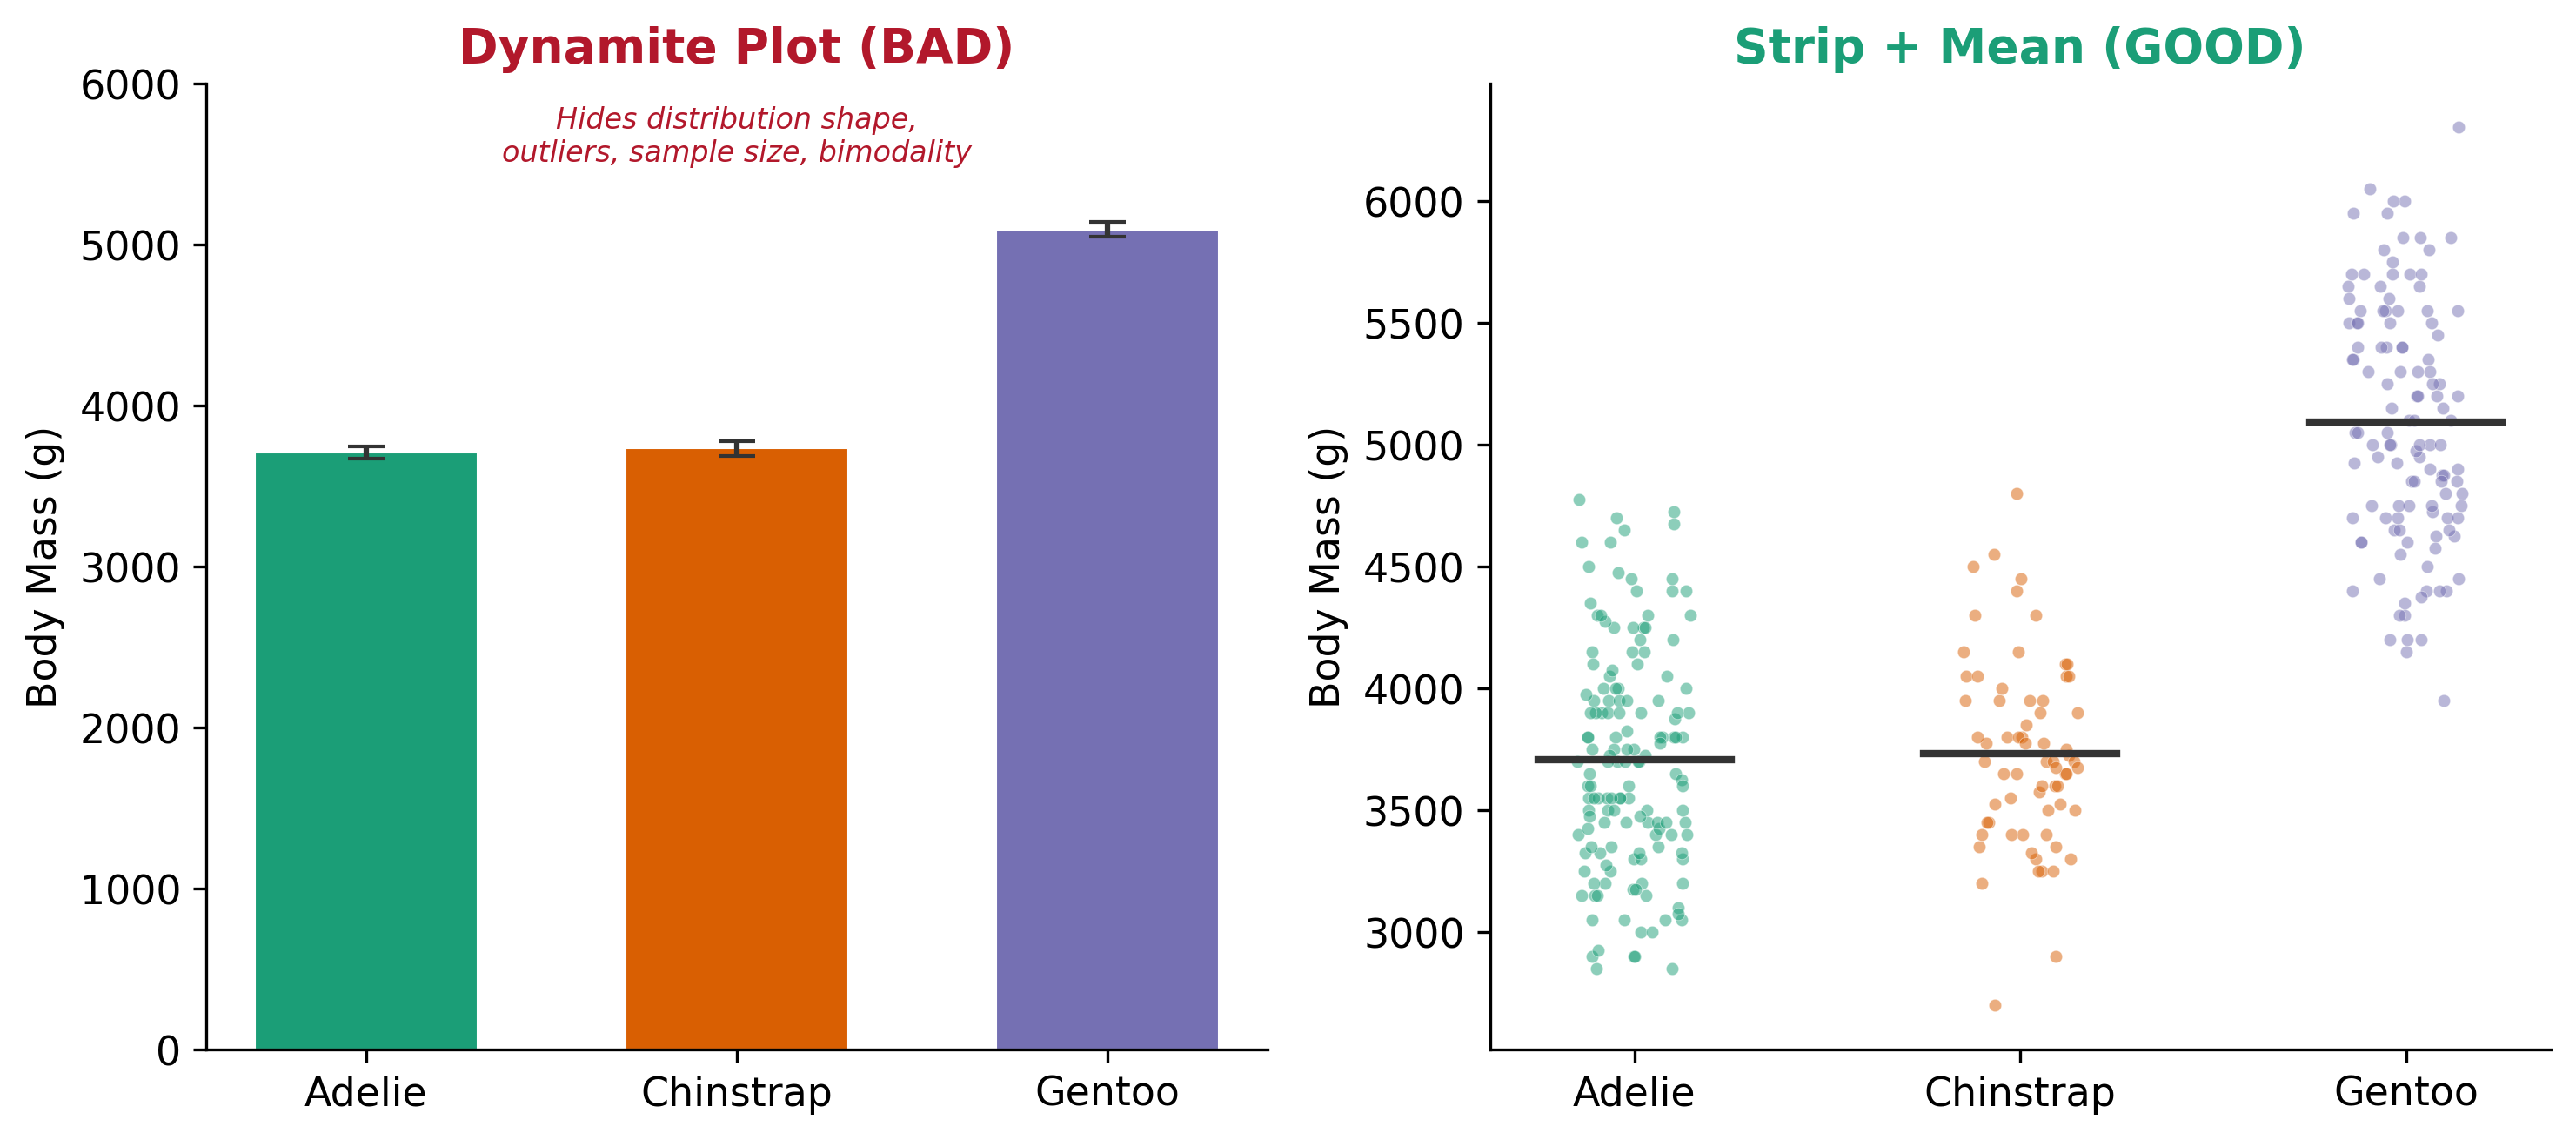
\includegraphics[width=0.88\textwidth]{m2_1_dynamite_vs_strip.png}

\vspace{0.2cm}
\begin{exampleblock}{Data Insight}
    \scriptsize Left: the ``dynamite plot'' (bar + error bar) shows only the mean and one interval. Distribution shape, outliers, sample size, and bimodality are \textbf{completely hidden}. Right: a strip plot reveals all individual observations plus the mean.
\end{exampleblock}
\end{frame}

% ── 4 ──
\begin{frame}{Why Dynamite Plots Are Harmful}
\smark{4/300}
\begin{columns}[T]
\begin{column}{0.50\textwidth}
\begin{itemize}
    \item The bar implies a \textbf{magnitude} starting at zero --- meaningless for most continuous measures
    \item The error bar is ambiguous: SE? SD? 95\% CI? Rarely labeled
    \item \textbf{n} is invisible --- a bar from $n=5$ looks identical to $n=500$
    \item Bimodality, skew, and outliers are erased
\end{itemize}
\end{column}
\begin{column}{0.47\textwidth}
\begin{alertblock}{Pro-Tip}
    \scriptsize Weissgerber et al.\ (2015, \textit{PLOS Biology}): ``Bar charts of continuous data should be replaced with more informative plots.'' Over 3{,}000 citations and counting.
\end{alertblock}
\vspace{0.2cm}
\begin{exampleblock}{Data Insight}
    \scriptsize Many journals now \textbf{reject} dynamite plots in submissions. Nature Methods, PLOS, eLife, and JBC all recommend showing raw data.
\end{exampleblock}
\end{column}
\end{columns}
\end{frame}

% ── 5 ──
\begin{frame}{Weissgerber's Demonstration}
\smark{5/300}
\centering
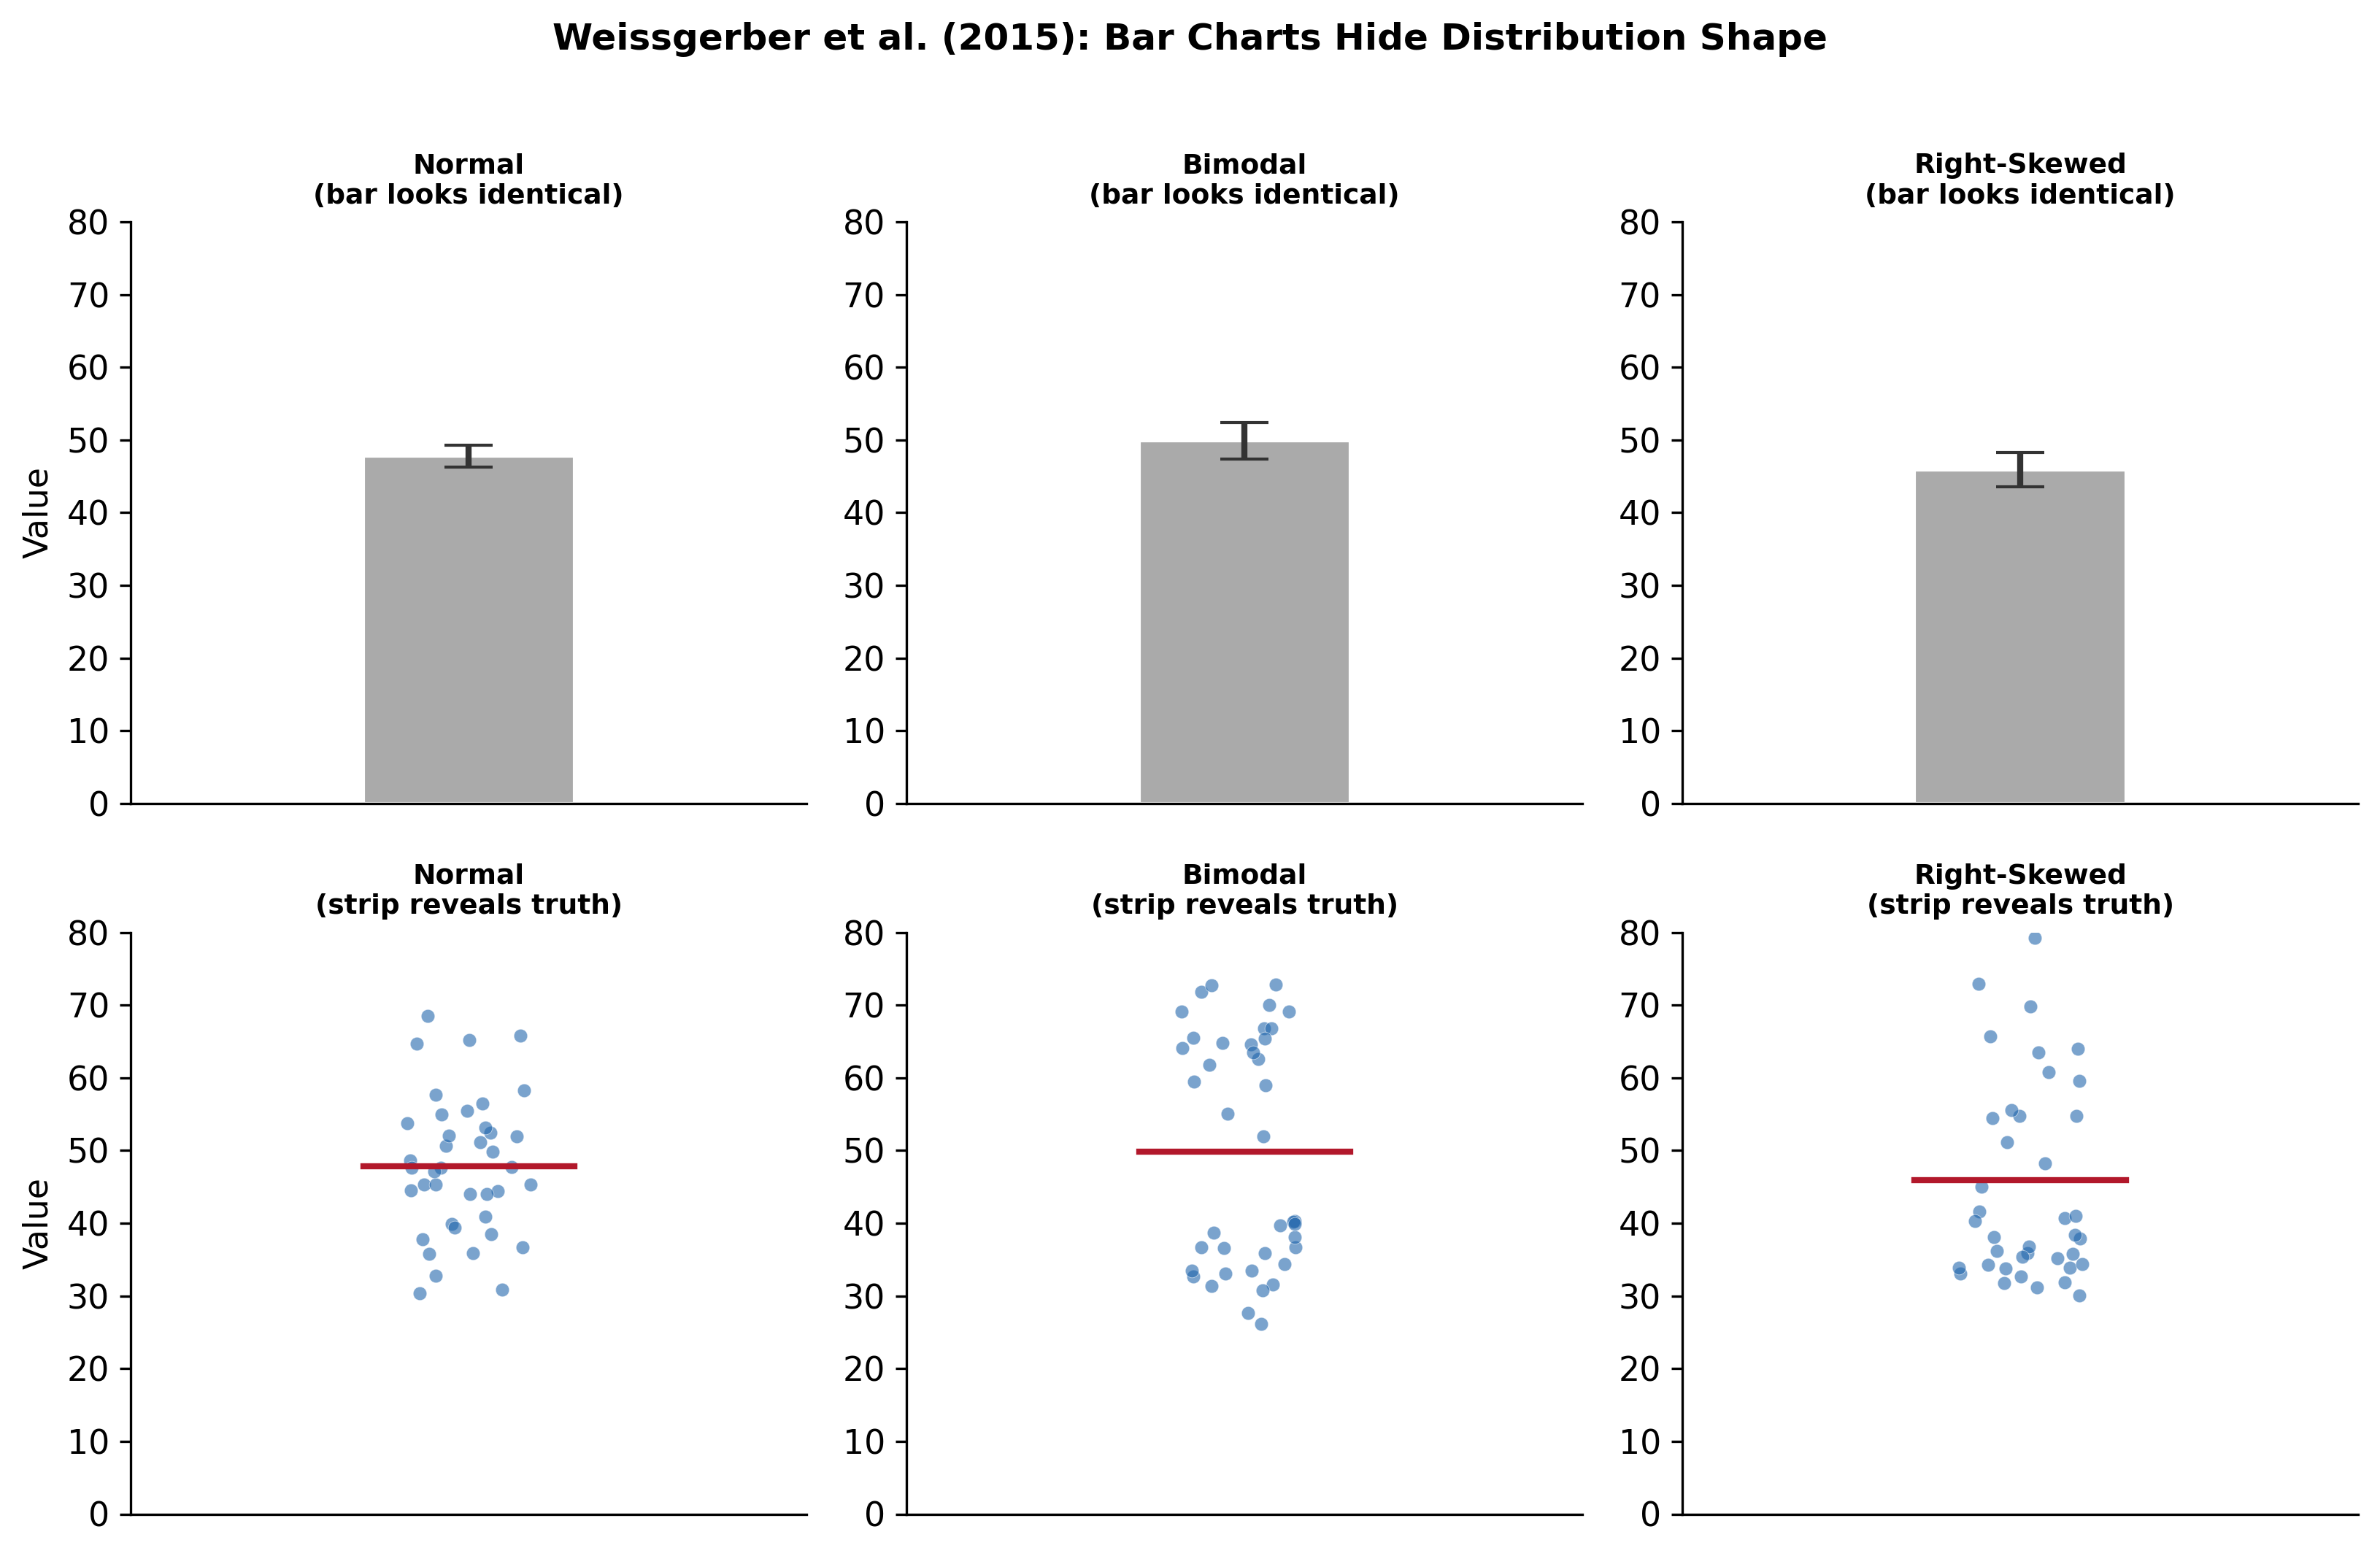
\includegraphics[width=0.88\textwidth]{m2_1_weissgerber.png}

\vspace{0.2cm}
\begin{exampleblock}{Data Insight}
    \scriptsize Top row: three bars with identical height and error. Bottom row: the raw data reveals a normal distribution, a bimodal distribution, and a right-skewed distribution. The bar chart could not distinguish them.
\end{exampleblock}
\end{frame}

% ── 6 ──
\begin{frame}{What Does Your Error Bar Mean?}
\smark{6/300}
\centering
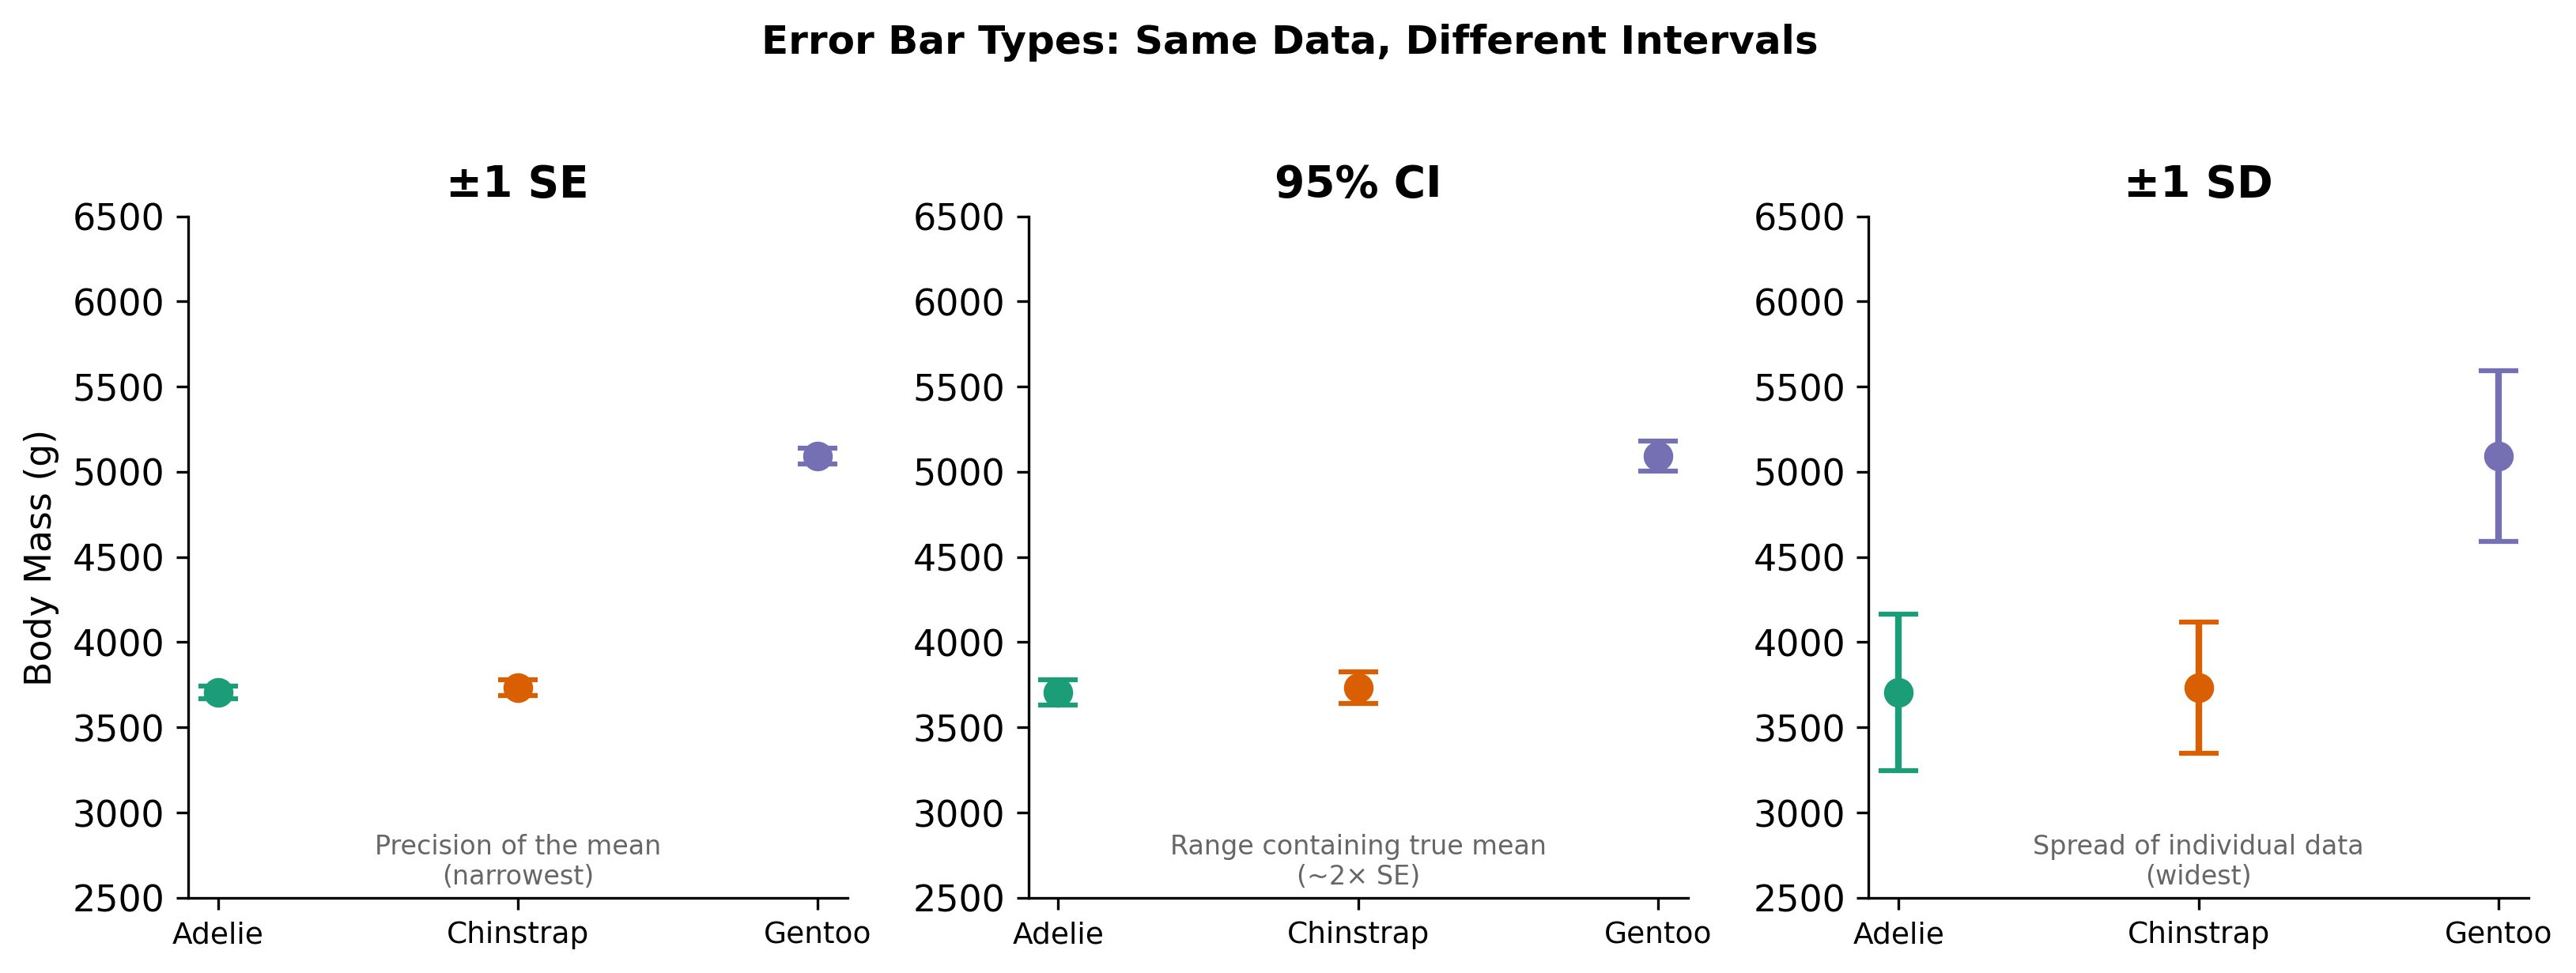
\includegraphics[width=0.88\textwidth]{m2_1_se_ci_sd.png}

\vspace{0.2cm}
\centering\small
\begin{tabular}{@{}lll@{}}
    \toprule
    \textbf{Interval} & \textbf{Formula} & \textbf{Interpretation} \\
    \midrule
    $\pm 1$ SE         & $s / \sqrt{n}$            & Precision of the mean estimate \\
    95\% CI            & $\bar{x} \pm 1.96 \cdot \text{SE}$ & Range likely containing true $\mu$ \\
    $\pm 1$ SD         & $s$                        & Spread of individual observations \\
    \bottomrule
\end{tabular}
\end{frame}

% ── 7 ──
\begin{frame}{SE vs.\ CI vs.\ SD: When to Use Which}
\smark{7/300}
\begin{columns}[T]
\begin{column}{0.50\textwidth}
\begin{itemize}
    \item \textbf{SE}: comparing means across groups (is the difference significant?)
    \item \textbf{95\% CI}: inferential statement (where does $\mu$ plausibly lie?)
    \item \textbf{SD}: describing variability of individual data (how spread out are subjects?)
\end{itemize}
\end{column}
\begin{column}{0.47\textwidth}
\begin{alertblock}{Pro-Tip}
    \scriptsize \textbf{Always label your error bars.} ``Error bars represent $\pm$1 SE'' in the caption. An unlabeled error bar is meaningless --- the reader cannot interpret it.
\end{alertblock}
\vspace{0.2cm}
\begin{exampleblock}{Data Insight}
    \scriptsize Non-overlapping 95\% CIs $\Rightarrow$ $p < 0.05$ (approximately). Overlapping CIs do \textbf{not} imply $p > 0.05$ --- the rule is asymmetric. Use formal tests for inference.
\end{exampleblock}
\end{column}
\end{columns}
\end{frame}

% ── 8 ──
\begin{frame}[fragile]{Error Bars --- \Rlang}\smark{8/300}
\begin{columns}[T]
\begin{column}{0.55\textwidth}
\begin{lstlisting}[style=Rstyle]
# Mean + SE (built-in)
ggplot(penguins,
  aes(species, body_mass_g)) +
  stat_summary(fun.data=mean_se,
    geom="pointrange",
    size=0.8) +
  theme_minimal()

# Mean + 95% CI via Hmisc
library(Hmisc)
ggplot(penguins,
  aes(species, body_mass_g)) +
  stat_summary(
    fun.data=mean_cl_boot,
    geom="pointrange") +
  theme_minimal()
\end{lstlisting}
\end{column}
\begin{column}{0.42\textwidth}
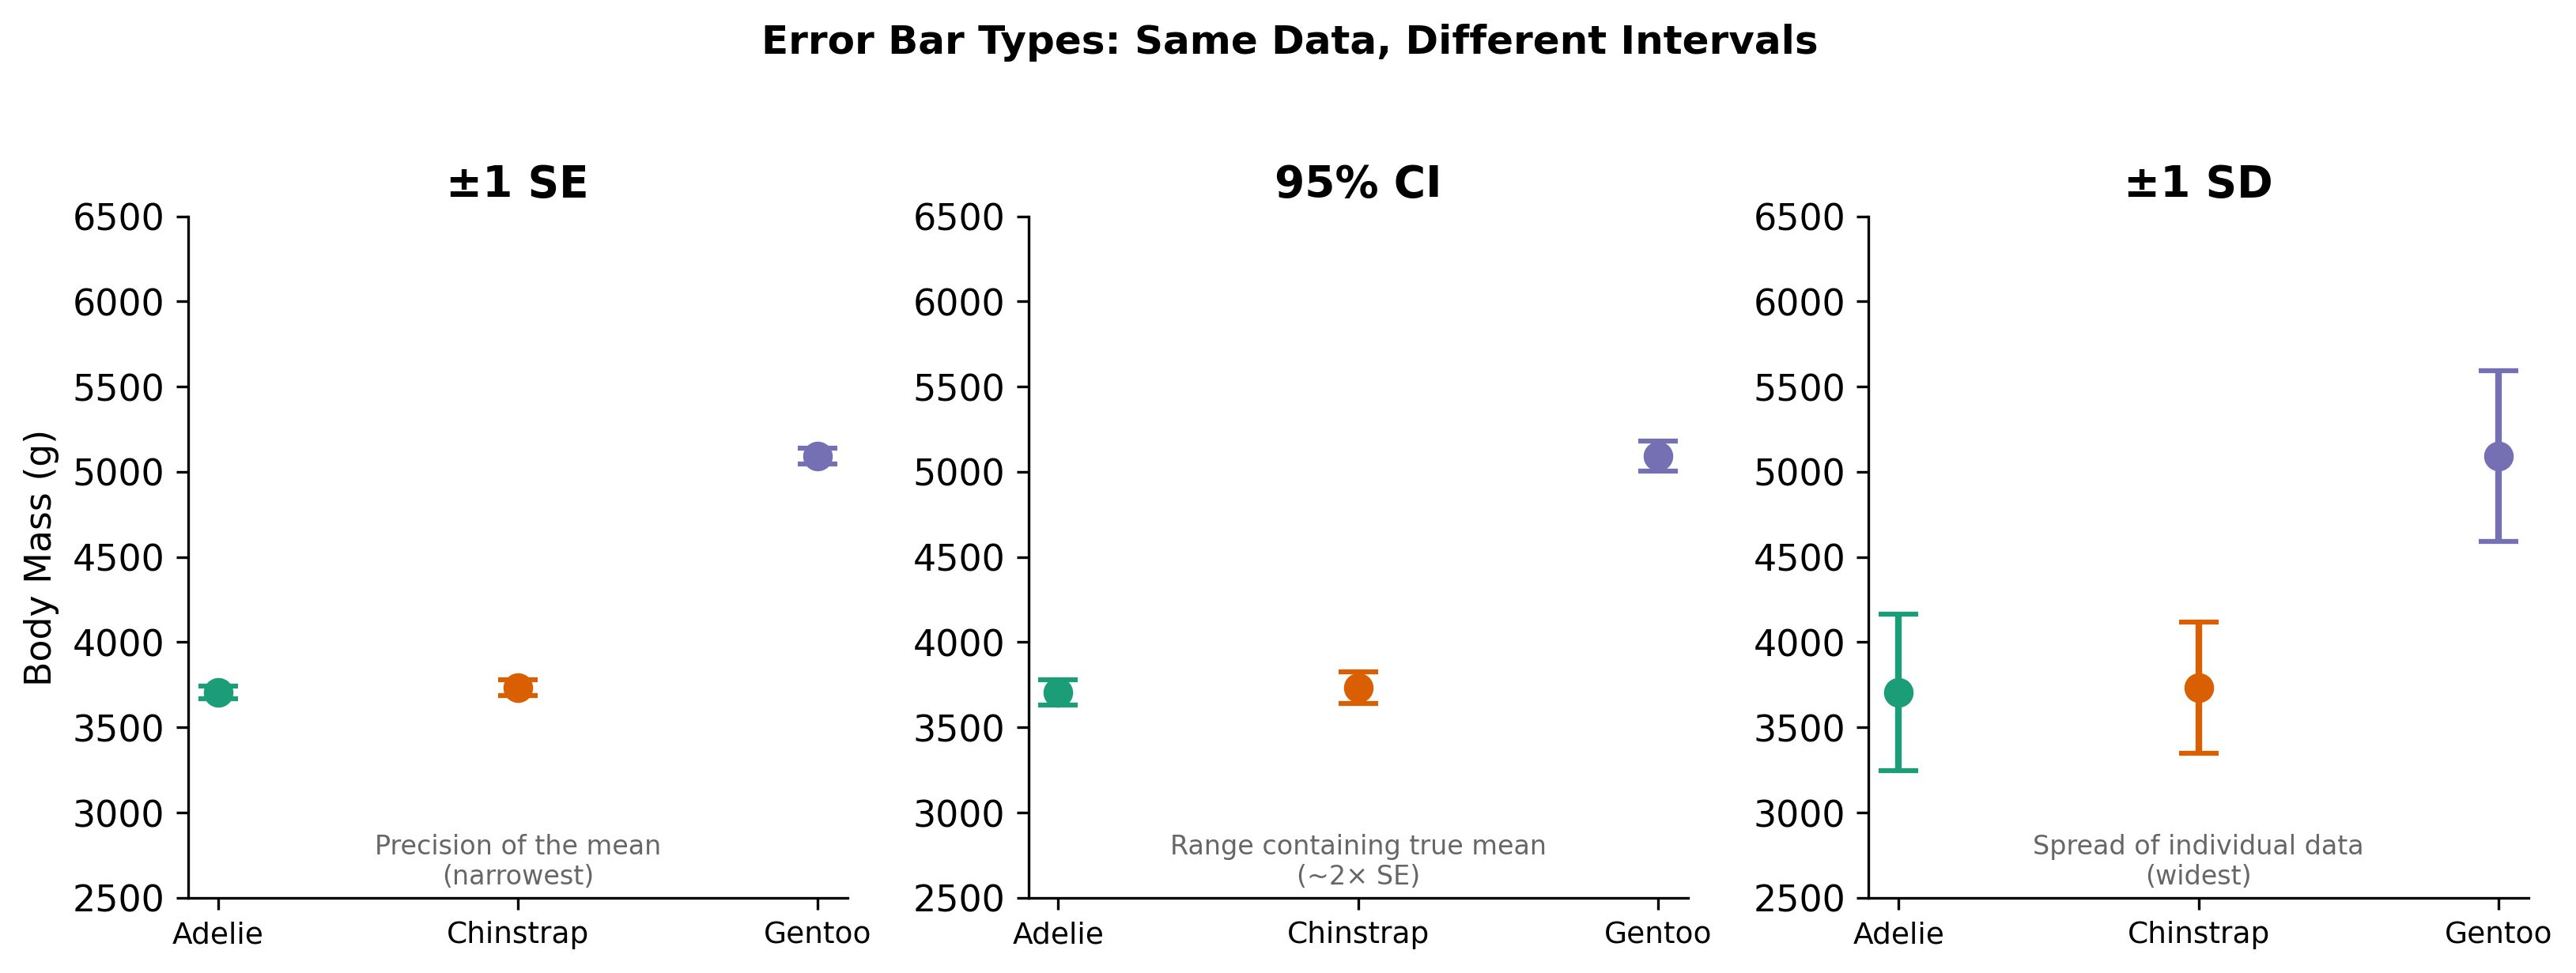
\includegraphics[width=\textwidth]{m2_1_se_ci_sd.png}
\begin{alertblock}{Pro-Tip}
    \scriptsize \texttt{mean\_se} = $\bar{x} \pm \text{SE}$. \texttt{mean\_cl\_boot} = bootstrap 95\% CI. \texttt{mean\_cl\_normal} = normal-theory CI. All work inside \texttt{stat\_summary()}.
\end{alertblock}
\end{column}
\end{columns}
\end{frame}

% ── 9 ──
\begin{frame}[fragile]{Error Bars --- \Python}\smark{9/300}
\begin{columns}[T]
\begin{column}{0.55\textwidth}
\begin{lstlisting}[style=Pystyle]
# seaborn pointplot (mean + CI)
sns.pointplot(data=penguins,
    x="species", y="body_mass_g",
    errorbar="se",  # or "ci", "sd"
    capsize=0.15,
    color="#B2182B")

# Manual with scipy bootstrap
from scipy.stats import bootstrap
data = (penguins.query(
    "species=='Adelie'")
    ["body_mass_g"].values,)
res = bootstrap(data,
    np.mean, n_resamples=5000,
    confidence_level=0.95)
ci_lo = res.confidence_interval.low
ci_hi = res.confidence_interval.high
\end{lstlisting}
\end{column}
\begin{column}{0.42\textwidth}
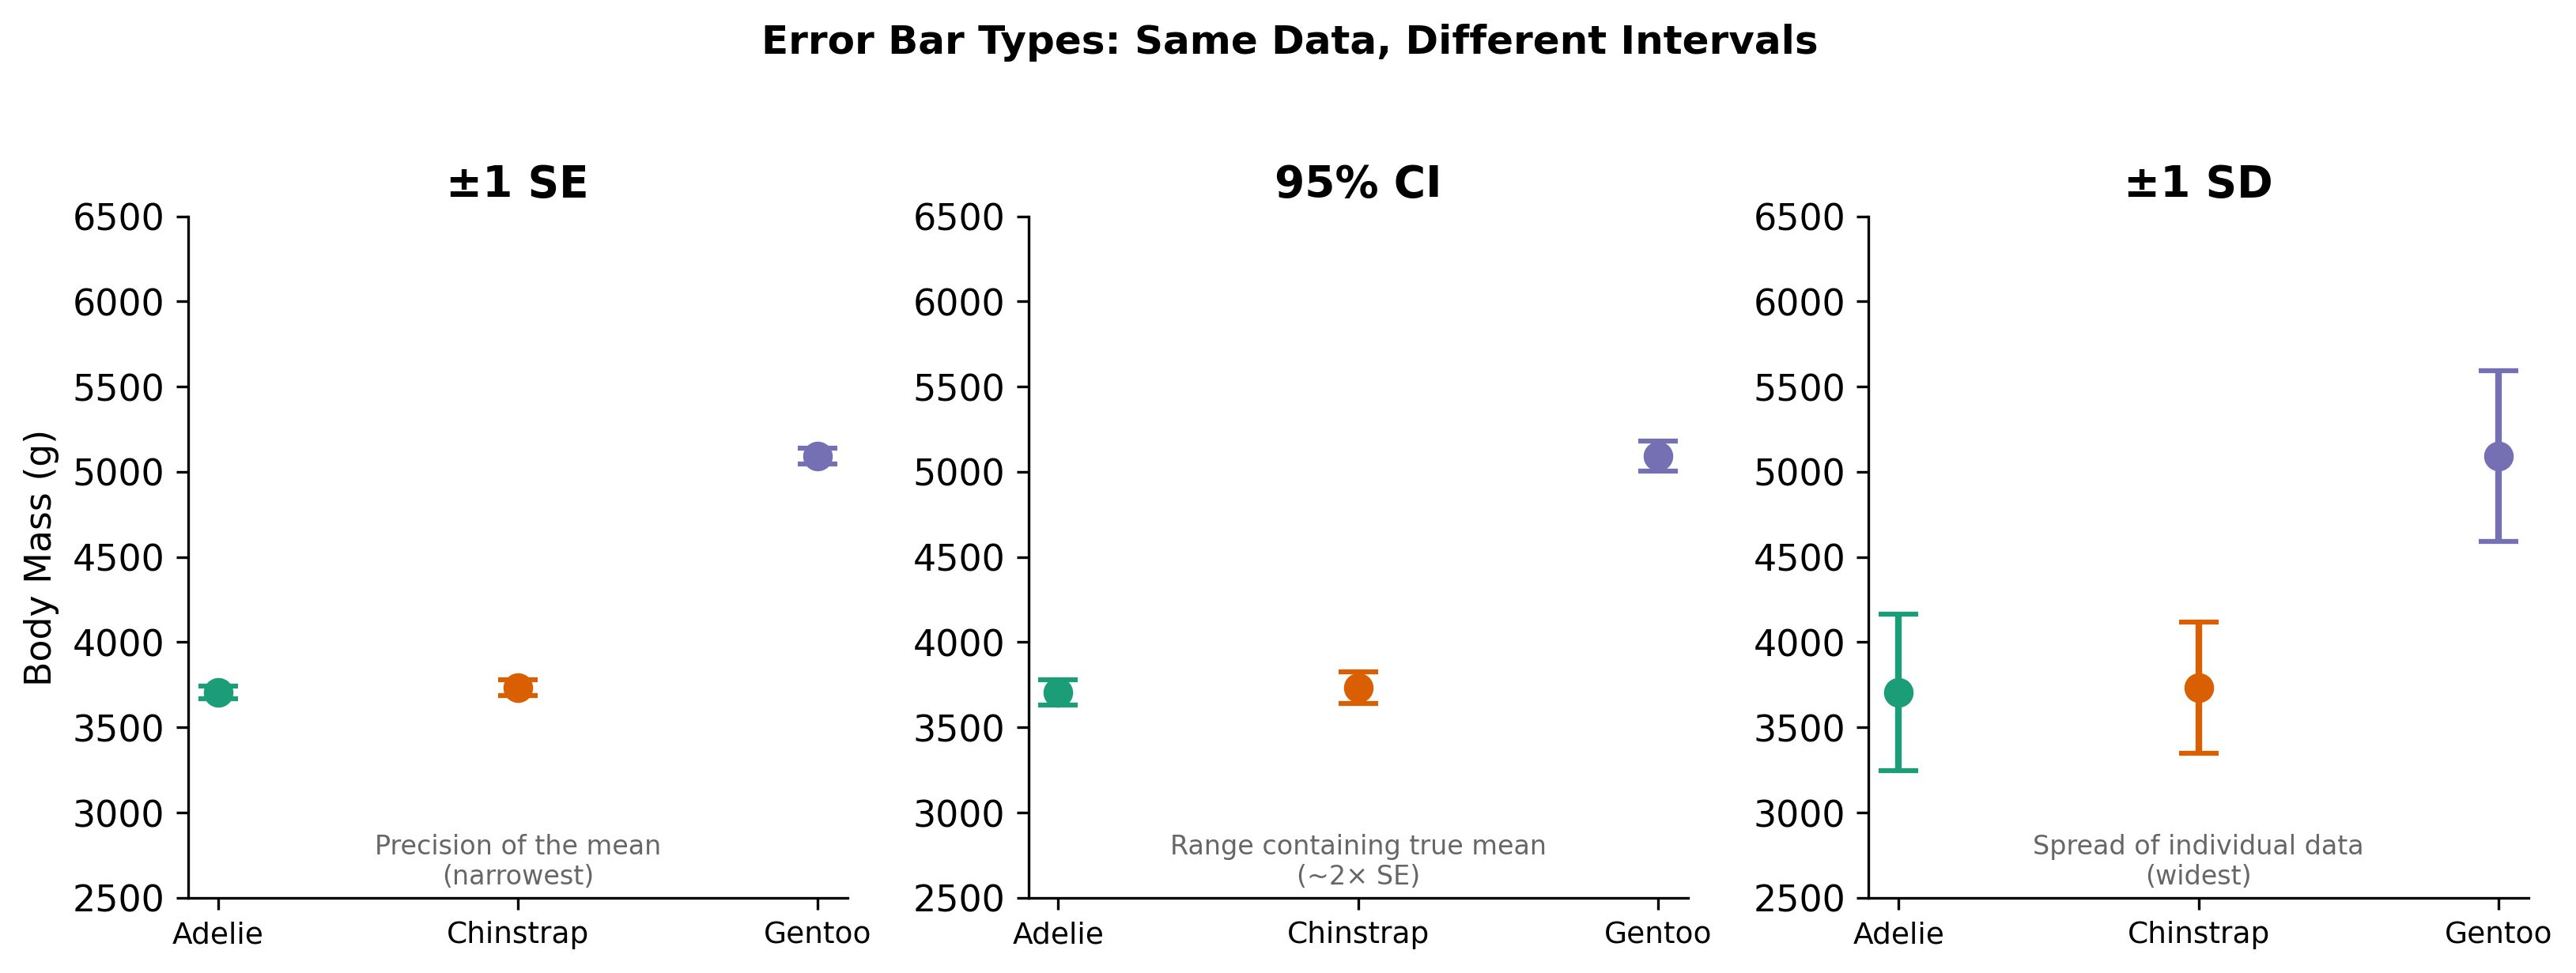
\includegraphics[width=\textwidth]{m2_1_se_ci_sd.png}
\begin{exampleblock}{Data Insight}
    \scriptsize seaborn 0.12+ uses \texttt{errorbar=} parameter: \texttt{"se"}, \texttt{"sd"}, \texttt{("ci", 95)}, or \texttt{("pi", 95)} for prediction intervals.
\end{exampleblock}
\end{column}
\end{columns}
\end{frame}

% ── 10 ──
\begin{frame}{The Strip Plot: Show Every Observation}
\smark{10/300}
\begin{columns}[T]
\begin{column}{0.50\textwidth}
\begin{itemize}
    \item Plot \textbf{every data point} as a jittered dot
    \item Reader sees sample size, distribution shape, outliers immediately
    \item Overlay mean $\pm$ CI on top for inference
    \item Works for $n \leq 200$; beyond that, use violin or density
\end{itemize}
\end{column}
\begin{column}{0.47\textwidth}
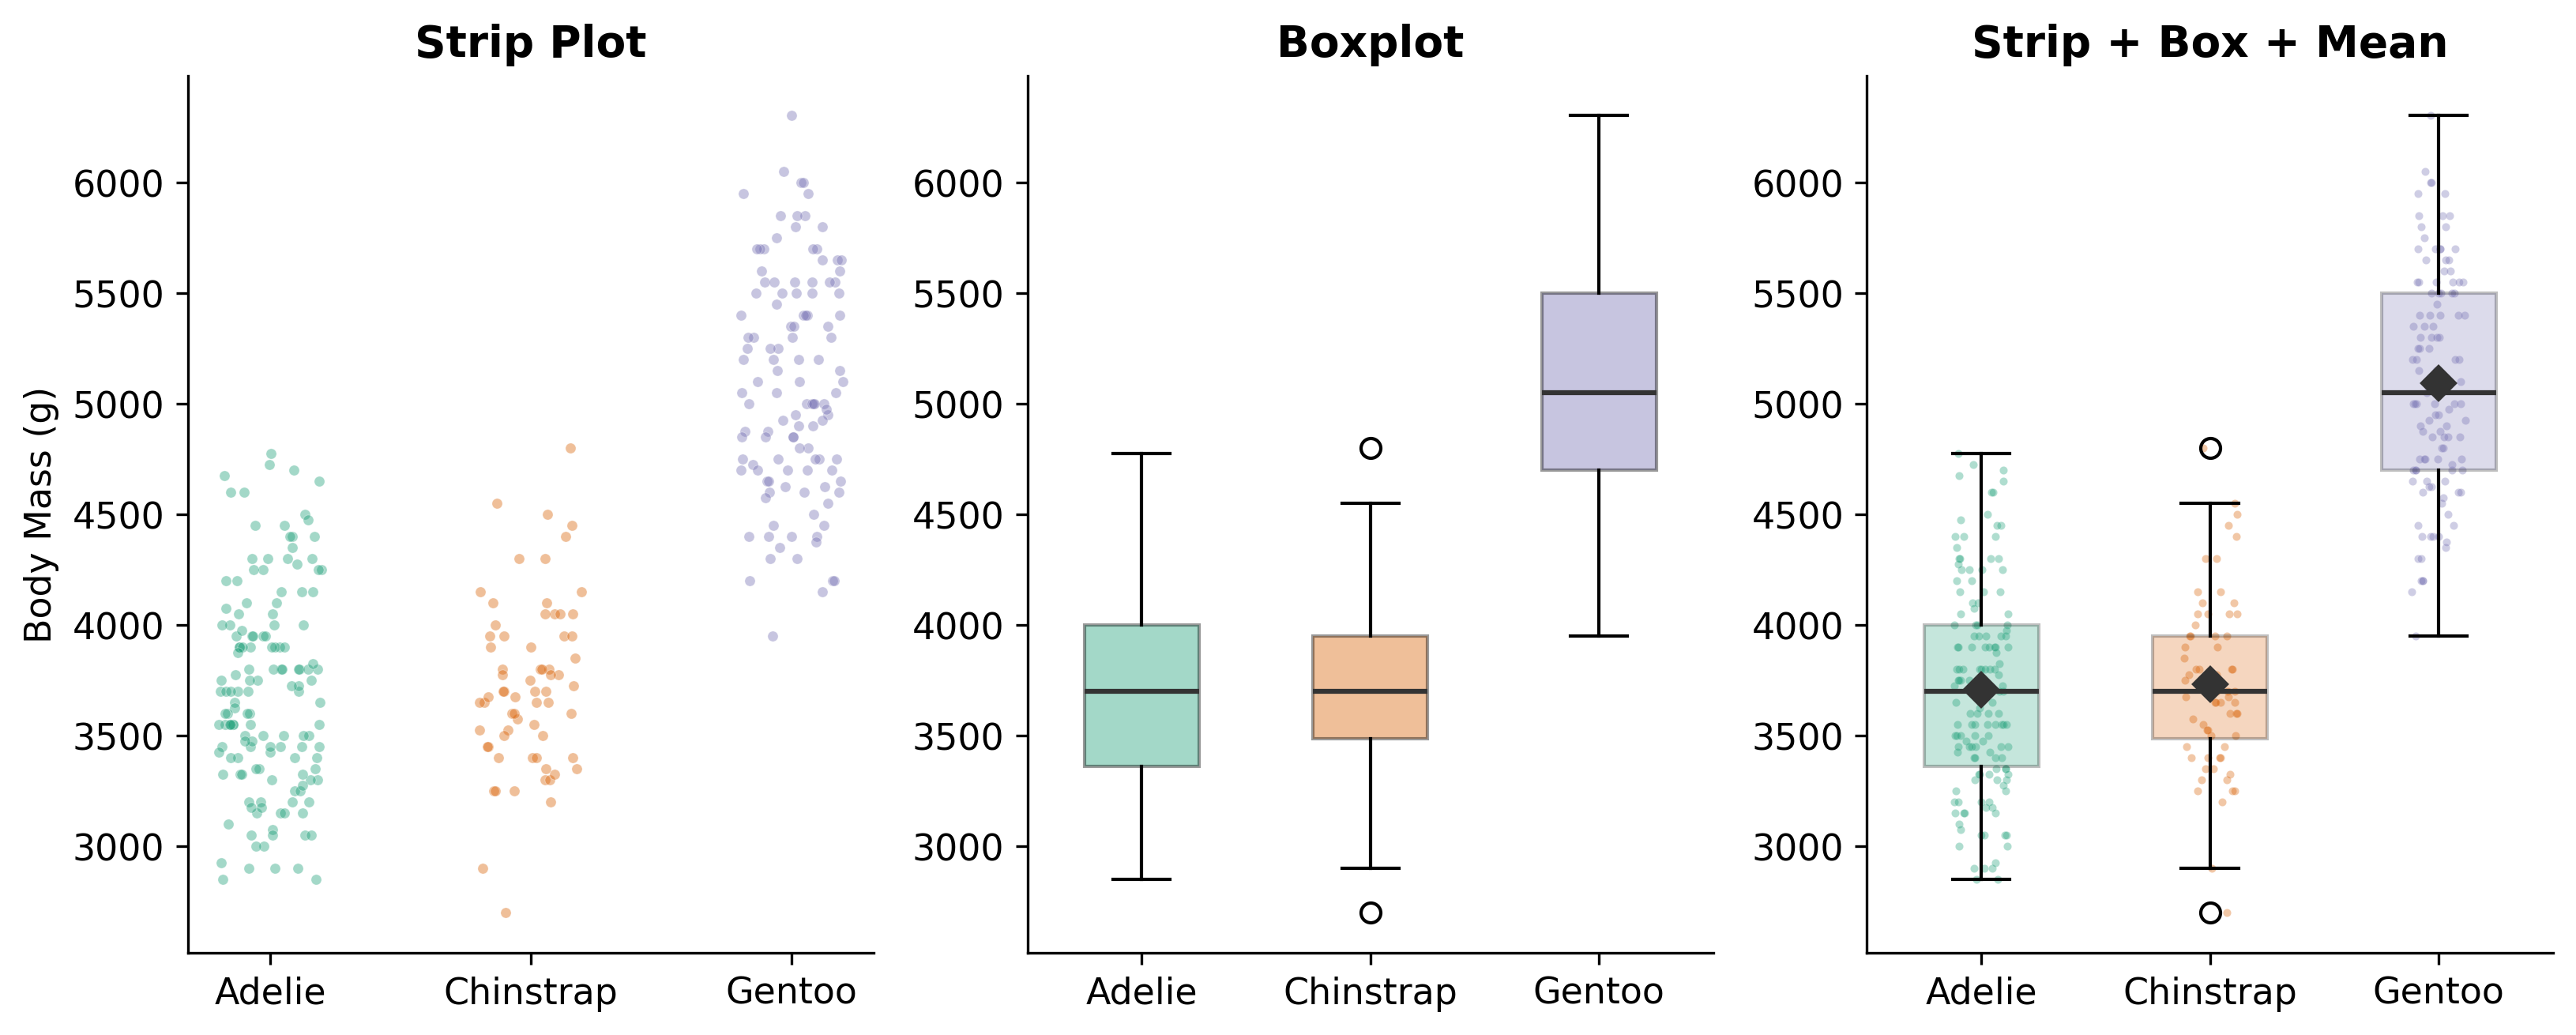
\includegraphics[width=\textwidth]{m2_1_strip_box_mean.png}
\begin{exampleblock}{Data Insight}
    \scriptsize Left: raw strip. Center: boxplot (summary). Right: hybrid (strip + box + mean diamond). The hybrid gives the most information per pixel.
\end{exampleblock}
\end{column}
\end{columns}
\end{frame}

% ── 11 ──
\begin{frame}[fragile]{Strip Plot --- \Rlang}\smark{11/300}
\begin{columns}[T]
\begin{column}{0.55\textwidth}
\begin{lstlisting}[style=Rstyle]
# Basic strip
ggplot(penguins,
  aes(species, body_mass_g,
      color = species)) +
  geom_jitter(width=0.2,
    alpha=0.5, size=1.5) +
  stat_summary(fun=mean,
    geom="point", shape=18,
    size=4, color="black") +
  theme_minimal() +
  theme(legend.position="none")
\end{lstlisting}
\end{column}
\begin{column}{0.42\textwidth}
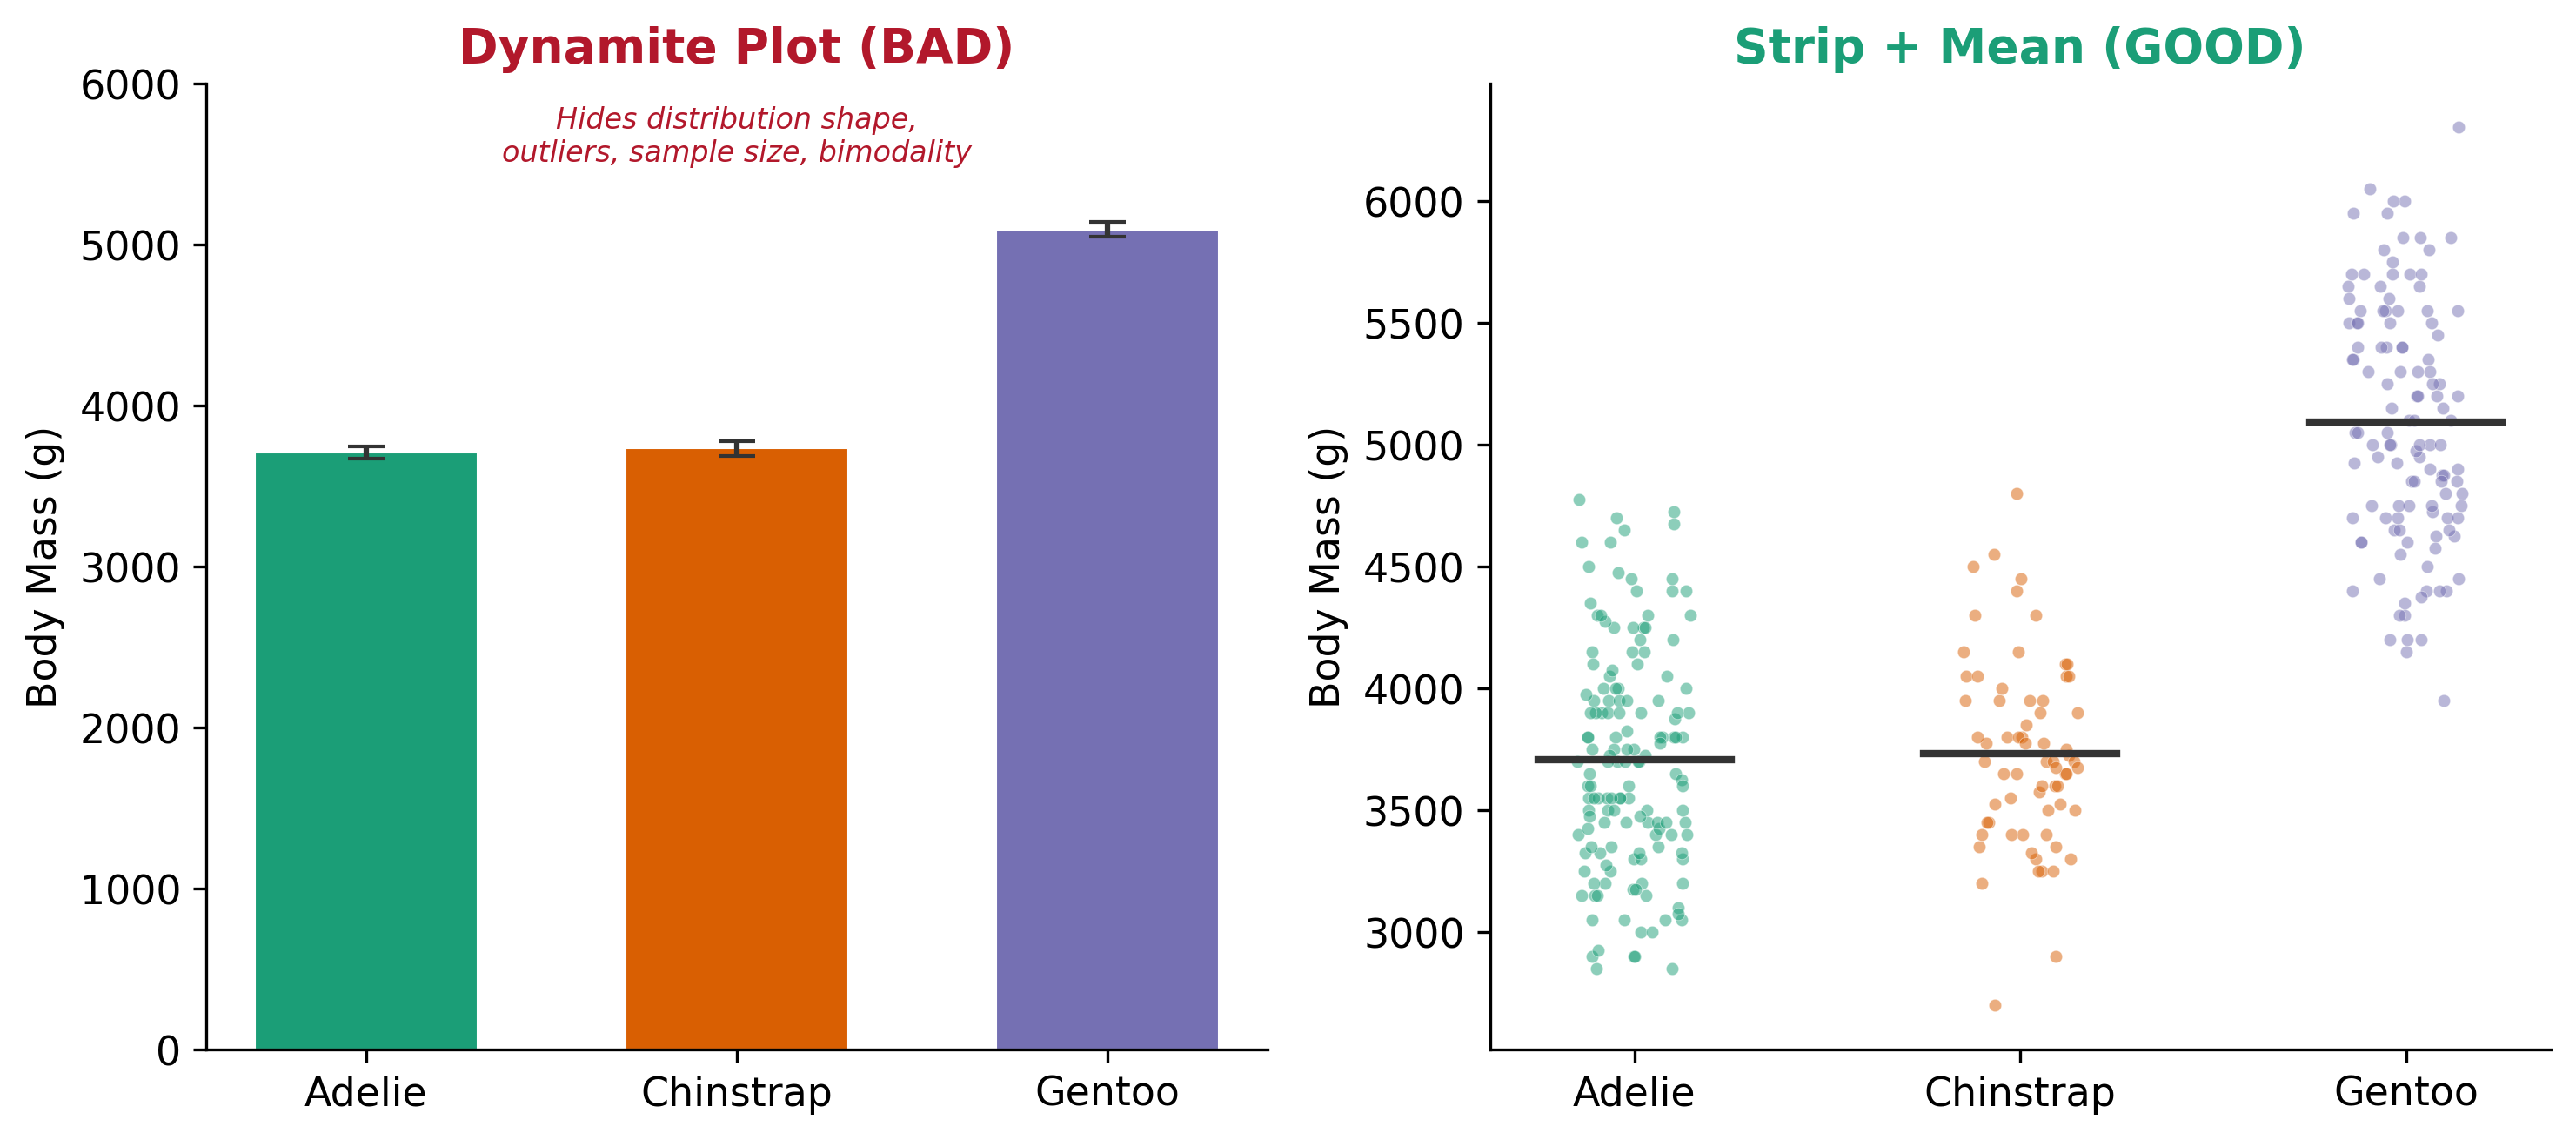
\includegraphics[width=\textwidth]{m2_1_dynamite_vs_strip.png}
\begin{alertblock}{Pro-Tip}
    \scriptsize \texttt{shape=18} is a diamond --- a good marker for the mean because it is visually distinct from the jittered circles.
\end{alertblock}
\end{column}
\end{columns}
\end{frame}

% ── 12 ──
\begin{frame}[fragile]{Strip Plot --- \Python}\smark{12/300}
\begin{columns}[T]
\begin{column}{0.55\textwidth}
\begin{lstlisting}[style=Pystyle]
# seaborn stripplot + mean
fig, ax = plt.subplots()
sns.stripplot(data=penguins,
    x="species", y="body_mass_g",
    jitter=0.2, alpha=0.5, s=3,
    hue="species", legend=False,
    ax=ax)

# Overlay means
means = penguins.groupby("species")\
    ["body_mass_g"].mean()
ax.scatter(range(3), means,
    marker="D", s=80, color="black",
    zorder=5, label="Mean")
ax.legend()
\end{lstlisting}
\end{column}
\begin{column}{0.42\textwidth}
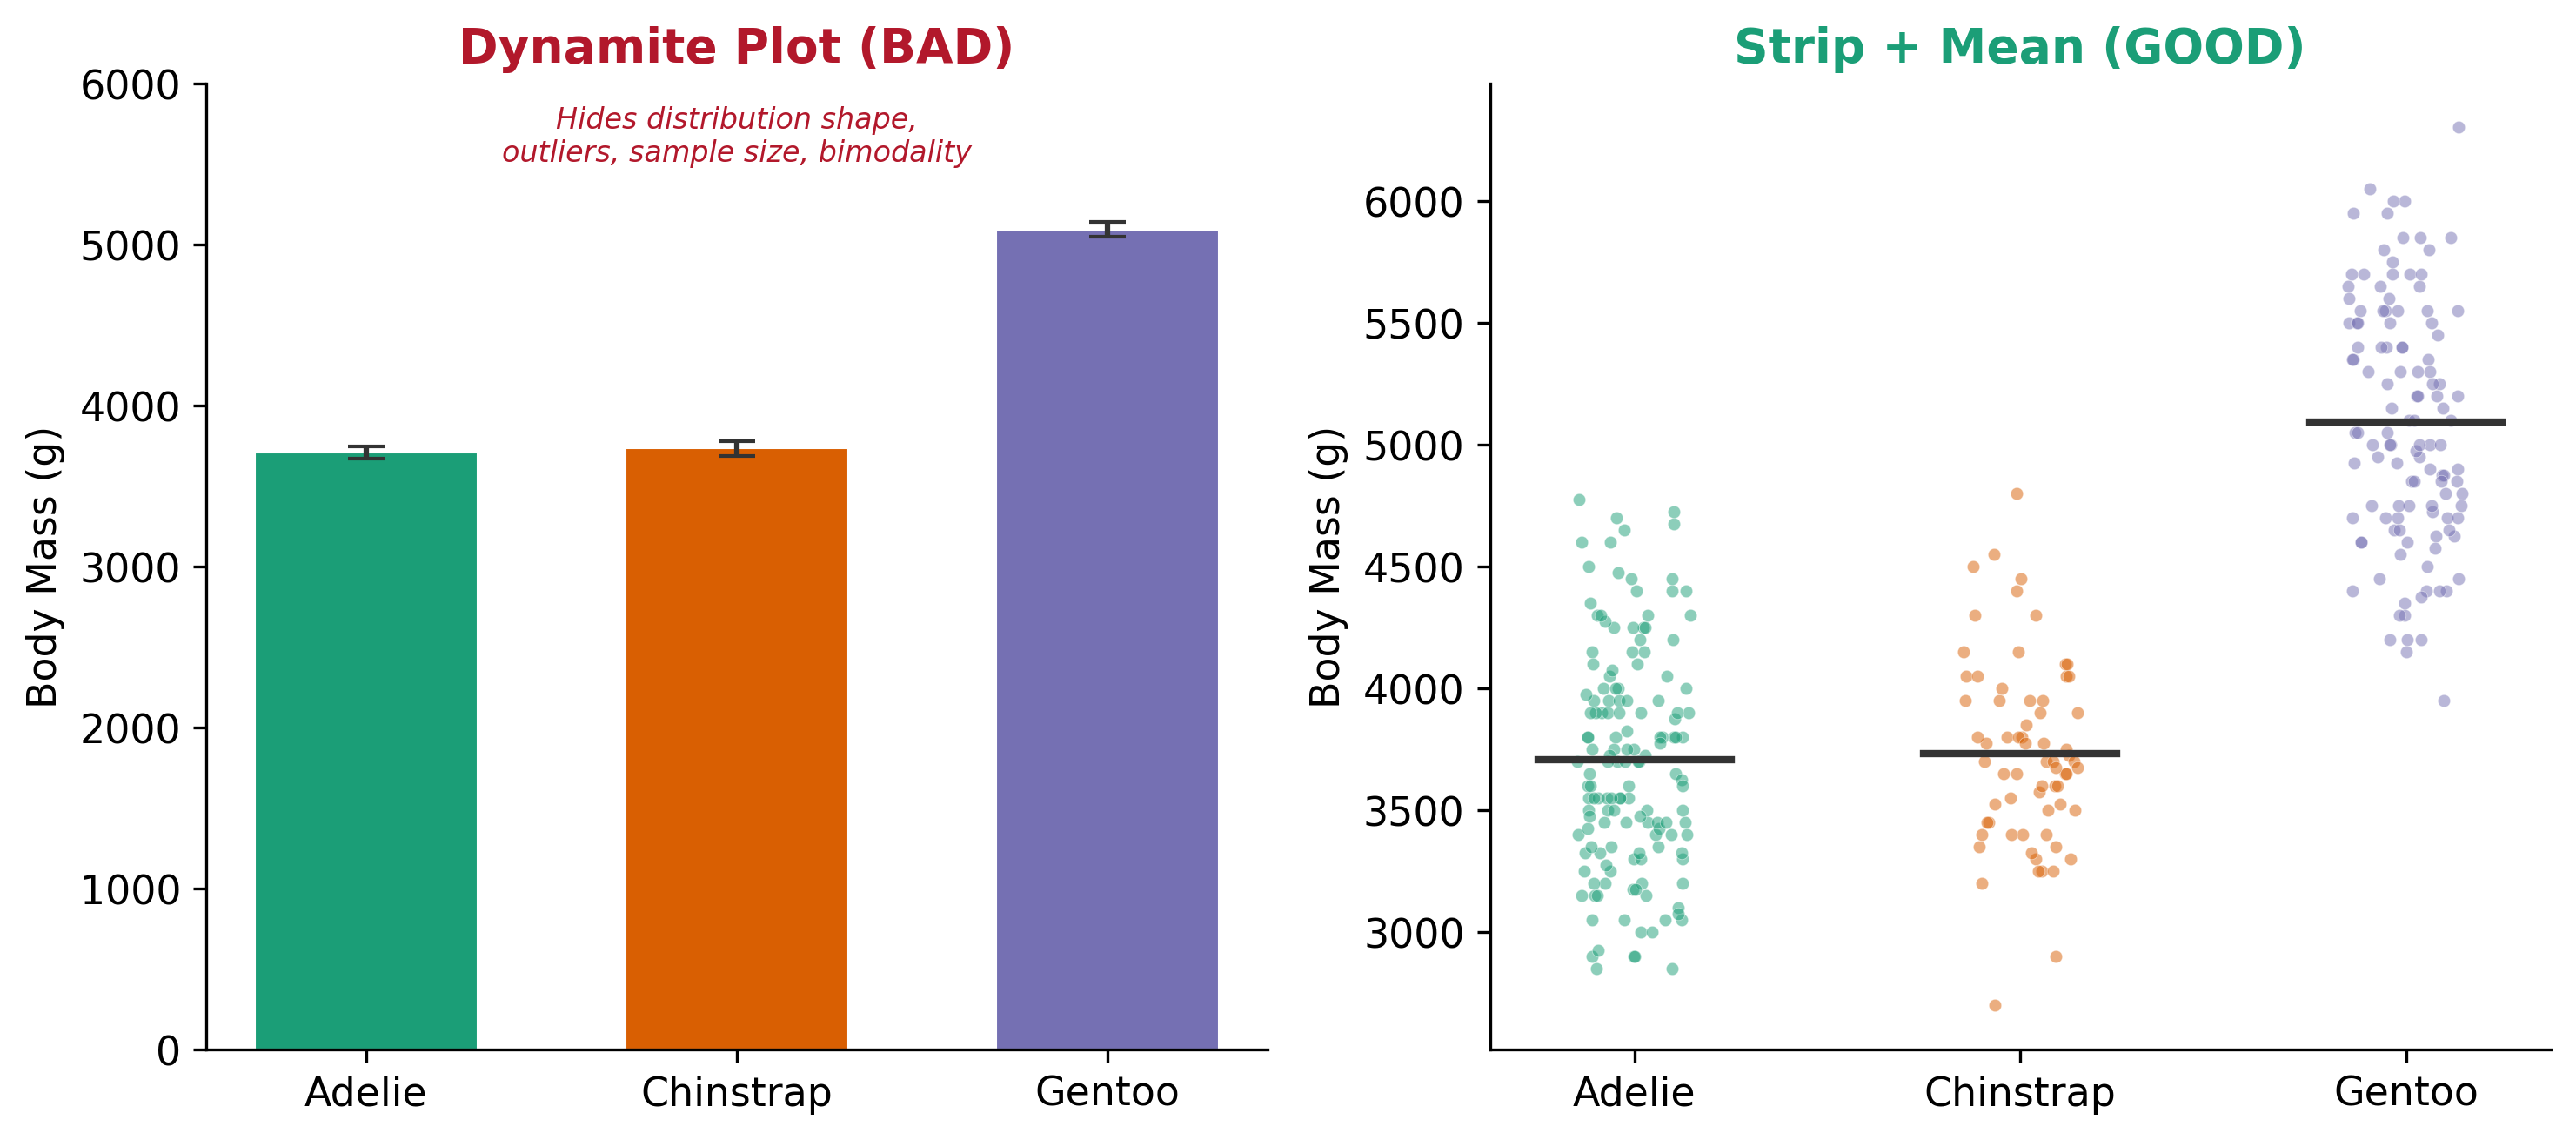
\includegraphics[width=\textwidth]{m2_1_dynamite_vs_strip.png}
\begin{exampleblock}{Data Insight}
    \scriptsize seaborn's \texttt{stripplot()} handles the jittering. Overlay the mean manually with \texttt{ax.scatter()}.
\end{exampleblock}
\end{column}
\end{columns}
\end{frame}

% ── 13 ──
\begin{frame}{Summary Geoms: pointrange, crossbar, errorbar}
\smark{13/300}
\centering
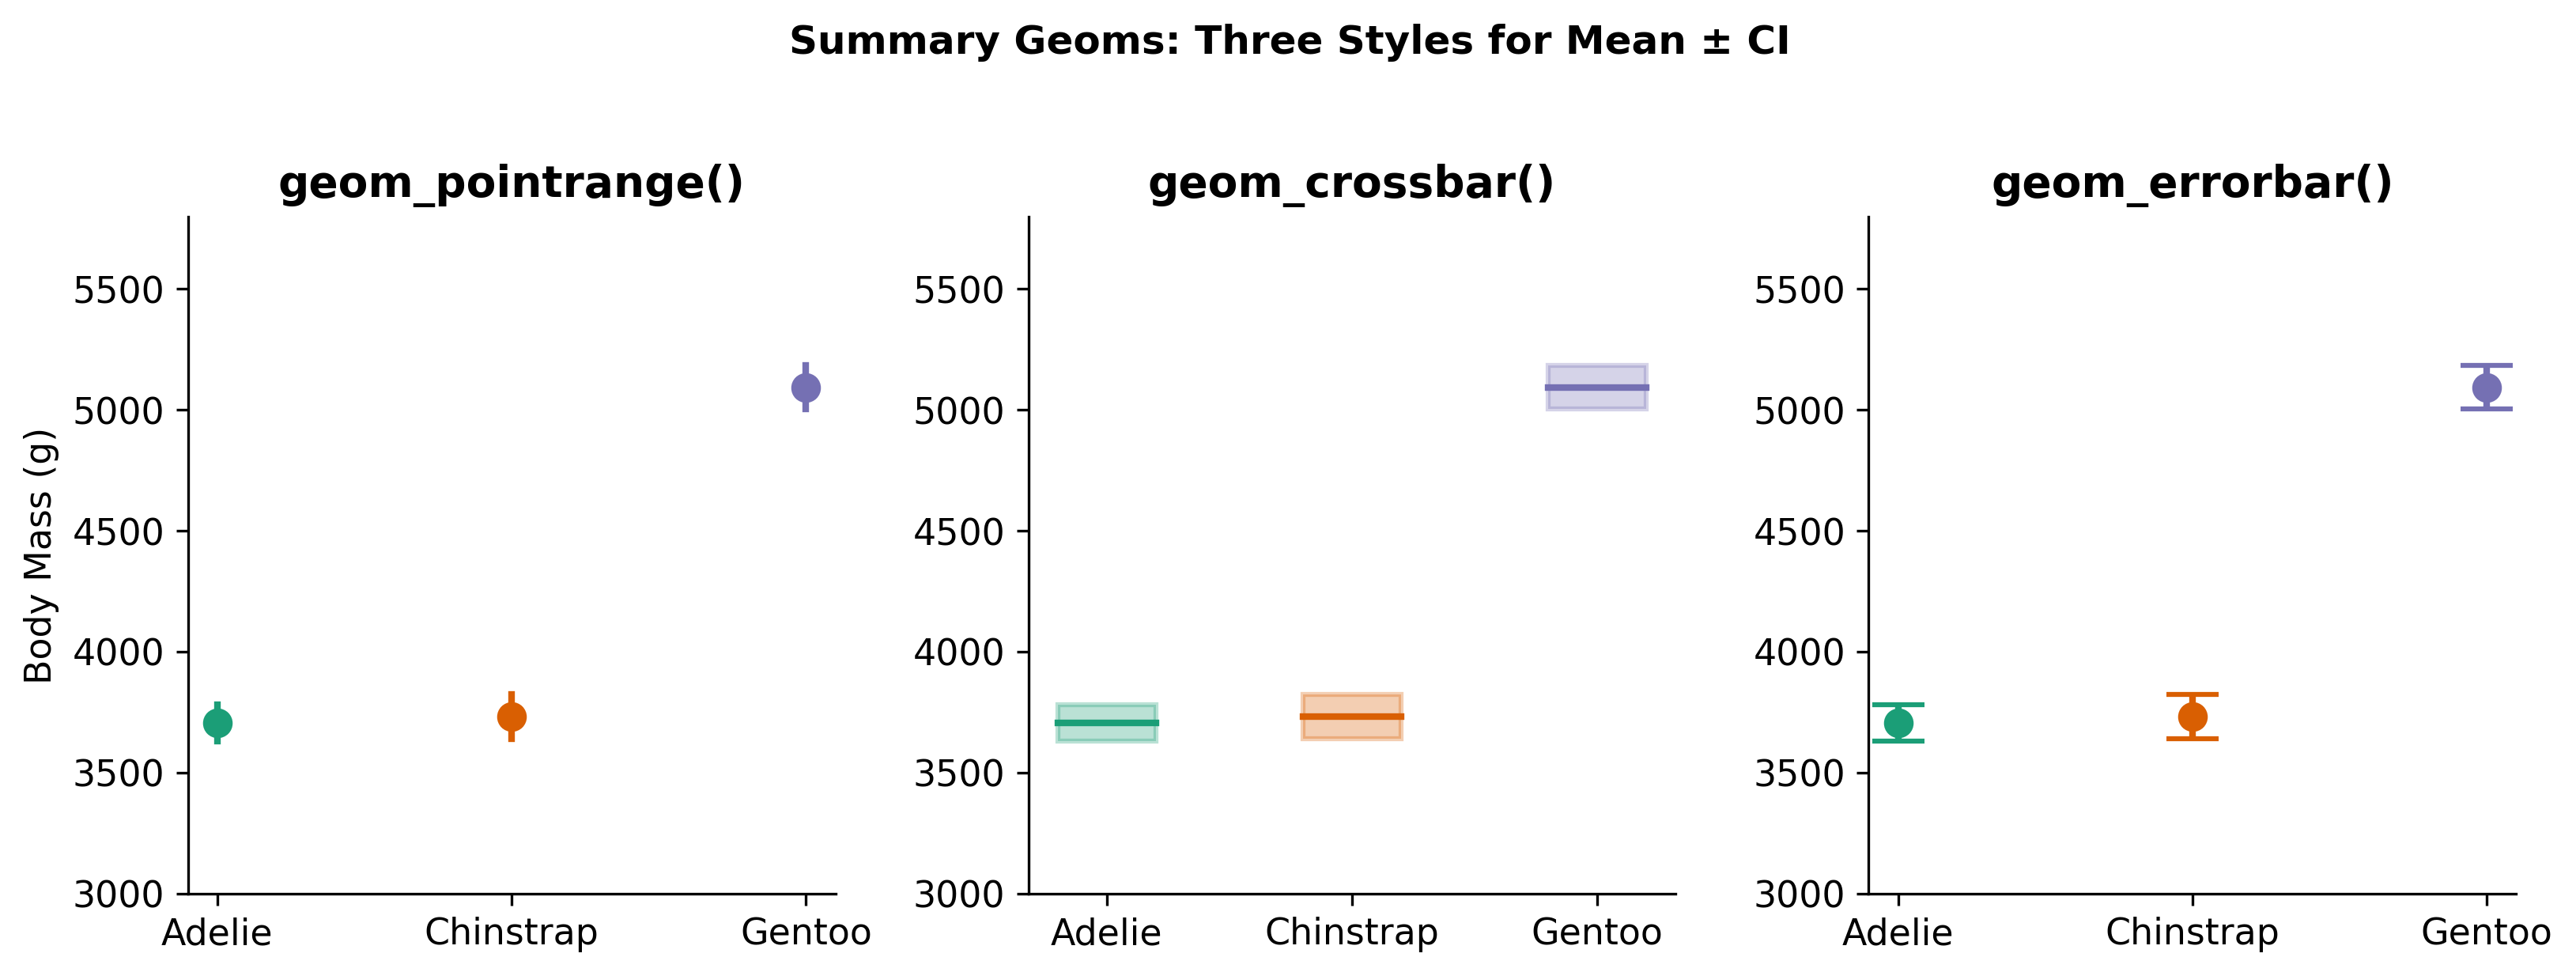
\includegraphics[width=0.88\textwidth]{m2_1_summary_geoms.png}

\vspace{0.2cm}
\centering\small
\begin{tabular}{@{}lll@{}}
    \toprule
    \textbf{Geom} & \textbf{Visual} & \textbf{Best For} \\
    \midrule
    \texttt{geom\_pointrange} & Point + vertical line   & Default choice \\
    \texttt{geom\_crossbar}   & Horizontal bar + box    & Emphasize the interval width \\
    \texttt{geom\_errorbar}   & Capped whiskers         & Traditional (but more ink) \\
    \bottomrule
\end{tabular}
\end{frame}

% ── 14 ──
\begin{frame}[fragile]{Summary Geoms --- \Rlang}\smark{14/300}
\begin{columns}[T]
\begin{column}{0.55\textwidth}
\begin{lstlisting}[style=Rstyle]
# pointrange (recommended)
ggplot(penguins,
  aes(species, body_mass_g)) +
  stat_summary(
    fun.data = mean_se,
    geom = "pointrange",
    color = "#2166AC",
    size = 0.8)

# crossbar
stat_summary(fun.data=mean_se,
  geom = "crossbar", width=0.3)

# errorbar
stat_summary(fun.data=mean_se,
  geom = "errorbar", width=0.2)
\end{lstlisting}
\end{column}
\begin{column}{0.42\textwidth}
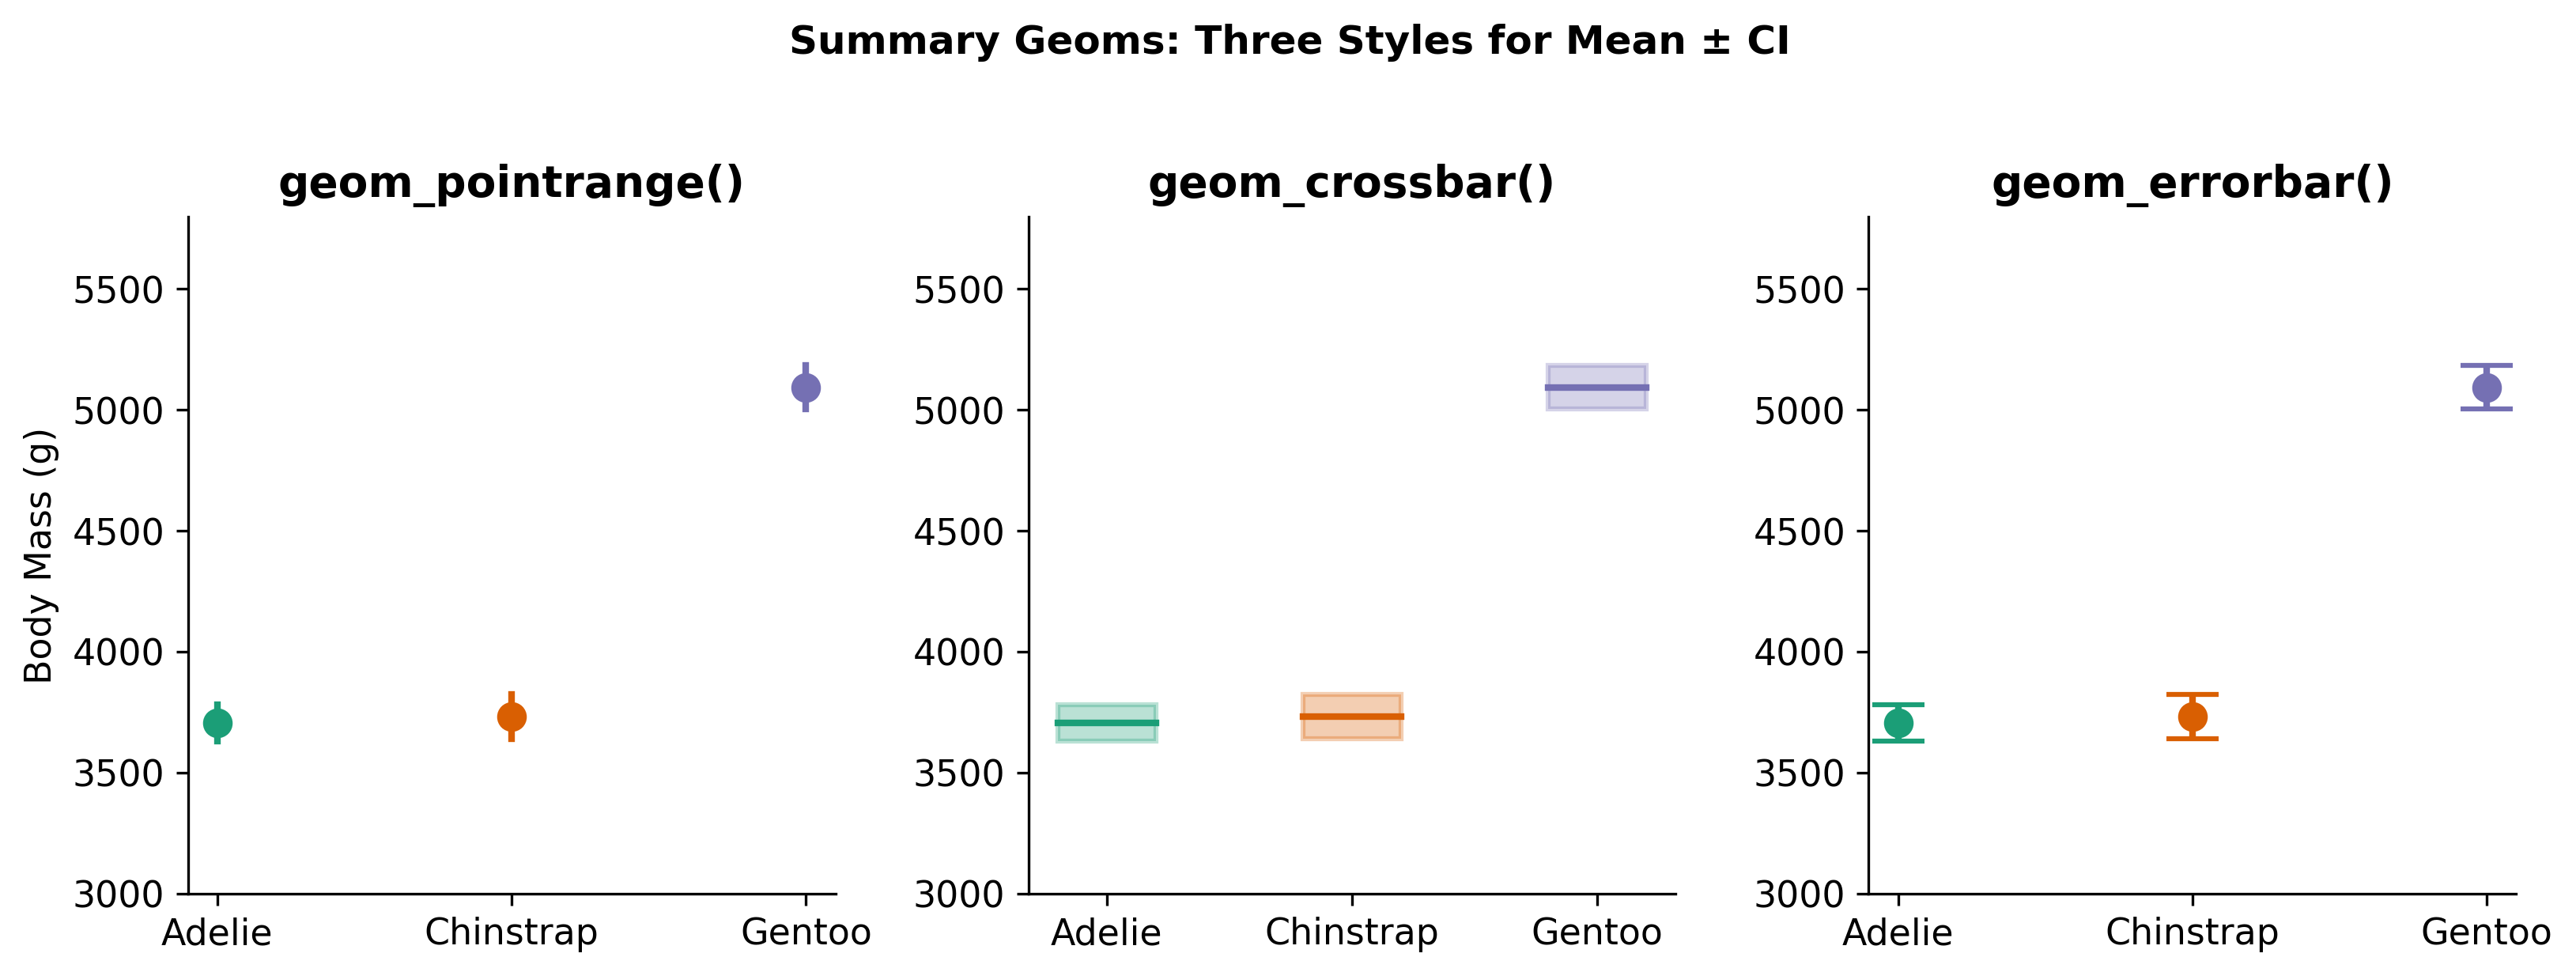
\includegraphics[width=\textwidth]{m2_1_summary_geoms.png}
\begin{alertblock}{Pro-Tip}
    \scriptsize \texttt{stat\_summary(fun.data=)} expects a function returning \texttt{y}, \texttt{ymin}, \texttt{ymax}. The \texttt{Hmisc} package provides several ready-made: \texttt{mean\_se}, \texttt{mean\_cl\_boot}, \texttt{median\_hilow}.
\end{alertblock}
\end{column}
\end{columns}
\end{frame}

% ── 15 ──
\begin{frame}[fragile]{Summary Geoms --- \Python}\smark{15/300}
\begin{columns}[T]
\begin{column}{0.55\textwidth}
\begin{lstlisting}[style=Pystyle]
# plotnine stat_summary
from plotnine import *
(ggplot(penguins,
   aes("species","body_mass_g"))
 + stat_summary(fun_data="mean_se",
     geom="pointrange",
     color="#B2182B", size=0.8))

# seaborn pointplot
sns.pointplot(data=penguins,
    x="species", y="body_mass_g",
    errorbar="se", capsize=0.15,
    markers="D", linestyle="none")

# Manual: compute + errorbar
ax.errorbar(x, means, yerr=ses,
    fmt="o", capsize=5)
\end{lstlisting}
\end{column}
\begin{column}{0.42\textwidth}
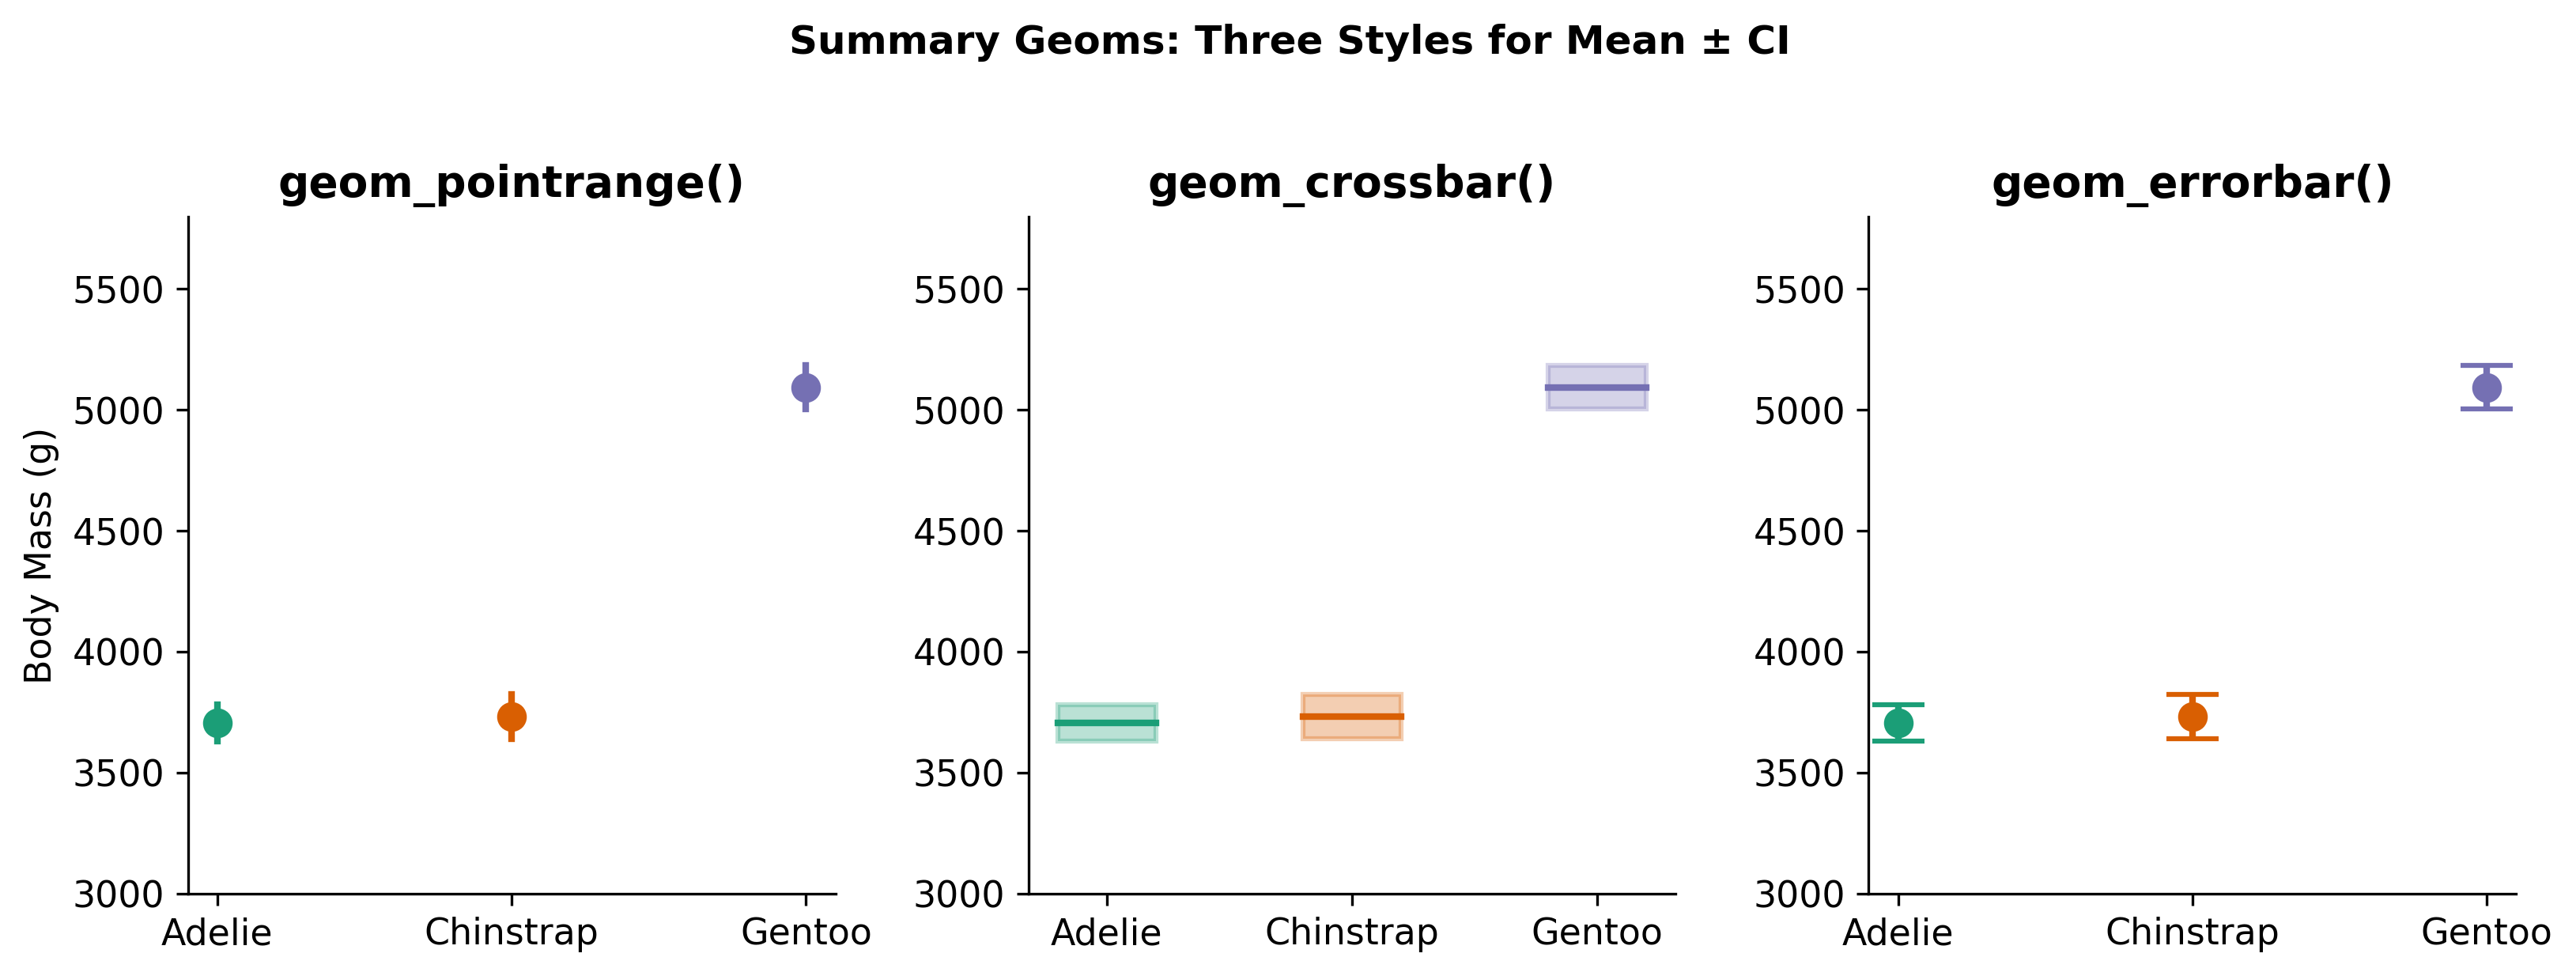
\includegraphics[width=\textwidth]{m2_1_summary_geoms.png}
\begin{exampleblock}{Data Insight}
    \scriptsize \texttt{sns.pointplot()} draws points connected by lines by default. Add \texttt{linestyle="none"} to get pure point + error bars without the connecting line.
\end{exampleblock}
\end{column}
\end{columns}
\end{frame}

% ── 16 ──
\begin{frame}{The Hybrid: Strip + Boxplot + Mean}
\smark{16/300}
\centering
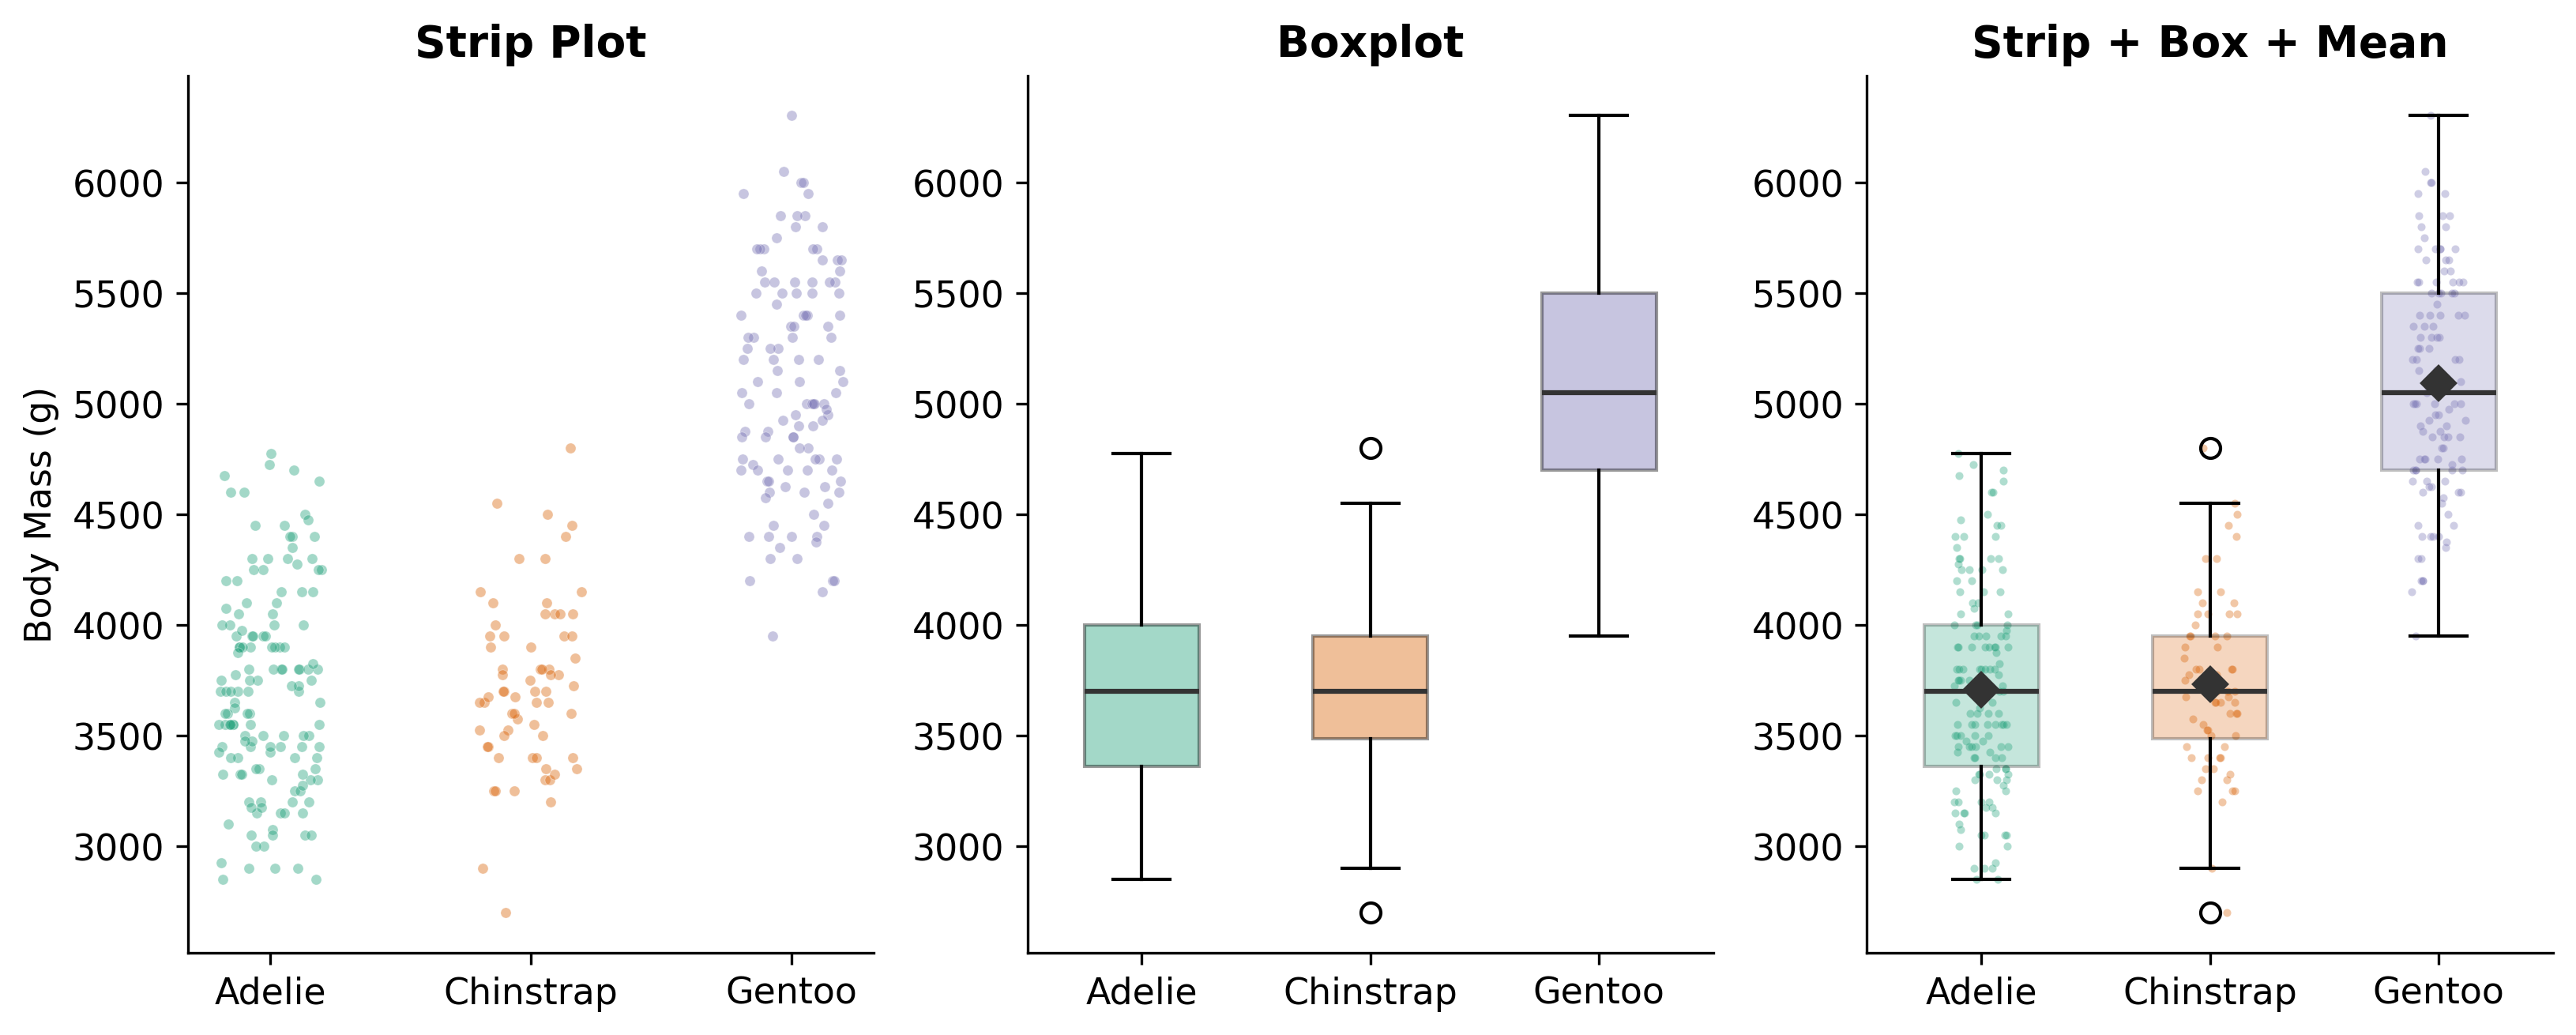
\includegraphics[width=0.88\textwidth]{m2_1_strip_box_mean.png}

\vspace{0.2cm}
\begin{exampleblock}{Data Insight}
    \scriptsize The \textbf{gold standard} for small-to-medium $n$: jittered raw points show every observation, the boxplot summarizes quartiles and IQR, and the diamond marks the mean. Three layers, maximum information.
\end{exampleblock}
\end{frame}

% ── 17 ──
\begin{frame}[fragile]{Hybrid Plot --- \Rlang}\smark{17/300}
\begin{columns}[T]
\begin{column}{0.55\textwidth}
\begin{lstlisting}[style=Rstyle]
ggplot(penguins,
  aes(species, body_mass_g,
      fill = species)) +
  # Layer 1: boxplot (light)
  geom_boxplot(alpha=0.25,
    outlier.shape=NA, width=0.5)+
  # Layer 2: strip (jittered)
  geom_jitter(aes(color=species),
    width=0.15, alpha=0.4,
    size=1) +
  # Layer 3: mean diamond
  stat_summary(fun=mean,
    geom="point", shape=18,
    size=4, color="black") +
  theme_minimal() +
  theme(legend.position="none")
\end{lstlisting}
\end{column}
\begin{column}{0.42\textwidth}
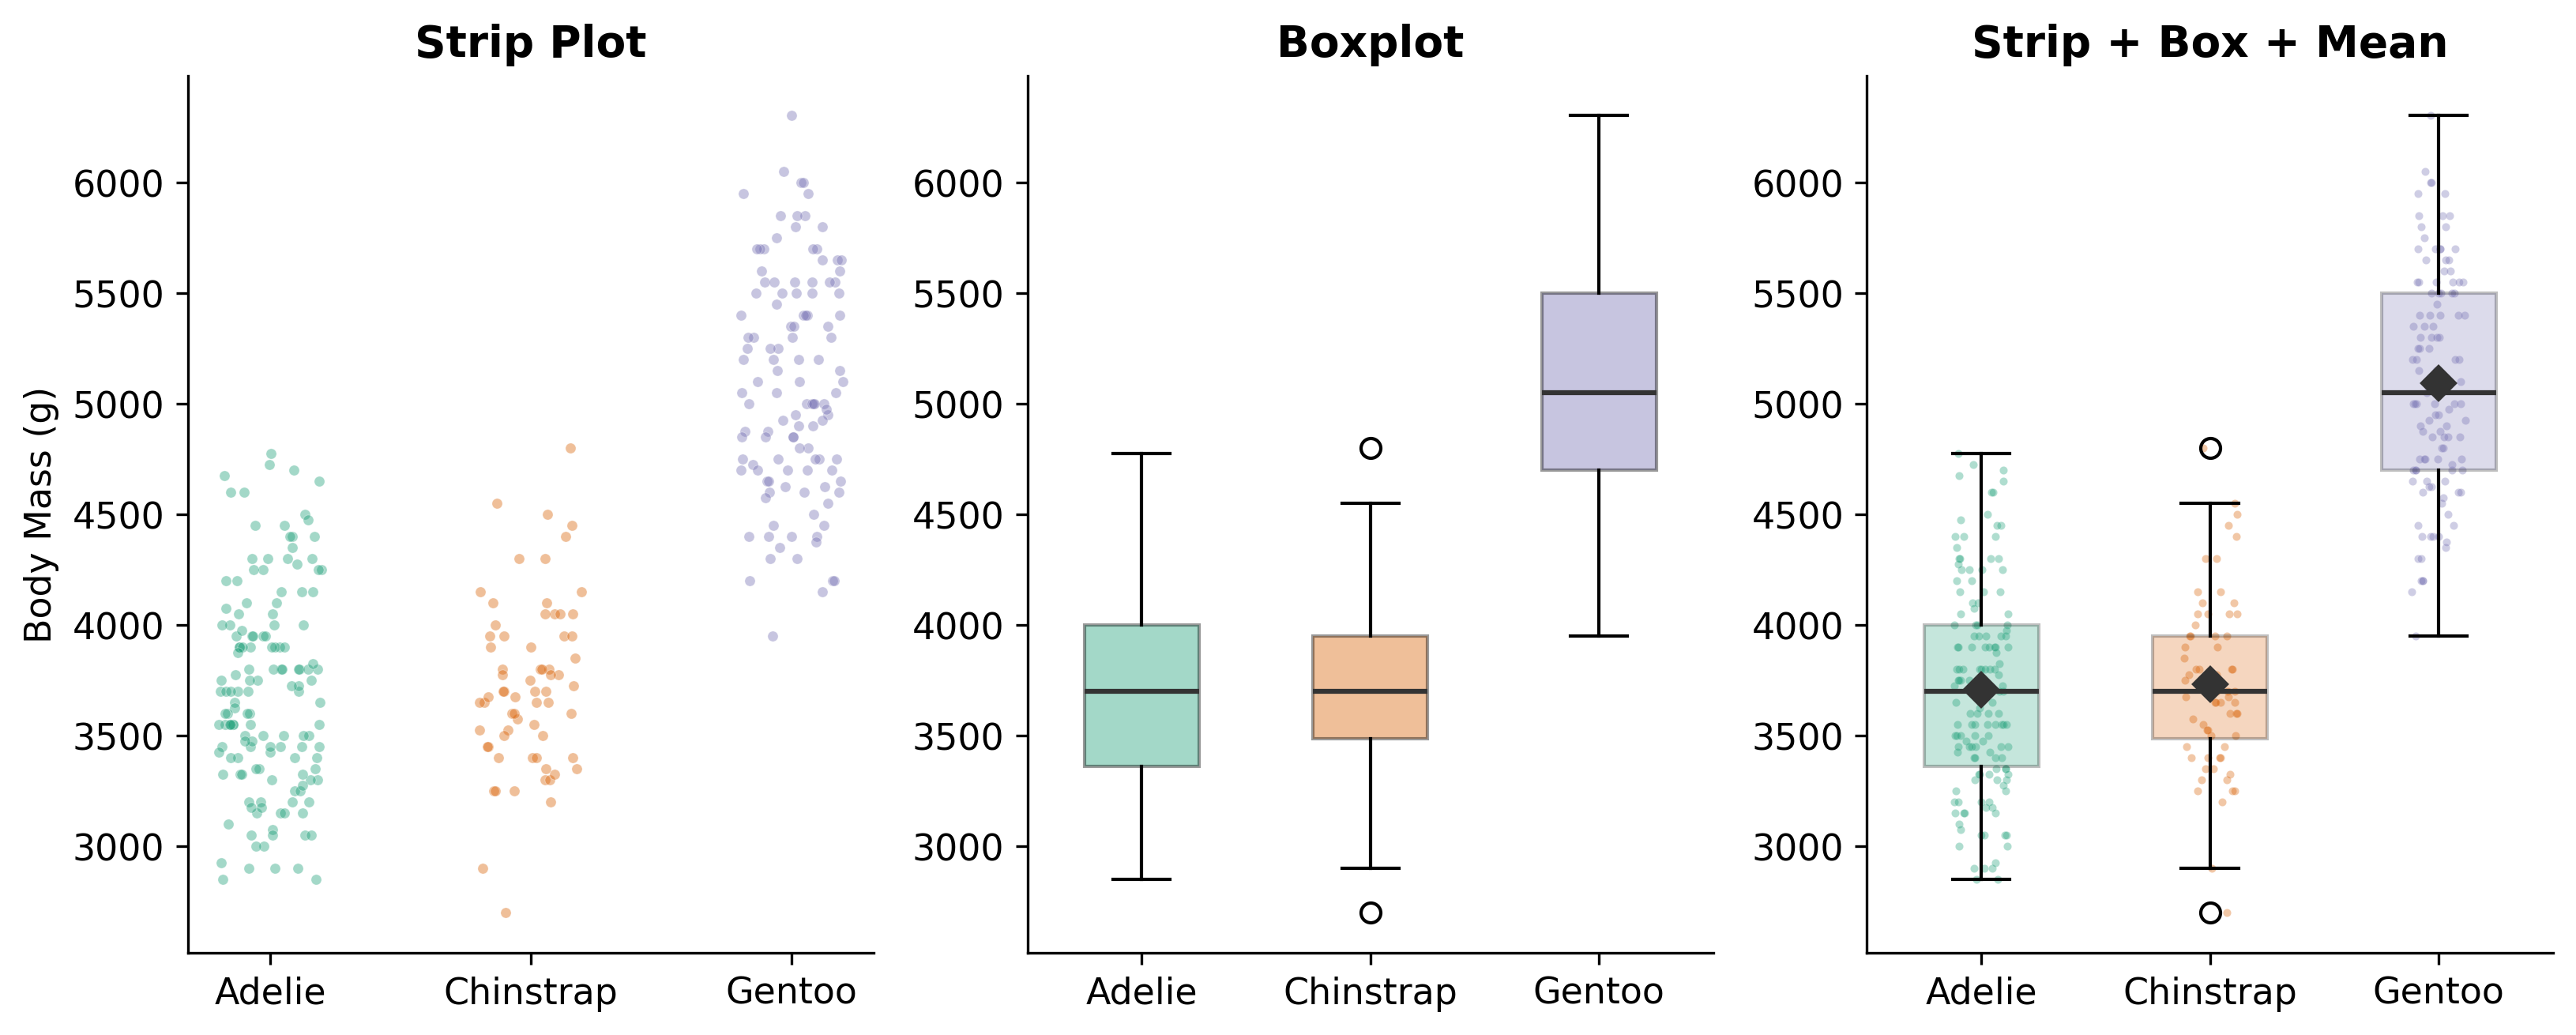
\includegraphics[width=\textwidth]{m2_1_strip_box_mean.png}
\begin{alertblock}{Pro-Tip}
    \scriptsize \texttt{outlier.shape=NA} hides boxplot outlier dots --- they would duplicate the jittered points. Layer order matters: box behind, points on top, mean diamond last.
\end{alertblock}
\end{column}
\end{columns}
\end{frame}

% ── 18 ──
\begin{frame}[fragile]{Hybrid Plot --- \Python}\smark{18/300}
\begin{columns}[T]
\begin{column}{0.55\textwidth}
\begin{lstlisting}[style=Pystyle]
fig, ax = plt.subplots()

# Layer 1: boxplot
sns.boxplot(data=penguins,
    x="species", y="body_mass_g",
    showfliers=False, width=0.5,
    palette=D, boxprops=dict(
        alpha=0.25), ax=ax)

# Layer 2: strip
sns.stripplot(data=penguins,
    x="species", y="body_mass_g",
    jitter=0.15, alpha=0.4, s=3,
    hue="species", legend=False,
    palette=D, ax=ax)

# Layer 3: mean diamond
means = penguins.groupby("species")\
    ["body_mass_g"].mean()
ax.scatter(range(3), means,
    marker="D", s=80, color="black",
    zorder=5)
\end{lstlisting}
\end{column}
\begin{column}{0.42\textwidth}
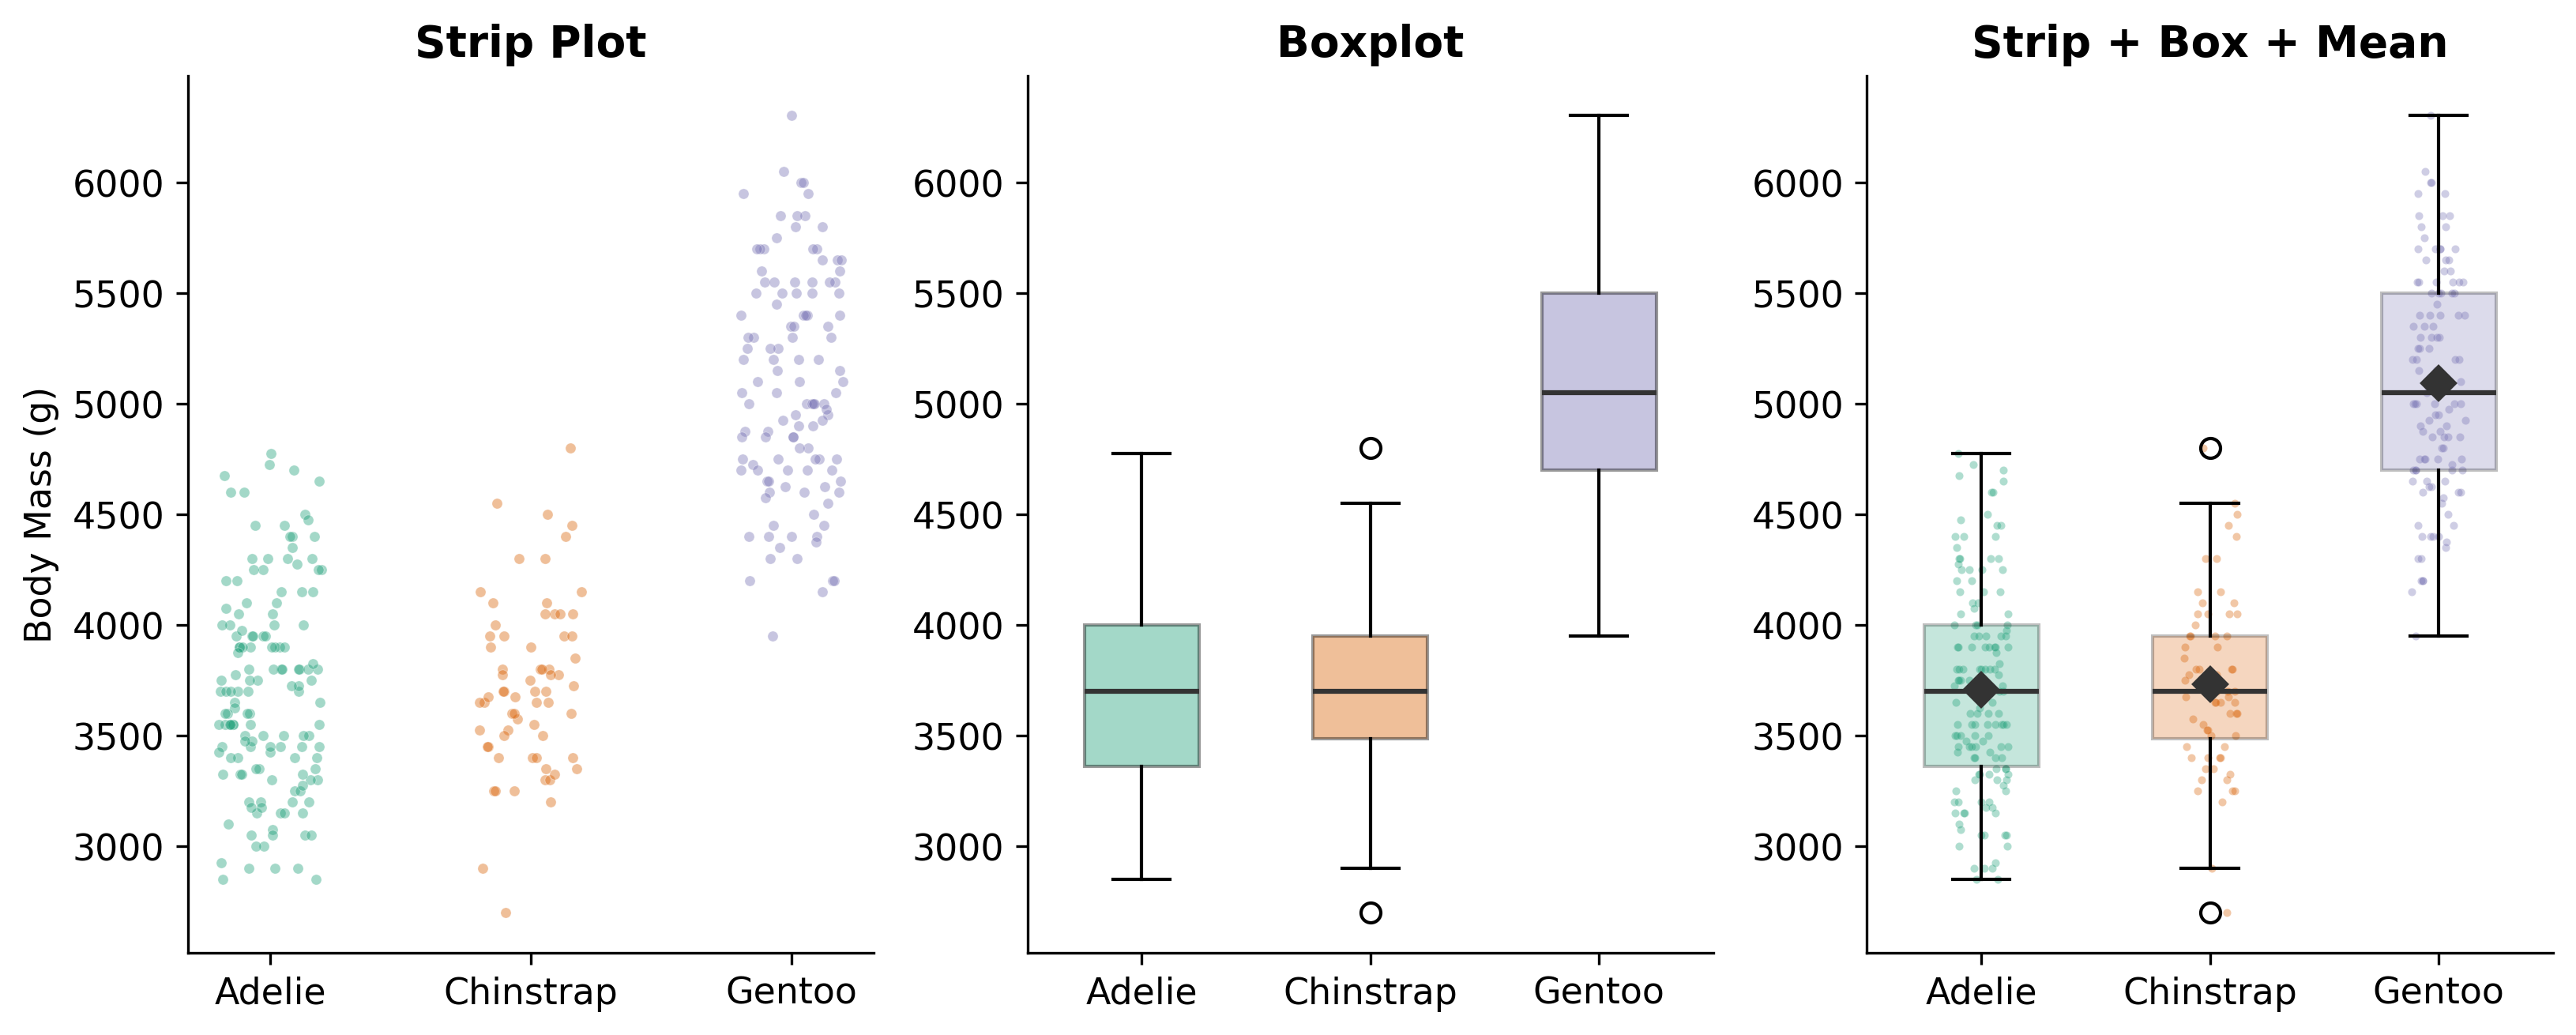
\includegraphics[width=\textwidth]{m2_1_strip_box_mean.png}
\begin{exampleblock}{Data Insight}
    \scriptsize \texttt{showfliers=False} in seaborn's \texttt{boxplot()} hides the built-in outlier markers. The strip plot already shows them.
\end{exampleblock}
\end{column}
\end{columns}
\end{frame}

% ── 19 ──
\begin{frame}{Bootstrap Confidence Intervals}
\smark{19/300}
\begin{columns}[T]
\begin{column}{0.50\textwidth}
\begin{itemize}
    \item Resample with replacement $B$ times ($B \geq 2{,}000$)
    \item Compute the statistic (e.g., mean) for each resample
    \item The 2.5th and 97.5th percentiles form the 95\% CI
    \item \textbf{No normality assumption} required
    \item Works for any statistic: median, ratio, correlation
\end{itemize}
\end{column}
\begin{column}{0.47\textwidth}
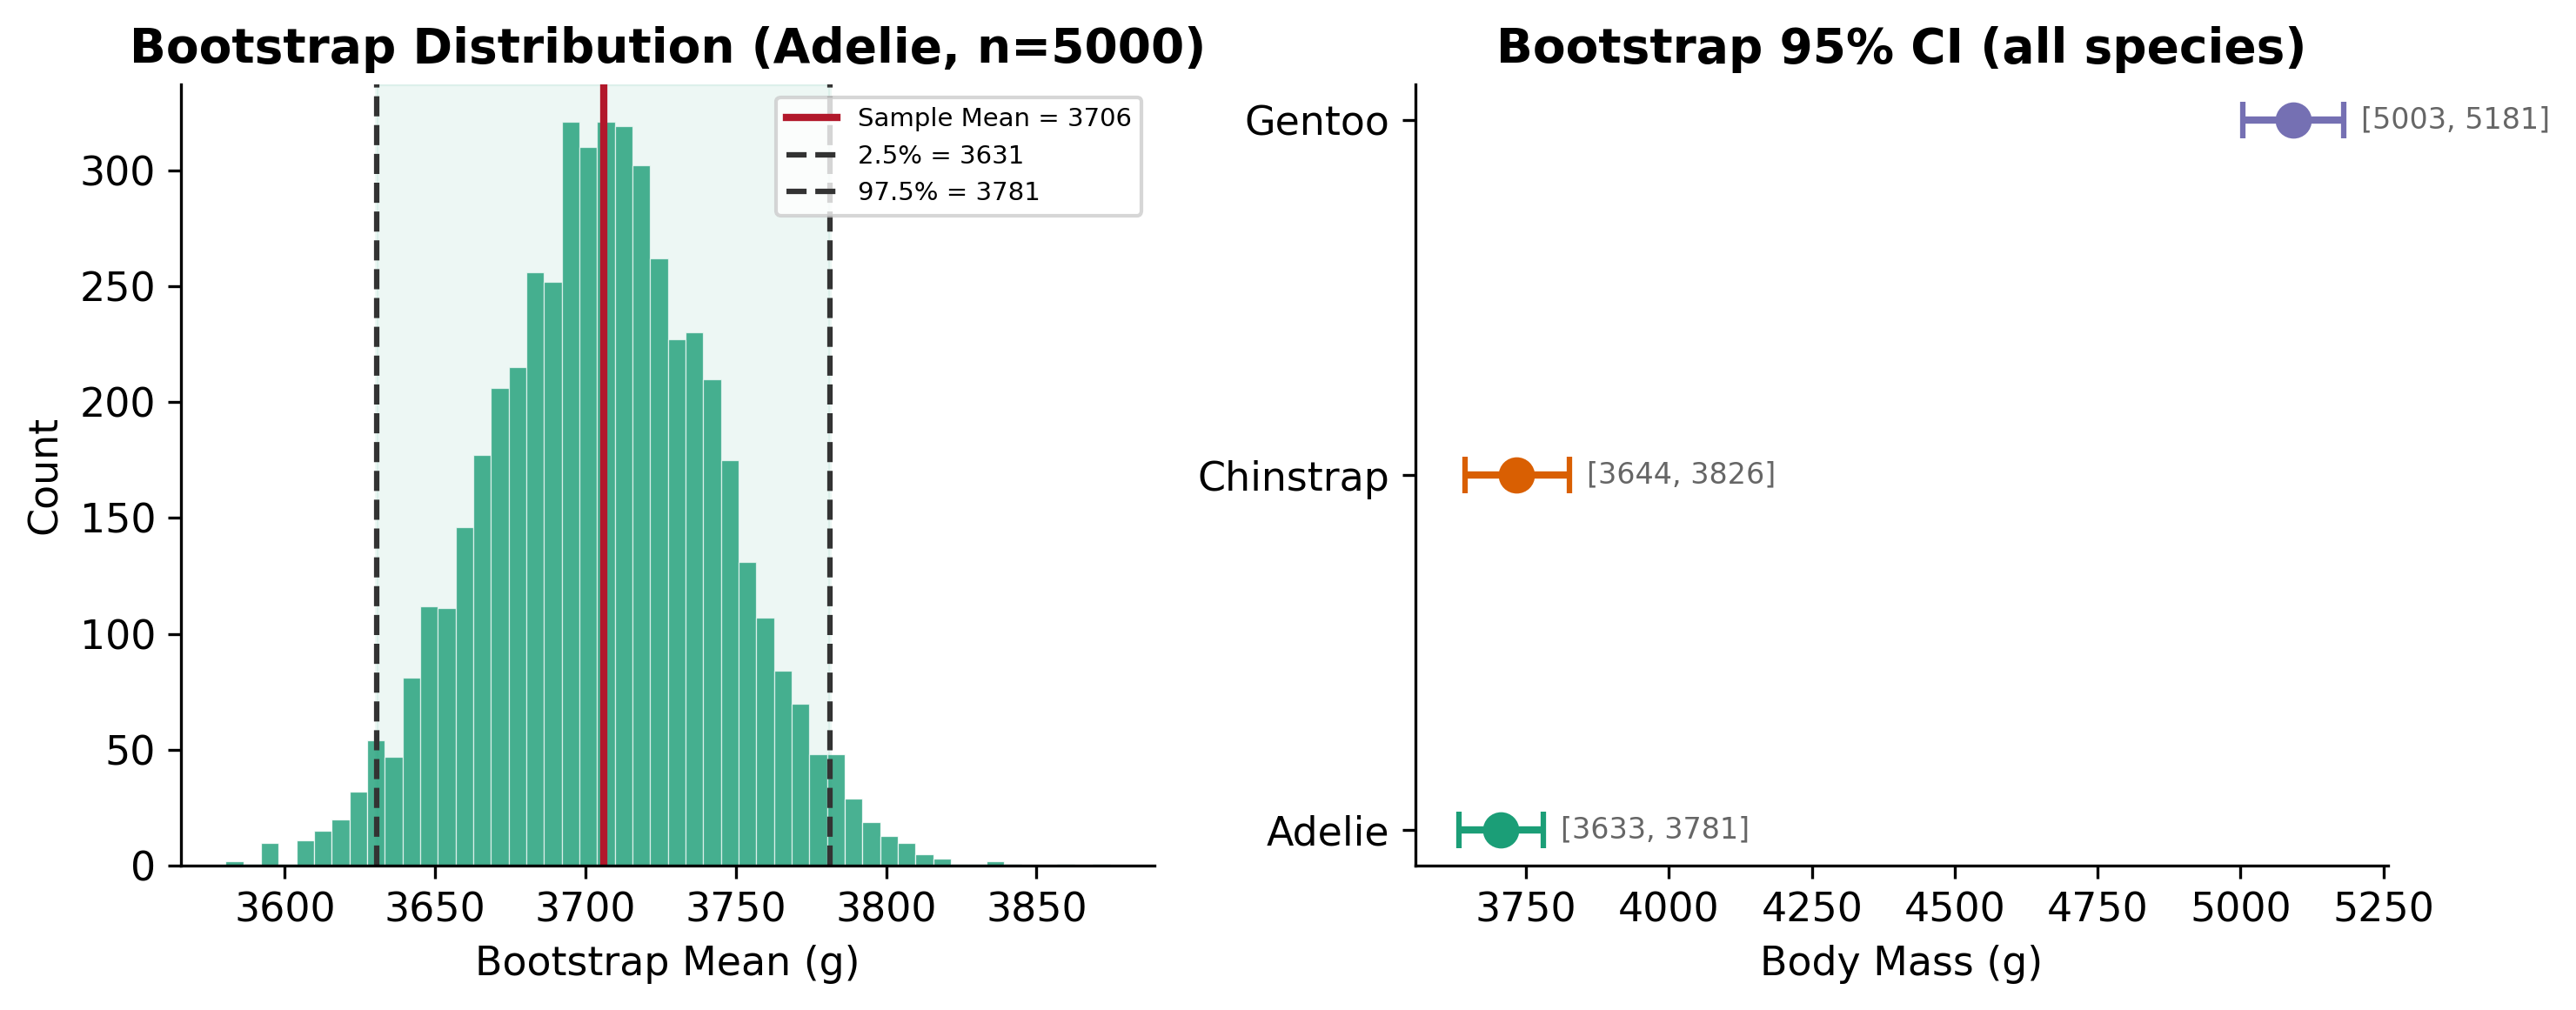
\includegraphics[width=\textwidth]{m2_1_bootstrap.png}
\begin{exampleblock}{Data Insight}
    \scriptsize The bootstrap distribution (left) approximates the sampling distribution of the mean. Its spread directly encodes uncertainty --- wider = less precise.
\end{exampleblock}
\end{column}
\end{columns}
\end{frame}

% ── 20 ──
\begin{frame}[fragile]{Bootstrap CI --- \Rlang}\smark{20/300}
\begin{columns}[T]
\begin{column}{0.55\textwidth}
\begin{lstlisting}[style=Rstyle]
# Hmisc within stat_summary
ggplot(penguins,
  aes(species, body_mass_g)) +
  stat_summary(
    fun.data = mean_cl_boot,
    geom = "pointrange",
    color = "#2166AC") +
  theme_minimal()

# Manual bootstrap
library(boot)
boot_fn <- function(d, i)
  mean(d[i])
b <- boot(adelie_mass,
  boot_fn, R=5000)
boot.ci(b, type="perc")
\end{lstlisting}
\end{column}
\begin{column}{0.42\textwidth}
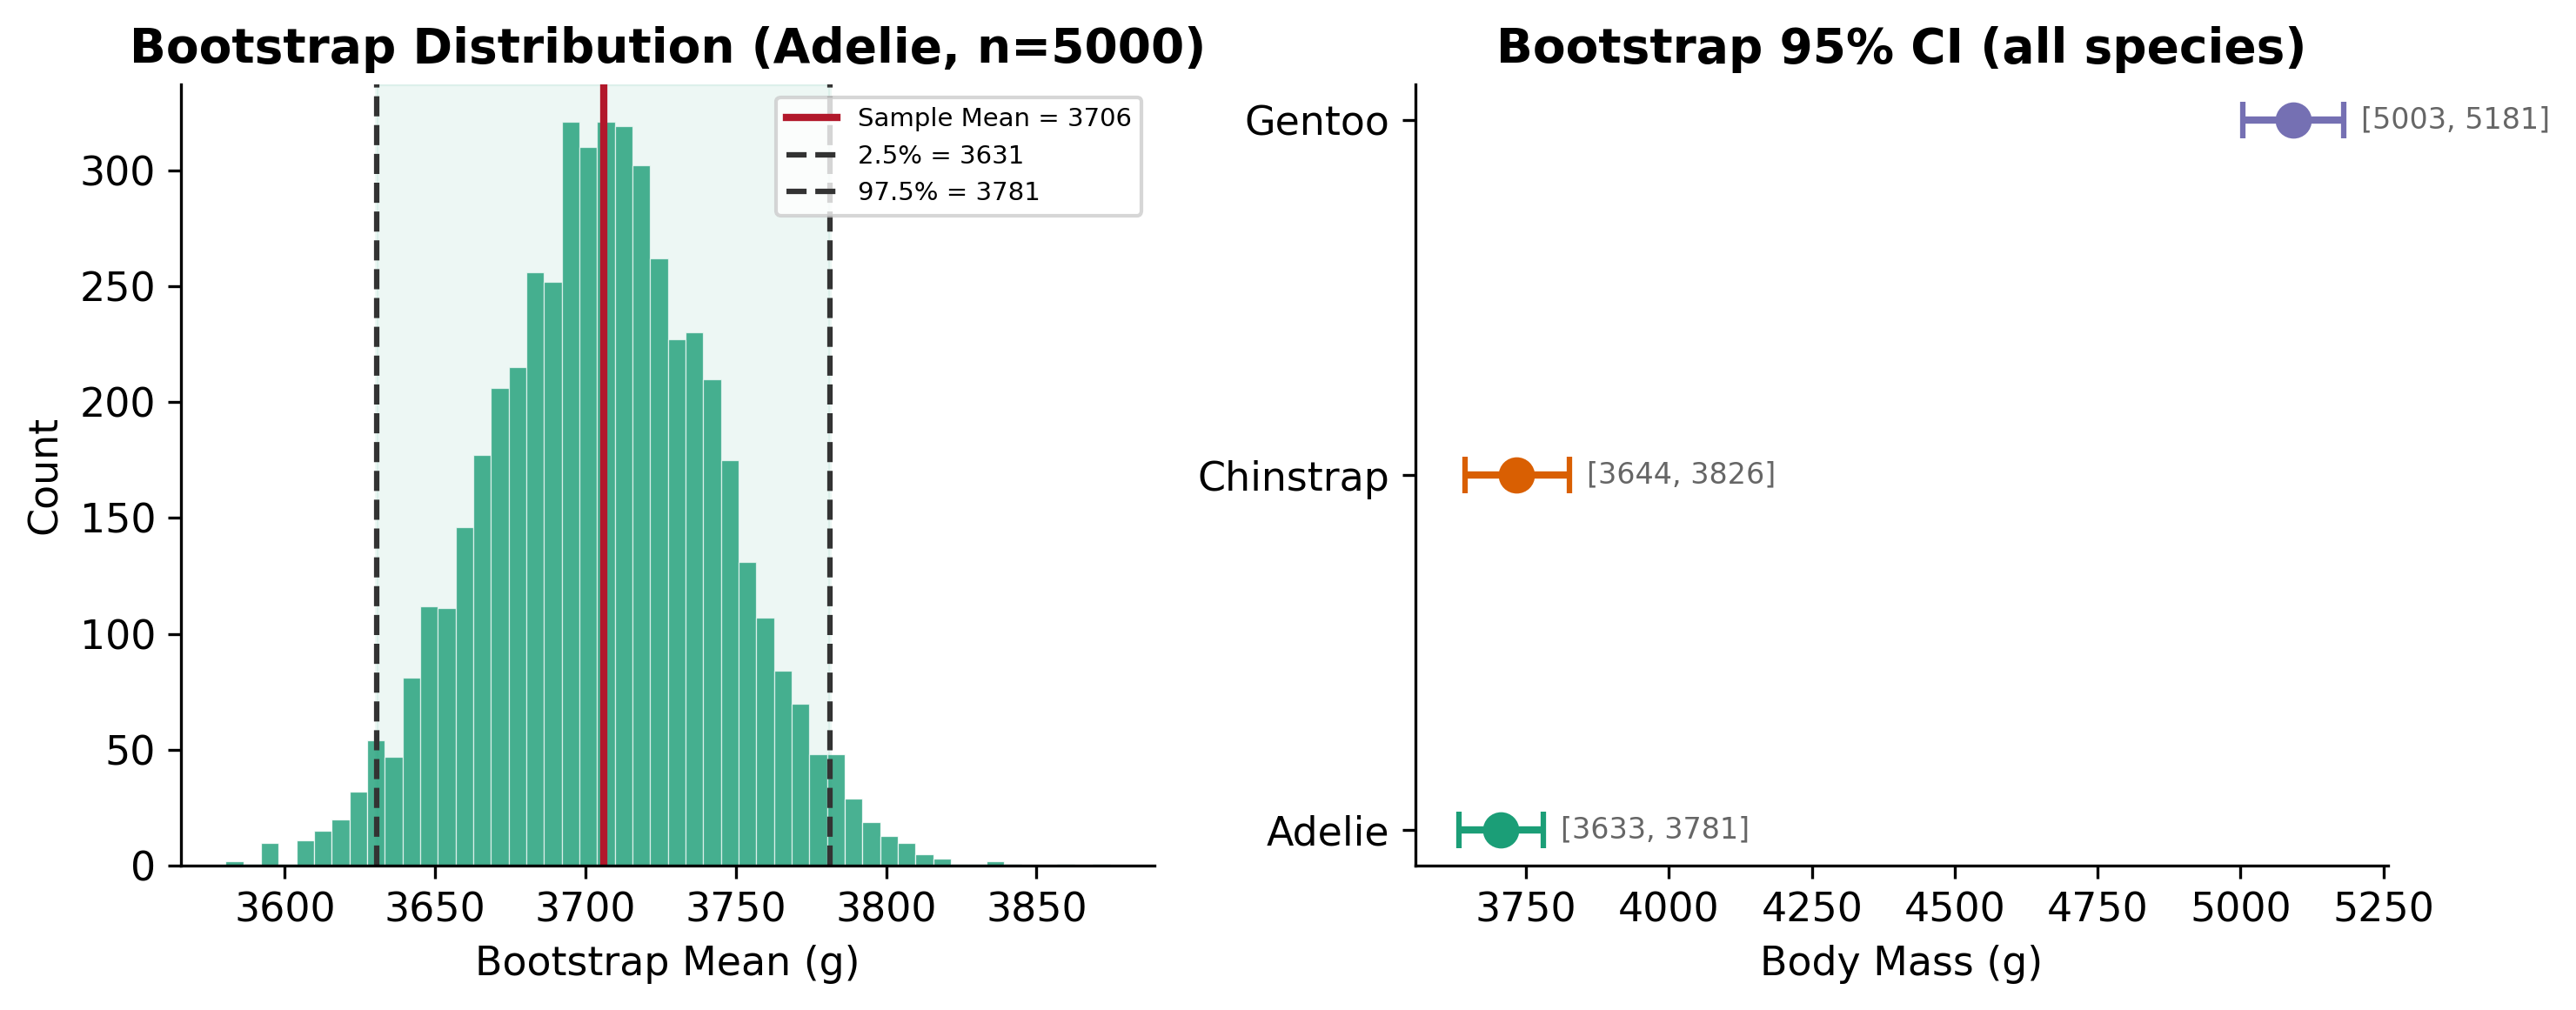
\includegraphics[width=\textwidth]{m2_1_bootstrap.png}
\begin{alertblock}{Pro-Tip}
    \scriptsize \texttt{mean\_cl\_boot} inside \texttt{stat\_summary()} handles the bootstrap internally. For custom statistics, use the \texttt{boot} package directly.
\end{alertblock}
\end{column}
\end{columns}
\end{frame}

% ── 21 ──
\begin{frame}[fragile]{Bootstrap CI --- \Python}\smark{21/300}
\begin{columns}[T]
\begin{column}{0.55\textwidth}
\begin{lstlisting}[style=Pystyle]
from scipy.stats import bootstrap

# Per-species bootstrap
for sp in species_list:
    data = (pen.query(
        f"species=='{sp}'")
        ["body_mass_g"].values,)
    res = bootstrap(data, np.mean,
        n_resamples=5000,
        confidence_level=0.95)
    lo = res.confidence_interval.low
    hi = res.confidence_interval.high
    print(f"{sp}: [{lo:.0f}, {hi:.0f}]")

# seaborn auto-bootstrap
sns.pointplot(data=penguins,
    x="species", y="body_mass_g",
    errorbar=("ci", 95))
\end{lstlisting}
\end{column}
\begin{column}{0.42\textwidth}
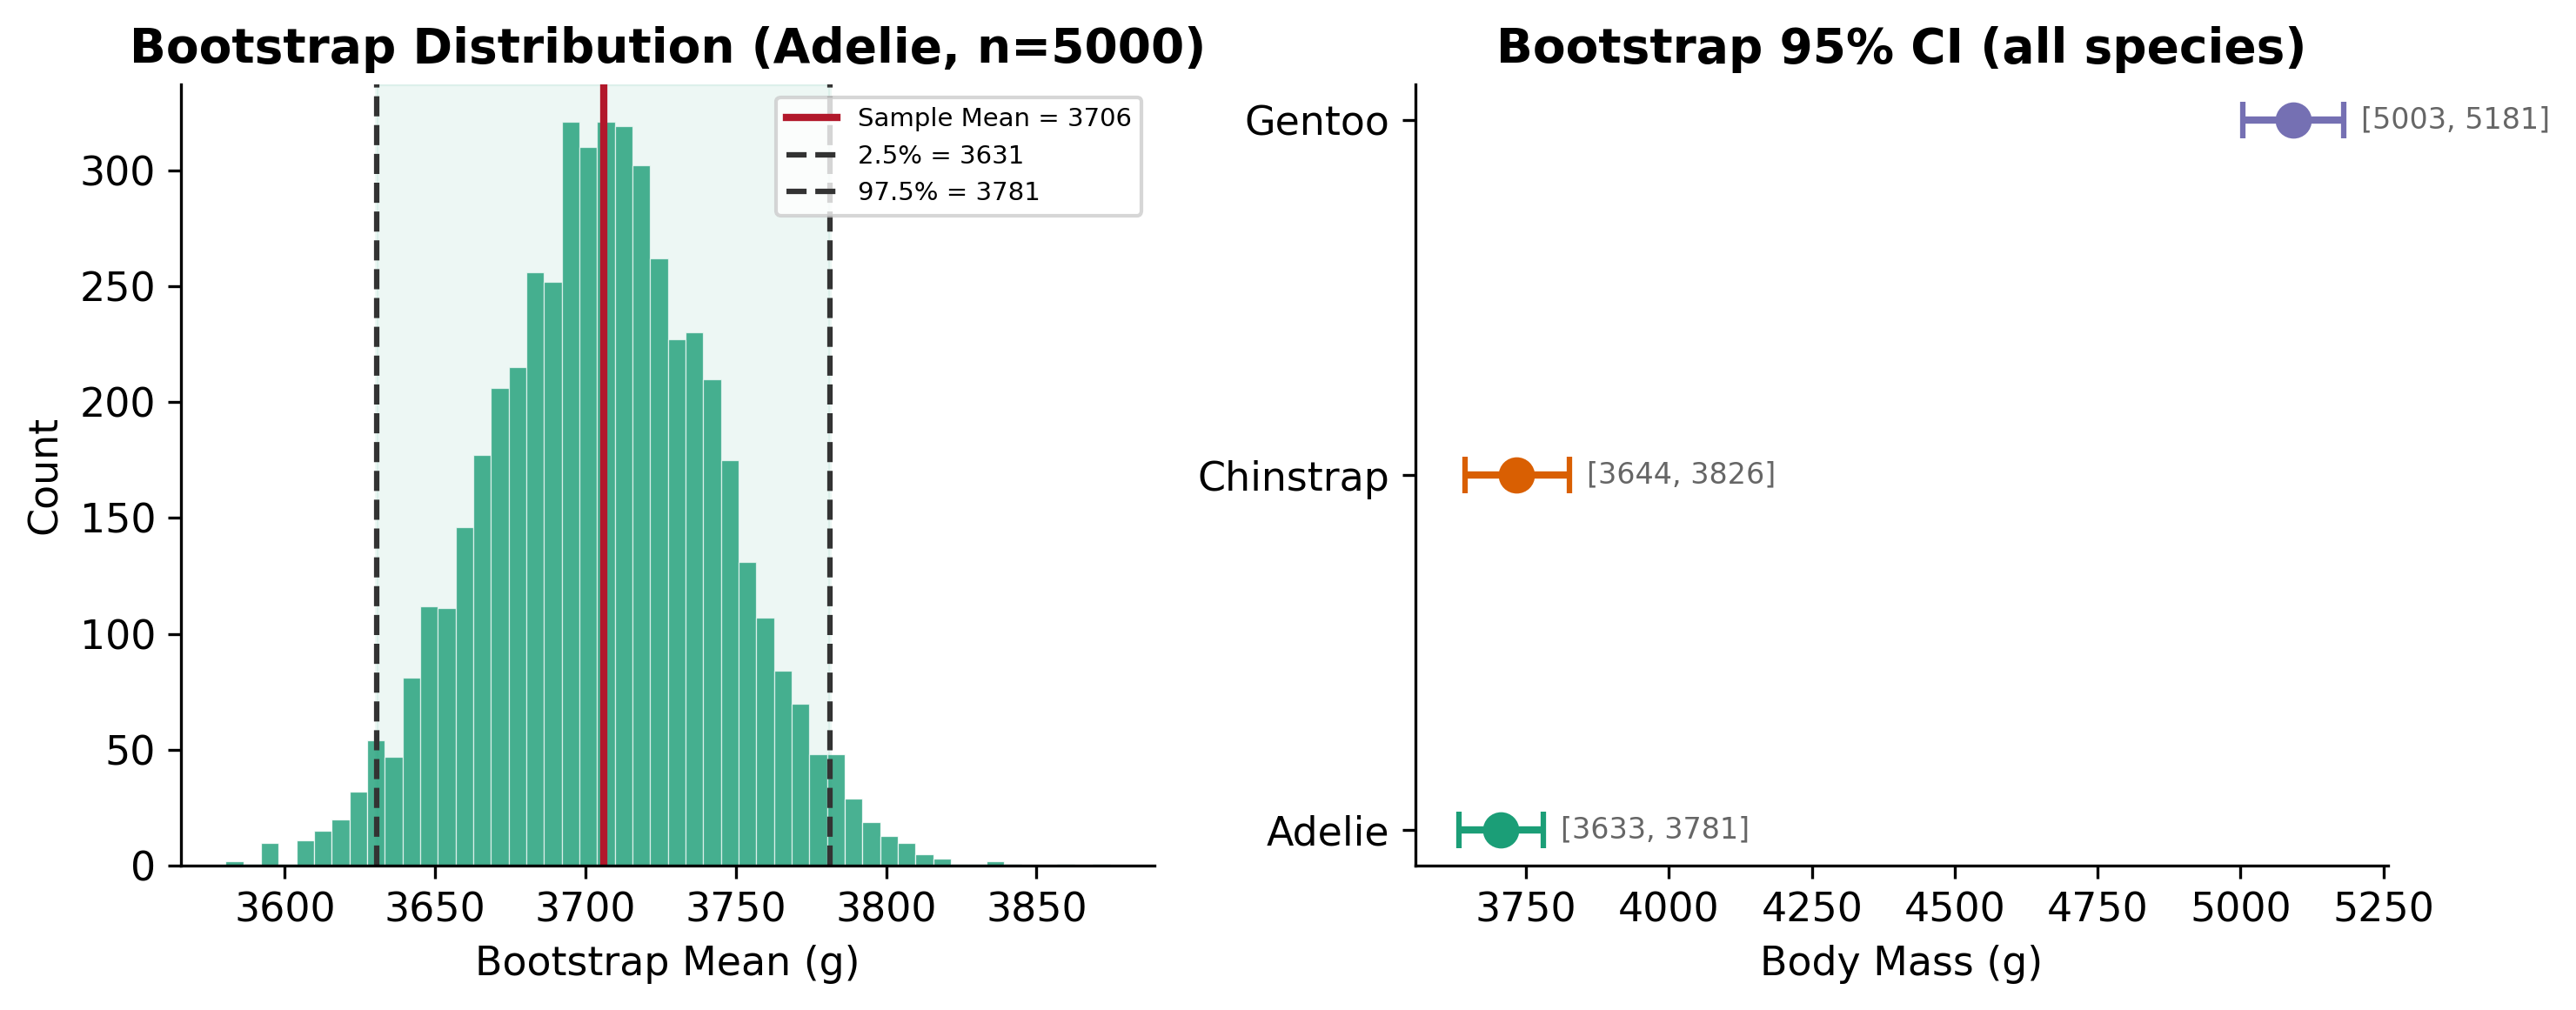
\includegraphics[width=\textwidth]{m2_1_bootstrap.png}
\begin{exampleblock}{Data Insight}
    \scriptsize seaborn's \texttt{errorbar=("ci", 95)} runs a bootstrap internally. For full control, use \texttt{scipy.stats.bootstrap()} and plot manually.
\end{exampleblock}
\end{column}
\end{columns}
\end{frame}

% ── 22 ──
\begin{frame}{Cleveland Dot Plot for Ranked Comparisons}
\smark{22/300}
\centering
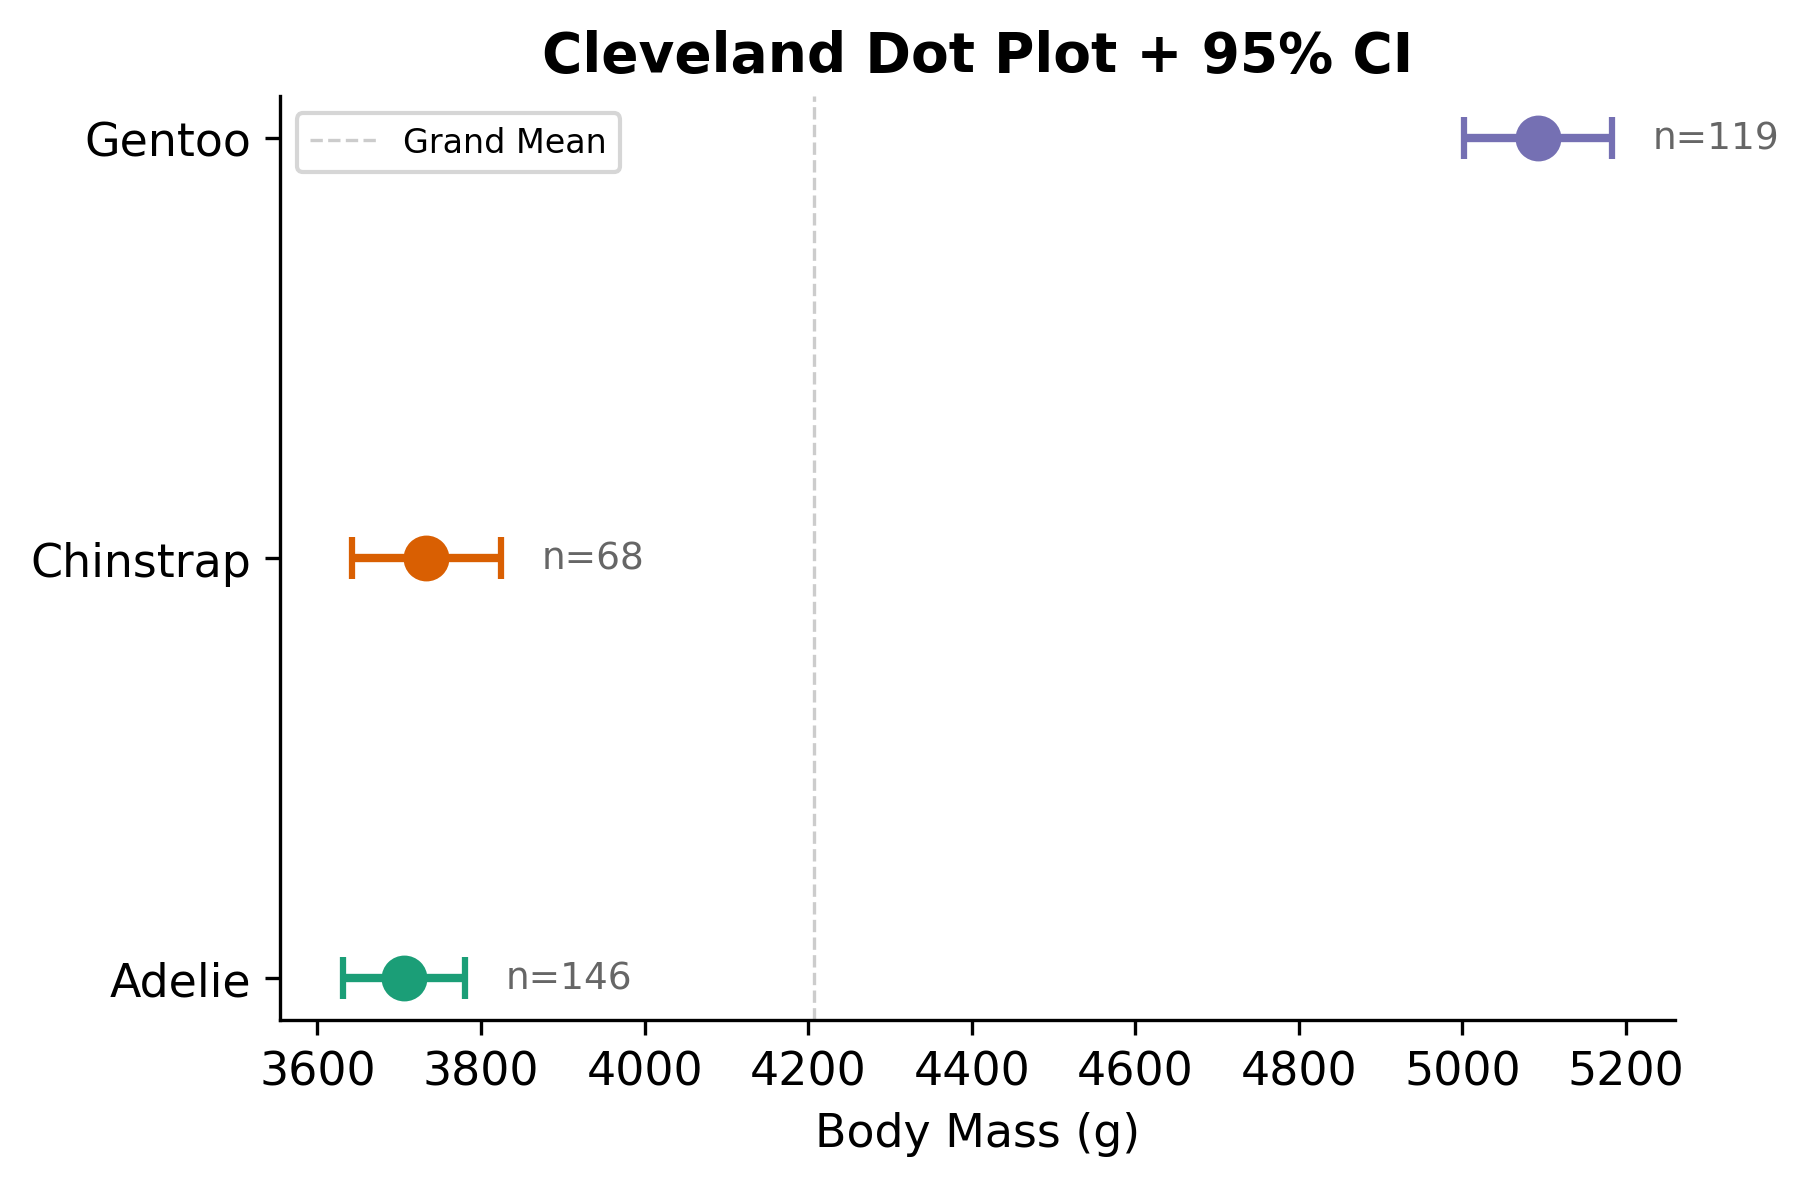
\includegraphics[width=0.62\textwidth]{m2_1_dotplot_ci.png}

\vspace{0.2cm}
\begin{columns}[T]
\begin{column}{0.48\textwidth}
\begin{itemize}
    \item Horizontal point + CI for each group
    \item Sorted by value (largest at top)
    \item Grand mean as reference line
    \item Better than grouped bar chart for ranked comparisons
\end{itemize}
\end{column}
\begin{column}{0.48\textwidth}
\begin{exampleblock}{Data Insight}
    \scriptsize Cleveland (1984): the dot plot uses \textbf{position on a common scale} (rank 1 encoding) vs.\ bars which use \textbf{length} (rank 3). Dot plots are perceptually superior for group comparison.
\end{exampleblock}
\end{column}
\end{columns}
\end{frame}

% ── 23 ──
\begin{frame}[fragile]{Cleveland Dot Plot --- \Rlang}\smark{23/300}
\begin{columns}[T]
\begin{column}{0.55\textwidth}
\begin{lstlisting}[style=Rstyle]
# Compute summary
summ <- penguins |>
  group_by(species) |>
  summarise(
    m  = mean(body_mass_g),
    se = sd(body_mass_g) /
         sqrt(n()),
    lo = m - 1.96*se,
    hi = m + 1.96*se)

ggplot(summ,
  aes(m, fct_reorder(species, m)))+
  geom_pointrange(
    aes(xmin=lo, xmax=hi),
    color="#2166AC", size=0.8) +
  geom_vline(xintercept =
    mean(penguins$body_mass_g),
    linetype="dashed", color="#CCC")+
  labs(x="Body Mass (g)", y=NULL) +
  theme_minimal()
\end{lstlisting}
\end{column}
\begin{column}{0.42\textwidth}
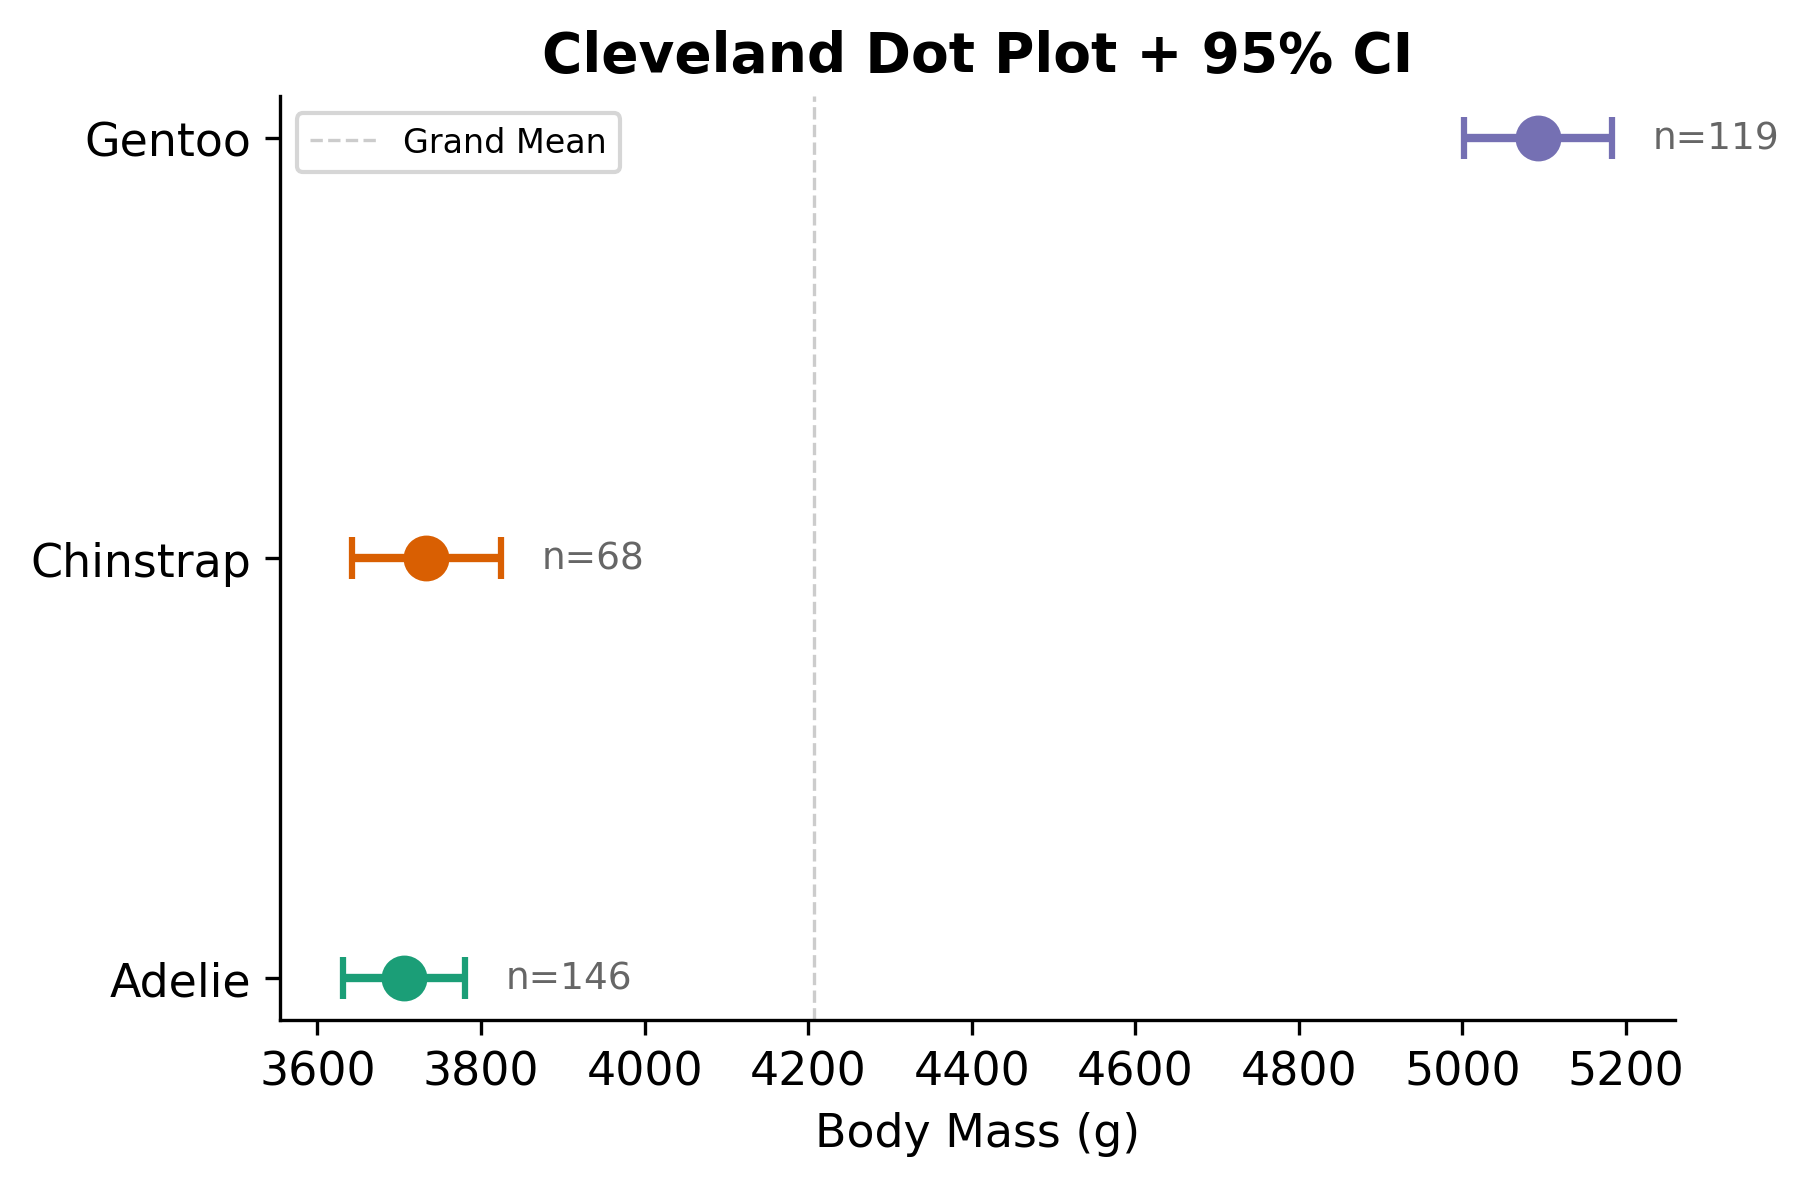
\includegraphics[width=\textwidth]{m2_1_dotplot_ci.png}
\begin{alertblock}{Pro-Tip}
    \scriptsize \texttt{geom\_pointrange(aes(xmin=, xmax=))} creates horizontal intervals. \texttt{fct\_reorder(species, m)} sorts species by their mean.
\end{alertblock}
\end{column}
\end{columns}
\end{frame}

% ── 24 ──
\begin{frame}[fragile]{Cleveland Dot Plot --- \Python}\smark{24/300}
\begin{columns}[T]
\begin{column}{0.55\textwidth}
\begin{lstlisting}[style=Pystyle]
summ = penguins.groupby("species")\
    ["body_mass_g"].agg(
    ["mean","sem"]).reset_index()
summ["lo"] = summ["mean"]-1.96*summ["sem"]
summ["hi"] = summ["mean"]+1.96*summ["sem"]
summ = summ.sort_values("mean")

fig, ax = plt.subplots(figsize=(6,3))
for i, row in summ.iterrows():
    ax.errorbar(row["mean"], row["species"],
        xerr=[[row["mean"]-row["lo"]],
              [row["hi"]-row["mean"]]],
        fmt="o", capsize=5, color=B,
        markersize=9, linewidth=2)
ax.axvline(penguins["body_mass_g"].mean(),
    linestyle="--", color="#CCC")
ax.set_xlabel("Body Mass (g)")
\end{lstlisting}
\end{column}
\begin{column}{0.42\textwidth}
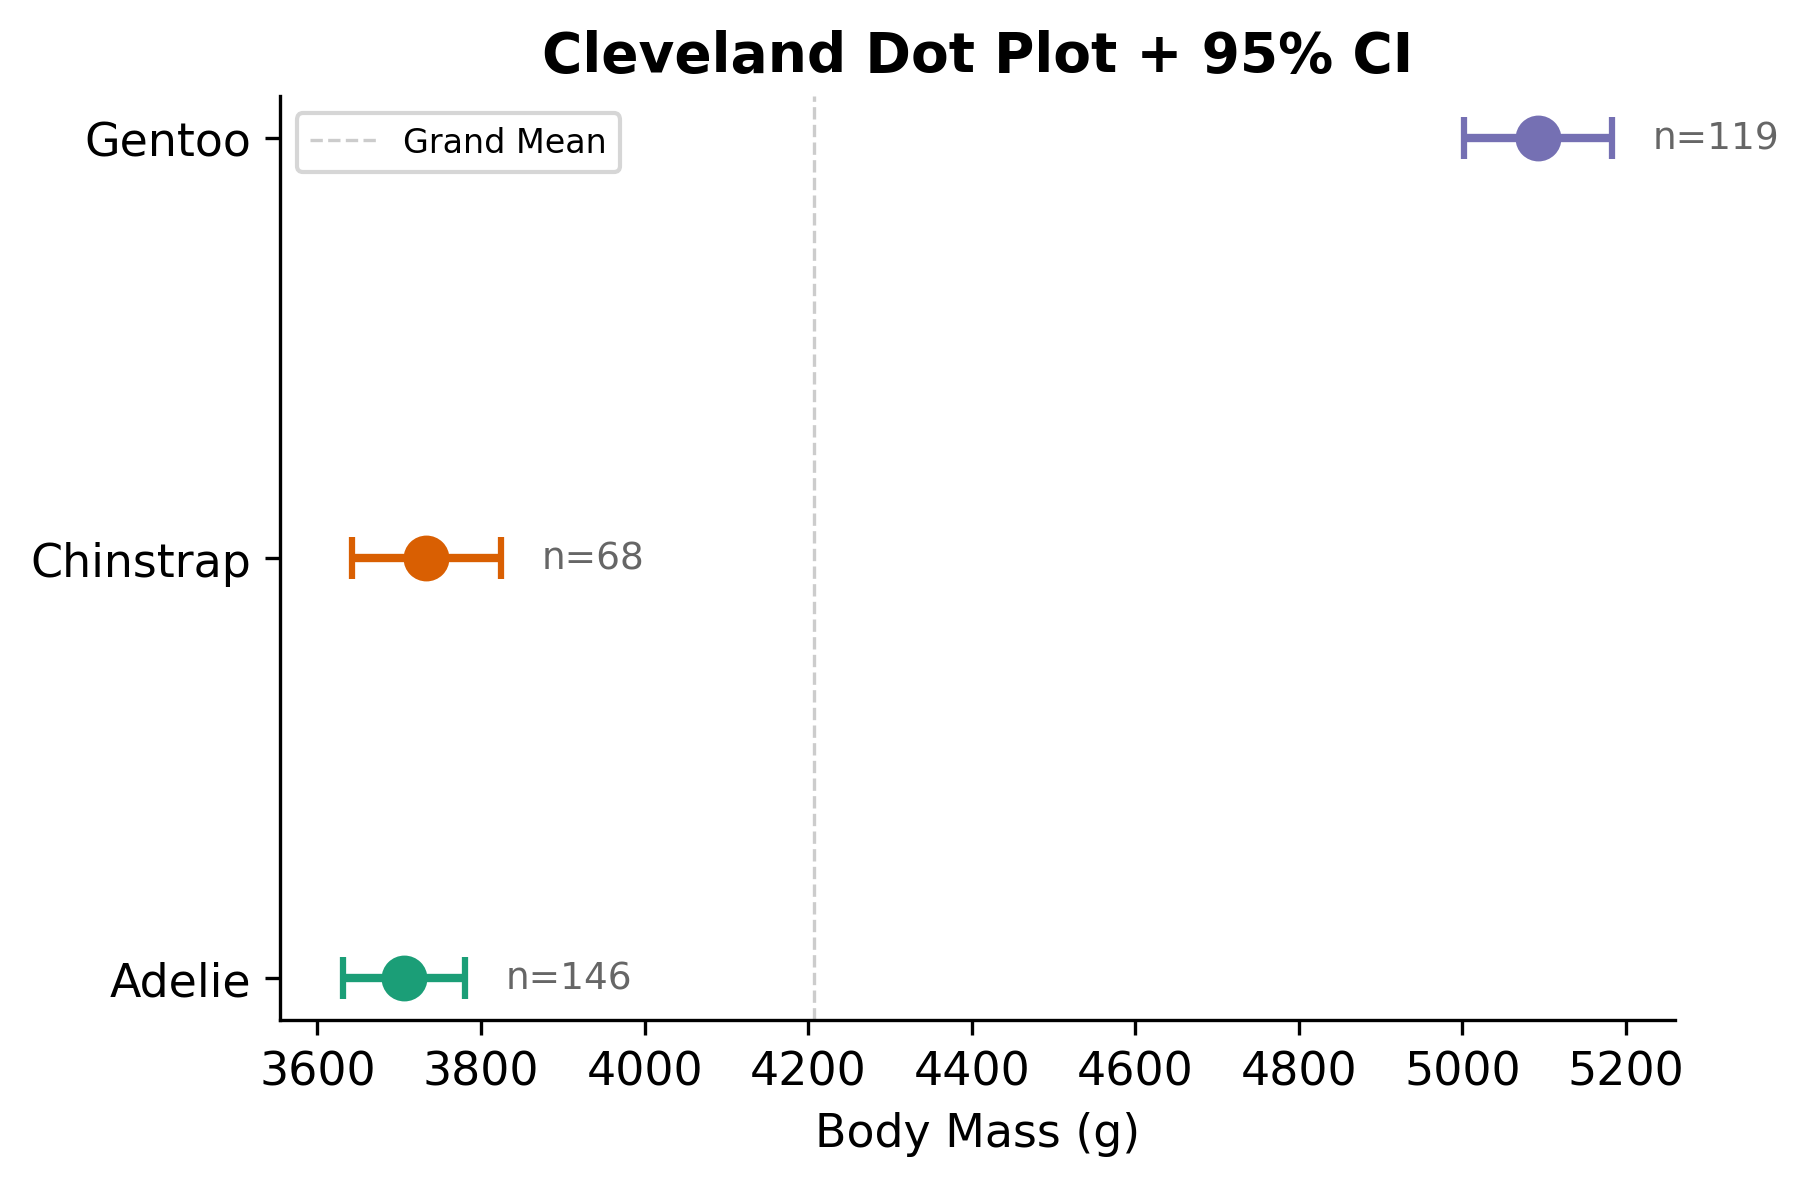
\includegraphics[width=\textwidth]{m2_1_dotplot_ci.png}
\end{column}
\end{columns}
\end{frame}

% ── 25 ──
\begin{frame}{\texttt{stat\_summary()}: The Swiss Army Knife}
\smark{25/300}
\centering\small
\begin{tabular}{@{}lll@{}}
    \toprule
    \textbf{fun.data =} & \textbf{Returns} & \textbf{Package} \\
    \midrule
    \texttt{mean\_se}       & $\bar{x} \pm \text{SE}$                & ggplot2 (built-in) \\
    \texttt{mean\_cl\_boot}  & Bootstrap 95\% CI                       & Hmisc \\
    \texttt{mean\_cl\_normal}& Normal-theory 95\% CI                   & Hmisc \\
    \texttt{mean\_sdl}      & $\bar{x} \pm k \cdot \text{SD}$         & Hmisc \\
    \texttt{median\_hilow}  & Median + quantile range                  & Hmisc \\
    Custom function          & Any \texttt{data.frame(y, ymin, ymax)}  & User-defined \\
    \bottomrule
\end{tabular}

\vspace{0.3cm}
\begin{exampleblock}{Data Insight}
    \scriptsize \texttt{stat\_summary()} computes the summary \textbf{inside} ggplot2 --- no manual aggregation needed. Combine with any geom: \texttt{pointrange}, \texttt{crossbar}, \texttt{errorbar}, \texttt{linerange}.
\end{exampleblock}
\end{frame}

% ── 26 ──
\begin{frame}{When to Show Raw Data vs.\ Summary Only}
\smark{26/300}
\centering\small
\begin{tabular}{@{}lll@{}}
    \toprule
    \textbf{$n$ per group} & \textbf{Recommendation} & \textbf{Why} \\
    \midrule
    $n < 10$    & Raw points only (no box/violin)          & Too few for summary stats \\
    $10 \leq n \leq 50$  & Strip + box or strip + mean $\pm$ CI & Show data + summary \\
    $50 < n \leq 200$ & Violin + box or raincloud          & Strip becomes dense \\
    $n > 200$   & Violin or density + mean $\pm$ CI        & Points overplot completely \\
    \bottomrule
\end{tabular}

\vspace{0.3cm}
\begin{alertblock}{Pro-Tip}
    \scriptsize The decision depends on $n$ \textbf{per group}, not total $n$. If you have 3 species with $n=150$ each, violin + box is appropriate. If one group has $n=8$, show its raw points.
\end{alertblock}
\end{frame}

% ── 27 ──
\begin{frame}{Paired Data: Before/After Comparisons}
\smark{27/300}
\begin{columns}[T]
\begin{column}{0.50\textwidth}
\begin{itemize}
    \item Connect matched observations with lines
    \item Slope of each line = individual change
    \item Upward lines $\to$ increase; downward $\to$ decrease
    \item The distribution of \textbf{slopes} is the effect
    \item More informative than two separate boxplots
\end{itemize}
\end{column}
\begin{column}{0.47\textwidth}
\begin{alertblock}{Pro-Tip}
    \scriptsize In ggplot2: \texttt{geom\_line(aes(group=subject\_id))} connects paired points. In seaborn: no built-in paired plot --- use matplotlib's \texttt{ax.plot()} with a loop over subjects.
\end{alertblock}
\vspace{0.2cm}
\begin{exampleblock}{Data Insight}
    \scriptsize If most lines slope upward but a few slope steeply down, the mean change may be positive but the \emph{mechanism} is heterogeneous. The lines reveal this; a bar of means hides it.
\end{exampleblock}
\end{column}
\end{columns}
\end{frame}

% ── 28 ──
\begin{frame}[fragile]{Paired Plot --- Code}\smark{28/300}
\begin{columns}[T]
\begin{column}{0.48\textwidth}
\begin{lstlisting}[style=Rstyle]
# Each line = one subject
ggplot(paired_df,
  aes(x = time, y = score,
      group = subject_id)) +
  geom_line(alpha = 0.3,
    color = "#999") +
  geom_point(aes(color = time),
    size = 2) +
  stat_summary(
    aes(group = 1),
    fun = mean,
    geom = "line",
    color = "#B2182B",
    linewidth = 1.5) +
  theme_minimal()
\end{lstlisting}
\end{column}
\begin{column}{0.48\textwidth}
\begin{lstlisting}[style=Pystyle]
# matplotlib paired lines
for _, row in df.iterrows():
    ax.plot([0, 1],
        [row["pre"], row["post"]],
        color="#CCC", alpha=0.3)

# Group means
ax.plot([0, 1],
    [df["pre"].mean(),
     df["post"].mean()],
    color="#B2182B",
    linewidth=2, marker="o")

ax.set_xticks([0, 1])
ax.set_xticklabels(
    ["Pre", "Post"])
\end{lstlisting}
\end{column}
\end{columns}
\end{frame}

% ── 29 ──
\begin{frame}{Module 2.1 --- Key Takeaways}\smark{29/300}
\begin{enumerate}
    \item \textbf{Ban the dynamite plot.} It hides everything that matters.
    \item \textbf{Show raw data} when $n$ permits (strip, jitter, beeswarm).
    \item \textbf{Label your error bars.} SE $\neq$ CI $\neq$ SD.
    \item \textbf{Hybrid plots} (strip + box + mean) maximize information density.
    \item \textbf{Bootstrap CIs} require no distributional assumptions.
    \item \textbf{Cleveland dot plots} outperform grouped bars for ranked comparisons.
\end{enumerate}
\end{frame}

% ── 30 ──  (slide number 31 counting title)
\begin{frame}{}\smark{31/300}
\centering\vspace{1.5cm}
{\Large\textbf{Module 2.1 Complete}}\\[0.5cm]
You can now replace dynamite plots with transparent, information-rich alternatives --- strip, hybrid, bootstrap, and Cleveland dot plots.\\[0.5cm]
\textbf{Next:} Module 2.2 --- Boxplots, Violins, Raincloud, and Beeswarm.
\end{frame}

% % ═══════════════════════════════════════════════════════
%  MODULE 2.2 — Boxplots, Violins, Raincloud, and Beeswarm
% ═══════════════════════════════════════════════════════
\section{Module 2.2 --- Boxplots, Violins, Raincloud, and Beeswarm}

% ── 32 ──
\begin{frame}{Module 2.2 --- Roadmap}\smark{32/300}
\begin{enumerate}
    \item Boxplot anatomy: quartiles, whiskers, outliers
    \item Boxplot limitations: hiding bimodality and $n$
    \item The violin plot: KDE turned on its side
    \item Violin + box + jitter hybrid
    \item Raincloud plots: the full picture
    \item Beeswarm and sina plots
    \item Letter-value plots for large $n$
    \item Decision guide: which distribution plot to use
\end{enumerate}
\end{frame}

% ── 33 ──
\begin{frame}{Boxplot Anatomy}
\smark{33/300}
\centering
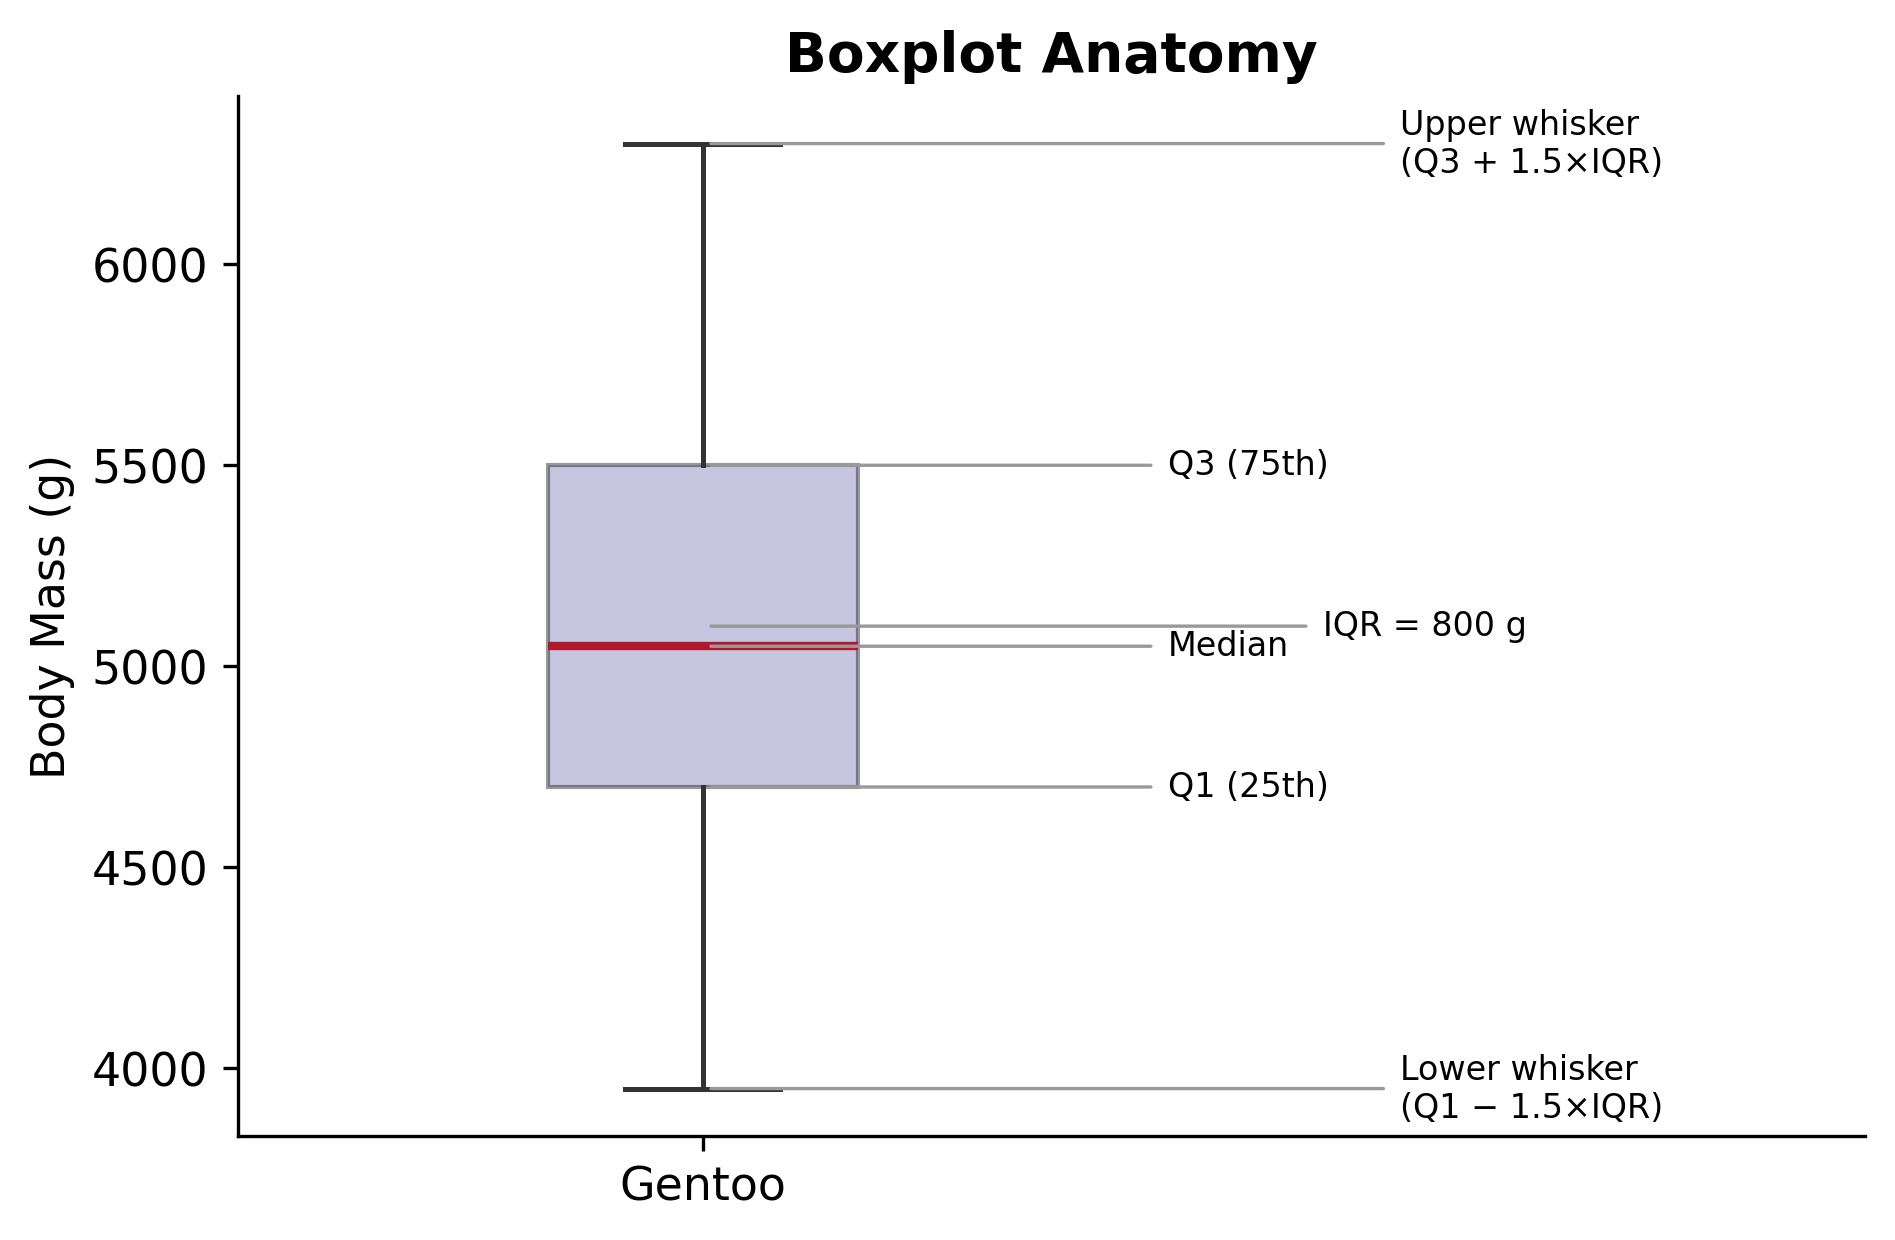
\includegraphics[width=0.62\textwidth]{m2_2_boxplot_anatomy.png}

\vspace{0.2cm}
\begin{exampleblock}{Data Insight}
    \scriptsize Five-number summary: min, Q1, median, Q3, max (with whisker clipping at $1.5 \times \text{IQR}$). Points beyond whiskers are plotted individually as ``outliers.''
\end{exampleblock}
\end{frame}

% ── 34 ──
\begin{frame}{Boxplot: What It Shows and Hides}
\smark{34/300}
\begin{columns}[T]
\begin{column}{0.50\textwidth}
    \textbf{Shows:}
    \begin{itemize}
        \item Median (robust center)
        \item IQR (middle 50\%)
        \item Whisker extent (data range)
        \item Individual outliers
        \item Asymmetry (median off-center)
    \end{itemize}
\end{column}
\begin{column}{0.47\textwidth}
    \textbf{Hides:}
    \begin{itemize}
        \item \textbf{Bimodality} (two peaks look like one wide box)
        \item \textbf{Sample size} ($n=8$ looks like $n=800$)
        \item \textbf{Distribution shape} (uniform, skewed, and normal can produce similar boxes)
        \item \textbf{Gaps and clusters}
    \end{itemize}
\vspace{0.1cm}
\begin{alertblock}{Pro-Tip}
    \scriptsize \textbf{Never publish a standalone boxplot.} Always pair it with raw data (strip) or a density estimate (violin).
\end{alertblock}
\end{column}
\end{columns}
\end{frame}

% ── 35 ──
\begin{frame}[fragile]{Boxplot --- \Rlang}\smark{35/300}
\begin{columns}[T]
\begin{column}{0.55\textwidth}
\begin{lstlisting}[style=Rstyle]
ggplot(penguins,
  aes(species, body_mass_g,
      fill = species)) +
  geom_boxplot(alpha = 0.5,
    outlier.shape = 19,
    outlier.alpha = 0.5) +
  scale_fill_manual(
    values=c("#1B9E77","#D95F02",
             "#7570B3")) +
  theme_minimal() +
  theme(legend.position = "none")
\end{lstlisting}
\end{column}
\begin{column}{0.42\textwidth}
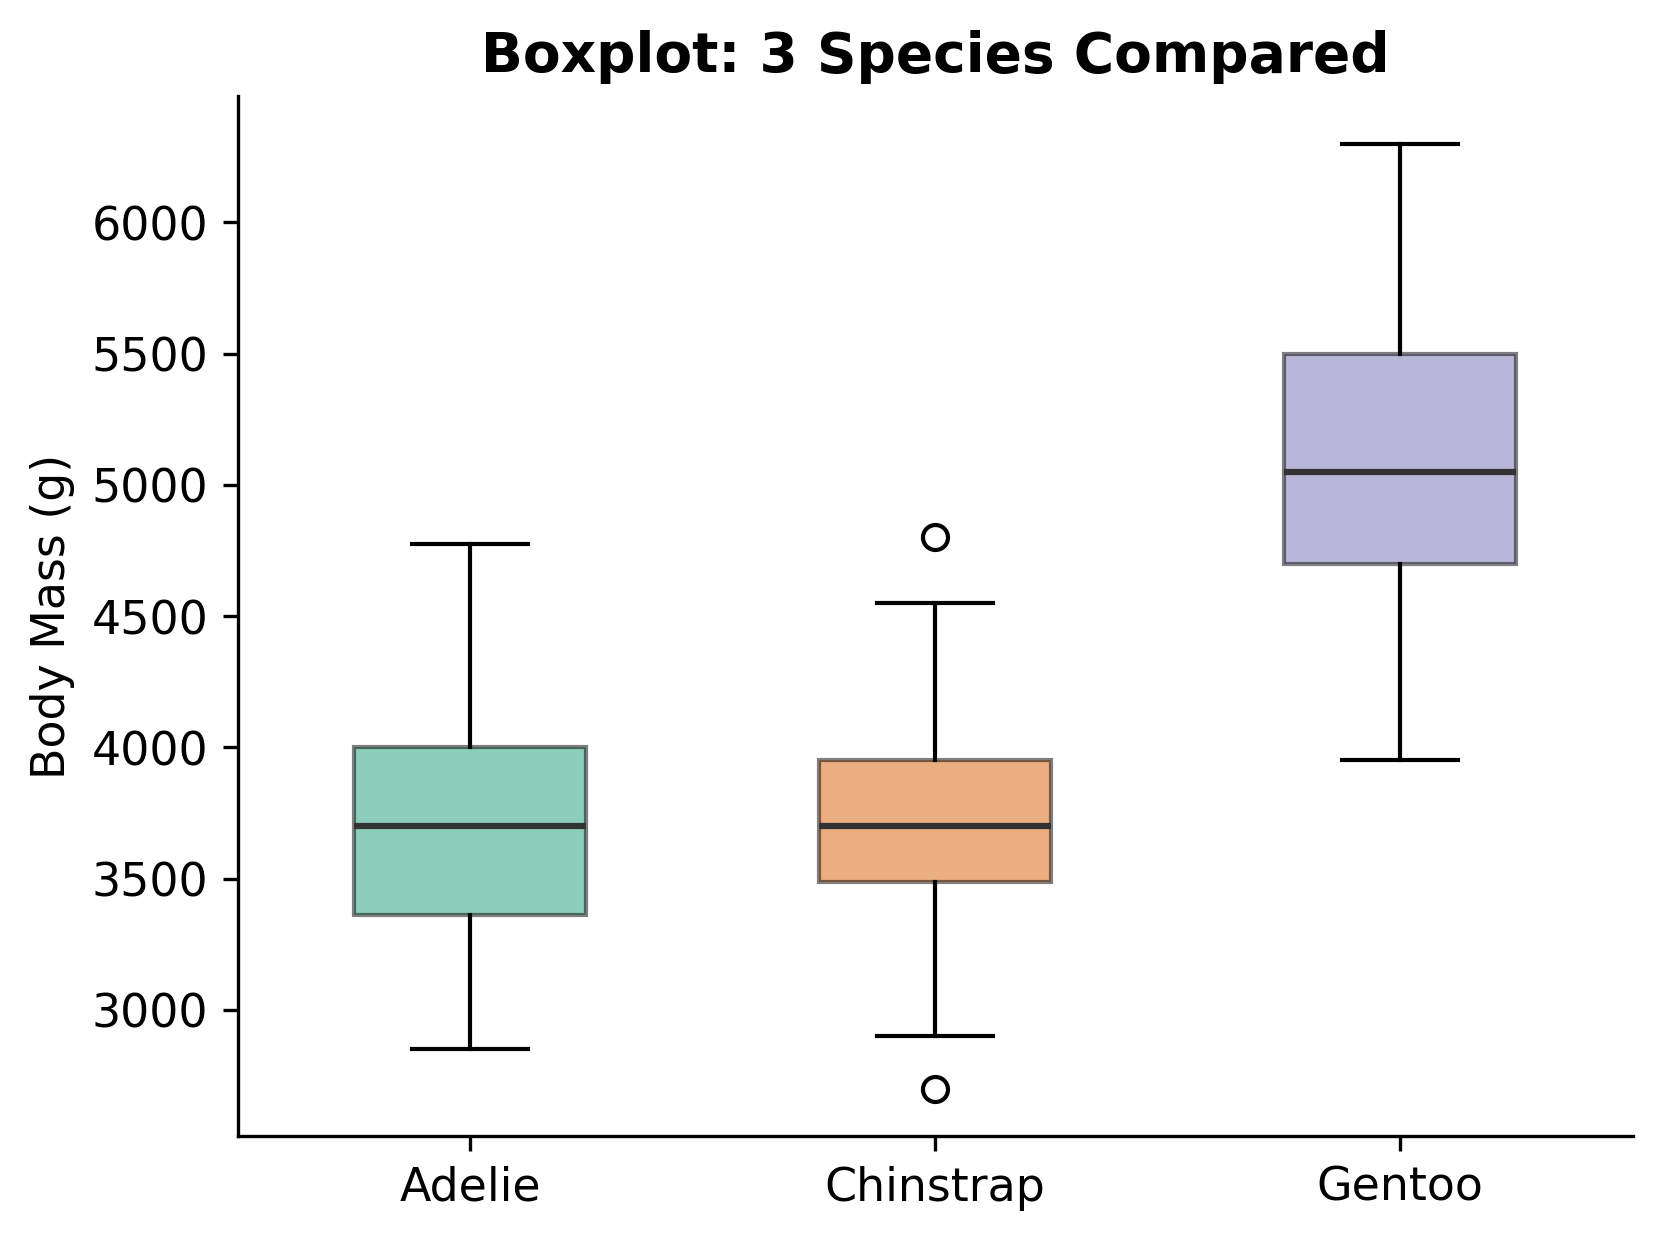
\includegraphics[width=\textwidth]{m2_2_boxplot_compare.png}
\begin{alertblock}{Pro-Tip}
    \scriptsize \texttt{notch=TRUE} adds a confidence interval notch around the median. Non-overlapping notches $\approx$ significantly different medians.
\end{alertblock}
\end{column}
\end{columns}
\end{frame}

% ── 36 ──
\begin{frame}[fragile]{Boxplot --- \Python}\smark{36/300}
\begin{columns}[T]
\begin{column}{0.55\textwidth}
\begin{lstlisting}[style=Pystyle]
# seaborn
sns.boxplot(data=penguins,
    x="species", y="body_mass_g",
    hue="species",
    palette=["#1B9E77","#D95F02",
             "#7570B3"],
    legend=False)

# plotnine
(ggplot(penguins,
   aes("species","body_mass_g",
       fill="species"))
 + geom_boxplot(alpha=0.5)
 + theme(legend_position="none"))

# matplotlib
ax.boxplot([data_per_group],
    patch_artist=True)
\end{lstlisting}
\end{column}
\begin{column}{0.42\textwidth}
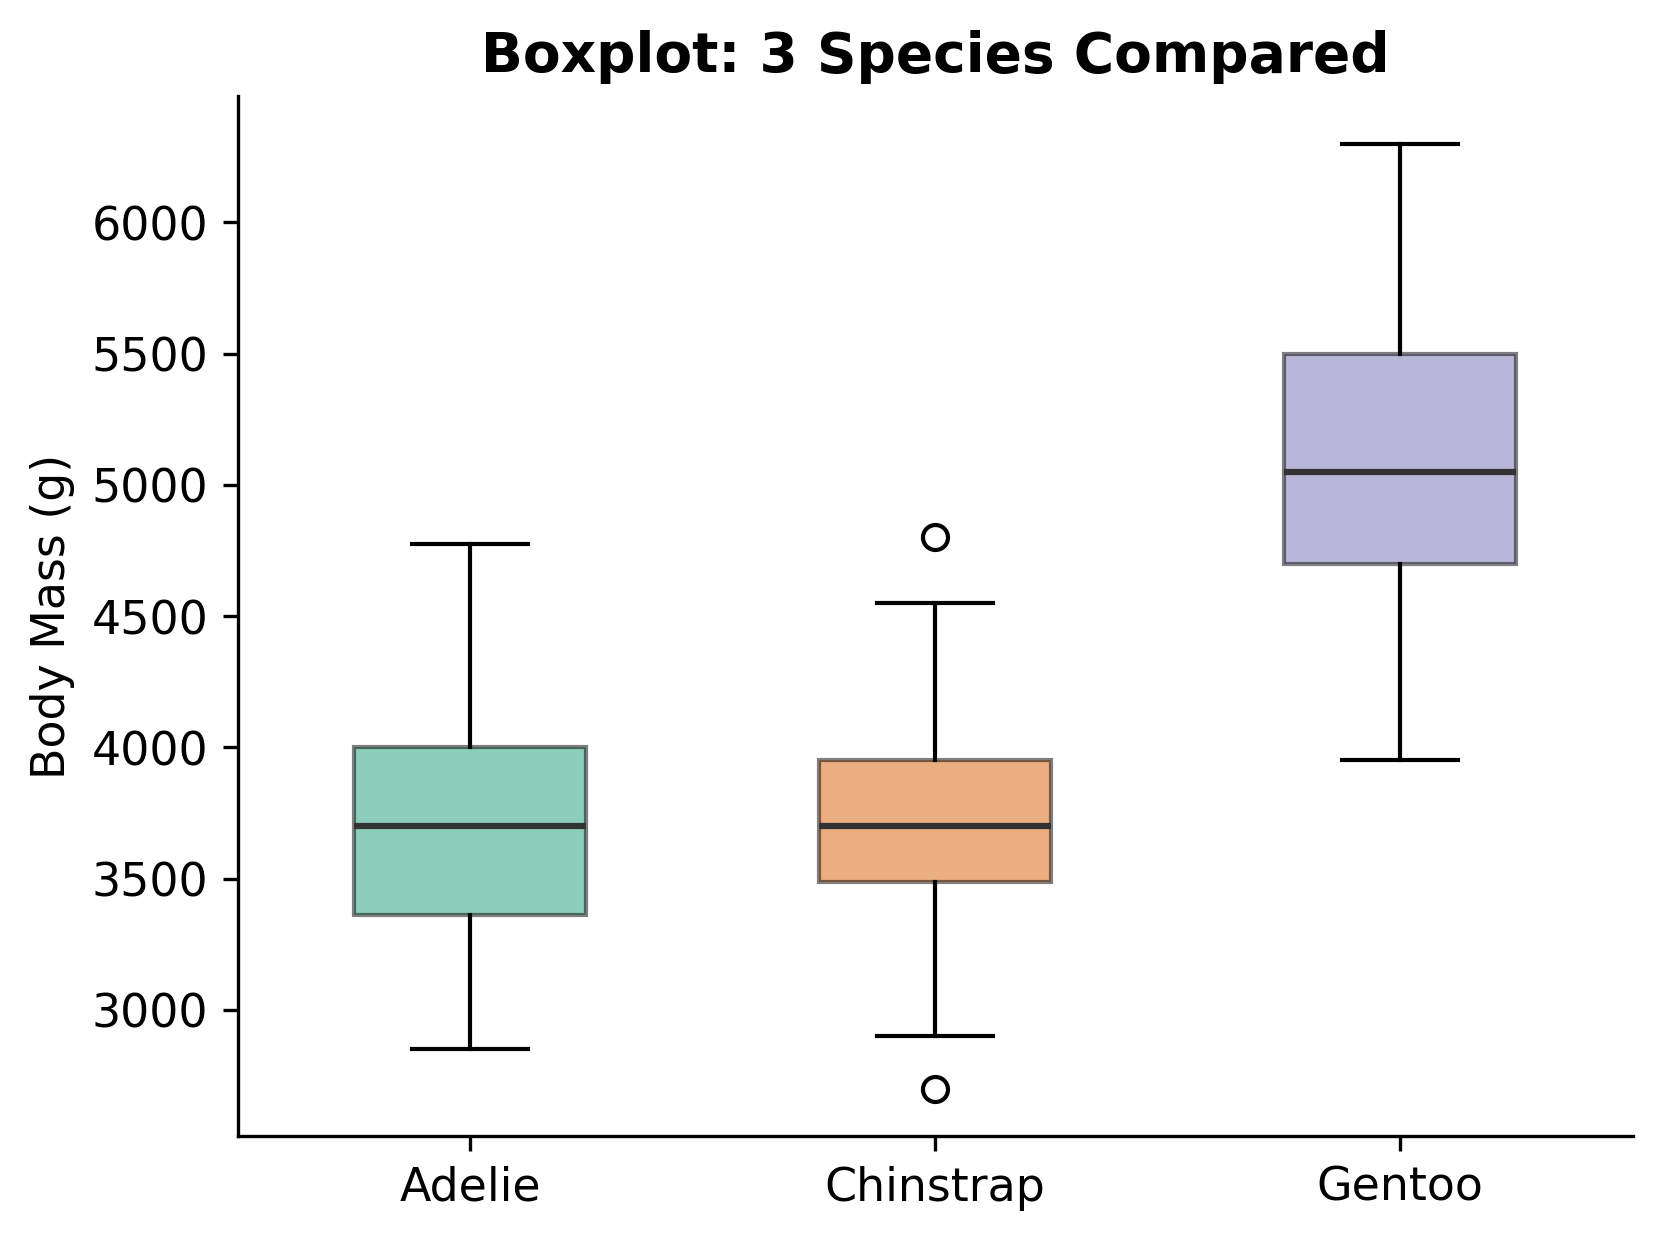
\includegraphics[width=\textwidth]{m2_2_boxplot_compare.png}
\begin{exampleblock}{Data Insight}
    \scriptsize seaborn's \texttt{boxplot()} auto-positions groups. matplotlib's requires manual list input and \texttt{patch\_artist=True} for filled boxes.
\end{exampleblock}
\end{column}
\end{columns}
\end{frame}

% ── 37 ──
\begin{frame}{The Bimodality Trap}
\smark{37/300}
\centering
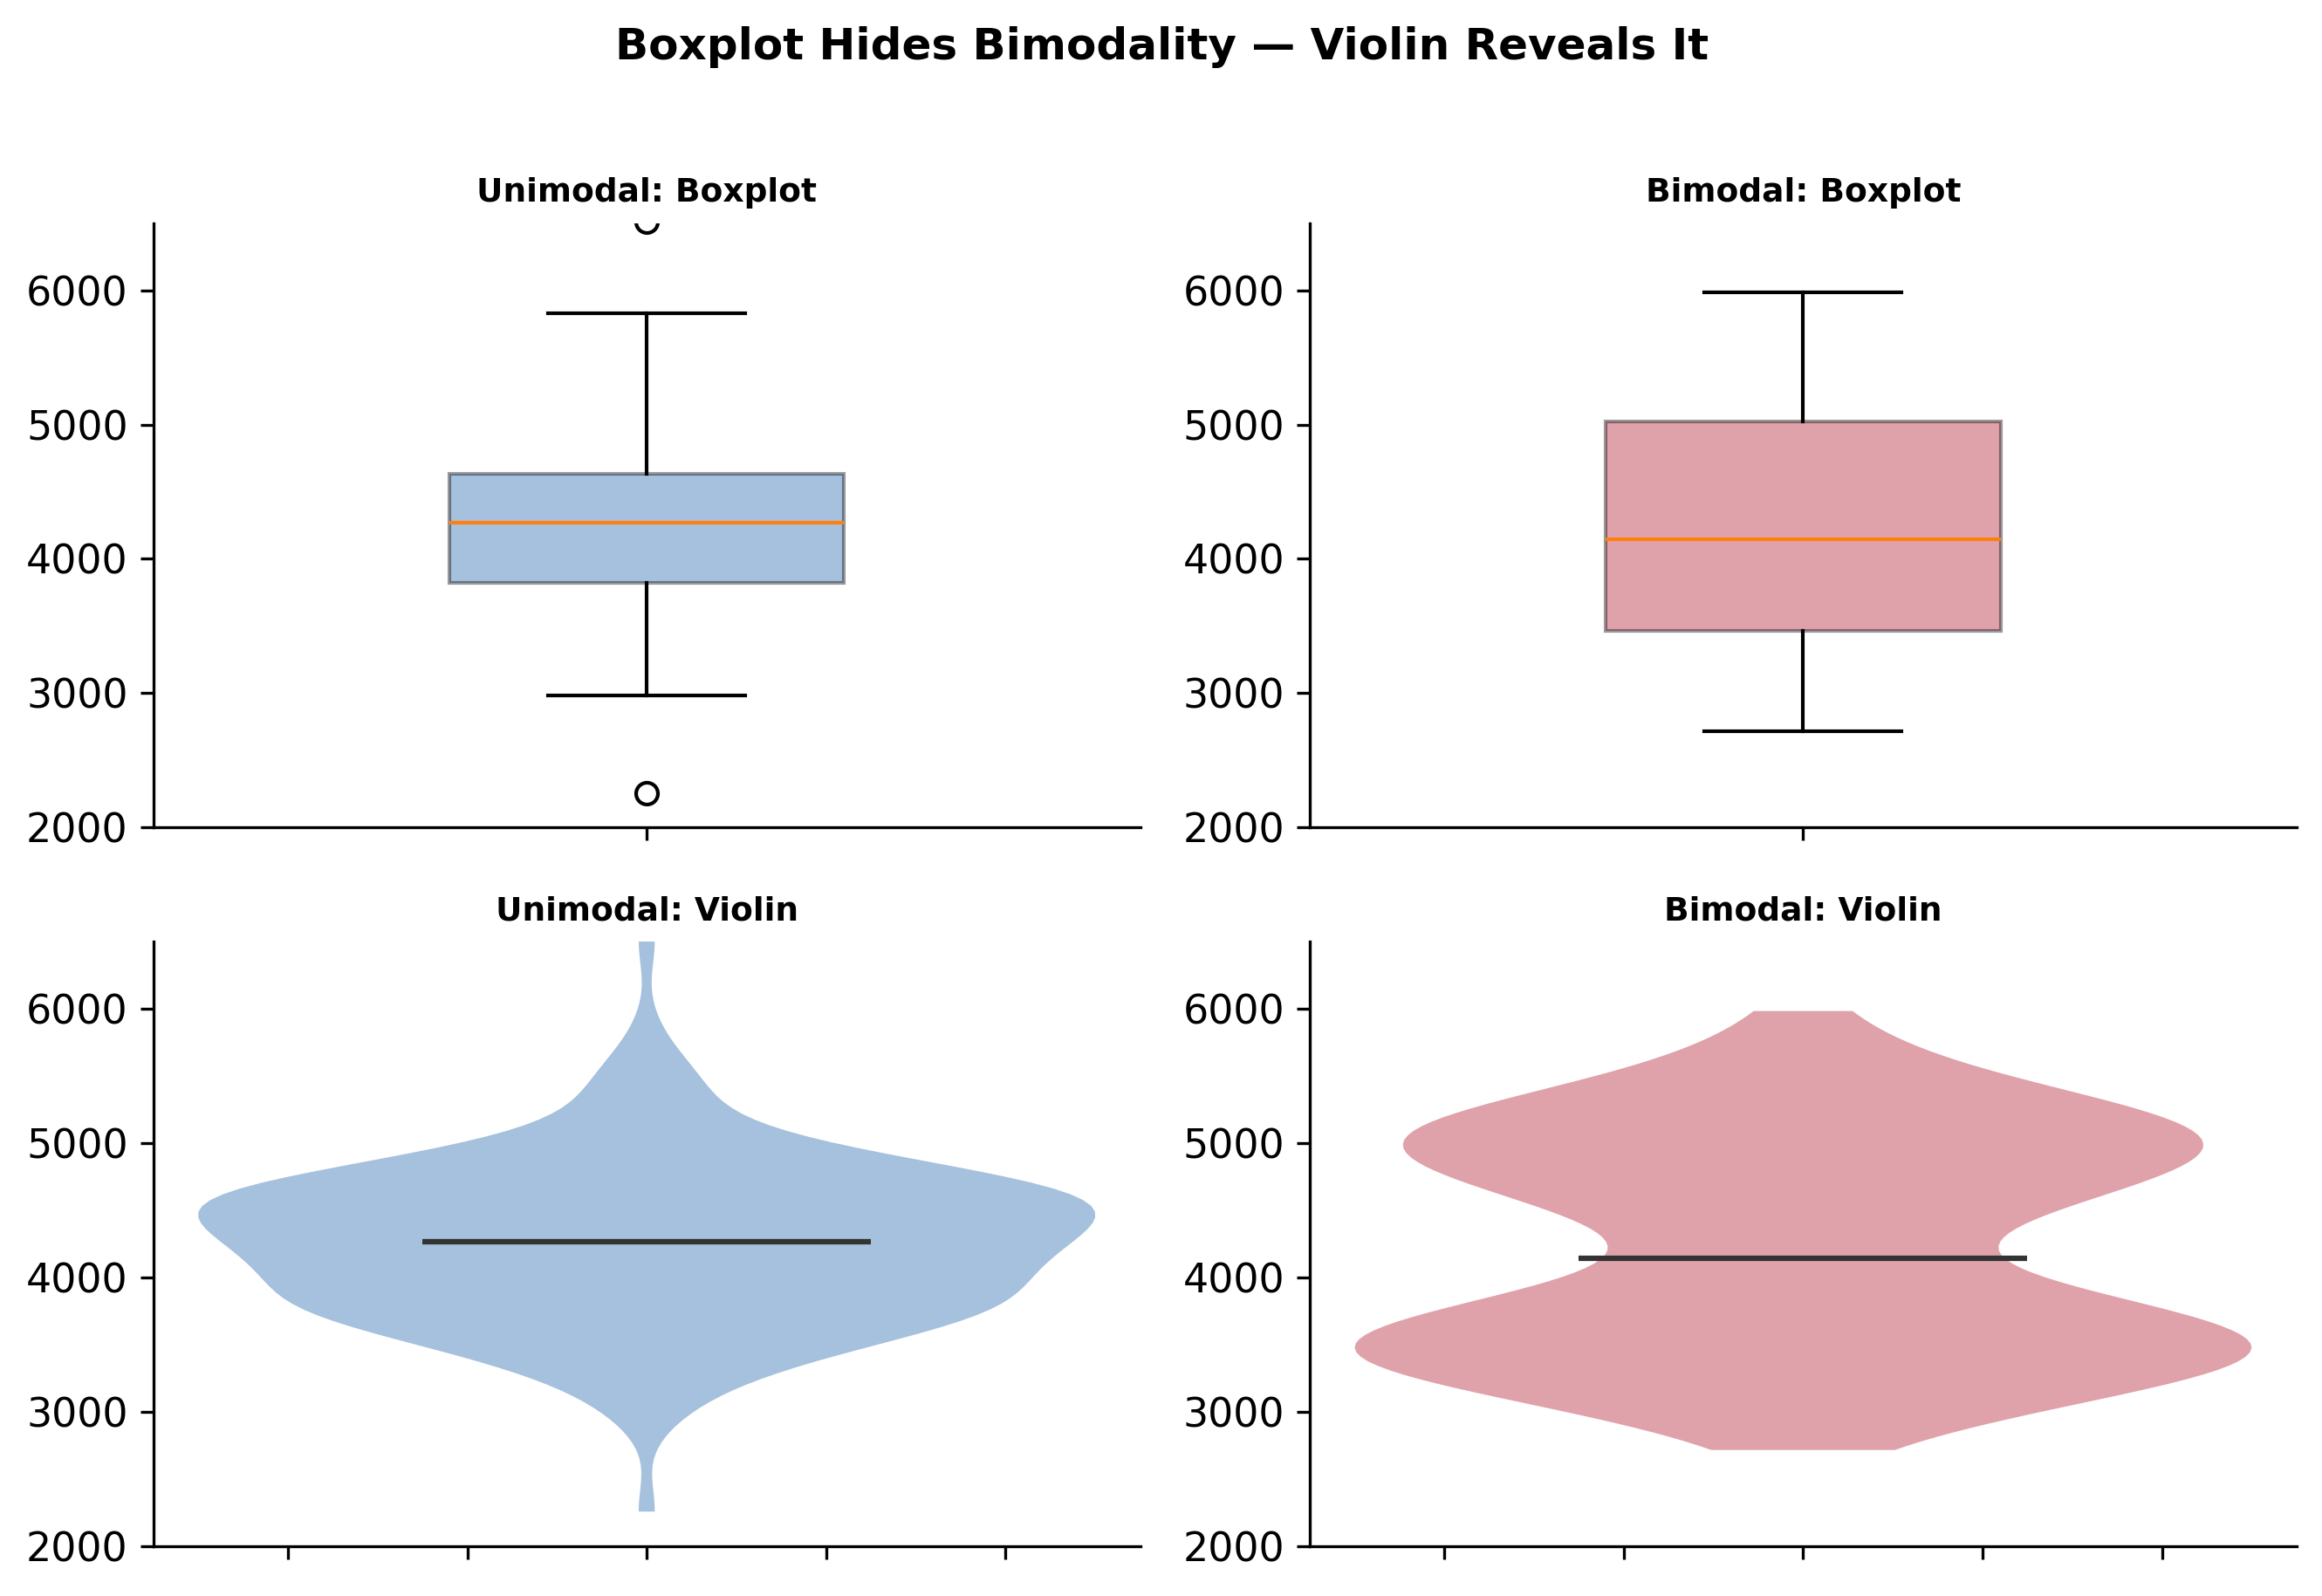
\includegraphics[width=0.85\textwidth]{m2_2_bimodal_trap.png}

\vspace{0.2cm}
\begin{exampleblock}{Data Insight}
    \scriptsize Top row: the boxplots for unimodal and bimodal data look nearly identical --- similar median, IQR, and whisker extent. Bottom row: the violin reveals the bimodal split immediately. This is why violins are strictly superior to standalone boxplots.
\end{exampleblock}
\end{frame}

% ── 38 ──
\begin{frame}{The Violin Plot}
\smark{38/300}
\begin{columns}[T]
\begin{column}{0.50\textwidth}
\begin{itemize}
    \item A \textbf{mirrored KDE} rotated 90\textdegree
    \item Width at each $y$ = local density
    \item Shows distribution \textbf{shape}: skew, bimodality, gaps
    \item No information hiding --- the full density is visible
\end{itemize}
\end{column}
\begin{column}{0.47\textwidth}
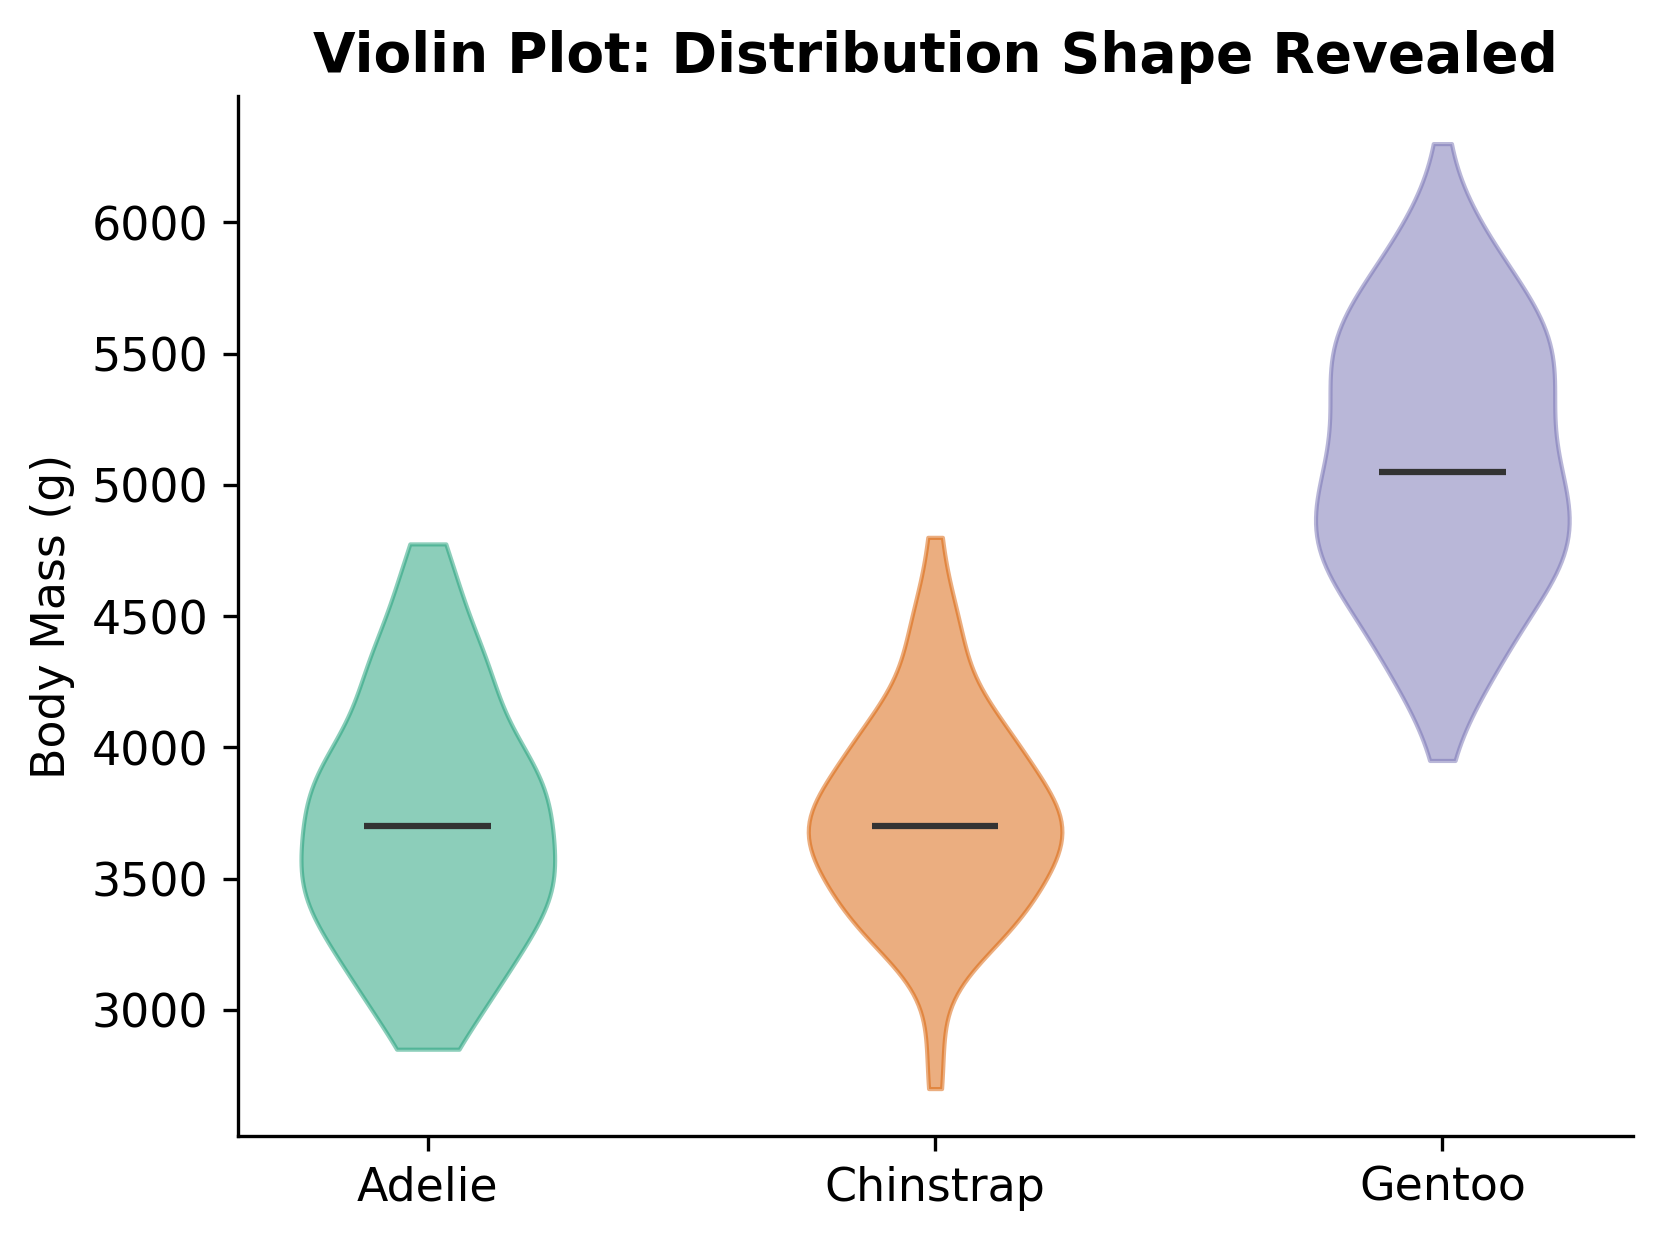
\includegraphics[width=\textwidth]{m2_2_violin.png}
\begin{alertblock}{Pro-Tip}
    \scriptsize Violins can show phantom density in the tails (KDE smoothing beyond data range). Use \texttt{cut=0} in R or \texttt{cut=0} in seaborn to clip the density at observed extremes.
\end{alertblock}
\end{column}
\end{columns}
\end{frame}

% ── 39 ──
\begin{frame}[fragile]{Violin --- \Rlang}\smark{39/300}
\begin{columns}[T]
\begin{column}{0.55\textwidth}
\begin{lstlisting}[style=Rstyle]
ggplot(penguins,
  aes(species, body_mass_g,
      fill = species)) +
  geom_violin(alpha = 0.4,
    trim = FALSE) +
  # Add median line
  stat_summary(fun = median,
    geom = "crossbar",
    width = 0.3, color="#333") +
  scale_fill_manual(
    values=c("#1B9E77","#D95F02",
             "#7570B3")) +
  theme_minimal() +
  theme(legend.position = "none")
\end{lstlisting}
\end{column}
\begin{column}{0.42\textwidth}
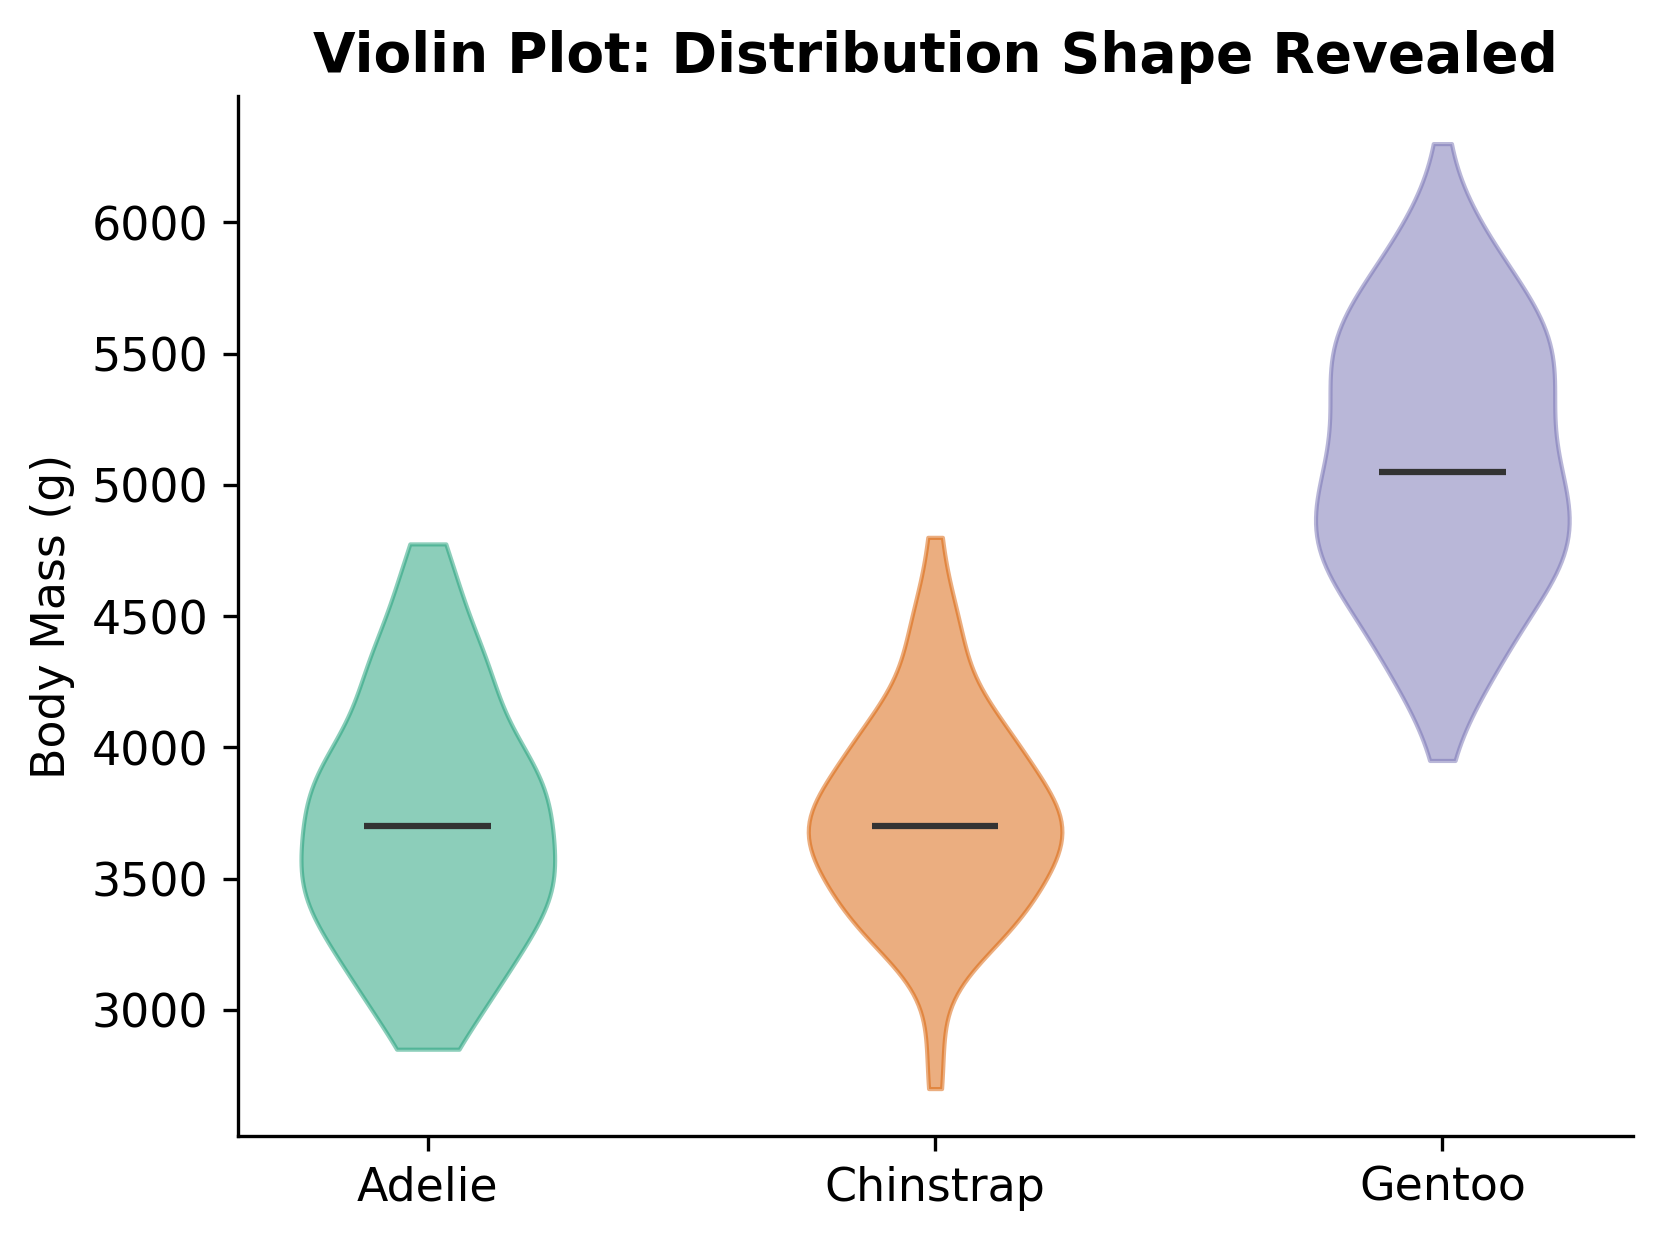
\includegraphics[width=\textwidth]{m2_2_violin.png}
\begin{exampleblock}{Data Insight}
    \scriptsize \texttt{trim=FALSE} extends the KDE to the data range. \texttt{trim=TRUE} (default) clips at the extremes. For honest display, use \texttt{trim=FALSE}.
\end{exampleblock}
\end{column}
\end{columns}
\end{frame}

% ── 40 ──
\begin{frame}[fragile]{Violin --- \Python}\smark{40/300}
\begin{columns}[T]
\begin{column}{0.55\textwidth}
\begin{lstlisting}[style=Pystyle]
# seaborn
sns.violinplot(data=penguins,
    x="species", y="body_mass_g",
    hue="species",
    palette=["#1B9E77","#D95F02",
             "#7570B3"],
    inner="quartile",
    legend=False)

# plotnine
(ggplot(penguins,
   aes("species","body_mass_g",
       fill="species"))
 + geom_violin(alpha=0.4)
 + stat_summary(fun_y=np.median,
     geom="point", size=3))
\end{lstlisting}
\end{column}
\begin{column}{0.42\textwidth}
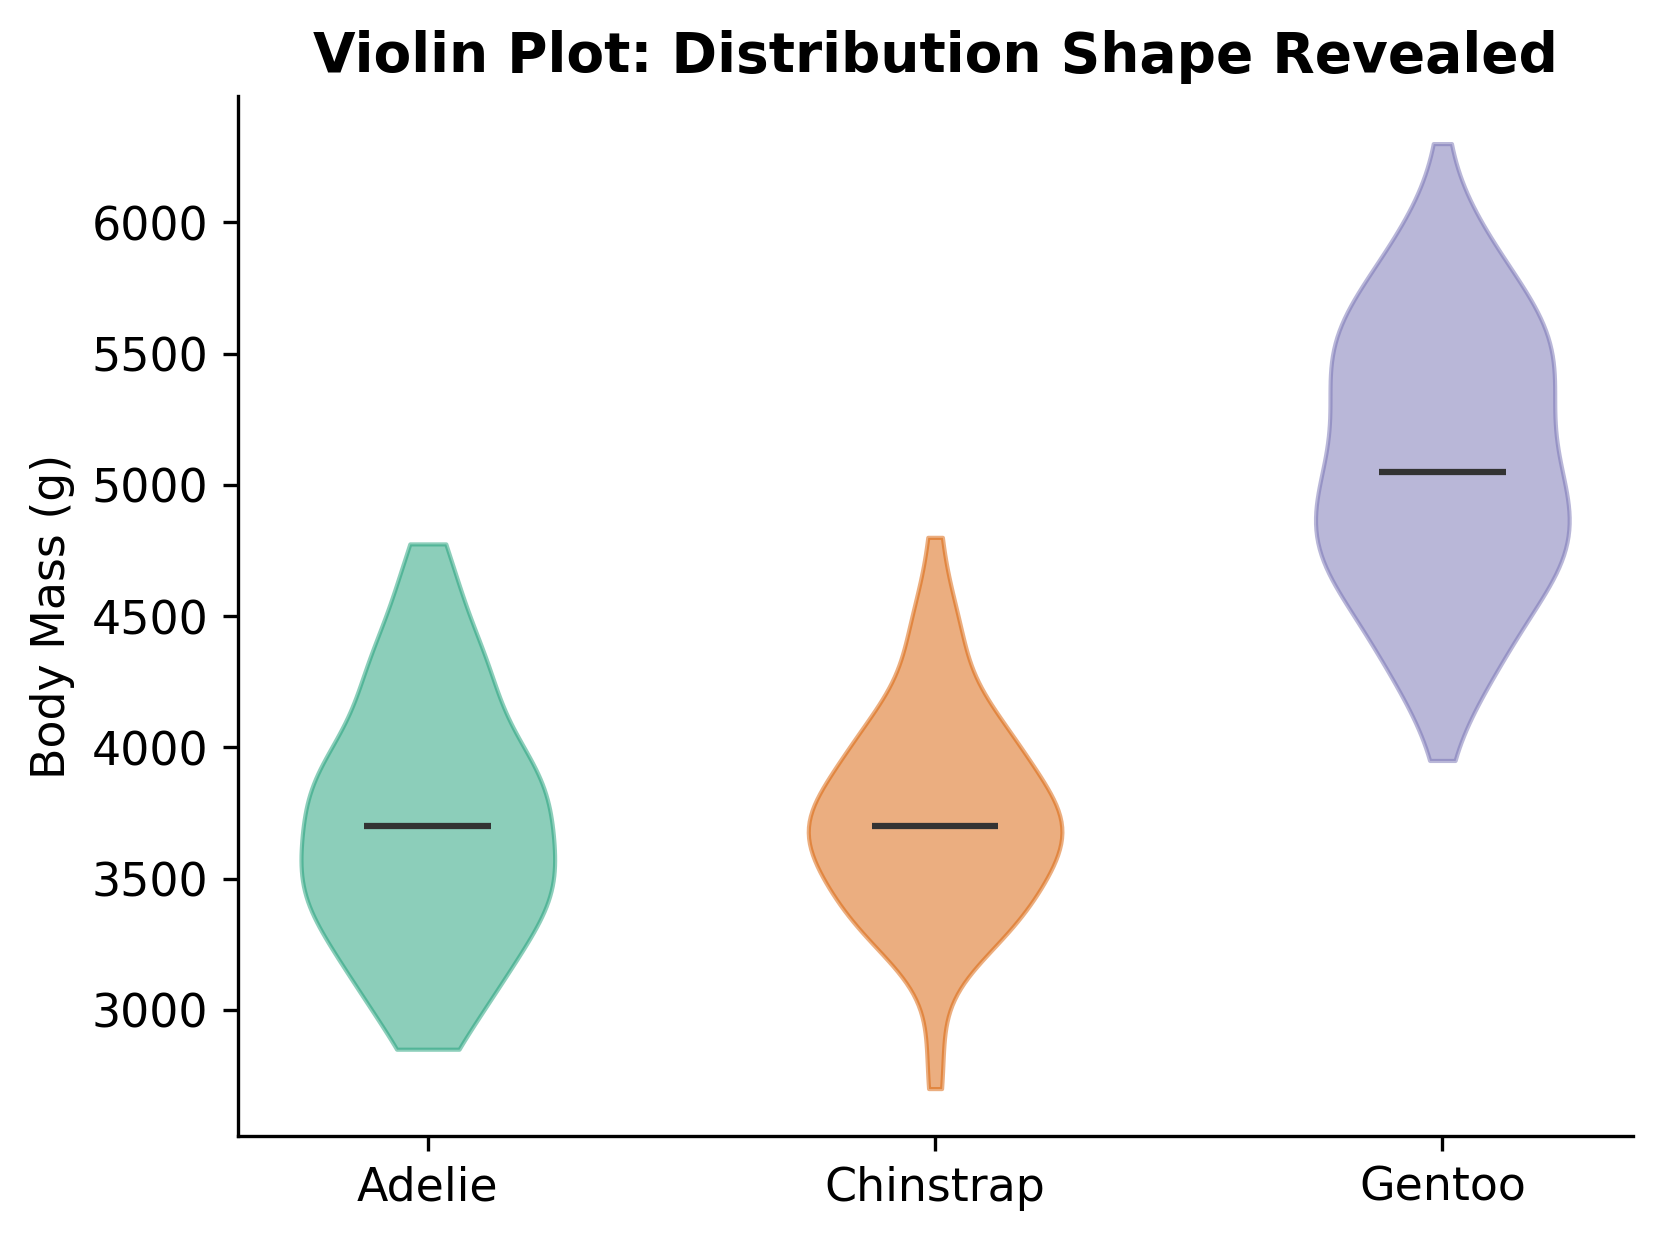
\includegraphics[width=\textwidth]{m2_2_violin.png}
\begin{alertblock}{Pro-Tip}
    \scriptsize seaborn \texttt{inner=} options: \texttt{"quartile"} (dashed lines), \texttt{"box"} (mini boxplot), \texttt{"point"} (raw points), \texttt{"stick"} (rug). \texttt{"quartile"} is the best default.
\end{alertblock}
\end{column}
\end{columns}
\end{frame}

% ── 41 ──
\begin{frame}{Violin + Box + Jitter: The Best of All Worlds}
\smark{41/300}
\centering
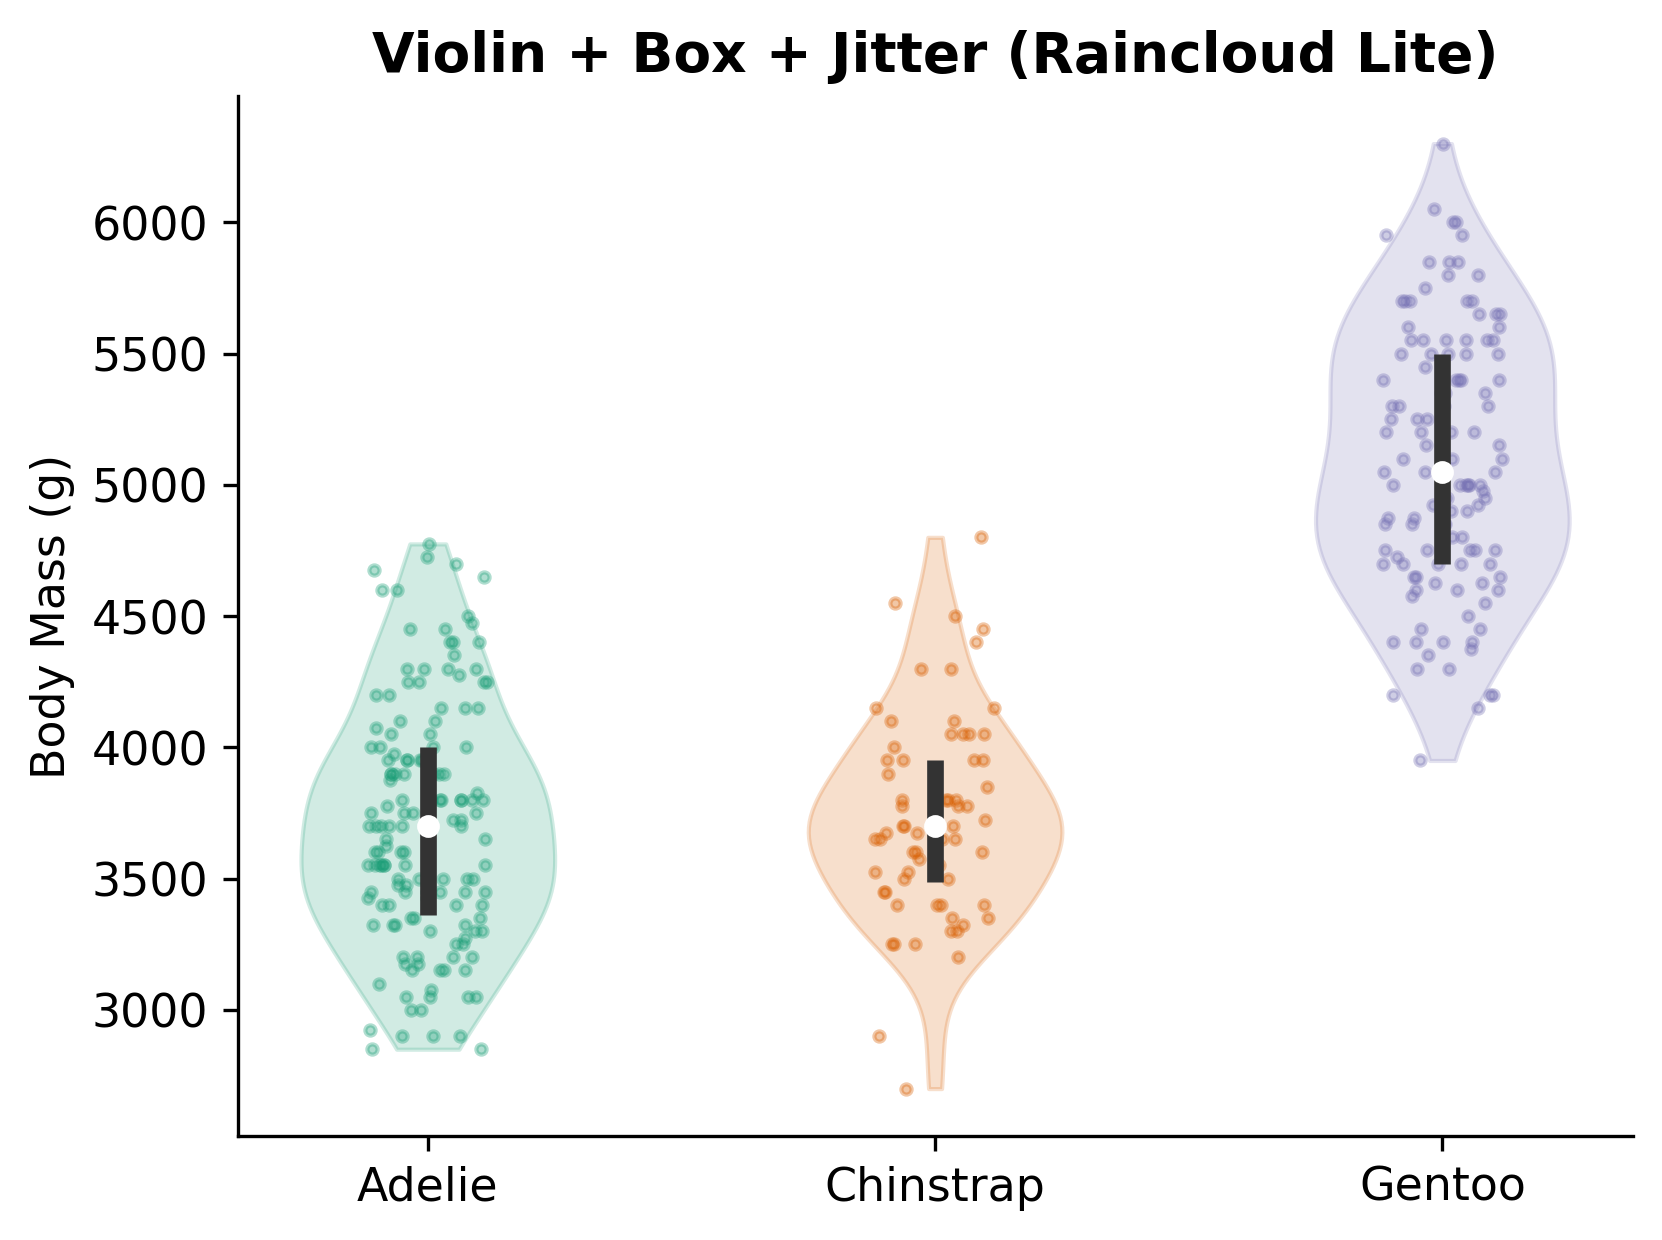
\includegraphics[width=0.65\textwidth]{m2_2_violin_box_jitter.png}

\vspace{0.2cm}
\begin{exampleblock}{Data Insight}
    \scriptsize The violin shows shape, the box shows quartiles, and the jittered points show every observation. Three complementary views layered on one axis --- the maximum-information display for grouped continuous data.
\end{exampleblock}
\end{frame}

% ── 42 ──
\begin{frame}[fragile]{Violin + Box + Jitter --- \Rlang}\smark{42/300}
\begin{columns}[T]
\begin{column}{0.55\textwidth}
\begin{lstlisting}[style=Rstyle]
ggplot(penguins,
  aes(species, body_mass_g,
      fill = species)) +
  # Layer 1: violin
  geom_violin(alpha = 0.2,
    color = NA) +
  # Layer 2: mini boxplot
  geom_boxplot(width = 0.15,
    outlier.shape = NA,
    alpha = 0.6) +
  # Layer 3: jittered points
  geom_jitter(width = 0.1,
    alpha = 0.3, size = 1,
    color = "#333") +
  theme_minimal() +
  theme(legend.position="none")
\end{lstlisting}
\end{column}
\begin{column}{0.42\textwidth}
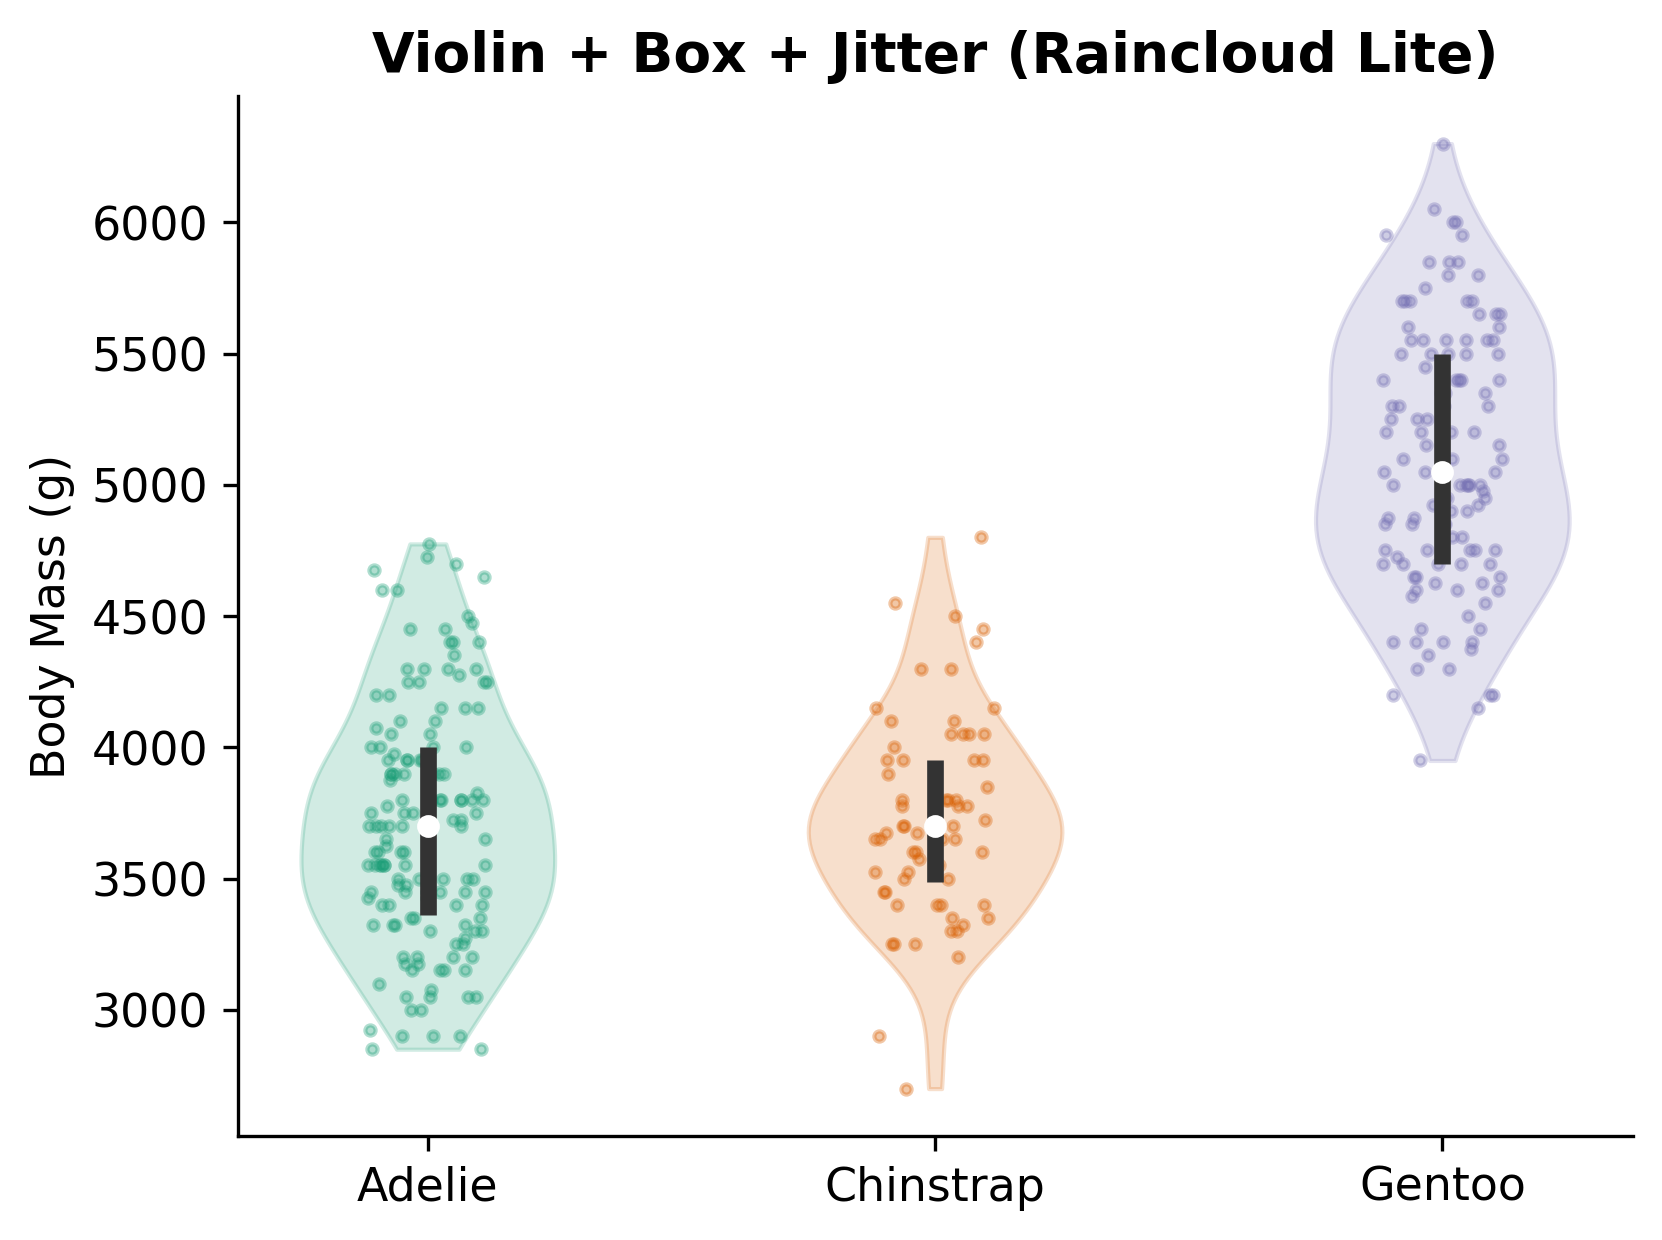
\includegraphics[width=\textwidth]{m2_2_violin_box_jitter.png}
\begin{alertblock}{Pro-Tip}
    \scriptsize Key settings: \texttt{color=NA} on the violin removes the outline. \texttt{width=0.15} on the box keeps it narrow inside the violin. \texttt{outlier.shape=NA} avoids duplicate points.
\end{alertblock}
\end{column}
\end{columns}
\end{frame}

% ── 43 ──
\begin{frame}[fragile]{Violin + Box + Jitter --- \Python}\smark{43/300}
\begin{columns}[T]
\begin{column}{0.55\textwidth}
\begin{lstlisting}[style=Pystyle]
fig, ax = plt.subplots()

# Layer 1: violin
sns.violinplot(data=penguins,
    x="species", y="body_mass_g",
    inner=None, palette=D,
    alpha=0.2, ax=ax)

# Layer 2: mini boxplot
sns.boxplot(data=penguins,
    x="species", y="body_mass_g",
    width=0.15, showfliers=False,
    boxprops=dict(alpha=0.6),
    ax=ax)

# Layer 3: strip
sns.stripplot(data=penguins,
    x="species", y="body_mass_g",
    jitter=0.1, alpha=0.3, s=2,
    color="#333", ax=ax)
\end{lstlisting}
\end{column}
\begin{column}{0.42\textwidth}
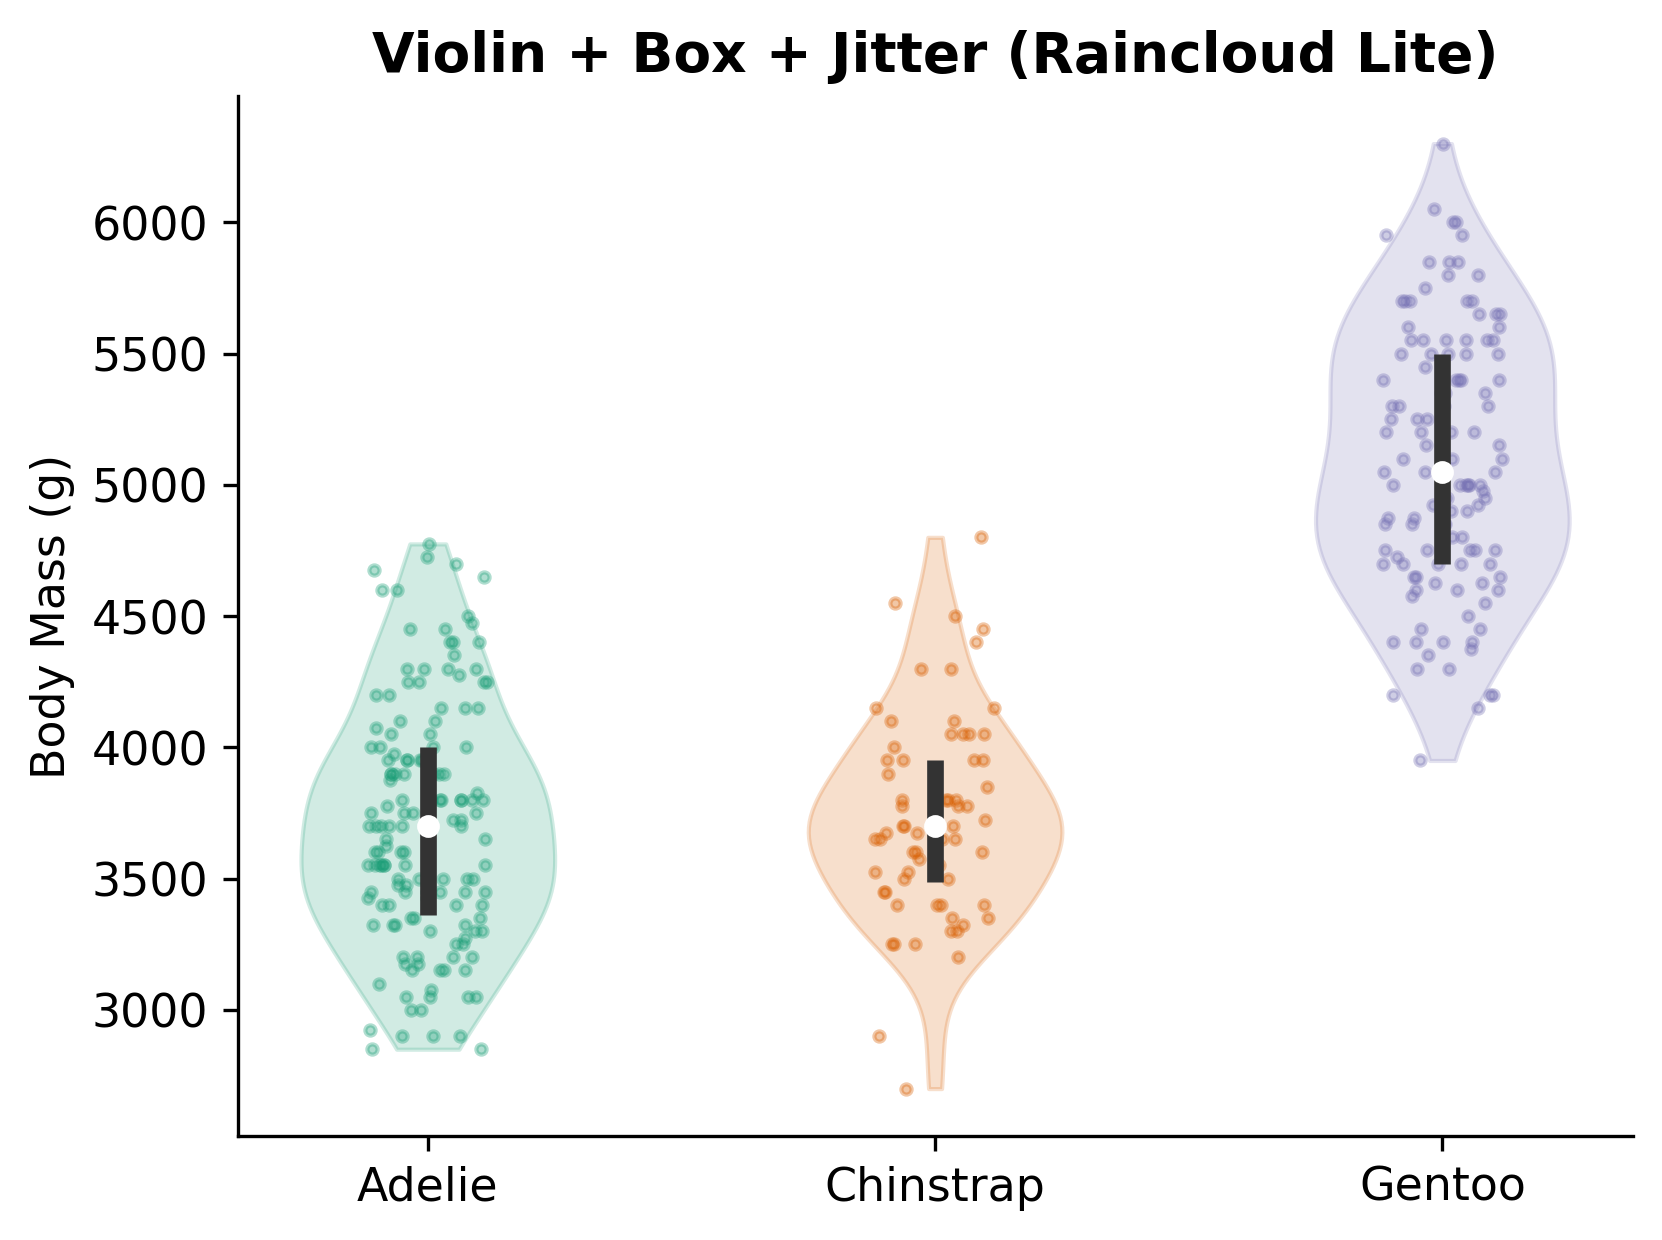
\includegraphics[width=\textwidth]{m2_2_violin_box_jitter.png}
\begin{exampleblock}{Data Insight}
    \scriptsize In seaborn, \texttt{inner=None} removes the default quartile lines from the violin, letting the overlaid boxplot handle that role without visual clutter.
\end{exampleblock}
\end{column}
\end{columns}
\end{frame}

% ── 44 ──
\begin{frame}{Raincloud Plots}
\smark{44/300}
\centering
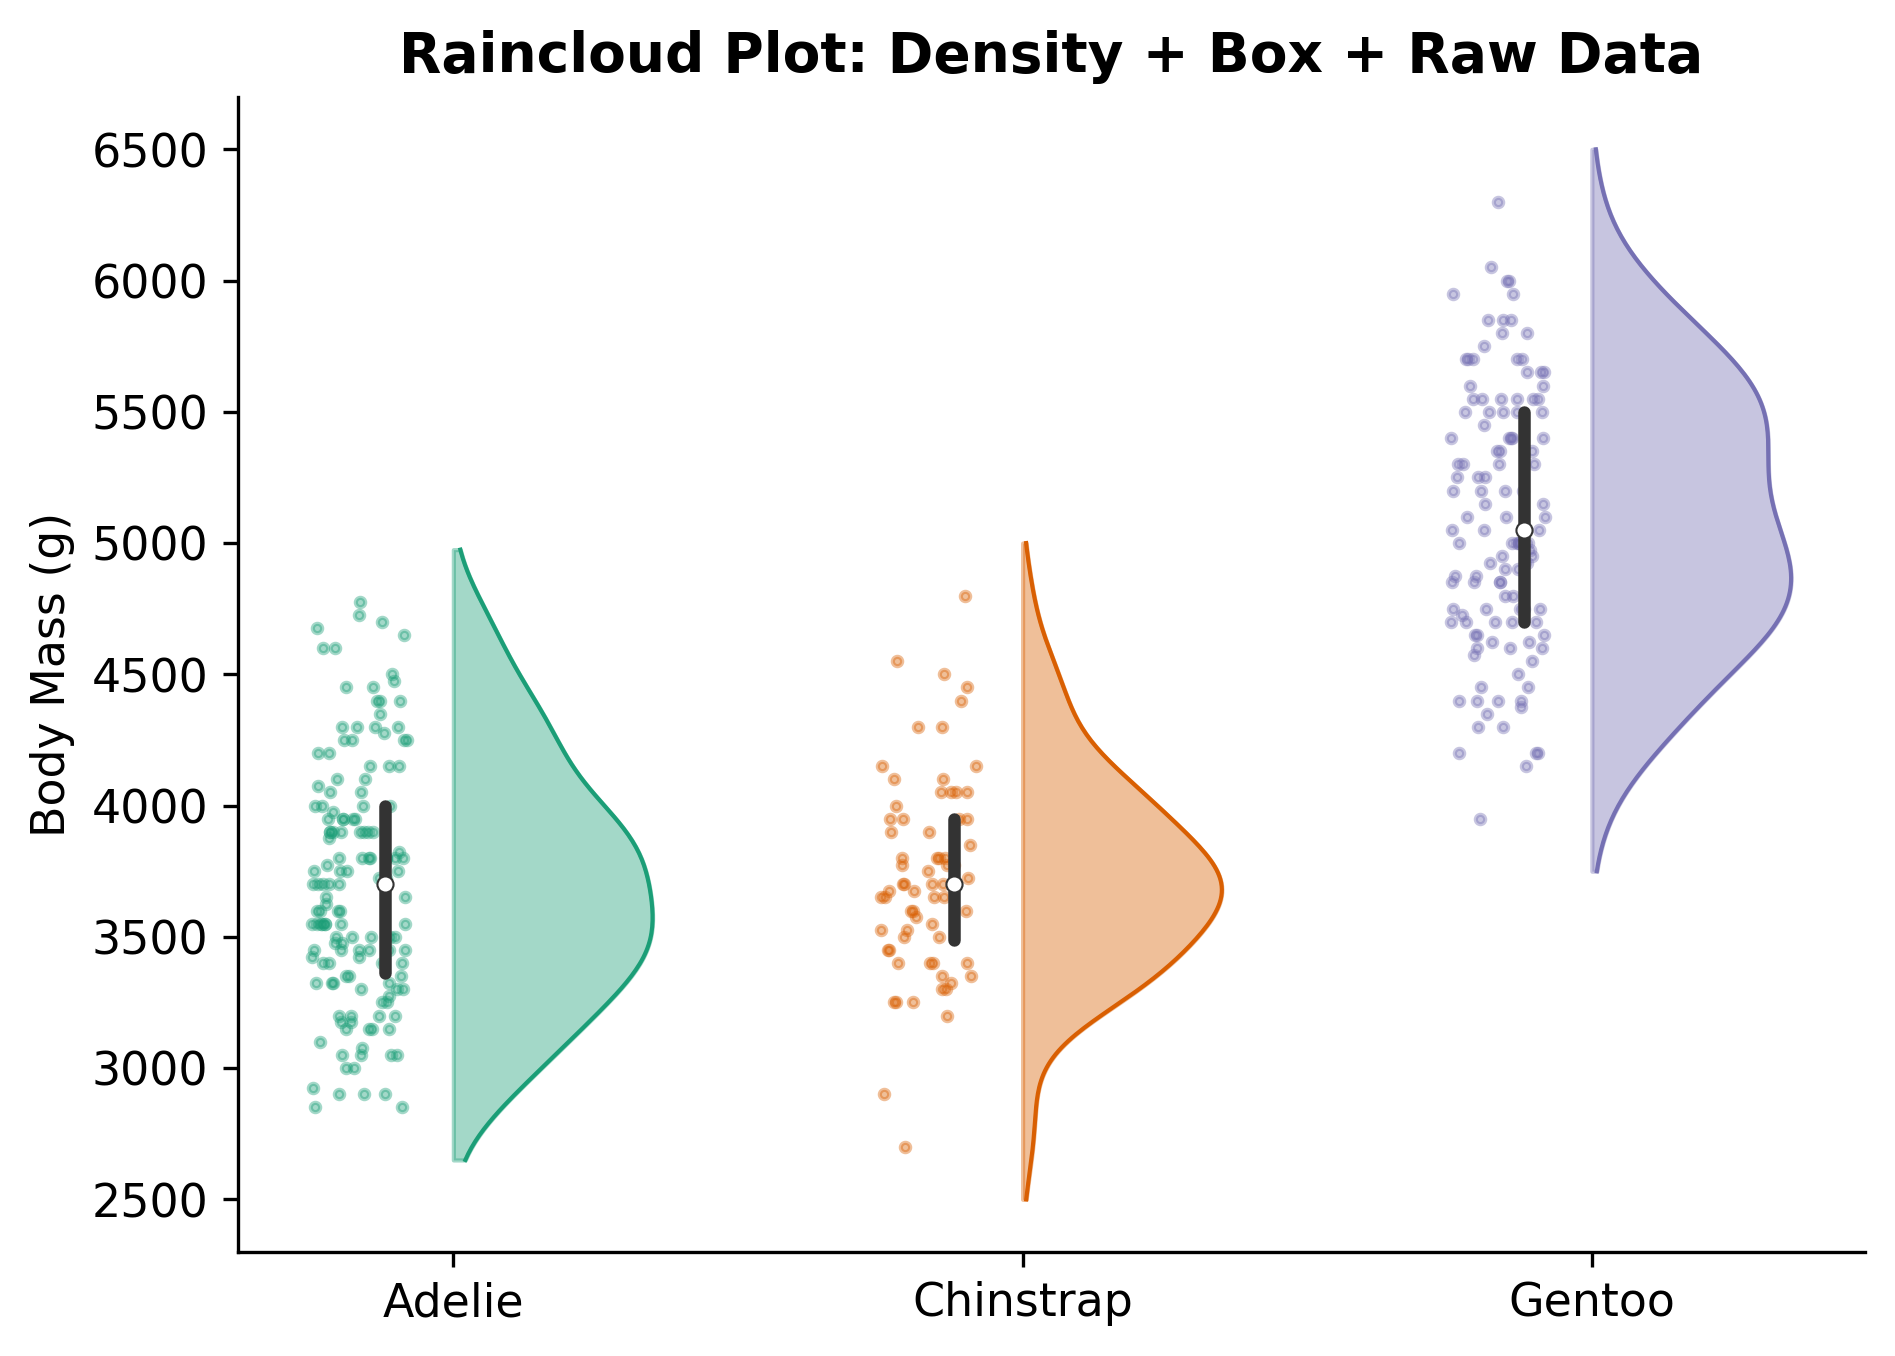
\includegraphics[width=0.65\textwidth]{m2_2_raincloud.png}

\vspace{0.2cm}
\begin{columns}[T]
\begin{column}{0.48\textwidth}
\begin{itemize}
    \item \textbf{Half-violin} (cloud) above
    \item \textbf{Mini boxplot} (lightning) in the middle
    \item \textbf{Jittered points} (rain) below
    \item Allen et al.\ (2019): ``Raincloud plots: a multi-platform tool for robust data visualization''
\end{itemize}
\end{column}
\begin{column}{0.48\textwidth}
\begin{exampleblock}{Data Insight}
    \scriptsize The asymmetric layout avoids the mirror-image redundancy of standard violins. Every pixel carries unique information: density, summary, or raw observation.
\end{exampleblock}
\end{column}
\end{columns}
\end{frame}

% ── 45 ──
\begin{frame}[fragile]{Raincloud --- \Rlang}\smark{45/300}
\begin{columns}[T]
\begin{column}{0.55\textwidth}
\begin{lstlisting}[style=Rstyle]
library(ggdist)  # OR ggrain

ggplot(penguins,
  aes(species, body_mass_g,
      fill = species)) +
  # Half-violin (cloud)
  stat_halfeye(
    adjust = 0.5, width = 0.6,
    justification = -0.2,
    .width = 0, point_colour=NA)+
  # Boxplot (lightning)
  geom_boxplot(width = 0.12,
    outlier.shape = NA,
    alpha = 0.5) +
  # Jitter (rain)
  geom_jitter(width = 0.05,
    alpha = 0.3, size = 1) +
  coord_flip() +
  theme_minimal() +
  theme(legend.position="none")
\end{lstlisting}
\end{column}
\begin{column}{0.42\textwidth}
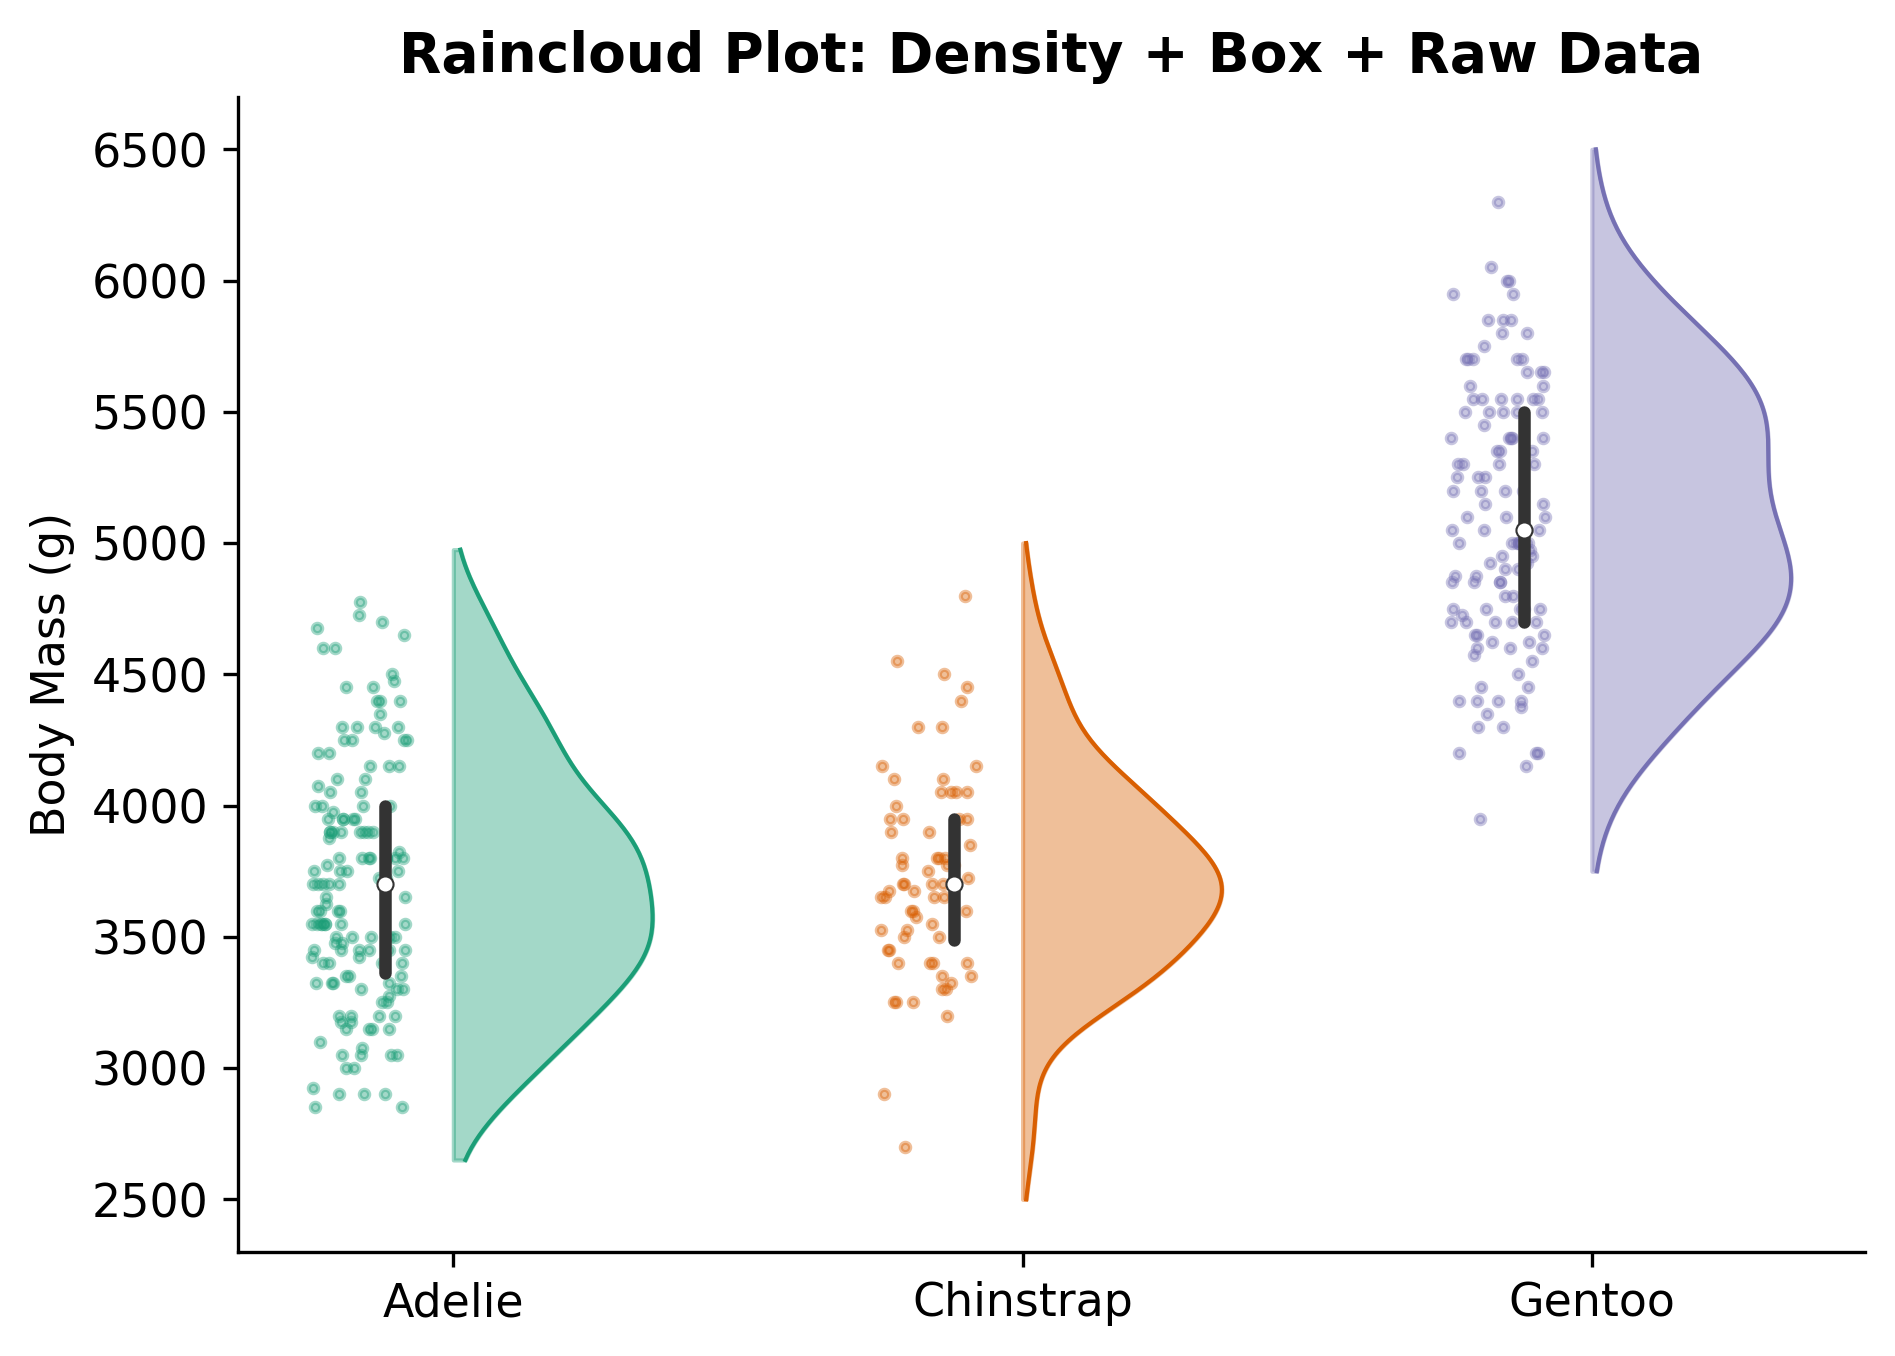
\includegraphics[width=\textwidth]{m2_2_raincloud.png}
\begin{alertblock}{Pro-Tip}
    \scriptsize \texttt{ggdist::stat\_halfeye()} is the cleanest R approach. Alternative: \texttt{ggrain::geom\_rain()} provides a single-layer raincloud. Both CRAN-available.
\end{alertblock}
\end{column}
\end{columns}
\end{frame}

% ── 46 ──
\begin{frame}[fragile]{Raincloud --- \Python}\smark{46/300}
\begin{columns}[T]
\begin{column}{0.55\textwidth}
\begin{lstlisting}[style=Pystyle]
# pip install ptitprince
import ptitprince as pt

fig, ax = plt.subplots()
pt.RainCloud(data=penguins,
    x="species", y="body_mass_g",
    palette=["#1B9E77","#D95F02",
             "#7570B3"],
    orient="v",
    ax=ax, alpha=0.5,
    point_size=3,
    bw=0.2)

# OR manual approach:
# 1. Half-violin (scipy KDE)
# 2. ax.boxplot()
# 3. ax.scatter() with jitter
\end{lstlisting}
\end{column}
\begin{column}{0.42\textwidth}
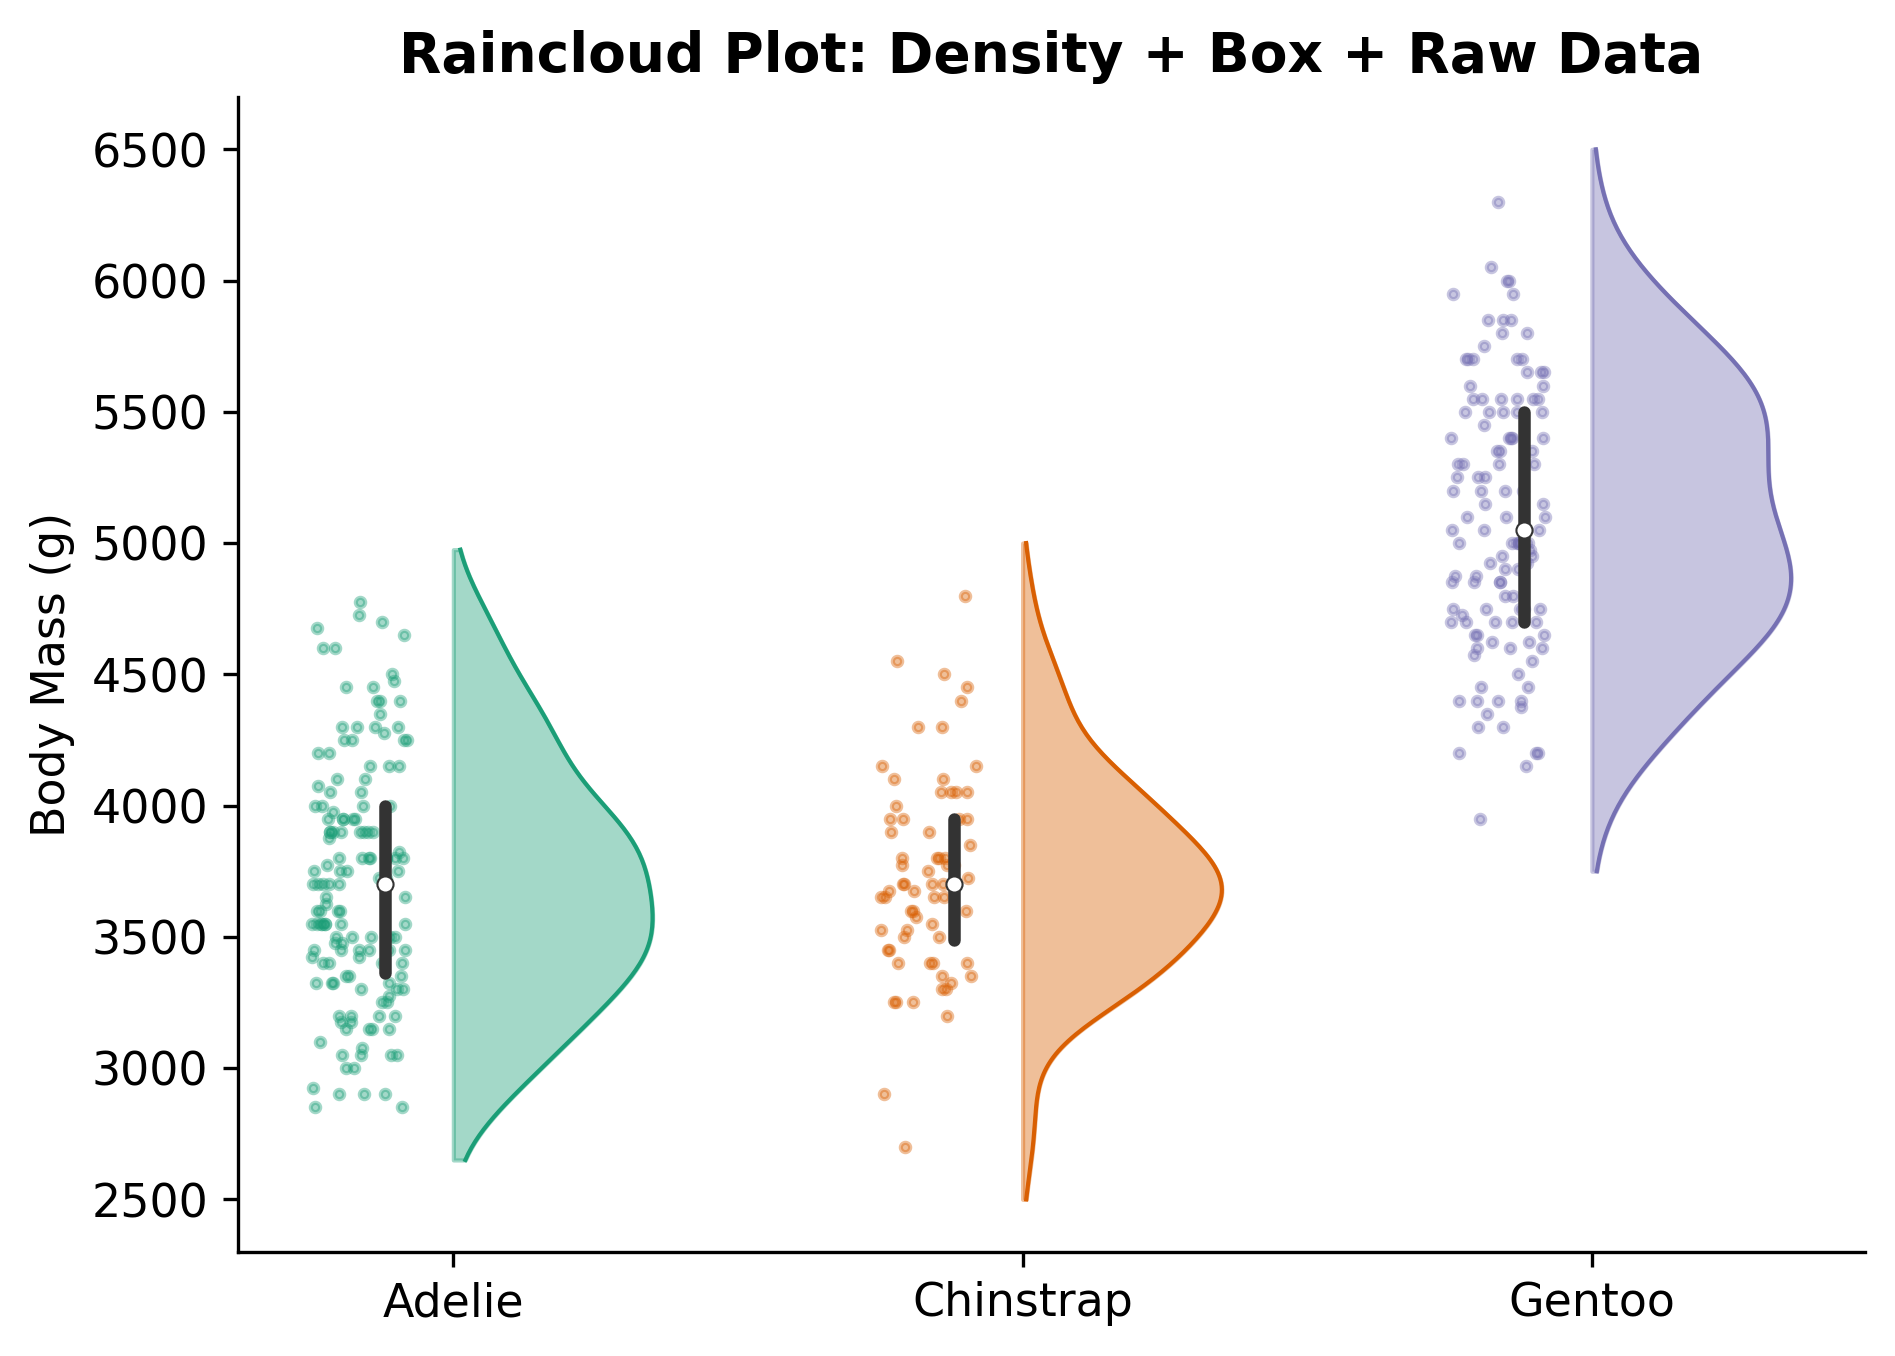
\includegraphics[width=\textwidth]{m2_2_raincloud.png}
\begin{exampleblock}{Data Insight}
    \scriptsize \texttt{ptitprince.RainCloud()} is the Python port of the original R raincloud paper. It handles all three layers in one call.
\end{exampleblock}
\end{column}
\end{columns}
\end{frame}

% ── 47 ──
\begin{frame}{Beeswarm and Sina Plots}
\smark{47/300}
\centering
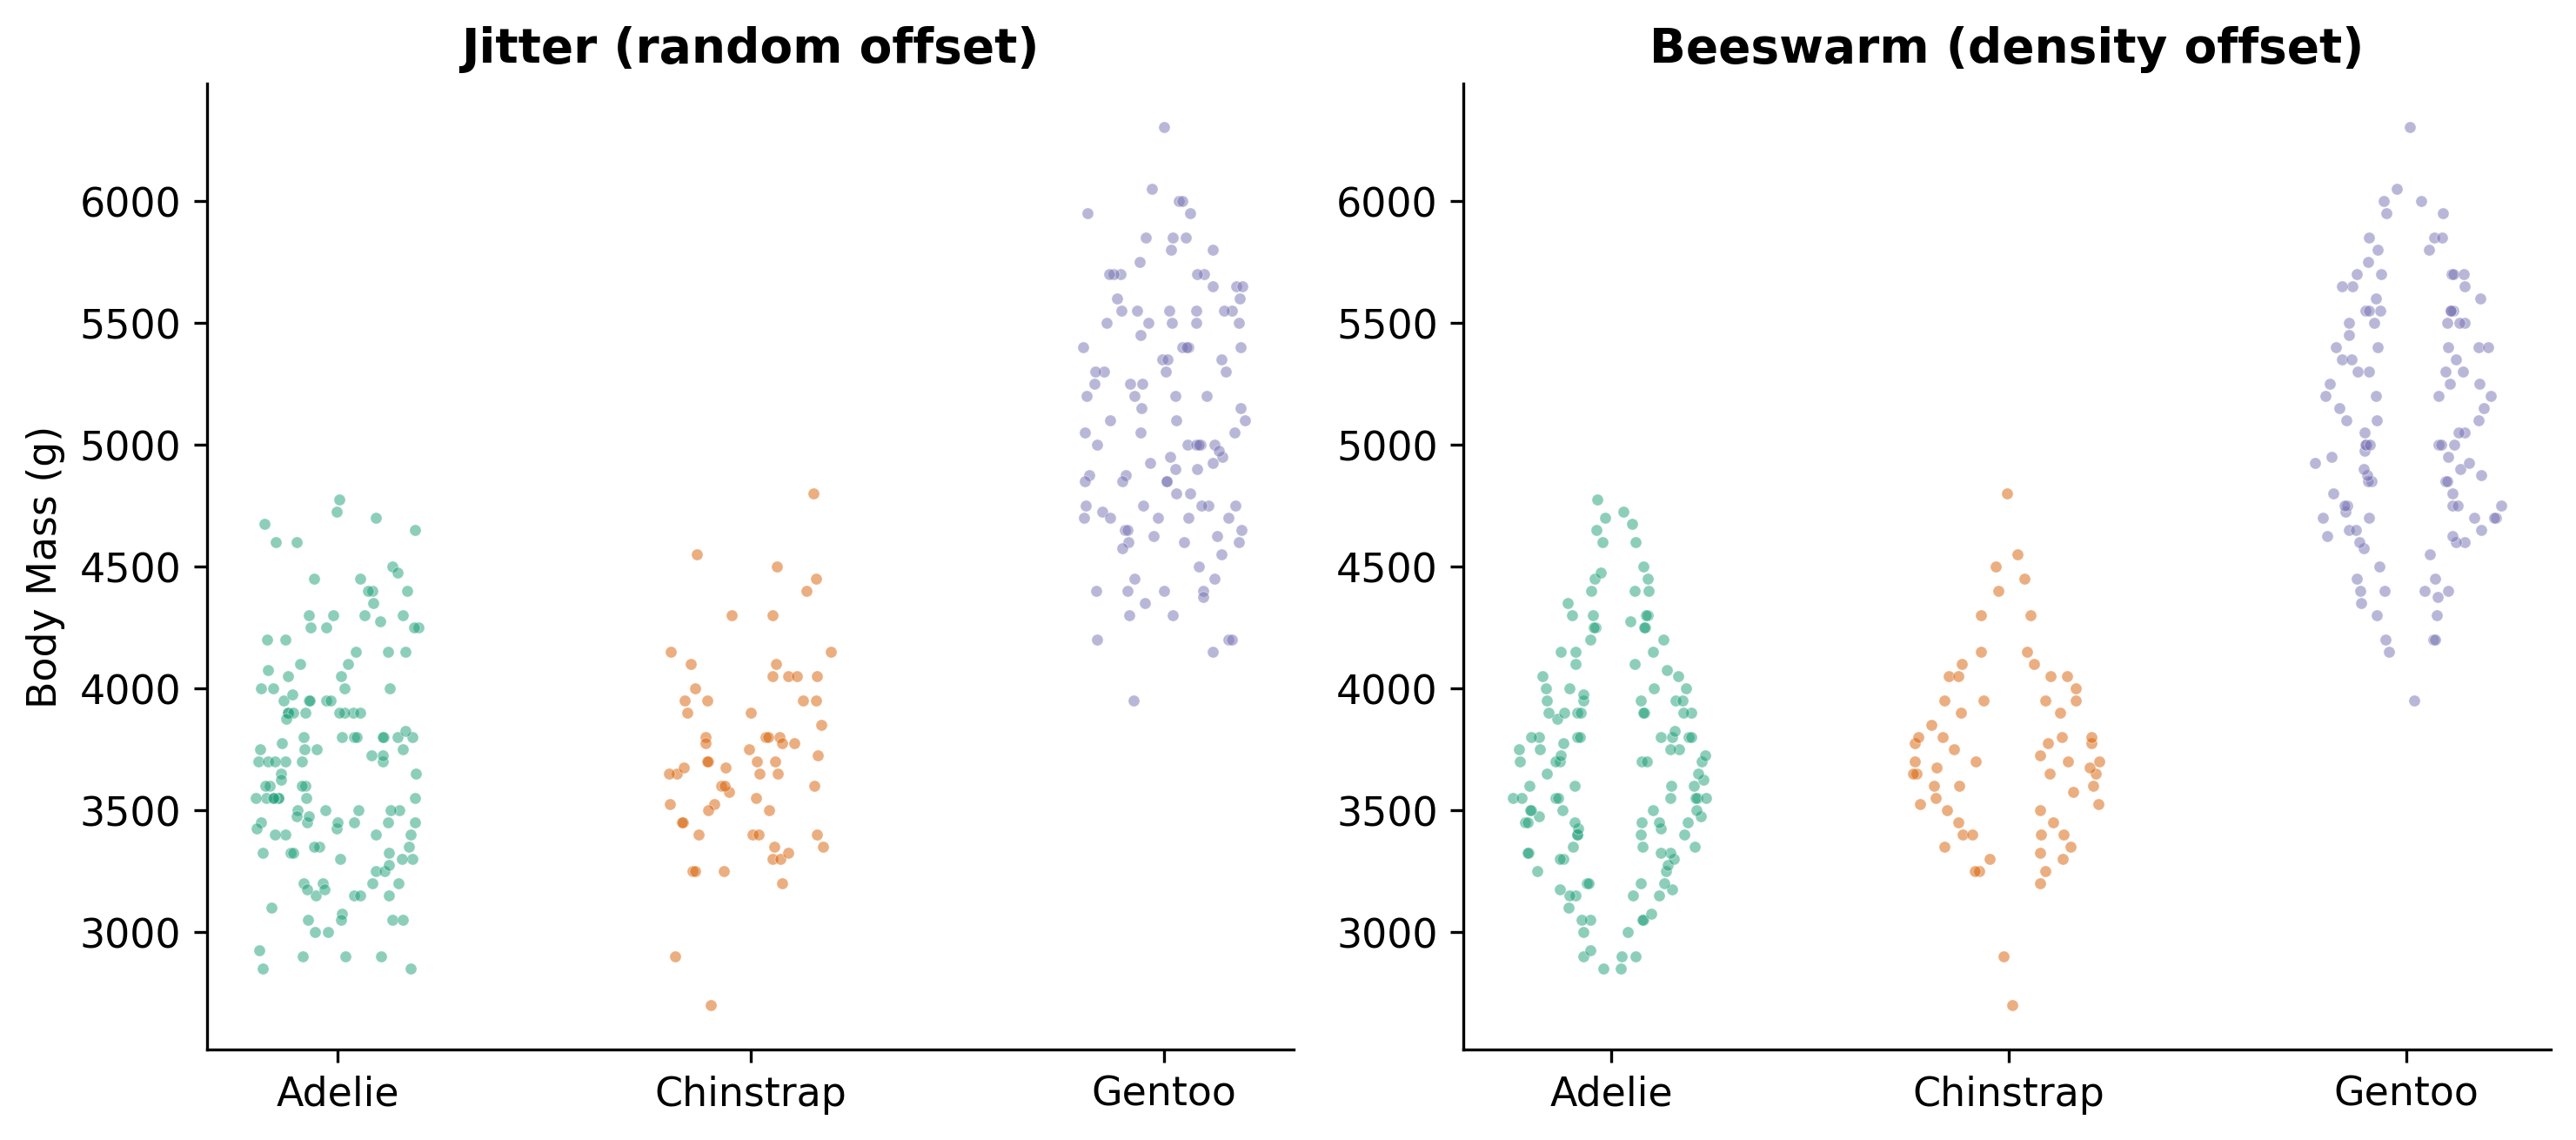
\includegraphics[width=0.85\textwidth]{m2_2_beeswarm.png}

\vspace{0.2cm}
\begin{columns}[T]
\begin{column}{0.48\textwidth}
\begin{exampleblock}{Data Insight}
    \scriptsize Left: random jitter wastes horizontal space. Right: beeswarm packs points using \textbf{density-dependent} offsets --- the horizontal spread reflects local density, like a built-in violin.
\end{exampleblock}
\end{column}
\begin{column}{0.48\textwidth}
\begin{alertblock}{Pro-Tip}
    \scriptsize Beeswarm is ideal for $n = 20$--$200$. Below 20, plain strip suffices. Above 200, points overlap even with beeswarm --- switch to violin.
\end{alertblock}
\end{column}
\end{columns}
\end{frame}

% ── 48 ──
\begin{frame}[fragile]{Beeswarm --- \Rlang}\smark{48/300}
\begin{columns}[T]
\begin{column}{0.55\textwidth}
\begin{lstlisting}[style=Rstyle]
# ggbeeswarm package
library(ggbeeswarm)

ggplot(penguins,
  aes(species, body_mass_g,
      color = species)) +
  geom_beeswarm(
    cex = 2, alpha = 0.6,
    size = 1.5) +
  theme_minimal() +
  theme(legend.position="none")

# Sina plot (violin-guided jitter)
ggplot(penguins,
  aes(species, body_mass_g)) +
  geom_sina(alpha = 0.5,
    size = 1.5)
\end{lstlisting}
\end{column}
\begin{column}{0.42\textwidth}
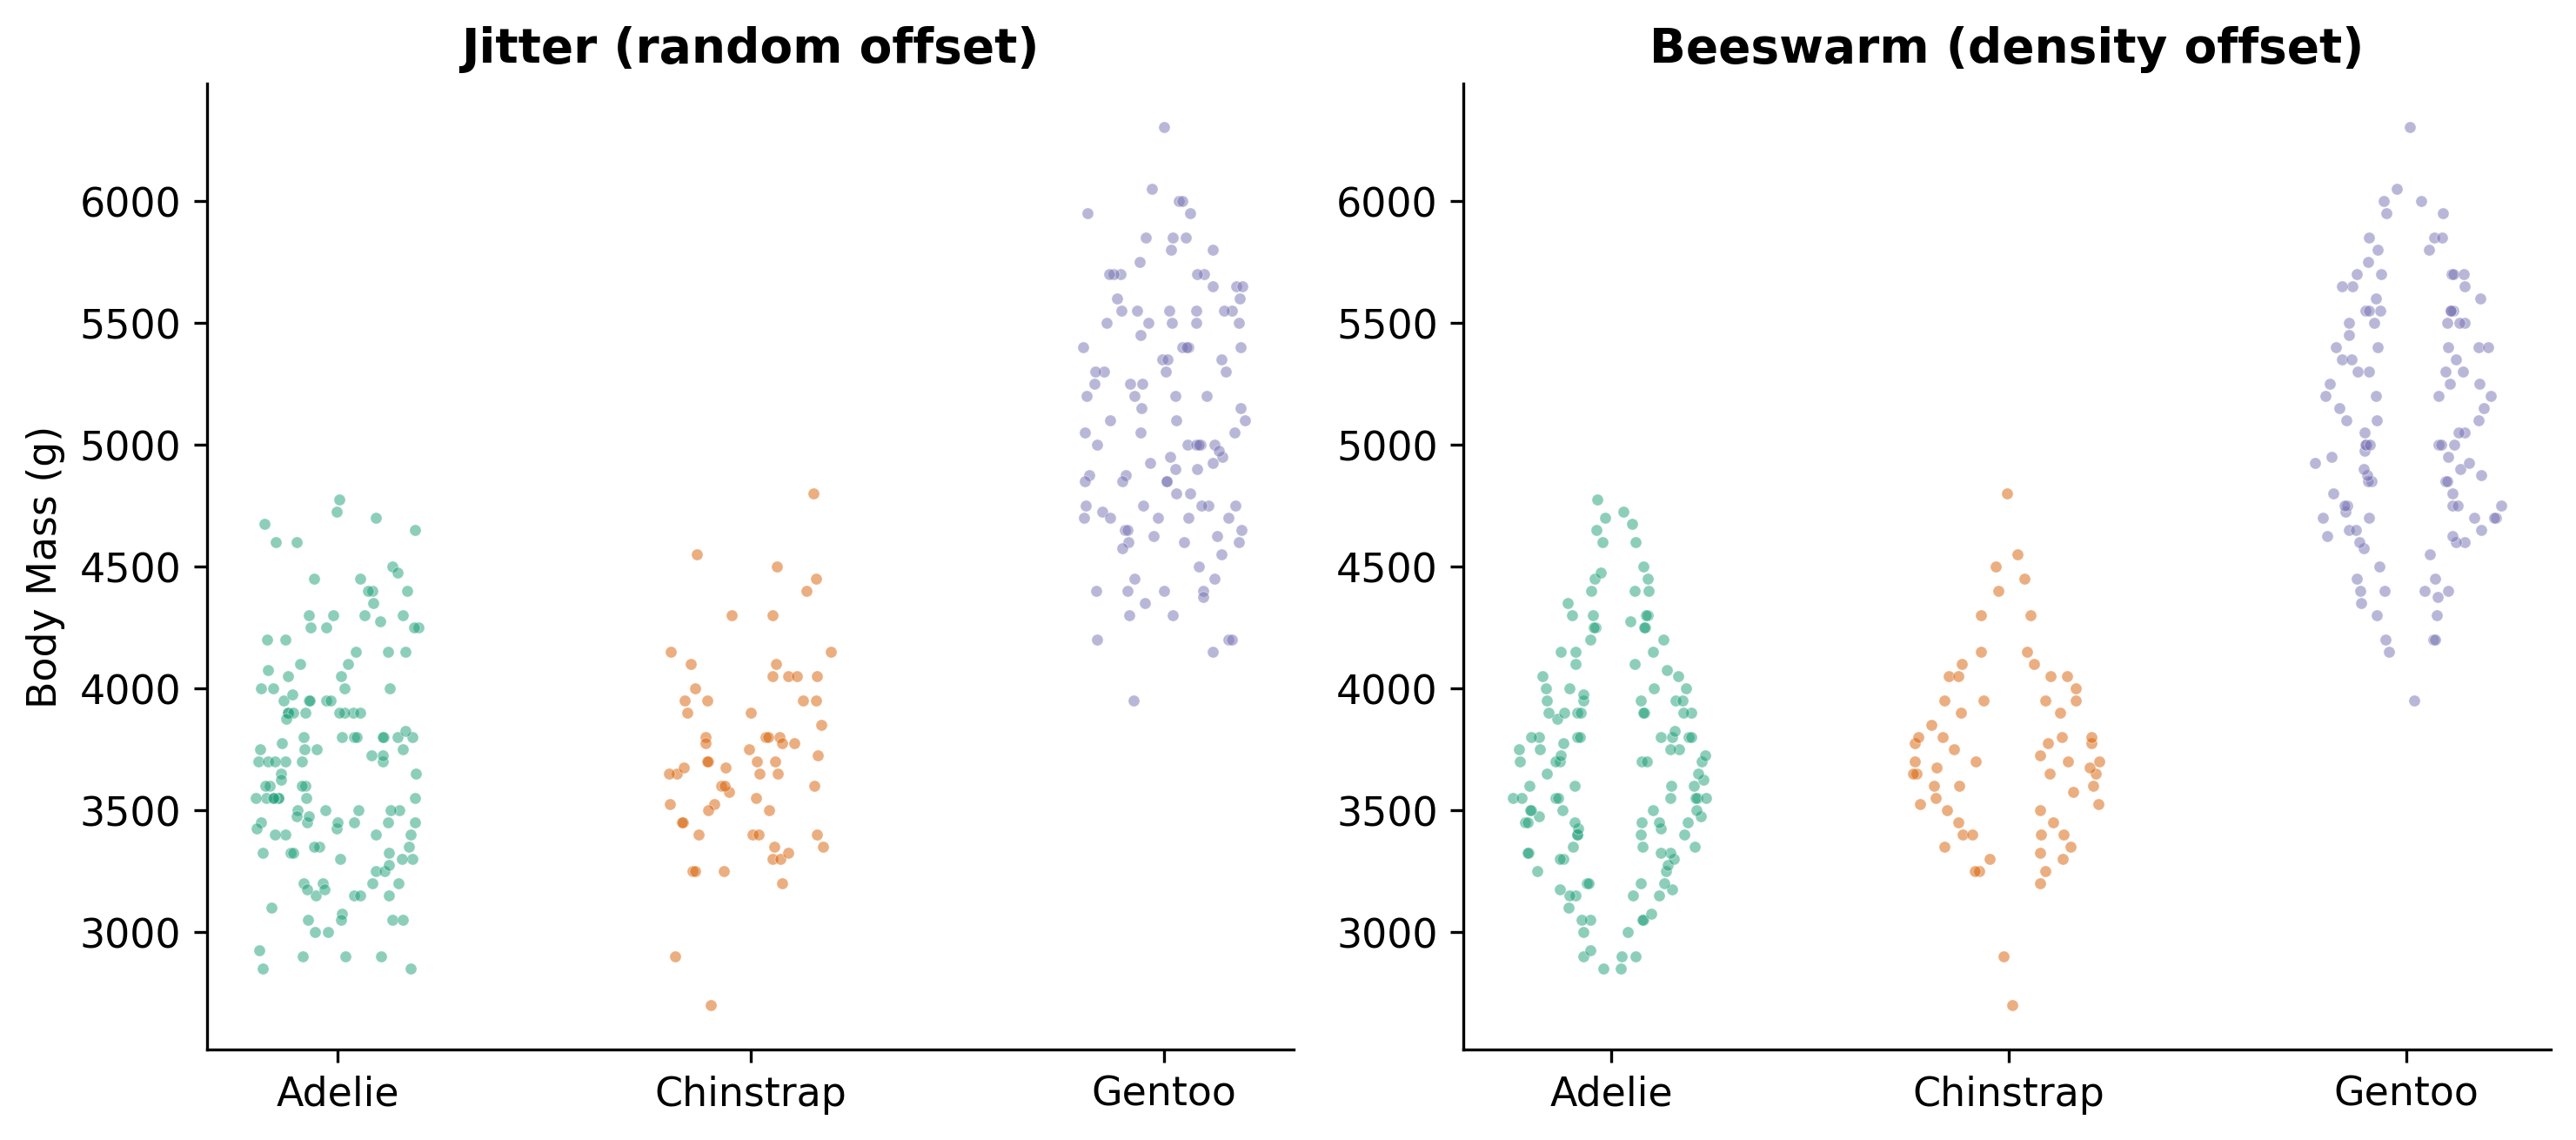
\includegraphics[width=\textwidth]{m2_2_beeswarm.png}
\begin{exampleblock}{Data Insight}
    \scriptsize \texttt{geom\_sina()} from \texttt{ggforce} is the ``violin-guided jitter'': point offsets are proportional to the local KDE density. It is a beeswarm that \emph{exactly} fills a violin shape.
\end{exampleblock}
\end{column}
\end{columns}
\end{frame}

% ── 49 ──
\begin{frame}[fragile]{Beeswarm --- \Python}\smark{49/300}
\begin{columns}[T]
\begin{column}{0.55\textwidth}
\begin{lstlisting}[style=Pystyle]
# seaborn swarmplot
sns.swarmplot(data=penguins,
    x="species", y="body_mass_g",
    hue="species",
    palette=["#1B9E77","#D95F02",
             "#7570B3"],
    size=3, alpha=0.6,
    legend=False)

# Combines with violin
fig, ax = plt.subplots()
sns.violinplot(data=penguins,
    x="species", y="body_mass_g",
    inner=None, alpha=0.2, ax=ax)
sns.swarmplot(data=penguins,
    x="species", y="body_mass_g",
    size=2, alpha=0.5, ax=ax,
    color="#333")
\end{lstlisting}
\end{column}
\begin{column}{0.42\textwidth}
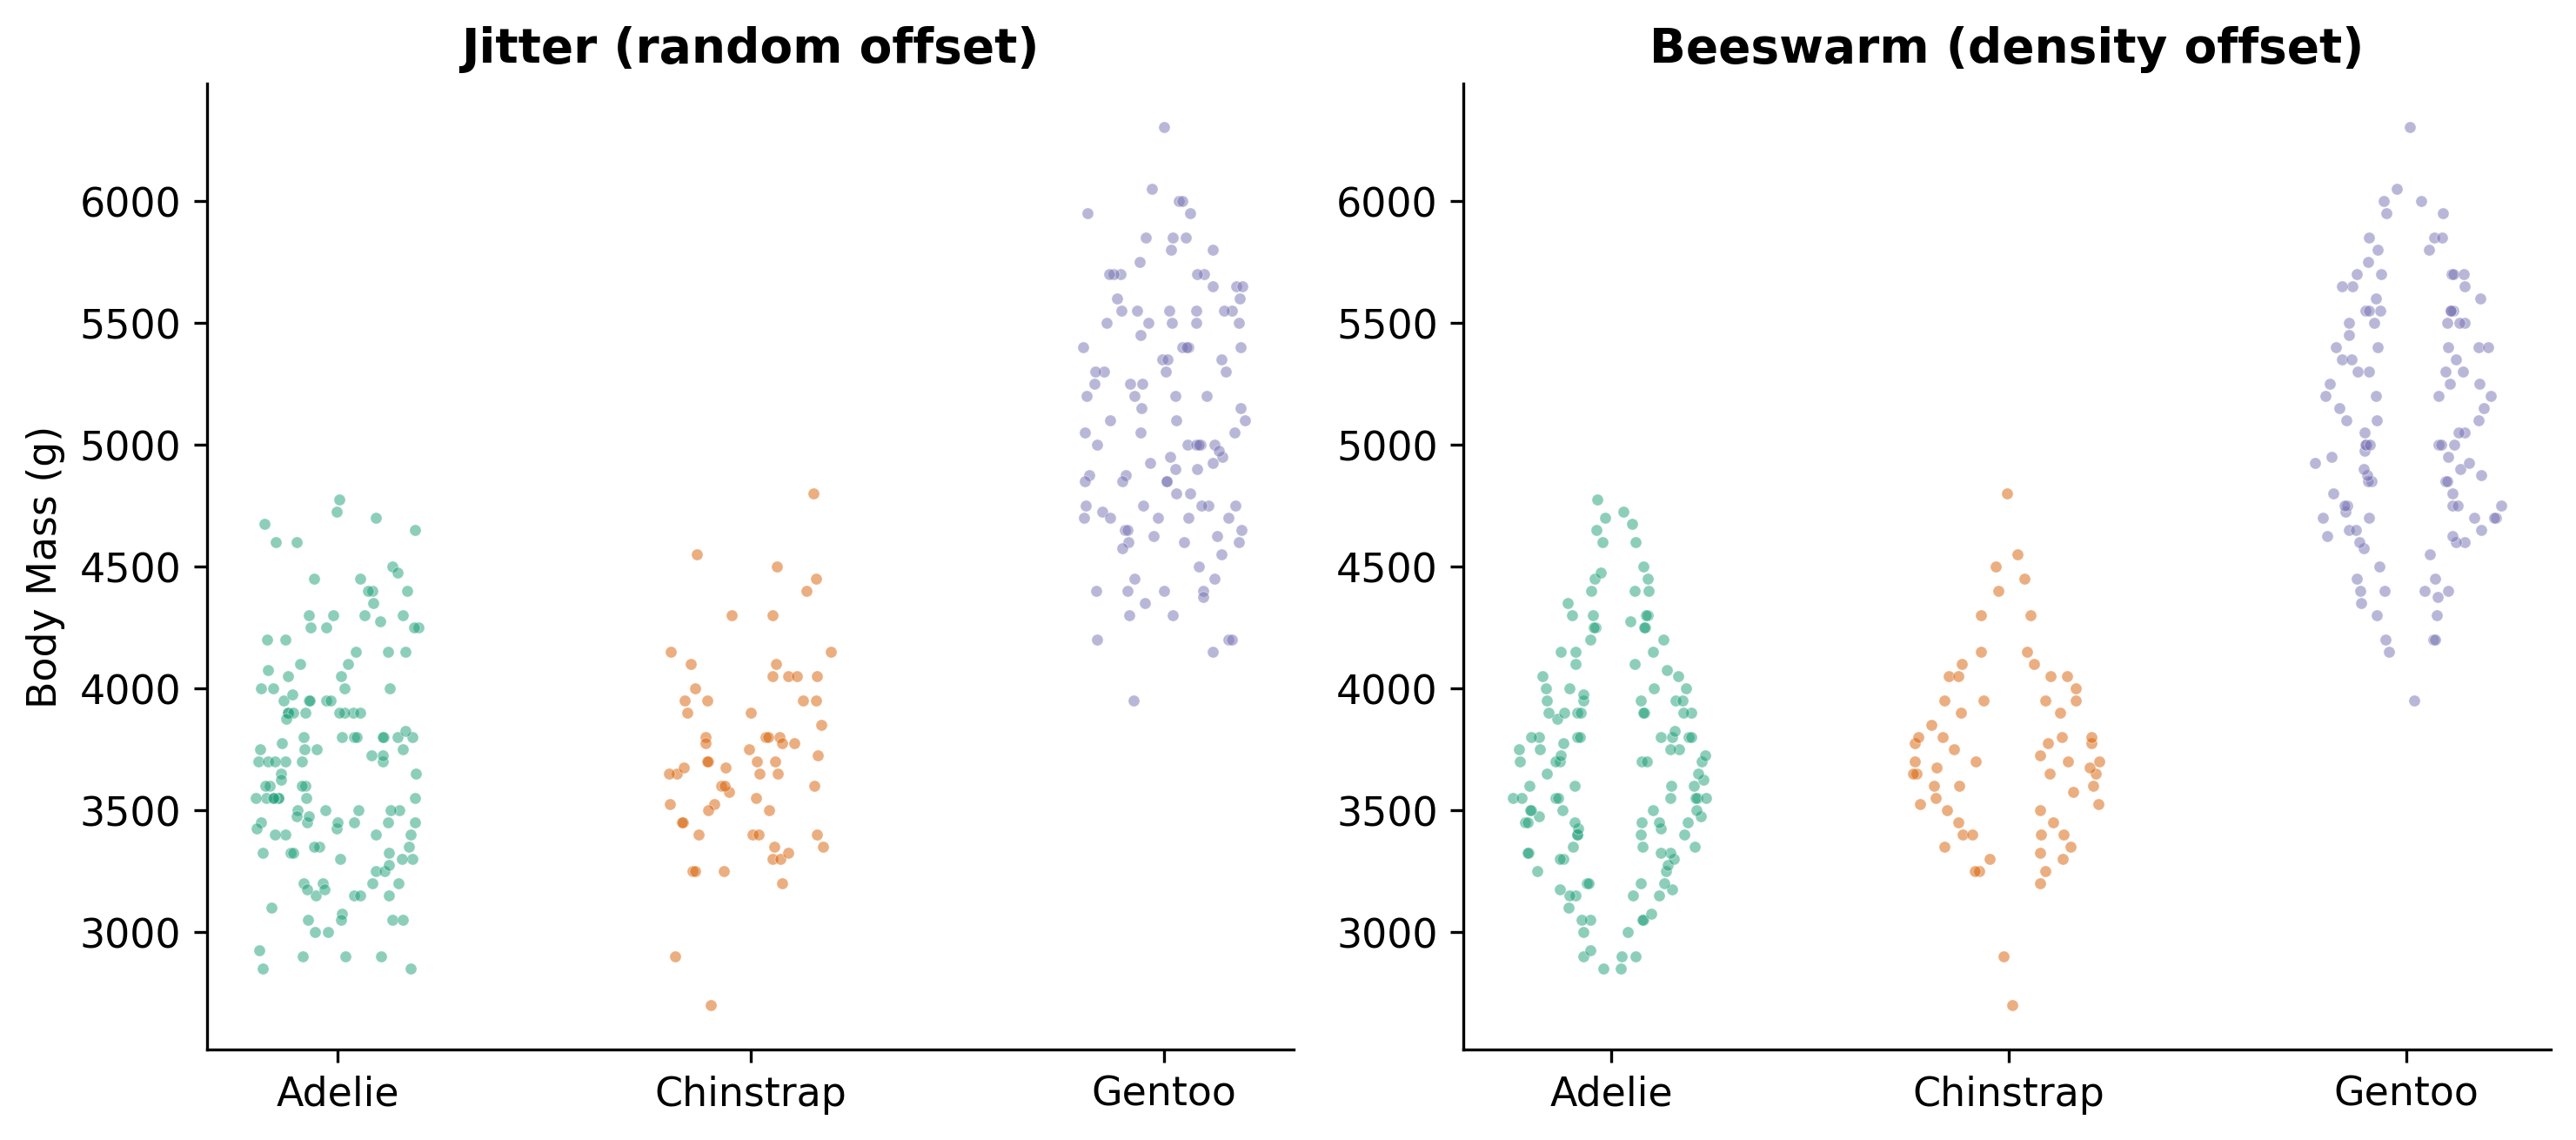
\includegraphics[width=\textwidth]{m2_2_beeswarm.png}
\begin{alertblock}{Pro-Tip}
    \scriptsize \texttt{swarmplot()} is seaborn's beeswarm. It can be \textbf{slow} for $n > 500$ (collision avoidance is $O(n^2)$). Use \texttt{stripplot()} for large $n$ and reserve swarm for small samples.
\end{alertblock}
\end{column}
\end{columns}
\end{frame}

% ── 50 ──
\begin{frame}{Grouped Violins: Splitting by a Second Variable}
\smark{50/300}
\begin{columns}[T]
\begin{column}{0.50\textwidth}
\begin{itemize}
    \item \textbf{Split violin}: two groups share one position, each taking half
    \item \textbf{Dodged violin}: side-by-side violins within each category
    \item Best for 2-level grouping (e.g., sex within species)
    \item Becomes unreadable at 3+ levels
\end{itemize}
\end{column}
\begin{column}{0.47\textwidth}
\begin{alertblock}{Pro-Tip}
    \scriptsize In ggplot2: \texttt{geom\_violin(position="dodge")}. For split violins: \texttt{geom\_split\_violin()} from \texttt{introdataviz} package, or use \texttt{see::geom\_violindot()}.
\end{alertblock}
\vspace{0.2cm}
\begin{exampleblock}{Data Insight}
    \scriptsize In seaborn: \texttt{sns.violinplot(hue="sex", split=True)}. The \texttt{split=True} parameter creates the half-and-half layout automatically.
\end{exampleblock}
\end{column}
\end{columns}
\end{frame}

% ── 51 ──
\begin{frame}[fragile]{Grouped Violins --- Code}\smark{51/300}
\begin{columns}[T]
\begin{column}{0.48\textwidth}
\begin{lstlisting}[style=Rstyle]
# Dodged
ggplot(penguins,
  aes(species, body_mass_g,
      fill = sex)) +
  geom_violin(
    position = "dodge",
    alpha = 0.4) +
  theme_minimal()

# Split (seaborn-style)
# Requires introdataviz or see
library(see)
ggplot(penguins,
  aes(species, body_mass_g,
      fill = sex)) +
  geom_violindot(
    fill_dots = "grey") +
  theme_modern()
\end{lstlisting}
\end{column}
\begin{column}{0.48\textwidth}
\begin{lstlisting}[style=Pystyle]
# seaborn split violin
sns.violinplot(data=penguins,
    x="species",
    y="body_mass_g",
    hue="sex",
    split=True,
    inner="quartile",
    palette=["#2166AC","#B2182B"])

# Dodged (default when split=False)
sns.violinplot(data=penguins,
    x="species",
    y="body_mass_g",
    hue="sex",
    split=False)
\end{lstlisting}
\end{column}
\end{columns}
\end{frame}

% ── 52 ──
\begin{frame}{Notched Boxplots: Quick Inference}
\smark{52/300}
\begin{columns}[T]
\begin{column}{0.50\textwidth}
\begin{itemize}
    \item Notch at the median $\pm 1.58 \times \text{IQR} / \sqrt{n}$
    \item Approximate 95\% CI for the median
    \item Non-overlapping notches $\Rightarrow$ medians are ``significantly different''
    \item Quick visual test without running a formal procedure
\end{itemize}
\end{column}
\begin{column}{0.47\textwidth}
\begin{alertblock}{Pro-Tip}
    \scriptsize R: \texttt{geom\_boxplot(notch=TRUE)}. Python: \texttt{sns.boxplot(notch=True)} or \texttt{ax.boxplot(notch=True)}. If the notch extends beyond the box, the CI is wider than the IQR --- interpret with caution.
\end{alertblock}
\vspace{0.2cm}
\begin{exampleblock}{Data Insight}
    \scriptsize Notched boxplots are the poor man's $t$-test visual. Useful in exploratory work; for publication, report formal CIs or posterior intervals.
\end{exampleblock}
\end{column}
\end{columns}
\end{frame}

% ── 53 ──
\begin{frame}[fragile]{Notched Boxplot --- Code}\smark{53/300}
\begin{columns}[T]
\begin{column}{0.48\textwidth}
\begin{lstlisting}[style=Rstyle]
ggplot(penguins,
  aes(species, body_mass_g,
      fill = species)) +
  geom_boxplot(notch = TRUE,
    alpha = 0.5) +
  theme_minimal() +
  theme(legend.position="none")
\end{lstlisting}
\end{column}
\begin{column}{0.48\textwidth}
\begin{lstlisting}[style=Pystyle]
sns.boxplot(data=penguins,
    x="species", y="body_mass_g",
    notch=True,
    palette=["#1B9E77","#D95F02",
             "#7570B3"])

# matplotlib
ax.boxplot(data_list,
    notch=True,
    patch_artist=True)
\end{lstlisting}
\end{column}
\end{columns}
\end{frame}

% ── 54 ──
\begin{frame}{Letter-Value Plots for Large $n$}
\smark{54/300}
\centering
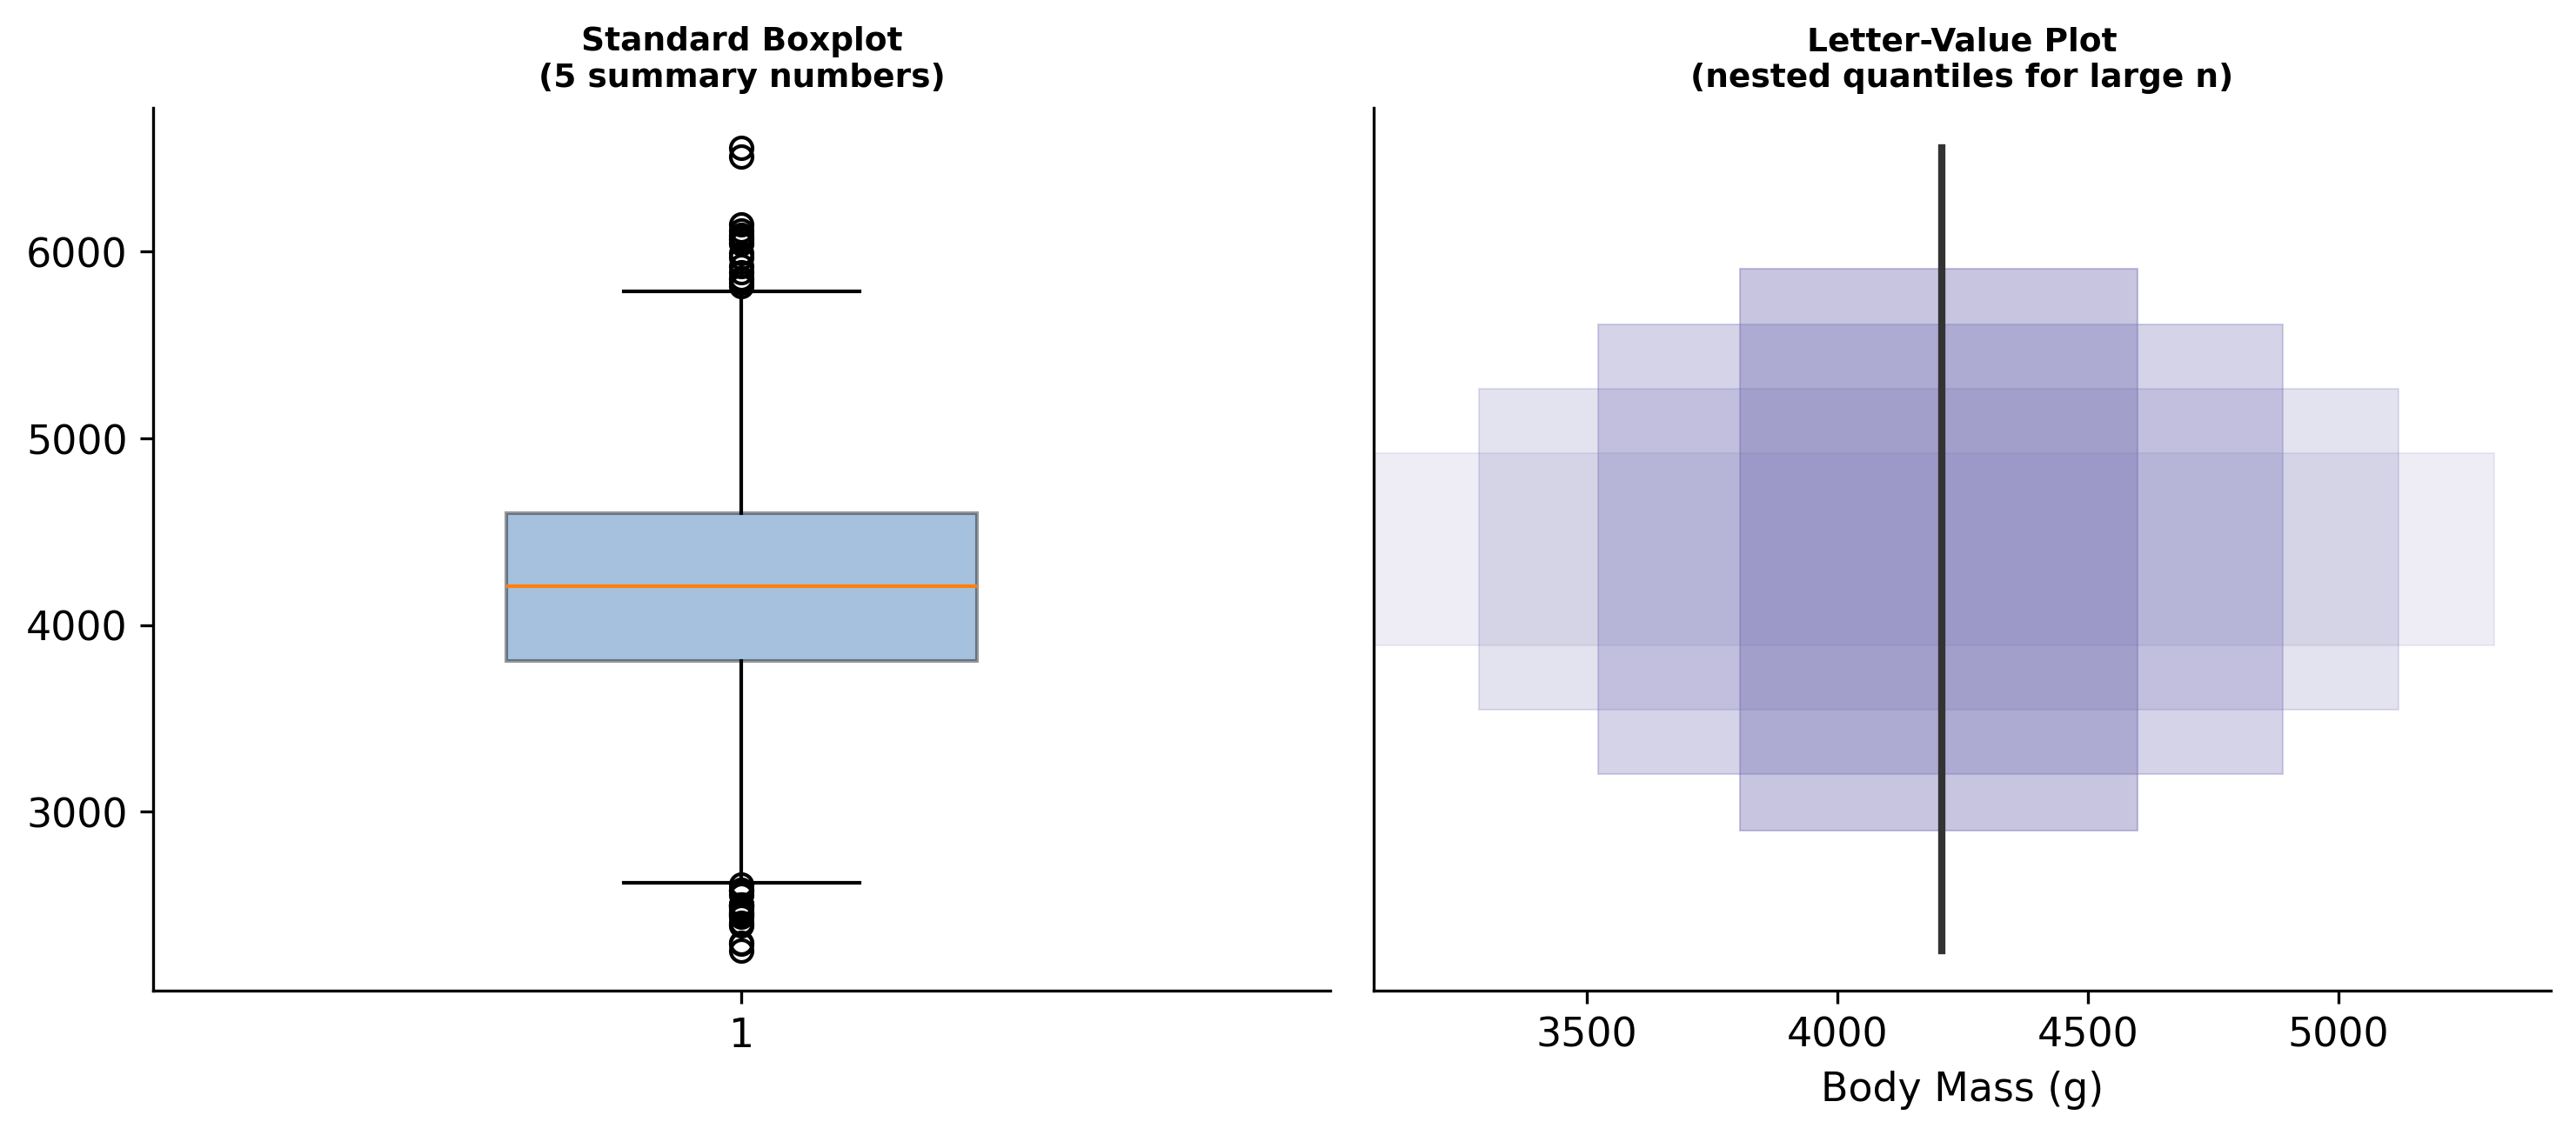
\includegraphics[width=0.85\textwidth]{m2_2_lettervalue.png}

\vspace{0.2cm}
\begin{columns}[T]
\begin{column}{0.48\textwidth}
\begin{itemize}
    \item Standard boxplot uses 5 values regardless of $n$
    \item Letter-value plots add nested quantiles: eighths, sixteenths\ldots
    \item More detail in the tails for large $n$
    \item Hofmann et al.\ (2017)
\end{itemize}
\end{column}
\begin{column}{0.48\textwidth}
\begin{alertblock}{Pro-Tip}
    \scriptsize R: \texttt{ggplot2::geom\_boxplot()} cannot do this; use \texttt{lvplot::geom\_lv()}. Python: \texttt{sns.boxenplot()} (seaborn's name for letter-value). Best for $n > 1{,}000$.
\end{alertblock}
\end{column}
\end{columns}
\end{frame}

% ── 55 ──
\begin{frame}[fragile]{Letter-Value / Boxen Plot --- Code}\smark{55/300}
\begin{columns}[T]
\begin{column}{0.48\textwidth}
\begin{lstlisting}[style=Rstyle]
library(lvplot)

ggplot(diamonds,
  aes(cut, price,
      fill = cut)) +
  geom_lv(alpha = 0.5) +
  theme_minimal() +
  theme(legend.position="none")
# Each nested box = one
# more quantile level
\end{lstlisting}
\end{column}
\begin{column}{0.48\textwidth}
\begin{lstlisting}[style=Pystyle]
# seaborn boxenplot
sns.boxenplot(data=diamonds,
    x="cut", y="price",
    palette="Set2")

# k_depth controls nesting
sns.boxenplot(data=diamonds,
    x="cut", y="price",
    k_depth="trustworthy")
# Options: "tukey", "proportion",
# "trustworthy", "full"
\end{lstlisting}
\vspace{0.1cm}
\begin{exampleblock}{Data Insight}
    \scriptsize \texttt{k\_depth="trustworthy"} adds quantile boxes only where the sample size gives reliable estimates. Prevents over-detailing in small groups.
\end{exampleblock}
\end{column}
\end{columns}
\end{frame}

% ── 56 ──
\begin{frame}{Horizontal Orientation for Distribution Plots}
\smark{56/300}
\begin{columns}[T]
\begin{column}{0.50\textwidth}
\begin{itemize}
    \item \texttt{coord\_flip()} works for all distribution geoms
    \item Horizontal layout: categories on $y$-axis, values on $x$
    \item Better for long category labels
    \item Rainclouds look best horizontal (gravity metaphor)
\end{itemize}
\end{column}
\begin{column}{0.47\textwidth}
\begin{alertblock}{Pro-Tip}
    \scriptsize In seaborn: \texttt{orient="h"} for most cat plots. In ggplot2 v3.3+: swap \texttt{aes(x=, y=)} directly or use \texttt{coord\_flip()}. In plotnine: \texttt{coord\_flip()} is the reliable approach.
\end{alertblock}
\end{column}
\end{columns}
\end{frame}

% ── 57 ──
\begin{frame}{Ridgeline Plots: Faceted Density}
\smark{57/300}
\begin{columns}[T]
\begin{column}{0.50\textwidth}
\begin{itemize}
    \item Stacked density plots with slight overlap
    \item Each group gets its own ``ridge''
    \item Excellent for many groups (10--30)
    \item Popularized by the Joy Division album cover
    \item R: \texttt{ggridges::geom\_density\_ridges}
    \item Python: \texttt{joypy} or manual with subplots
\end{itemize}
\end{column}
\begin{column}{0.47\textwidth}
\begin{exampleblock}{Data Insight}
    \scriptsize Ridgelines scale where violins don't. 20 violins side-by-side are too thin; 20 ridgelines stacked vertically remain readable because each occupies a full row.
\end{exampleblock}
\vspace{0.2cm}
\begin{alertblock}{Pro-Tip}
    \scriptsize Overlap with \texttt{scale=1.2} in \texttt{ggridges}. Too much overlap hides lower ridges; too little wastes space.
\end{alertblock}
\end{column}
\end{columns}
\end{frame}

% ── 58 ──
\begin{frame}[fragile]{Ridgeline --- Code}\smark{58/300}
\begin{columns}[T]
\begin{column}{0.48\textwidth}
\begin{lstlisting}[style=Rstyle]
library(ggridges)

ggplot(penguins,
  aes(body_mass_g, species,
      fill = species)) +
  geom_density_ridges(
    alpha = 0.4, scale = 1.2) +
  theme_minimal() +
  theme(legend.position="none")

# With quantile lines
geom_density_ridges(
  quantile_lines = TRUE,
  quantiles = c(0.25, 0.5, 0.75))
\end{lstlisting}
\end{column}
\begin{column}{0.48\textwidth}
\begin{lstlisting}[style=Pystyle]
# pip install joypy
import joypy

fig, axes = joypy.joyplot(
    penguins,
    by="species",
    column="body_mass_g",
    colormap=plt.cm.Set2,
    alpha=0.5, overlap=0.4)
plt.xlabel("Body Mass (g)")

# plotnine: geom_density_ridges
# via plotnine_prism or manual
\end{lstlisting}
\end{column}
\end{columns}
\end{frame}

% ── 59 ──
\begin{frame}{Distribution Plot Decision Guide}
\smark{59/300}
\centering\small
\begin{tabular}{@{}llll@{}}
    \toprule
    \textbf{$n$ per group} & \textbf{Groups} & \textbf{Goal} & \textbf{Best Plot} \\
    \midrule
    $< 10$        & 2--5    & Show every point        & Strip only \\
    $10$--$50$    & 2--5    & Shape + raw data        & Raincloud or hybrid \\
    $50$--$200$   & 2--5    & Shape + summary         & Violin + box \\
    $> 200$       & 2--5    & Shape                   & Violin or letter-value \\
    Any           & 2--5    & Quick inference         & Notched boxplot \\
    Any           & 5--30   & Compare many groups     & Ridgeline \\
    $20$--$200$   & 2--5    & Non-overlapping points  & Beeswarm \\
    \bottomrule
\end{tabular}

\vspace{0.3cm}
\begin{exampleblock}{Data Insight}
    \scriptsize No single plot type is universally best. The decision depends on $n$, the number of groups, and whether you prioritize raw data display or summary comparison.
\end{exampleblock}
\end{frame}

% ── 60 ──
\begin{frame}{Module 2.2 --- Key Takeaways}\smark{60/300}
\begin{enumerate}
    \item \textbf{Boxplots hide bimodality.} Never use them alone.
    \item \textbf{Violins show shape.} Pair with box or strip for summary.
    \item \textbf{Rainclouds} = half-violin + box + strip: maximum information density.
    \item \textbf{Beeswarm} packs points by density: ideal for $20 \leq n \leq 200$.
    \item \textbf{Letter-value plots} for large $n$ ($> 1{,}000$).
    \item \textbf{Ridgelines} scale to 10--30 groups where violins fail.
\end{enumerate}
\end{frame}

% ── 61 ──
\begin{frame}{}\smark{61/300}
\centering\vspace{1.5cm}
{\Large\textbf{Module 2.2 Complete}}\\[0.5cm]
You now have the full distribution visualization toolkit: boxplot, violin, raincloud, beeswarm, ridgeline, and letter-value --- and know when to deploy each.\\[0.5cm]
\textbf{Next:} Module 2.3 --- Regression Diagnostics and Model Visualization.
\end{frame}

% % ═══════════════════════════════════════════════════════
%  MODULE 2.3 — Regression Diagnostics and Model Visualization
% ═══════════════════════════════════════════════════════
\section{Module 2.3 --- Regression Diagnostics and Model Visualization}

% ── 62 ──
\begin{frame}{Module 2.3 --- Roadmap}\smark{62/300}
\begin{enumerate}
    \item Scatter + regression line + confidence band
    \item Confidence interval vs.\ prediction interval
    \item The classic 4-panel diagnostic (\texttt{plot(lm)})
    \item Residuals vs.\ fitted: reading the pattern
    \item Heteroscedasticity: the funnel shape
    \item Cook's distance and influential points
    \item Partial regression and component-residual plots
    \item Smoother comparison: lm, loess, robust
\end{enumerate}
\end{frame}

% ── 63 ──
\begin{frame}{Scatter + Regression Line + CI Band}
\smark{63/300}
\centering
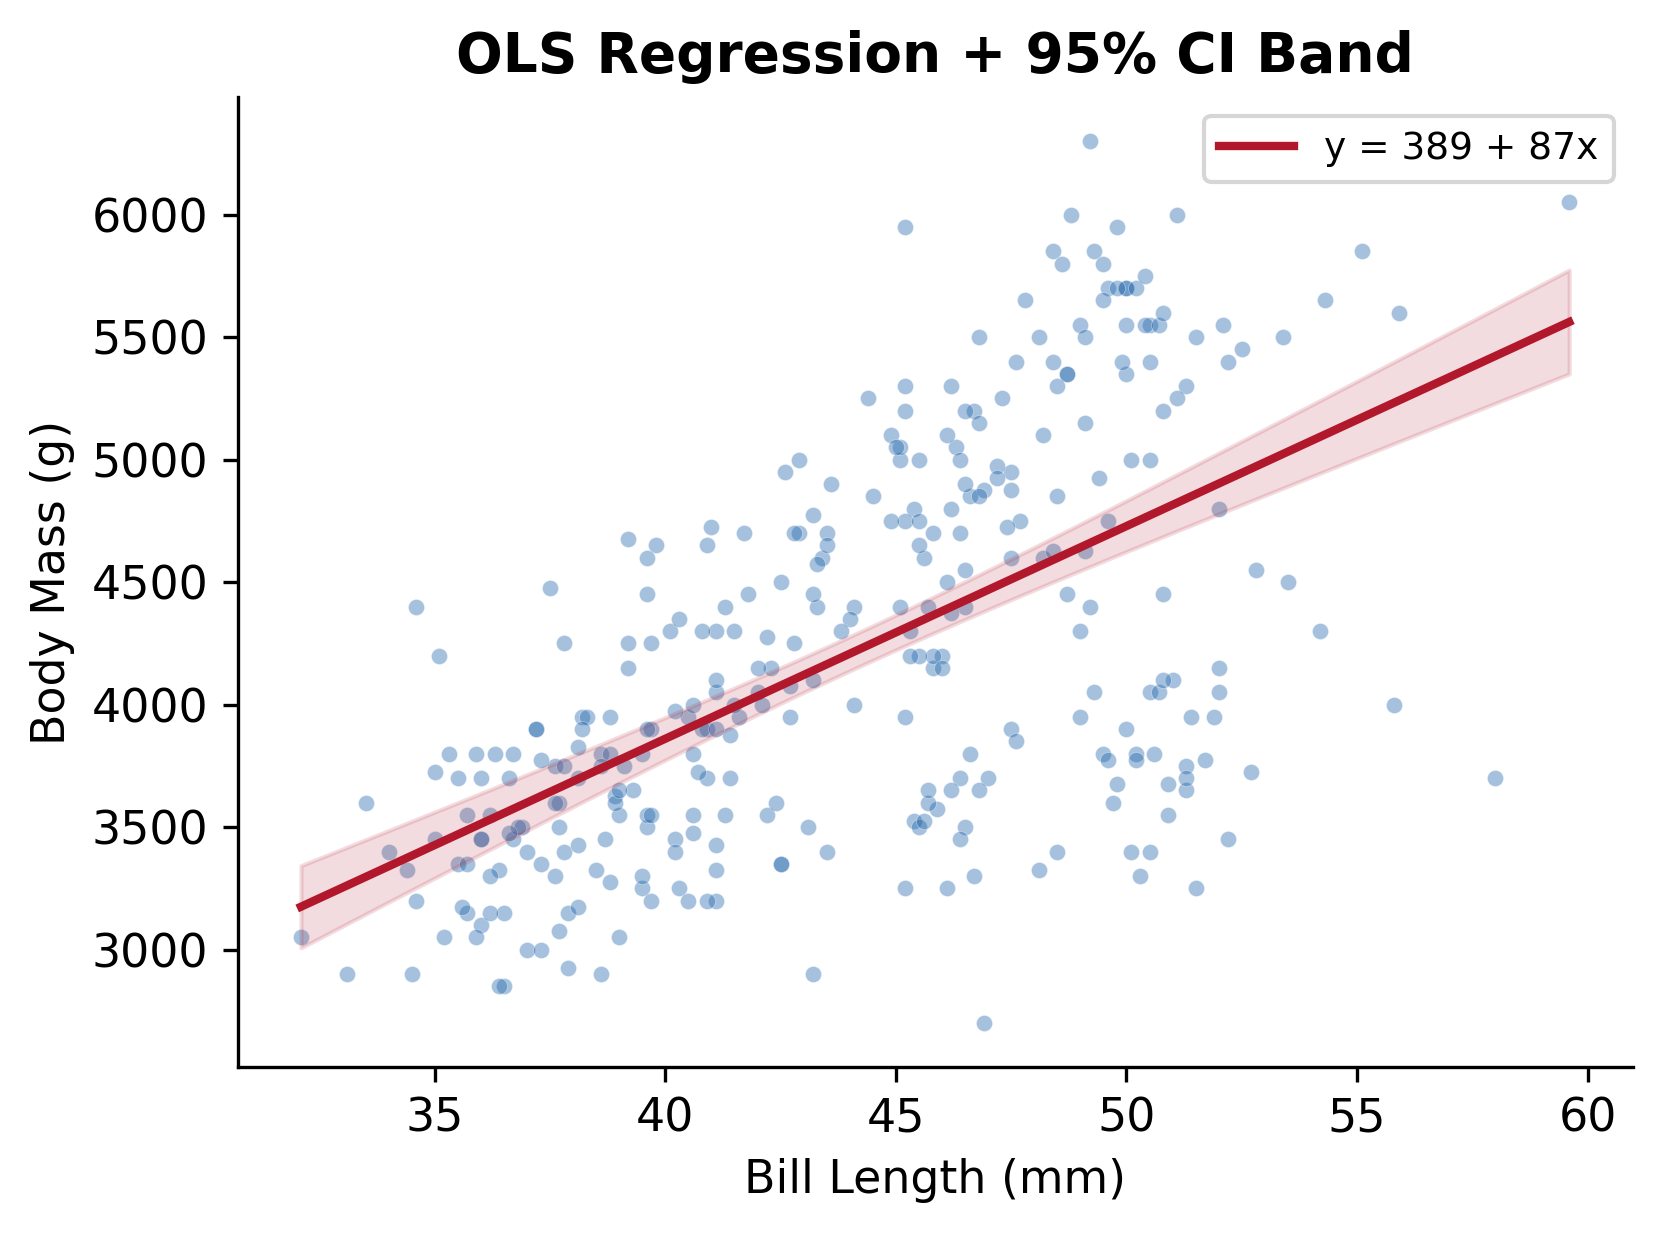
\includegraphics[width=0.68\textwidth]{m2_3_regression_ci.png}

\vspace{0.2cm}
\begin{columns}[T]
\begin{column}{0.48\textwidth}
\begin{exampleblock}{Data Insight}
    \scriptsize The blue band is the 95\% CI for the \textbf{mean} response. It narrows at $\bar{x}$ and widens at the extremes --- reflecting greater uncertainty in extrapolation.
\end{exampleblock}
\end{column}
\begin{column}{0.48\textwidth}
\begin{alertblock}{Pro-Tip}
    \scriptsize \texttt{geom\_smooth(method="lm")} adds the OLS line + CI in one layer. The default is \texttt{method="loess"} --- always specify the method explicitly.
\end{alertblock}
\end{column}
\end{columns}
\end{frame}

% ── 64 ──
\begin{frame}[fragile]{Regression + CI --- \Rlang}\smark{64/300}
\begin{columns}[T]
\begin{column}{0.55\textwidth}
\begin{lstlisting}[style=Rstyle]
ggplot(penguins,
  aes(bill_length_mm,
      body_mass_g)) +
  geom_point(alpha = 0.4,
    color = "#2166AC") +
  geom_smooth(method = "lm",
    color = "#B2182B",
    fill = "#B2182B",
    alpha = 0.15) +
  labs(x = "Bill Length (mm)",
       y = "Body Mass (g)") +
  theme_minimal()

# se=FALSE removes band
# formula = y ~ poly(x,2)
#   for quadratic
\end{lstlisting}
\end{column}
\begin{column}{0.42\textwidth}
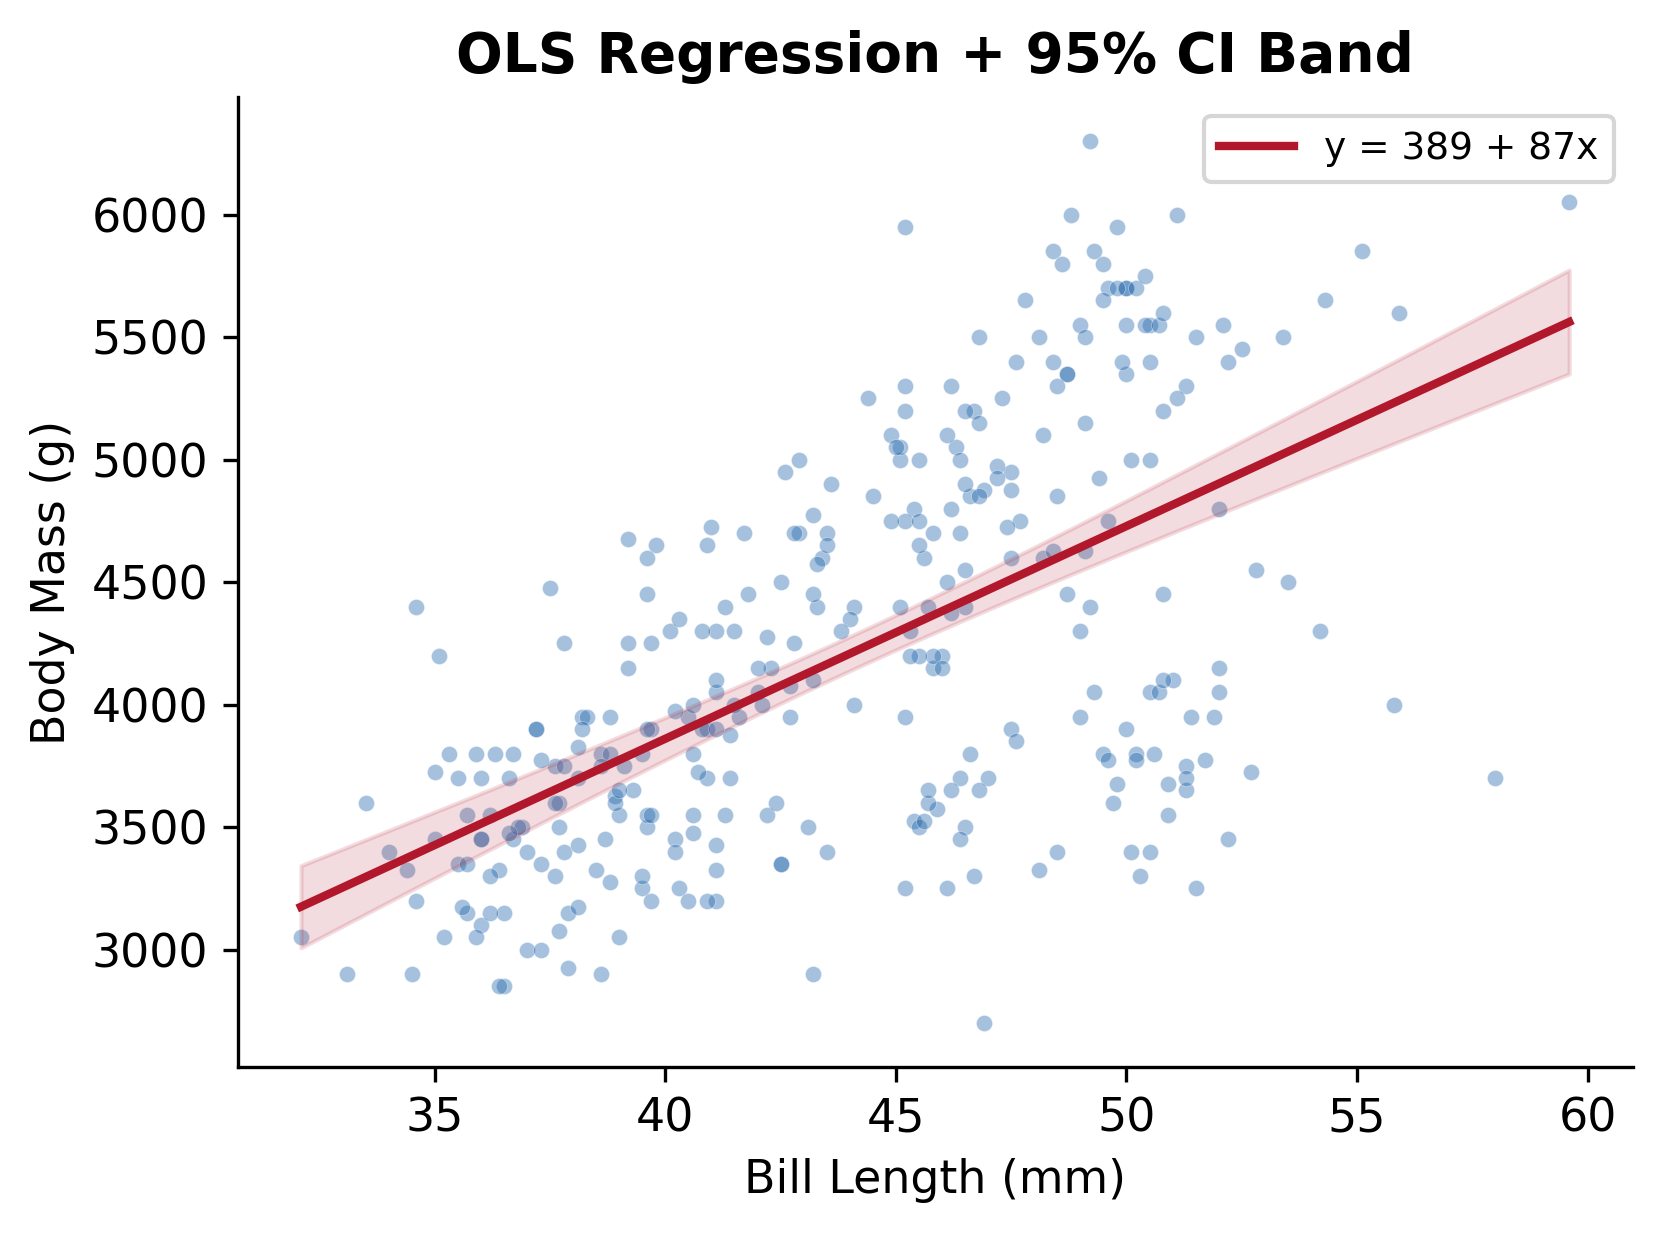
\includegraphics[width=\textwidth]{m2_3_regression_ci.png}
\begin{alertblock}{Pro-Tip}
    \scriptsize \texttt{geom\_smooth()} computes and plots the fit \emph{inside} ggplot2. For more control, fit with \texttt{lm()} first, then use \texttt{geom\_line(data=predictions)}.
\end{alertblock}
\end{column}
\end{columns}
\end{frame}

% ── 65 ──
\begin{frame}[fragile]{Regression + CI --- \Python}\smark{65/300}
\begin{columns}[T]
\begin{column}{0.55\textwidth}
\begin{lstlisting}[style=Pystyle]
# plotnine
(ggplot(penguins,
   aes("bill_length_mm",
       "body_mass_g"))
 + geom_point(alpha=0.4,
     color="#2166AC")
 + geom_smooth(method="lm",
     color="#B2182B",
     fill="#B2182B", alpha=0.15))

# seaborn regplot
sns.regplot(data=penguins,
    x="bill_length_mm",
    y="body_mass_g",
    ci=95,
    scatter_kws=dict(alpha=0.4,s=15),
    line_kws=dict(color="#B2182B"))
\end{lstlisting}
\end{column}
\begin{column}{0.42\textwidth}
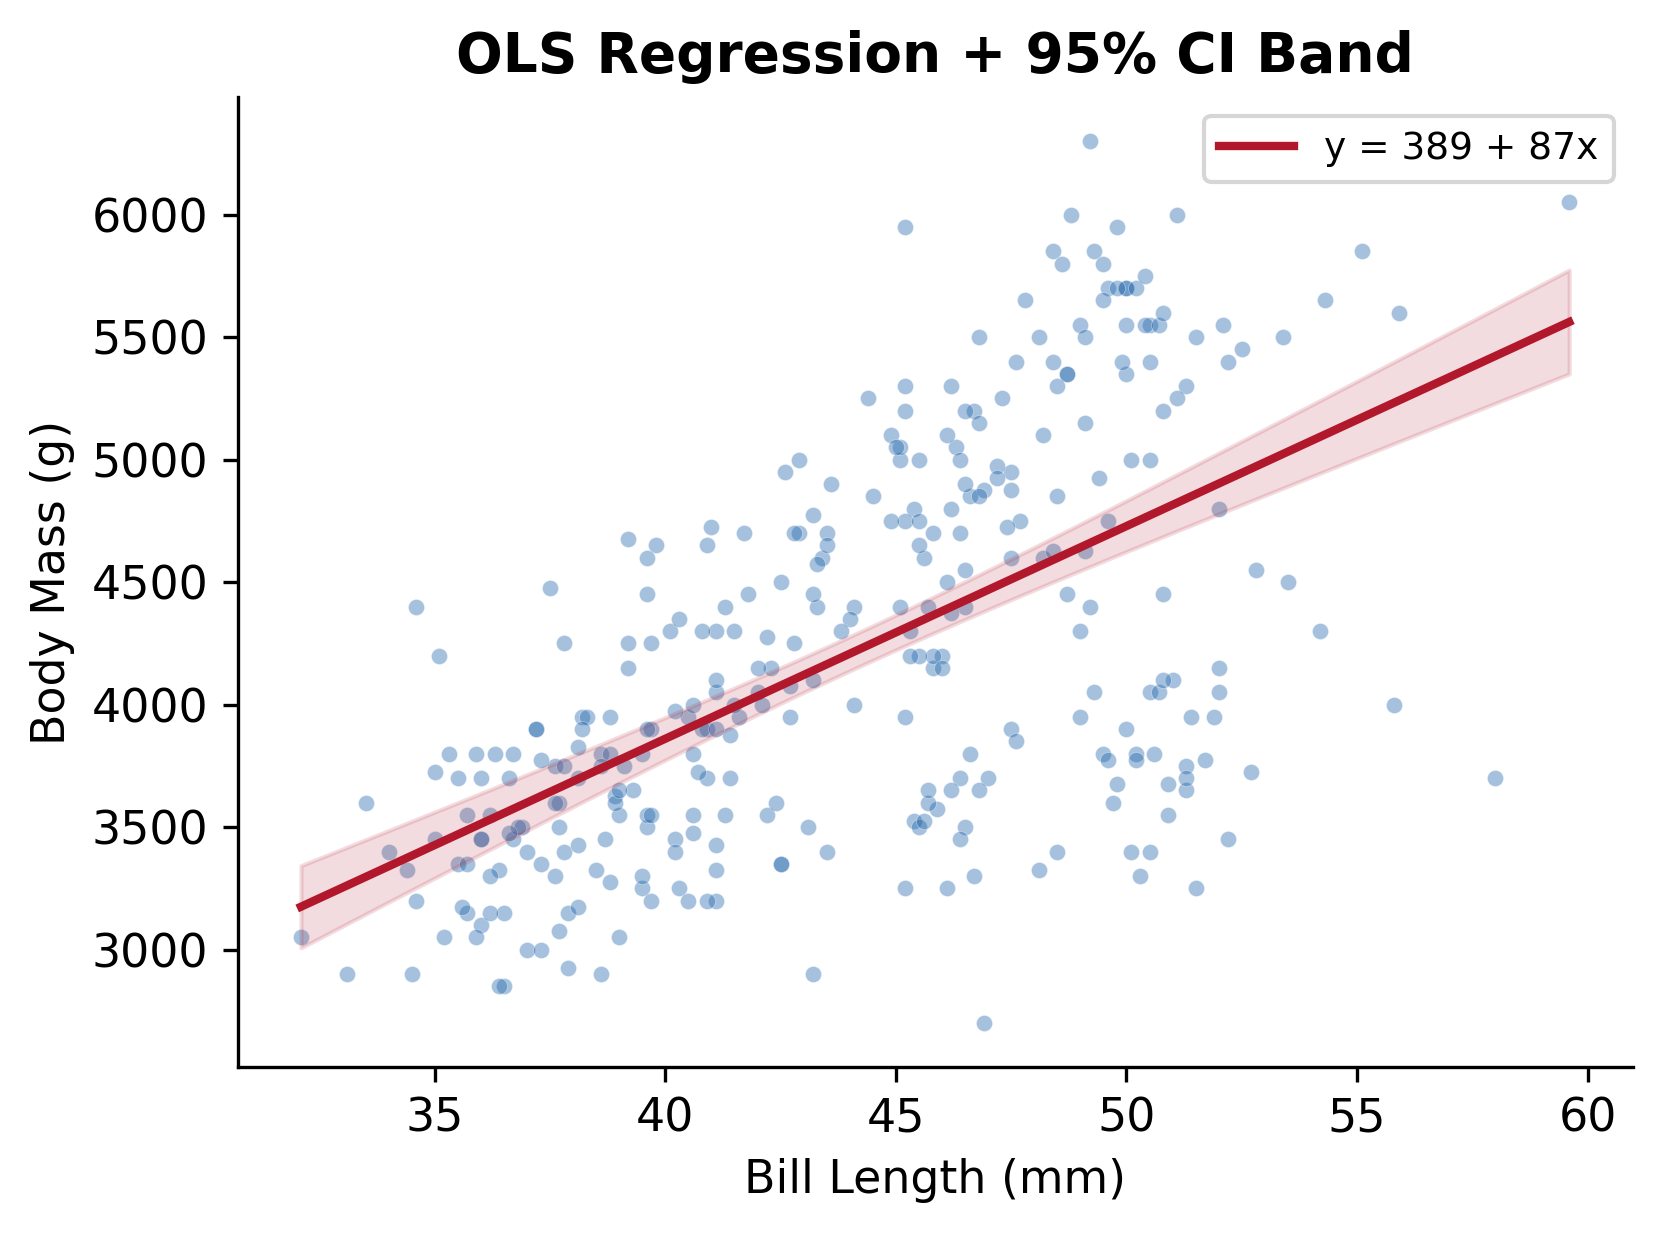
\includegraphics[width=\textwidth]{m2_3_regression_ci.png}
\begin{exampleblock}{Data Insight}
    \scriptsize \texttt{sns.regplot(ci=95)} bootstraps the CI band by default. \texttt{ci=None} removes it. \texttt{order=2} fits a quadratic.
\end{exampleblock}
\end{column}
\end{columns}
\end{frame}

% ── 66 ──
\begin{frame}{Confidence Interval vs.\ Prediction Interval}
\smark{66/300}
\centering
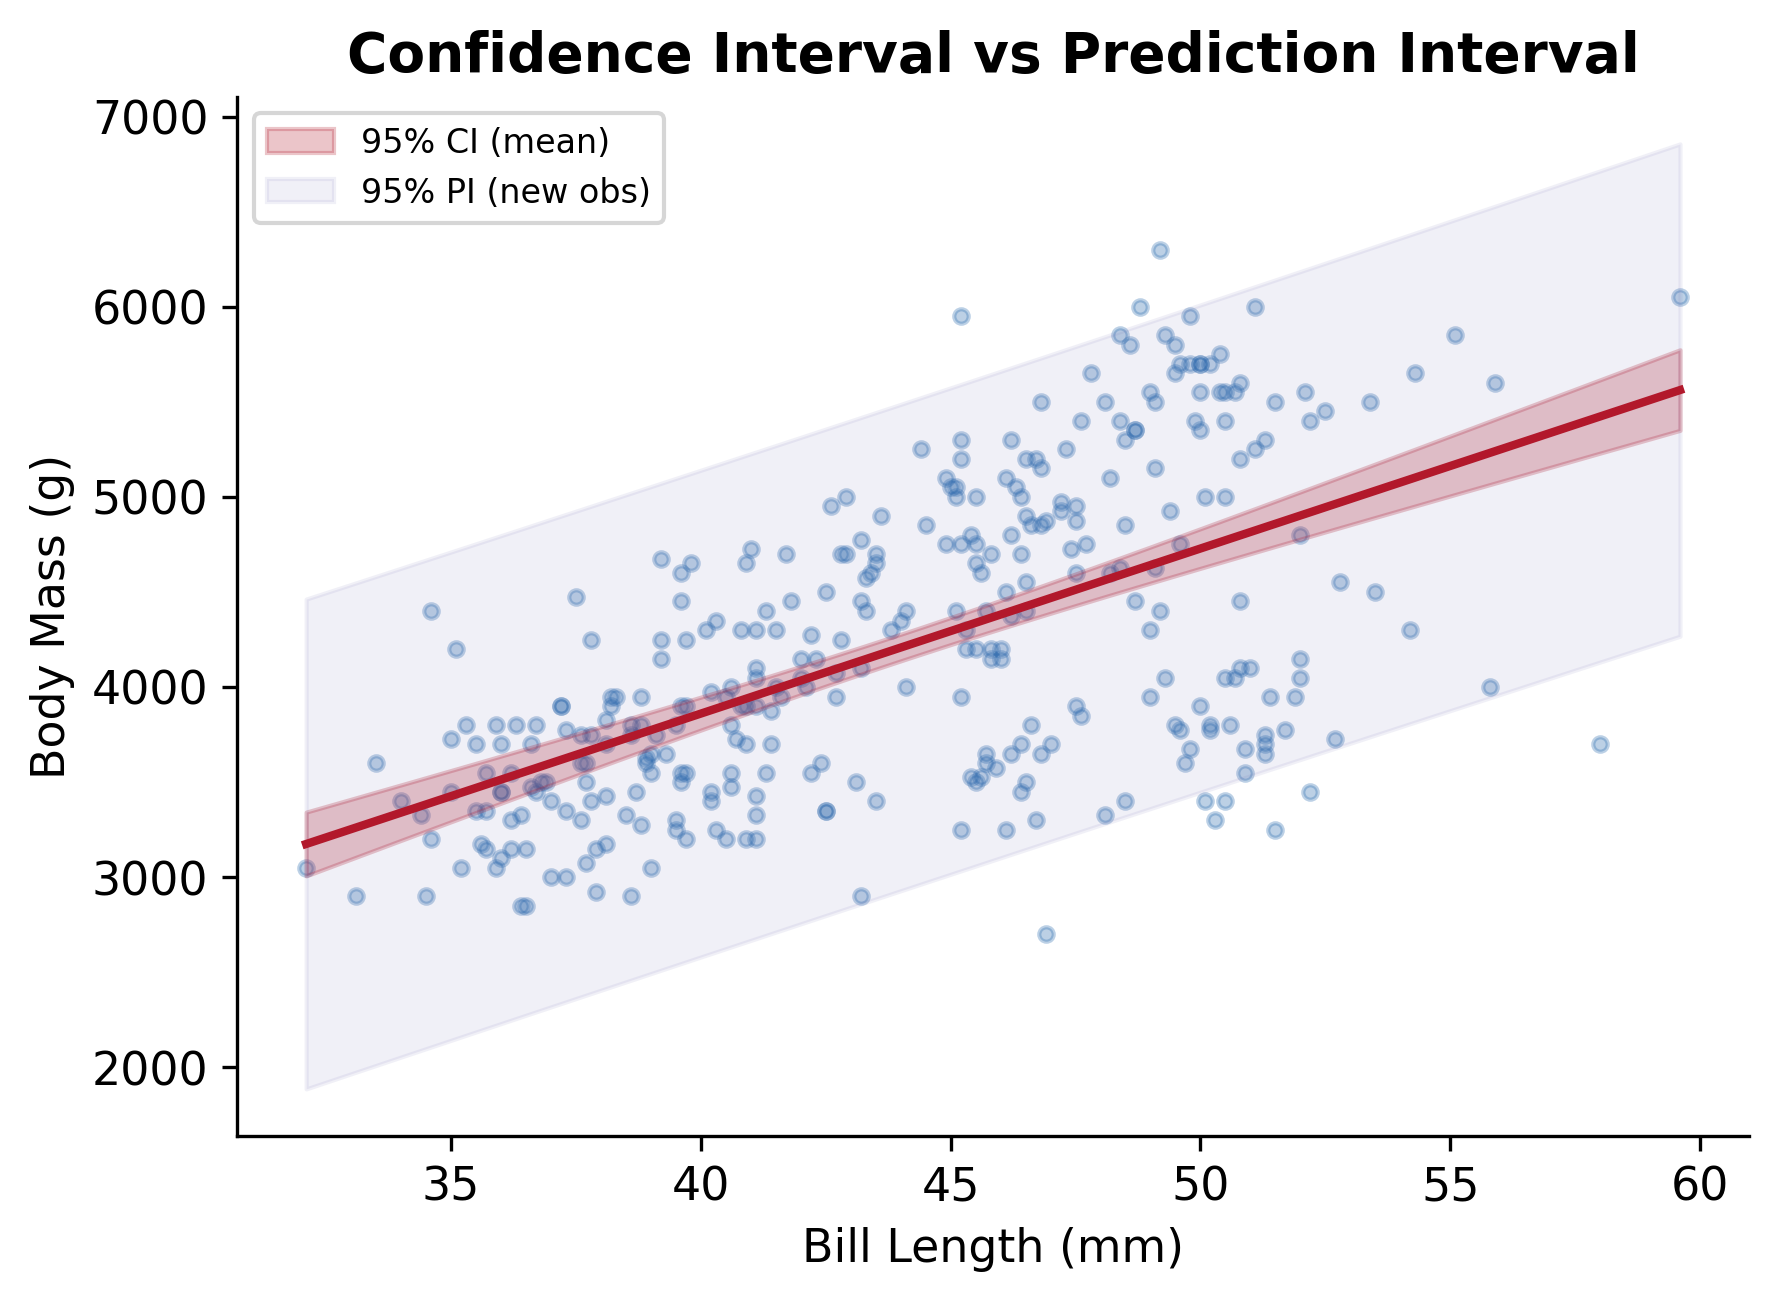
\includegraphics[width=0.68\textwidth]{m2_3_ci_vs_pi.png}

\vspace{0.2cm}
\begin{columns}[T]
\begin{column}{0.48\textwidth}
\begin{itemize}
    \item \textbf{CI} (narrow): where the true \textbf{mean} response lies
    \item \textbf{PI} (wide): where a \textbf{new individual} observation will fall
    \item PI $>$ CI because it adds individual-level variance ($\sigma^2$)
\end{itemize}
\end{column}
\begin{column}{0.48\textwidth}
\begin{alertblock}{Pro-Tip}
    \scriptsize \texttt{geom\_smooth()} shows only the CI. For PIs, use \texttt{predict(model, interval="prediction")} in R or \texttt{get\_prediction()} from \texttt{statsmodels} in Python, then plot manually.
\end{alertblock}
\end{column}
\end{columns}
\end{frame}

% ── 67 ──
\begin{frame}[fragile]{CI vs.\ PI --- Code}\smark{67/300}
\begin{columns}[T]
\begin{column}{0.48\textwidth}
\begin{lstlisting}[style=Rstyle]
model <- lm(body_mass_g ~
  bill_length_mm, data=penguins)

pred <- predict(model,
  interval = "confidence")
pi   <- predict(model,
  interval = "prediction")

df <- cbind(penguins, pred, pi)

ggplot(df, aes(bill_length_mm)) +
  geom_point(aes(y=body_mass_g),
    alpha=0.3) +
  geom_line(aes(y=fit),
    color="#B2182B") +
  geom_ribbon(aes(ymin=lwr,
    ymax=upr), alpha=0.2,
    fill="#B2182B") +   # CI
  geom_ribbon(aes(ymin=lwr.1,
    ymax=upr.1), alpha=0.1,
    fill="#7570B3")     # PI
\end{lstlisting}
\end{column}
\begin{column}{0.48\textwidth}
\begin{lstlisting}[style=Pystyle]
import statsmodels.api as sm

X = sm.add_constant(
    penguins["bill_length_mm"])
model = sm.OLS(
    penguins["body_mass_g"],
    X).fit()

pred = model.get_prediction(X)
ci = pred.conf_int(alpha=0.05)
pi = pred.conf_int(
    obs=True, alpha=0.05)

ax.fill_between(x_sorted,
    ci_lo, ci_hi, alpha=0.2,
    color="#B2182B", label="CI")
ax.fill_between(x_sorted,
    pi_lo, pi_hi, alpha=0.1,
    color="#7570B3", label="PI")
\end{lstlisting}
\end{column}
\end{columns}
\end{frame}

% ── 68 ──
\begin{frame}{The Classic 4-Panel Diagnostic}
\smark{68/300}
\centering
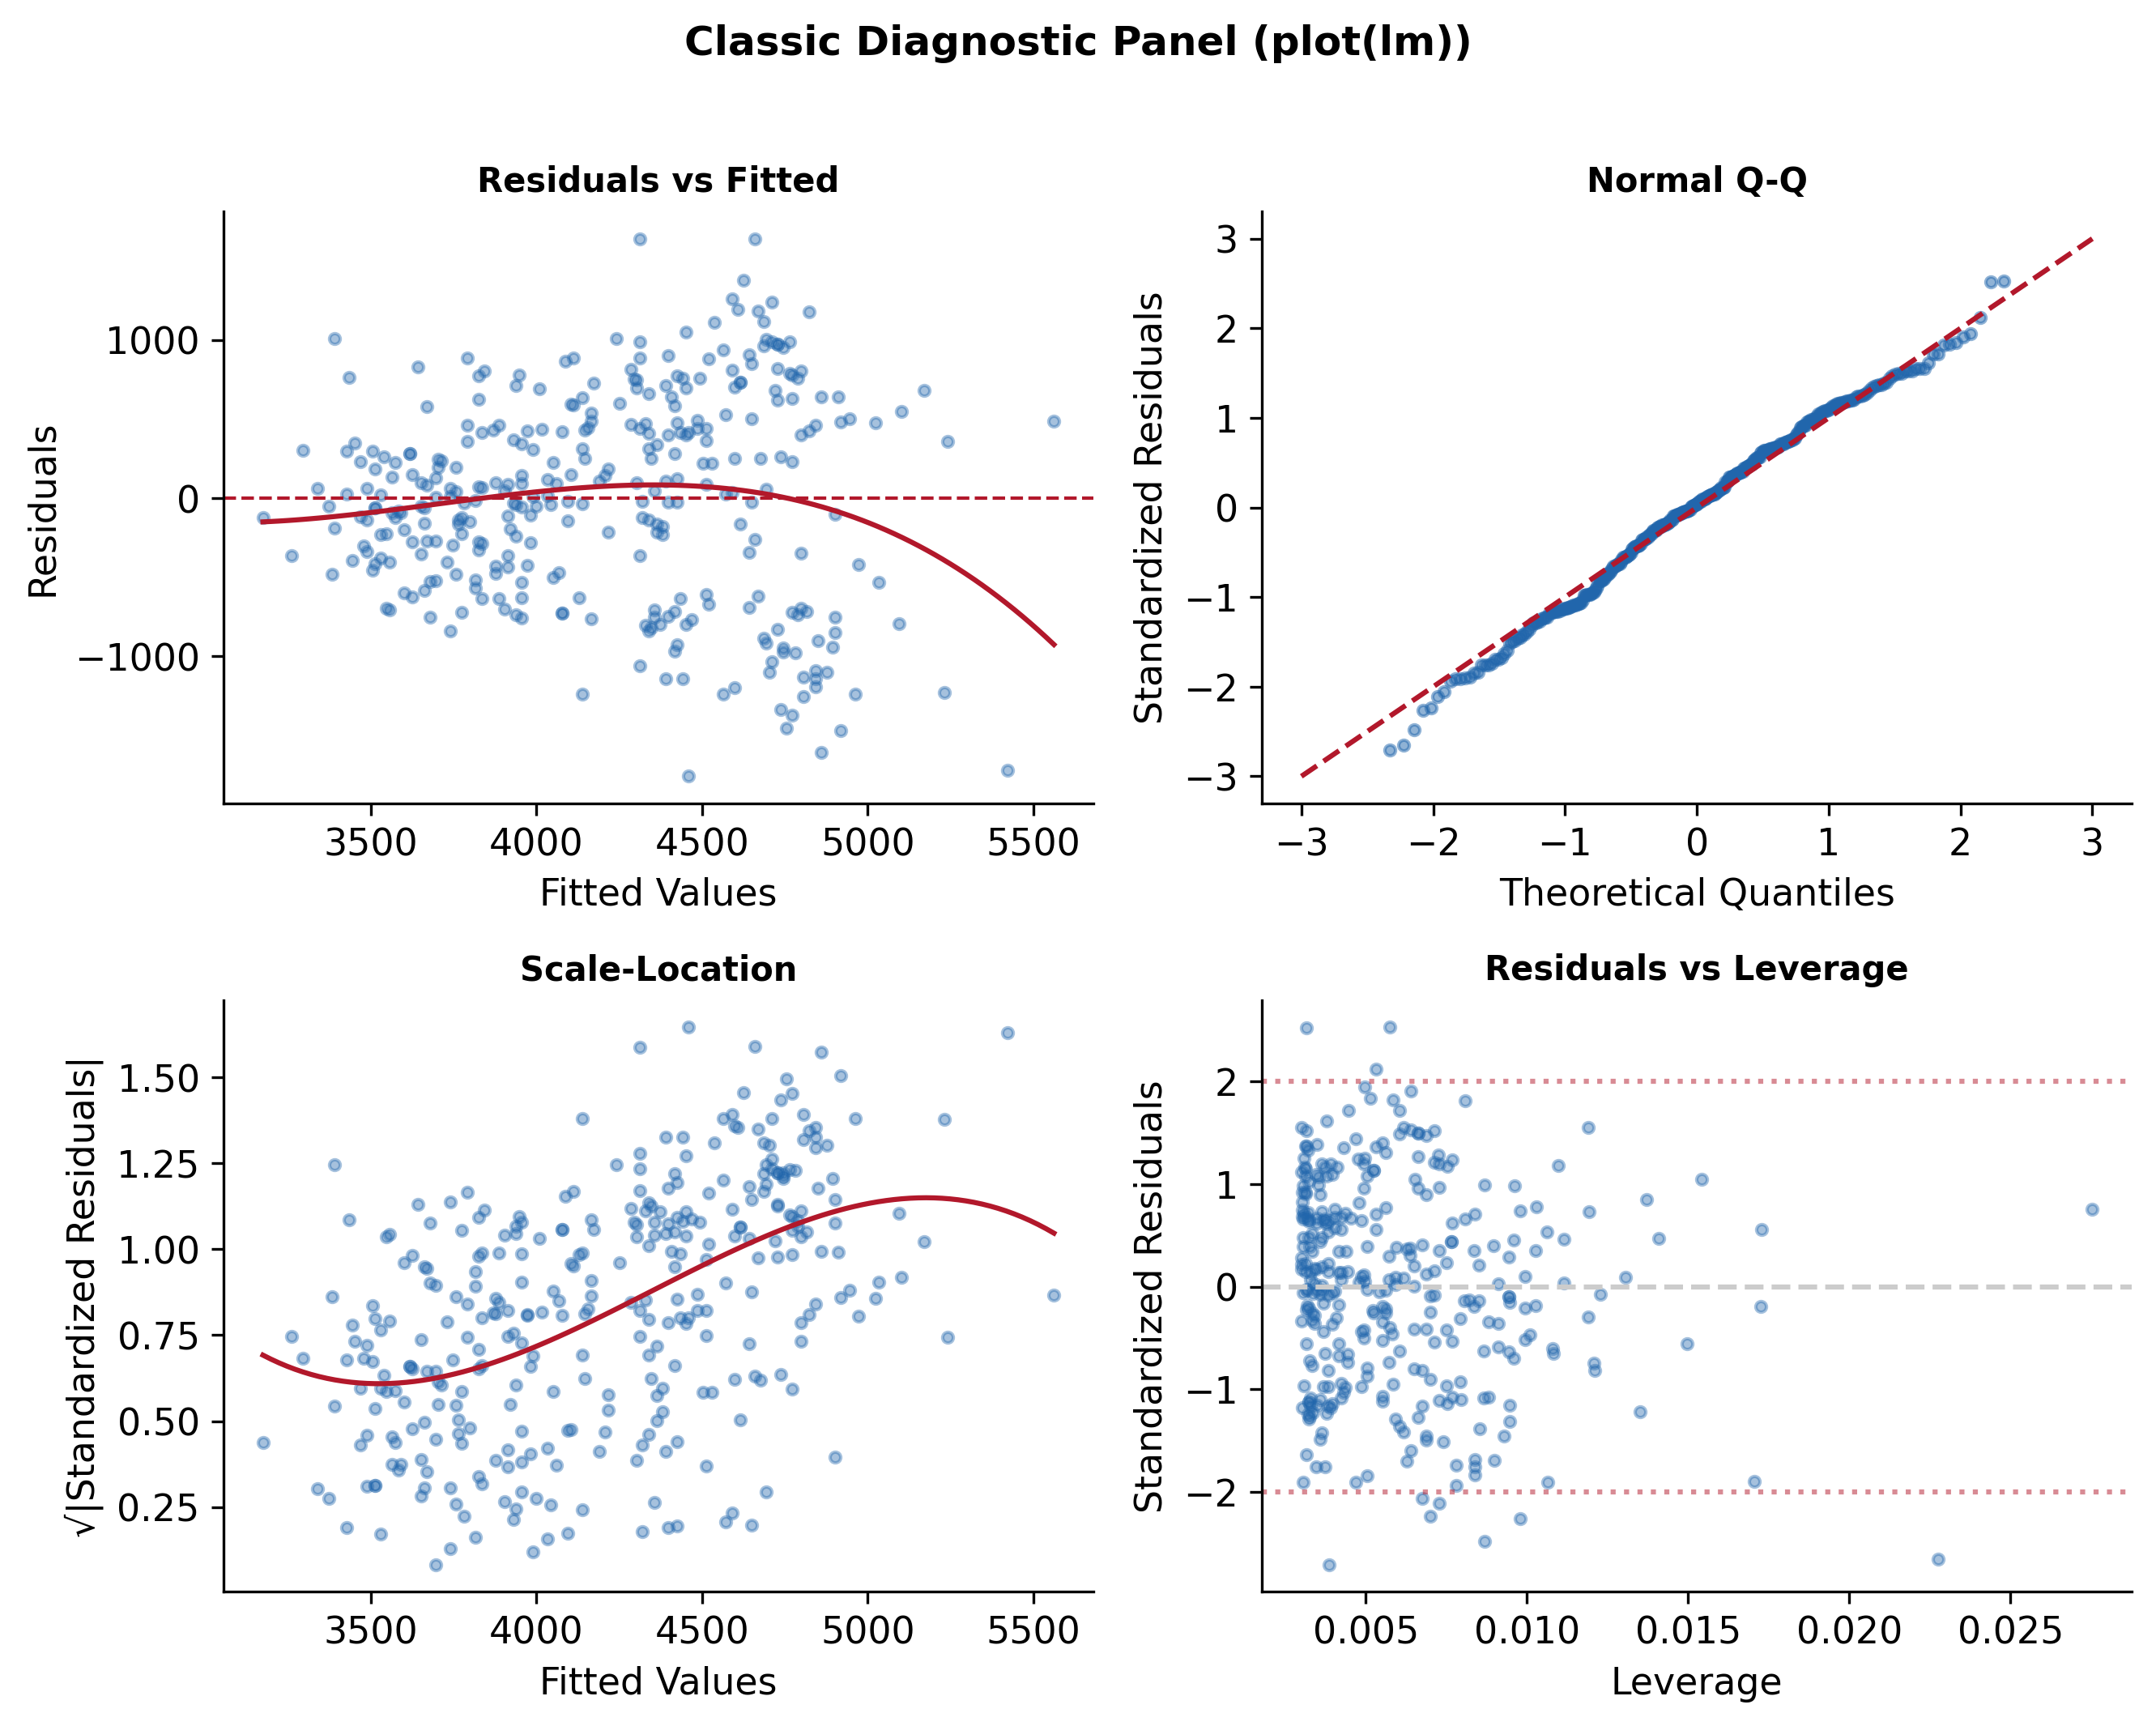
\includegraphics[width=0.78\textwidth]{m2_3_diagnostics_4panel.png}

\vspace{0.2cm}
\begin{exampleblock}{Data Insight}
    \scriptsize R's \texttt{plot(lm\_model)} produces these four panels automatically. Each diagnoses a different OLS assumption: linearity, normality, homoscedasticity, and influence.
\end{exampleblock}
\end{frame}

% ── 69 ──
\begin{frame}{Reading the 4 Panels}
\smark{69/300}
\centering\small
\begin{tabular}{@{}llll@{}}
    \toprule
    \textbf{Panel} & \textbf{Checks} & \textbf{Good Pattern} & \textbf{Bad Pattern} \\
    \midrule
    Resid vs.\ Fitted & Linearity      & Random scatter   & Curve (non-linearity) \\
    Normal Q-Q         & Normality      & Points on line   & S-curve (skew/tails) \\
    Scale-Location     & Homoscedasticity & Flat trend     & Fan/funnel shape \\
    Resid vs.\ Leverage& Influence      & No Cook's $>$1   & Extreme leverage + residual \\
    \bottomrule
\end{tabular}

\vspace{0.3cm}
\begin{alertblock}{Pro-Tip}
    \scriptsize Read them in order: (1) linearity is the most critical assumption. If the residual-vs-fitted plot shows curvature, fix the model specification before checking anything else.
\end{alertblock}
\end{frame}

% ── 70 ──
\begin{frame}[fragile]{4-Panel Diagnostics --- \Rlang}\smark{70/300}
\begin{columns}[T]
\begin{column}{0.55\textwidth}
\begin{lstlisting}[style=Rstyle]
model <- lm(body_mass_g ~
  bill_length_mm, data=penguins)

# Base R (instant)
par(mfrow = c(2, 2))
plot(model)

# ggplot2 (via performance pkg)
library(performance)
check_model(model)
# Produces 6+ panels with
# interpretation guidelines

# Or individual panels:
library(ggfortify)
autoplot(model)
\end{lstlisting}
\end{column}
\begin{column}{0.42\textwidth}
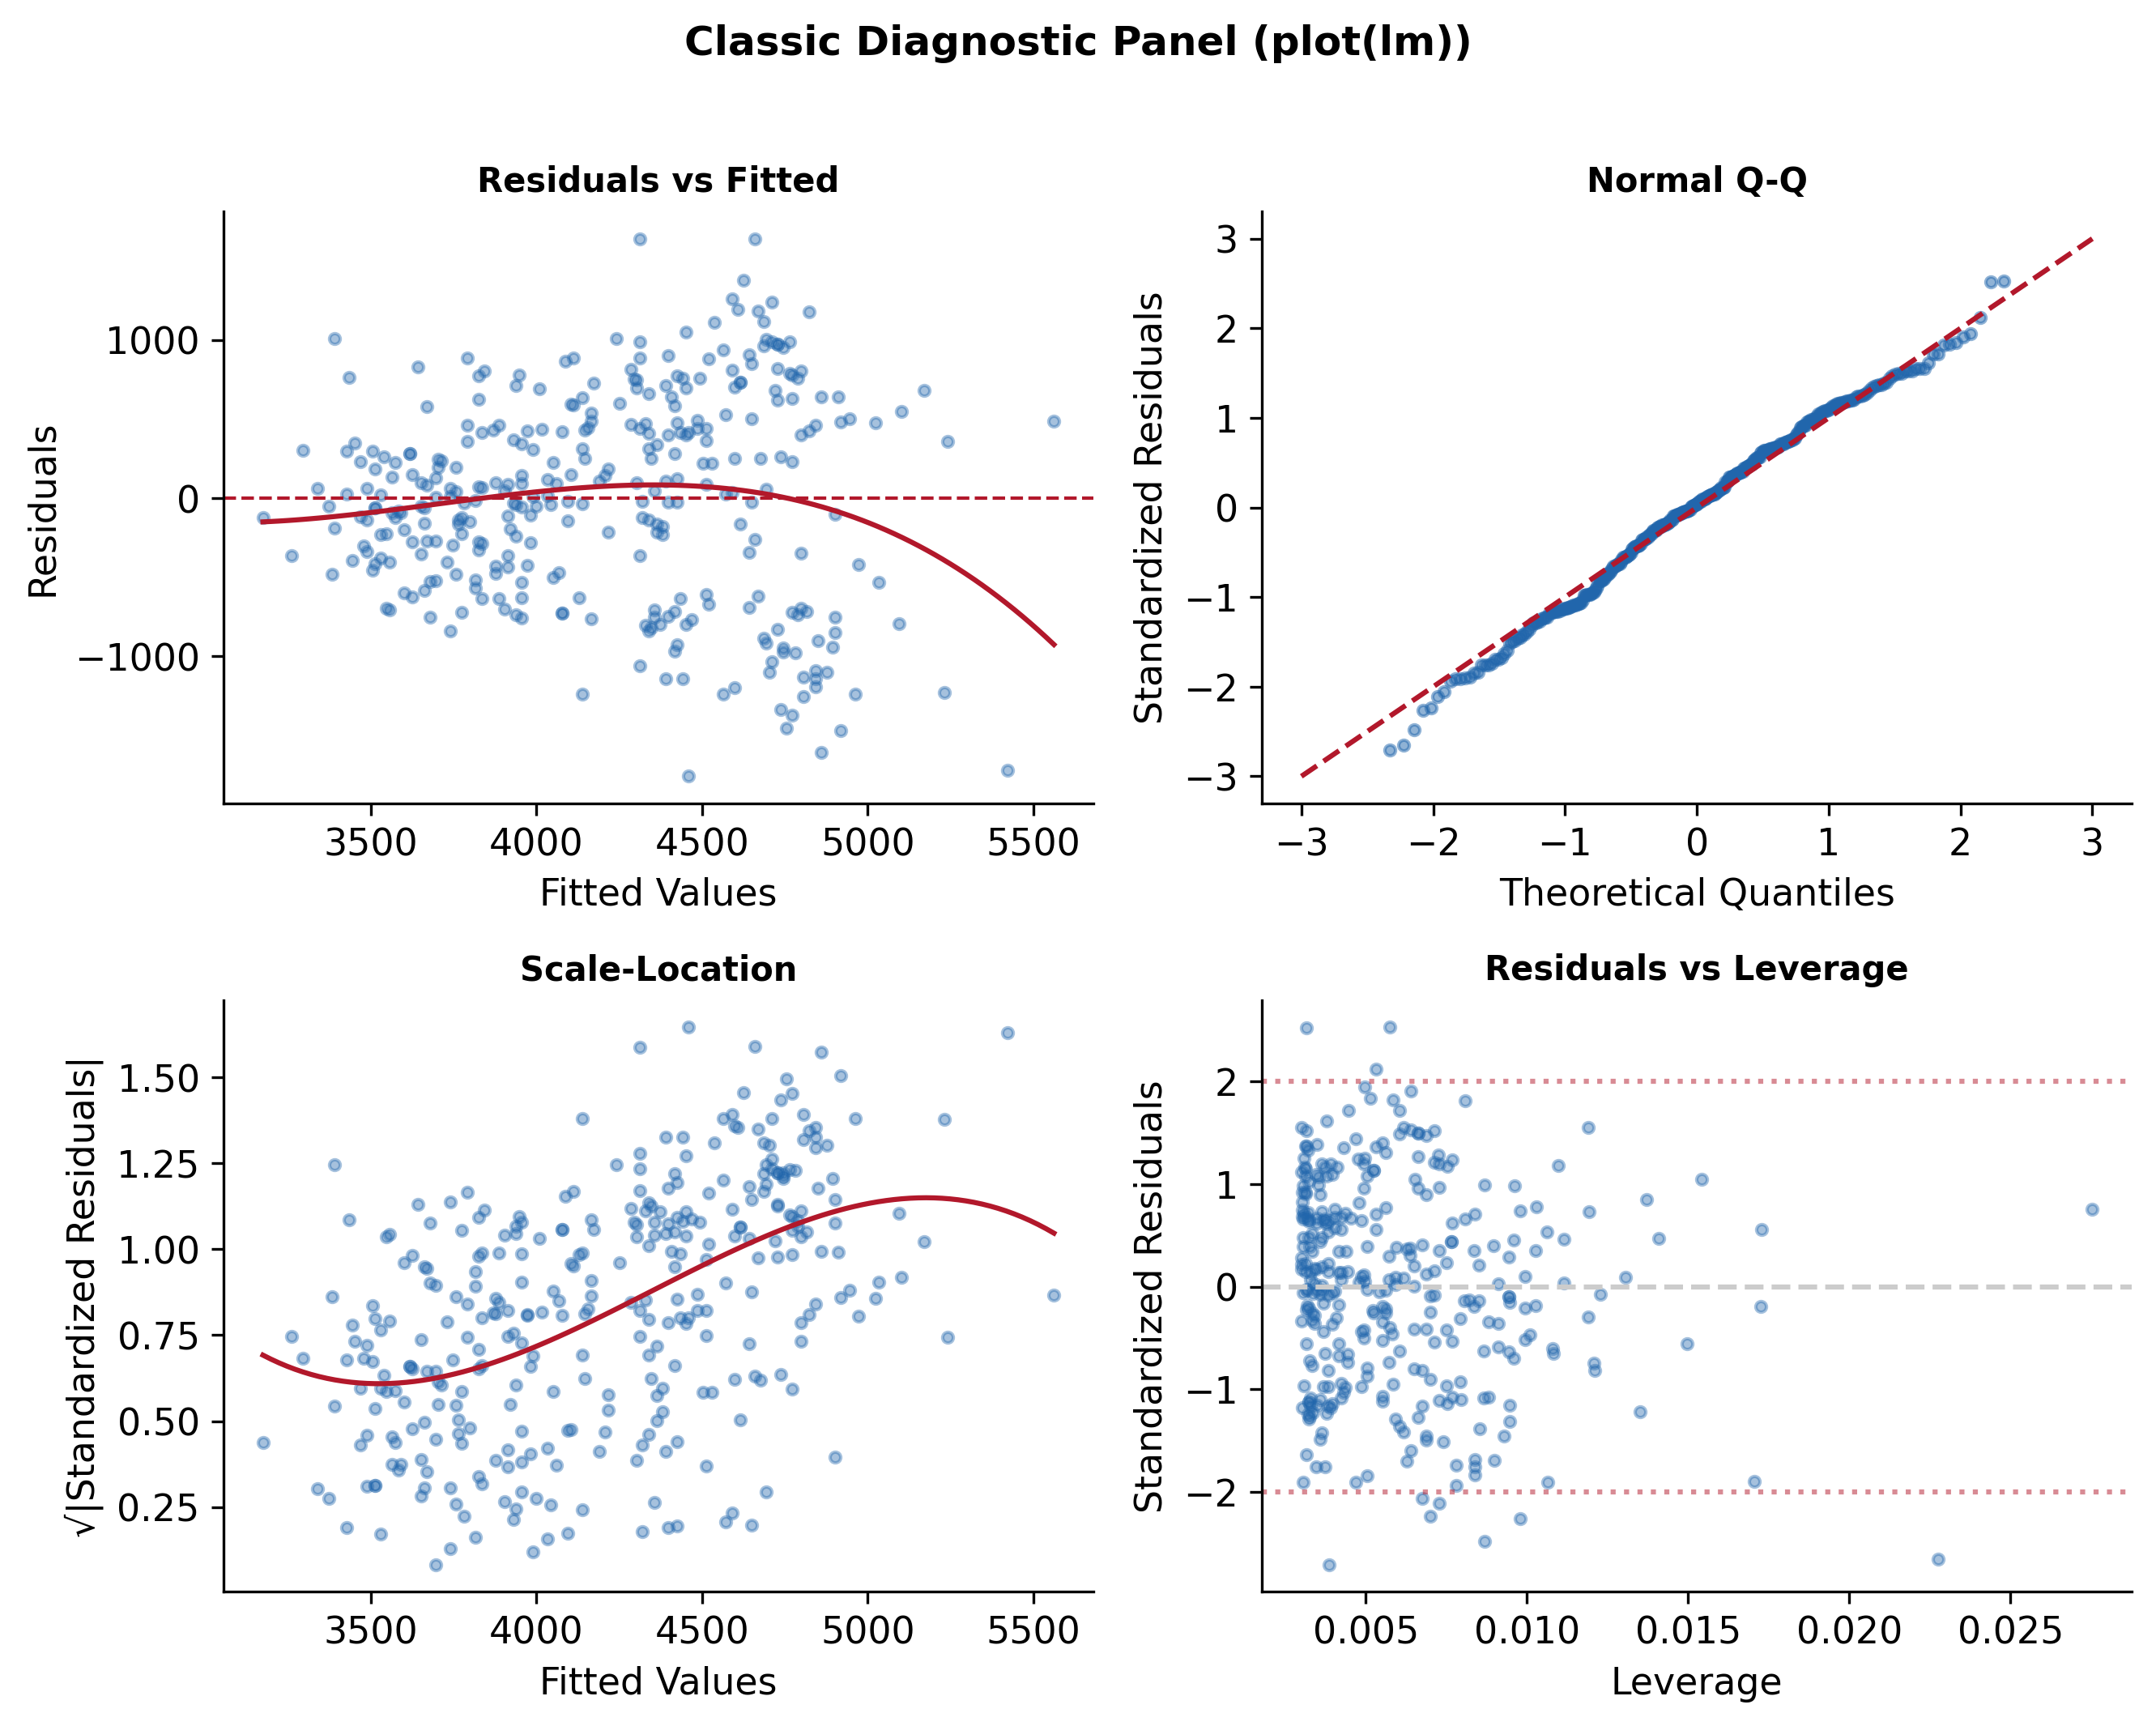
\includegraphics[width=\textwidth]{m2_3_diagnostics_4panel.png}
\begin{exampleblock}{Data Insight}
    \scriptsize \texttt{performance::check\_model()} is the modern R approach: beautiful ggplot2-based panels with interpretive annotations built in.
\end{exampleblock}
\end{column}
\end{columns}
\end{frame}

% ── 71 ──
\begin{frame}[fragile]{4-Panel Diagnostics --- \Python}\smark{71/300}
\begin{columns}[T]
\begin{column}{0.55\textwidth}
\begin{lstlisting}[style=Pystyle]
import statsmodels.api as sm

model = sm.OLS(y, X).fit()

# Built-in influence plot
fig = sm.graphics.plot_regress_exog(
    model, "bill_length_mm")

# Individual panels
fig, ax = plt.subplots()
sm.graphics.plot_fit(
    model, "bill_length_mm", ax=ax)

# Manual residual-vs-fitted
resid = model.resid
fitted = model.fittedvalues
ax.scatter(fitted, resid, s=10)
ax.axhline(0, color="#B2182B",
    linestyle="--")
\end{lstlisting}
\end{column}
\begin{column}{0.42\textwidth}
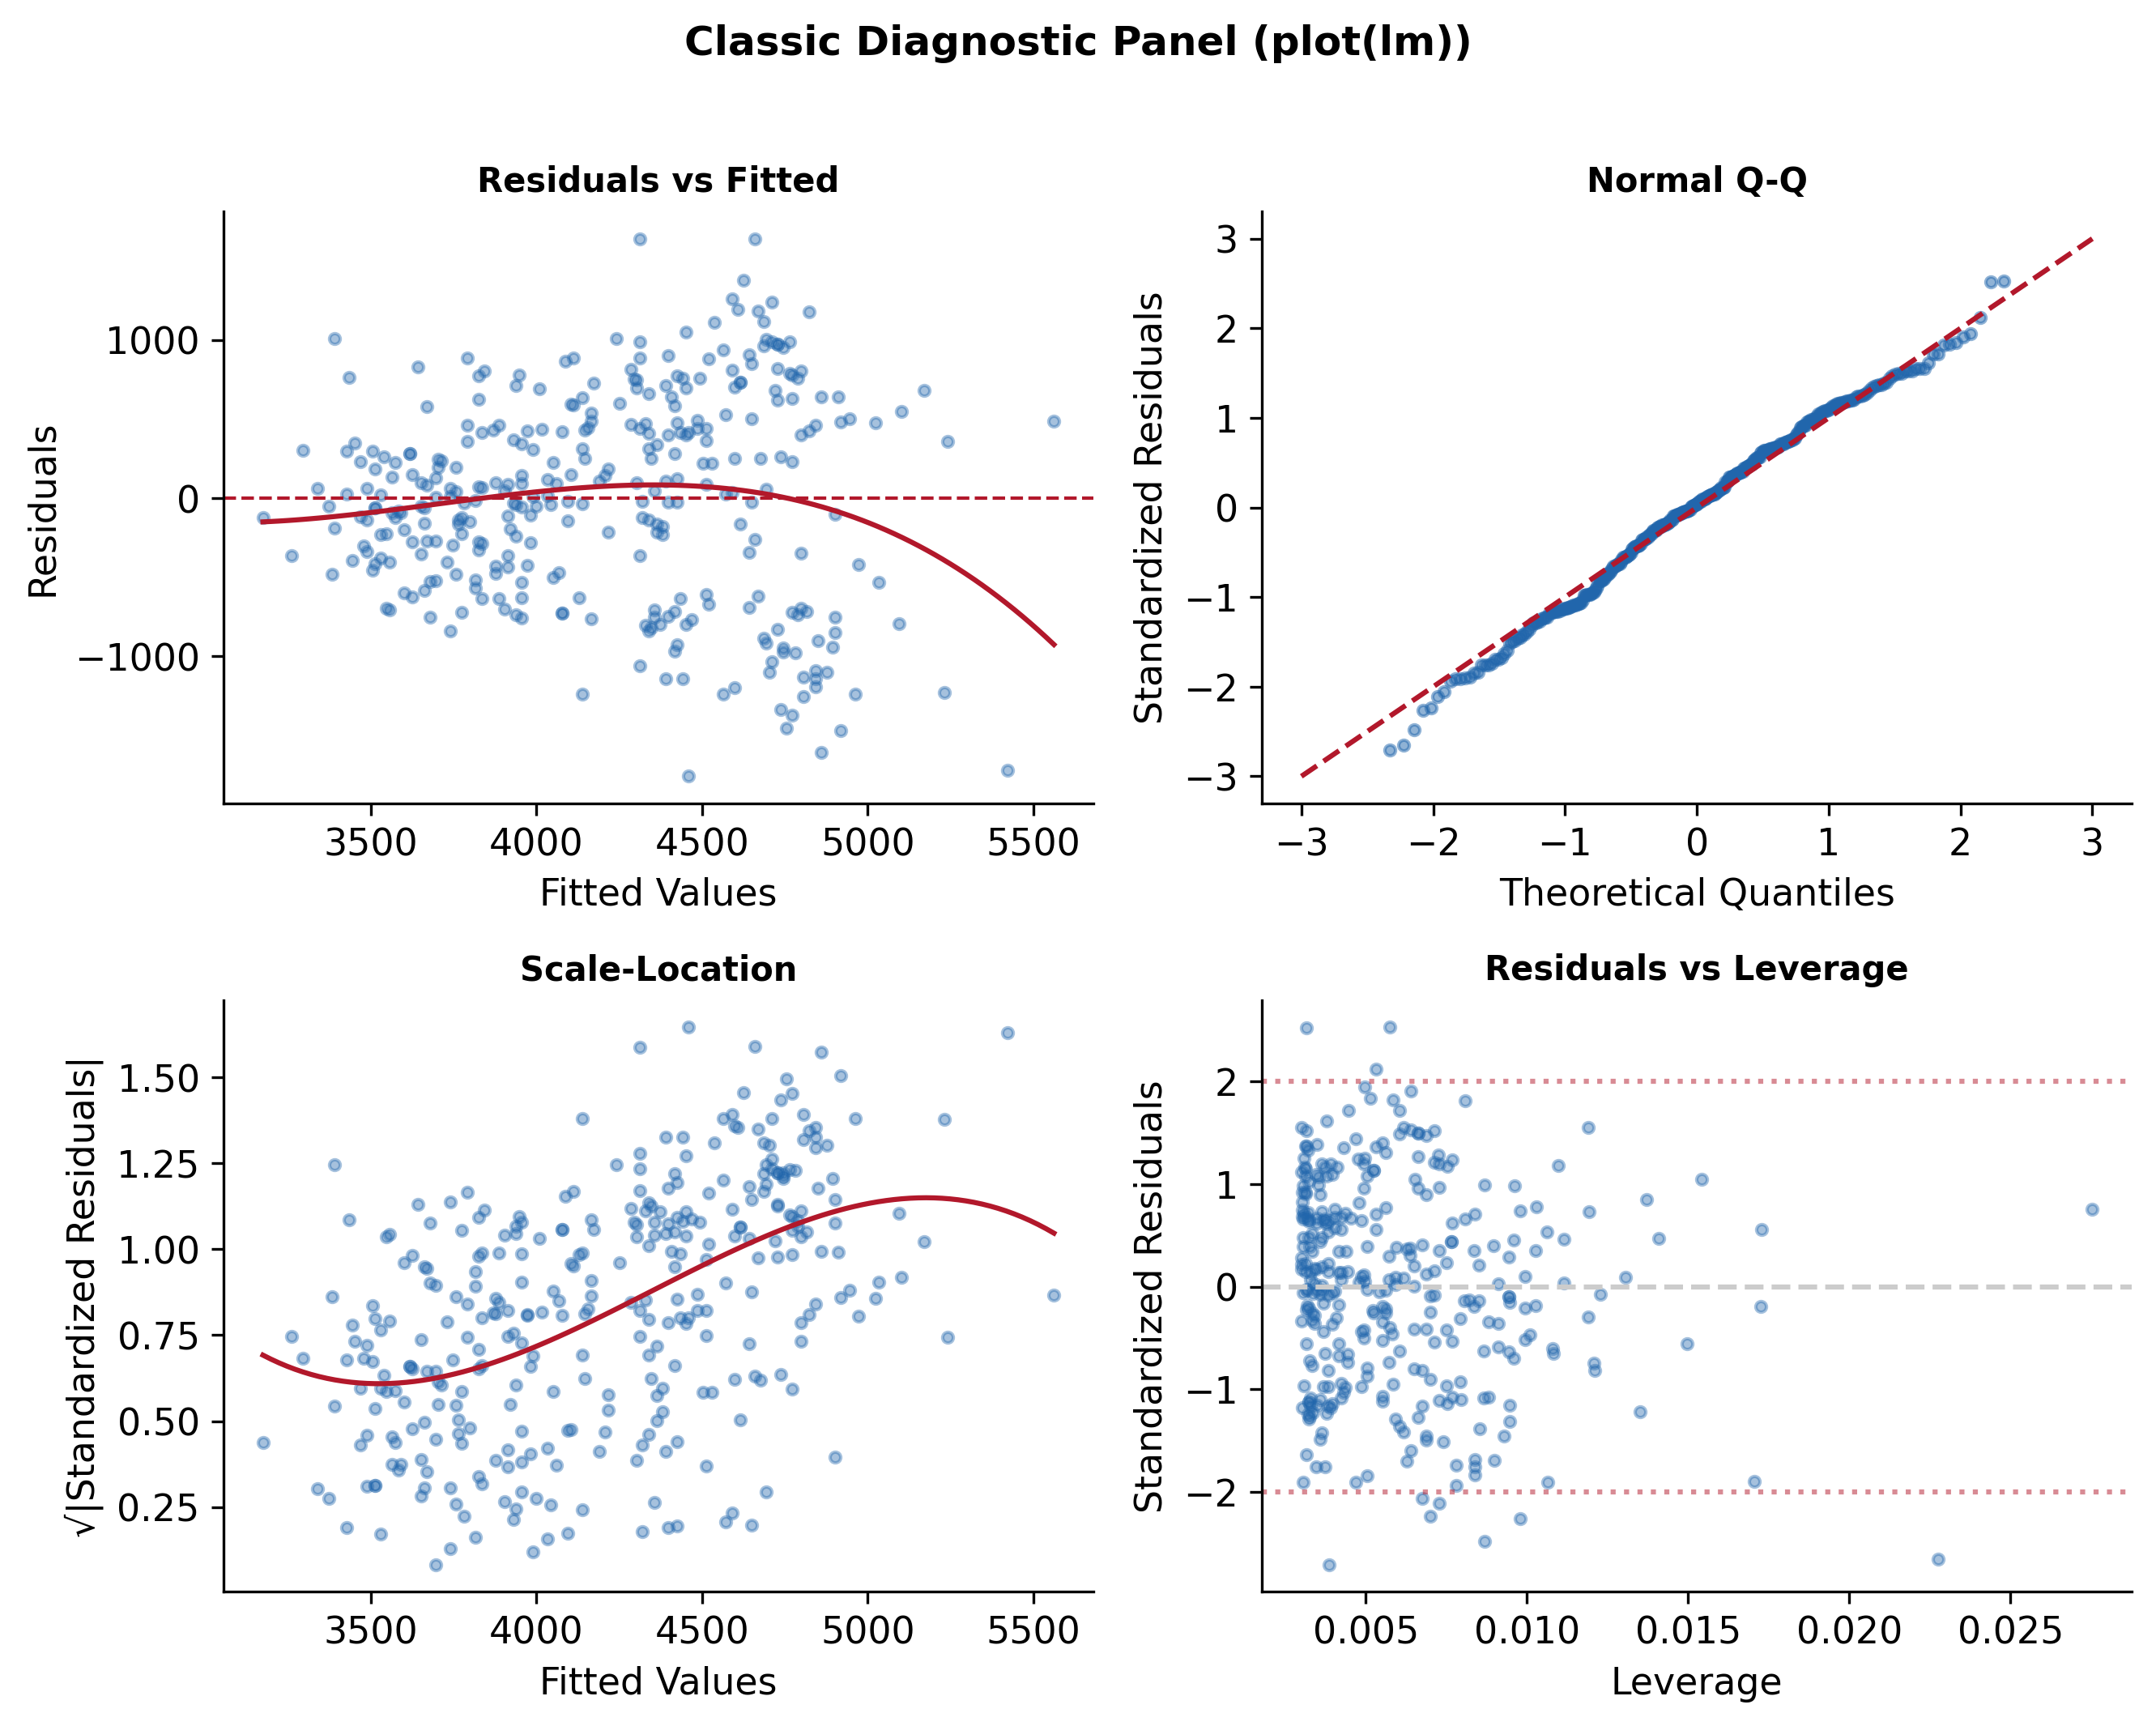
\includegraphics[width=\textwidth]{m2_3_diagnostics_4panel.png}
\begin{alertblock}{Pro-Tip}
    \scriptsize \texttt{statsmodels.graphics} provides several built-in diagnostic plots. For full control, extract \texttt{model.resid}, \texttt{model.fittedvalues}, and \texttt{model.get\_influence()} and plot manually.
\end{alertblock}
\end{column}
\end{columns}
\end{frame}

% ── 72 ──
\begin{frame}{Residuals vs.\ Fitted: Good and Bad}
\smark{72/300}
\centering
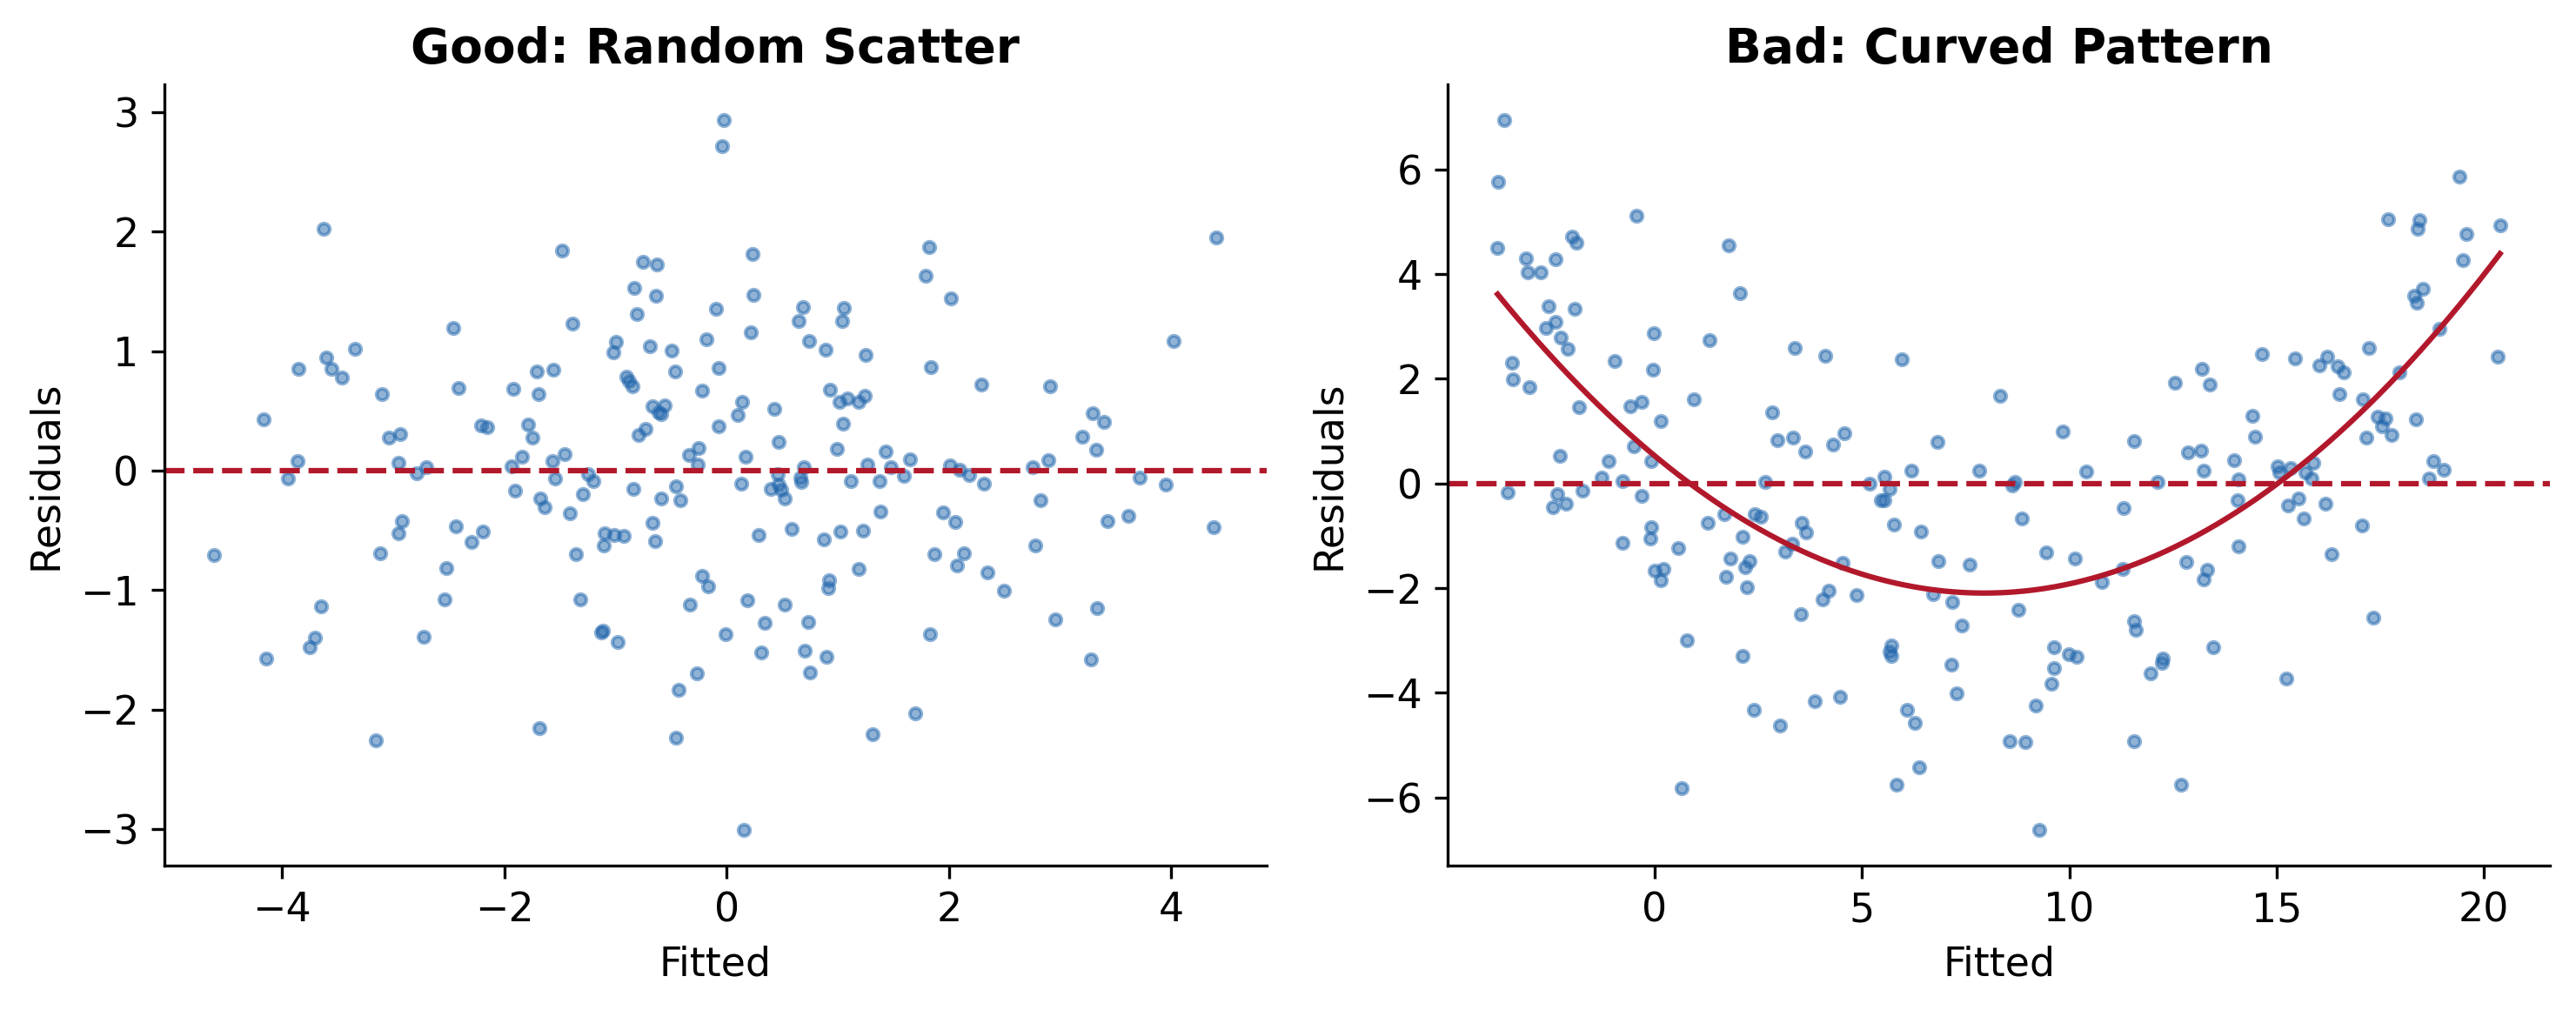
\includegraphics[width=0.88\textwidth]{m2_3_resid_good_bad.png}

\vspace{0.2cm}
\begin{columns}[T]
\begin{column}{0.48\textwidth}
\begin{exampleblock}{Data Insight}
    \scriptsize Left: residuals scatter randomly around zero with constant spread --- linearity and homoscedasticity satisfied. Right: a U-shaped curve means the linear model misses a quadratic relationship.
\end{exampleblock}
\end{column}
\begin{column}{0.48\textwidth}
\begin{alertblock}{Pro-Tip}
    \scriptsize Add a LOESS smoother (red line) to the residual plot to make non-linearity visible. In ggplot2: \texttt{geom\_smooth(method="loess")}. A flat line at 0 = good.
\end{alertblock}
\end{column}
\end{columns}
\end{frame}

% ── 73 ──
\begin{frame}{Heteroscedasticity: The Funnel Shape}
\smark{73/300}
\centering
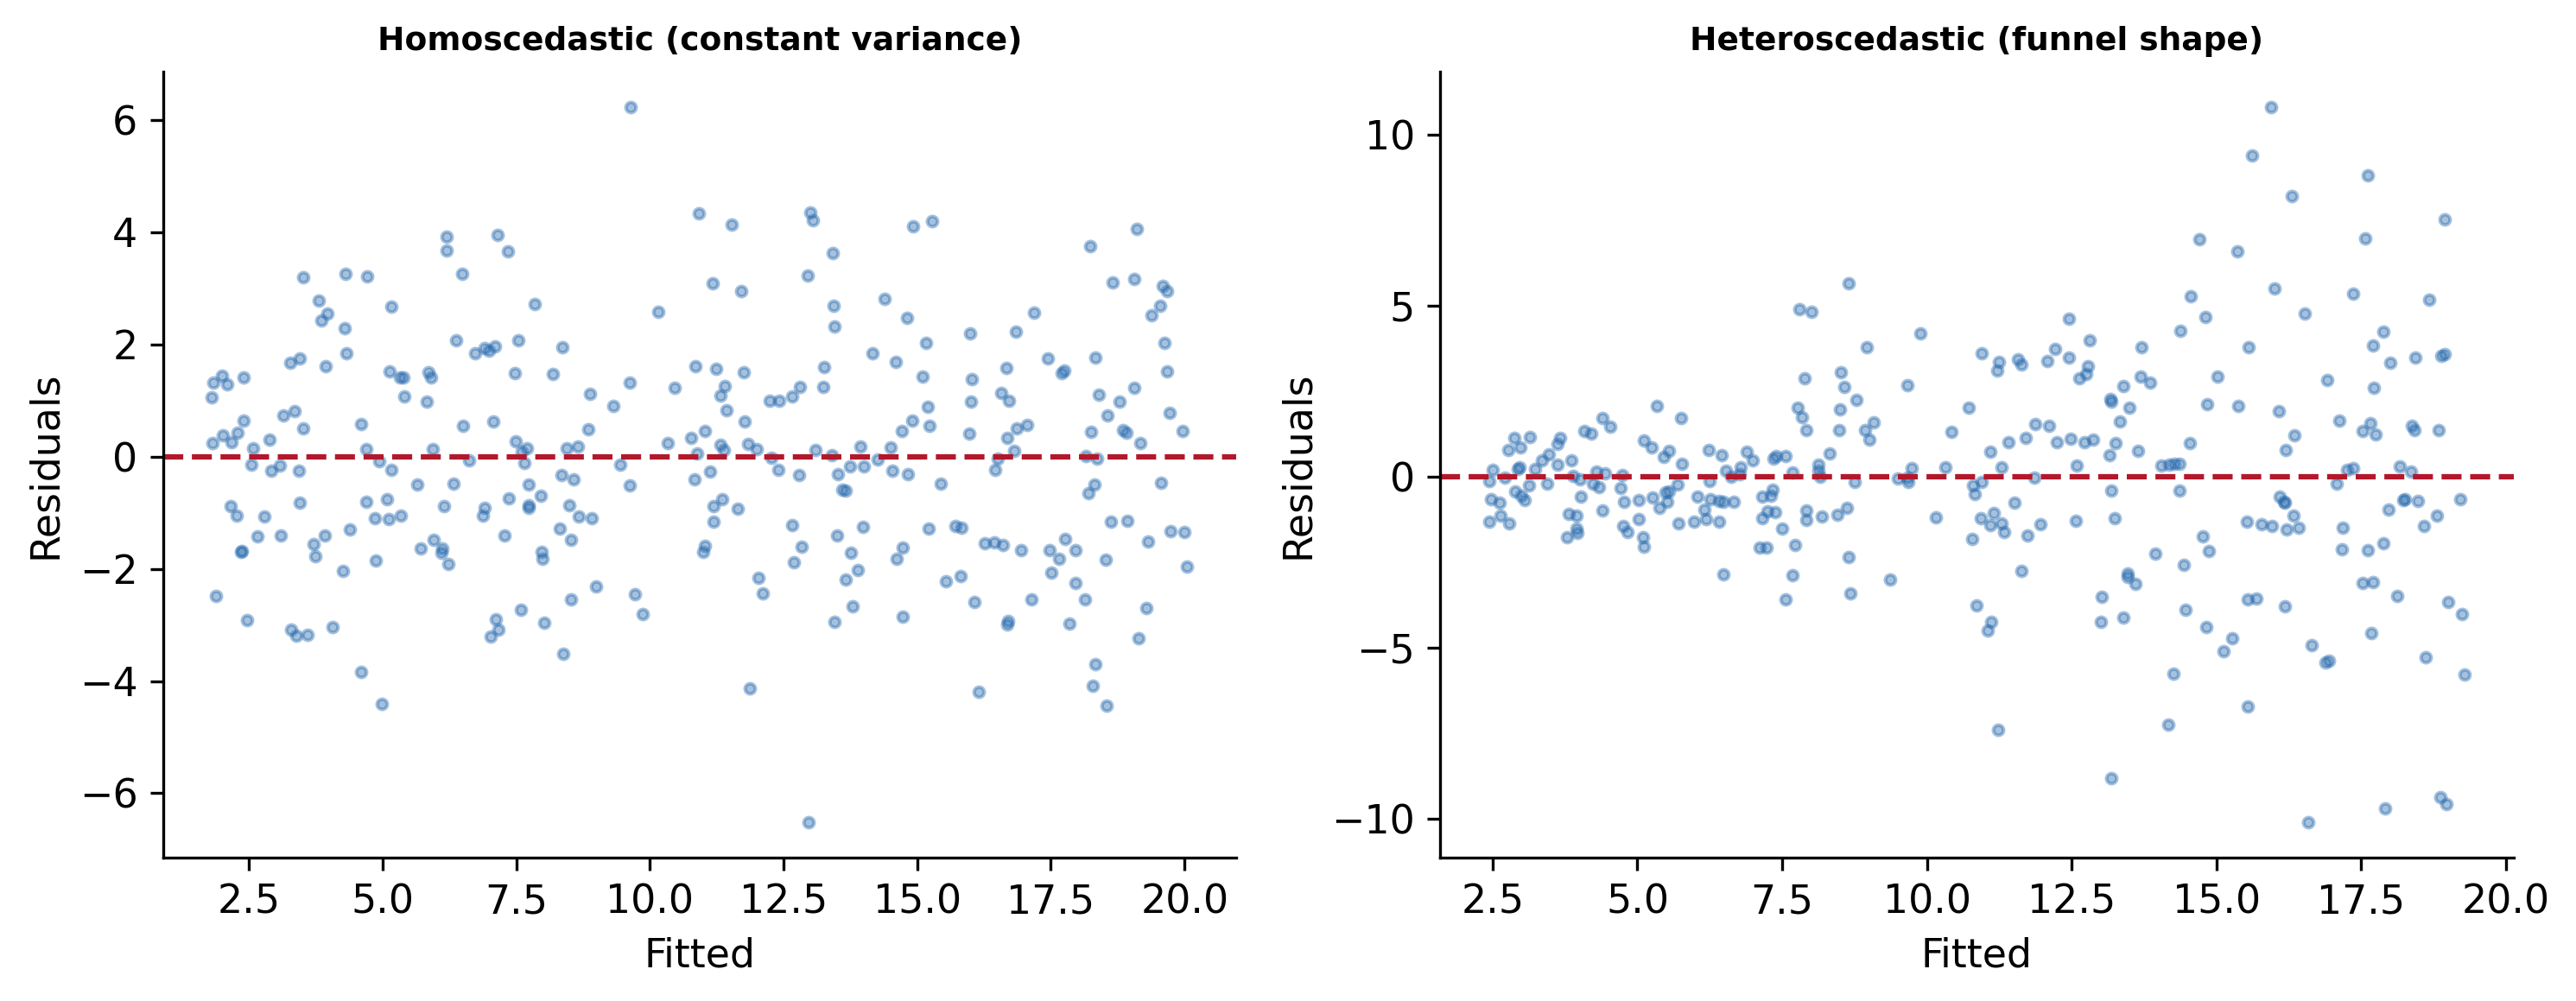
\includegraphics[width=0.88\textwidth]{m2_3_heteroscedasticity.png}

\vspace{0.2cm}
\begin{columns}[T]
\begin{column}{0.48\textwidth}
\begin{itemize}
    \item \textbf{Constant variance} (left): residual spread is uniform across fitted values
    \item \textbf{Funnel} (right): spread increases with fitted values
    \item Violates OLS assumption $\to$ biased standard errors
\end{itemize}
\end{column}
\begin{column}{0.48\textwidth}
\begin{alertblock}{Pro-Tip}
    \scriptsize Fixes for heteroscedasticity: (1) log-transform $y$; (2) weighted least squares; (3) robust standard errors (\texttt{sandwich::vcovHC()} in R, \texttt{model.get\_robustcov\_results()} in Python).
\end{alertblock}
\end{column}
\end{columns}
\end{frame}

% ── 74 ──
\begin{frame}[fragile]{Detecting Heteroscedasticity --- Code}\smark{74/300}
\begin{columns}[T]
\begin{column}{0.48\textwidth}
\begin{lstlisting}[style=Rstyle]
# Visual: Scale-Location plot
model <- lm(y ~ x, data=df)
plot(model, which = 3)

# Formal test: Breusch-Pagan
library(lmtest)
bptest(model)
# p < 0.05 = heteroscedastic

# Fix: robust SEs
library(sandwich)
coeftest(model,
  vcov = vcovHC(model, "HC1"))
\end{lstlisting}
\end{column}
\begin{column}{0.48\textwidth}
\begin{lstlisting}[style=Pystyle]
# Visual
fig, ax = plt.subplots()
ax.scatter(model.fittedvalues,
    np.sqrt(np.abs(
      model.resid / model.resid.std()
    )), s=10)

# Formal: Breusch-Pagan
from statsmodels.stats \
    .diagnostic import het_breuschpagan
bp = het_breuschpagan(
    model.resid, model.model.exog)
print(f"p = {bp[1]:.4f}")

# Fix: robust SEs
model.get_robustcov_results("HC1")
\end{lstlisting}
\end{column}
\end{columns}
\end{frame}

% ── 75 ──
\begin{frame}{Cook's Distance: Influential Points}
\smark{75/300}
\centering
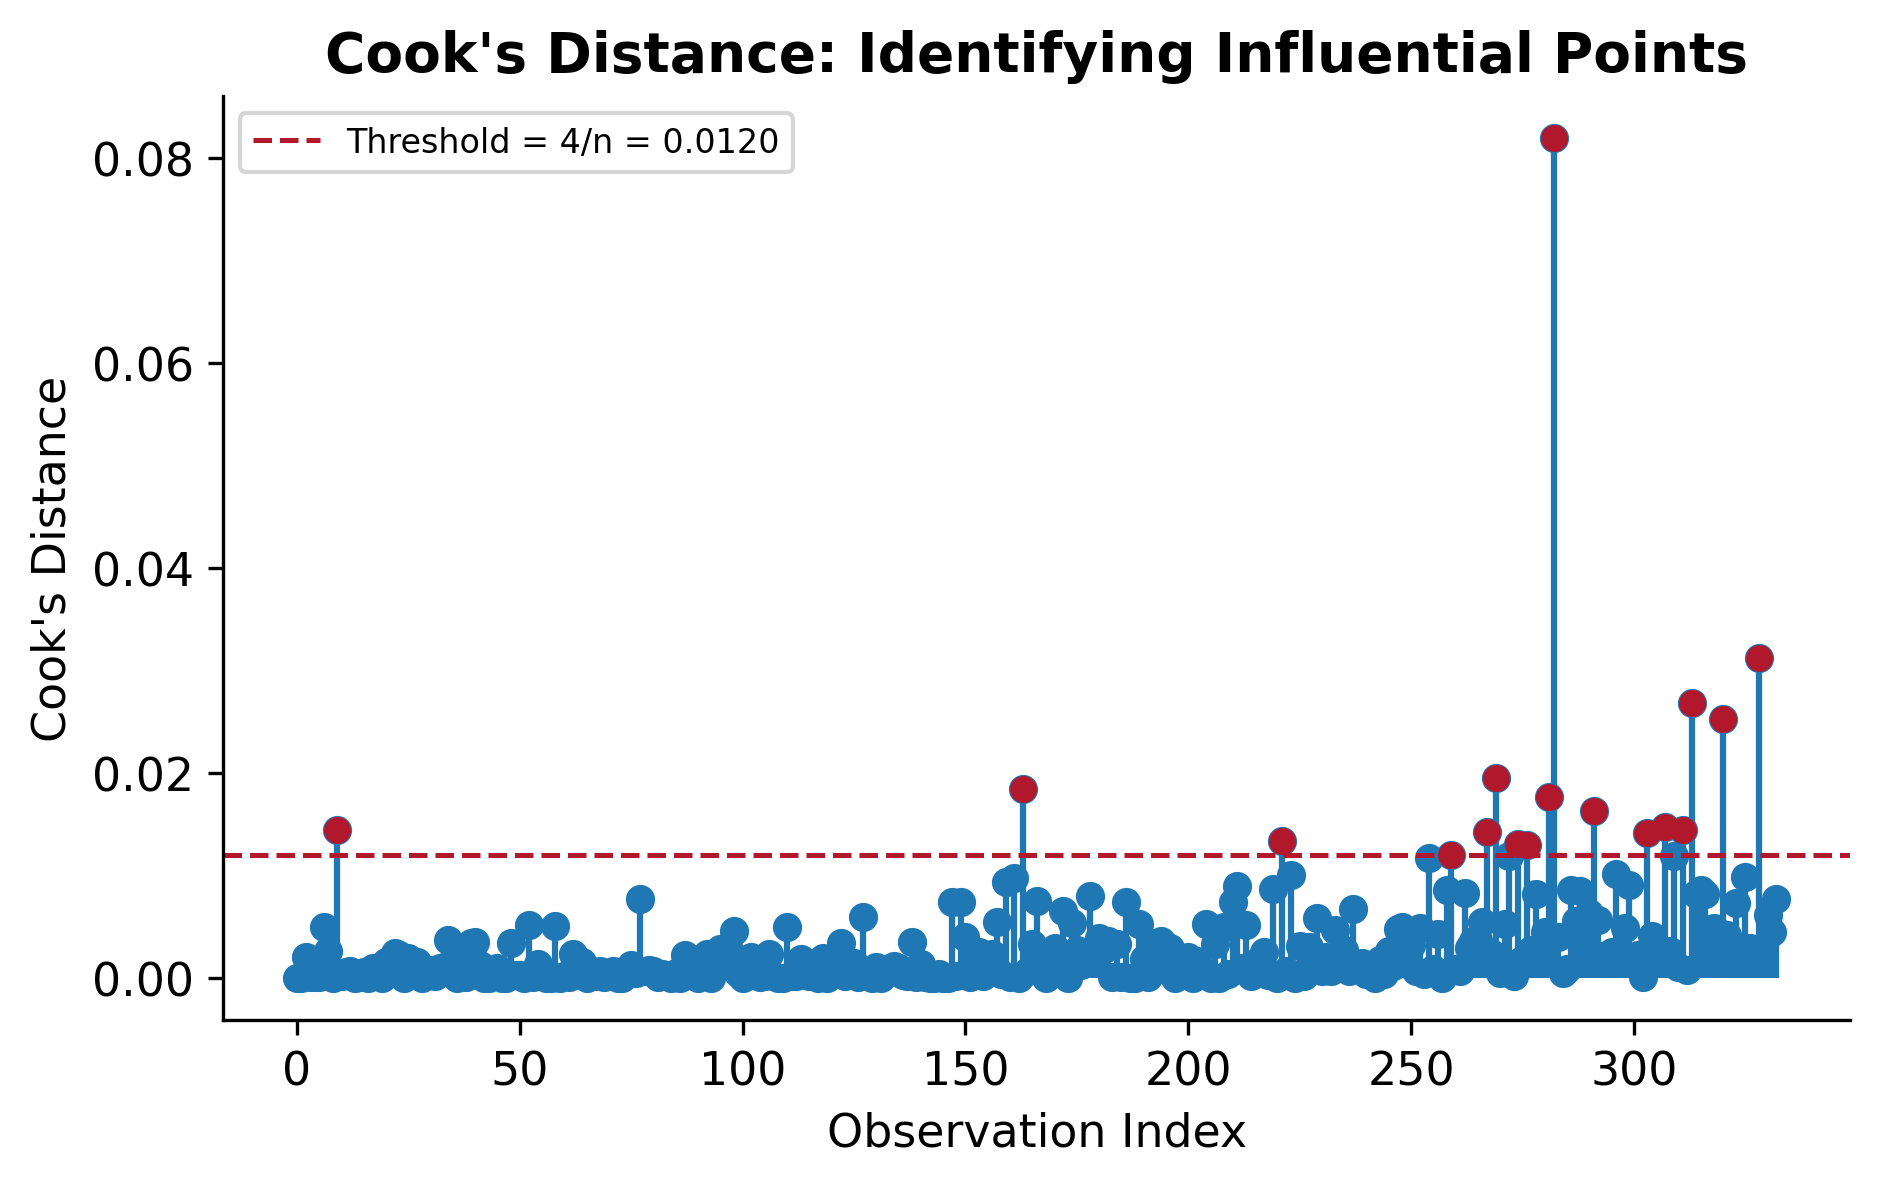
\includegraphics[width=0.72\textwidth]{m2_3_cooks_distance.png}

\vspace{0.2cm}
\begin{columns}[T]
\begin{column}{0.48\textwidth}
\begin{itemize}
    \item Measures how much \textbf{each observation changes the fit} if removed
    \item Combines leverage (unusual $x$) and residual (unusual $y | x$)
    \item Threshold: $D_i > 4/n$ (conservative) or $D_i > 1$ (liberal)
\end{itemize}
\end{column}
\begin{column}{0.48\textwidth}
\begin{exampleblock}{Data Insight}
    \scriptsize High Cook's $D$ does not mean ``delete this point.'' It means ``investigate this point.'' Influential observations may be the most scientifically interesting.
\end{exampleblock}
\end{column}
\end{columns}
\end{frame}

% ── 76 ──
\begin{frame}[fragile]{Cook's Distance --- Code}\smark{76/300}
\begin{columns}[T]
\begin{column}{0.48\textwidth}
\begin{lstlisting}[style=Rstyle]
model <- lm(y ~ x, data=df)

# Base R
plot(model, which = 4) # Cook's D

# ggplot2
library(broom)
diag <- augment(model)
ggplot(diag, aes(seq_along(.cooksd),
                 .cooksd)) +
  geom_col(fill="#2166AC") +
  geom_hline(yintercept=4/nrow(df),
    linetype="dashed",
    color="#B2182B") +
  labs(x="Obs", y="Cook's D")
\end{lstlisting}
\end{column}
\begin{column}{0.48\textwidth}
\begin{lstlisting}[style=Pystyle]
infl = model.get_influence()
cooks = infl.cooks_distance[0]

fig, ax = plt.subplots()
ax.stem(range(len(cooks)), cooks)
ax.axhline(4/len(cooks),
    linestyle="--", color="#B2182B")
ax.set_xlabel("Obs Index")
ax.set_ylabel("Cook's Distance")

# Identify influential
influential = np.where(
    cooks > 4/len(cooks))[0]
\end{lstlisting}
\vspace{0.1cm}
\begin{alertblock}{Pro-Tip}
    \scriptsize \texttt{broom::augment()} adds \texttt{.cooksd}, \texttt{.hat}, \texttt{.resid}, \texttt{.fitted} to the data frame --- ready for ggplot2.
\end{alertblock}
\end{column}
\end{columns}
\end{frame}

% ── 77 ──
\begin{frame}{Partial Regression and Component-Residual Plots}
\smark{77/300}
\centering
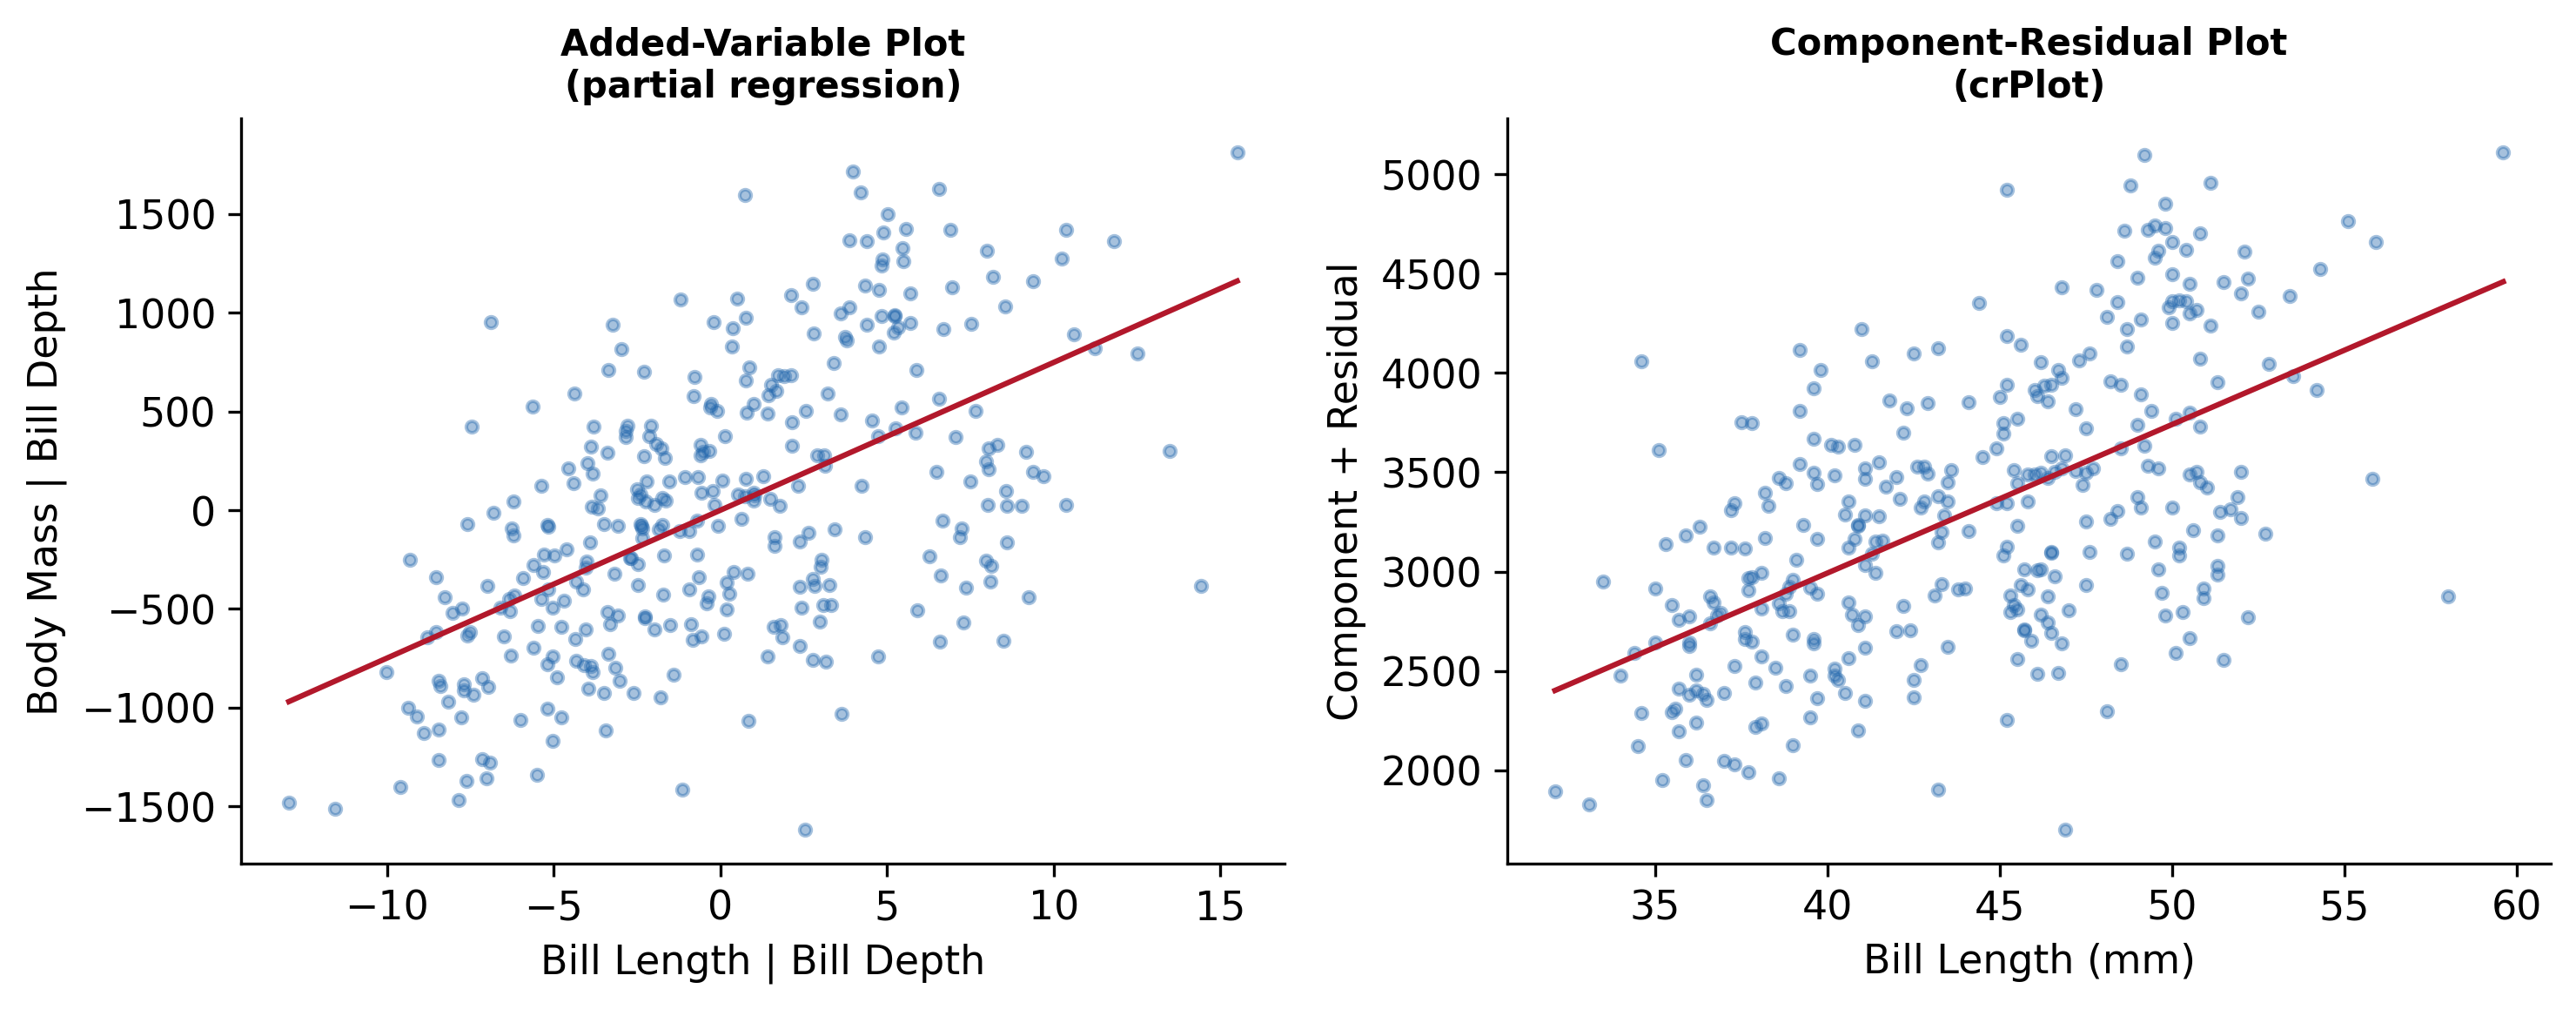
\includegraphics[width=0.88\textwidth]{m2_3_partial_regression.png}

\vspace{0.2cm}
\begin{columns}[T]
\begin{column}{0.48\textwidth}
\begin{exampleblock}{Data Insight}
    \scriptsize Left: added-variable plot shows the \textbf{unique} contribution of bill length after controlling for bill depth. Right: component-residual plot checks \textbf{linearity} of each predictor in the multivariate model.
\end{exampleblock}
\end{column}
\begin{column}{0.48\textwidth}
\begin{alertblock}{Pro-Tip}
    \scriptsize R: \texttt{car::avPlots(model)} for added-variable; \texttt{car::crPlots(model)} for component-residual. Python: \texttt{sm.graphics.plot\_partregress()} and \texttt{plot\_ccpr()}.
\end{alertblock}
\end{column}
\end{columns}
\end{frame}

% ── 78 ──
\begin{frame}[fragile]{Partial Regression --- Code}\smark{78/300}
\begin{columns}[T]
\begin{column}{0.48\textwidth}
\begin{lstlisting}[style=Rstyle]
model <- lm(body_mass_g ~
  bill_length_mm + bill_depth_mm,
  data = penguins)

# Added-variable plots
library(car)
avPlots(model)

# Component-residual plots
crPlots(model)

# ggplot2 via ggfortify
library(ggfortify)
autoplot(model, which = 1:6)
\end{lstlisting}
\end{column}
\begin{column}{0.48\textwidth}
\begin{lstlisting}[style=Pystyle]
import statsmodels.api as sm

# Added-variable
fig = sm.graphics.plot_partregress(
    "body_mass_g",
    "bill_length_mm",
    ["bill_depth_mm"],
    data=penguins)

# Component + residual
fig = sm.graphics.plot_ccpr(
    model, "bill_length_mm")

# All partial plots at once
fig = sm.graphics \
    .plot_partregress_grid(model)
\end{lstlisting}
\end{column}
\end{columns}
\end{frame}

% ── 79 ──
\begin{frame}{Smoother Comparison}
\smark{79/300}
\centering
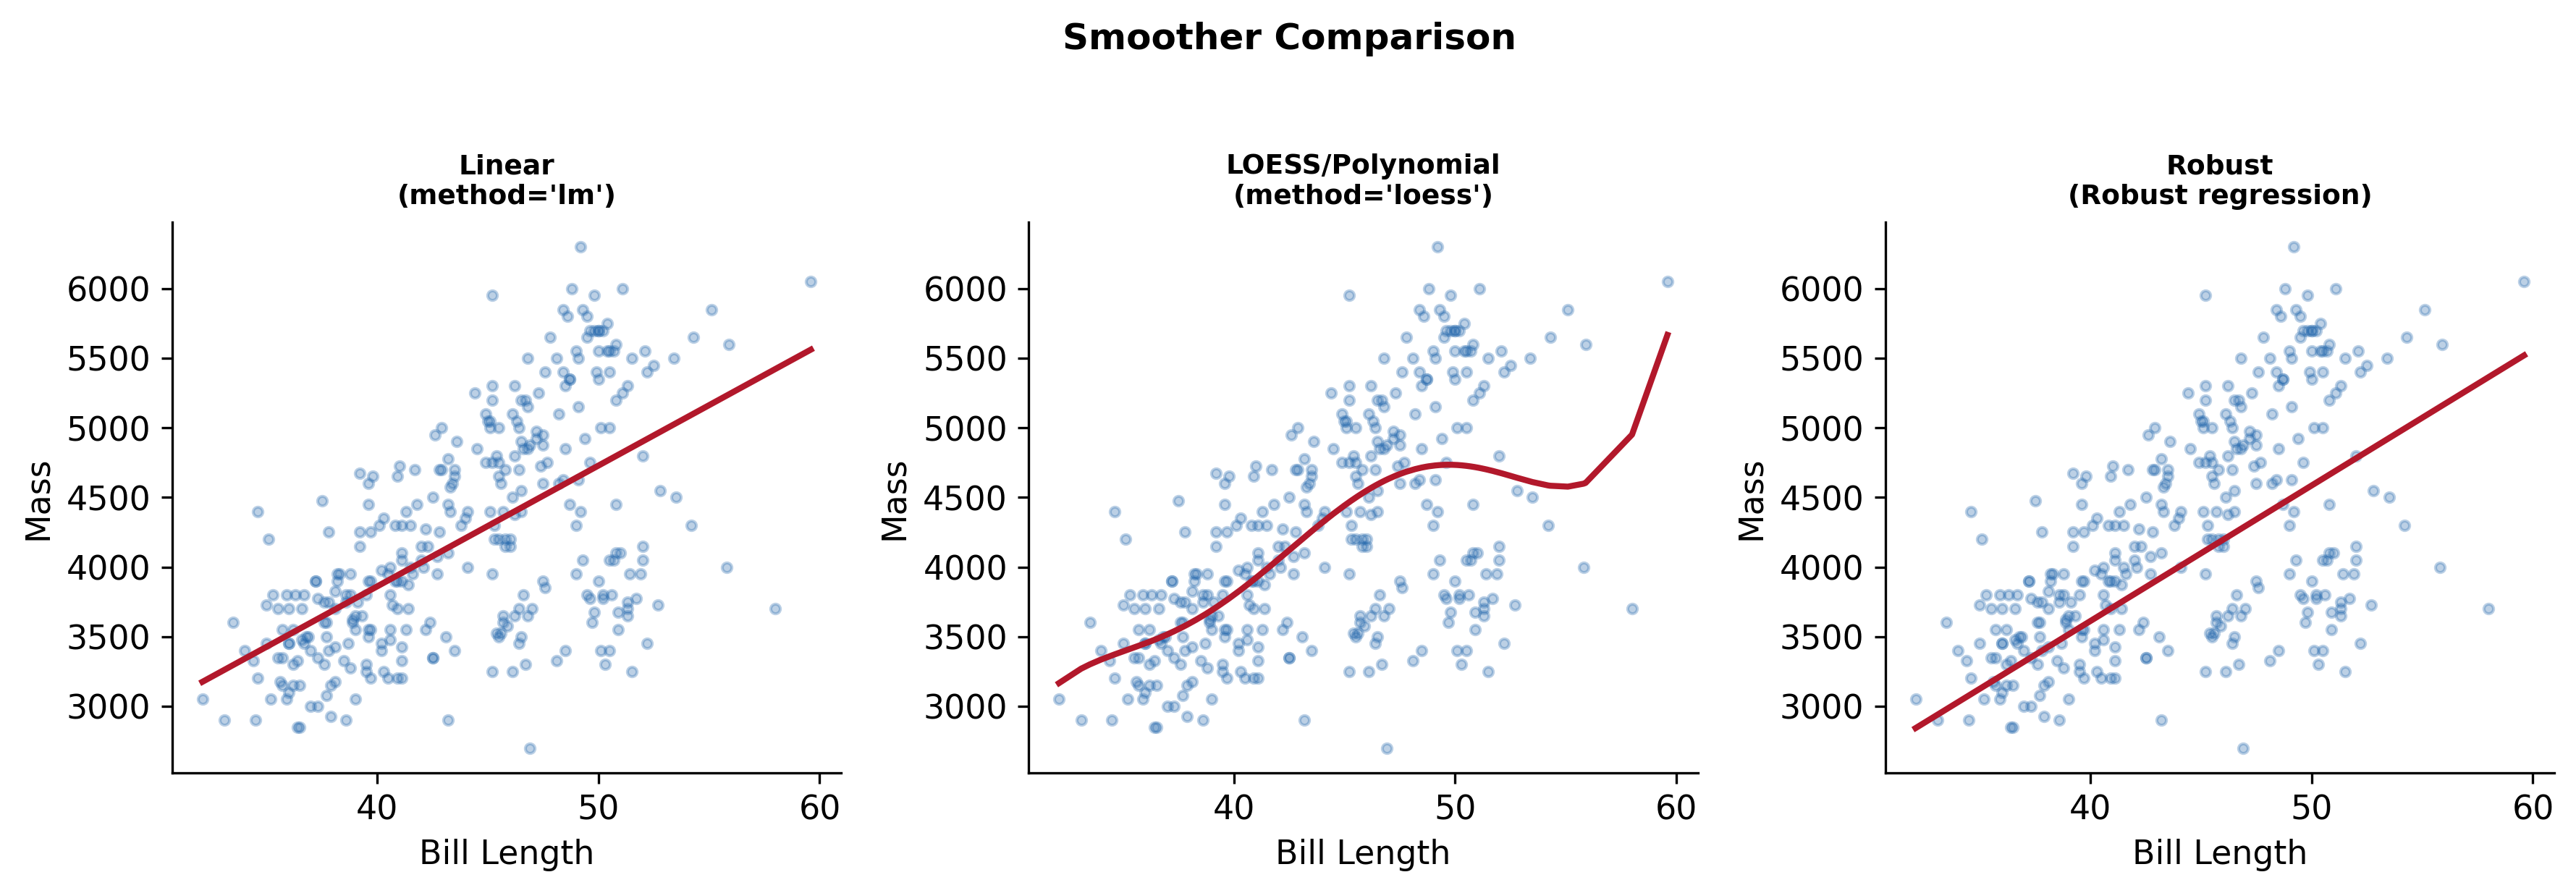
\includegraphics[width=0.88\textwidth]{m2_3_smooth_types.png}

\vspace{0.2cm}
\centering\small
\begin{tabular}{@{}llll@{}}
    \toprule
    \textbf{Smoother} & \textbf{R} & \textbf{Python} & \textbf{Use} \\
    \midrule
    OLS linear  & \texttt{method="lm"}   & \texttt{regplot(order=1)} & Inference, slopes \\
    LOESS/poly  & \texttt{method="loess"} & \texttt{lowess=True}     & EDA, non-linearity \\
    GAM         & \texttt{method="gam"}  & \texttt{pygam}            & Smooth non-linear \\
    Robust      & \texttt{MASS::rlm()}   & Theil--Sen / HuberReg    & Outlier-resistant \\
    \bottomrule
\end{tabular}
\end{frame}

% ── 80 ──
\begin{frame}[fragile]{Smoother --- \Rlang}\smark{80/300}
\begin{columns}[T]
\begin{column}{0.55\textwidth}
\begin{lstlisting}[style=Rstyle]
# OLS (default for lm)
geom_smooth(method = "lm")

# LOESS (default for n<1000)
geom_smooth(method = "loess",
  span = 0.75)  # span = bandwidth

# GAM (for large n)
geom_smooth(method = "gam",
  formula = y ~ s(x, bs = "cs"))

# Robust
library(MASS)
geom_smooth(method = "rlm")
# Uses M-estimation (Huber)
\end{lstlisting}
\end{column}
\begin{column}{0.42\textwidth}
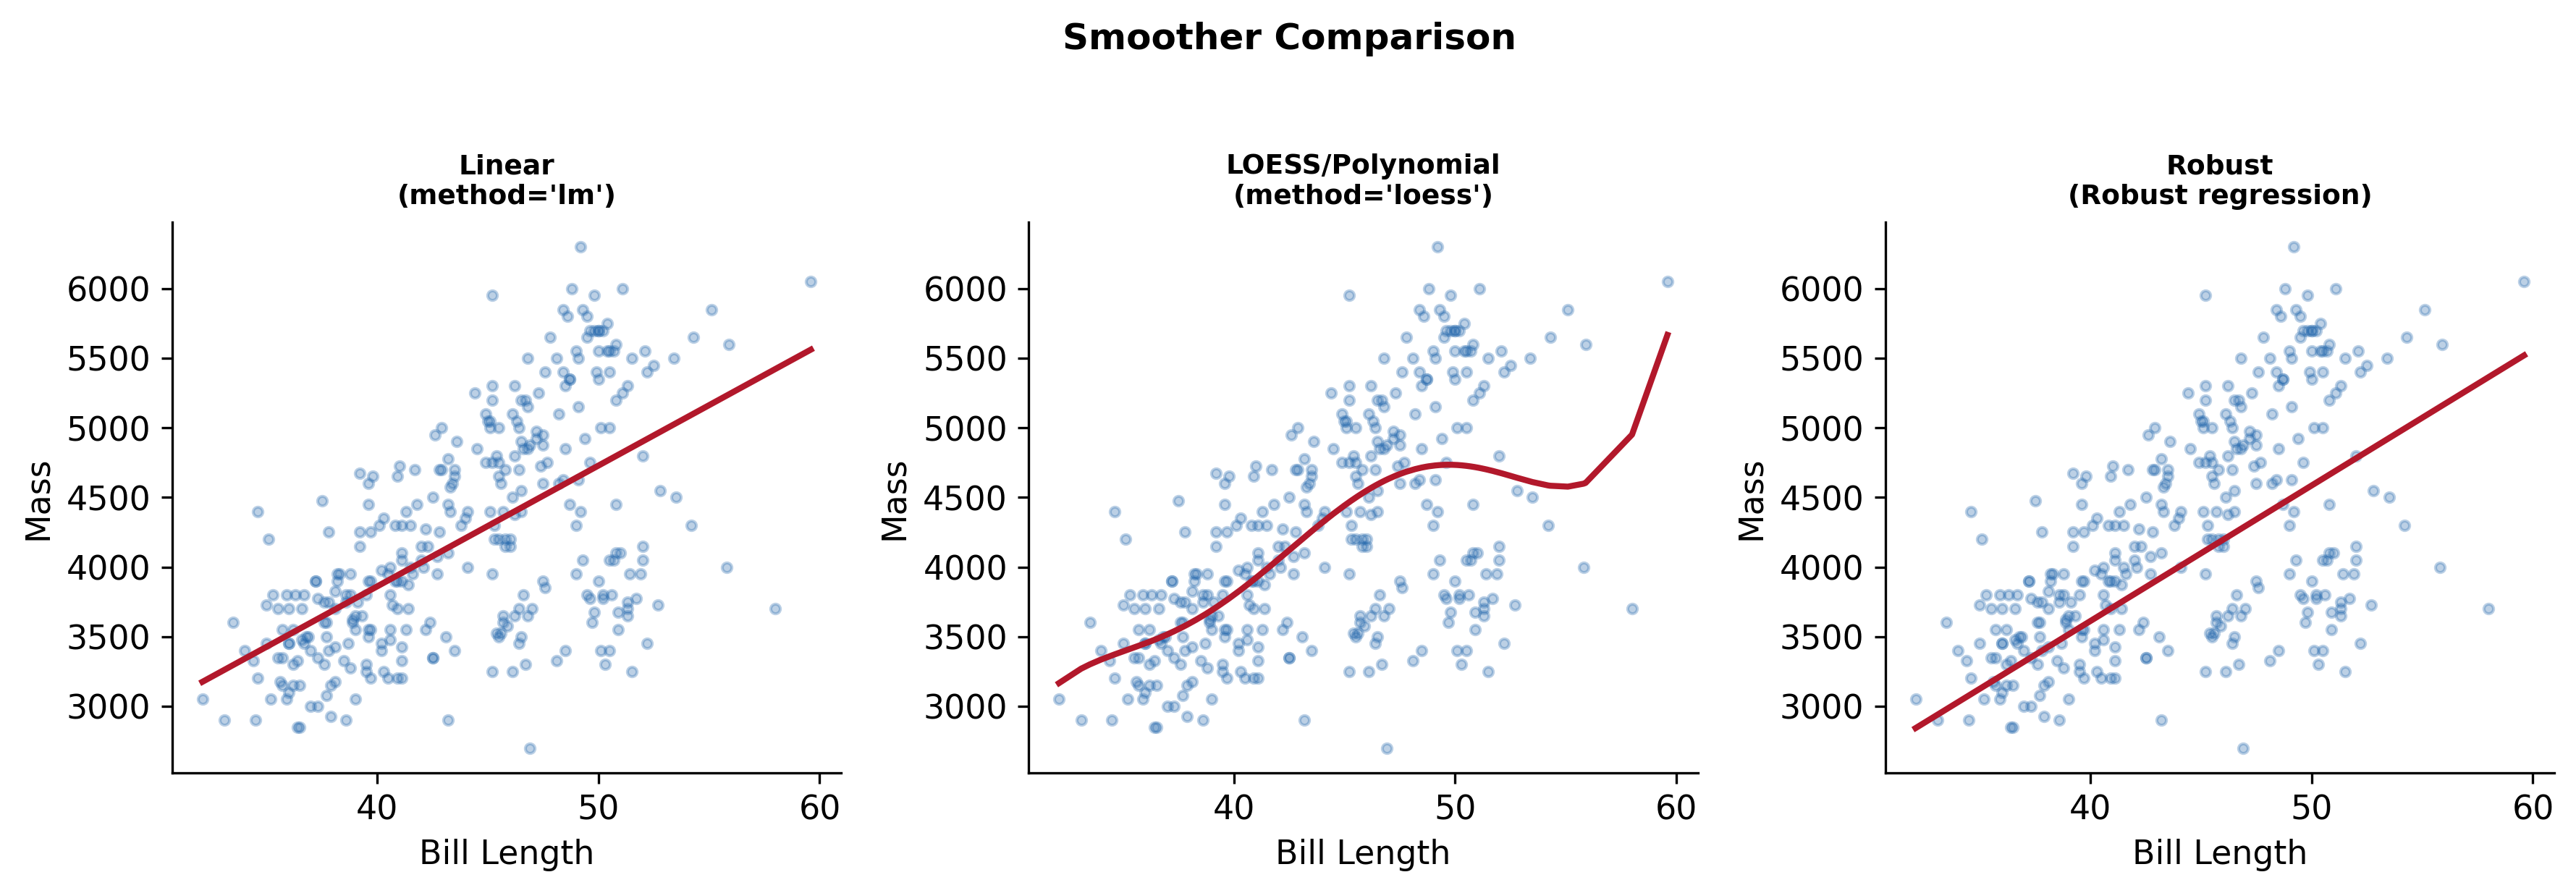
\includegraphics[width=\textwidth]{m2_3_smooth_types.png}
\begin{alertblock}{Pro-Tip}
    \scriptsize \texttt{span=} controls LOESS bandwidth (like KDE's \texttt{adjust}). Smaller span $\to$ wigglier curve. Default 0.75 is usually fine. For GAMs, use \texttt{bs="cs"} (cubic splines).
\end{alertblock}
\end{column}
\end{columns}
\end{frame}

% ── 81 ──
\begin{frame}[fragile]{Smoother --- \Python}\smark{81/300}
\begin{columns}[T]
\begin{column}{0.55\textwidth}
\begin{lstlisting}[style=Pystyle]
# seaborn: OLS
sns.regplot(data=df, x="x", y="y",
    ci=95)  # default linear

# seaborn: LOWESS
sns.regplot(data=df, x="x", y="y",
    lowess=True)

# seaborn: polynomial
sns.regplot(data=df, x="x", y="y",
    order=3)

# plotnine
(ggplot(df, aes("x","y"))
 + geom_smooth(method="lm"))
(ggplot(df, aes("x","y"))
 + geom_smooth(method="loess",
     span=0.5))
\end{lstlisting}
\end{column}
\begin{column}{0.42\textwidth}
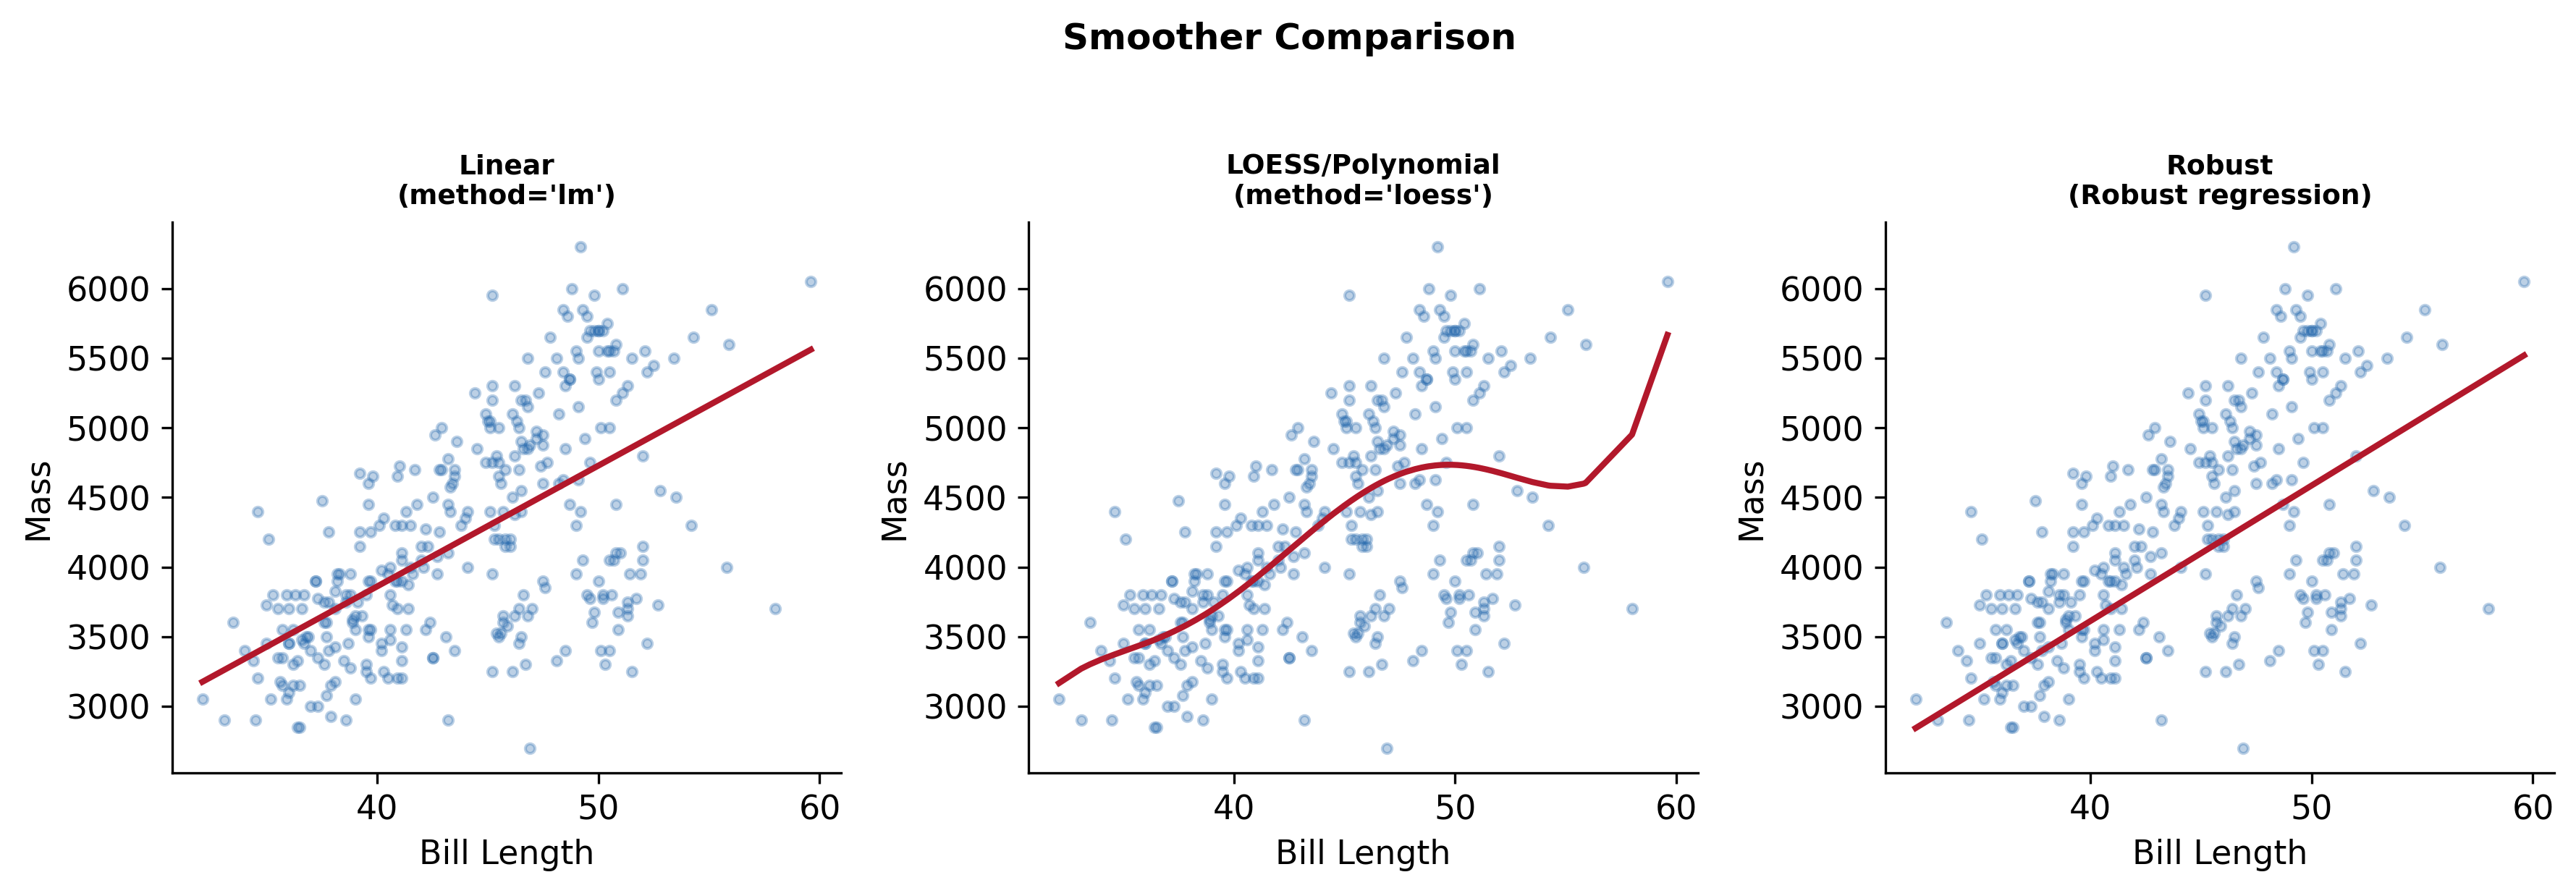
\includegraphics[width=\textwidth]{m2_3_smooth_types.png}
\begin{exampleblock}{Data Insight}
    \scriptsize \texttt{sns.regplot(lowess=True)} uses LOWESS. \texttt{order=n} fits a polynomial of degree $n$. For GAMs in Python, install \texttt{pygam} and fit manually.
\end{exampleblock}
\end{column}
\end{columns}
\end{frame}

% ── 82 ──
\begin{frame}{Grouped Regression: Separate Lines per Group}
\smark{82/300}
\begin{columns}[T]
\begin{column}{0.50\textwidth}
\begin{itemize}
    \item Map \texttt{color=group} inside \texttt{aes()} --- \texttt{geom\_smooth()} fits a separate line per group
    \item Reveals whether the relationship differs across categories
    \item Simpson's paradox: pooled trend can reverse within groups
    \item Module 2.5 covers interaction visualization in depth
\end{itemize}
\end{column}
\begin{column}{0.47\textwidth}
\begin{exampleblock}{Data Insight}
    \scriptsize Penguin bill length vs.\ body mass: the pooled OLS line shows a positive slope. But \emph{within} Adelie, the slope is much steeper. Color reveals the group-level story.
\end{exampleblock}
\vspace{0.1cm}
\begin{alertblock}{Pro-Tip}
    \scriptsize In seaborn: \texttt{sns.lmplot(hue="species")} fits separate regressions automatically. In matplotlib, loop over groups and call \texttt{np.polyfit()} per group.
\end{alertblock}
\end{column}
\end{columns}
\end{frame}

% ── 83 ──
\begin{frame}[fragile]{Grouped Regression --- Code}\smark{83/300}
\begin{columns}[T]
\begin{column}{0.48\textwidth}
\begin{lstlisting}[style=Rstyle]
ggplot(penguins,
  aes(bill_length_mm,
      body_mass_g,
      color = species)) +
  geom_point(alpha = 0.4) +
  geom_smooth(method = "lm",
    se = FALSE) +
  scale_color_manual(
    values=c("#1B9E77","#D95F02",
             "#7570B3")) +
  theme_minimal()
# One line per species
\end{lstlisting}
\end{column}
\begin{column}{0.48\textwidth}
\begin{lstlisting}[style=Pystyle]
# seaborn: hue = separate fits
sns.lmplot(data=penguins,
    x="bill_length_mm",
    y="body_mass_g",
    hue="species", ci=None,
    palette=["#1B9E77","#D95F02",
             "#7570B3"],
    height=4, aspect=1.3)

# plotnine
(ggplot(penguins, aes(
    "bill_length_mm","body_mass_g",
    color="species"))
 + geom_point(alpha=0.4)
 + geom_smooth(method="lm",
     se=False))
\end{lstlisting}
\end{column}
\end{columns}
\end{frame}

% ── 84 ──
\begin{frame}{Residual Diagnostic Summary Table}
\smark{84/300}
\centering\small
\begin{tabular}{@{}llll@{}}
    \toprule
    \textbf{Pattern} & \textbf{Problem} & \textbf{Fix} & \textbf{R Function} \\
    \midrule
    Curve in residuals       & Non-linearity     & Polynomial / GAM        & \texttt{crPlots()} \\
    Funnel in residuals      & Heteroscedasticity& Log $y$ / WLS / robust SE& \texttt{bptest()} \\
    Heavy tails on QQ        & Non-normality     & Bootstrap CIs           & \texttt{qqPlot()} \\
    High Cook's $D$          & Influential point & Investigate, sensitivity& \texttt{influencePlot()} \\
    High leverage + residual & Outlier + leverage& Robust regression       & \texttt{rlm()} \\
    Correlated residuals     & Autocorrelation   & GLS / time-series model & \texttt{dwtest()} \\
    \bottomrule
\end{tabular}

\vspace{0.3cm}
\begin{alertblock}{Pro-Tip}
    \scriptsize Diagnostic plots are \textbf{sequential}: fix non-linearity first, then re-check heteroscedasticity and normality. Many apparent normality failures are actually non-linearity artifacts.
\end{alertblock}
\end{frame}

% ── 85 ──
\begin{frame}{Coefficient Plots: Visualizing Regression Tables}
\smark{85/300}
\begin{columns}[T]
\begin{column}{0.50\textwidth}
\begin{itemize}
    \item Point = estimated coefficient
    \item Horizontal line = 95\% CI
    \item Vertical dashed line at $\beta = 0$ (null hypothesis)
    \item If CI crosses zero $\to$ not significant at 5\%
    \item Much easier to read than a regression table
\end{itemize}
\end{column}
\begin{column}{0.47\textwidth}
\begin{exampleblock}{Data Insight}
    \scriptsize Coefficient plots replace the ``stargazer table'' for presentations. The visual immediately shows which predictors matter and their relative magnitude.
\end{exampleblock}
\vspace{0.1cm}
\begin{alertblock}{Pro-Tip}
    \scriptsize R: \texttt{dotwhisker::dwplot(model)} or \texttt{sjPlot::plot\_model(model)}. Python: \texttt{forestplot} package, or manual \texttt{ax.errorbar()}.
\end{alertblock}
\end{column}
\end{columns}
\end{frame}

% ── 86 ──
\begin{frame}[fragile]{Coefficient Plot --- Code}\smark{86/300}
\begin{columns}[T]
\begin{column}{0.48\textwidth}
\begin{lstlisting}[style=Rstyle]
library(broom)
library(ggplot2)

model <- lm(body_mass_g ~
  bill_length_mm + bill_depth_mm +
  flipper_length_mm,
  data = penguins)

tidy(model, conf.int=TRUE) |>
  filter(term != "(Intercept)") |>
  ggplot(aes(estimate, term)) +
  geom_pointrange(
    aes(xmin=conf.low,
        xmax=conf.high)) +
  geom_vline(xintercept=0,
    linetype="dashed",
    color="#B2182B") +
  theme_minimal()
\end{lstlisting}
\end{column}
\begin{column}{0.48\textwidth}
\begin{lstlisting}[style=Pystyle]
params = model.params[1:]
ci = model.conf_int().iloc[1:]

fig, ax = plt.subplots()
ax.errorbar(params, range(len(params)),
    xerr=[params - ci[0],
          ci[1] - params],
    fmt="o", capsize=5,
    color="#2166AC", markersize=8)
ax.axvline(0, linestyle="--",
    color="#B2182B")
ax.set_yticks(range(len(params)))
ax.set_yticklabels(params.index)
ax.set_xlabel("Coefficient Estimate")
\end{lstlisting}
\end{column}
\end{columns}
\end{frame}

% ── 87 ──
\begin{frame}{Multiple Model Comparison}
\smark{87/300}
\begin{columns}[T]
\begin{column}{0.50\textwidth}
\begin{itemize}
    \item Plot coefficients from 2+ models side by side
    \item Shows how estimates \textbf{change} as covariates are added
    \item Reveals confounding: if $\beta$ shifts when a covariate enters, that covariate confounds the relationship
    \item R: \texttt{dotwhisker::dwplot(list(m1, m2, m3))}
\end{itemize}
\end{column}
\begin{column}{0.47\textwidth}
\begin{exampleblock}{Data Insight}
    \scriptsize If bill\_length's coefficient halves when species is added, species is a confounder. The visual comparison across models makes this pattern obvious; a regression table buries it in columns of numbers.
\end{exampleblock}
\end{column}
\end{columns}
\end{frame}

% ── 88 ──
\begin{frame}[fragile]{Multi-Model Coefficient Plot --- Code}\smark{88/300}
\begin{columns}[T]
\begin{column}{0.48\textwidth}
\begin{lstlisting}[style=Rstyle]
library(dotwhisker)

m1 <- lm(body_mass_g ~
  bill_length_mm, data=penguins)
m2 <- lm(body_mass_g ~
  bill_length_mm + species,
  data=penguins)
m3 <- lm(body_mass_g ~
  bill_length_mm + species +
  flipper_length_mm,
  data=penguins)

dwplot(list(m1, m2, m3)) +
  geom_vline(xintercept=0,
    linetype="dashed") +
  theme_minimal()
\end{lstlisting}
\end{column}
\begin{column}{0.48\textwidth}
\begin{lstlisting}[style=Pystyle]
# Manual multi-model
models = {"Simple": m1,
          "+Species": m2,
          "+Flipper": m3}

fig, ax = plt.subplots()
for i, (name, m) in enumerate(
    models.items()):
    params = m.params[1:3]
    ci = m.conf_int().iloc[1:3]
    y_pos = np.arange(len(params))\
            + i*0.15
    ax.errorbar(params, y_pos,
        xerr=[params-ci[0],
              ci[1]-params],
        fmt="o", capsize=4,
        label=name)
ax.axvline(0, linestyle="--")
ax.legend()
\end{lstlisting}
\end{column}
\end{columns}
\end{frame}

% ── 89 ──
\begin{frame}{When to Use Which Diagnostic Plot}
\smark{89/300}
\centering\small
\begin{tabular}{@{}lll@{}}
    \toprule
    \textbf{Question} & \textbf{Plot} & \textbf{Tool} \\
    \midrule
    Is the relationship linear?    & Residuals vs.\ Fitted  & \texttt{plot(lm, 1)} \\
    Are residuals normal?          & Q-Q of residuals        & \texttt{plot(lm, 2)} \\
    Is variance constant?          & Scale-Location          & \texttt{plot(lm, 3)} \\
    Any influential points?        & Cook's $D$ stem plot    & \texttt{plot(lm, 4)} \\
    Predictor linearity (multi)?   & Component-residual      & \texttt{car::crPlots()} \\
    Unique predictor contribution? & Added-variable          & \texttt{car::avPlots()} \\
    Overall coefficient comparison?& Coefficient / forest    & \texttt{dotwhisker::dwplot()} \\
    \bottomrule
\end{tabular}
\end{frame}

% ── 90 ──
\begin{frame}{Module 2.3 --- Key Takeaways}\smark{90/300}
\begin{enumerate}
    \item \textbf{Always plot diagnostics} after fitting any regression.
    \item \textbf{Residuals vs.\ fitted} catches non-linearity and heteroscedasticity.
    \item \textbf{Q-Q plot of residuals} checks normality; moderate violations are tolerable with large $n$.
    \item \textbf{Cook's distance} flags influential points --- investigate, don't auto-delete.
    \item \textbf{CI $\neq$ PI}. CI = mean response, PI = new observation. PI is always wider.
    \item \textbf{Coefficient plots} replace regression tables for presentations.
\end{enumerate}
\end{frame}

% ── 91 ──
\begin{frame}{}\smark{91/300}
\centering\vspace{1.5cm}
{\Large\textbf{Module 2.3 Complete}}\\[0.5cm]
You can now visually assess every OLS assumption --- linearity, normality, homoscedasticity, influence --- and present model results with coefficient plots instead of tables.\\[0.5cm]
\textbf{Next:} Module 2.4 --- Uncertainty Visualization: Error Bars, Intervals, and Bands.
\end{frame}

% ═══════════════════════════════════════════════════════
%  MODULE 2.4 — Uncertainty Visualization: Error Bars, Intervals, and Bands
% ═══════════════════════════════════════════════════════
\section{Module 2.4 --- Uncertainty Visualization}

% ── 92 ──
\begin{frame}{Module 2.4 --- Roadmap}\smark{92/300}
\begin{enumerate}
    \item Why uncertainty visualization matters
    \item Five representations: error bars, gradient, violin, HOPs, quantile dots
    \item Ribbon bands for time series
    \item Fan charts: gradient intervals for forecasts
    \item Forest plots for meta-analysis and multi-study comparison
    \item Slab + interval (ggdist) as the modern standard
    \item Bayesian posteriors and HDI
    \item Hypothetical Outcome Plots (HOPs)
\end{enumerate}
\end{frame}

% ── 93 ──
\begin{frame}{Why Uncertainty Visualization Matters}
\smark{93/300}
\begin{columns}[T]
\begin{column}{0.50\textwidth}
\begin{itemize}
    \item A point estimate without uncertainty is a \textbf{lie of precision}
    \item People systematically \textbf{underweight} uncertainty when shown only bars + error bars
    \item Animated and gradient displays improve uncertainty calibration (Hullman et al., 2015)
    \item Scientific reporting increasingly \textbf{requires} uncertainty displays
\end{itemize}
\end{column}
\begin{column}{0.47\textwidth}
\begin{exampleblock}{Data Insight}
    \scriptsize Joslyn \& LeClerc (2012): people make better decisions when shown full distributional uncertainty (e.g., rain probability range) vs.\ point forecasts (``30\% chance of rain'').
\end{exampleblock}
\vspace{0.2cm}
\begin{alertblock}{Pro-Tip}
    \scriptsize The choice of uncertainty representation \textbf{changes what people conclude from the same data}. This is not merely aesthetic --- it is inferential.
\end{alertblock}
\end{column}
\end{columns}
\end{frame}

% ── 94 ──
\begin{frame}{Five Ways to Show Uncertainty}
\smark{94/300}
\centering
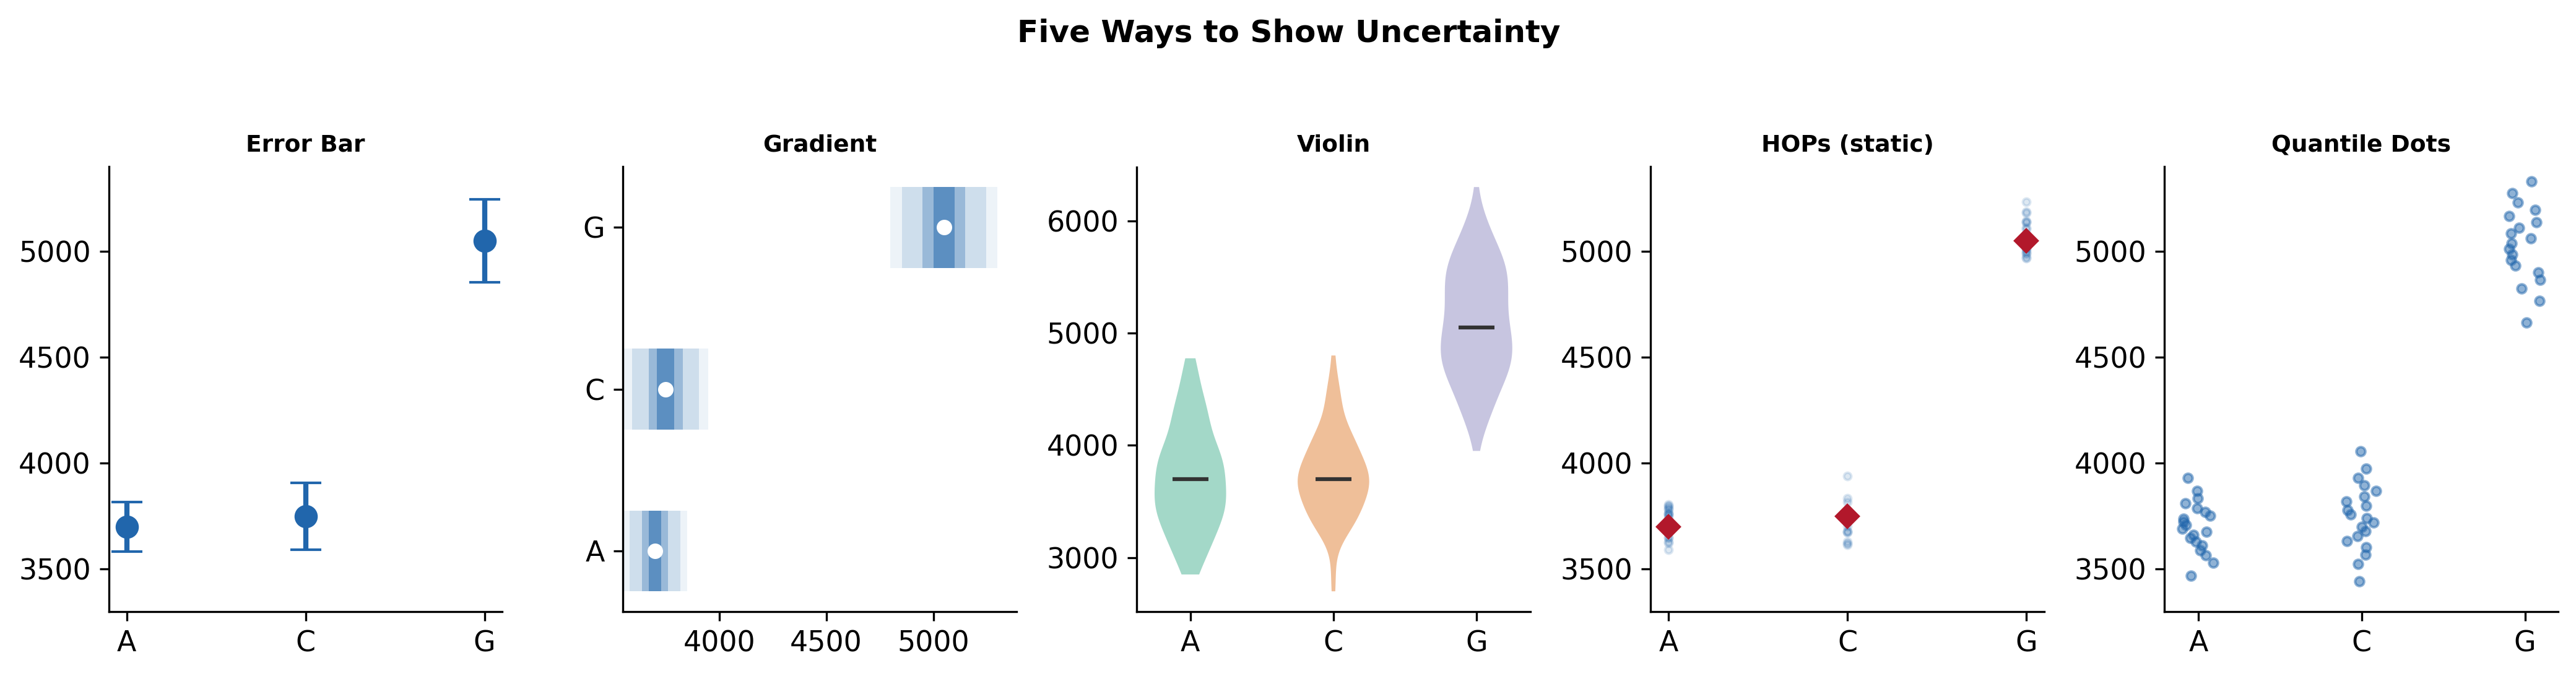
\includegraphics[width=0.95\textwidth]{m2_4_uncertainty_palette.png}

\vspace{0.2cm}
\begin{exampleblock}{Data Insight}
    \scriptsize Same data, five encodings. Error bars are most familiar but encode only two numbers ($\pm$). Gradient and violin show the full shape. HOPs and quantile dots engage probability intuition directly.
\end{exampleblock}
\end{frame}

% ── 95 ──
\begin{frame}{Uncertainty Representation Comparison}
\smark{95/300}
\centering\small
\begin{tabular}{@{}llll@{}}
    \toprule
    \textbf{Type} & \textbf{Shows} & \textbf{Strength} & \textbf{Weakness} \\
    \midrule
    Error bar       & $\pm$ 1 interval       & Familiar, compact   & Hides shape \\
    Gradient        & Multiple quantiles     & Shows density decay  & Needs explanation \\
    Violin / slab   & Full density           & Shape visible        & Uncommon to non-experts \\
    HOPs (animated) & Bootstrap draws        & Intuitive probability& Requires animation \\
    Quantile dots   & Discrete probability   & Countable outcomes   & Unfamiliar format \\
    \bottomrule
\end{tabular}

\vspace{0.3cm}
\begin{alertblock}{Pro-Tip}
    \scriptsize For expert audiences: slab + interval (ggdist). For general public: gradient intervals or HOPs. Error bars are the minimum viable uncertainty display.
\end{alertblock}
\end{frame}

% ── 96 ──
\begin{frame}{The Slab + Interval: Modern Standard}
\smark{96/300}
\centering
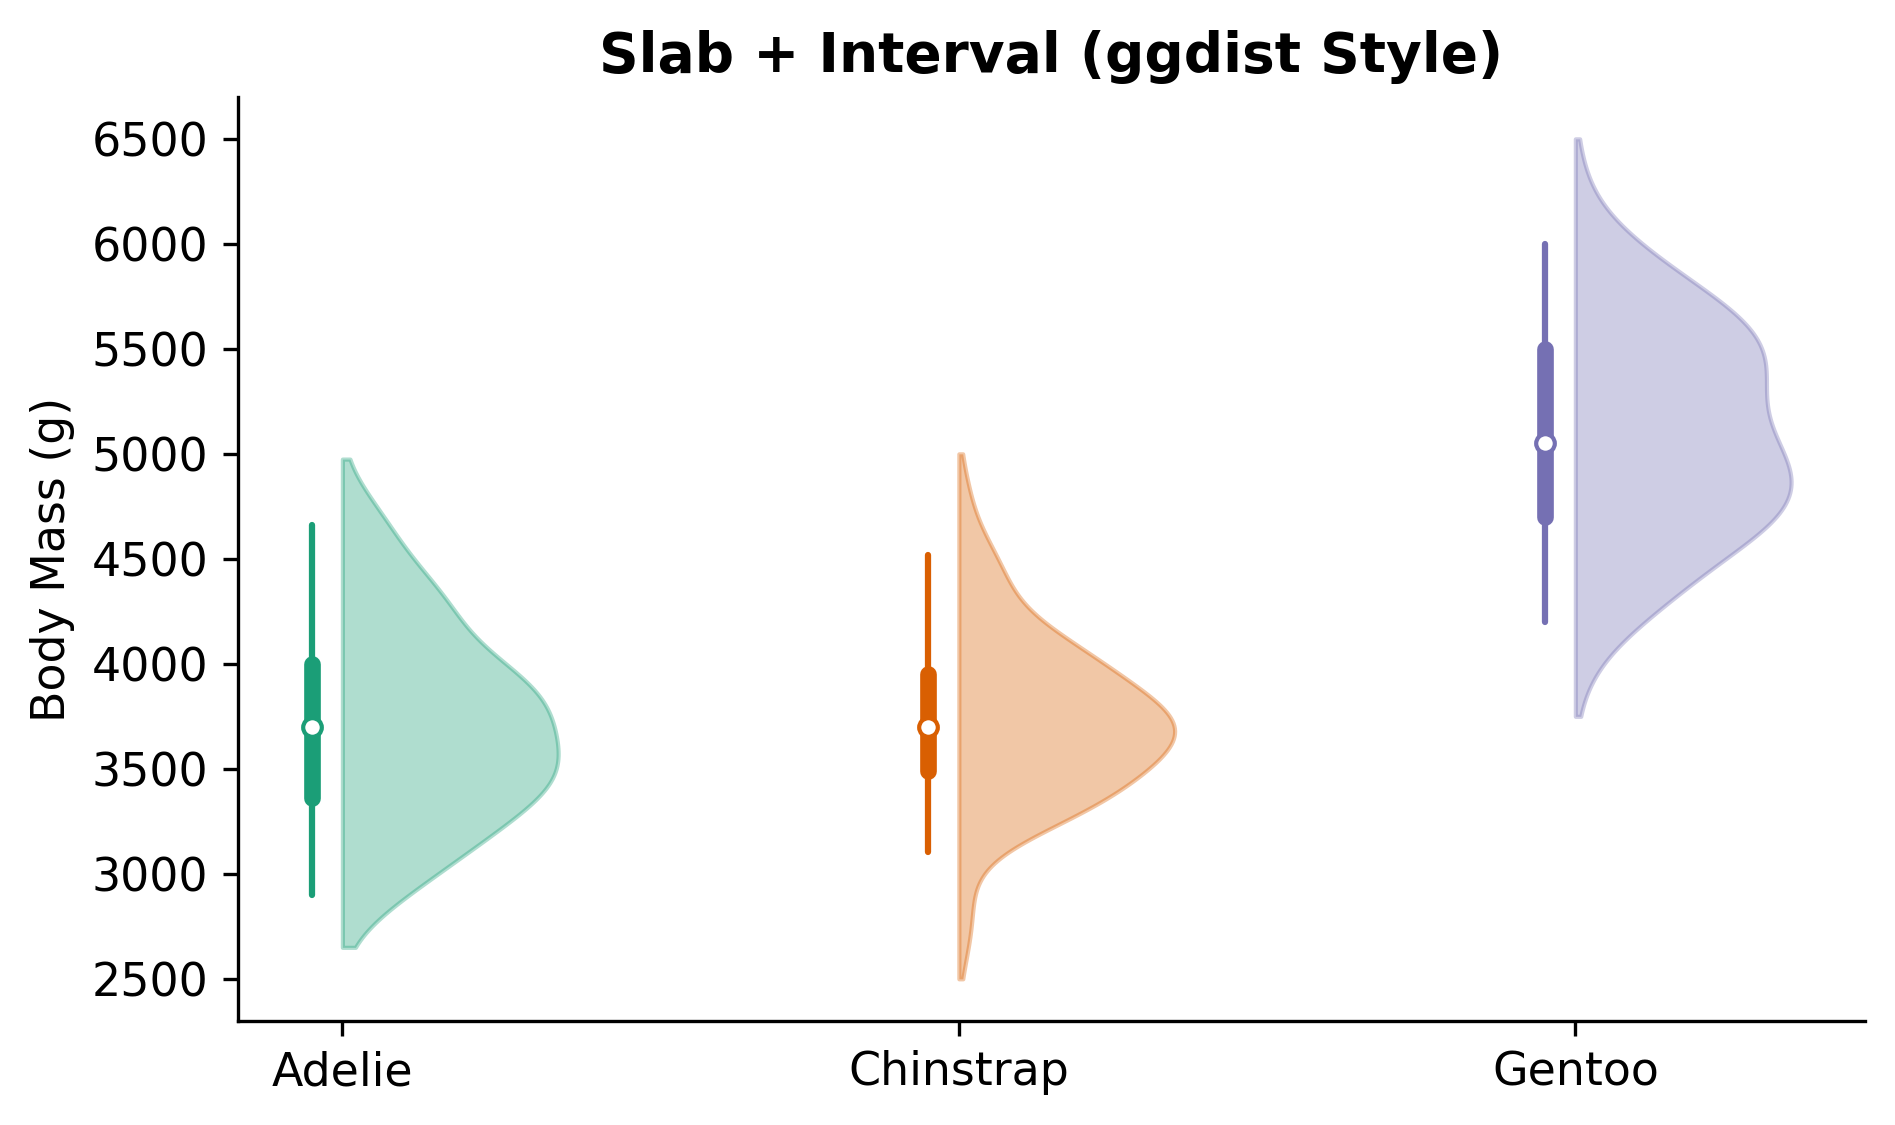
\includegraphics[width=0.68\textwidth]{m2_4_slab_interval.png}

\vspace{0.2cm}
\begin{columns}[T]
\begin{column}{0.48\textwidth}
\begin{itemize}
    \item \textbf{Slab} = half-density curve (shape)
    \item \textbf{Thick bar} = IQR (25th--75th)
    \item \textbf{Thin bar} = 95\% interval
    \item \textbf{Point} = median
    \item Introduced by \texttt{ggdist} (Kay, 2024)
\end{itemize}
\end{column}
\begin{column}{0.48\textwidth}
\begin{exampleblock}{Data Insight}
    \scriptsize The slab + interval encodes \textbf{three levels of information} simultaneously: full shape, credible interval, and point estimate. It is the gold standard for Bayesian and frequentist reporting.
\end{exampleblock}
\end{column}
\end{columns}
\end{frame}

% ── 97 ──
\begin{frame}[fragile]{Slab + Interval --- \Rlang}\smark{97/300}
\begin{columns}[T]
\begin{column}{0.55\textwidth}
\begin{lstlisting}[style=Rstyle]
library(ggdist)

ggplot(penguins,
  aes(species, body_mass_g,
      fill = species)) +
  stat_halfeye(
    # Slab (density)
    .width = c(0.5, 0.95),
    # Interval (thick + thin)
    point_interval = median_qi,
    slab_alpha = 0.35) +
  scale_fill_manual(
    values=c("#1B9E77","#D95F02",
             "#7570B3")) +
  theme_minimal() +
  theme(legend.position="none")
\end{lstlisting}
\end{column}
\begin{column}{0.42\textwidth}
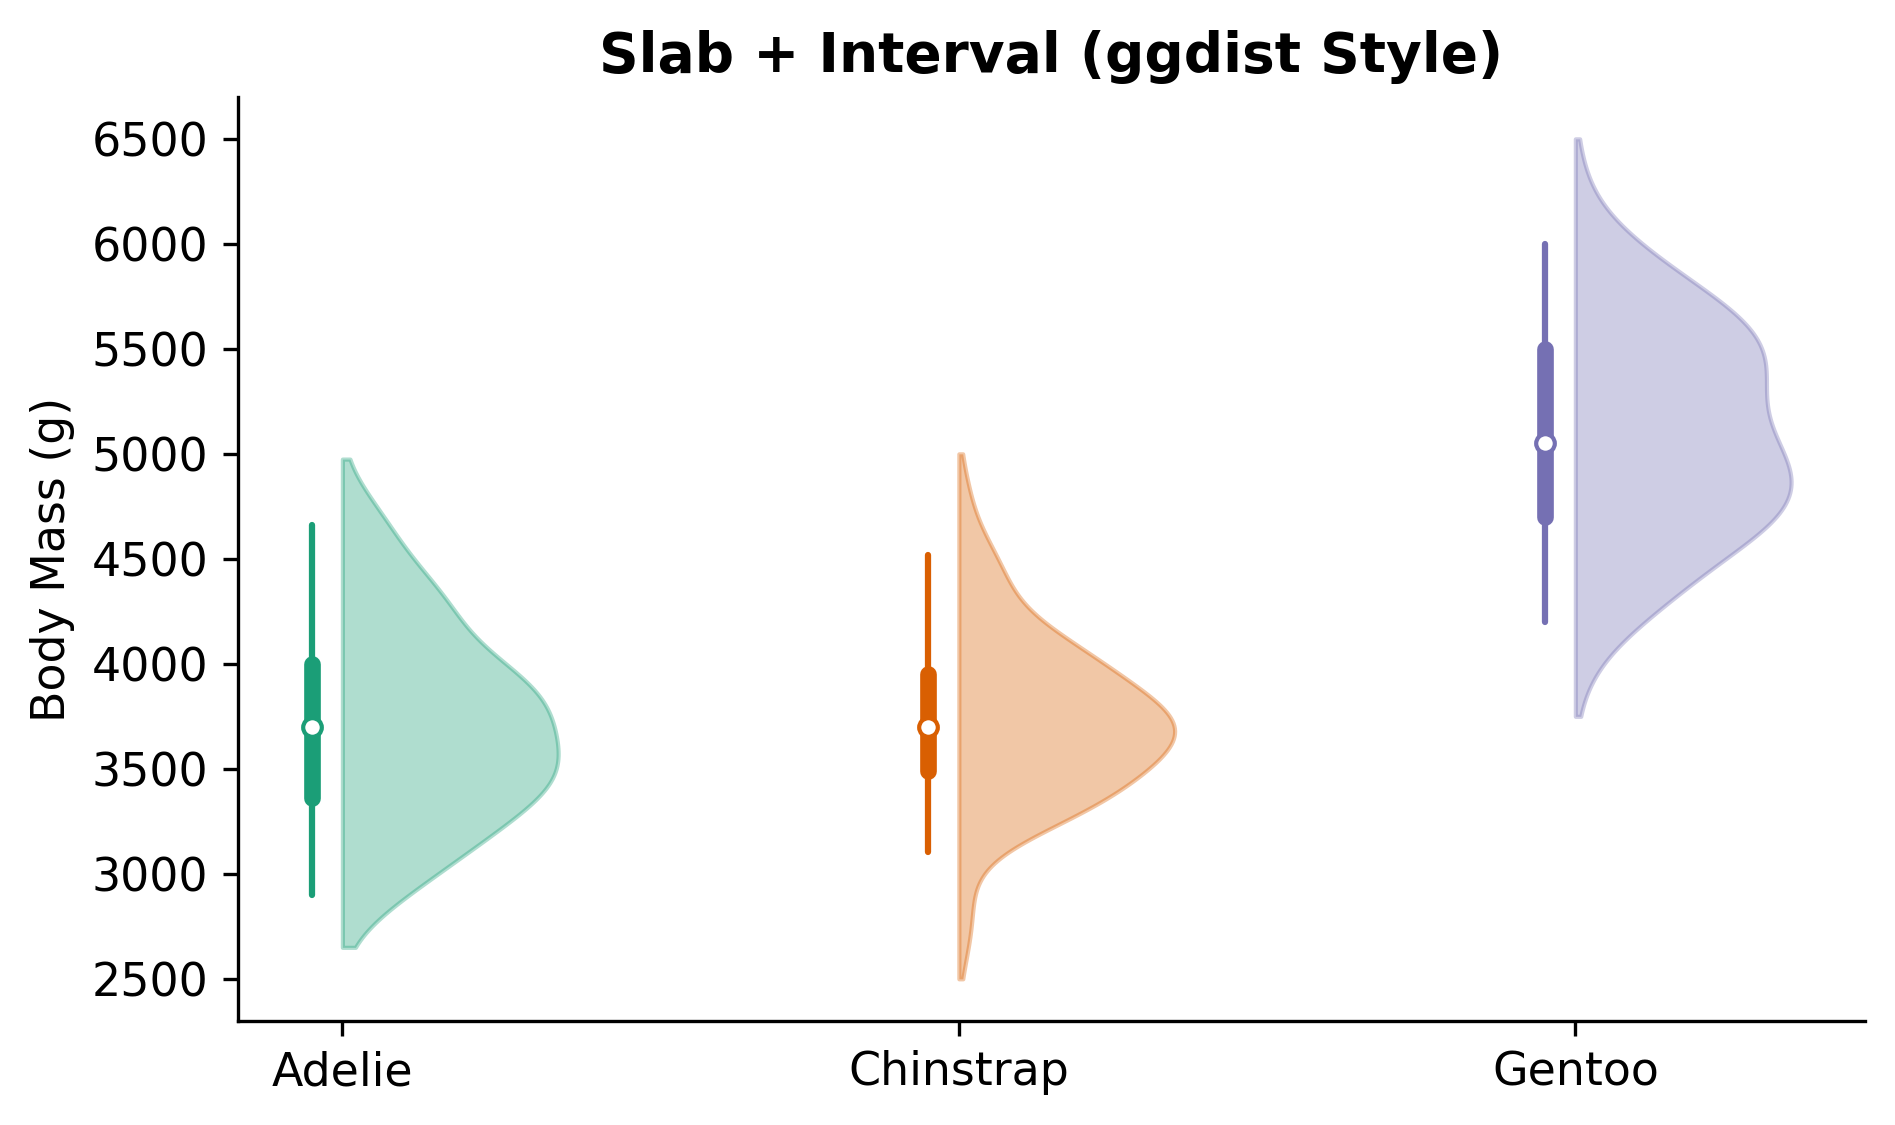
\includegraphics[width=\textwidth]{m2_4_slab_interval.png}
\begin{alertblock}{Pro-Tip}
    \scriptsize \texttt{.width=c(0.5,0.95)} draws two nested intervals: thick bar for 50\% (IQR) and thin bar for 95\%. \texttt{median\_qi} uses median + quantile interval.
\end{alertblock}
\end{column}
\end{columns}
\end{frame}

% ── 98 ──
\begin{frame}[fragile]{Slab + Interval --- \Python}\smark{98/300}
\begin{columns}[T]
\begin{column}{0.55\textwidth}
\begin{lstlisting}[style=Pystyle]
# Manual construction in matplotlib
from scipy.stats import gaussian_kde

for i, (sp, c) in enumerate(
    zip(species_list, colors)):
    data = pen[pen.species==sp]\
        ["body_mass_g"].values
    kde = gaussian_kde(data)
    xs = np.linspace(
        data.min()-200,
        data.max()+200, 200)
    dens = kde(xs)/kde(xs).max()*0.35
    # Slab
    ax.fill_betweenx(xs, i, i+dens,
        color=c, alpha=0.35)
    # Interval: thick=IQR, thin=95%
    q25,med,q75 = np.percentile(
        data, [25,50,75])
    q025,q975 = np.percentile(
        data, [2.5,97.5])
    ax.plot([i,i],[q025,q975],
        color=c, lw=1.5)
    ax.plot([i,i],[q25,q75],
        color=c, lw=4)
\end{lstlisting}
\end{column}
\begin{column}{0.42\textwidth}
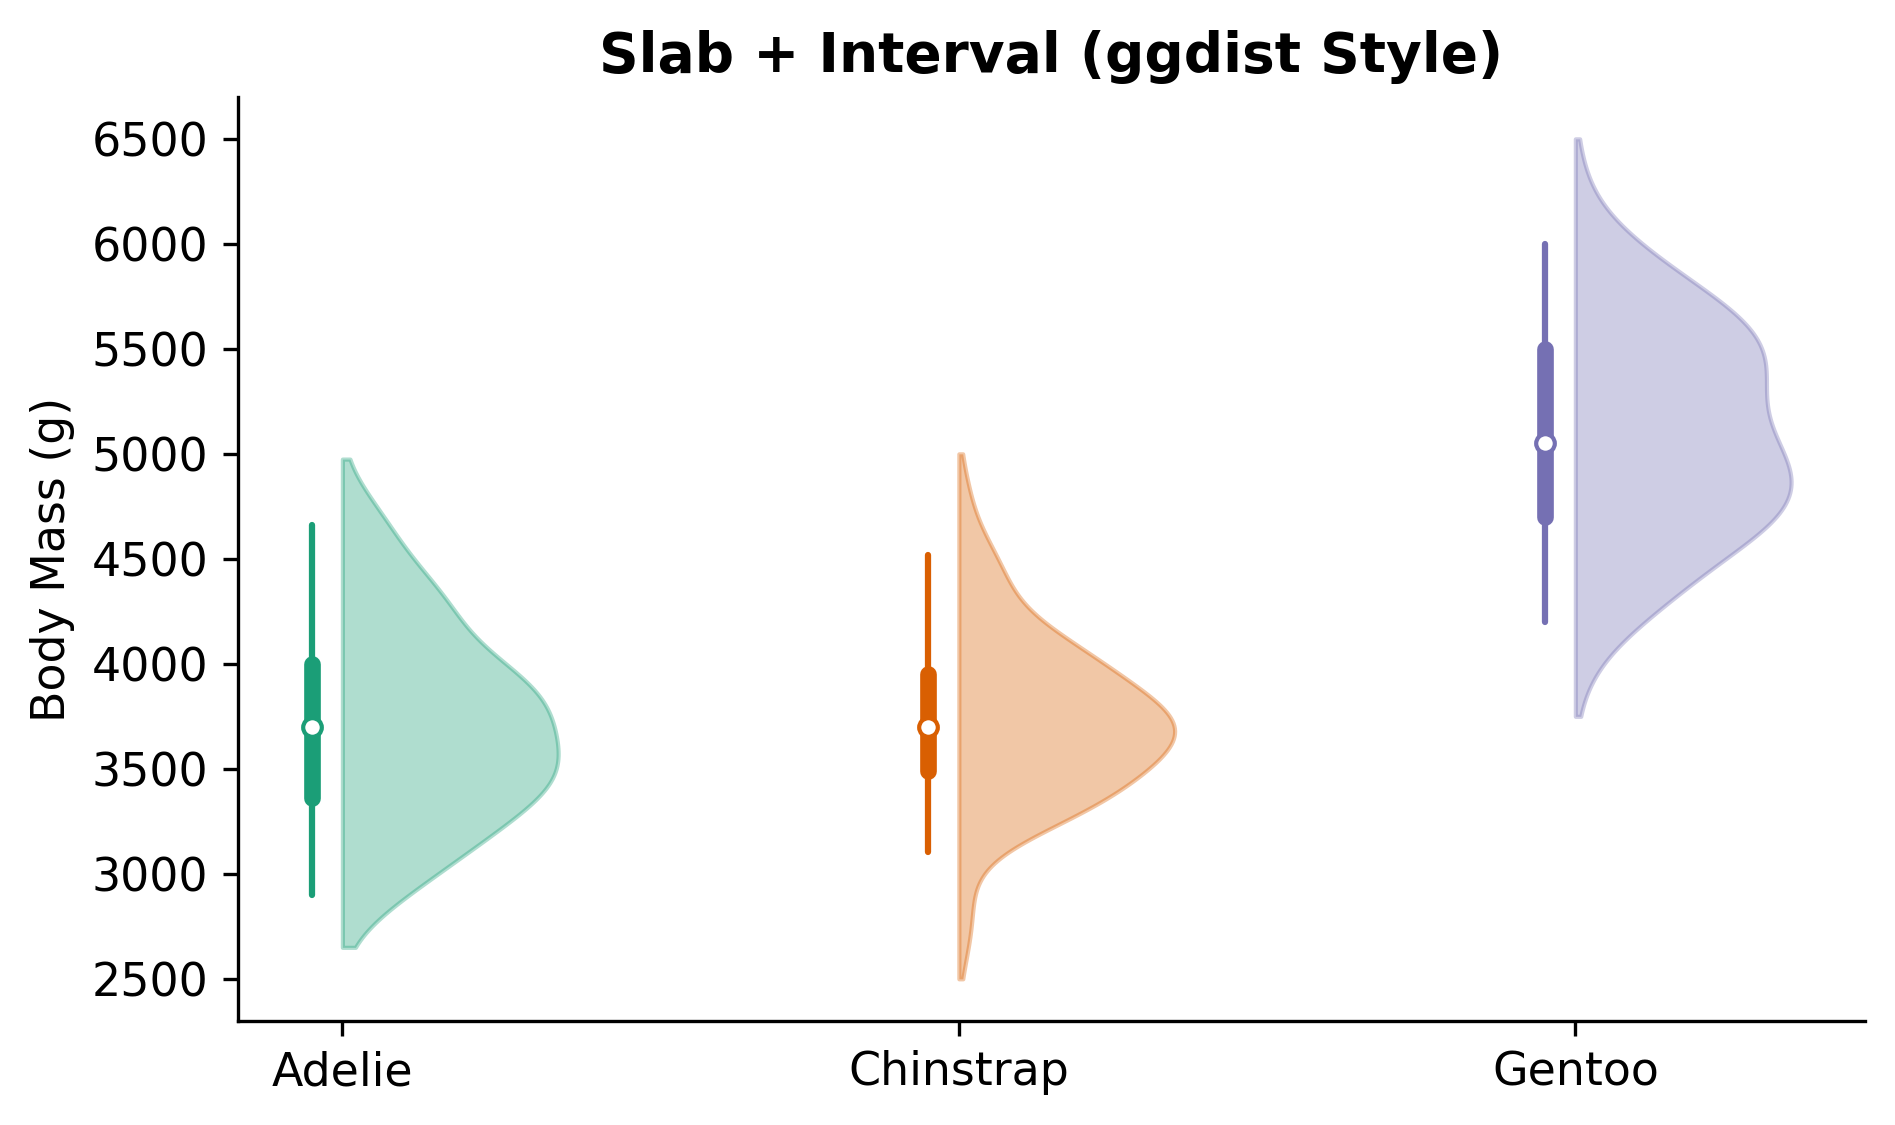
\includegraphics[width=\textwidth]{m2_4_slab_interval.png}
\begin{exampleblock}{Data Insight}
    \scriptsize Python has no \texttt{ggdist} equivalent yet. Build manually with \texttt{fill\_betweenx()} for the slab and \texttt{ax.plot()} for the interval bars. Wrap in a helper function for reuse.
\end{exampleblock}
\end{column}
\end{columns}
\end{frame}

% ── 99 ──
\begin{frame}{Ribbon Bands for Time Series}
\smark{99/300}
\centering
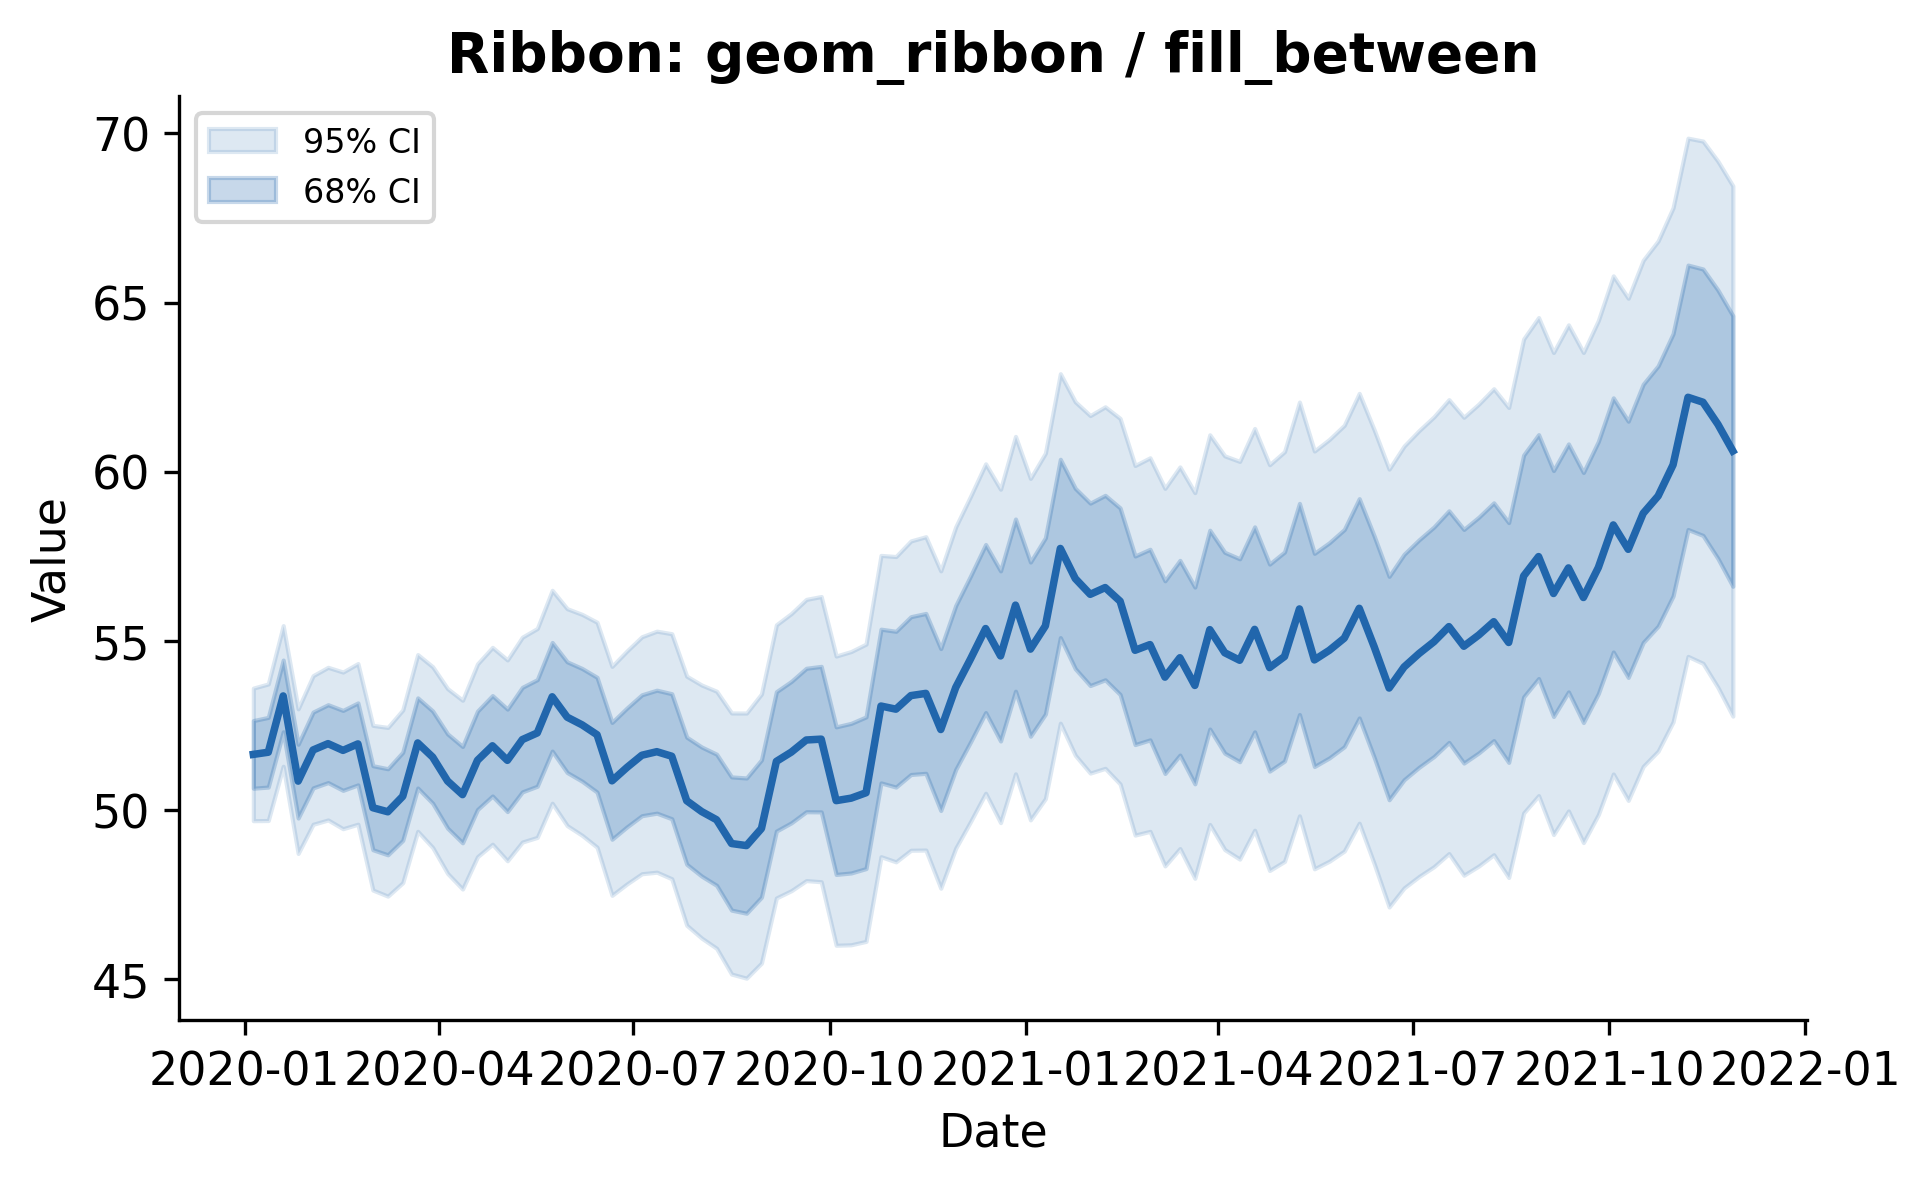
\includegraphics[width=0.78\textwidth]{m2_4_ribbon.png}

\vspace{0.2cm}
\begin{columns}[T]
\begin{column}{0.48\textwidth}
\begin{itemize}
    \item \texttt{geom\_ribbon()} fills between \texttt{ymin} and \texttt{ymax}
    \item Typically 68\% (1 SE) and 95\% (2 SE) bands nested
    \item Used for model predictions, forecast uncertainty, rolling CIs
\end{itemize}
\end{column}
\begin{column}{0.48\textwidth}
\begin{alertblock}{Pro-Tip}
    \scriptsize Layer darker (narrower) band on top of lighter (wider) band. Use \texttt{alpha=0.15} for the 95\% and \texttt{alpha=0.30} for the 68\% band.
\end{alertblock}
\end{column}
\end{columns}
\end{frame}

% ── 100 ──
\begin{frame}[fragile]{Ribbon --- Code}\smark{100/300}
\begin{columns}[T]
\begin{column}{0.48\textwidth}
\begin{lstlisting}[style=Rstyle]
ggplot(df, aes(date, value)) +
  geom_ribbon(
    aes(ymin = value - 1.96*se,
        ymax = value + 1.96*se),
    alpha = 0.15, fill="#2166AC")+
  geom_ribbon(
    aes(ymin = value - se,
        ymax = value + se),
    alpha = 0.25, fill="#2166AC")+
  geom_line(color="#2166AC",
    linewidth = 1) +
  theme_minimal()
\end{lstlisting}
\end{column}
\begin{column}{0.48\textwidth}
\begin{lstlisting}[style=Pystyle]
ax.fill_between(dates,
    y - 1.96*se, y + 1.96*se,
    alpha=0.15, color="#2166AC",
    label="95% CI")
ax.fill_between(dates,
    y - se, y + se,
    alpha=0.25, color="#2166AC",
    label="68% CI")
ax.plot(dates, y,
    color="#2166AC", linewidth=1.5)
\end{lstlisting}
\vspace{0.1cm}
\begin{exampleblock}{Data Insight}
    \scriptsize Ribbon order matters: wide (95\%) first, narrow (68\%) on top. Both use the same color; alpha transparency creates the layered effect.
\end{exampleblock}
\end{column}
\end{columns}
\end{frame}

% ── 101 ──
\begin{frame}{Fan Charts: Gradient Intervals for Forecasts}
\smark{101/300}
\centering
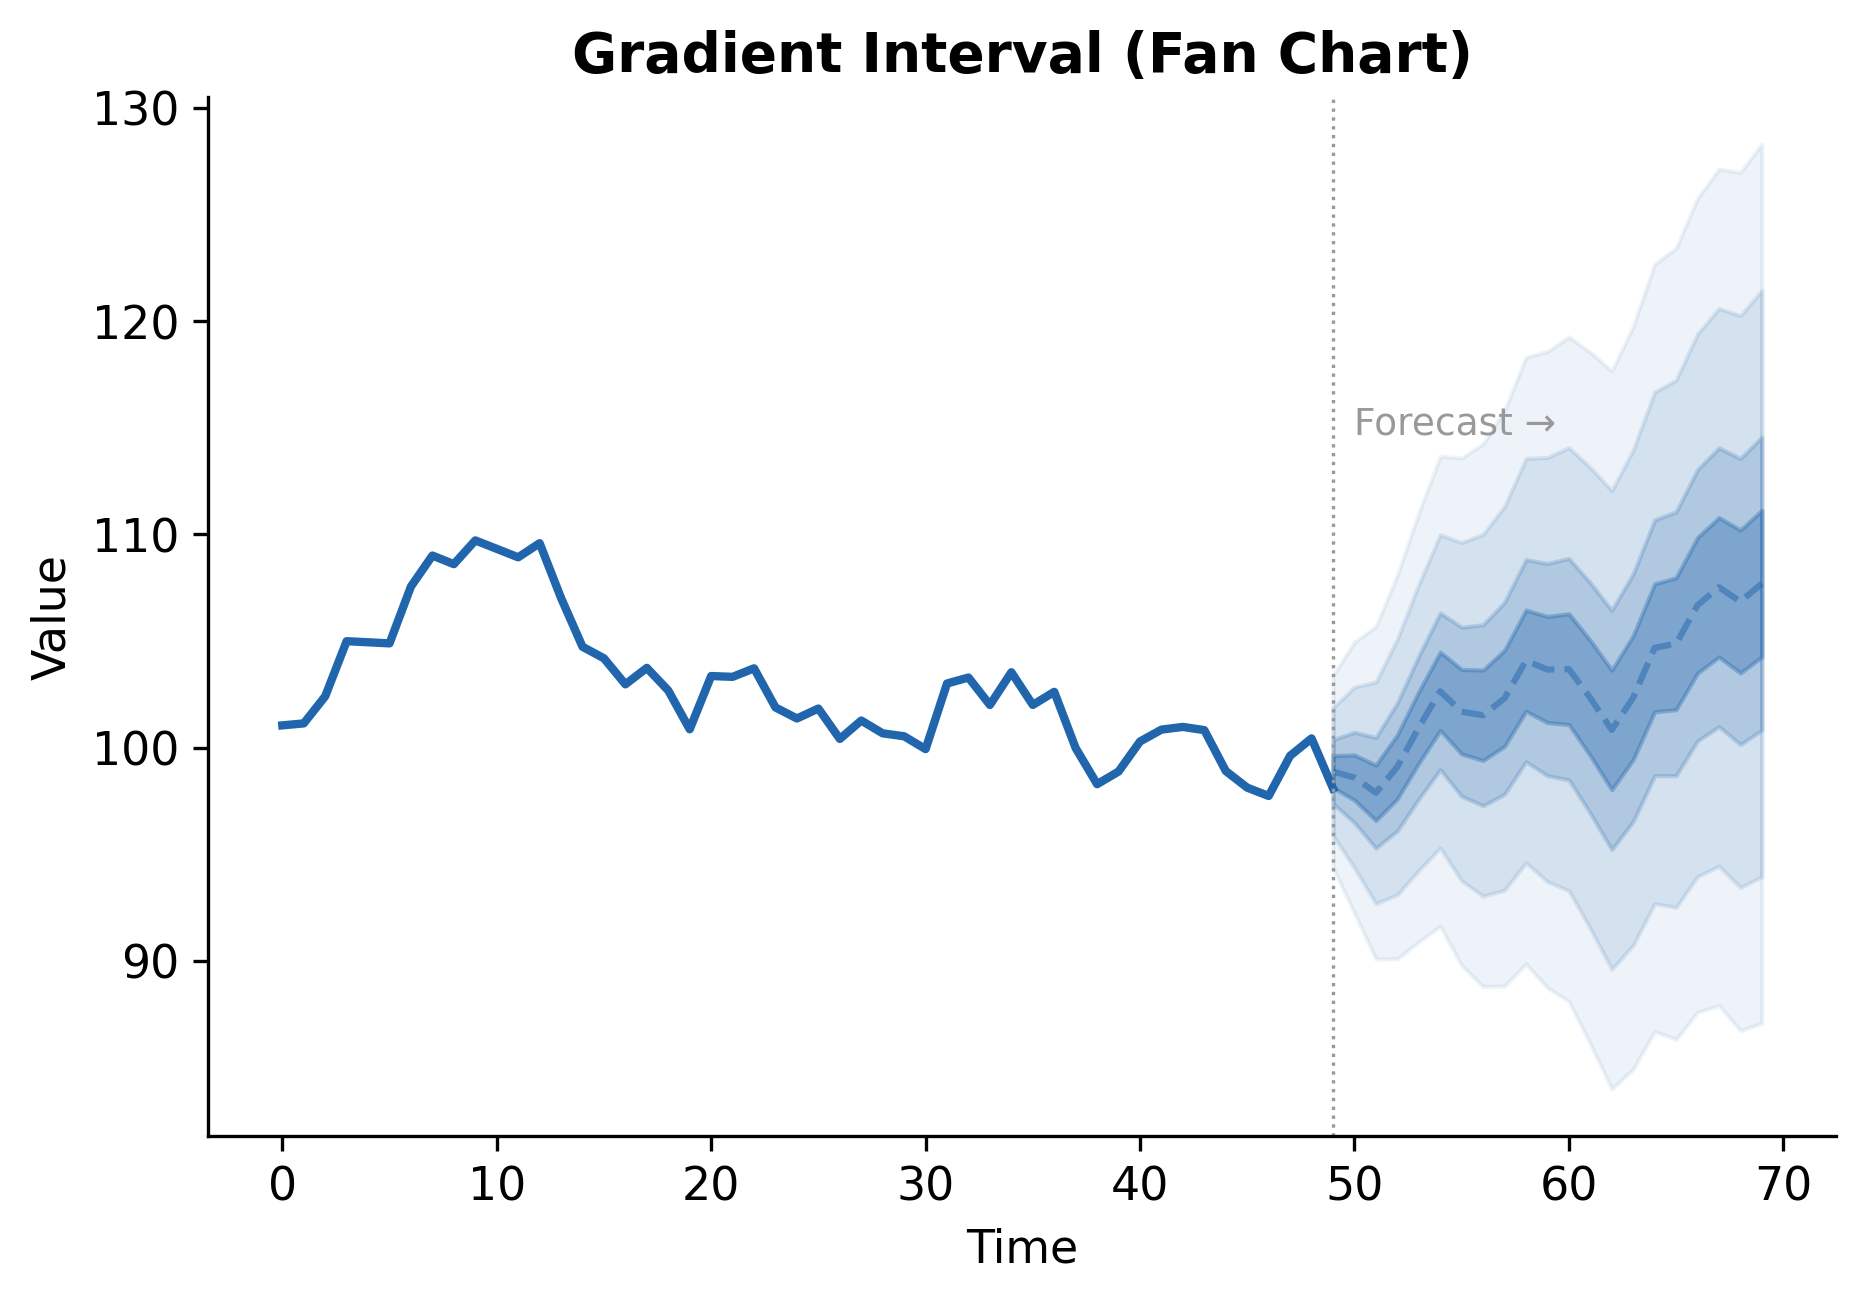
\includegraphics[width=0.78\textwidth]{m2_4_gradient_ci.png}

\vspace{0.2cm}
\begin{columns}[T]
\begin{column}{0.48\textwidth}
\begin{itemize}
    \item Multiple nested ribbons with decreasing alpha
    \item Uncertainty \textbf{grows} with forecast horizon
    \item Used by central banks (Bank of England), weather services
    \item The ``eye of the hurricane'' visual
\end{itemize}
\end{column}
\begin{column}{0.48\textwidth}
\begin{exampleblock}{Data Insight}
    \scriptsize The fan shape makes uncertainty's temporal structure visceral: the near future is well-constrained; the distant future is wide open. No error bar can convey this as effectively.
\end{exampleblock}
\end{column}
\end{columns}
\end{frame}

% ── 102 ──
\begin{frame}[fragile]{Fan Chart --- Code}\smark{102/300}
\begin{columns}[T]
\begin{column}{0.48\textwidth}
\begin{lstlisting}[style=Rstyle]
# Multiple nested ribbons
alphas <- c(0.08, 0.12, 0.20, 0.35)
widths <- c(3, 2, 1, 0.5) # x SE

for (i in seq_along(alphas)) {
  p <- p + geom_ribbon(
    aes(ymin = fit - widths[i]*se,
        ymax = fit + widths[i]*se),
    alpha = alphas[i],
    fill = "#2166AC")
}
p + geom_line(aes(y=fit),
    color="#2166AC")
\end{lstlisting}
\end{column}
\begin{column}{0.48\textwidth}
\begin{lstlisting}[style=Pystyle]
for alpha_val, mult in [
    (0.08, 3.0), (0.12, 2.0),
    (0.20, 1.0), (0.35, 0.5)]:
    spread = mult * np.sqrt(
        np.arange(1, n_fut+1)) * s
    ax.fill_between(x_fut,
        y_hat - spread,
        y_hat + spread,
        alpha=alpha_val,
        color="#2166AC")
ax.plot(x_fut, y_hat,
    color="#2166AC", linewidth=1.5)
\end{lstlisting}
\vspace{0.1cm}
\begin{alertblock}{Pro-Tip}
    \scriptsize For fan charts, compute $\text{spread} \propto \sqrt{h}$ where $h$ = forecast horizon. This follows from the random-walk variance formula $\text{Var}(X_{t+h}) = h \sigma^2$.
\end{alertblock}
\end{column}
\end{columns}
\end{frame}

% ── 103 ──
\begin{frame}{Forest Plots: Meta-Analysis and Multi-Study}
\smark{103/300}
\centering
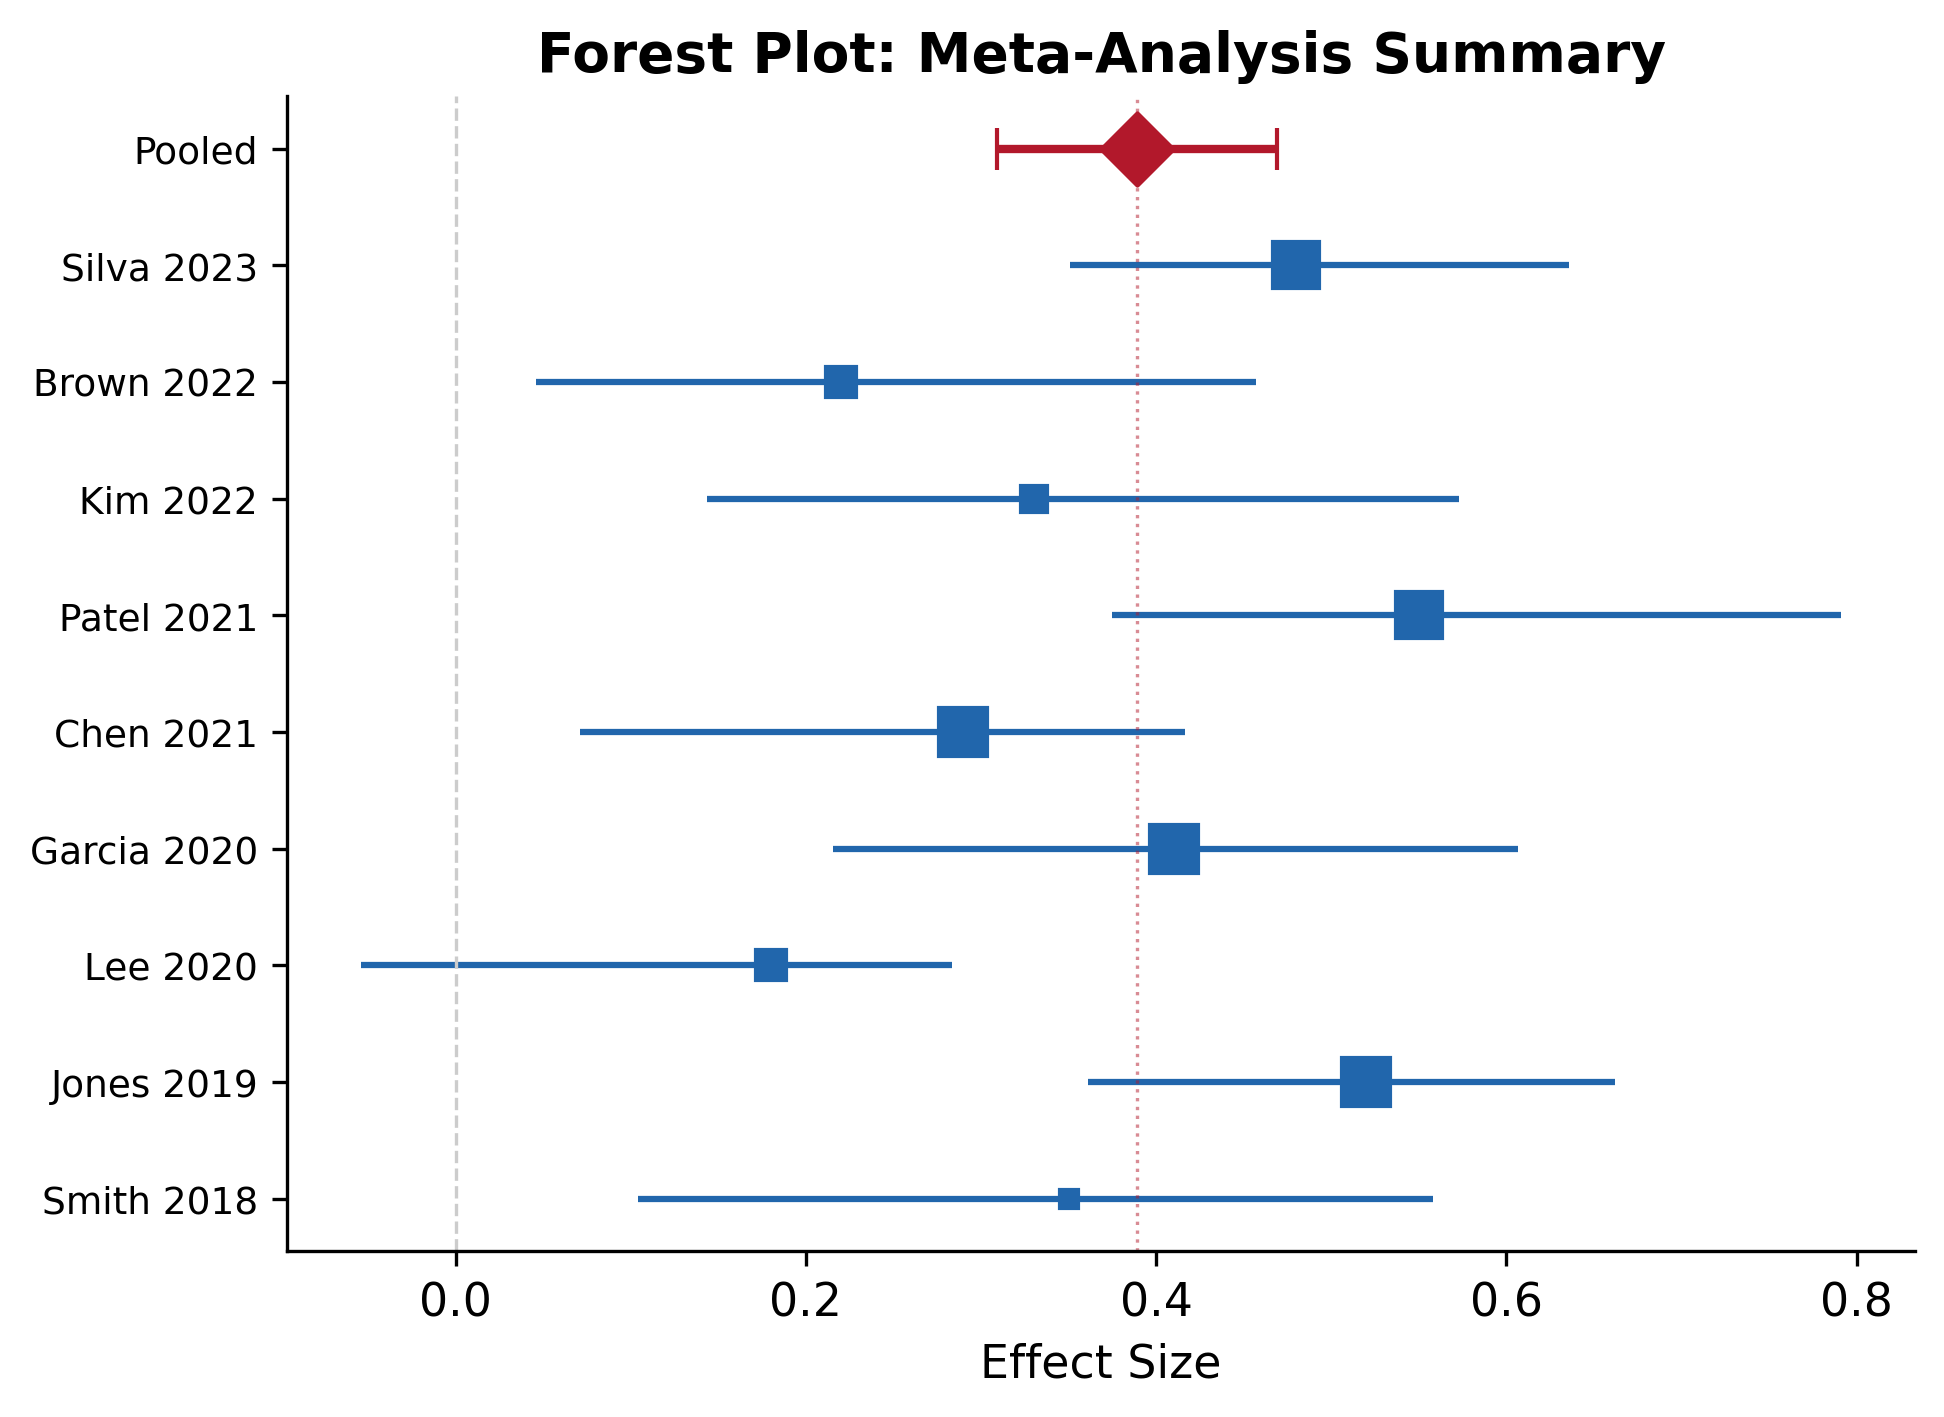
\includegraphics[width=0.68\textwidth]{m2_4_forest_plot.png}

\vspace{0.2cm}
\begin{columns}[T]
\begin{column}{0.48\textwidth}
\begin{itemize}
    \item One row per study (or subgroup)
    \item Square = point estimate (size $\propto$ weight)
    \item Horizontal line = 95\% CI
    \item Diamond = pooled estimate
    \item Vertical dashed line at null effect (0 or 1)
\end{itemize}
\end{column}
\begin{column}{0.48\textwidth}
\begin{exampleblock}{Data Insight}
    \scriptsize Forest plots make heterogeneity visible: if CIs overlap heavily, studies agree; if they don't, the pooled estimate is questionable. Cochrane reviews require them.
\end{exampleblock}
\end{column}
\end{columns}
\end{frame}

% ── 104 ──
\begin{frame}[fragile]{Forest Plot --- \Rlang}\smark{104/300}
\begin{columns}[T]
\begin{column}{0.55\textwidth}
\begin{lstlisting}[style=Rstyle]
library(meta)
# From meta-analysis object
forest(meta_obj,
  col.square = "#2166AC",
  col.diamond = "#B2182B")

# Manual with ggplot2
ggplot(studies_df,
  aes(estimate,
      fct_reorder(study,
                  estimate))) +
  geom_pointrange(
    aes(xmin=ci_lo, xmax=ci_hi),
    size = 0.6) +
  geom_vline(xintercept = 0,
    linetype="dashed") +
  labs(x="Effect Size", y=NULL)+
  theme_minimal()
\end{lstlisting}
\end{column}
\begin{column}{0.42\textwidth}
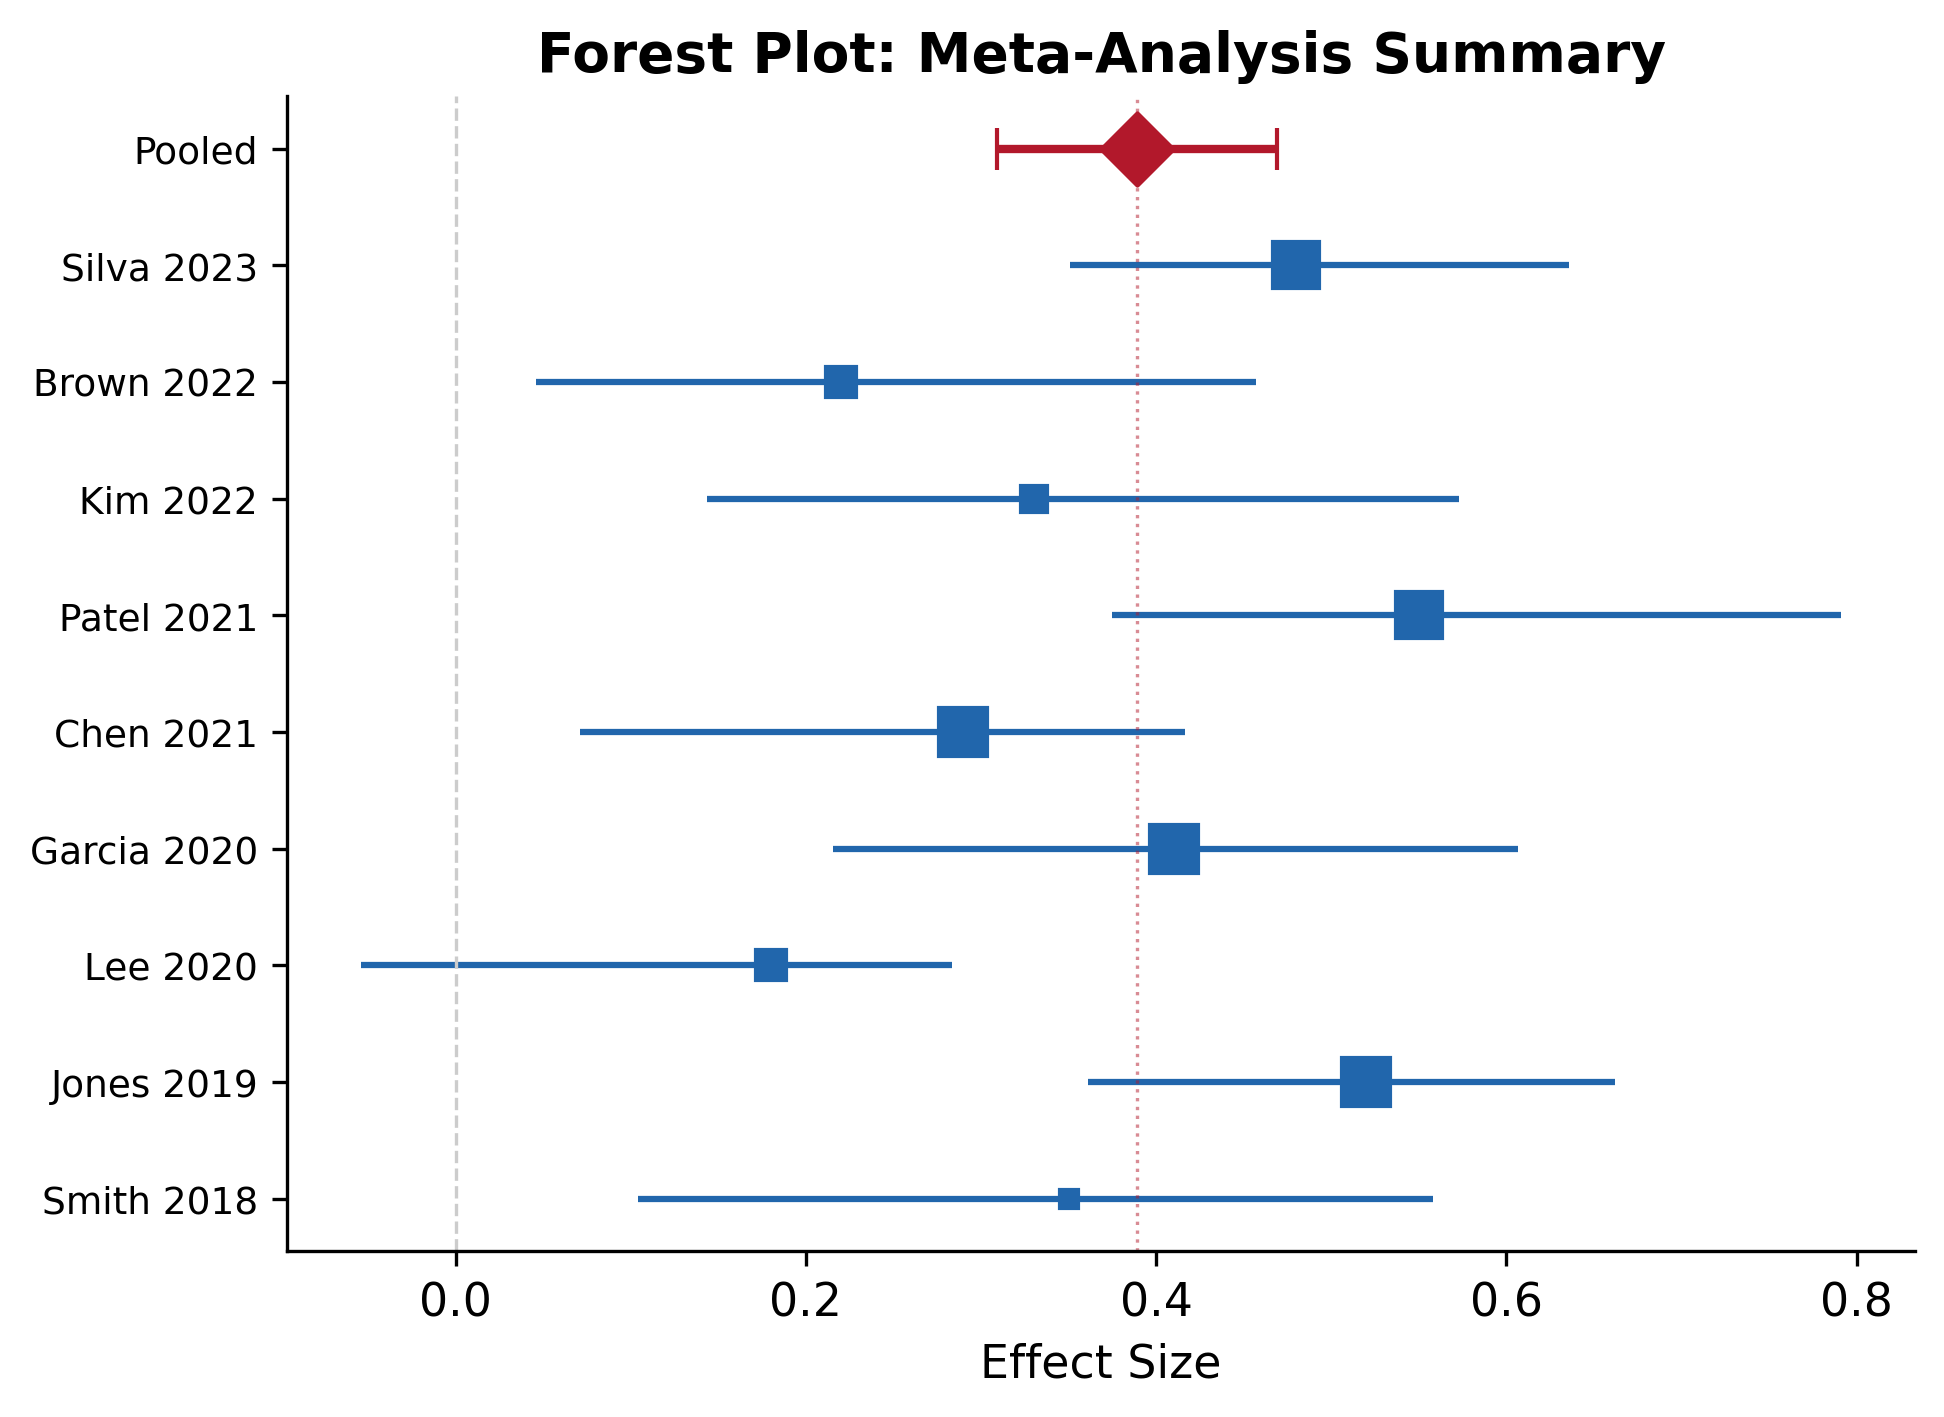
\includegraphics[width=\textwidth]{m2_4_forest_plot.png}
\begin{alertblock}{Pro-Tip}
    \scriptsize The \texttt{meta} and \texttt{metafor} packages produce publication-ready forest plots. For custom styling, extract the data and plot with ggplot2.
\end{alertblock}
\end{column}
\end{columns}
\end{frame}

% ── 105 ──
\begin{frame}[fragile]{Forest Plot --- \Python}\smark{105/300}
\begin{columns}[T]
\begin{column}{0.55\textwidth}
\begin{lstlisting}[style=Pystyle]
fig, ax = plt.subplots()

for i, row in studies.iterrows():
    ax.errorbar(row["effect"], i,
        xerr=[[row["effect"]-row["lo"]],
              [row["hi"]-row["effect"]]],
        fmt="s", color="#2166AC",
        markersize=row["weight"]*0.8,
        linewidth=1.5, capsize=0)

# Pooled diamond
ax.scatter(pooled, len(studies),
    marker="D", s=150,
    color="#B2182B", zorder=5)

ax.axvline(0, linestyle="--",
    color="#CCC")
ax.set_yticks(range(len(studies)+1))
ax.set_yticklabels(
    list(studies["name"])+["Pooled"])
\end{lstlisting}
\end{column}
\begin{column}{0.42\textwidth}
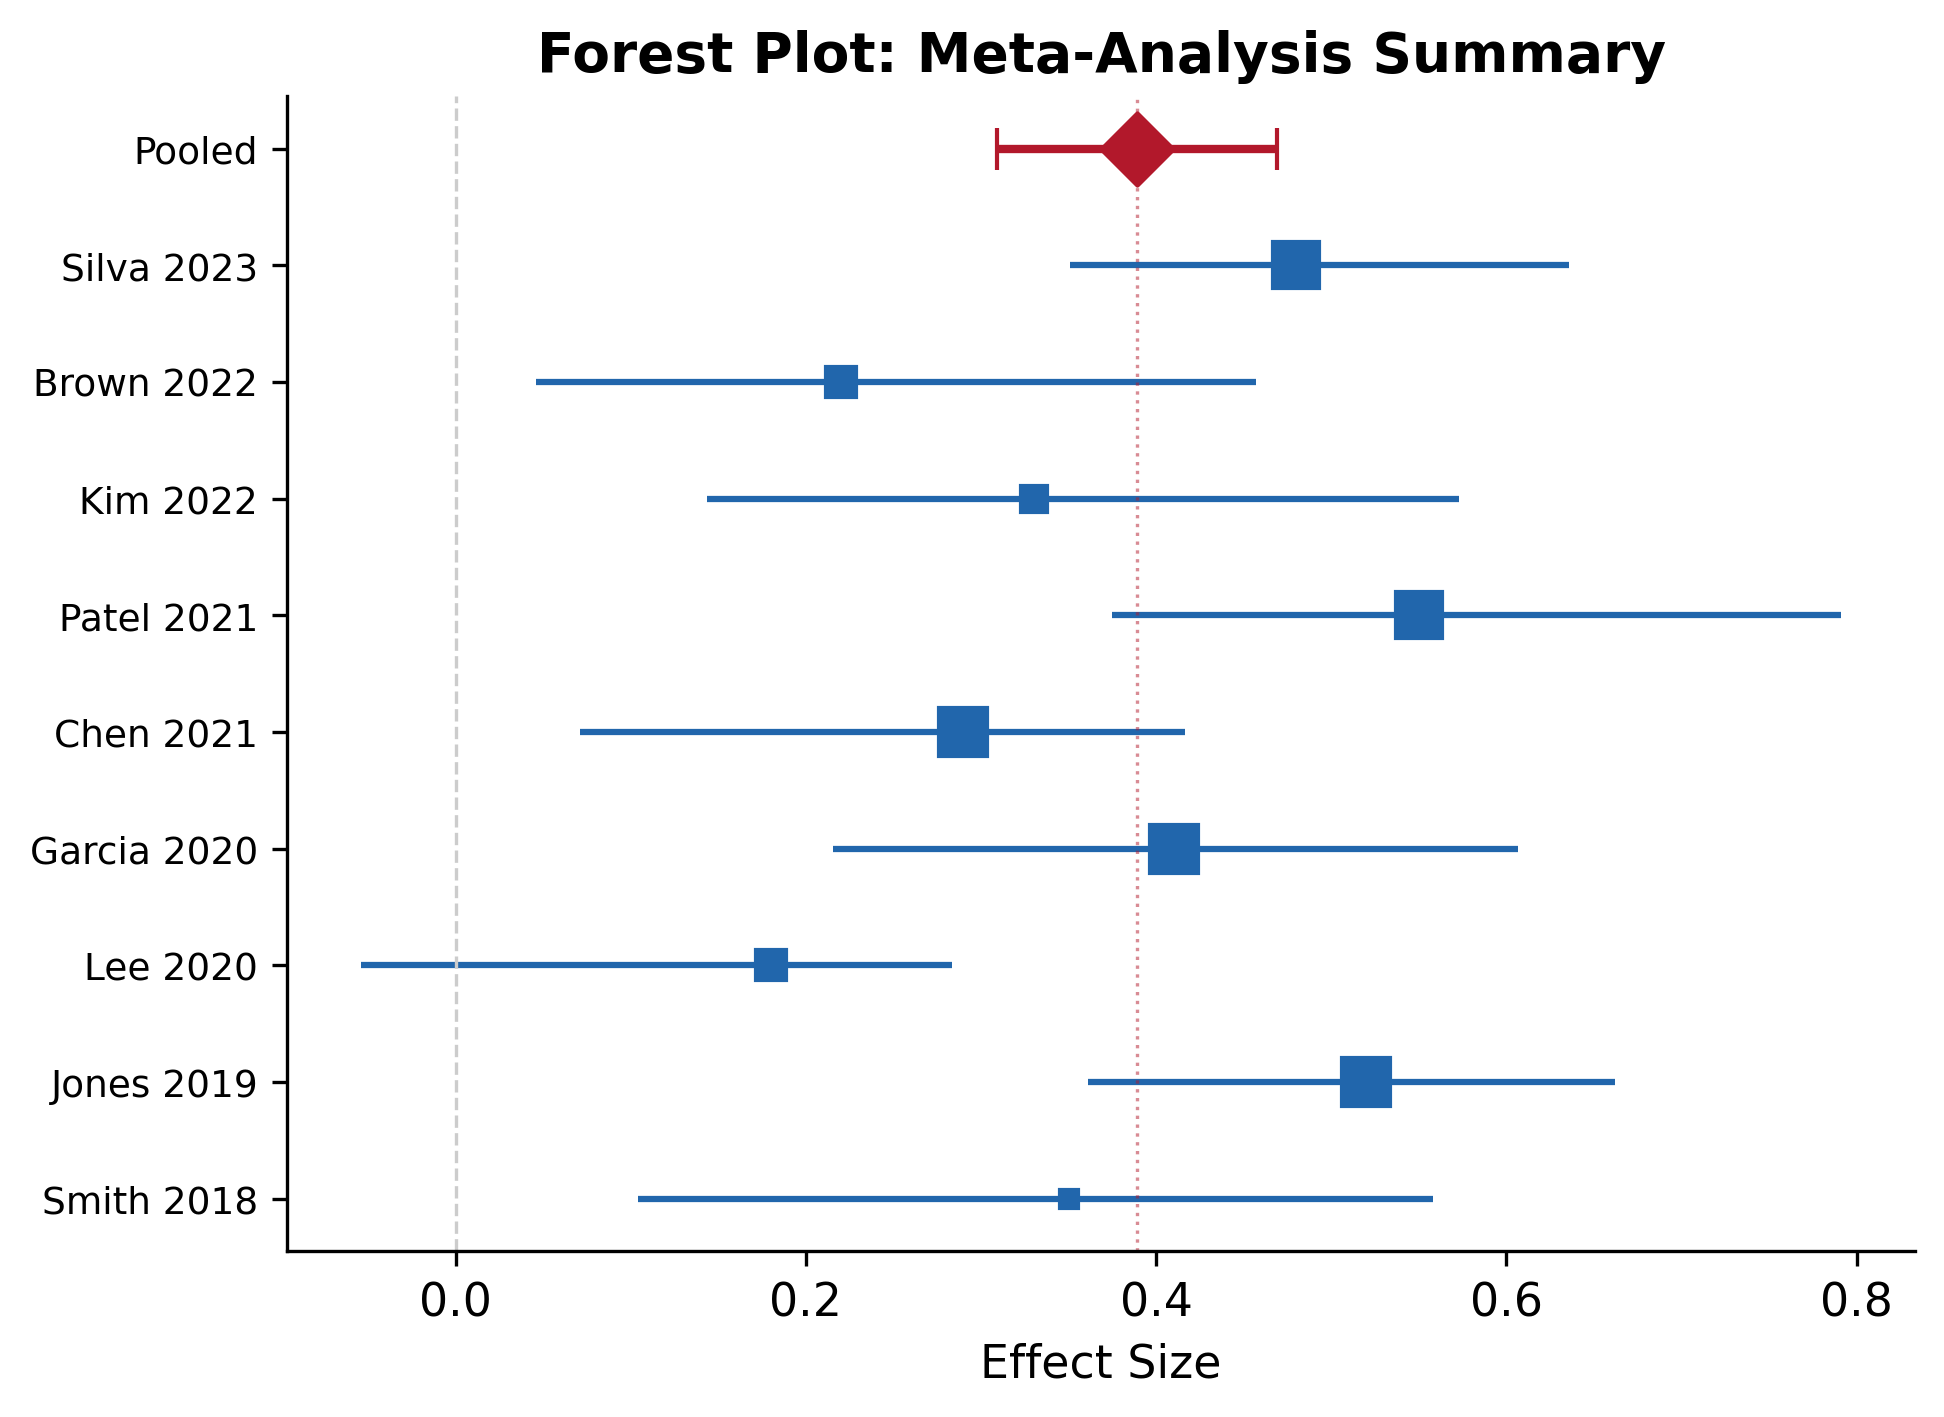
\includegraphics[width=\textwidth]{m2_4_forest_plot.png}
\begin{exampleblock}{Data Insight}
    \scriptsize Python has no built-in forest plot. \texttt{ax.errorbar()} with square markers (\texttt{fmt="s"}) and variable \texttt{markersize} recreates it. The \texttt{forestplot} PyPI package provides a higher-level API.
\end{exampleblock}
\end{column}
\end{columns}
\end{frame}

% ── 106 ──
\begin{frame}{Bayesian Posteriors and HDI}
\smark{106/300}
\centering
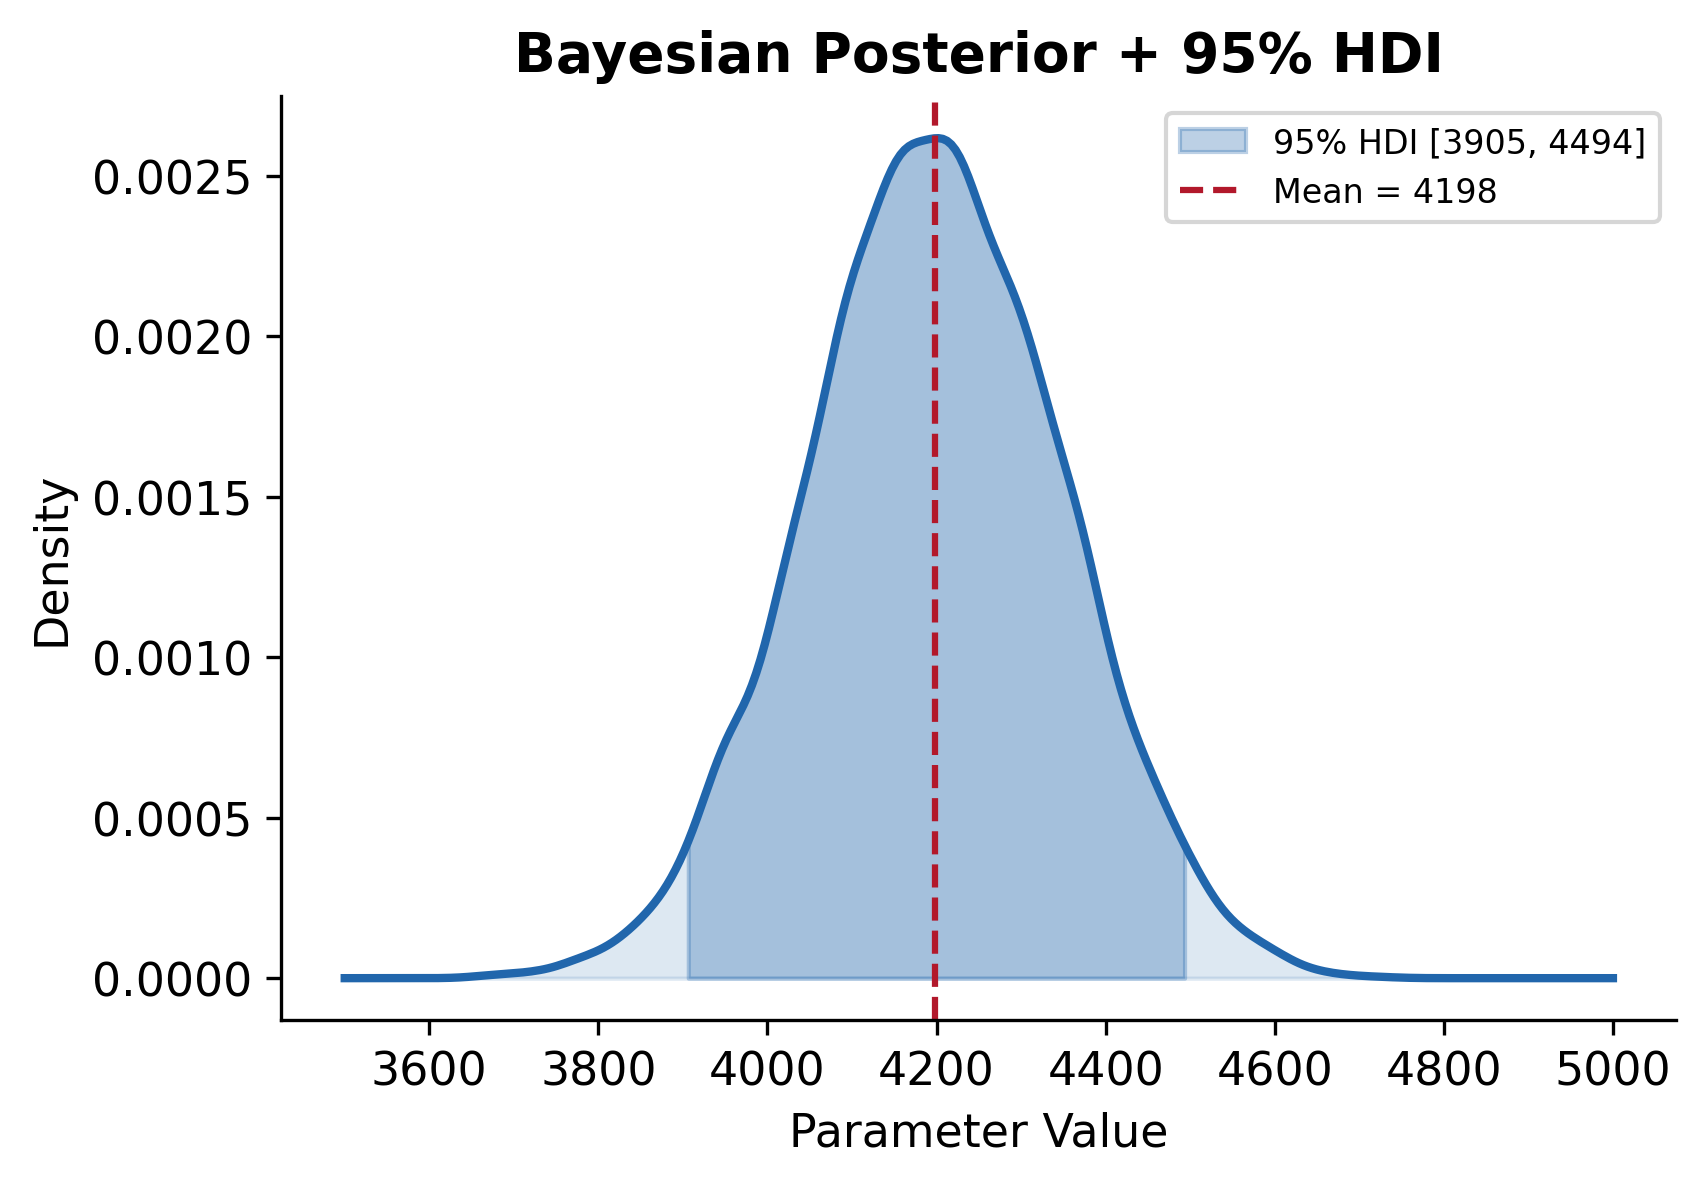
\includegraphics[width=0.68\textwidth]{m2_4_bayesian_hdi.png}

\vspace{0.2cm}
\begin{columns}[T]
\begin{column}{0.48\textwidth}
\begin{itemize}
    \item \textbf{Posterior}: probability distribution of the parameter \emph{given the data}
    \item \textbf{HDI}: Highest Density Interval --- narrowest interval containing 95\% of the posterior mass
    \item HDI $\neq$ equal-tailed CI (differs for skewed posteriors)
\end{itemize}
\end{column}
\begin{column}{0.48\textwidth}
\begin{alertblock}{Pro-Tip}
    \scriptsize R: \texttt{bayesplot::mcmc\_areas()} or \texttt{ggdist::stat\_halfeye()} on posterior draws. Python: \texttt{arviz.plot\_posterior()} from the ArviZ library.
\end{alertblock}
\end{column}
\end{columns}
\end{frame}

% ── 107 ──
\begin{frame}[fragile]{Bayesian Posterior --- Code}\smark{107/300}
\begin{columns}[T]
\begin{column}{0.48\textwidth}
\begin{lstlisting}[style=Rstyle]
library(bayesplot)

# From brms/rstanarm posterior
mcmc_areas(posterior_draws,
  pars = c("bill_length_mm"),
  prob = 0.95,   # HDI
  prob_outer = 1)

# ggdist on raw draws
ggplot(draws_df,
  aes(x = beta)) +
  stat_halfeye(
    .width = c(0.66, 0.95),
    fill = "#2166AC",
    alpha = 0.4) +
  geom_vline(xintercept = 0,
    linetype="dashed",
    color="#B2182B")
\end{lstlisting}
\end{column}
\begin{column}{0.48\textwidth}
\begin{lstlisting}[style=Pystyle]
import arviz as az

# From PyMC / Stan trace
az.plot_posterior(trace,
    var_names=["beta"],
    hdi_prob=0.95)

# Manual
posterior = trace["beta"]
ax.hist(posterior, bins=50,
    density=True, alpha=0.3,
    color="#2166AC")
hdi = az.hdi(posterior,
    hdi_prob=0.95)
ax.axvspan(hdi[0], hdi[1],
    alpha=0.15, color="#2166AC")
ax.axvline(0, linestyle="--",
    color="#B2182B")
\end{lstlisting}
\end{column}
\end{columns}
\end{frame}

% ── 108 ──
\begin{frame}{Hypothetical Outcome Plots (HOPs)}
\smark{108/300}
\centering
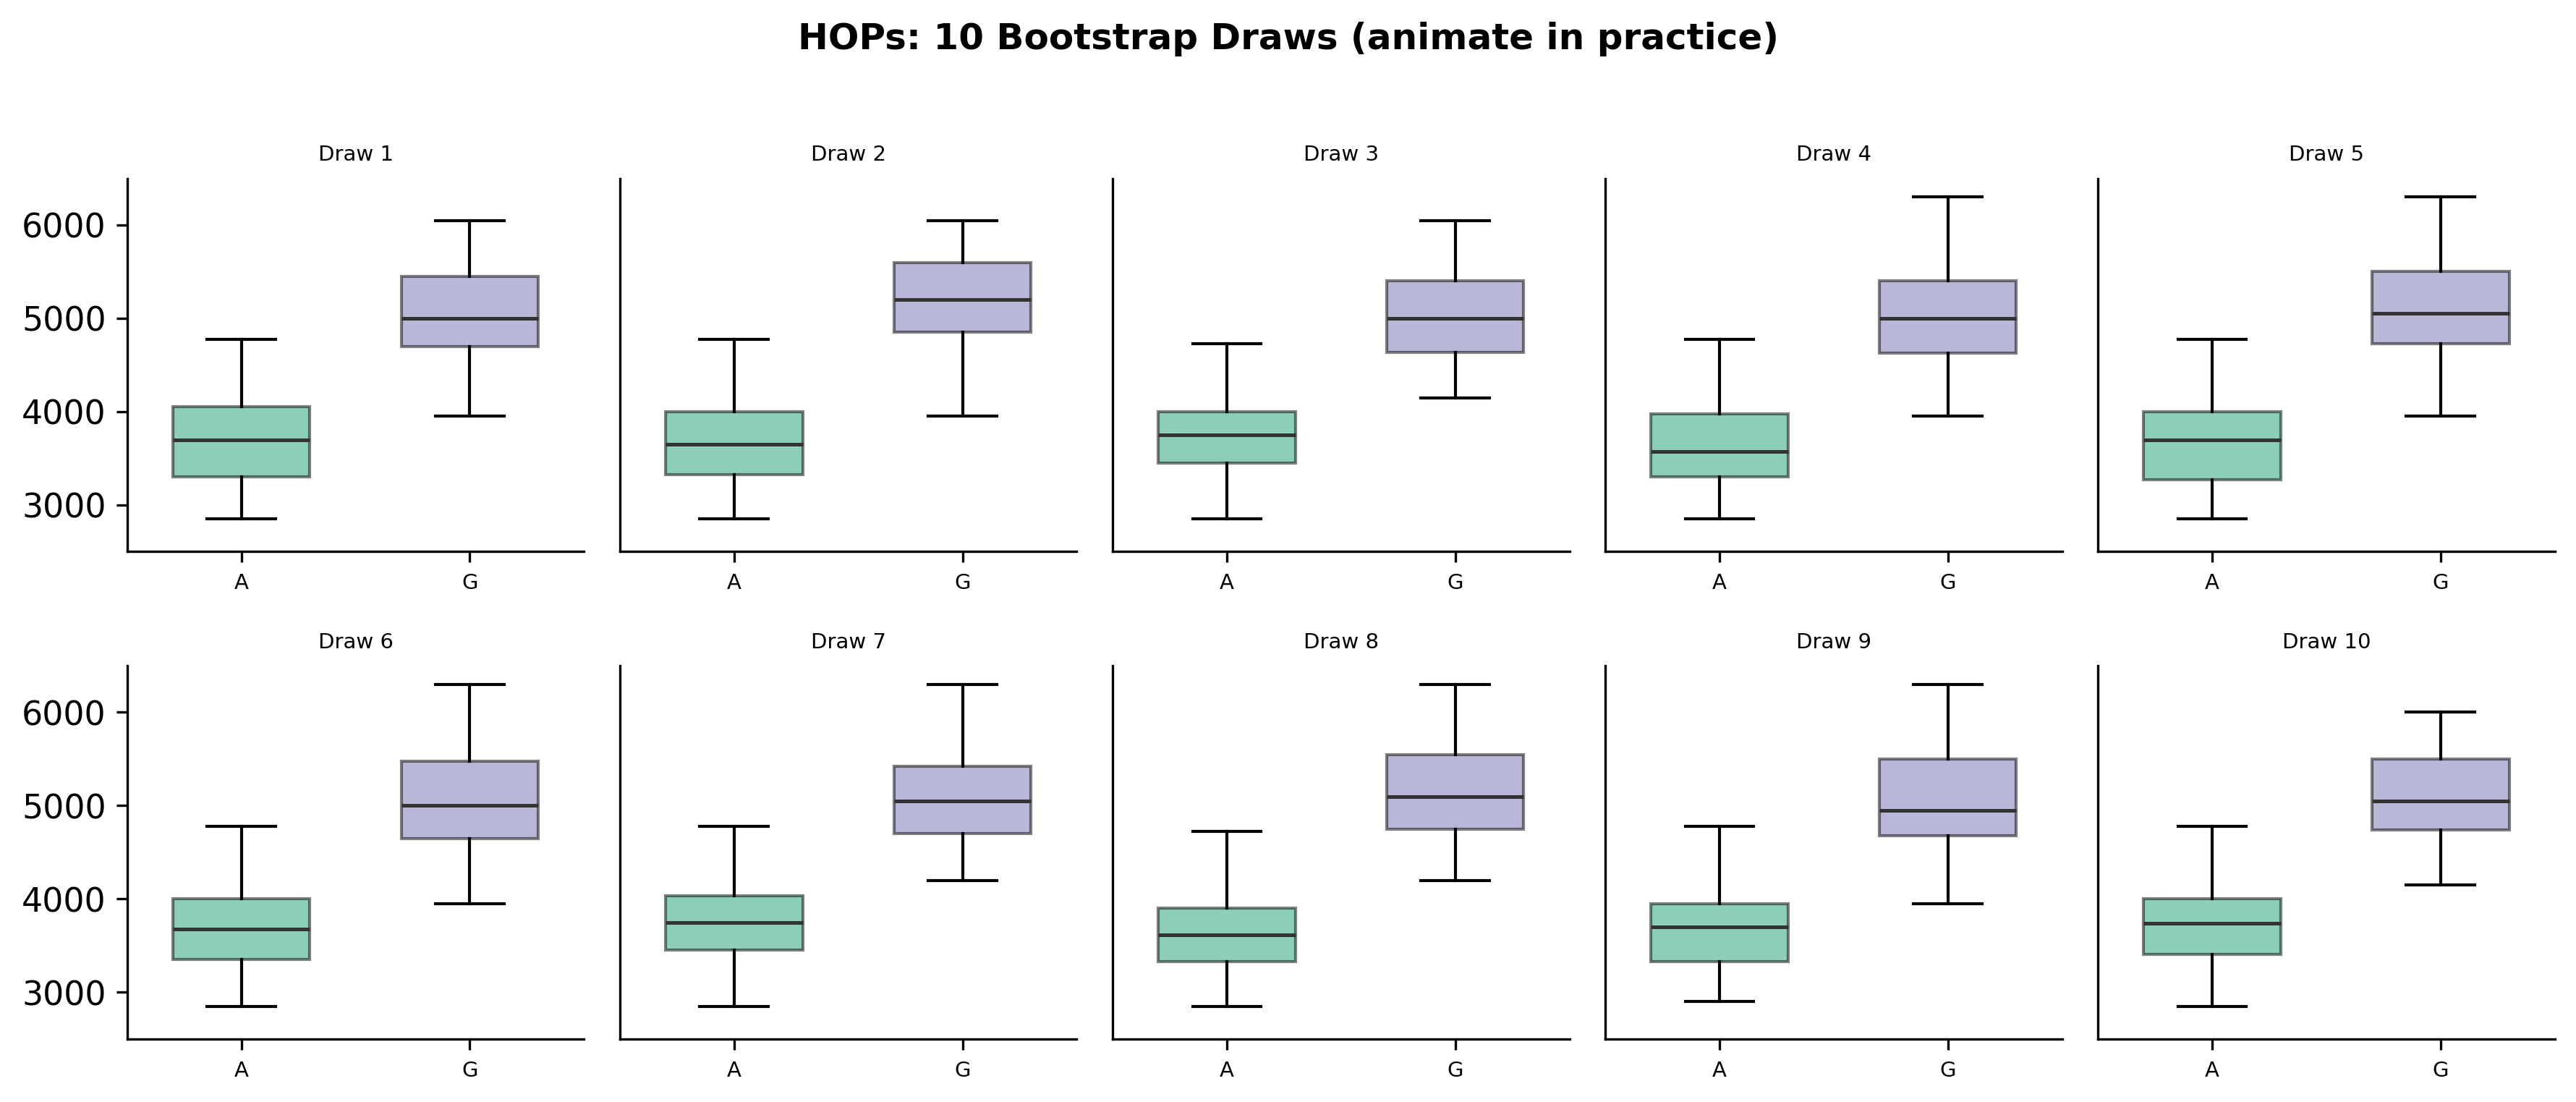
\includegraphics[width=0.85\textwidth]{m2_4_hops.png}

\vspace{0.2cm}
\begin{columns}[T]
\begin{column}{0.48\textwidth}
\begin{itemize}
    \item \textbf{Animated} sequence of bootstrap draws
    \item Each frame shows one plausible dataset
    \item The viewer perceives the \textbf{frequency of outcomes} directly
    \item Hullman et al.\ (2015): HOPs improve uncertainty judgment
\end{itemize}
\end{column}
\begin{column}{0.48\textwidth}
\begin{exampleblock}{Data Insight}
    \scriptsize Static version shown here (10 frames). In practice, animate at 2--5 fps. Each ``flicker'' between frames encodes one unit of sampling variability --- viewers intuit the spread automatically.
\end{exampleblock}
\end{column}
\end{columns}
\end{frame}

% ── 109 ──
\begin{frame}[fragile]{HOPs --- Code}\smark{109/300}
\begin{columns}[T]
\begin{column}{0.48\textwidth}
\begin{lstlisting}[style=Rstyle]
library(gganimate)

# One frame per bootstrap draw
draws <- map_dfr(1:50, function(i) {
  penguins |>
    slice_sample(prop=1,
      replace=TRUE) |>
    mutate(draw = i)
})

ggplot(draws,
  aes(species, body_mass_g)) +
  geom_boxplot(fill="#2166AC",
    alpha=0.4) +
  transition_states(draw,
    transition_length=1,
    state_length=0.5) +
  labs(title="Draw: {closest_state}")
\end{lstlisting}
\end{column}
\begin{column}{0.48\textwidth}
\begin{lstlisting}[style=Pystyle]
# matplotlib animation
from matplotlib.animation \
    import FuncAnimation

def update(frame):
    ax.clear()
    boot = penguins.sample(
        frac=1, replace=True)
    sns.boxplot(data=boot,
        x="species",
        y="body_mass_g", ax=ax)

anim = FuncAnimation(fig, update,
    frames=50, interval=400)
anim.save("hops.gif",
    writer="pillow")
\end{lstlisting}
\vspace{0.1cm}
\begin{alertblock}{Pro-Tip}
    \scriptsize R: \texttt{gganimate::transition\_states()}. Python: \texttt{matplotlib.animation.FuncAnimation()}. 50 frames at 400\,ms interval $\approx$ 20 seconds.
\end{alertblock}
\end{column}
\end{columns}
\end{frame}

% ── 110 ──
\begin{frame}{Quantile Dot Plots}
\smark{110/300}
\begin{columns}[T]
\begin{column}{0.50\textwidth}
\begin{itemize}
    \item Represent a distribution as $k$ discrete dots at evenly spaced quantiles
    \item Each dot = $1/k$ probability
    \item Viewers can \textbf{count} dots in a region to estimate probability
    \item Kay et al.\ (2016): ``people can read quantile dot plots as well or better than density plots''
\end{itemize}
\end{column}
\begin{column}{0.47\textwidth}
\begin{exampleblock}{Data Insight}
    \scriptsize 20 dots: each = 5\% probability. Count dots above a threshold $\to$ instant probability estimate. This outperforms density plots for lay audiences.
\end{exampleblock}
\vspace{0.2cm}
\begin{alertblock}{Pro-Tip}
    \scriptsize R: \texttt{ggdist::stat\_dots(quantiles=20)}. Python: compute quantiles with \texttt{np.percentile} and scatter manually.
\end{alertblock}
\end{column}
\end{columns}
\end{frame}

% ── 111 ──
\begin{frame}[fragile]{Quantile Dots --- Code}\smark{111/300}
\begin{columns}[T]
\begin{column}{0.48\textwidth}
\begin{lstlisting}[style=Rstyle]
library(ggdist)

ggplot(penguins,
  aes(species, body_mass_g,
      fill = species)) +
  stat_dots(
    quantiles = 20,
    side = "both",
    scale = 0.5,
    alpha = 0.7) +
  theme_minimal() +
  theme(legend.position="none")

# stat_dotsinterval: dots + interval
stat_dotsinterval(
    quantiles = 20,
    .width = c(0.5, 0.95))
\end{lstlisting}
\end{column}
\begin{column}{0.48\textwidth}
\begin{lstlisting}[style=Pystyle]
# Manual quantile dots
from scipy.stats import norm

for i, (m, se) in enumerate(
    zip(means, ses)):
    quantiles = norm.ppf(
        np.linspace(0.025, 0.975,
                    20),
        loc=m, scale=se*1.96)
    jitter = np.random.uniform(
        -0.1, 0.1, 20)
    ax.scatter(
        np.full(20, i) + jitter,
        quantiles,
        color="#2166AC",
        s=15, alpha=0.6)
\end{lstlisting}
\end{column}
\end{columns}
\end{frame}

% ── 112 ──
\begin{frame}{Gradient Intervals}
\smark{112/300}
\begin{columns}[T]
\begin{column}{0.50\textwidth}
\begin{itemize}
    \item Encode uncertainty as a \textbf{color gradient}: dark at the center, fading at the tails
    \item Each shade level = one quantile band
    \item No hard boundary between ``in'' and ``out'' of the interval
    \item More honest than a binary in/out CI
\end{itemize}
\end{column}
\begin{column}{0.47\textwidth}
\begin{exampleblock}{Data Insight}
    \scriptsize Correll \& Gleicher (2014): gradient displays reduce the ``cliff effect'' where people treat the CI boundary as a certainty threshold. The gradual fade communicates graded plausibility.
\end{exampleblock}
\vspace{0.1cm}
\begin{alertblock}{Pro-Tip}
    \scriptsize R: \texttt{ggdist::stat\_gradientinterval()}. Python: stack \texttt{fill\_between()} calls with decreasing alpha. Use 4--6 levels for smooth appearance.
\end{alertblock}
\end{column}
\end{columns}
\end{frame}

% ── 113 ──
\begin{frame}[fragile]{Gradient Interval --- Code}\smark{113/300}
\begin{columns}[T]
\begin{column}{0.48\textwidth}
\begin{lstlisting}[style=Rstyle]
library(ggdist)

ggplot(penguins,
  aes(species, body_mass_g)) +
  stat_gradientinterval(
    fill = "#2166AC",
    fill_type = "gradient",
    .width = c(0.5, 0.8, 0.95)) +
  theme_minimal()

# The gradient is computed from
# the posterior/bootstrap
# distribution automatically.
\end{lstlisting}
\end{column}
\begin{column}{0.48\textwidth}
\begin{lstlisting}[style=Pystyle]
# Manual gradient in matplotlib
for i, (m, se) in enumerate(
    zip(means, ses)):
    for alpha, mult in [
        (0.08,2.5), (0.15,1.96),
        (0.30,1.0), (0.50,0.5)]:
        ax.barh(i, se*mult*2,
            left=m - se*mult,
            height=0.4,
            color="#2166AC",
            alpha=alpha)
    ax.plot(m, i, "o",
        color="white", ms=5,
        zorder=5)
\end{lstlisting}
\end{column}
\end{columns}
\end{frame}

% ── 114 ──
\begin{frame}{Error Bars on Bar Charts: The Last Resort}
\smark{114/300}
\begin{columns}[T]
\begin{column}{0.50\textwidth}
\begin{itemize}
    \item If you \textbf{must} use bar + error bar (e.g., journal requirement), follow these rules:
    \item Always label the interval (SE, SD, 95\% CI)
    \item Include sample size ($n$) per group
    \item Start y-axis at zero (bar encoding requires it)
    \item Prefer \texttt{geom\_pointrange()} over bars whenever possible
\end{itemize}
\end{column}
\begin{column}{0.47\textwidth}
\begin{alertblock}{Pro-Tip}
    \scriptsize If a reviewer insists on bar charts of continuous data, push back with the Weissgerber (2015) citation. If they still insist, add individual data points on top of the bars --- a compromise that shows raw data within the bar format.
\end{alertblock}
\end{column}
\end{columns}
\end{frame}

% ── 115 ──
\begin{frame}[fragile]{Error Bars on Bars --- Code}\smark{115/300}
\begin{columns}[T]
\begin{column}{0.48\textwidth}
\begin{lstlisting}[style=Rstyle]
# If forced to use bars + error
summ <- penguins |>
  group_by(species) |>
  summarise(m=mean(body_mass_g),
    se=sd(body_mass_g)/sqrt(n()))

ggplot(summ, aes(species, m,
    fill=species)) +
  geom_col(alpha=0.6) +
  geom_errorbar(
    aes(ymin=m-1.96*se,
        ymax=m+1.96*se),
    width=0.2) +
  # ADD raw data on top
  geom_jitter(data=penguins,
    aes(species, body_mass_g),
    width=0.15, alpha=0.2, size=1,
    inherit.aes=FALSE)
\end{lstlisting}
\end{column}
\begin{column}{0.48\textwidth}
\begin{lstlisting}[style=Pystyle]
# seaborn barplot + strip
fig, ax = plt.subplots()
sns.barplot(data=penguins,
    x="species", y="body_mass_g",
    errorbar=("ci", 95),
    capsize=0.15, alpha=0.5,
    ax=ax)
sns.stripplot(data=penguins,
    x="species", y="body_mass_g",
    jitter=0.15, alpha=0.2, s=2,
    color="#333", ax=ax)
\end{lstlisting}
\vspace{0.1cm}
\begin{exampleblock}{Data Insight}
    \scriptsize Adding raw points to bars is the ``diplomatic'' solution: it satisfies the bar-chart requirement while showing the data the bar hides.
\end{exampleblock}
\end{column}
\end{columns}
\end{frame}

% ── 116 ──
\begin{frame}{Difference Intervals: Effect Size Visualization}
\smark{116/300}
\begin{columns}[T]
\begin{column}{0.50\textwidth}
\begin{itemize}
    \item Plot the \textbf{difference} between groups, not the groups themselves
    \item CI of the difference is what the $t$-test evaluates
    \item If CI excludes zero $\to$ significant at that $\alpha$
    \item More directly answers ``is there an effect?''
\end{itemize}
\end{column}
\begin{column}{0.47\textwidth}
\begin{alertblock}{Pro-Tip}
    \scriptsize R: \texttt{ggdist::stat\_halfeye()} on the posterior of the difference. R frequentist: \texttt{emmeans::pairs()} extracts contrasts with CIs. Python: compute manually from bootstrap differences.
\end{alertblock}
\vspace{0.1cm}
\begin{exampleblock}{Data Insight}
    \scriptsize Claridge-Chang \& Assam (2016): ``Estimation statistics should replace significance testing.'' Their \texttt{dabestr} package (R and Python) produces difference plots automatically.
\end{exampleblock}
\end{column}
\end{columns}
\end{frame}

% ── 117 ──
\begin{frame}[fragile]{Difference Plot --- Code}\smark{117/300}
\begin{columns}[T]
\begin{column}{0.48\textwidth}
\begin{lstlisting}[style=Rstyle]
library(dabestr)

# Estimation plot (Gardner-Altman)
dabest(penguins,
  species, body_mass_g,
  idx = c("Adelie","Gentoo"),
  paired = FALSE) |>
  mean_diff() |>
  plot()

# Manual: bootstrap difference
diffs <- replicate(5000, {
  mean(sample(gentoo, replace=T)) -
  mean(sample(adelie, replace=T))
})
\end{lstlisting}
\end{column}
\begin{column}{0.48\textwidth}
\begin{lstlisting}[style=Pystyle]
# pip install dabest
import dabest

analysis = dabest.load(penguins,
    idx=("Adelie","Gentoo"),
    x="species", y="body_mass_g")
analysis.mean_diff.plot()

# Manual bootstrap
diffs = [np.mean(np.random.choice(
    gentoo, len(gentoo), True)) -
    np.mean(np.random.choice(
    adelie, len(adelie), True))
    for _ in range(5000)]
\end{lstlisting}
\end{column}
\end{columns}
\end{frame}

% ── 118 ──
\begin{frame}{The \texttt{ggdist} Ecosystem}
\smark{118/300}
\centering\small
\begin{tabular}{@{}lll@{}}
    \toprule
    \textbf{Geom / Stat} & \textbf{Visual} & \textbf{Use} \\
    \midrule
    \texttt{stat\_halfeye}         & Slab + interval          & Default choice \\
    \texttt{stat\_eye}             & Full violin + interval   & Symmetric density \\
    \texttt{stat\_gradientinterval}& Gradient bands           & Graded plausibility \\
    \texttt{stat\_dots}            & Quantile dot plot        & Countable probability \\
    \texttt{stat\_dotsinterval}    & Dots + interval          & Combined display \\
    \texttt{stat\_pointinterval}   & Point + interval only    & Compact summary \\
    \texttt{stat\_interval}        & Nested intervals         & Multiple widths \\
    \bottomrule
\end{tabular}

\vspace{0.3cm}
\begin{exampleblock}{Data Insight}
    \scriptsize \texttt{ggdist} by Matthew Kay is the most comprehensive uncertainty visualization package in any language. Every stat takes \texttt{.width=c(0.5, 0.95)} for nested intervals.
\end{exampleblock}
\end{frame}

% ── 119 ──
\begin{frame}{Uncertainty Decision Guide}
\smark{119/300}
\centering\small
\begin{tabular}{@{}lll@{}}
    \toprule
    \textbf{Audience} & \textbf{Context} & \textbf{Best Representation} \\
    \midrule
    Statisticians        & Paper / review      & Slab + interval (ggdist) \\
    Scientists           & Talk / poster       & Pointrange or gradient \\
    Decision-makers      & Dashboard           & Fan chart or gradient \\
    General public       & News / infographic  & HOPs or quantile dots \\
    Meta-analysis        & Systematic review   & Forest plot \\
    Bayesian             & Posterior reporting  & HDI + density \\
    Time series          & Forecast            & Ribbon or fan chart \\
    \bottomrule
\end{tabular}
\end{frame}

% ── 120 ──
\begin{frame}{Module 2.4 --- Key Takeaways}\smark{120/300}
\begin{enumerate}
    \item \textbf{Point estimates without uncertainty are lies of precision.}
    \item \textbf{Slab + interval} (ggdist) is the modern gold standard.
    \item \textbf{Ribbons} for time series; \textbf{fan charts} for forecasts.
    \item \textbf{Forest plots} for multi-study summaries.
    \item \textbf{HOPs} and \textbf{quantile dots} improve lay audience calibration.
    \item \textbf{Gradient intervals} avoid the ``cliff effect'' of hard CI boundaries.
\end{enumerate}
\end{frame}

% ── 121 ──
\begin{frame}{}\smark{121/300}
\centering\vspace{1.5cm}
{\Large\textbf{Module 2.4 Complete}}\\[0.5cm]
You now have the full uncertainty visualization toolkit: error bars, ribbons, fan charts, forest plots, slab + interval, posteriors, HOPs, quantile dots, and gradient intervals.\\[0.5cm]
\textbf{Next:} Module 2.5 --- Interaction Effects, Marginal Means, and Effect Plots.
\end{frame}

% % ═══════════════════════════════════════════════════════
%  MODULE 2.5 — Interaction Effects, Marginal Means, and Effect Plots
% ═══════════════════════════════════════════════════════
\section{Module 2.5 --- Interactions, Marginal Means, and Effect Plots}

% ── 122 ──
\begin{frame}{Module 2.5 --- Roadmap}\smark{122/300}
\begin{enumerate}
    \item What is an interaction? Non-parallel slopes
    \item Simpson's paradox: when pooling reverses the effect
    \item Interaction plots: categorical $\times$ categorical
    \item Marginal effects: continuous $\times$ categorical
    \item Estimated marginal means (\texttt{emmeans})
    \item Pairwise contrasts with adjusted CIs
    \item Effect plots: predicted values across predictor range
    \item Visualizing model predictions vs.\ raw data
\end{enumerate}
\end{frame}

% ── 123 ──
\begin{frame}{What Is an Interaction?}
\smark{123/300}
\centering
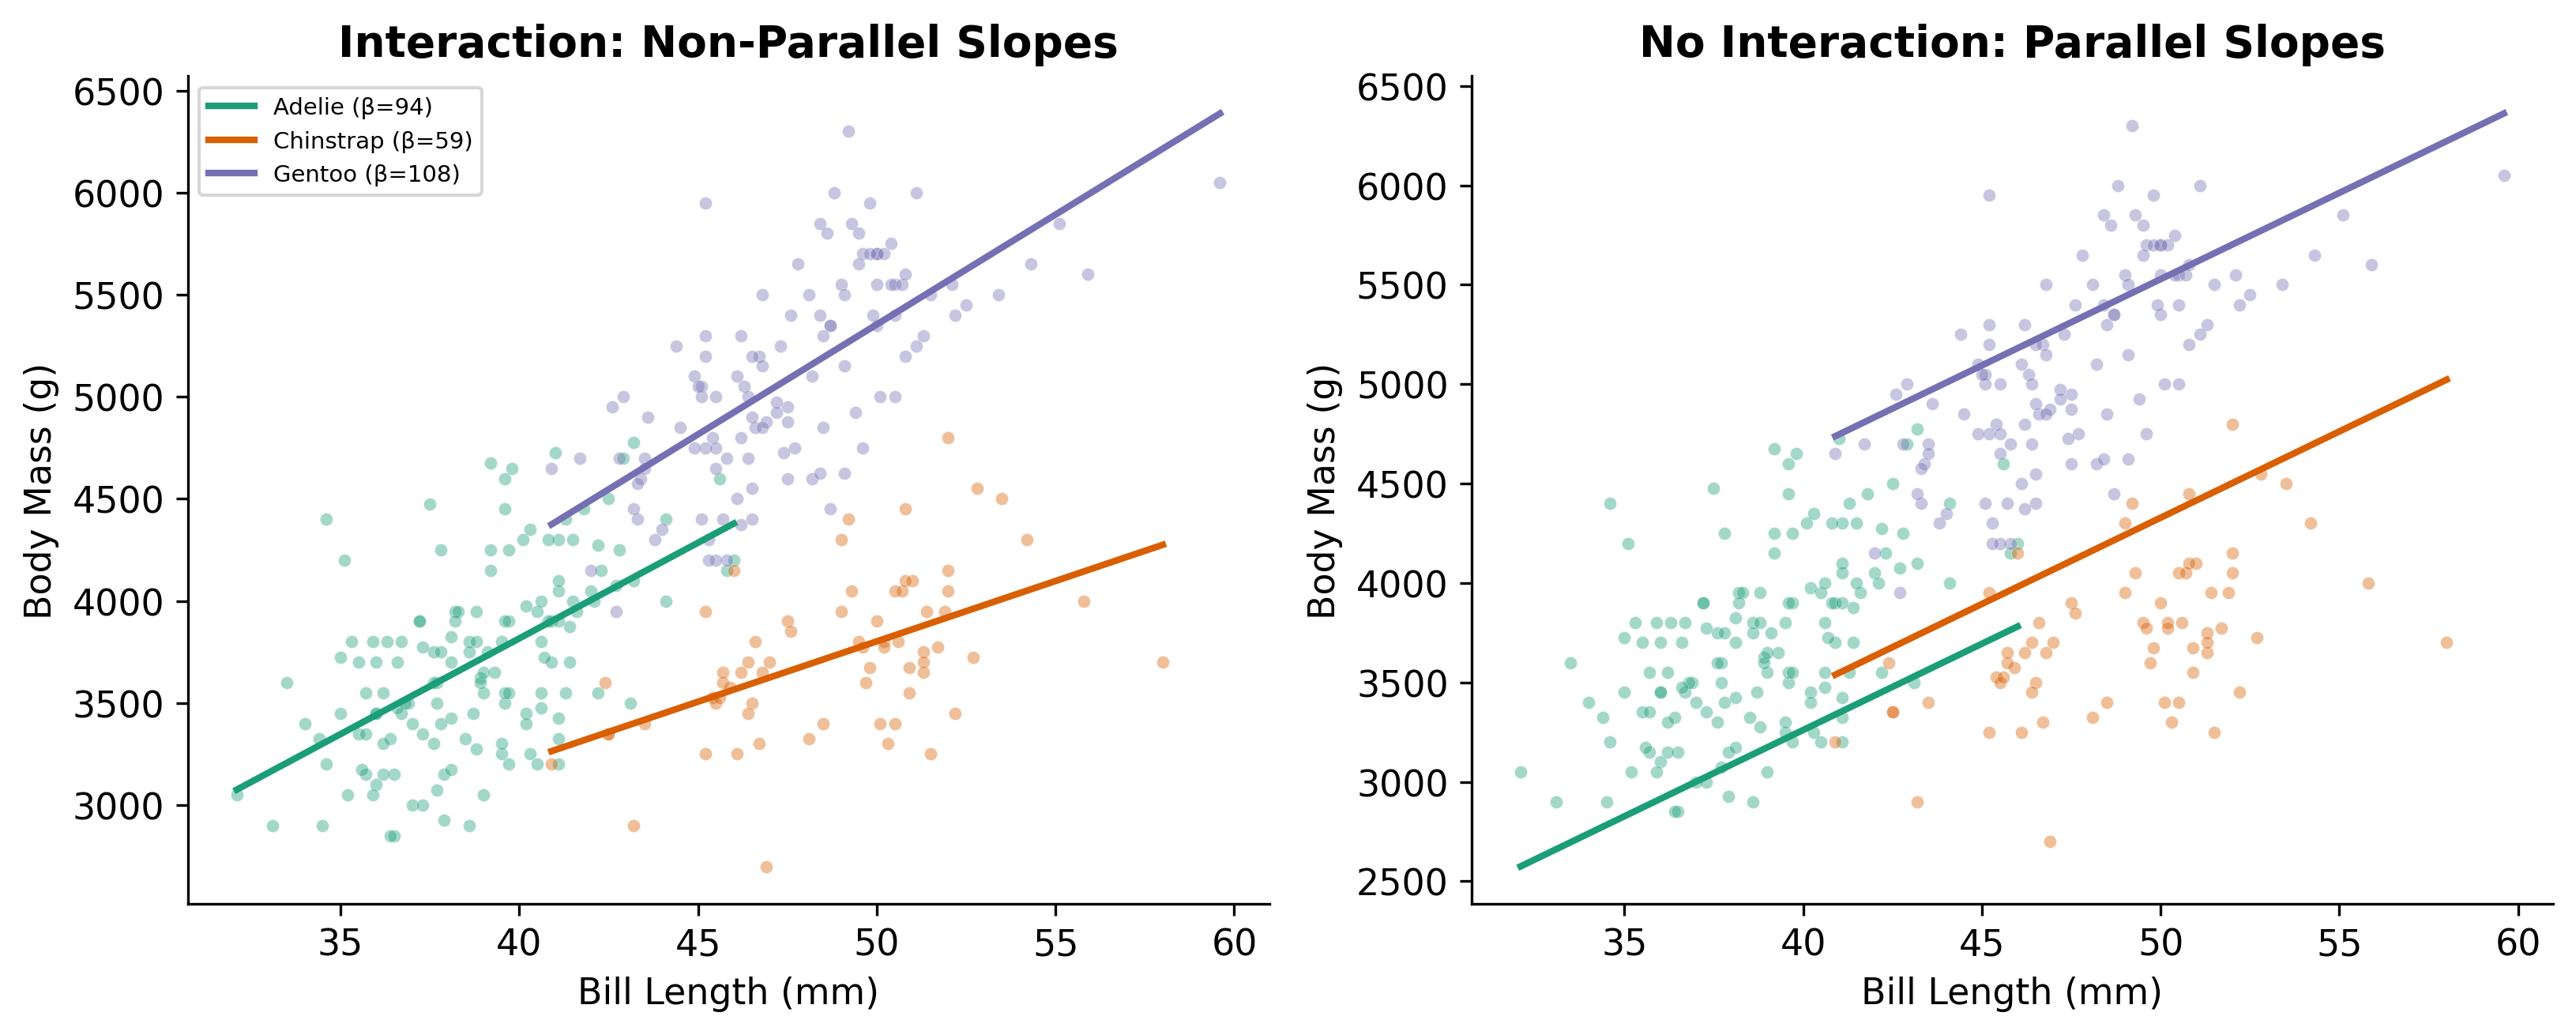
\includegraphics[width=0.88\textwidth]{m2_5_interaction_slopes.png}

\vspace{0.2cm}
\begin{columns}[T]
\begin{column}{0.48\textwidth}
\begin{exampleblock}{Data Insight}
    \scriptsize Left: slopes differ by species --- the effect of bill length on mass \textbf{depends on species}. This is an interaction. Right: parallel slopes --- the effect is the same regardless of species (no interaction).
\end{exampleblock}
\end{column}
\begin{column}{0.48\textwidth}
\begin{alertblock}{Pro-Tip}
    \scriptsize Visual test: if the lines are not parallel, there is likely an interaction. Formal test: include \texttt{bill\_length:species} (R) or \texttt{bill\_length*species} and check its $p$-value.
\end{alertblock}
\end{column}
\end{columns}
\end{frame}

% ── 124 ──
\begin{frame}{Interaction in the Model Formula}
\smark{124/300}
\centering\small
\begin{tabular}{@{}lll@{}}
    \toprule
    \textbf{R Formula} & \textbf{Python (statsmodels)} & \textbf{Meaning} \\
    \midrule
    \texttt{y \textasciitilde\ x + g}   & \texttt{"y \textasciitilde\ x + g"}   & Main effects only (parallel) \\
    \texttt{y \textasciitilde\ x * g}   & \texttt{"y \textasciitilde\ x * g"}   & Main effects + interaction \\
    \texttt{y \textasciitilde\ x : g}   & \texttt{"y \textasciitilde\ x : g"}   & Interaction only (rare) \\
    \texttt{y \textasciitilde\ x * g * z}& \texttt{"y \textasciitilde\ x * g * z"}& All 2-way + 3-way \\
    \bottomrule
\end{tabular}

\vspace{0.3cm}
\begin{exampleblock}{Data Insight}
    \scriptsize \texttt{x * g} expands to \texttt{x + g + x:g}. The interaction term \texttt{x:g} allows the slope of \texttt{x} to differ by level of \texttt{g}. If $p_{\text{interaction}} < 0.05$, the slopes are statistically non-parallel.
\end{exampleblock}
\end{frame}

% ── 125 ──
\begin{frame}[fragile]{Fitting Interactions --- Code}\smark{125/300}
\begin{columns}[T]
\begin{column}{0.48\textwidth}
\begin{lstlisting}[style=Rstyle]
# Main effects only
m1 <- lm(body_mass_g ~
  bill_length_mm + species,
  data = penguins)

# With interaction
m2 <- lm(body_mass_g ~
  bill_length_mm * species,
  data = penguins)

# Compare
anova(m1, m2)
# If p < 0.05: interaction matters
\end{lstlisting}
\end{column}
\begin{column}{0.48\textwidth}
\begin{lstlisting}[style=Pystyle]
import statsmodels.formula.api as smf

# Main effects only
m1 = smf.ols(
    "body_mass_g ~ bill_length_mm "
    "+ species", data=penguins).fit()

# With interaction
m2 = smf.ols(
    "body_mass_g ~ bill_length_mm "
    "* species", data=penguins).fit()

# Compare
from statsmodels.stats.anova \
    import anova_lm
anova_lm(m1, m2)
\end{lstlisting}
\end{column}
\end{columns}
\end{frame}

% ── 126 ──
\begin{frame}{Simpson's Paradox}
\smark{126/300}
\centering
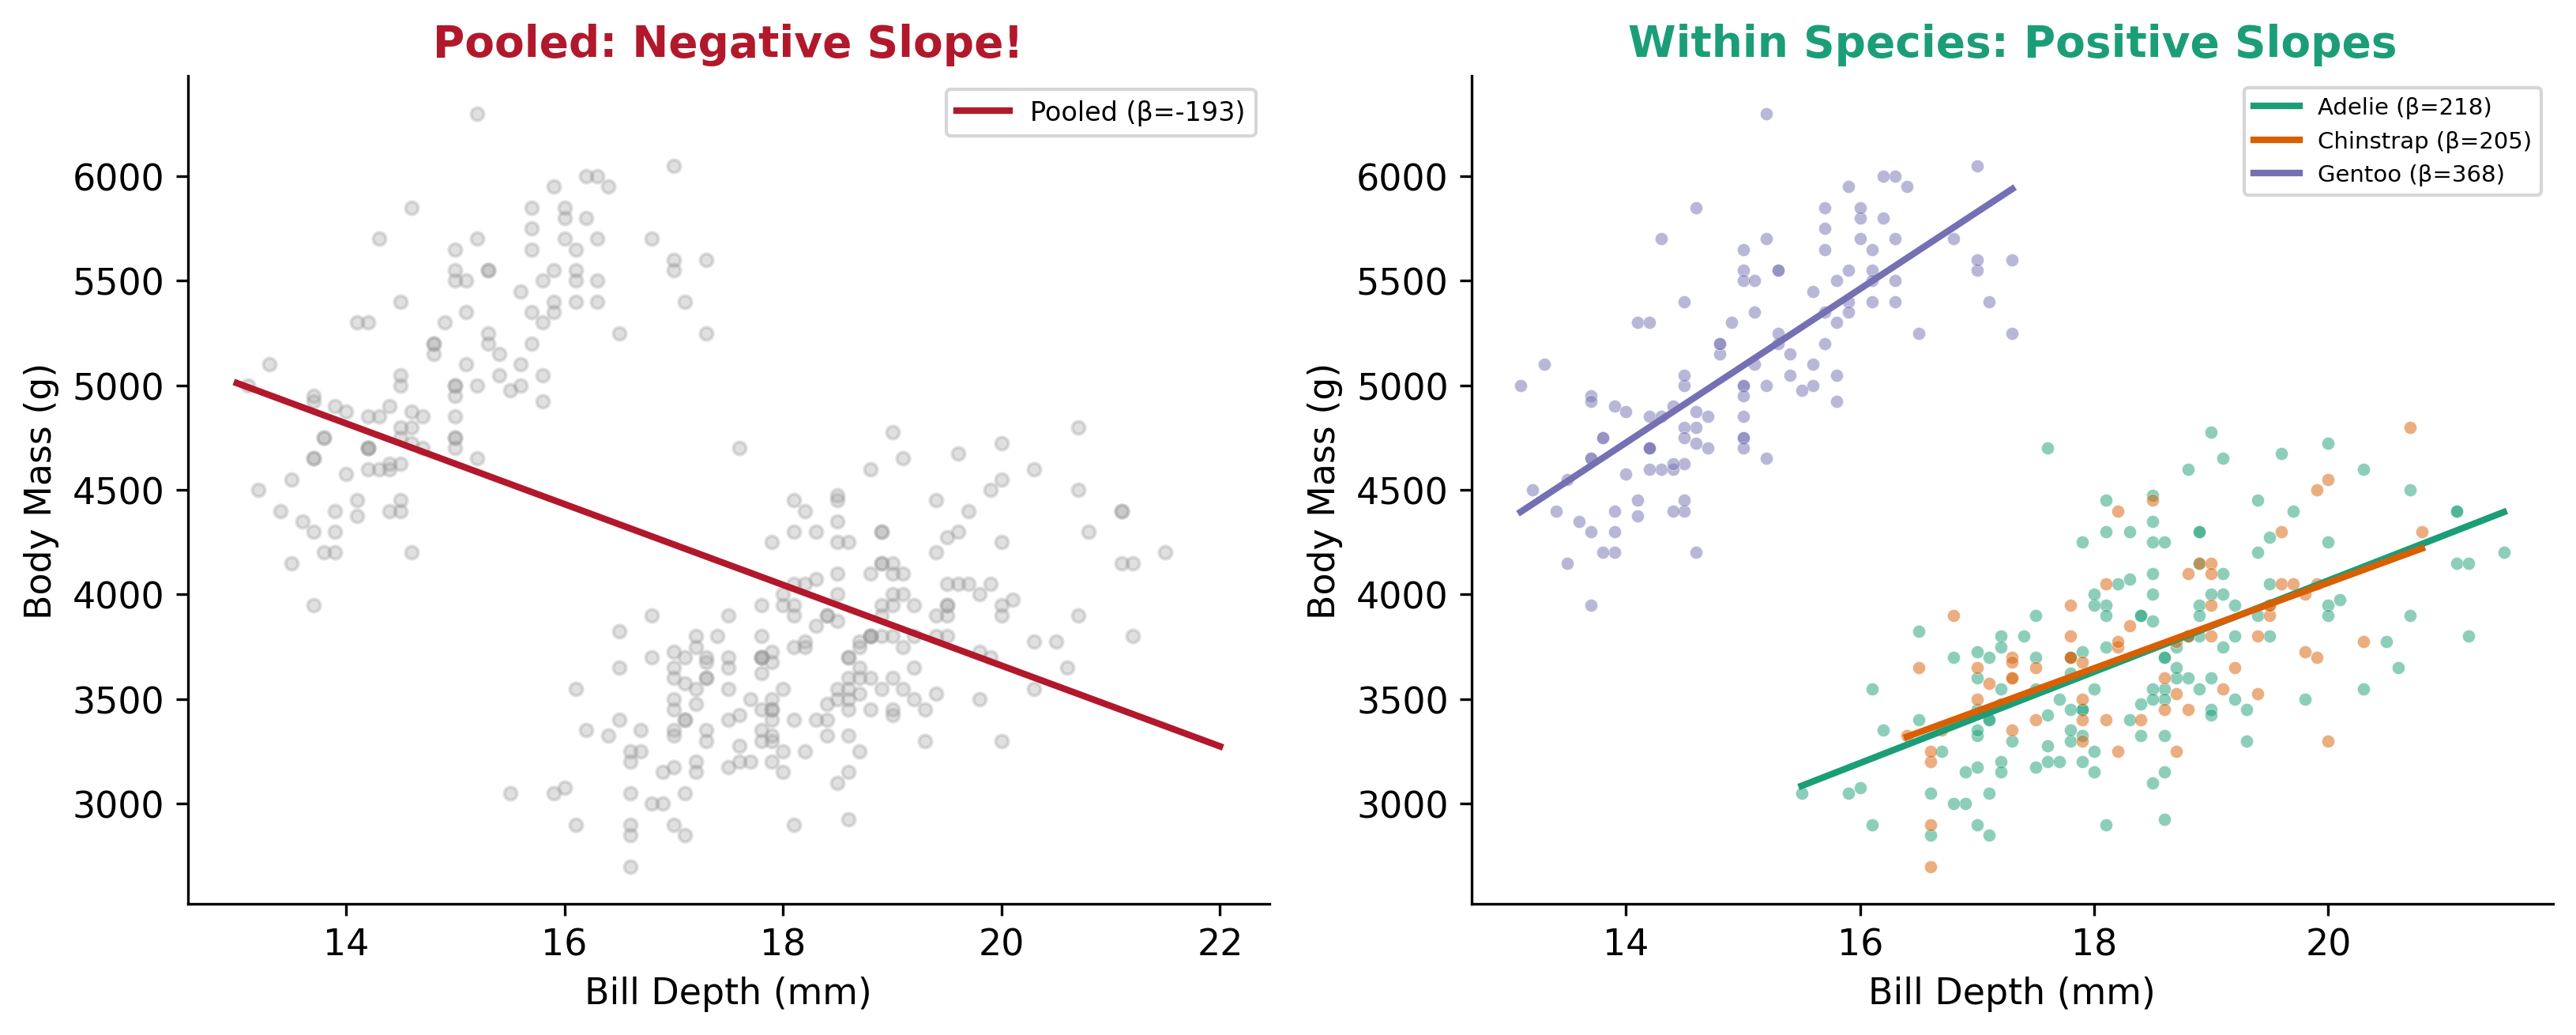
\includegraphics[width=0.88\textwidth]{m2_5_simpsons_paradox.png}

\vspace{0.2cm}
\begin{exampleblock}{Data Insight}
    \scriptsize Left: pooling all species, bill depth has a \textbf{negative} relationship with body mass ($\beta = -193$). Right: within each species, the relationship is \textbf{positive} ($\beta = +205$ to $+368$). The confound is species composition --- Gentoo have shallow bills but heavy bodies.
\end{exampleblock}
\end{frame}

% ── 127 ──
\begin{frame}{Detecting Simpson's Paradox Visually}
\smark{127/300}
\begin{columns}[T]
\begin{column}{0.50\textwidth}
\begin{itemize}
    \item Plot the scatter \textbf{without} group color $\to$ observe the pooled trend
    \item Add \texttt{color = group} $\to$ observe within-group trends
    \item If the slopes \textbf{reverse direction}, you have Simpson's paradox
    \item The fix: always include the confounding variable in the model
\end{itemize}
\end{column}
\begin{column}{0.47\textwidth}
\begin{alertblock}{Pro-Tip}
    \scriptsize Simpson's paradox is not a rare curiosity --- it appears in medical trials, educational data, university admissions (Berkeley), and ecological studies. Always check group-level trends before reporting pooled effects.
\end{alertblock}
\end{column}
\end{columns}
\end{frame}

% ── 128 ──
\begin{frame}{Interaction Plots: Categorical $\times$ Categorical}
\smark{128/300}
\centering
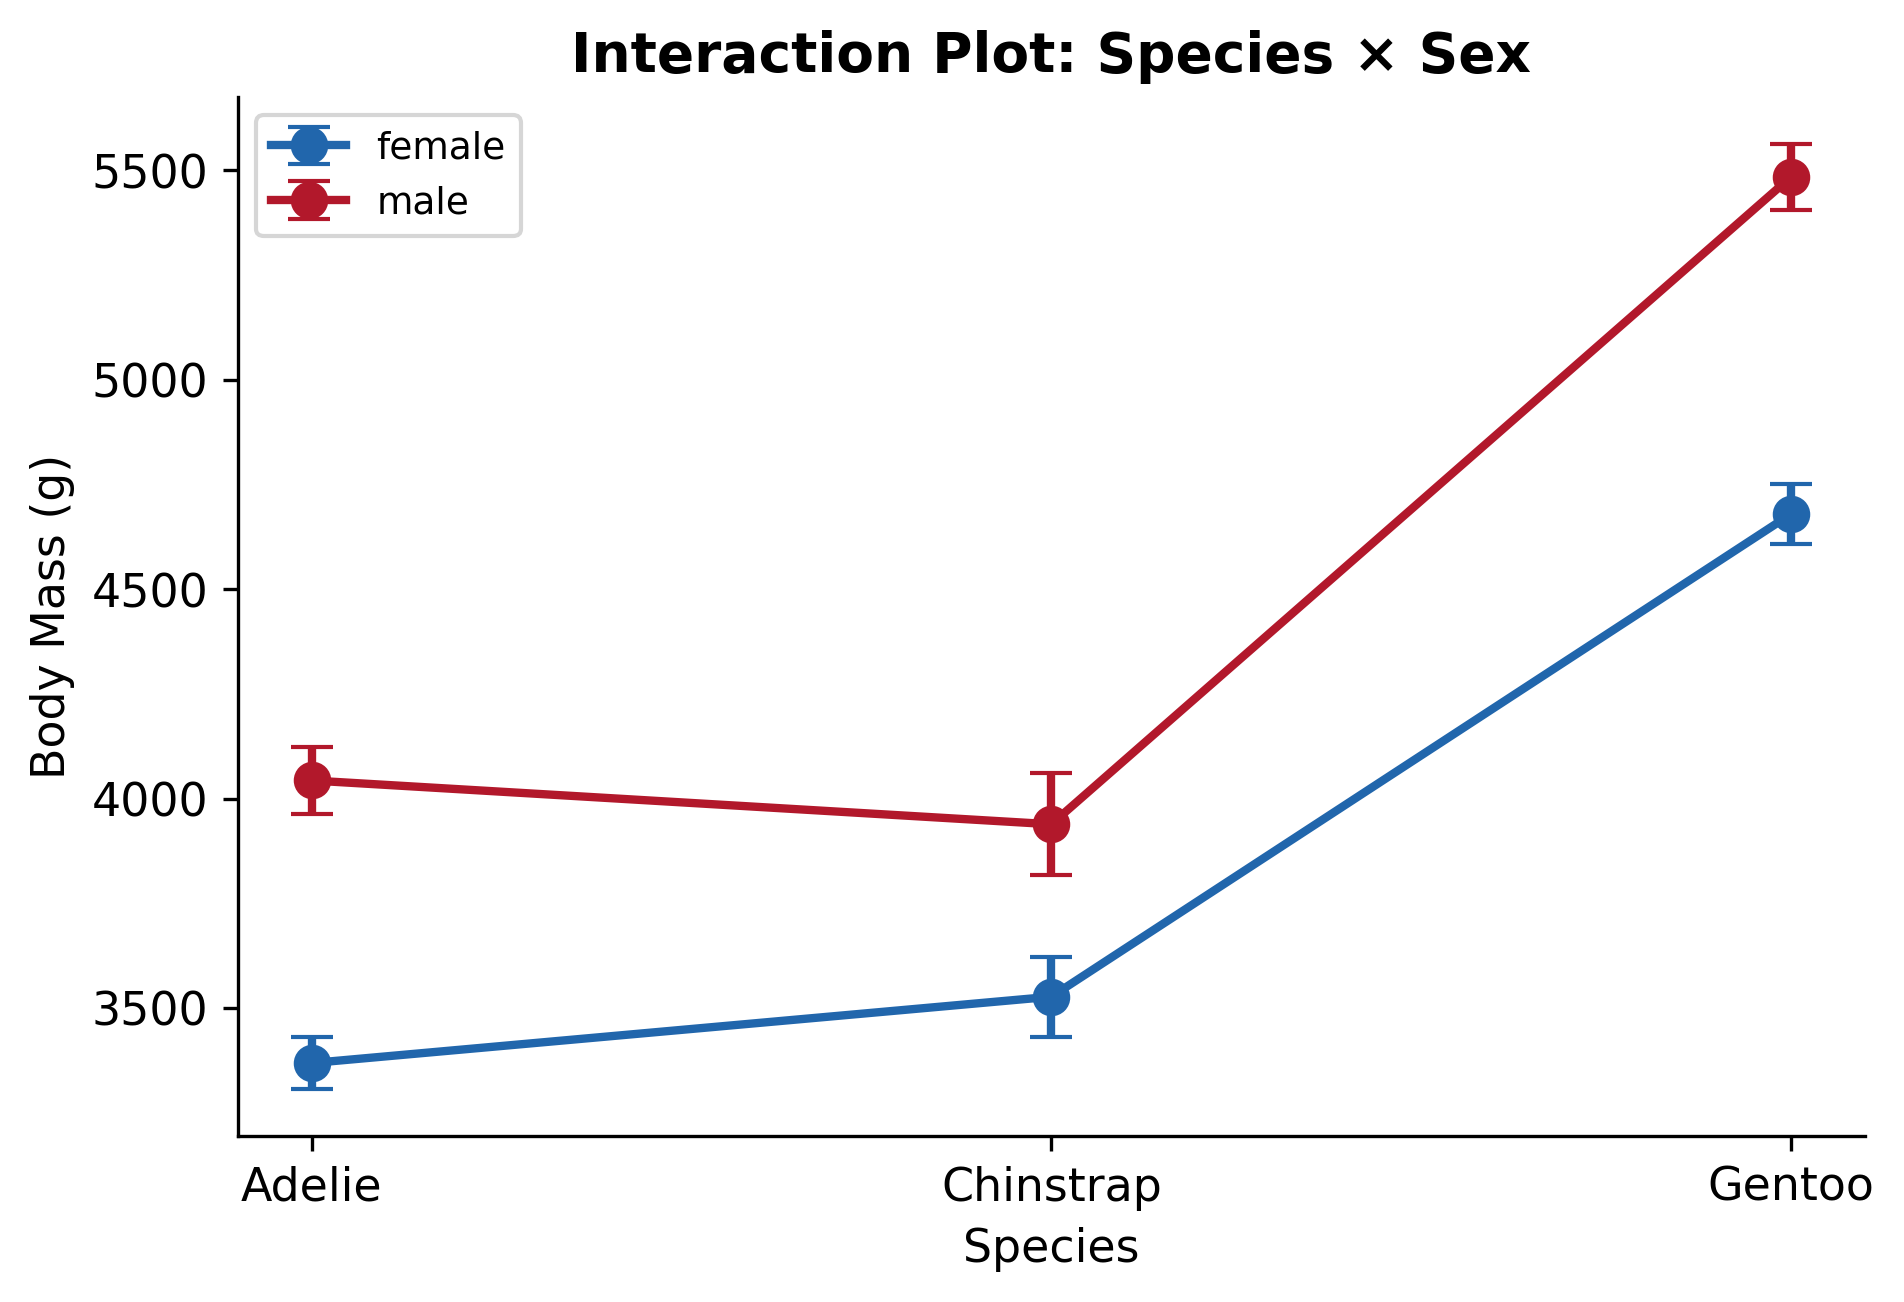
\includegraphics[width=0.68\textwidth]{m2_5_interaction_plot.png}

\vspace{0.2cm}
\begin{columns}[T]
\begin{column}{0.48\textwidth}
\begin{itemize}
    \item $x$-axis = factor A (species)
    \item Lines/colors = factor B (sex)
    \item $y$-axis = group mean $\pm$ CI
    \item \textbf{Parallel lines} = no interaction
    \item \textbf{Crossing or diverging lines} = interaction
\end{itemize}
\end{column}
\begin{column}{0.48\textwidth}
\begin{exampleblock}{Data Insight}
    \scriptsize The sex gap is roughly constant across species ($\sim$700\,g) --- lines are nearly parallel. A significant interaction would show the gap widening or narrowing across species.
\end{exampleblock}
\end{column}
\end{columns}
\end{frame}

% ── 129 ──
\begin{frame}[fragile]{Interaction Plot --- \Rlang}\smark{129/300}
\begin{columns}[T]
\begin{column}{0.55\textwidth}
\begin{lstlisting}[style=Rstyle]
# Base approach: stat_summary
ggplot(penguins,
  aes(species, body_mass_g,
      color = sex, group = sex)) +
  stat_summary(fun.data=mean_se,
    geom="pointrange") +
  stat_summary(fun=mean,
    geom="line") +
  scale_color_manual(
    values=c("#2166AC","#B2182B"))+
  theme_minimal()

# emmeans approach (cleaner)
library(emmeans)
emmip(model, sex ~ species,
  CIs = TRUE)
\end{lstlisting}
\end{column}
\begin{column}{0.42\textwidth}
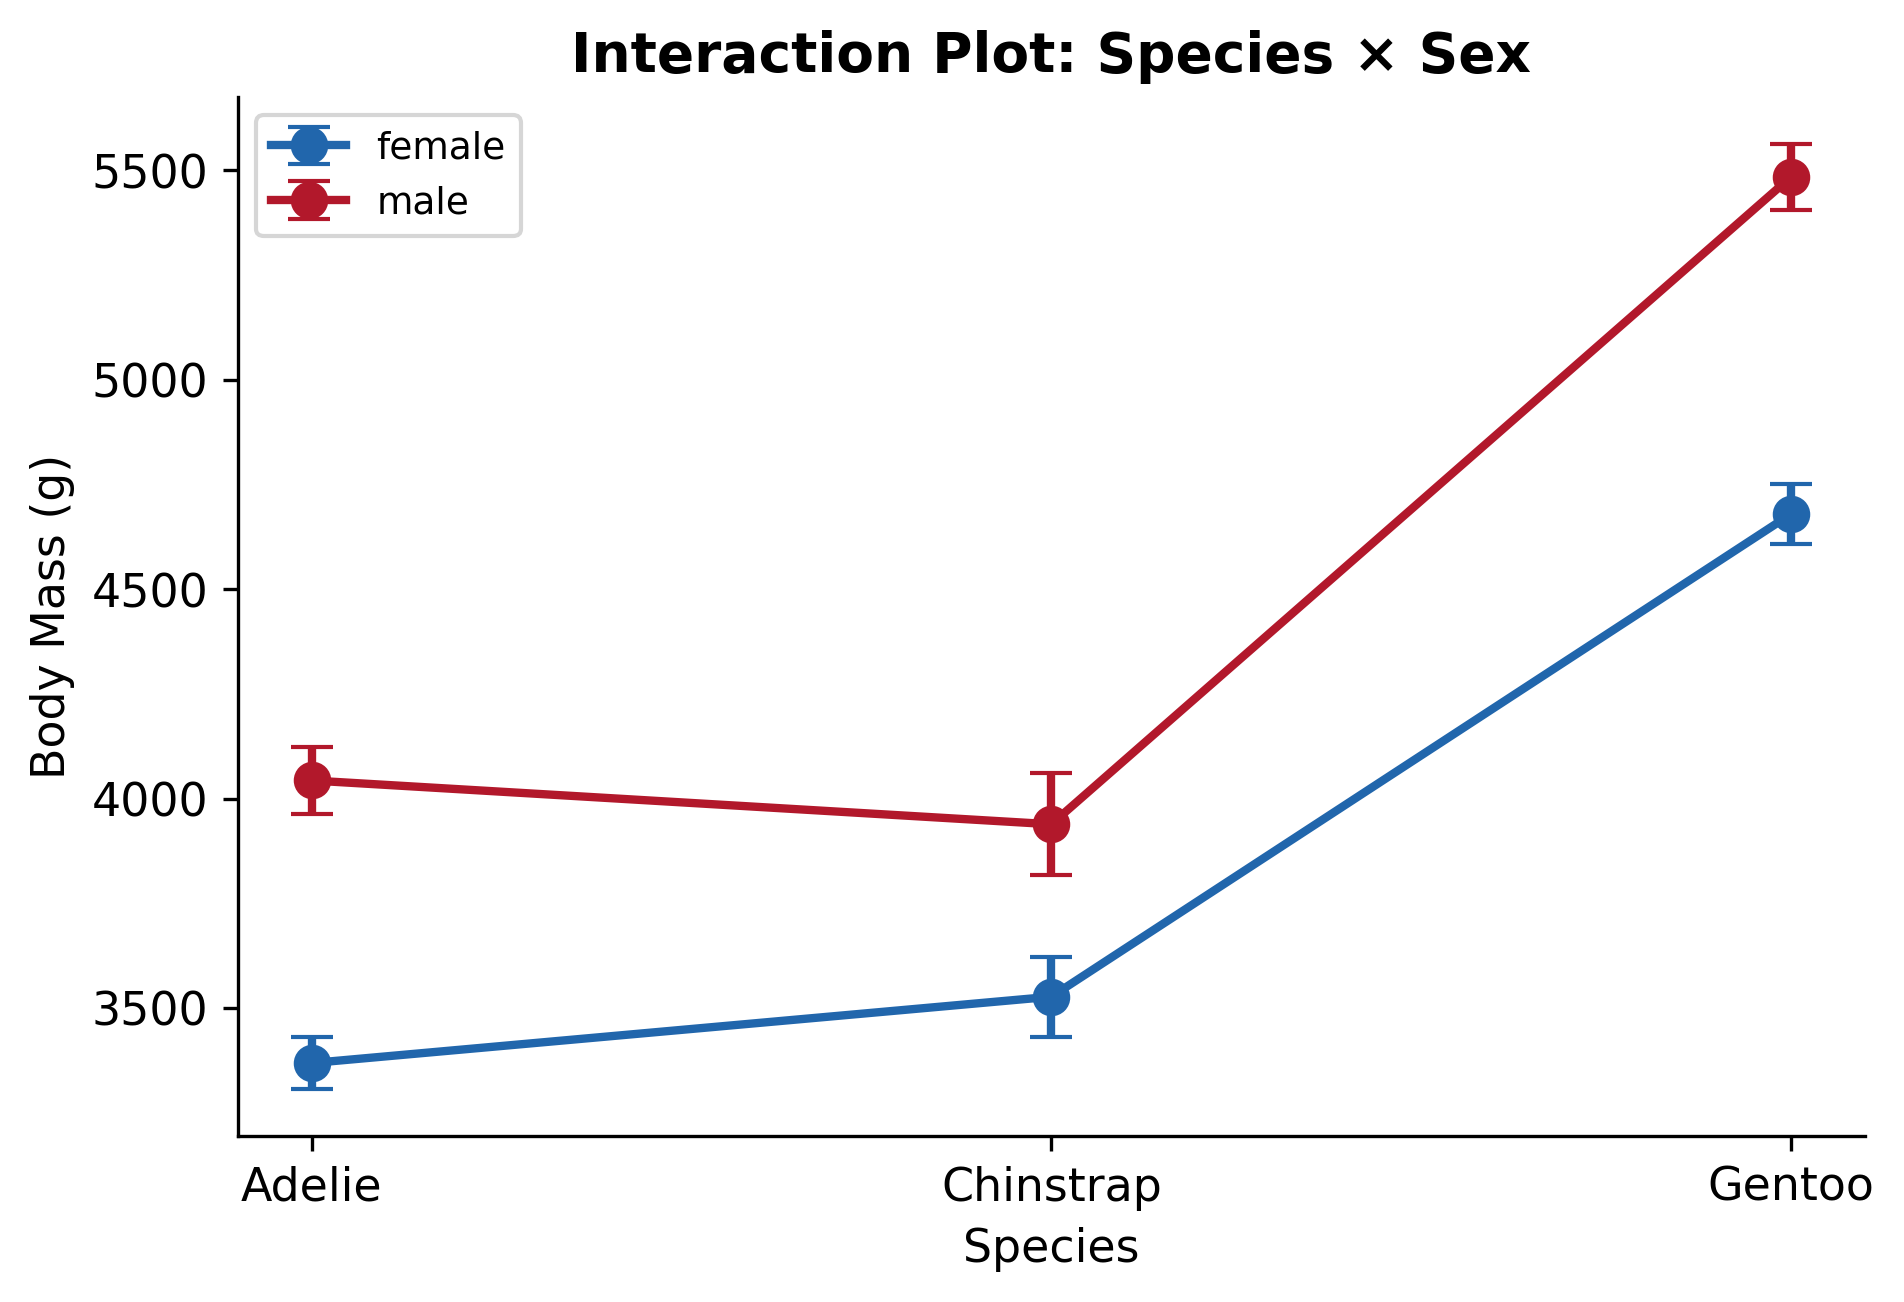
\includegraphics[width=\textwidth]{m2_5_interaction_plot.png}
\begin{alertblock}{Pro-Tip}
    \scriptsize \texttt{emmeans::emmip()} generates interaction plots from the \emph{model}, not the raw data. This ensures the plot reflects the model's estimated means, not raw sample means.
\end{alertblock}
\end{column}
\end{columns}
\end{frame}

% ── 130 ──
\begin{frame}[fragile]{Interaction Plot --- \Python}\smark{130/300}
\begin{columns}[T]
\begin{column}{0.55\textwidth}
\begin{lstlisting}[style=Pystyle]
# seaborn pointplot
sns.pointplot(data=penguins,
    x="species", y="body_mass_g",
    hue="sex", errorbar="se",
    capsize=0.1, dodge=0.1,
    palette=["#2166AC","#B2182B"],
    markers=["o","s"],
    linestyles=["-","--"])

# Manual from model predictions
pred = model.get_prediction(X_grid)
ci = pred.summary_frame(alpha=0.05)
# Plot mean + CI per cell
\end{lstlisting}
\end{column}
\begin{column}{0.42\textwidth}
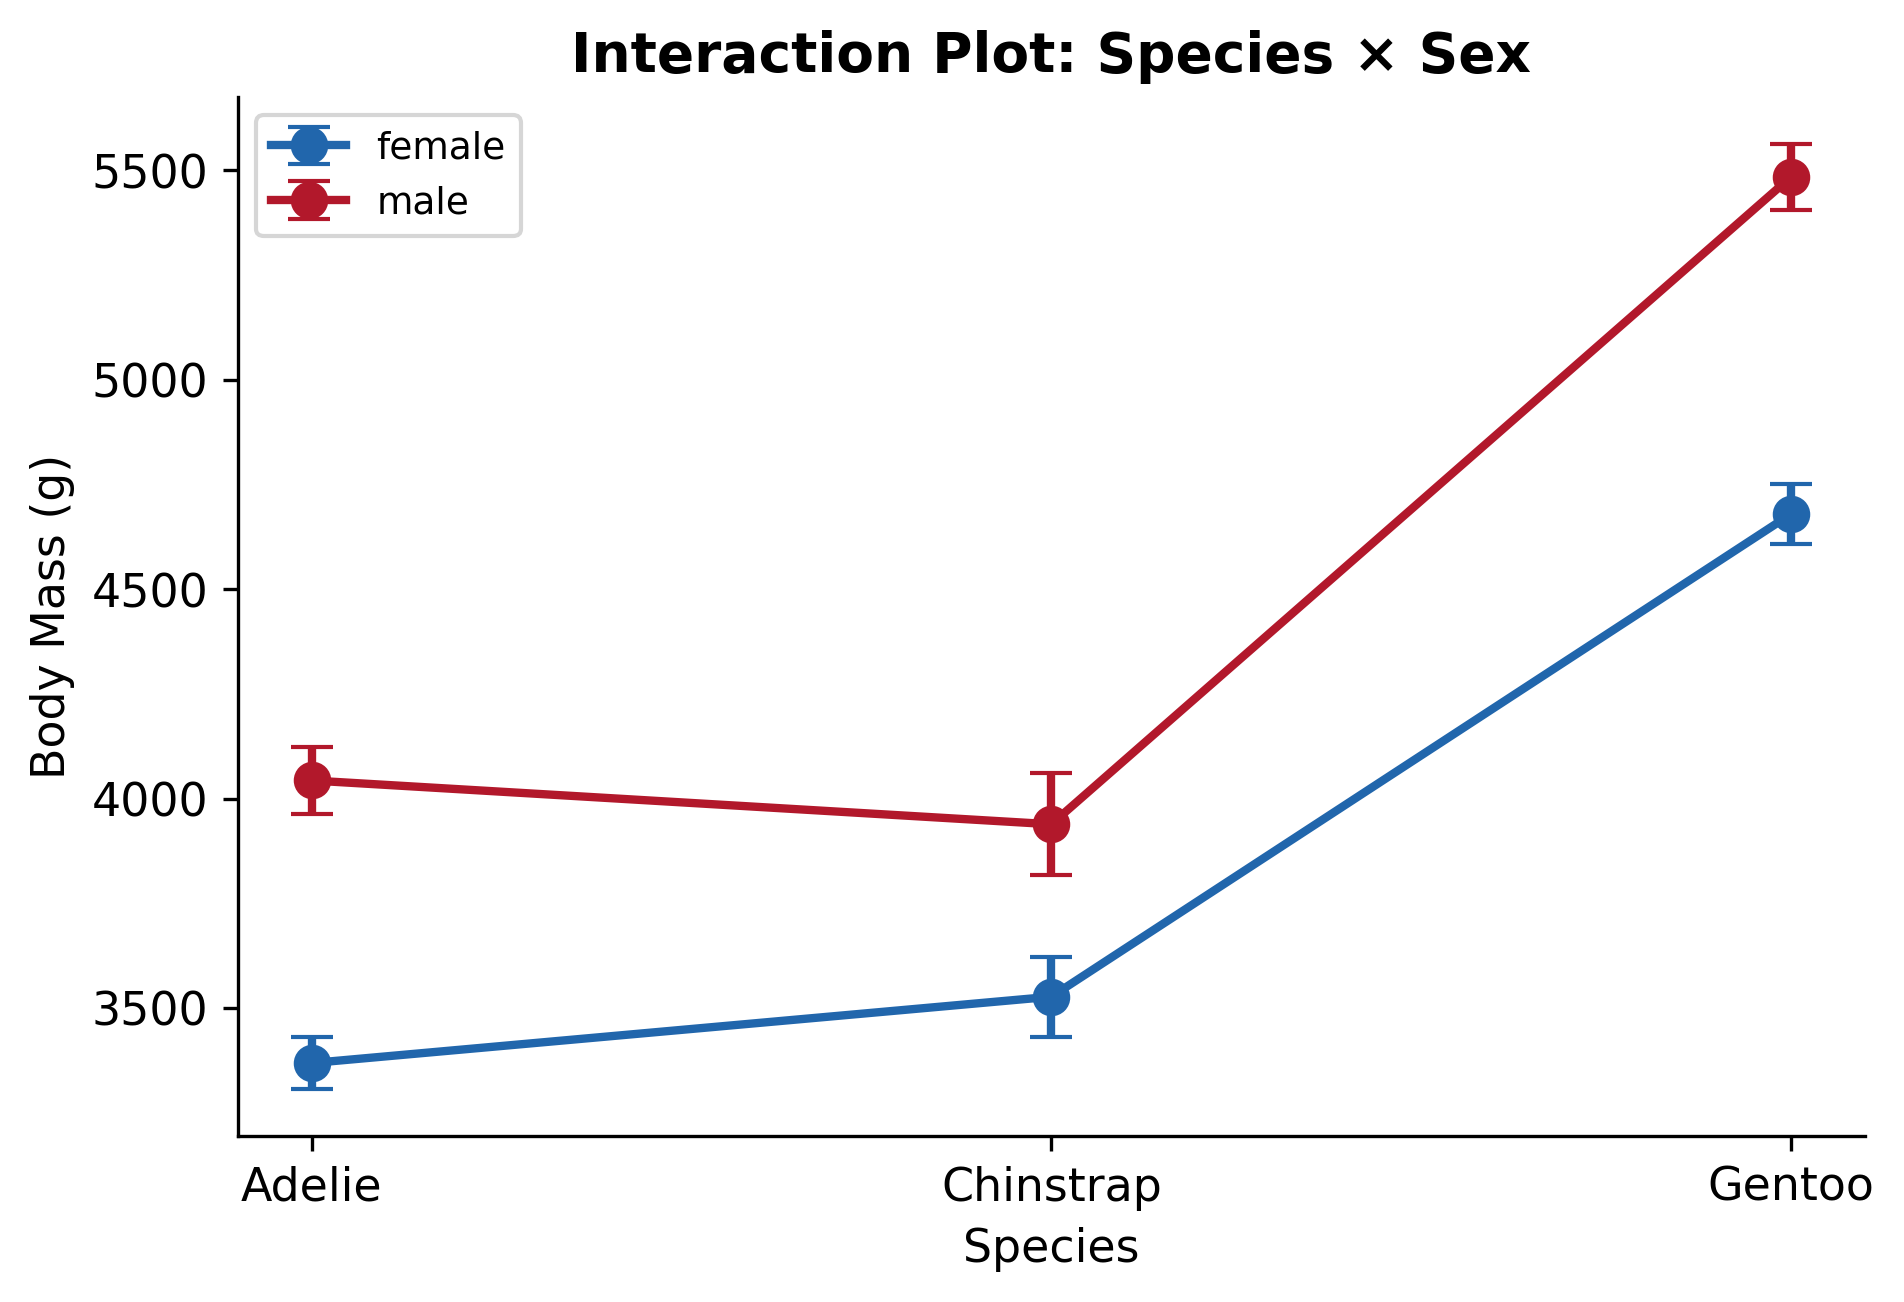
\includegraphics[width=\textwidth]{m2_5_interaction_plot.png}
\begin{exampleblock}{Data Insight}
    \scriptsize \texttt{sns.pointplot()} with \texttt{hue=} produces an interaction plot automatically. Add \texttt{dodge=0.1} to offset overlapping error bars.
\end{exampleblock}
\end{column}
\end{columns}
\end{frame}

% ── 131 ──
\begin{frame}{Marginal Effects: Continuous $\times$ Categorical}
\smark{131/300}
\centering
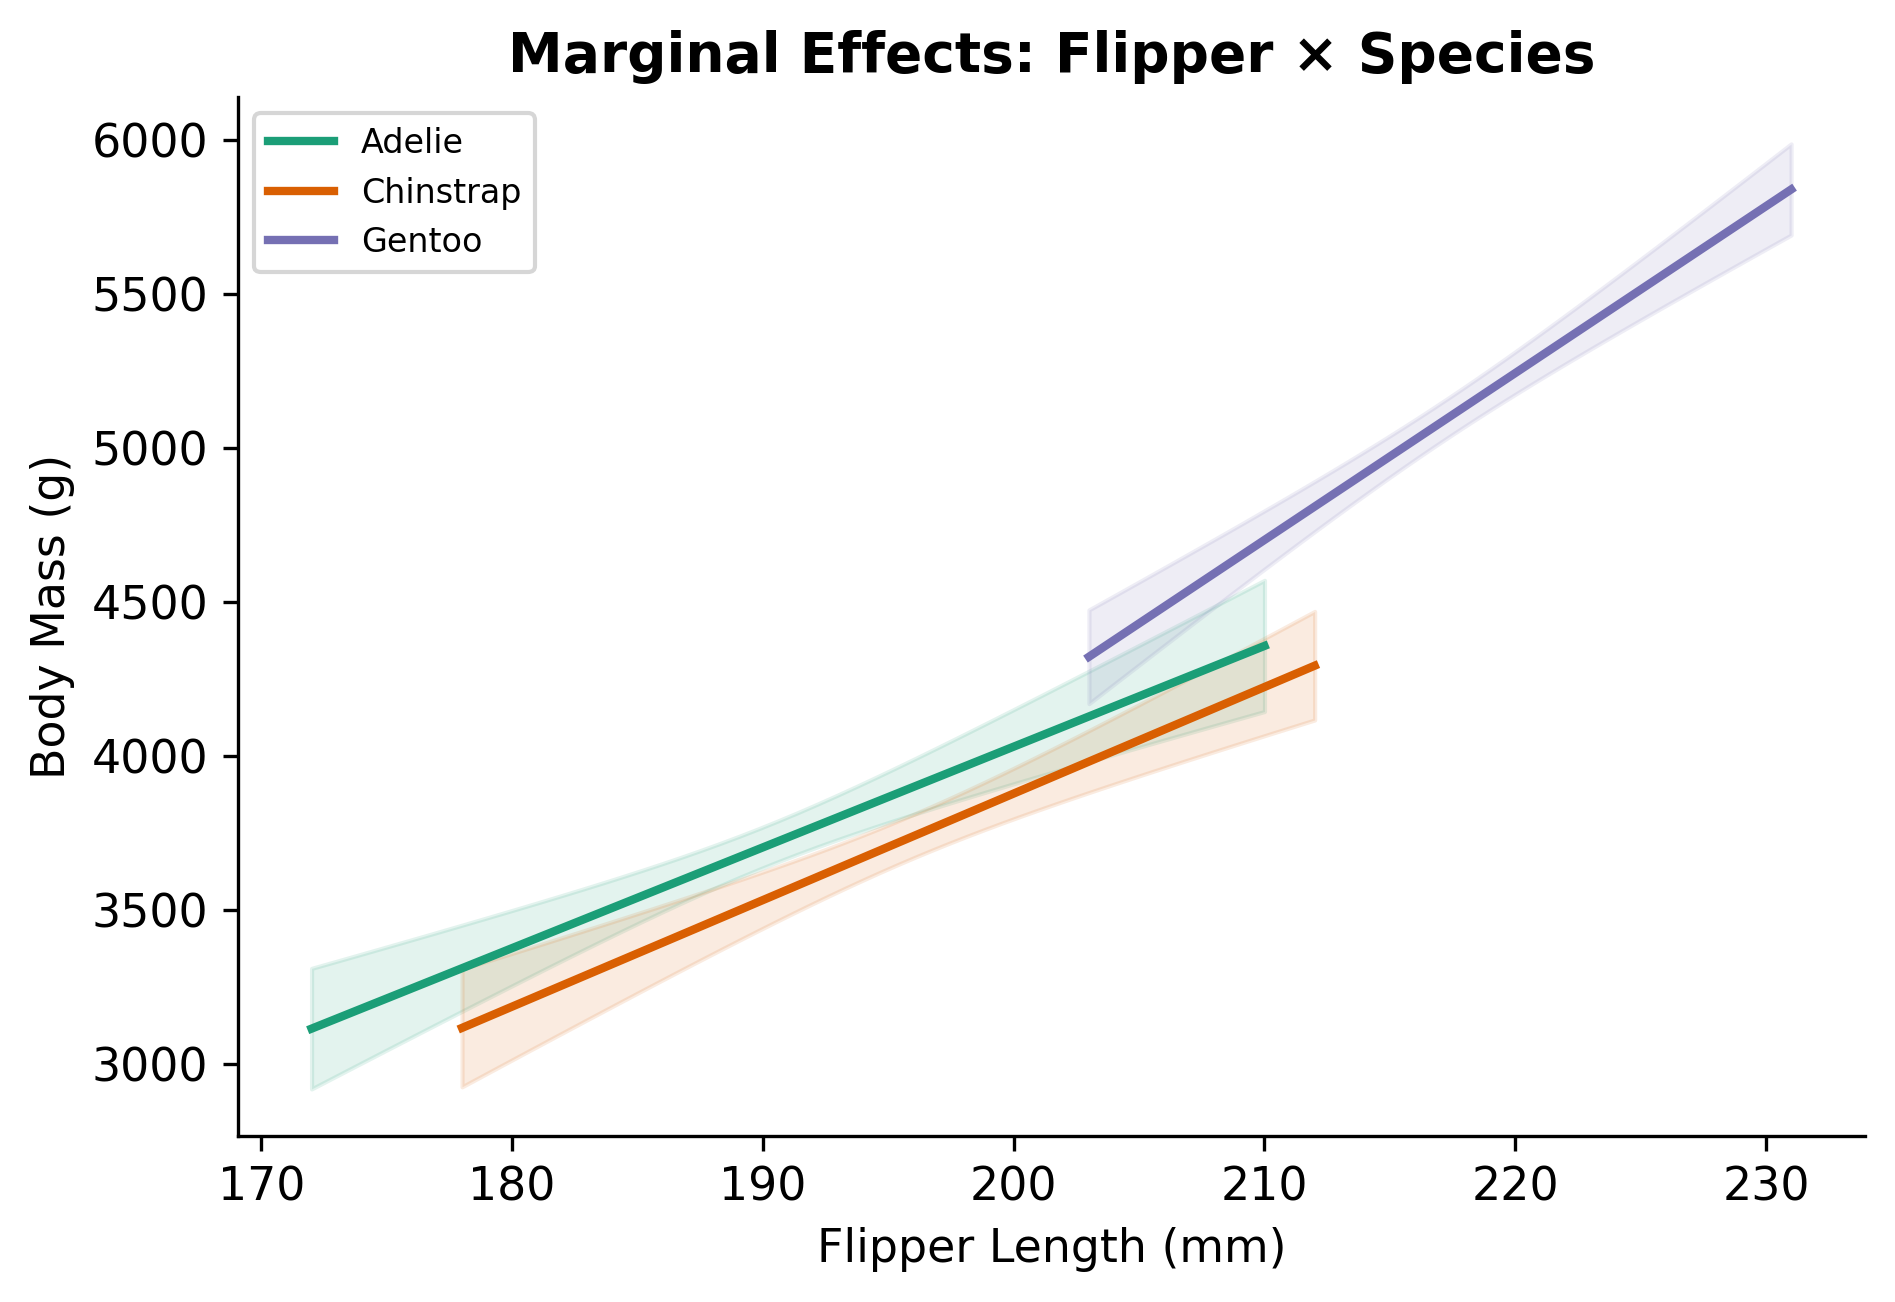
\includegraphics[width=0.68\textwidth]{m2_5_marginal_effects.png}

\vspace{0.2cm}
\begin{columns}[T]
\begin{column}{0.48\textwidth}
\begin{itemize}
    \item Regression line per group with CI bands
    \item Shows how the continuous predictor's effect varies by group
    \item The visual equivalent of reporting interaction coefficients
\end{itemize}
\end{column}
\begin{column}{0.48\textwidth}
\begin{exampleblock}{Data Insight}
    \scriptsize Gentoo (purple) have a steeper slope: each mm of flipper length adds more mass than for Adelie or Chinstrap. This is the interaction in action --- the \emph{rate} of change depends on species.
\end{exampleblock}
\end{column}
\end{columns}
\end{frame}

% ── 132 ──
\begin{frame}[fragile]{Marginal Effects --- Code}\smark{132/300}
\begin{columns}[T]
\begin{column}{0.48\textwidth}
\begin{lstlisting}[style=Rstyle]
# ggplot2: automatic via color
ggplot(penguins,
  aes(flipper_length_mm,
      body_mass_g,
      color = species)) +
  geom_point(alpha = 0.3) +
  geom_smooth(method = "lm") +
  theme_minimal()

# From model: marginaleffects
library(marginaleffects)
plot_predictions(model,
  condition = c("flipper_length_mm",
                "species"))
\end{lstlisting}
\end{column}
\begin{column}{0.48\textwidth}
\begin{lstlisting}[style=Pystyle]
# seaborn lmplot
sns.lmplot(data=penguins,
    x="flipper_length_mm",
    y="body_mass_g",
    hue="species", ci=95,
    palette=["#1B9E77","#D95F02",
             "#7570B3"],
    height=4, aspect=1.4)

# From model predictions
# Generate prediction grid:
grid = pd.DataFrame(...)
pred = model.get_prediction(
    sm.add_constant(grid))
\end{lstlisting}
\end{column}
\end{columns}
\end{frame}

% ── 133 ──
\begin{frame}{Estimated Marginal Means (emmeans)}
\smark{133/300}
\centering
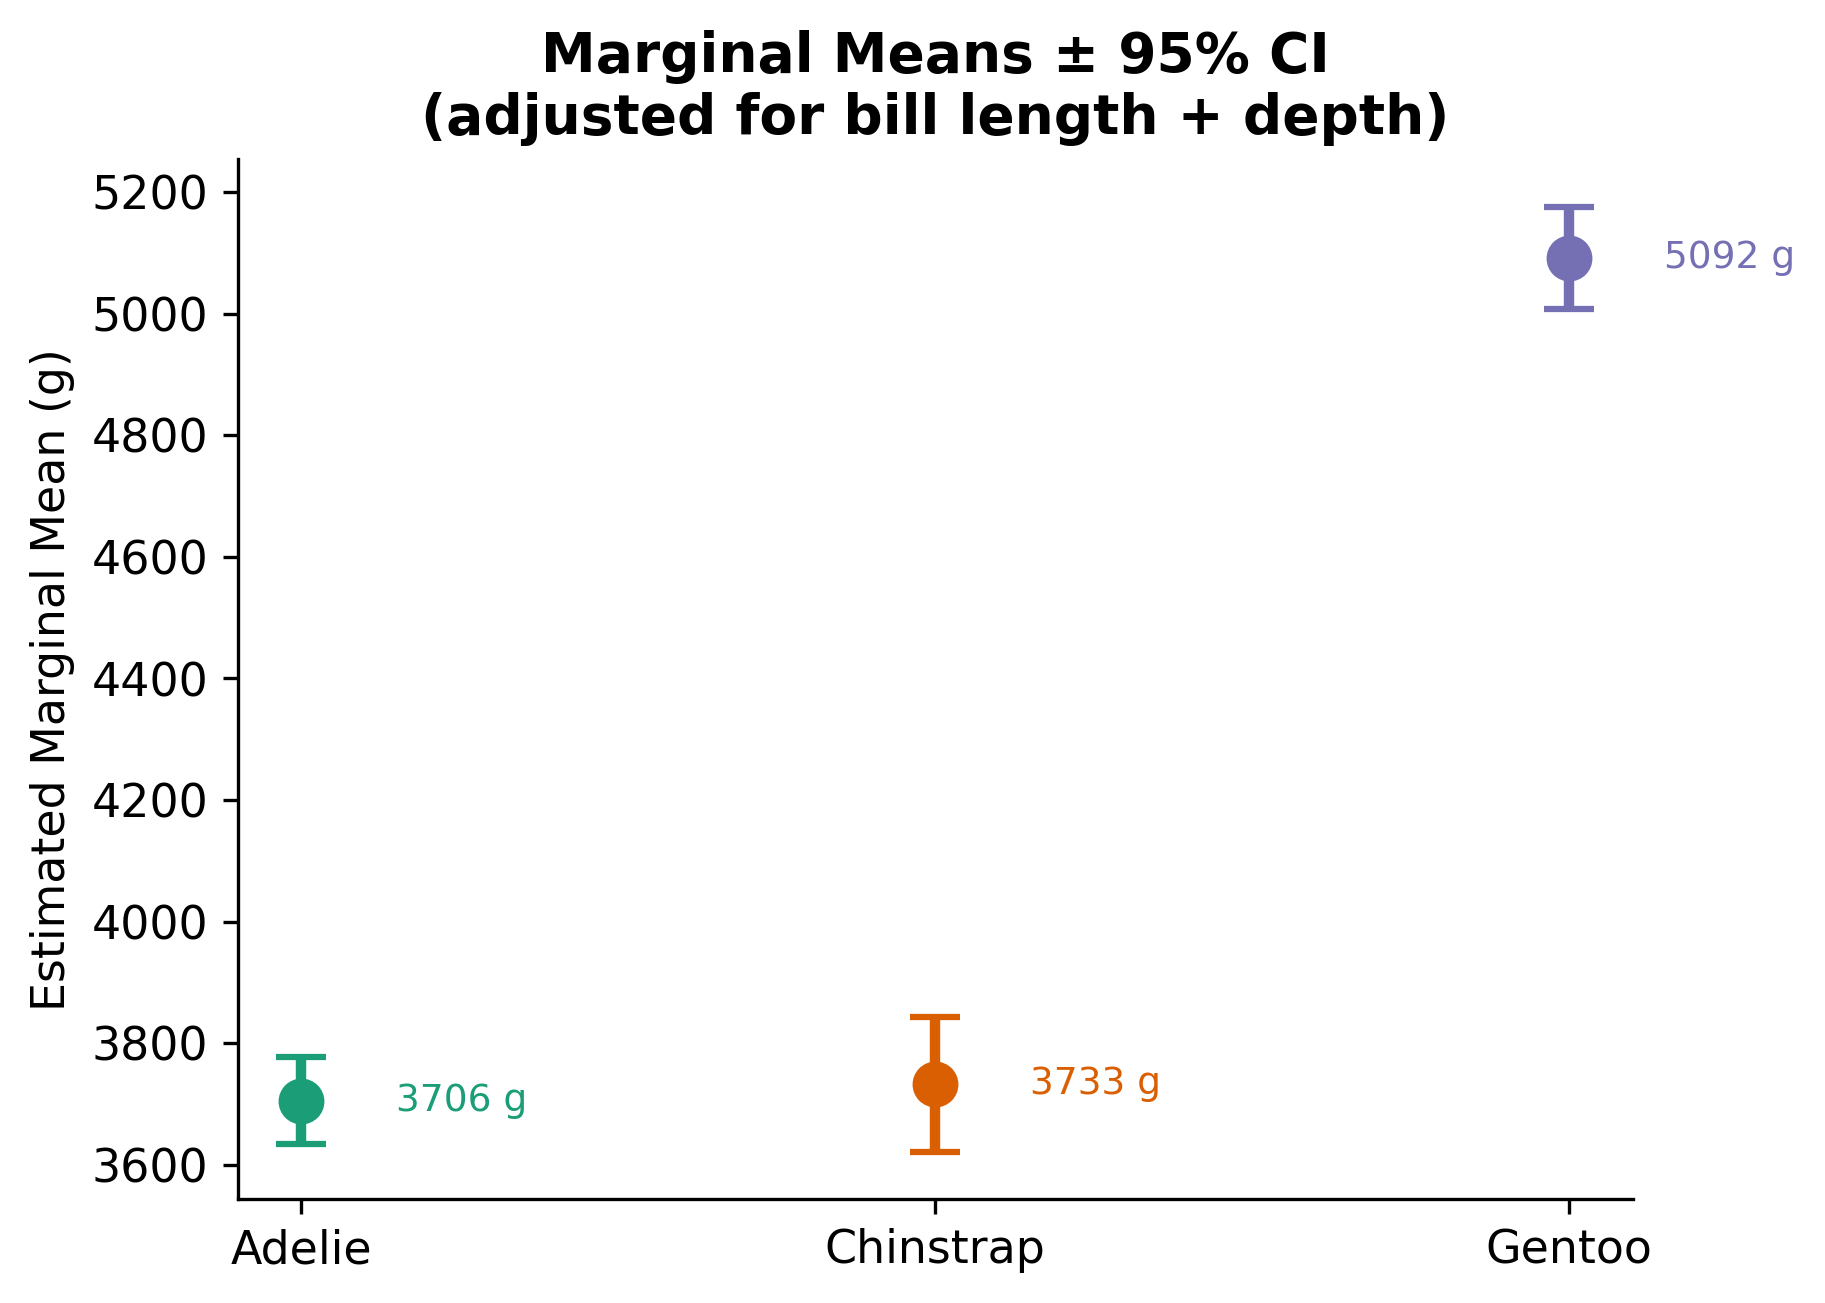
\includegraphics[width=0.62\textwidth]{m2_5_marginal_means.png}

\vspace{0.2cm}
\begin{columns}[T]
\begin{column}{0.48\textwidth}
\begin{itemize}
    \item Also called \textbf{least-squares means} or \textbf{adjusted means}
    \item Means from the \textbf{model}, not raw data
    \item Adjusted for covariates (held at their means)
    \item The correct way to compare groups when covariates are present
\end{itemize}
\end{column}
\begin{column}{0.48\textwidth}
\begin{alertblock}{Pro-Tip}
    \scriptsize Raw means can be misleading when groups differ on covariates. emmeans adjust for this: they answer ``what would the mean be if all groups had the same covariate values?''
\end{alertblock}
\end{column}
\end{columns}
\end{frame}

% ── 134 ──
\begin{frame}[fragile]{emmeans --- \Rlang}\smark{134/300}
\begin{columns}[T]
\begin{column}{0.55\textwidth}
\begin{lstlisting}[style=Rstyle]
library(emmeans)

model <- lm(body_mass_g ~
  bill_length_mm + bill_depth_mm +
  species, data = penguins)

# Marginal means per species
emm <- emmeans(model, ~ species)
summary(emm, infer = TRUE)

# Plot
plot(emm) + theme_minimal()
# Or ggplot2 from summary
emmeans_df <- as.data.frame(emm)
ggplot(emmeans_df,
  aes(emmean,
      fct_reorder(species,emmean)))+
  geom_pointrange(
    aes(xmin=lower.CL,
        xmax=upper.CL),
    color="#2166AC")
\end{lstlisting}
\end{column}
\begin{column}{0.42\textwidth}
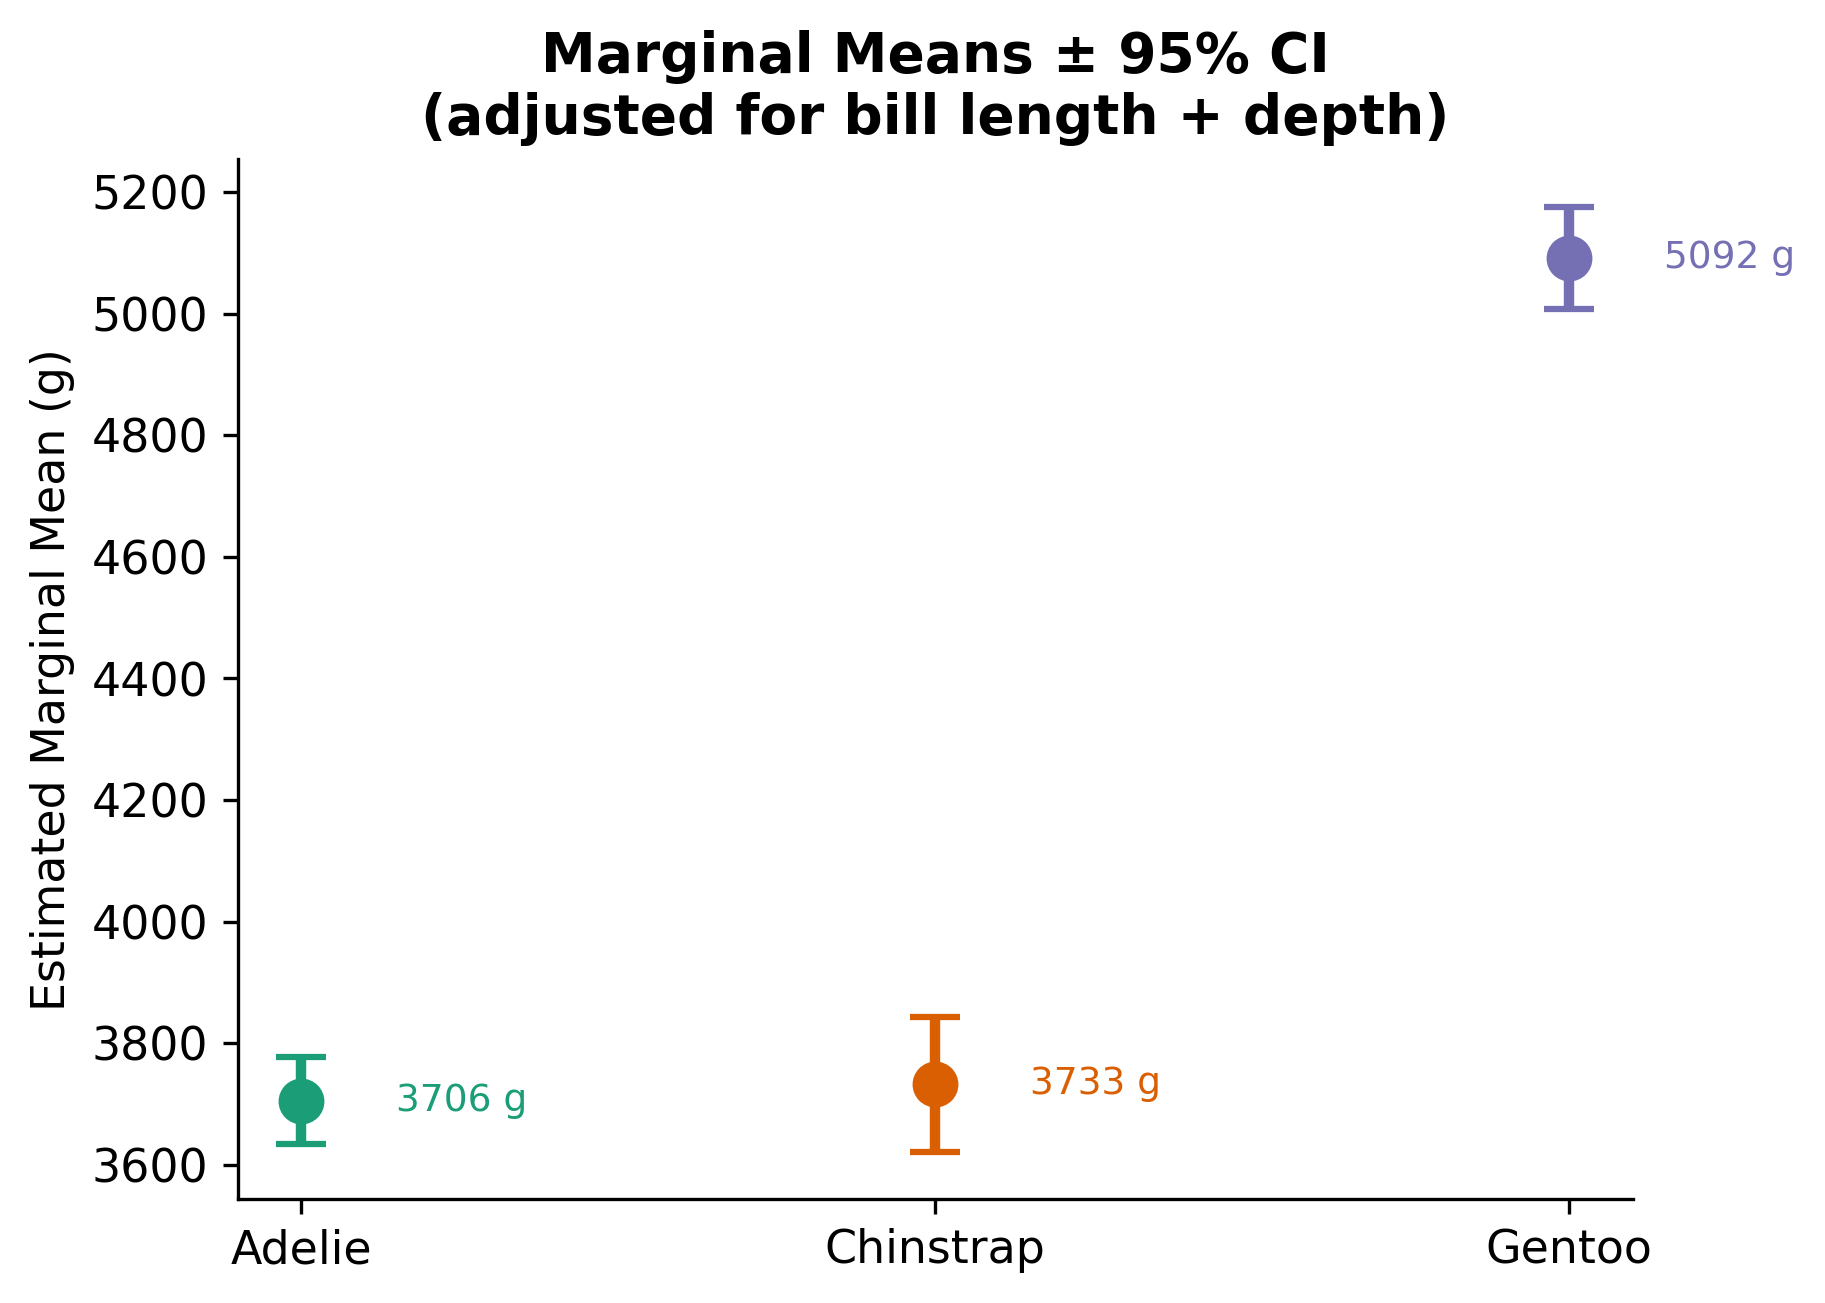
\includegraphics[width=\textwidth]{m2_5_marginal_means.png}
\begin{exampleblock}{Data Insight}
    \scriptsize \texttt{emmeans(model, \textasciitilde species)} computes the mean body mass for each species \emph{at the average bill length and depth}. This removes confounding by morphological differences.
\end{exampleblock}
\end{column}
\end{columns}
\end{frame}

% ── 135 ──
\begin{frame}[fragile]{emmeans --- \Python}\smark{135/300}
\begin{columns}[T]
\begin{column}{0.55\textwidth}
\begin{lstlisting}[style=Pystyle]
# No direct emmeans in Python.
# Approach 1: marginaleffects
# pip install marginaleffects
from marginaleffects import \
    predictions

pred = predictions(model,
    by="species")
# Returns adjusted means + CI

# Approach 2: manual
# Set covariates to their means
grid = pd.DataFrame({
    "species": species_list,
    "bill_length_mm": [bl_mean]*3,
    "bill_depth_mm": [bd_mean]*3})
X_grid = sm.add_constant(
    pd.get_dummies(grid))
pred = model.get_prediction(X_grid)
\end{lstlisting}
\end{column}
\begin{column}{0.42\textwidth}
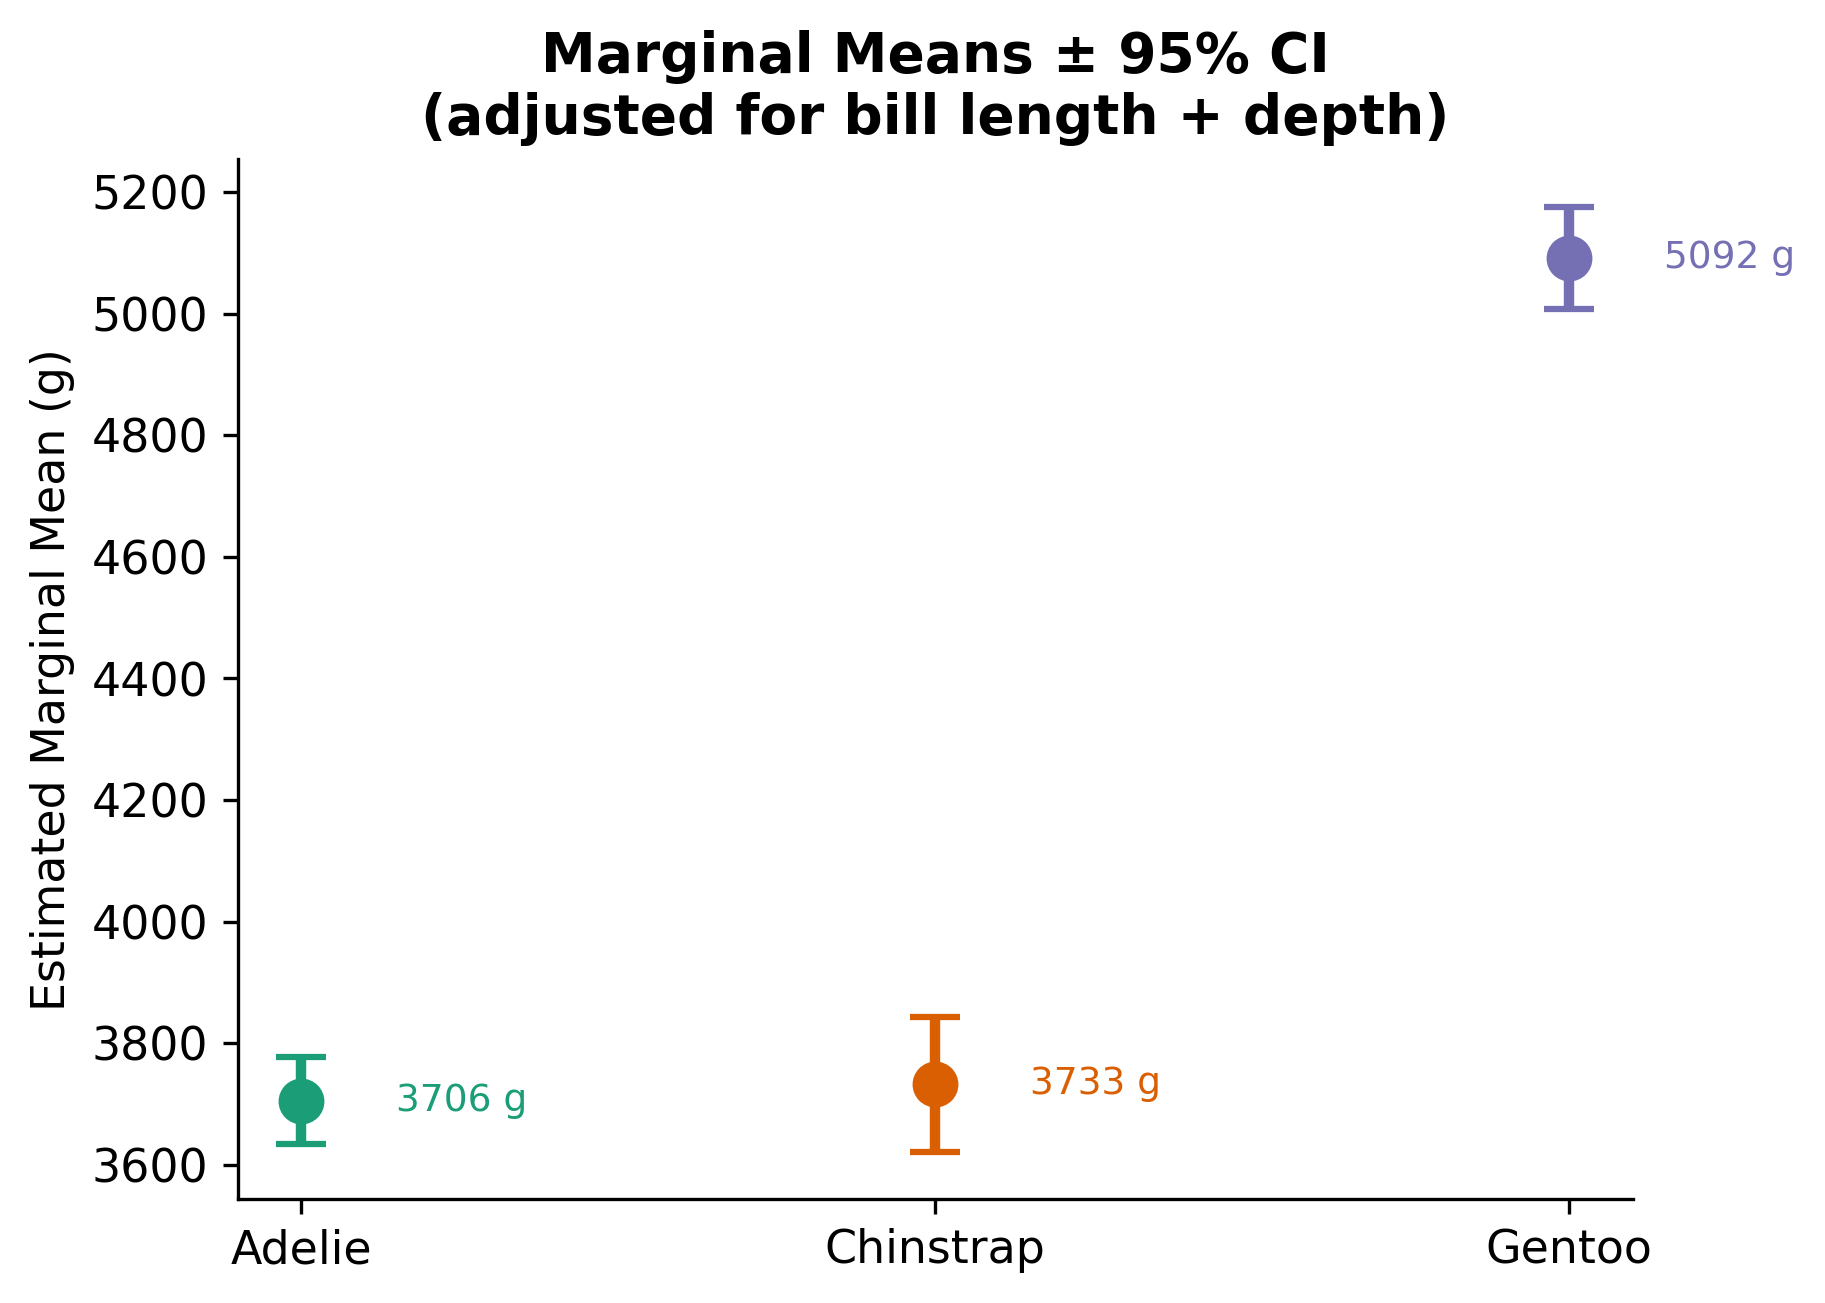
\includegraphics[width=\textwidth]{m2_5_marginal_means.png}
\begin{alertblock}{Pro-Tip}
    \scriptsize The Python \texttt{marginaleffects} package (Arel-Bundock, 2023) mirrors R's \texttt{marginaleffects} and provides \texttt{predictions()}, \texttt{comparisons()}, and \texttt{slopes()} --- the closest Python equivalent to \texttt{emmeans}.
\end{alertblock}
\end{column}
\end{columns}
\end{frame}

% ── 136 ──
\begin{frame}{Pairwise Contrasts}
\smark{136/300}
\centering
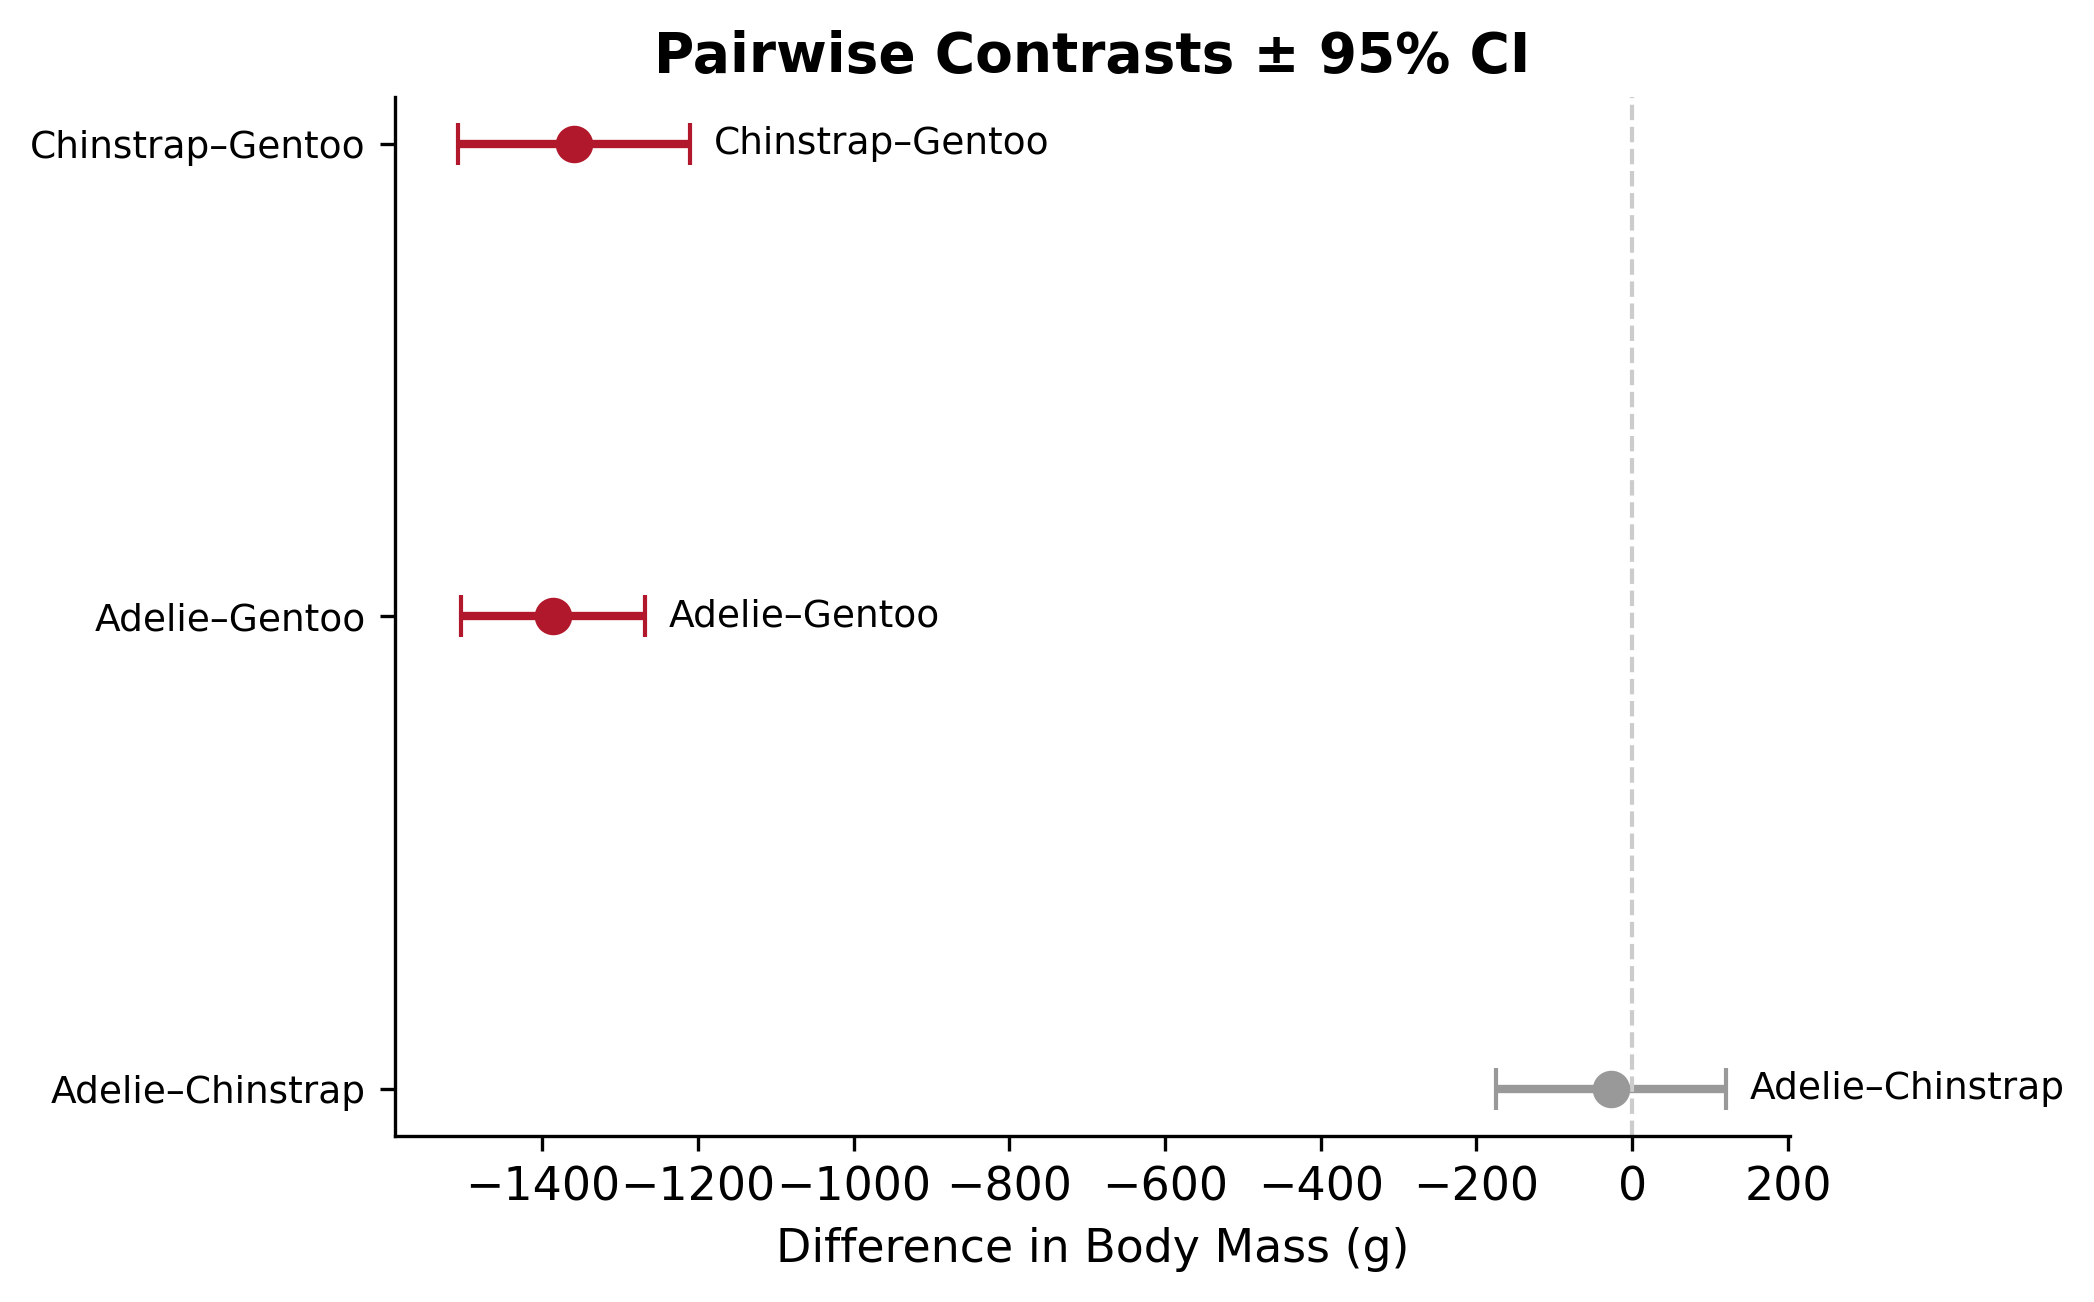
\includegraphics[width=0.62\textwidth]{m2_5_pairwise_contrasts.png}

\vspace{0.2cm}
\begin{columns}[T]
\begin{column}{0.48\textwidth}
\begin{itemize}
    \item Difference between each pair of group means
    \item CI of the difference $\to$ significance
    \item If CI includes zero $\to$ not significantly different
    \item Tukey HSD or Bonferroni adjustment for multiplicity
\end{itemize}
\end{column}
\begin{column}{0.48\textwidth}
\begin{exampleblock}{Data Insight}
    \scriptsize Adelie--Chinstrap CI crosses zero (grey): not significantly different. Both comparisons with Gentoo are far from zero (red): Gentoo is significantly heavier. The visual makes this instantly clear.
\end{exampleblock}
\end{column}
\end{columns}
\end{frame}

% ── 137 ──
\begin{frame}[fragile]{Pairwise Contrasts --- Code}\smark{137/300}
\begin{columns}[T]
\begin{column}{0.48\textwidth}
\begin{lstlisting}[style=Rstyle]
library(emmeans)

emm <- emmeans(model, ~ species)

# Pairwise comparisons
pairs(emm, adjust = "tukey")

# Plot contrasts
plot(pairs(emm)) +
  geom_vline(xintercept = 0,
    linetype = "dashed",
    color = "#B2182B") +
  theme_minimal()

# Compact letter display
cld(emm, adjust = "tukey",
    Letters = letters)
# a, b groups for significance
\end{lstlisting}
\end{column}
\begin{column}{0.48\textwidth}
\begin{lstlisting}[style=Pystyle]
# statsmodels Tukey HSD
from statsmodels.stats \
    .multicomp import pairwise_tukeyhsd

tukey = pairwise_tukeyhsd(
    penguins["body_mass_g"],
    penguins["species"],
    alpha=0.05)
print(tukey)
tukey.plot_simultaneous()

# marginaleffects comparisons
from marginaleffects import \
    comparisons
comp = comparisons(model,
    variables="species")
\end{lstlisting}
\vspace{0.1cm}
\begin{alertblock}{Pro-Tip}
    \scriptsize \texttt{pairwise\_tukeyhsd()} is the Python equivalent. Its \texttt{plot\_simultaneous()} method creates a forest-style contrast plot.
\end{alertblock}
\end{column}
\end{columns}
\end{frame}

% ── 138 ──
\begin{frame}{Effect Plots: Predicted Values Across Range}
\smark{138/300}
\centering
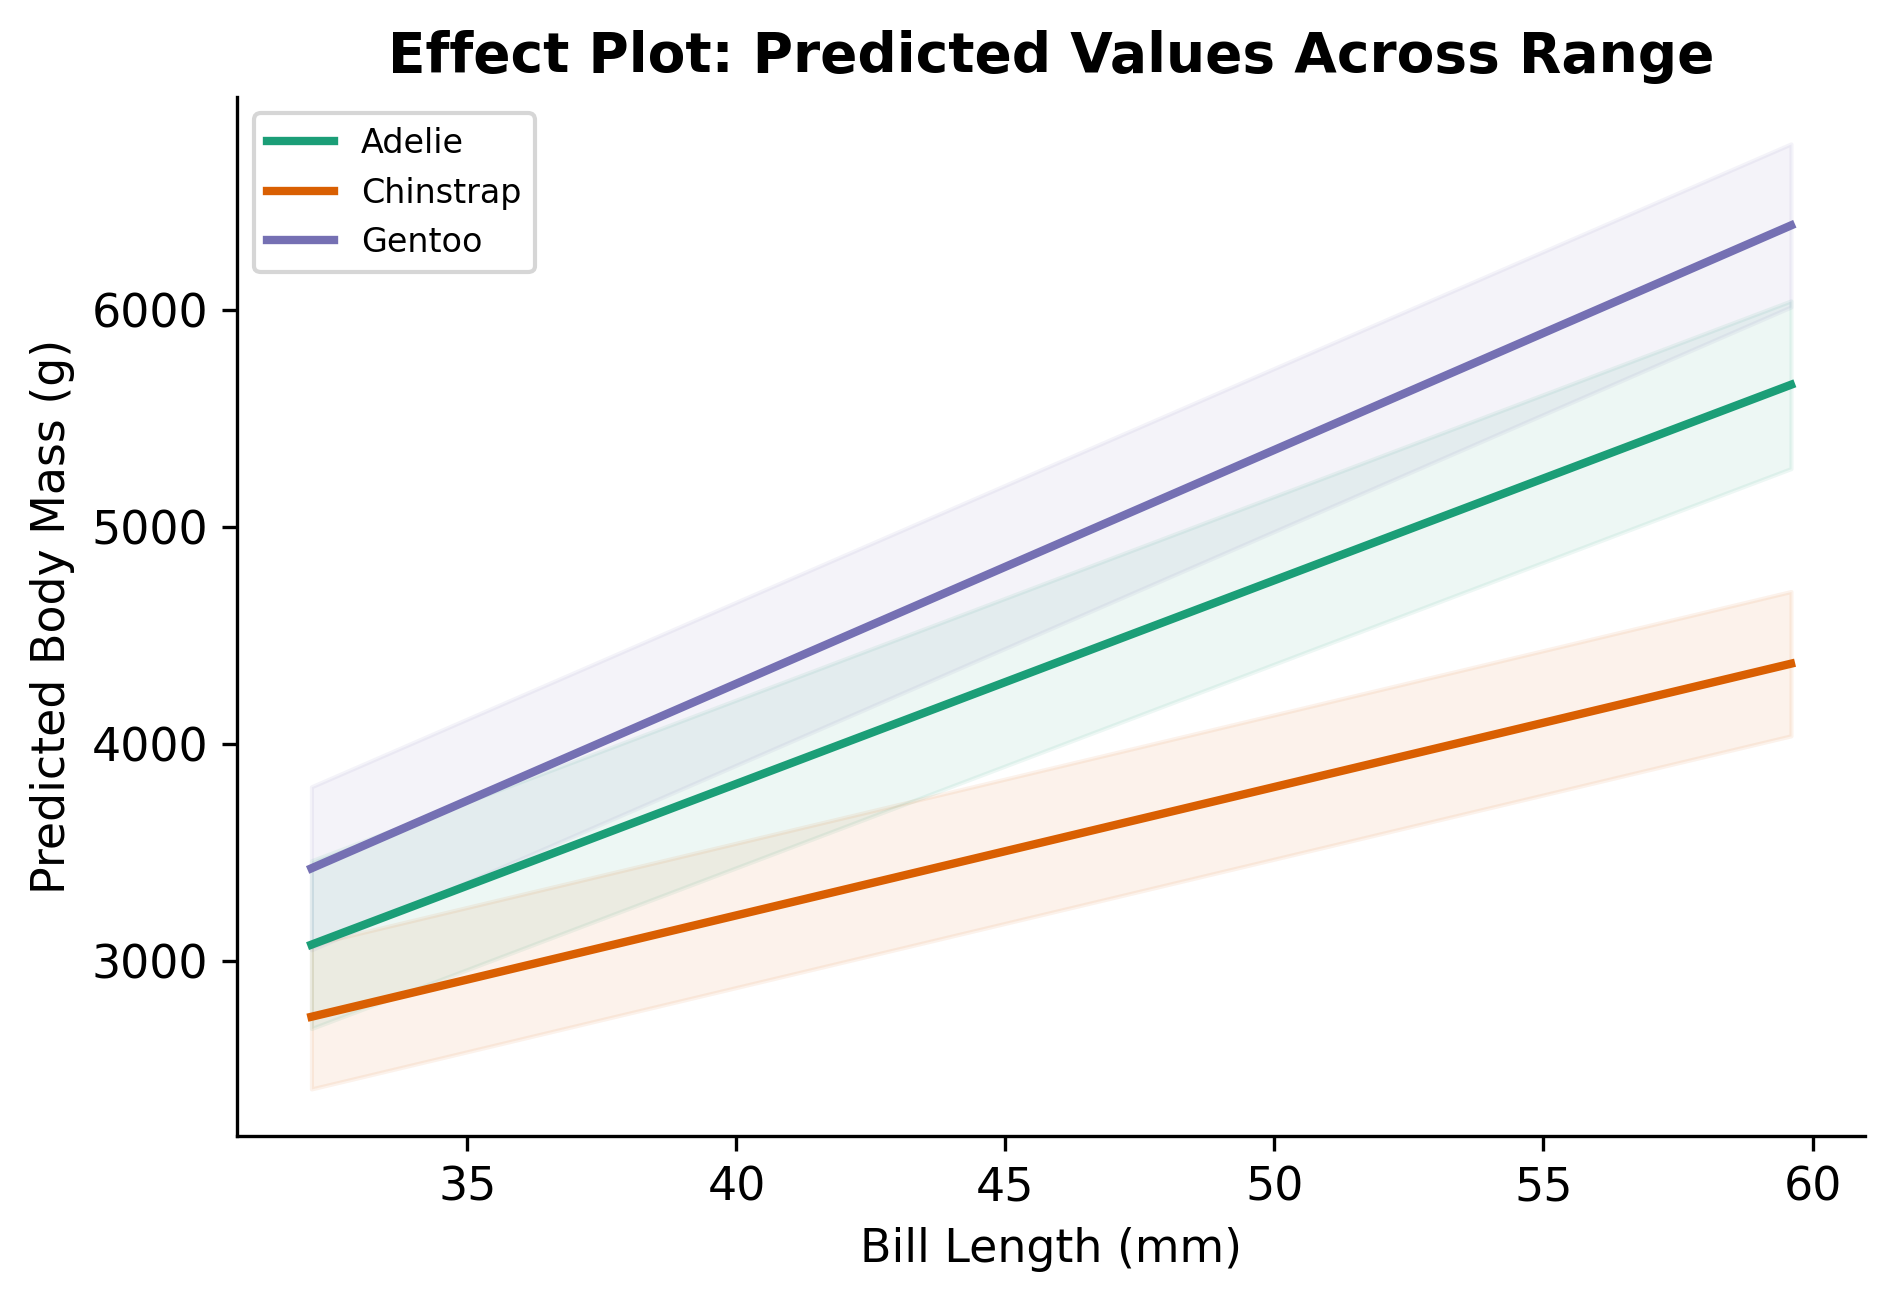
\includegraphics[width=0.68\textwidth]{m2_5_effect_plot.png}

\vspace{0.2cm}
\begin{columns}[T]
\begin{column}{0.48\textwidth}
\begin{itemize}
    \item Predicted $\hat{y}$ across the full range of a focal predictor
    \item Other predictors held at reference values (means or modes)
    \item Shows the \textbf{shape} of the predictor's effect
    \item CI band shows precision of the prediction
\end{itemize}
\end{column}
\begin{column}{0.48\textwidth}
\begin{exampleblock}{Data Insight}
    \scriptsize Effect plots are the best way to \textbf{communicate regression results} to non-statisticians. A coefficient of $\beta = 87$ g/mm is abstract; a line showing mass increasing from 3000 to 5500\,g across the bill-length range is tangible.
\end{exampleblock}
\end{column}
\end{columns}
\end{frame}

% ── 139 ──
\begin{frame}[fragile]{Effect Plot --- \Rlang}\smark{139/300}
\begin{columns}[T]
\begin{column}{0.55\textwidth}
\begin{lstlisting}[style=Rstyle]
# effects package
library(effects)
plot(allEffects(model))

# marginaleffects (modern)
library(marginaleffects)
plot_predictions(model,
  condition = "bill_length_mm",
  by = "species") +
  theme_minimal()

# Manual with predict()
grid <- expand.grid(
  bill_length_mm = seq(32,60,0.5),
  species = c("Adelie","Gentoo"),
  bill_depth_mm = mean(
    penguins$bill_depth_mm))
grid$pred <- predict(model, grid)
\end{lstlisting}
\end{column}
\begin{column}{0.42\textwidth}
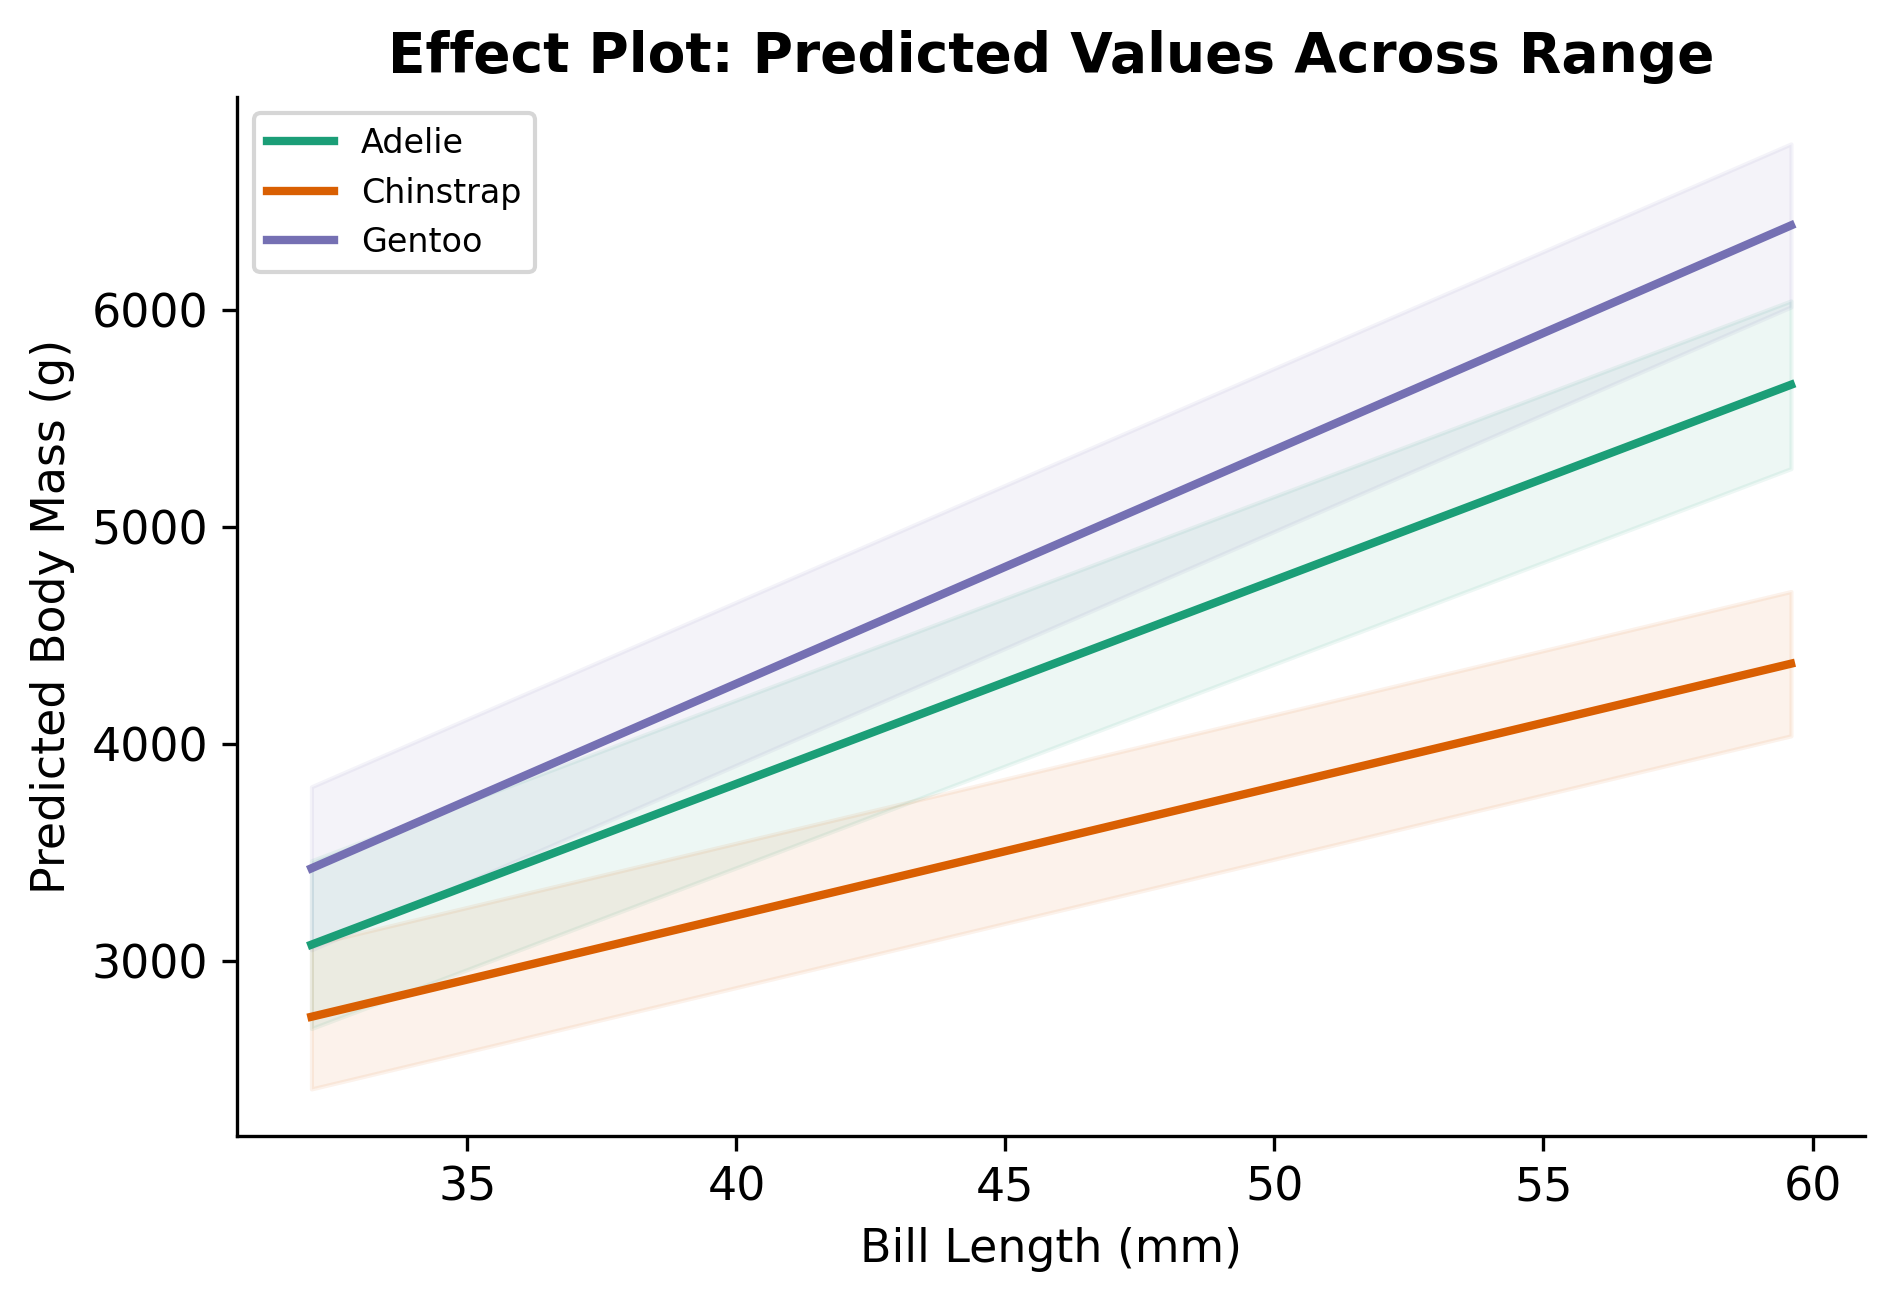
\includegraphics[width=\textwidth]{m2_5_effect_plot.png}
\begin{alertblock}{Pro-Tip}
    \scriptsize \texttt{marginaleffects::plot\_predictions()} is the modern replacement for \texttt{effects::plot(allEffects())}. It handles interactions, non-linear terms, and mixed models.
\end{alertblock}
\end{column}
\end{columns}
\end{frame}

% ── 140 ──
\begin{frame}[fragile]{Effect Plot --- \Python}\smark{140/300}
\begin{columns}[T]
\begin{column}{0.55\textwidth}
\begin{lstlisting}[style=Pystyle]
# marginaleffects
from marginaleffects import \
    plot_predictions
plot_predictions(model,
    condition=["bill_length_mm",
               "species"])

# Manual: prediction grid
bl_range = np.linspace(32, 60, 100)
for sp in species_list:
    grid = pd.DataFrame({
        "bill_length_mm": bl_range,
        "species": sp,
        "bill_depth_mm": bd_mean})
    X = build_design_matrix(grid)
    pred = model.get_prediction(X)
    ci = pred.summary_frame()
    ax.plot(bl_range, ci["mean"],
        label=sp)
    ax.fill_between(bl_range,
        ci["mean_ci_lower"],
        ci["mean_ci_upper"],
        alpha=0.12)
\end{lstlisting}
\end{column}
\begin{column}{0.42\textwidth}
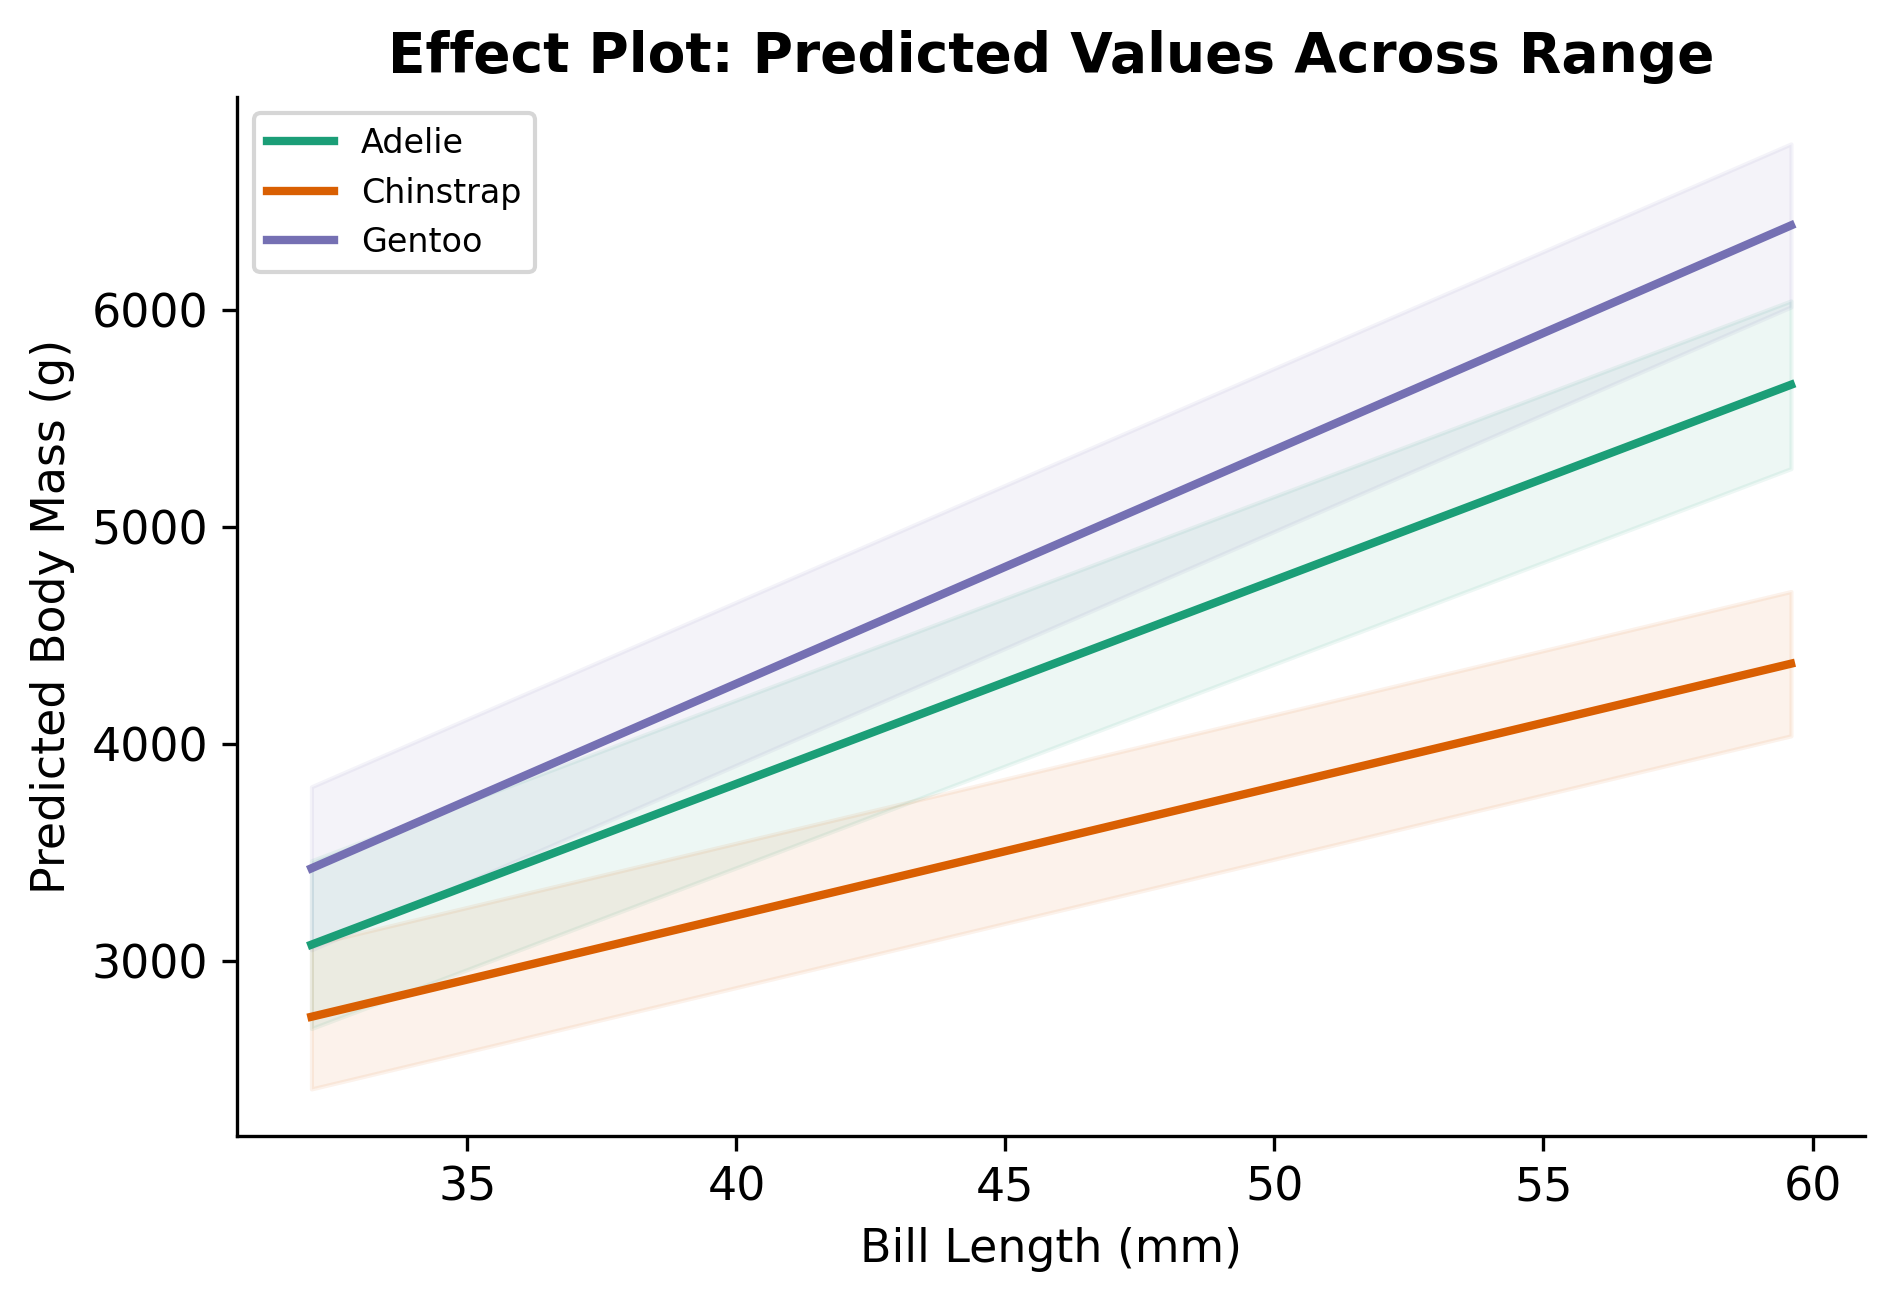
\includegraphics[width=\textwidth]{m2_5_effect_plot.png}
\end{column}
\end{columns}
\end{frame}

% ── 141 ──
\begin{frame}{Model Predictions vs.\ Raw Data}
\smark{141/300}
\begin{columns}[T]
\begin{column}{0.50\textwidth}
\begin{itemize}
    \item Always overlay model predictions on raw data
    \item Predictions alone can mask poor fit
    \item Raw data alone misses the model's message
    \item The combination is the \textbf{complete story}
\end{itemize}
\end{column}
\begin{column}{0.47\textwidth}
\begin{alertblock}{Pro-Tip}
    \scriptsize Recipe: (1) scatter raw data in light alpha; (2) overlay model fit as a solid line; (3) add CI band. This is what \texttt{geom\_smooth()} does internally --- but you can do it from any fitted model.
\end{alertblock}
\vspace{0.1cm}
\begin{exampleblock}{Data Insight}
    \scriptsize If the model line misses systematic clusters of raw data, the model is \textbf{mis-specified}. Visual comparison catches problems that $R^2$ alone cannot.
\end{exampleblock}
\end{column}
\end{columns}
\end{frame}

% ── 142 ──
\begin{frame}[fragile]{Predictions + Raw Data --- Code}\smark{142/300}
\begin{columns}[T]
\begin{column}{0.48\textwidth}
\begin{lstlisting}[style=Rstyle]
# Raw data + model fit
ggplot(penguins,
  aes(bill_length_mm,
      body_mass_g,
      color = species)) +
  # Raw data (light)
  geom_point(alpha = 0.3) +
  # Model predictions
  geom_smooth(method = "lm",
    se = TRUE) +
  theme_minimal()

# From fitted model explicitly
grid$pred <- predict(model, grid,
  interval="confidence")
ggplot() +
  geom_point(data=penguins, ...,
    alpha=0.2) +
  geom_line(data=grid, aes(y=fit))+
  geom_ribbon(data=grid, ...)
\end{lstlisting}
\end{column}
\begin{column}{0.48\textwidth}
\begin{lstlisting}[style=Pystyle]
# seaborn: raw + regression
fig, ax = plt.subplots()
sns.scatterplot(data=penguins,
    x="bill_length_mm",
    y="body_mass_g",
    hue="species", alpha=0.3,
    ax=ax)
# Add model predictions
for sp, c in zip(species, colors):
    ax.plot(grid_x, pred_y,
        color=c, linewidth=2)
    ax.fill_between(grid_x,
        ci_lo, ci_hi,
        alpha=0.12, color=c)
\end{lstlisting}
\end{column}
\end{columns}
\end{frame}

% ── 143 ──
\begin{frame}{The \texttt{marginaleffects} Ecosystem}
\smark{143/300}
\centering\small
\begin{tabular}{@{}lll@{}}
    \toprule
    \textbf{Function} & \textbf{R} & \textbf{Python} \\
    \midrule
    Predicted values    & \texttt{predictions()}     & \texttt{predictions()} \\
    Marginal effects    & \texttt{slopes()}          & \texttt{slopes()} \\
    Contrasts           & \texttt{comparisons()}     & \texttt{comparisons()} \\
    Plot predictions    & \texttt{plot\_predictions()} & \texttt{plot\_predictions()} \\
    Plot slopes         & \texttt{plot\_slopes()}      & \texttt{plot\_slopes()} \\
    Plot comparisons    & \texttt{plot\_comparisons()} & \texttt{plot\_comparisons()} \\
    \bottomrule
\end{tabular}

\vspace{0.3cm}
\begin{exampleblock}{Data Insight}
    \scriptsize The \texttt{marginaleffects} package (Arel-Bundock) is the unified interface for model interpretation in both R and Python. It replaces \texttt{emmeans}, \texttt{effects}, and \texttt{ggeffects} for most use cases.
\end{exampleblock}
\end{frame}

% ── 144 ──
\begin{frame}{Conditional Effects: Spotlight Analysis}
\smark{144/300}
\begin{columns}[T]
\begin{column}{0.50\textwidth}
\begin{itemize}
    \item When a continuous $\times$ continuous interaction exists
    \item ``Spotlight'' the effect of $x_1$ at specific values of $x_2$ (e.g., mean, $\pm 1$ SD)
    \item Produces 3 regression lines: one per level of the moderator
    \item Johnson--Neyman interval: the range of $x_2$ where the effect of $x_1$ is significant
\end{itemize}
\end{column}
\begin{column}{0.47\textwidth}
\begin{alertblock}{Pro-Tip}
    \scriptsize R: \texttt{marginaleffects::plot\_slopes(model, variables="x1", condition="x2")} with \texttt{x2} at chosen values. \texttt{interactions::interact\_plot()} is another clean option.
\end{alertblock}
\vspace{0.1cm}
\begin{exampleblock}{Data Insight}
    \scriptsize The Johnson--Neyman plot (\texttt{interactions::johnson\_neyman()}) shades the region where the effect is significant. Points outside the shaded region have non-significant slopes.
\end{exampleblock}
\end{column}
\end{columns}
\end{frame}

% ── 145 ──
\begin{frame}[fragile]{Spotlight / Johnson--Neyman --- Code}\smark{145/300}
\begin{columns}[T]
\begin{column}{0.48\textwidth}
\begin{lstlisting}[style=Rstyle]
library(interactions)

model <- lm(body_mass_g ~
  bill_length_mm * bill_depth_mm,
  data = penguins)

# Spotlight at -1SD, mean, +1SD
interact_plot(model,
  pred = bill_length_mm,
  modx = bill_depth_mm,
  modx.values = "plus-minus",
  plot.points = TRUE,
  point.alpha = 0.2)

# Johnson-Neyman interval
johnson_neyman(model,
  pred = bill_length_mm,
  modx = bill_depth_mm)
\end{lstlisting}
\end{column}
\begin{column}{0.48\textwidth}
\begin{lstlisting}[style=Pystyle]
# Manual spotlight in Python
moderator_vals = [
    bd_mean - bd_sd,
    bd_mean,
    bd_mean + bd_sd]

for mod_val, ls in zip(
    moderator_vals,
    ["-1 SD","Mean","+1 SD"]):
    grid = pd.DataFrame({
        "bill_length_mm": bl_range,
        "bill_depth_mm": mod_val})
    X = build_matrix(grid)
    pred = model.get_prediction(X)
    ax.plot(bl_range,
        pred.predicted_mean,
        label=f"Depth = {ls}")
ax.legend()
\end{lstlisting}
\end{column}
\end{columns}
\end{frame}

% ── 146 ──
\begin{frame}{Three-Way Interactions: Faceted Interaction Plots}
\smark{146/300}
\begin{columns}[T]
\begin{column}{0.50\textwidth}
\begin{itemize}
    \item Three-way: effect of $x$ depends on $g_1$ \textbf{and} $g_2$
    \item Visualization: facet by $g_2$, color by $g_1$, plot lines
    \item Each panel shows a 2-way interaction at a fixed level of $g_2$
    \item If the interaction pattern \textbf{differs across panels}, the 3-way is present
\end{itemize}
\end{column}
\begin{column}{0.47\textwidth}
\begin{alertblock}{Pro-Tip}
    \scriptsize R: \texttt{emmip(model, sex \textasciitilde\ species | island)}. The \texttt{|} operator facets by island. In Python: loop over levels of the third variable and create subplots.
\end{alertblock}
\vspace{0.1cm}
\begin{exampleblock}{Data Insight}
    \scriptsize Three-way interactions are hard to interpret in tables (8+ coefficients). The faceted interaction plot makes the pattern graspable in seconds.
\end{exampleblock}
\end{column}
\end{columns}
\end{frame}

% ── 147 ──
\begin{frame}[fragile]{Three-Way Interaction --- Code}\smark{147/300}
\begin{columns}[T]
\begin{column}{0.48\textwidth}
\begin{lstlisting}[style=Rstyle]
model <- lm(body_mass_g ~
  bill_length_mm * species * sex,
  data = penguins)

# Faceted interaction plot
library(emmeans)
emmip(model,
  sex ~ species | island,
  CIs = TRUE) +
  theme_minimal()

# Or with marginaleffects
plot_predictions(model,
  condition = c("species",
    "sex", "island"))
\end{lstlisting}
\end{column}
\begin{column}{0.48\textwidth}
\begin{lstlisting}[style=Pystyle]
# seaborn catplot with facet
sns.catplot(data=penguins,
    x="species", y="body_mass_g",
    hue="sex", col="island",
    kind="point",
    errorbar="se",
    capsize=0.1,
    height=3.5, aspect=0.9)

# marginaleffects
from marginaleffects import \
    plot_predictions
plot_predictions(model,
    condition=["species","sex"],
    by="island")
\end{lstlisting}
\end{column}
\end{columns}
\end{frame}

% ── 148 ──
\begin{frame}{Marginal Effects at Representative Values (MER)}
\smark{148/300}
\begin{columns}[T]
\begin{column}{0.50\textwidth}
\begin{itemize}
    \item For non-linear models (logistic, Poisson), coefficients are not directly interpretable
    \item \textbf{Marginal effects}: $\partial \hat{y} / \partial x$ evaluated at specific values
    \item \textbf{AME}: average marginal effect (averaged over all observations)
    \item \textbf{MER}: marginal effect at representative values (e.g., median)
\end{itemize}
\end{column}
\begin{column}{0.47\textwidth}
\begin{exampleblock}{Data Insight}
    \scriptsize In logistic regression, $\beta = 0.5$ means a 0.5 increase in log-odds per unit $x$. The marginal effect in \emph{probability} depends on where you are on the sigmoid. Plotting the predicted probability curve is more honest than reporting a single number.
\end{exampleblock}
\end{column}
\end{columns}
\end{frame}

% ── 149 ──
\begin{frame}[fragile]{Marginal Effects for GLMs --- Code}\smark{149/300}
\begin{columns}[T]
\begin{column}{0.48\textwidth}
\begin{lstlisting}[style=Rstyle]
library(marginaleffects)

glm_model <- glm(survived ~
  age * sex + class,
  family=binomial, data=titanic)

# Average marginal effects
avg_slopes(glm_model)

# Plot predicted probability
plot_predictions(glm_model,
  condition = c("age","sex")) +
  theme_minimal()

# Marginal effect of age
plot_slopes(glm_model,
  variables = "age",
  condition = "sex")
\end{lstlisting}
\end{column}
\begin{column}{0.48\textwidth}
\begin{lstlisting}[style=Pystyle]
from marginaleffects import (
    avg_slopes, plot_predictions,
    plot_slopes)

# Average marginal effects
avg_slopes(glm_model)

# Plot predicted probability
plot_predictions(glm_model,
    condition=["age","sex"])

# Marginal effect of age
plot_slopes(glm_model,
    variables="age",
    condition="sex")
\end{lstlisting}
\vspace{0.1cm}
\begin{alertblock}{Pro-Tip}
    \scriptsize For logistic regression, always plot predictions on the \textbf{probability scale} (not log-odds). \texttt{plot\_predictions()} does this automatically.
\end{alertblock}
\end{column}
\end{columns}
\end{frame}

% ── 150 ──
\begin{frame}{Module 2.5 --- Key Takeaways}\smark{150/300}
\begin{enumerate}
    \item \textbf{Non-parallel slopes = interaction.} Visual test first, then formal.
    \item \textbf{Simpson's paradox} reverses effects when a confound is ignored. Always color by group.
    \item \textbf{Interaction plots}: lines for cat $\times$ cat; separate regression lines for cont $\times$ cat.
    \item \textbf{emmeans} give model-adjusted means --- not raw sample means.
    \item \textbf{Pairwise contrasts} with CIs replace stars and $p$-values.
    \item \textbf{Effect plots} translate regression coefficients into human-readable predictions.
\end{enumerate}
\end{frame}

% ── 151 ──
\begin{frame}{}\smark{151/300}
\centering\vspace{1.5cm}
{\Large\textbf{Module 2.5 Complete}}\\[0.5cm]
You can now visualize interactions, Simpson's paradox, marginal means, pairwise contrasts, and model-predicted effects --- turning regression tables into intuitive graphics.\\[0.5cm]
\textbf{Next:} Module 2.6 --- Correlation, Association, and Heatmaps.
\end{frame}

% % ═══════════════════════════════════════════════════════
%  MODULE 2.6 — Correlation, Association, and Heatmaps
% ═══════════════════════════════════════════════════════
\section{Module 2.6 --- Correlation, Association, and Heatmaps}

% ── 152 ──
\begin{frame}{Module 2.6 --- Roadmap}\smark{152/300}
\begin{enumerate}
    \item Pearson, Spearman, Kendall: when to use which
    \item Correlation matrix heatmap
    \item Lower-triangle masking and annotation
    \item Scatterplot matrix (pairs plot)
    \item Bubble correlograms
    \item Grouped correlations: faceted by category
    \item Aggregated heatmaps (cross-tabulated means)
    \item Correlation $\neq$ causation: visual caveats
\end{enumerate}
\end{frame}

% ── 153 ──
\begin{frame}{Pearson, Spearman, Kendall}
\smark{153/300}
\centering\small
\begin{tabular}{@{}llll@{}}
    \toprule
    \textbf{Coefficient} & \textbf{Measures} & \textbf{Assumes} & \textbf{Use When} \\
    \midrule
    Pearson $r$   & Linear association       & Normality, no outliers & Both continuous, linear \\
    Spearman $\rho$ & Monotonic association  & Ranks, no outliers     & Ordinal or non-linear monotone \\
    Kendall $\tau$  & Concordance of pairs   & Ranks                  & Small $n$, many ties \\
    \bottomrule
\end{tabular}

\vspace{0.3cm}
\begin{columns}[T]
\begin{column}{0.48\textwidth}
\begin{alertblock}{Pro-Tip}
    \scriptsize Default to Pearson for exploration. Switch to Spearman if you see outliers or non-linearity in the scatter. Kendall for small ordinal datasets.
\end{alertblock}
\end{column}
\begin{column}{0.48\textwidth}
\begin{exampleblock}{Data Insight}
    \scriptsize $r = 0.87$ (flipper $\leftrightarrow$ mass) is strong linear. $r = -0.23$ (bill length $\leftrightarrow$ bill depth) is weak --- but within species it reverses (Simpson's paradox, Module 2.5).
\end{exampleblock}
\end{column}
\end{columns}
\end{frame}

% ── 154 ──
\begin{frame}{Correlation Matrix Heatmap}
\smark{154/300}
\centering
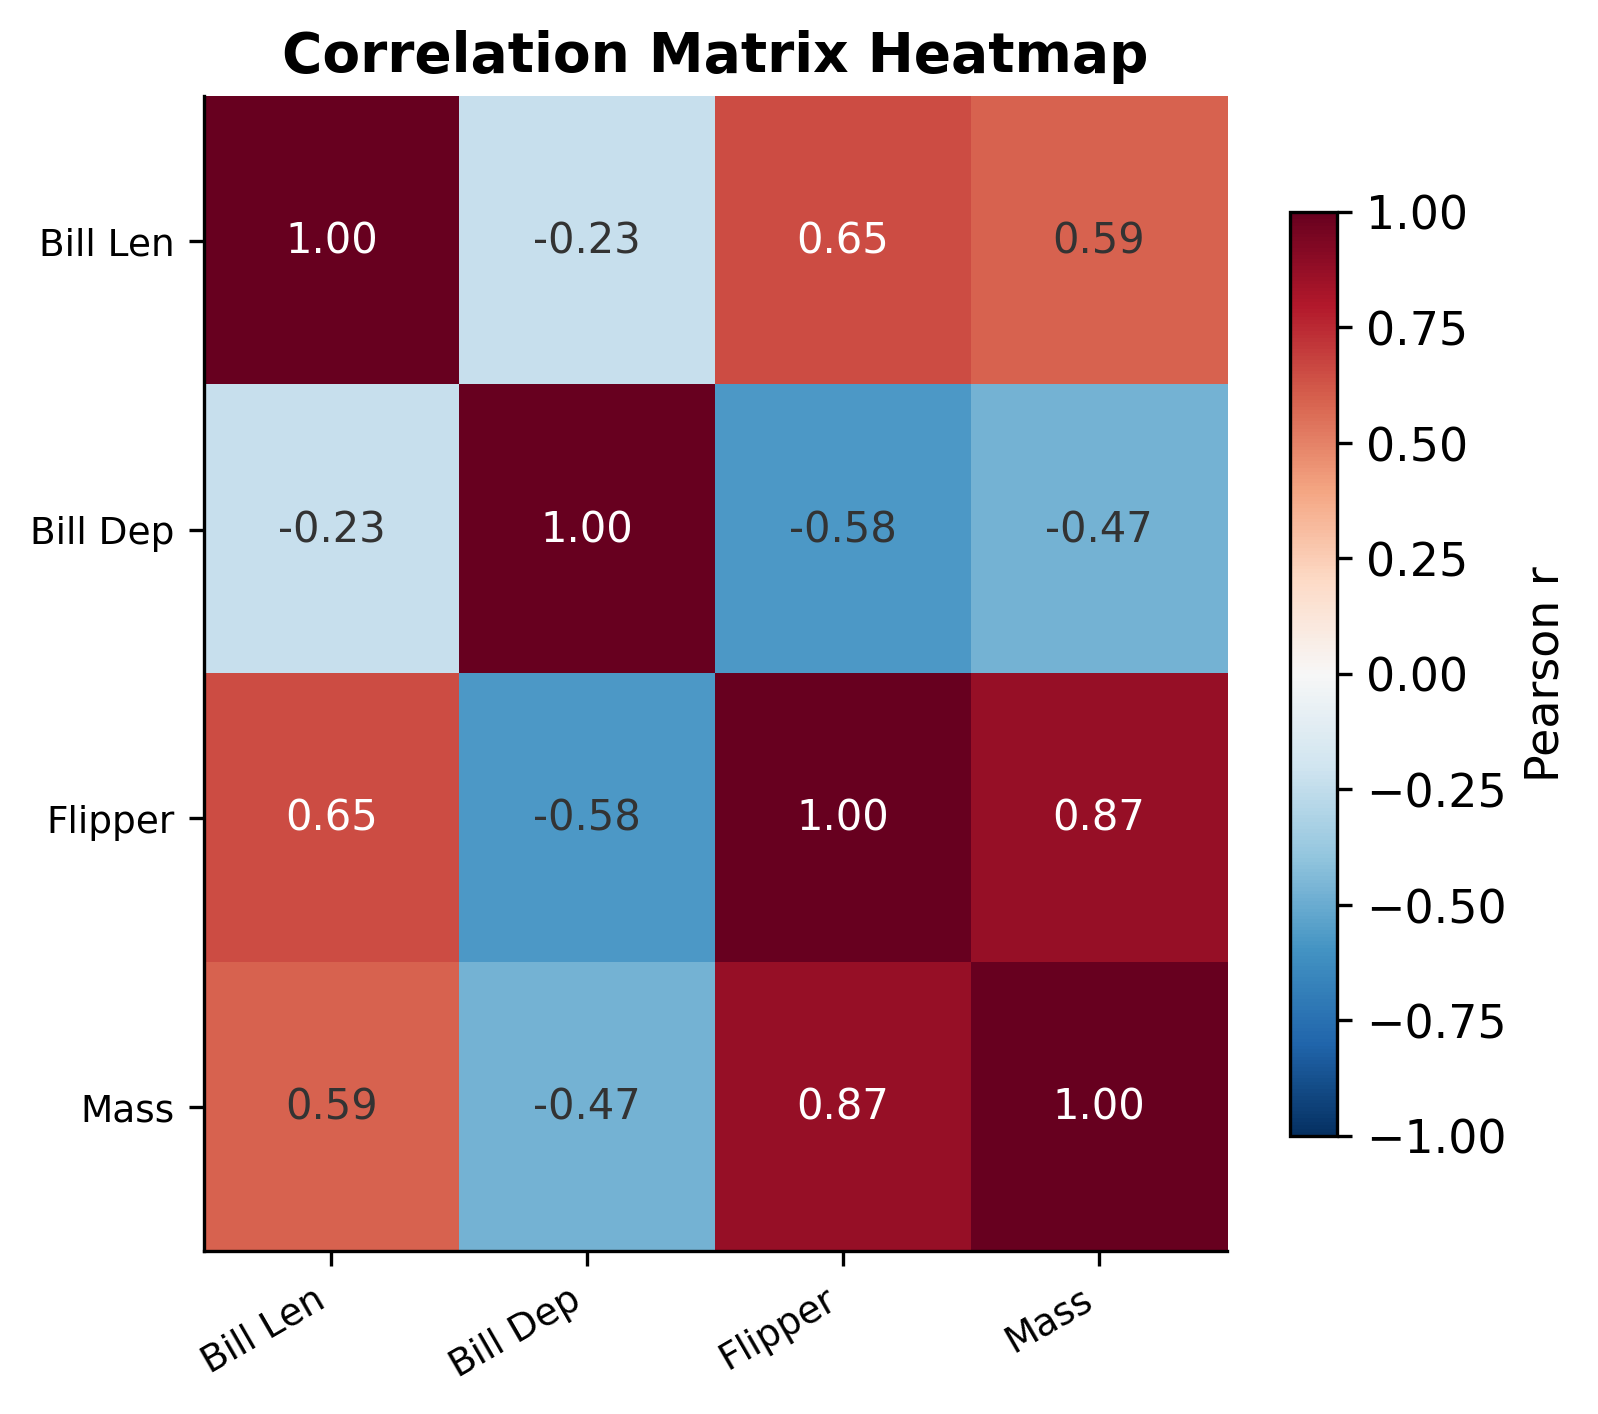
\includegraphics[width=0.55\textwidth]{m2_6_corr_heatmap.png}

\vspace{0.2cm}
\begin{columns}[T]
\begin{column}{0.48\textwidth}
\begin{itemize}
    \item Color encodes sign and magnitude
    \item Diverging palette (RdBu): red = negative, blue = positive
    \item Annotate cells with numeric $r$ values
    \item Diagonal is always 1.00
\end{itemize}
\end{column}
\begin{column}{0.48\textwidth}
\begin{alertblock}{Pro-Tip}
    \scriptsize Always use a \textbf{diverging} palette centered at zero. Sequential palettes (e.g., Blues) cannot distinguish positive from negative correlations.
\end{alertblock}
\end{column}
\end{columns}
\end{frame}

% ── 155 ──
\begin{frame}[fragile]{Correlation Heatmap --- \Rlang}\smark{155/300}
\begin{columns}[T]
\begin{column}{0.55\textwidth}
\begin{lstlisting}[style=Rstyle]
library(ggplot2)
library(reshape2)  # or tidyr

corr <- cor(penguins[, num_cols],
            use = "complete.obs")
melted <- melt(corr)

ggplot(melted,
  aes(Var1, Var2, fill=value)) +
  geom_tile(color="white") +
  geom_text(aes(label=
    sprintf("%.2f", value)),
    size=3.5) +
  scale_fill_gradient2(
    low="#B2182B", mid="white",
    high="#2166AC", midpoint=0,
    limits=c(-1,1)) +
  theme_minimal() +
  theme(axis.text.x =
    element_text(angle=30,
                 hjust=1))
\end{lstlisting}
\end{column}
\begin{column}{0.42\textwidth}
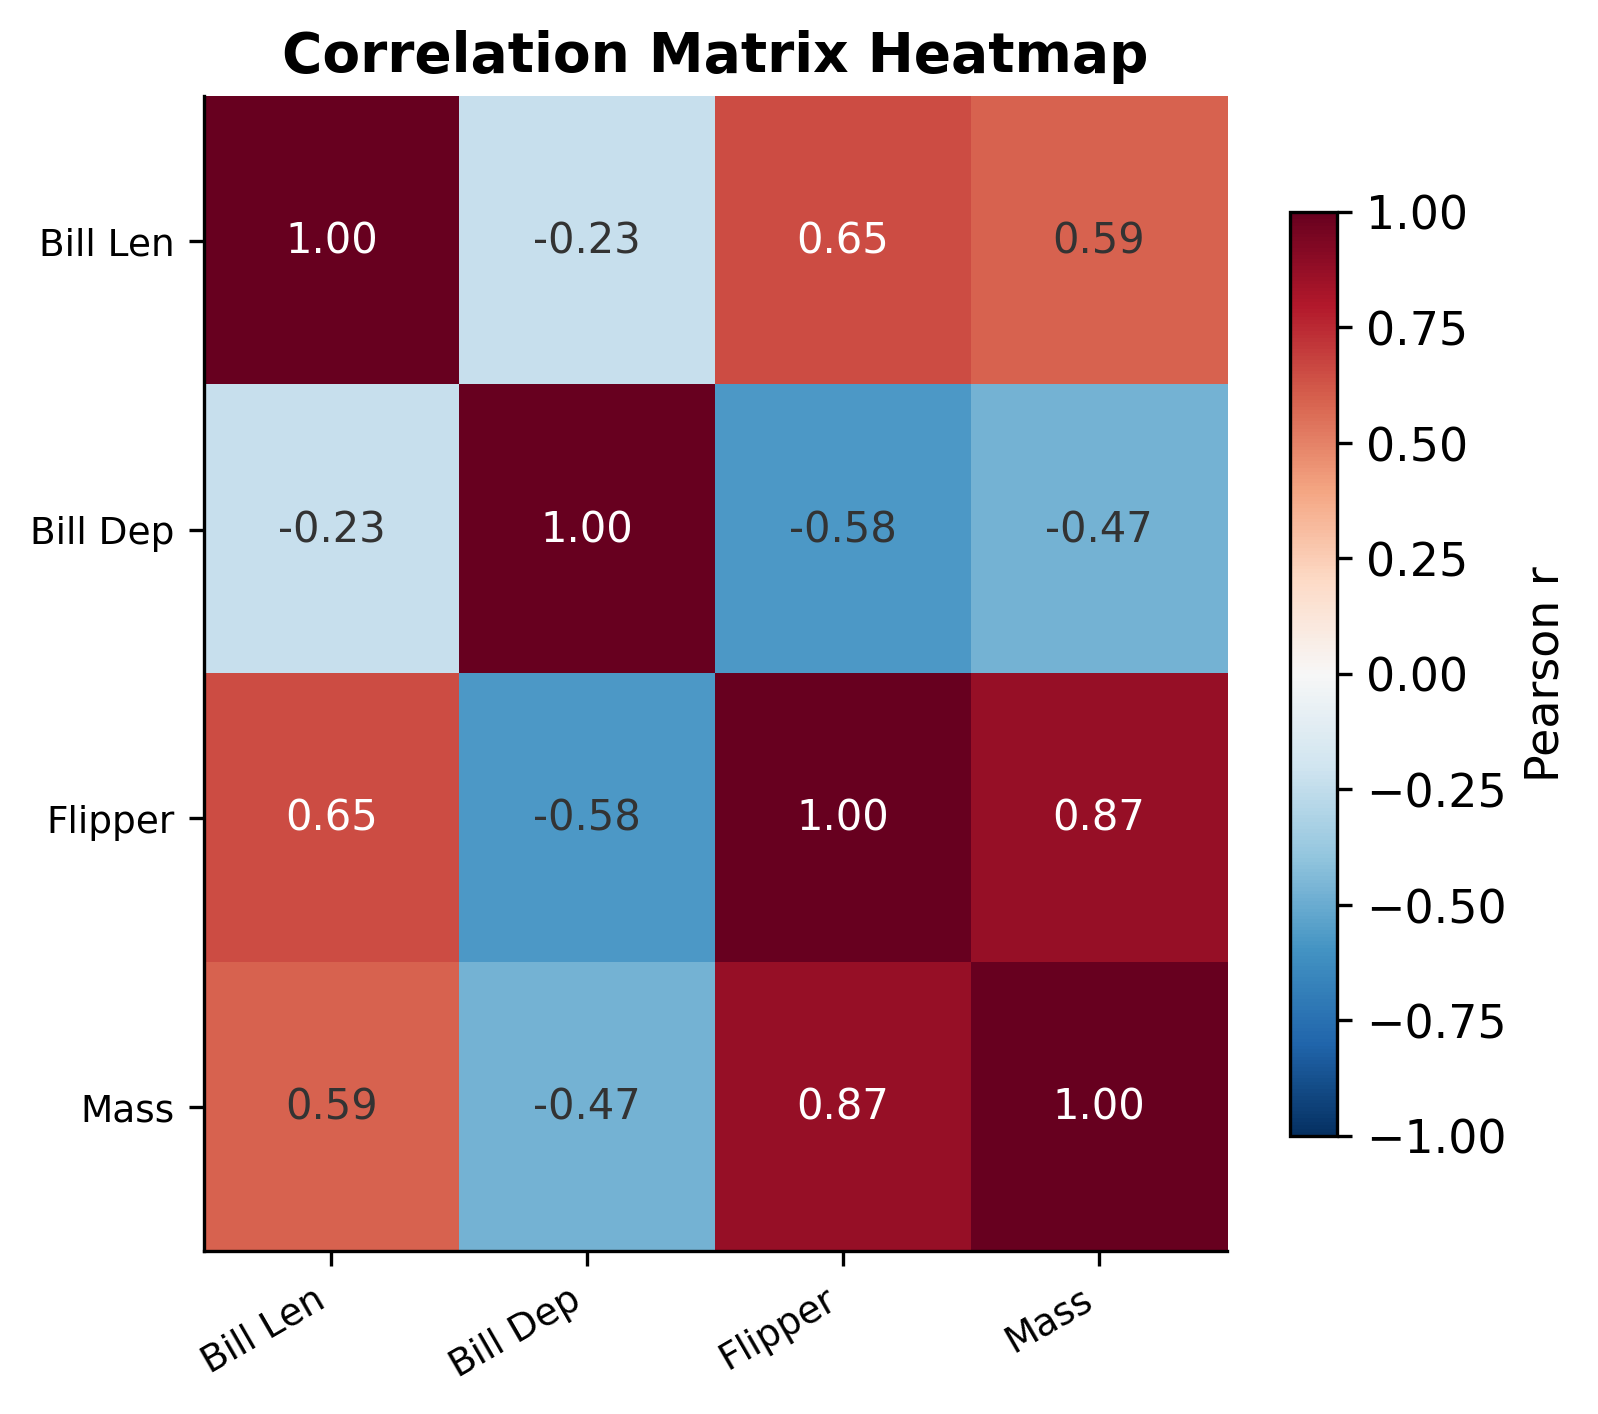
\includegraphics[width=\textwidth]{m2_6_corr_heatmap.png}
\begin{exampleblock}{Data Insight}
    \scriptsize \texttt{scale\_fill\_gradient2(midpoint=0)} centers the palette at zero. This is essential --- without it, the color scale is anchored at the data range and the midpoint drifts.
\end{exampleblock}
\end{column}
\end{columns}
\end{frame}

% ── 156 ──
\begin{frame}[fragile]{Correlation Heatmap --- \Python}\smark{156/300}
\begin{columns}[T]
\begin{column}{0.55\textwidth}
\begin{lstlisting}[style=Pystyle]
# seaborn (one-liner)
corr = penguins[num_cols].corr()
sns.heatmap(corr,
    annot=True, fmt=".2f",
    cmap="RdBu_r",
    vmin=-1, vmax=1,
    center=0,
    square=True,
    linewidths=0.5)

# Lower triangle only
mask = np.triu(
    np.ones_like(corr, dtype=bool))
sns.heatmap(corr,
    mask=mask, annot=True,
    fmt=".2f", cmap="RdBu_r",
    vmin=-1, vmax=1, center=0)
\end{lstlisting}
\end{column}
\begin{column}{0.42\textwidth}
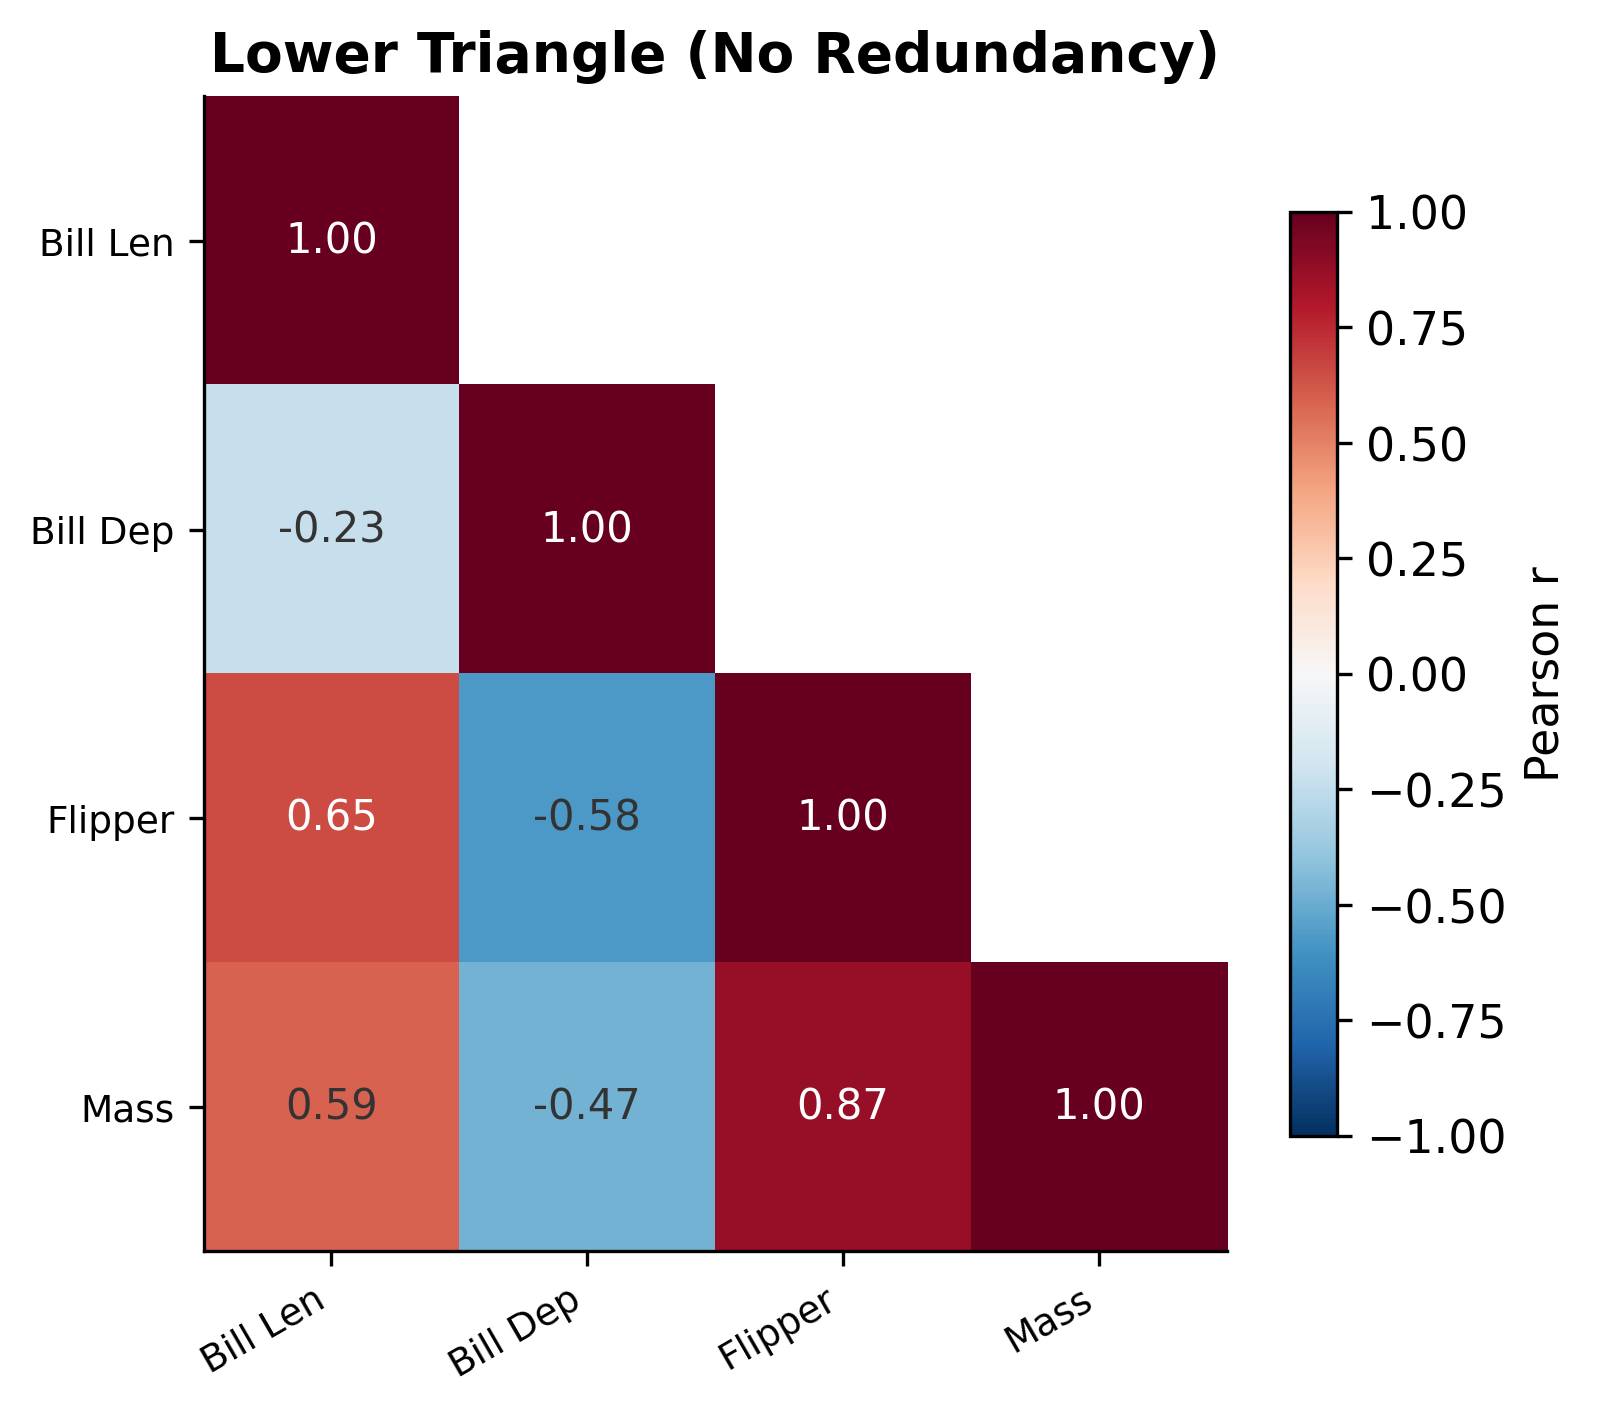
\includegraphics[width=\textwidth]{m2_6_corr_lower.png}
\begin{alertblock}{Pro-Tip}
    \scriptsize \texttt{sns.heatmap(mask=mask)} hides the upper triangle. The full matrix is symmetric, so the upper half is redundant. Masking saves ink and reduces visual clutter.
\end{alertblock}
\end{column}
\end{columns}
\end{frame}

% ── 157 ──
\begin{frame}{Lower Triangle: Removing Redundancy}
\smark{157/300}
\centering
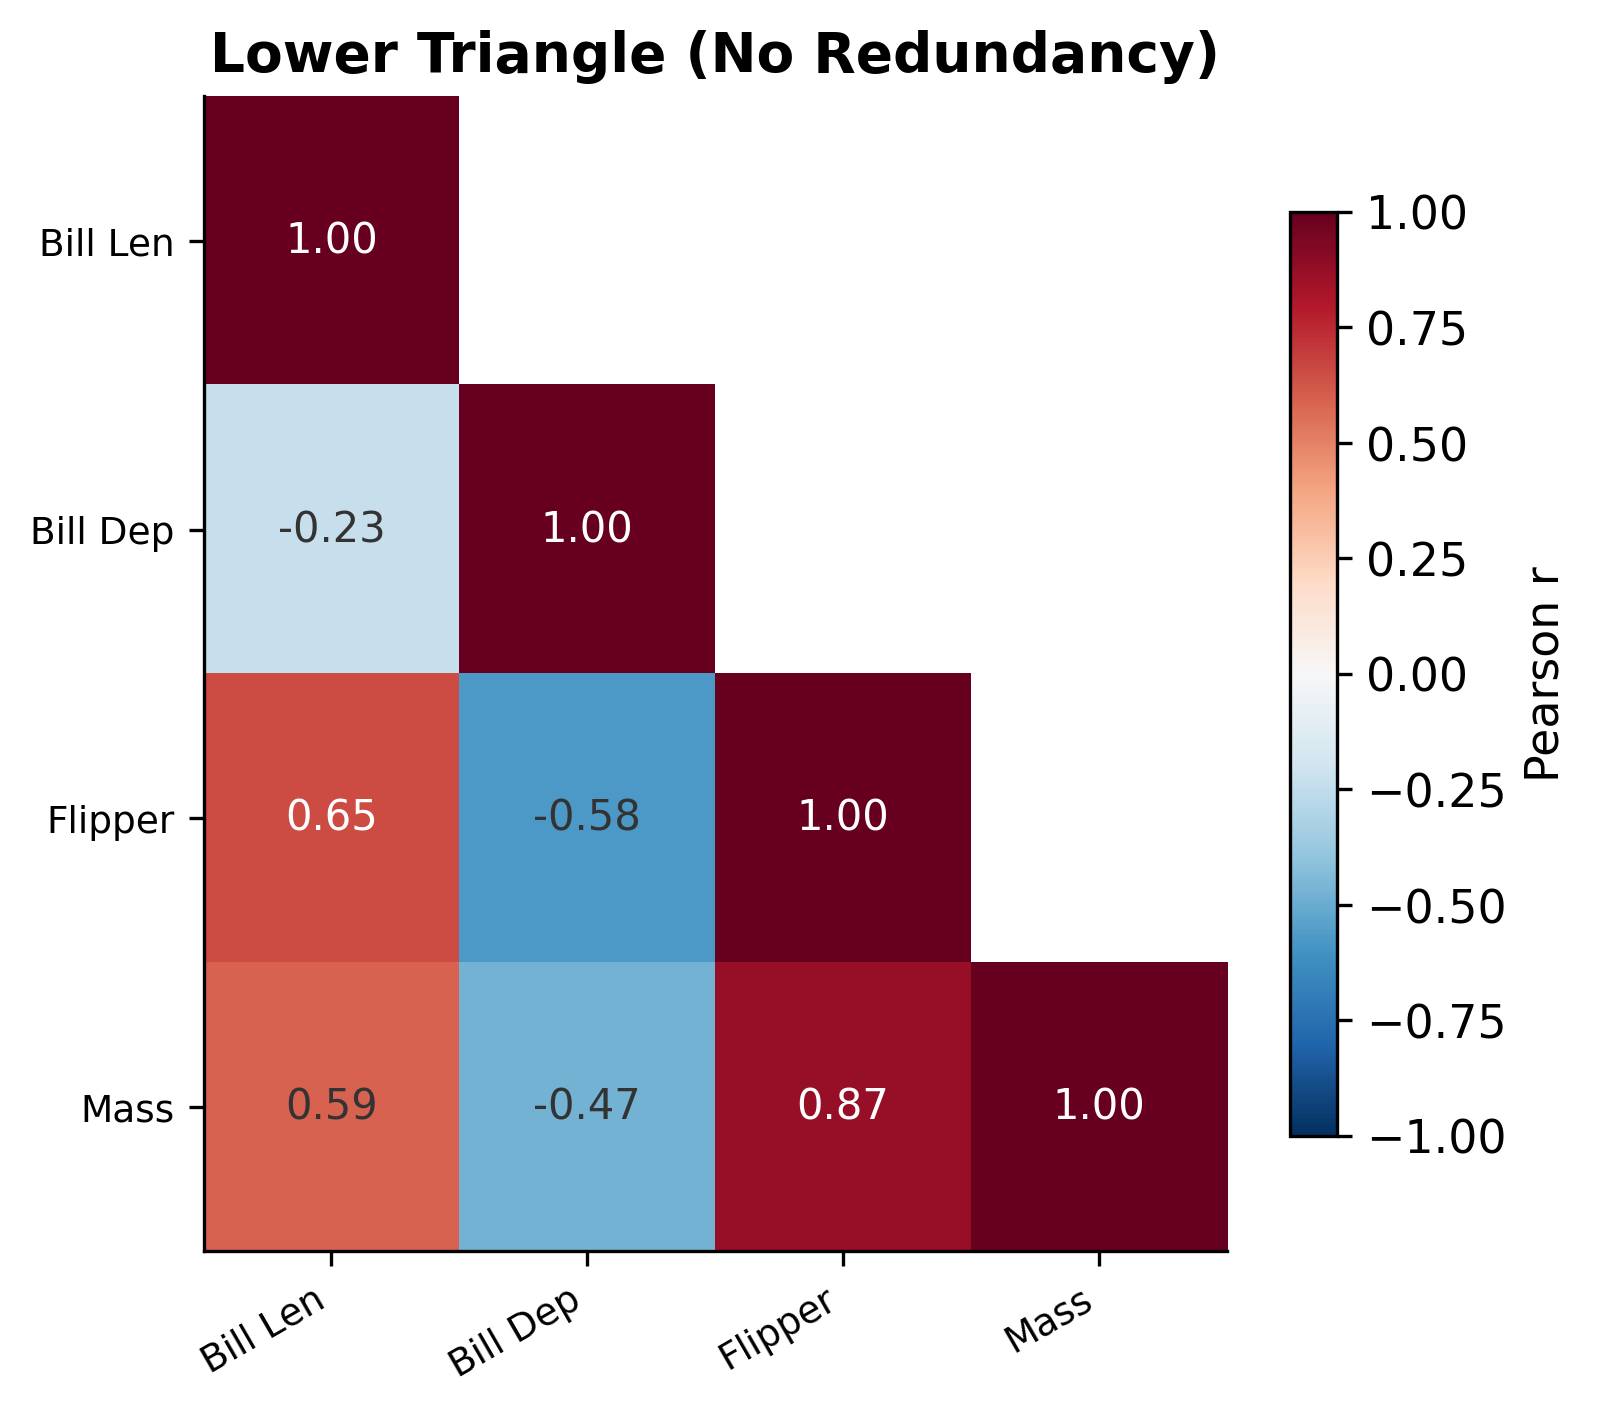
\includegraphics[width=0.55\textwidth]{m2_6_corr_lower.png}

\vspace{0.2cm}
\begin{exampleblock}{Data Insight}
    \scriptsize The correlation matrix is symmetric: $r(x, y) = r(y, x)$. Showing both halves doubles the ink for zero information gain. The lower triangle + diagonal is the convention in publications (e.g., APA style).
\end{exampleblock}
\end{frame}

% ── 158 ──
\begin{frame}[fragile]{Lower Triangle --- Code}\smark{158/300}
\begin{columns}[T]
\begin{column}{0.48\textwidth}
\begin{lstlisting}[style=Rstyle]
# ggcorrplot (dedicated package)
library(ggcorrplot)

ggcorrplot(corr,
  type = "lower",
  lab = TRUE,
  lab_size = 3.5,
  colors = c("#B2182B",
    "white", "#2166AC"),
  outline.color = "white") +
  theme_minimal()

# corrplot (base R)
library(corrplot)
corrplot(corr, type="lower",
  method="color",
  addCoef.col="#333",
  tl.col="#333")
\end{lstlisting}
\end{column}
\begin{column}{0.48\textwidth}
\begin{lstlisting}[style=Pystyle]
# seaborn with mask
mask = np.triu(
    np.ones_like(corr, dtype=bool))

fig, ax = plt.subplots(
    figsize=(6, 5))
sns.heatmap(corr,
    mask=mask,
    annot=True, fmt=".2f",
    cmap="RdBu_r",
    vmin=-1, vmax=1, center=0,
    square=True,
    linewidths=0.5,
    ax=ax)
\end{lstlisting}
\vspace{0.1cm}
\begin{exampleblock}{Data Insight}
    \scriptsize \texttt{ggcorrplot} and \texttt{corrplot} are R-specific packages optimized for correlation display. They handle masking, significance stars, and reordering out of the box.
\end{exampleblock}
\end{column}
\end{columns}
\end{frame}

% ── 159 ──
\begin{frame}{Scatterplot Matrix (Pairs Plot)}
\smark{159/300}
\centering
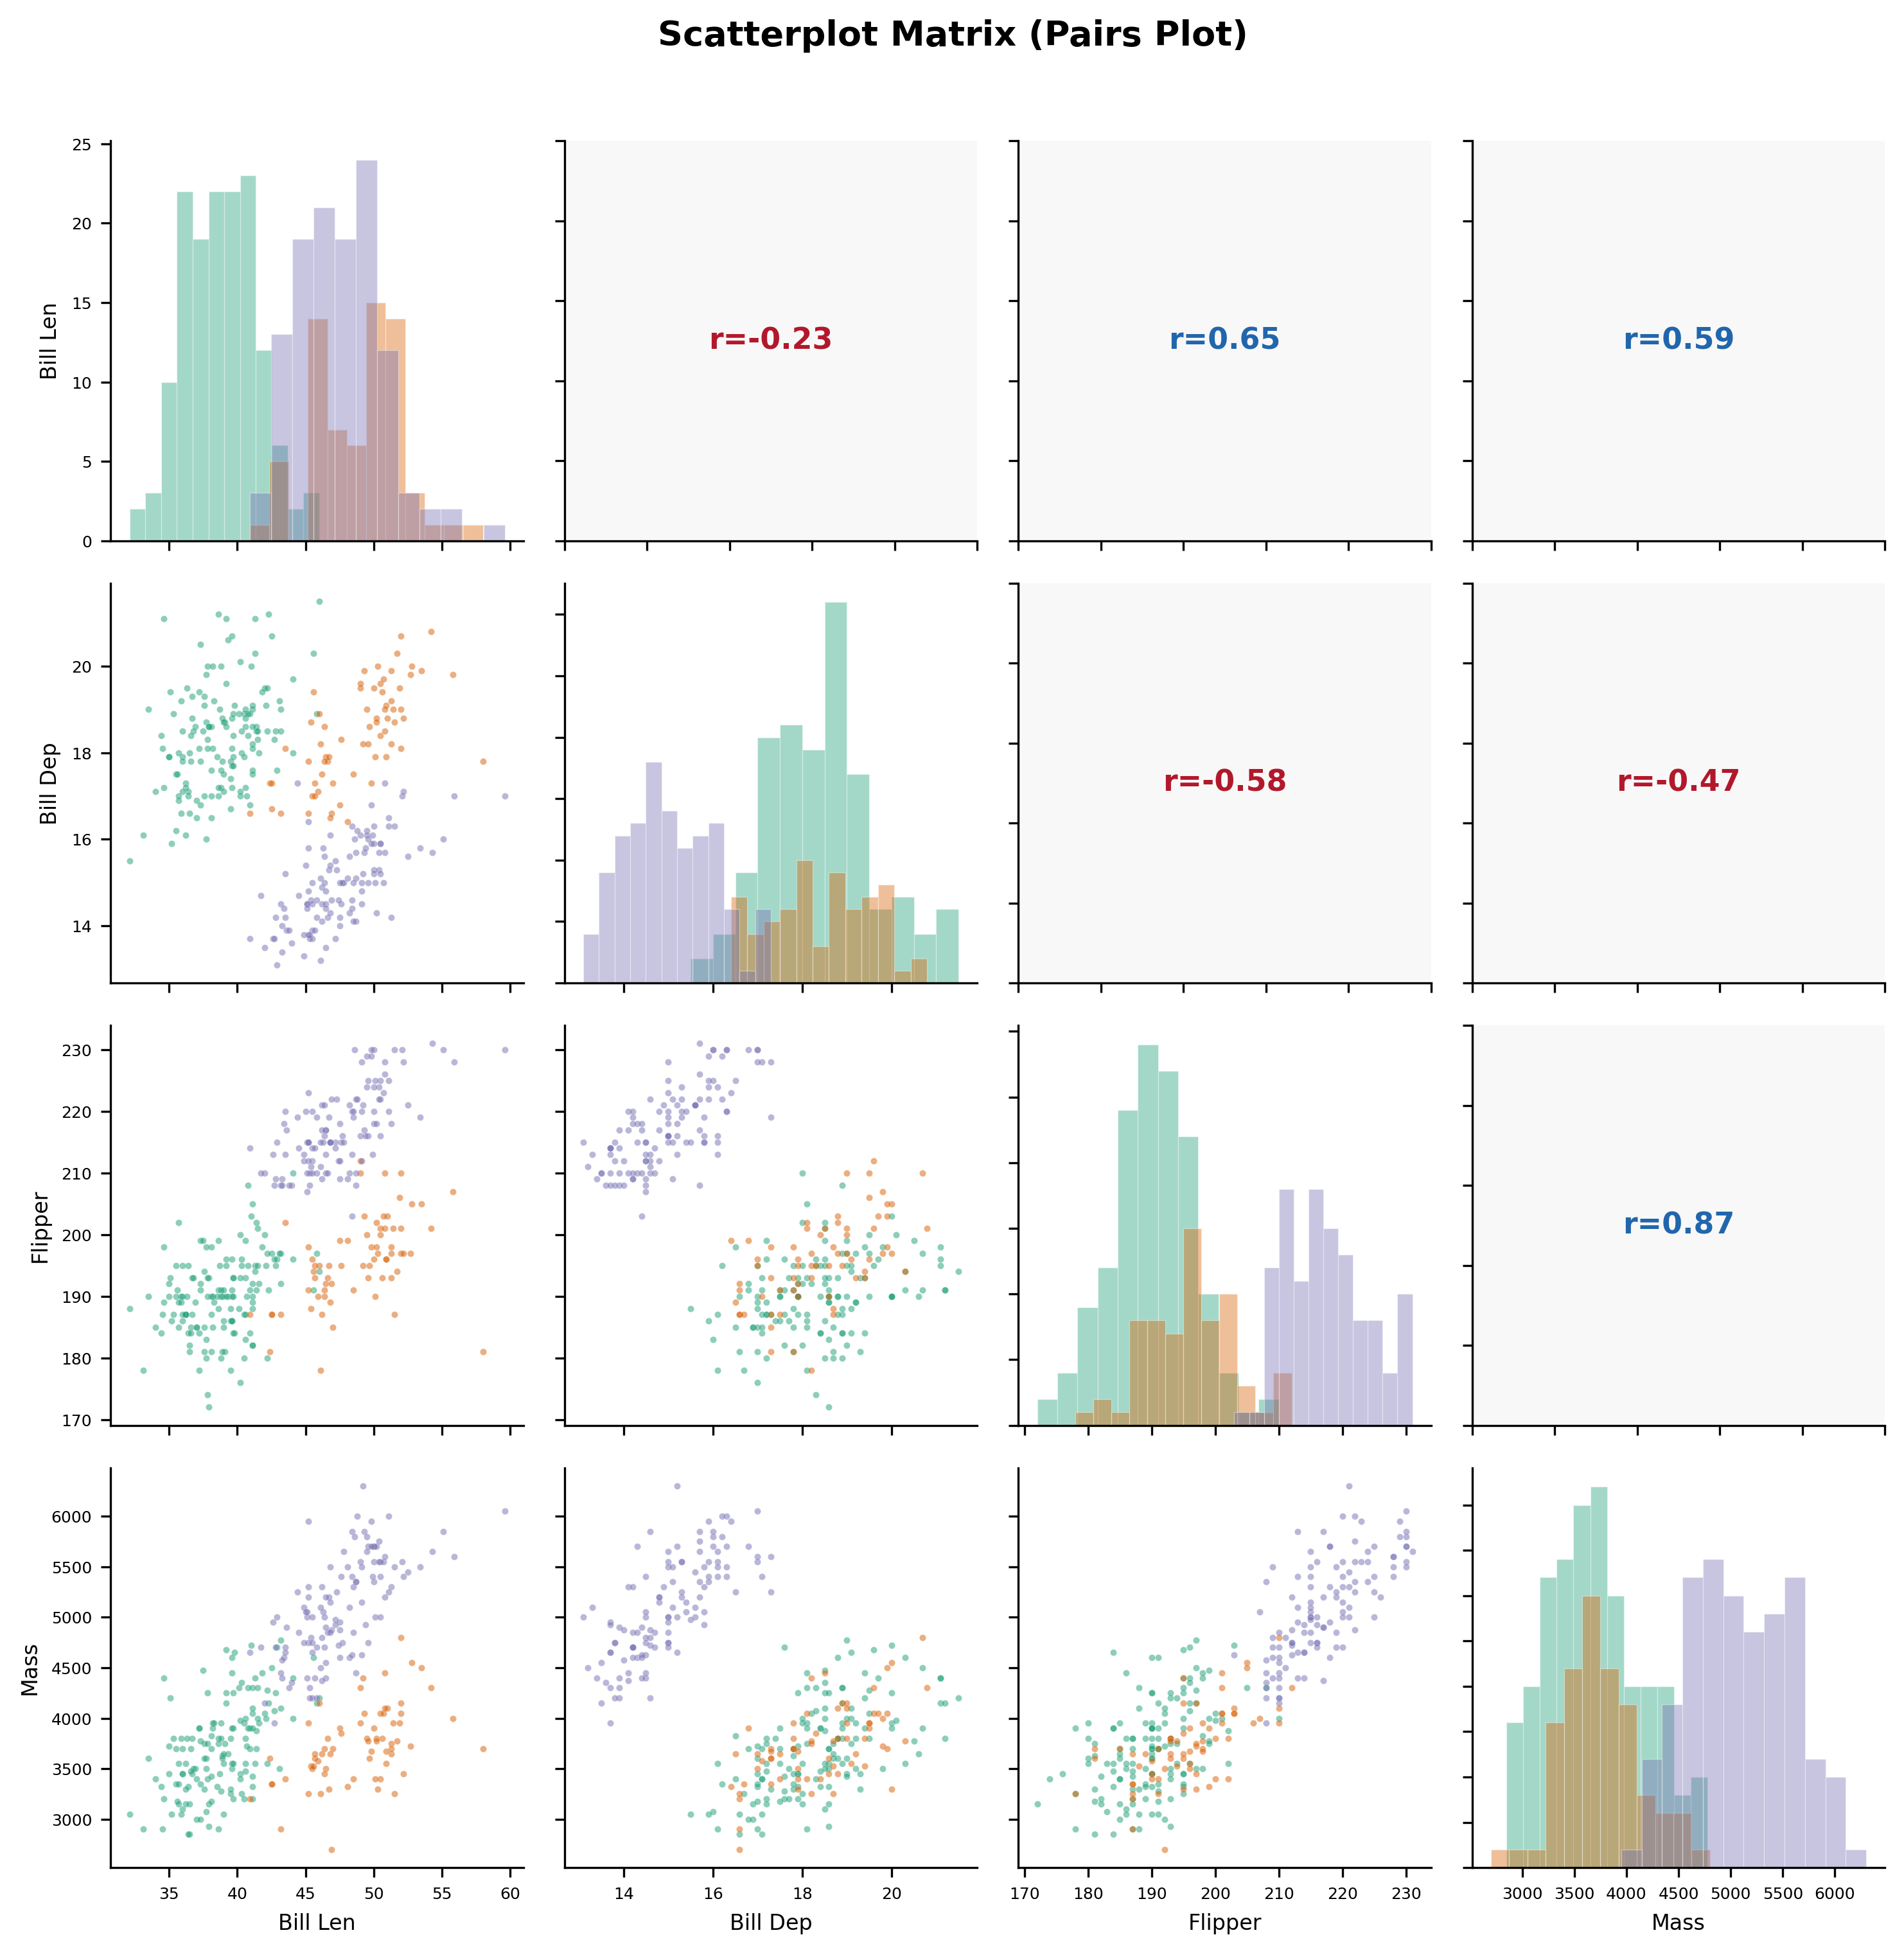
\includegraphics[width=0.65\textwidth]{m2_6_pairs.png}

\vspace{0.2cm}
\begin{exampleblock}{Data Insight}
    \scriptsize Diagonal: marginal distributions (histograms). Lower triangle: bivariate scatters colored by species. Upper triangle: numeric $r$ values. This \textbf{pairs plot} is the most comprehensive bivariate EDA display.
\end{exampleblock}
\end{frame}

% ── 160 ──
\begin{frame}[fragile]{Pairs Plot --- \Rlang}\smark{160/300}
\begin{columns}[T]
\begin{column}{0.55\textwidth}
\begin{lstlisting}[style=Rstyle]
# GGally (ggplot2-based)
library(GGally)

ggpairs(penguins,
  columns = c("bill_length_mm",
    "bill_depth_mm",
    "flipper_length_mm",
    "body_mass_g"),
  aes(color = species,
      alpha = 0.5)) +
  scale_color_manual(
    values=c("#1B9E77","#D95F02",
             "#7570B3")) +
  theme_minimal()

# Base R (quick)
pairs(penguins[, num_cols],
      col = as.integer(
        penguins$species),
      pch = 19, cex = 0.5)
\end{lstlisting}
\end{column}
\begin{column}{0.42\textwidth}
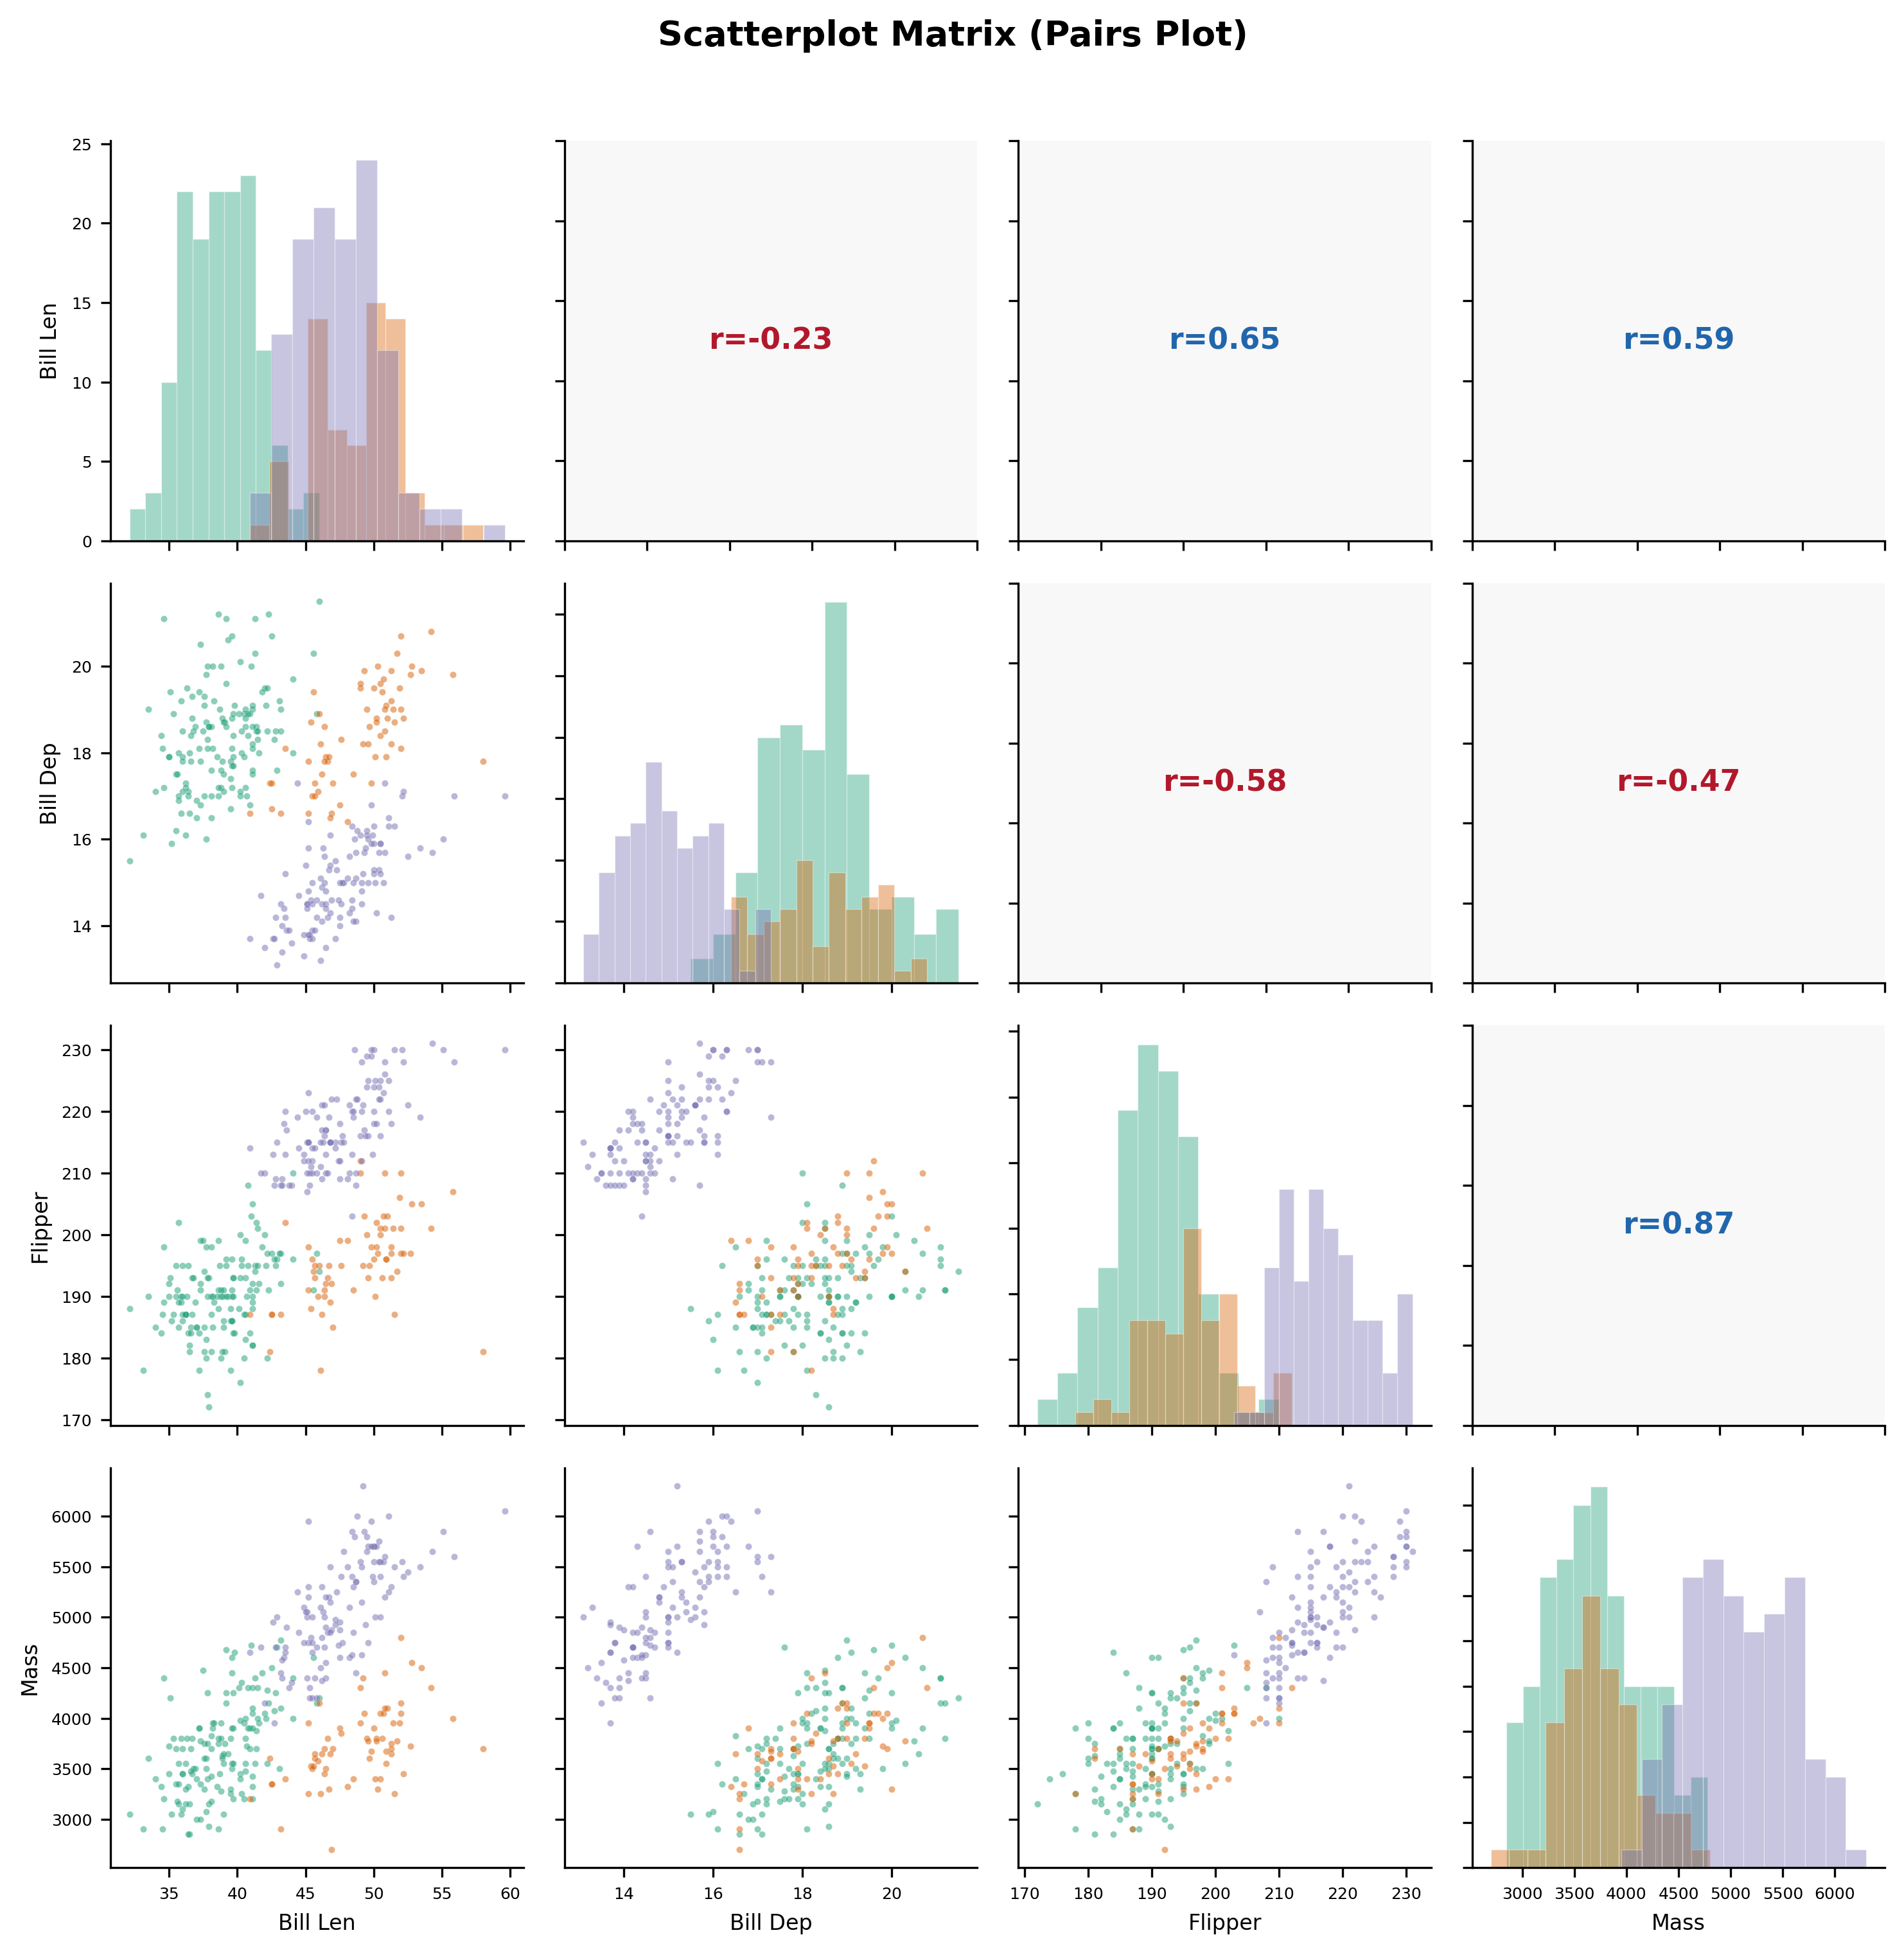
\includegraphics[width=\textwidth]{m2_6_pairs.png}
\begin{alertblock}{Pro-Tip}
    \scriptsize \texttt{GGally::ggpairs()} auto-chooses the best panel type: scatter for continuous $\times$ continuous, box/violin for continuous $\times$ categorical, bar for categorical $\times$ categorical.
\end{alertblock}
\end{column}
\end{columns}
\end{frame}

% ── 161 ──
\begin{frame}[fragile]{Pairs Plot --- \Python}\smark{161/300}
\begin{columns}[T]
\begin{column}{0.55\textwidth}
\begin{lstlisting}[style=Pystyle]
# seaborn pairplot
sns.pairplot(penguins,
    vars=["bill_length_mm",
          "bill_depth_mm",
          "flipper_length_mm",
          "body_mass_g"],
    hue="species",
    palette=["#1B9E77","#D95F02",
             "#7570B3"],
    diag_kind="hist",
    plot_kws=dict(alpha=0.5, s=10),
    height=2)

# diag_kind options:
# "hist", "kde", "auto"
# corner=True: lower triangle only
\end{lstlisting}
\end{column}
\begin{column}{0.42\textwidth}
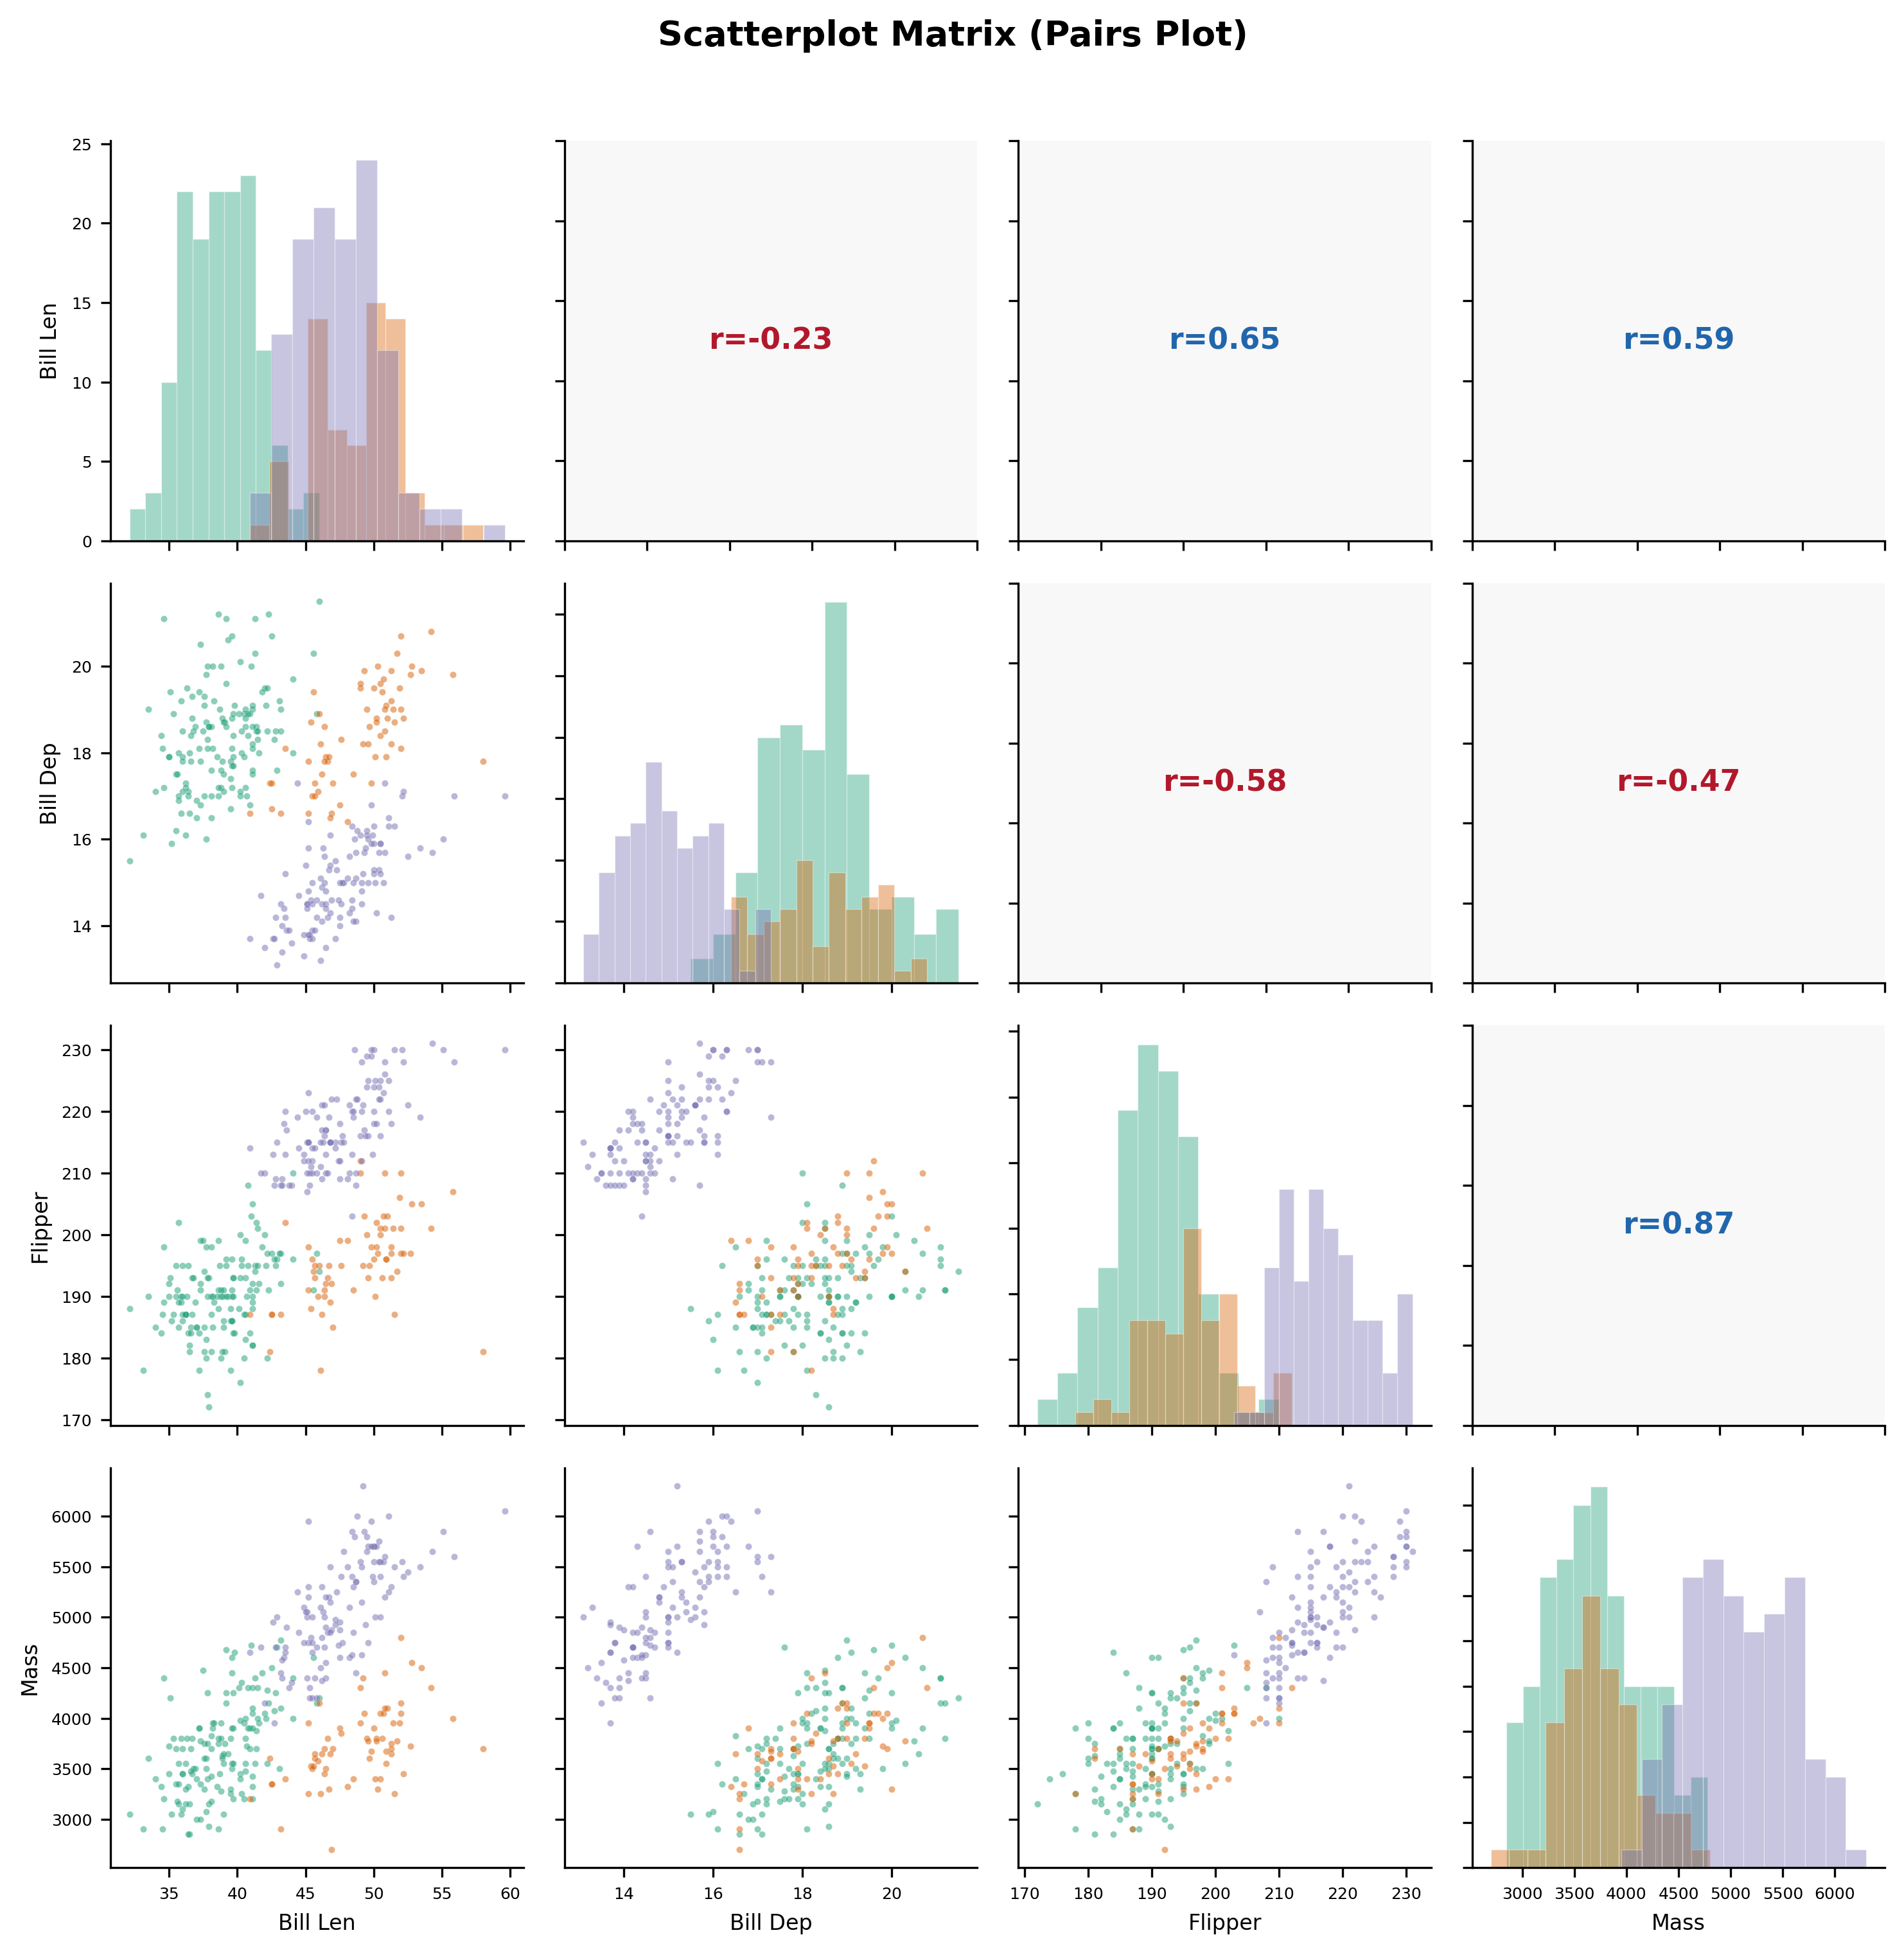
\includegraphics[width=\textwidth]{m2_6_pairs.png}
\begin{exampleblock}{Data Insight}
    \scriptsize \texttt{corner=True} produces a lower-triangle-only pairs plot, saving space and removing redundancy --- the scatterplot equivalent of the masked heatmap.
\end{exampleblock}
\end{column}
\end{columns}
\end{frame}

% ── 162 ──
\begin{frame}{Bubble Correlograms}
\smark{162/300}
\centering
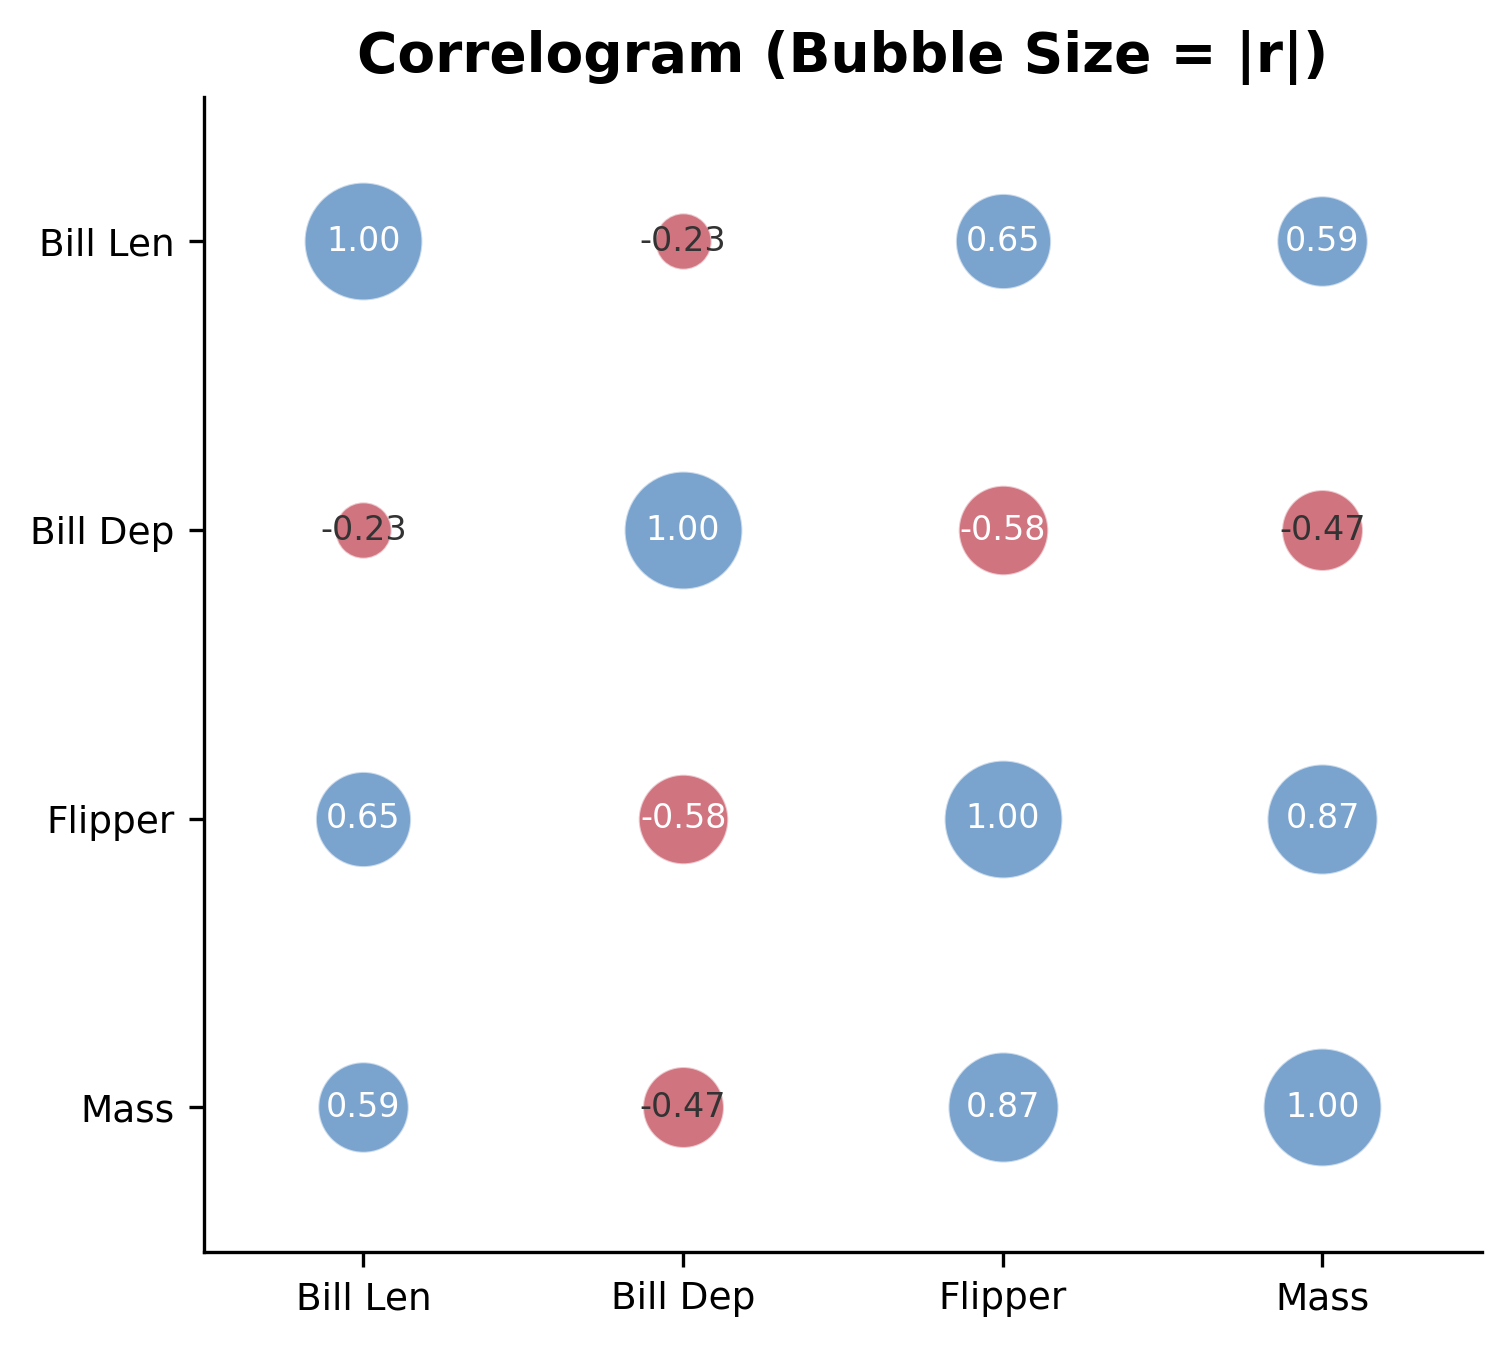
\includegraphics[width=0.55\textwidth]{m2_6_correlogram.png}

\vspace{0.2cm}
\begin{columns}[T]
\begin{column}{0.48\textwidth}
\begin{itemize}
    \item Bubble size $\propto |r|$
    \item Color = sign (blue positive, red negative)
    \item Combines magnitude and sign in one encoding
    \item More legible than heatmaps for 10+ variables
\end{itemize}
\end{column}
\begin{column}{0.48\textwidth}
\begin{alertblock}{Pro-Tip}
    \scriptsize R: \texttt{corrplot(corr, method="circle")} produces bubble correlograms. Python: manual with \texttt{ax.scatter()} and size mapped to $|r|$.
\end{alertblock}
\end{column}
\end{columns}
\end{frame}

% ── 163 ──
\begin{frame}[fragile]{Correlogram --- Code}\smark{163/300}
\begin{columns}[T]
\begin{column}{0.48\textwidth}
\begin{lstlisting}[style=Rstyle]
library(corrplot)

# Circle (bubble) correlogram
corrplot(corr,
  method = "circle",
  type = "lower",
  tl.col = "#333",
  col = colorRampPalette(
    c("#B2182B","white",
      "#2166AC"))(200))

# Ellipse variant
corrplot(corr,
  method = "ellipse",
  type = "lower",
  order = "hclust")
# hclust reorders by clustering
\end{lstlisting}
\end{column}
\begin{column}{0.48\textwidth}
\begin{lstlisting}[style=Pystyle]
# Manual bubble correlogram
fig, ax = plt.subplots()
for i in range(4):
    for j in range(4):
        r = corr.values[i, j]
        color = "#2166AC" \
            if r > 0 else "#B2182B"
        ax.scatter(j, 3-i,
            s=abs(r)*800,
            color=color, alpha=0.6)
        ax.text(j, 3-i,
            f"{r:.2f}", ha="center",
            va="center", fontsize=8)
ax.set_xticks(range(4))
ax.set_xticklabels(short_names)
\end{lstlisting}
\vspace{0.1cm}
\begin{exampleblock}{Data Insight}
    \scriptsize \texttt{order="hclust"} reorders variables by hierarchical clustering, placing correlated variables adjacent. This reveals block structure automatically.
\end{exampleblock}
\end{column}
\end{columns}
\end{frame}

% ── 164 ──
\begin{frame}{Correlation with Significance Stars}
\smark{164/300}
\centering
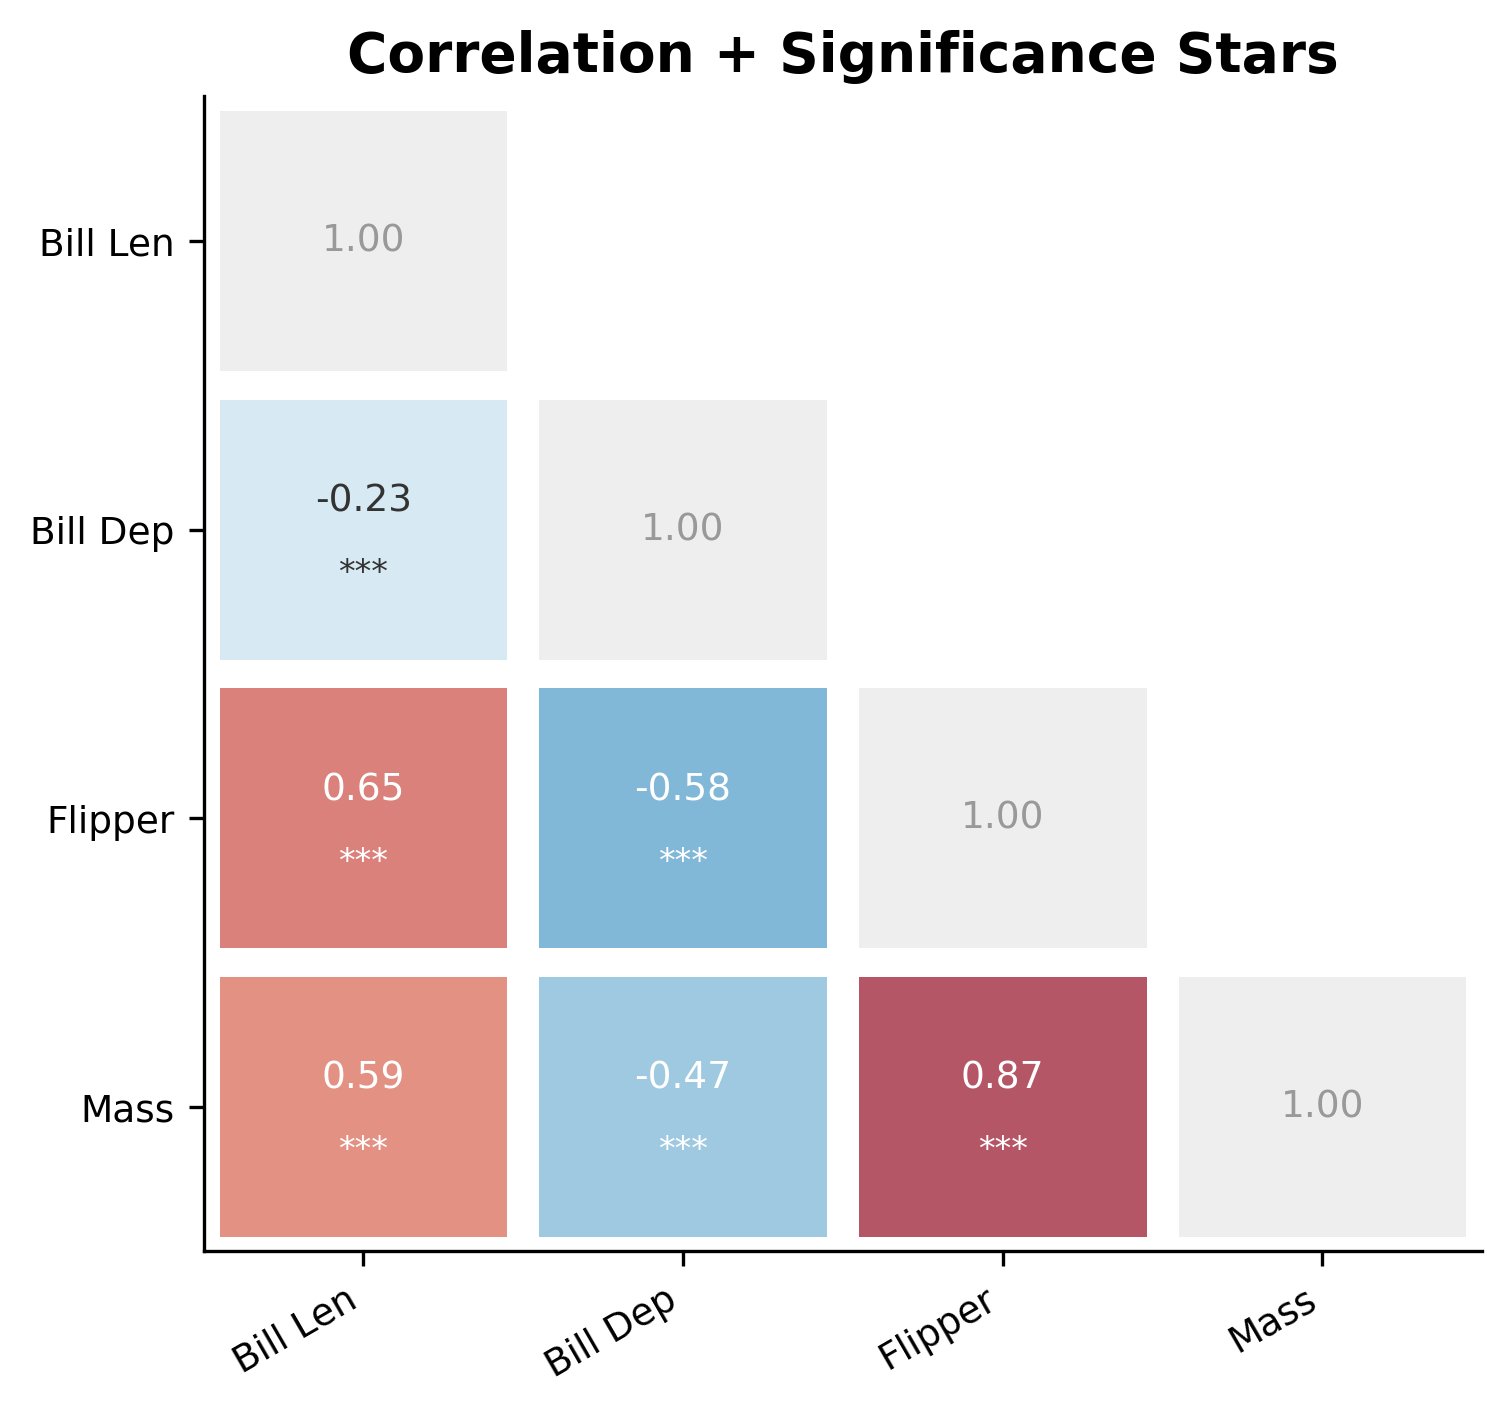
\includegraphics[width=0.55\textwidth]{m2_6_corr_stars.png}

\vspace{0.2cm}
\begin{columns}[T]
\begin{column}{0.48\textwidth}
\begin{itemize}
    \item Annotate each cell with $r$ \textbf{and} significance level
    \item Convention: * $p<0.05$, ** $p<0.01$, *** $p<0.001$
    \item Useful for exploratory screening
    \item \textbf{Not} a substitute for formal multiple-testing correction
\end{itemize}
\end{column}
\begin{column}{0.48\textwidth}
\begin{alertblock}{Pro-Tip}
    \scriptsize With $k$ variables, you test $k(k-1)/2$ pairs. At $\alpha=0.05$, expect $\sim$5\% false positives. Apply Bonferroni or FDR correction for any serious inference from correlation matrices.
\end{alertblock}
\end{column}
\end{columns}
\end{frame}

% ── 165 ──
\begin{frame}[fragile]{Significance-Annotated --- Code}\smark{165/300}
\begin{columns}[T]
\begin{column}{0.48\textwidth}
\begin{lstlisting}[style=Rstyle]
library(ggcorrplot)

# Compute p-values
p_mat <- cor_pmat(
  penguins[, num_cols])

# Heatmap with significance
ggcorrplot(corr,
  type = "lower",
  p.mat = p_mat,
  insig = "blank",  # hide ns
  lab = TRUE,
  lab_size = 3.5)

# insig options:
# "blank" = hide non-significant
# "pch"   = cross out
\end{lstlisting}
\end{column}
\begin{column}{0.48\textwidth}
\begin{lstlisting}[style=Pystyle]
from scipy.stats import pearsonr

# Compute r and p for each pair
n = len(num_cols)
p_vals = np.zeros((n, n))
for i in range(n):
    for j in range(n):
        _, p = pearsonr(
            penguins[num_cols[i]],
            penguins[num_cols[j]])
        p_vals[i, j] = p

# Annotate with stars
def stars(p):
    if p < 0.001: return "***"
    if p < 0.01: return "**"
    if p < 0.05: return "*"
    return "ns"
\end{lstlisting}
\end{column}
\end{columns}
\end{frame}

% ── 166 ──
\begin{frame}{Grouped Correlations: Faceted by Category}
\smark{166/300}
\centering
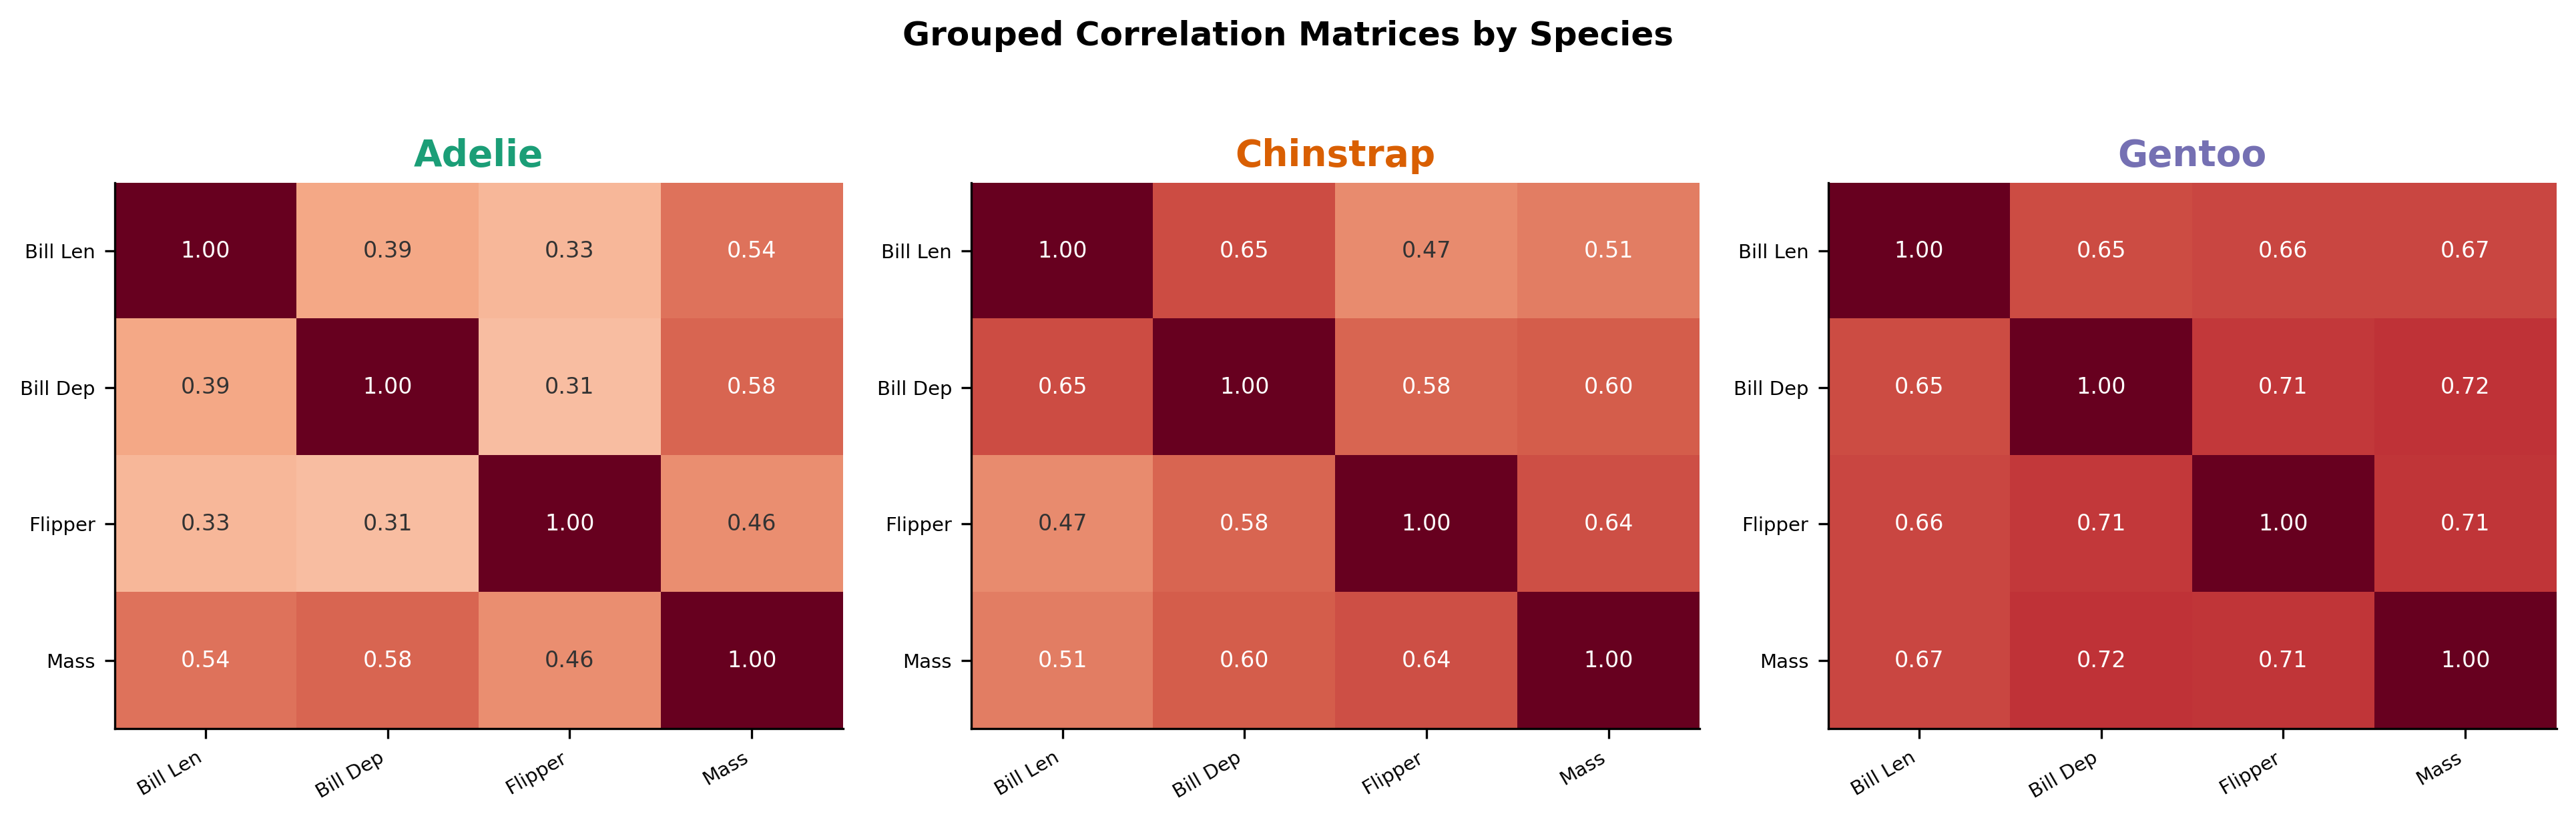
\includegraphics[width=0.88\textwidth]{m2_6_grouped_corr.png}

\vspace{0.2cm}
\begin{exampleblock}{Data Insight}
    \scriptsize Pooled: bill length and bill depth correlate at $r = -0.23$. Within Adelie: $r = +0.39$. Within Gentoo: $r = +0.64$. The grouped heatmaps make Simpson's paradox visible across \emph{all} variable pairs simultaneously.
\end{exampleblock}
\end{frame}

% ── 167 ──
\begin{frame}[fragile]{Grouped Correlations --- Code}\smark{167/300}
\begin{columns}[T]
\begin{column}{0.48\textwidth}
\begin{lstlisting}[style=Rstyle]
library(purrr)
library(ggcorrplot)

# One heatmap per species
penguins |>
  group_split(species) |>
  map(function(df) {
    corr <- cor(df[, num_cols],
      use="complete.obs")
    ggcorrplot(corr,
      type="lower", lab=TRUE,
      title=unique(df$species))
  })

# Or patchwork for side-by-side
library(patchwork)
p1 | p2 | p3
\end{lstlisting}
\end{column}
\begin{column}{0.48\textwidth}
\begin{lstlisting}[style=Pystyle]
fig, axes = plt.subplots(1, 3,
    figsize=(14, 4))

for ax, sp in zip(axes,
    species_list):
    sub = penguins[
        penguins["species"]==sp]
    sub_corr = sub[num_cols].corr()
    sns.heatmap(sub_corr,
        annot=True, fmt=".2f",
        cmap="RdBu_r",
        vmin=-1, vmax=1,
        center=0, ax=ax,
        cbar=False)
    ax.set_title(sp,
        fontweight="bold")
\end{lstlisting}
\vspace{0.1cm}
\begin{alertblock}{Pro-Tip}
    \scriptsize Comparing grouped heatmaps requires \textbf{identical color scales}. Always set \texttt{vmin=-1, vmax=1} explicitly to prevent per-panel rescaling.
\end{alertblock}
\end{column}
\end{columns}
\end{frame}

% ── 168 ──
\begin{frame}{Aggregated Heatmaps: Cross-Tabulated Values}
\smark{168/300}
\centering
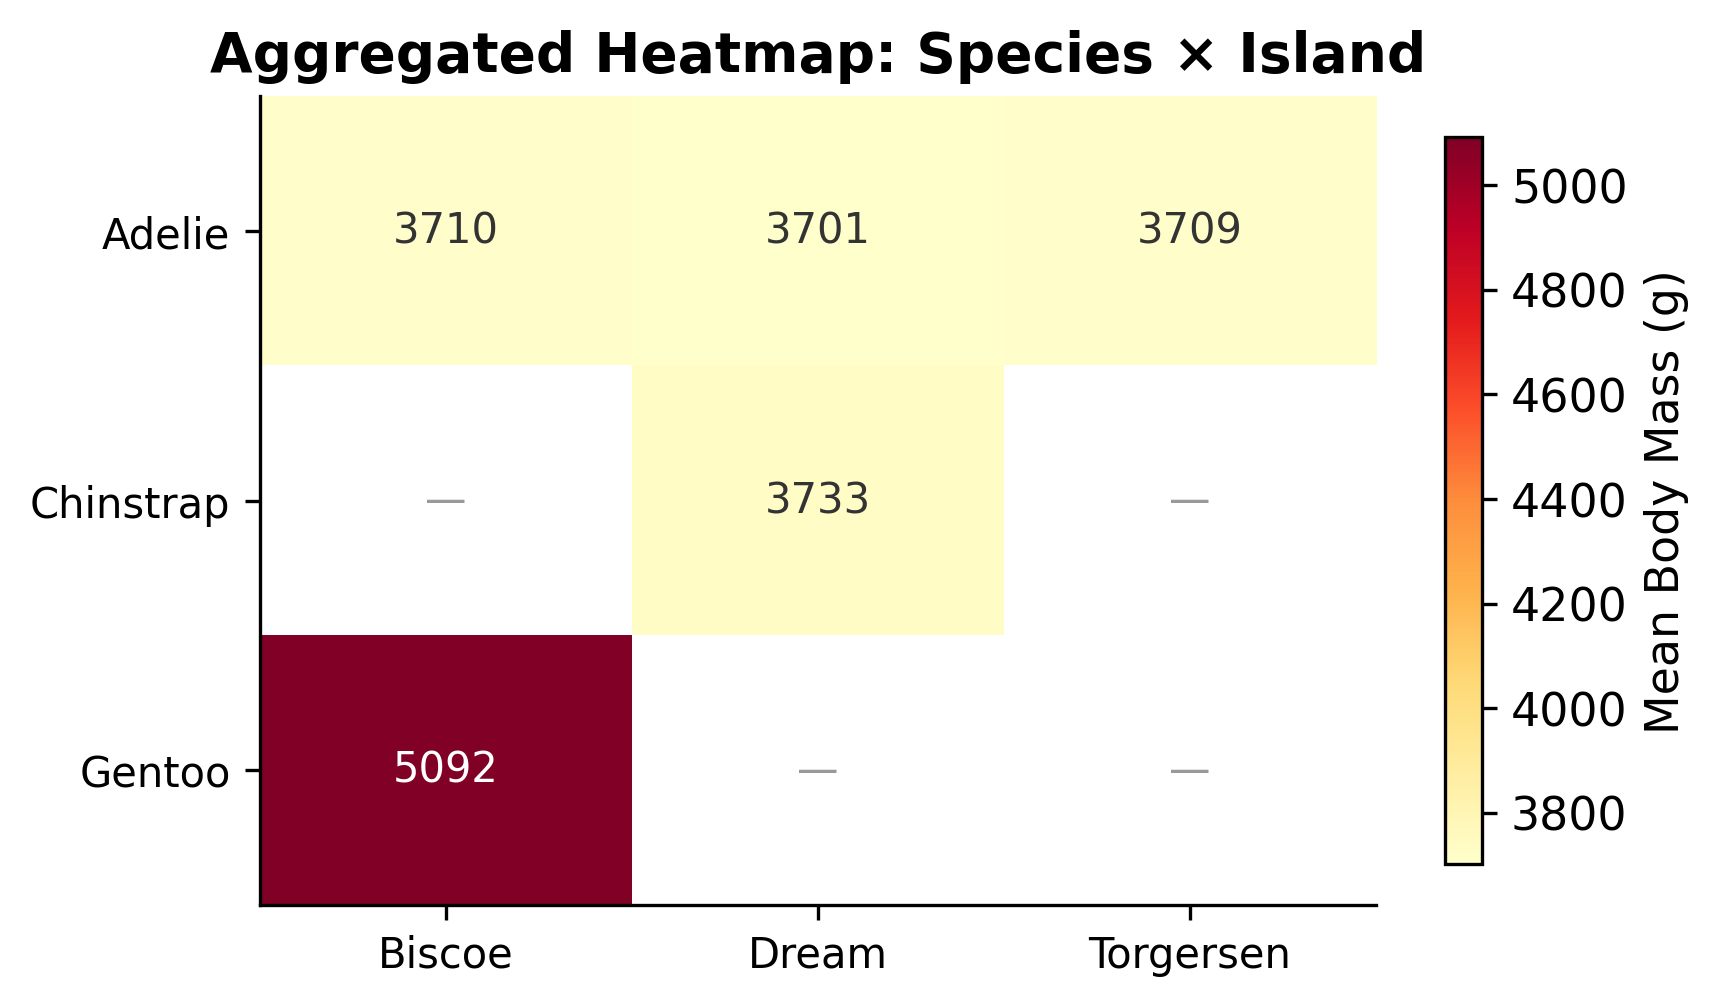
\includegraphics[width=0.62\textwidth]{m2_6_agg_heatmap.png}

\vspace{0.2cm}
\begin{columns}[T]
\begin{column}{0.48\textwidth}
\begin{itemize}
    \item Not correlations --- \textbf{any} aggregated value (mean, count, proportion)
    \item Rows and columns = categorical variables
    \item Cells = summary statistic
    \item Missing cells (``---'') are informative: Chinstrap are absent from Biscoe and Torgersen
\end{itemize}
\end{column}
\begin{column}{0.48\textwidth}
\begin{exampleblock}{Data Insight}
    \scriptsize Heatmaps of means are more informative than grouped bar charts when you have a full row $\times$ column layout. The color gradient reveals patterns that bars cannot (e.g., a diagonal trend).
\end{exampleblock}
\end{column}
\end{columns}
\end{frame}

% ── 169 ──
\begin{frame}[fragile]{Aggregated Heatmap --- Code}\smark{169/300}
\begin{columns}[T]
\begin{column}{0.48\textwidth}
\begin{lstlisting}[style=Rstyle]
pivot <- penguins |>
  group_by(species, island) |>
  summarise(mean_mass =
    mean(body_mass_g)) |>
  pivot_wider(names_from=island,
    values_from=mean_mass)

# geom_tile
ggplot(long_df,
  aes(island, species,
      fill=mean_mass)) +
  geom_tile(color="white") +
  geom_text(aes(
    label=round(mean_mass)),
    size=3.5) +
  scale_fill_viridis_c() +
  theme_minimal()
\end{lstlisting}
\end{column}
\begin{column}{0.48\textwidth}
\begin{lstlisting}[style=Pystyle]
pivot = penguins.pivot_table(
    values="body_mass_g",
    index="species",
    columns="island",
    aggfunc="mean")

sns.heatmap(pivot,
    annot=True, fmt=".0f",
    cmap="YlOrRd",
    linewidths=0.5)

# geom_tile in plotnine
(ggplot(long_df,
   aes("island","species",
       fill="mean_mass"))
 + geom_tile(color="white")
 + geom_text(aes(label="label"))
 + scale_fill_cmap("viridis"))
\end{lstlisting}
\end{column}
\end{columns}
\end{frame}

% ── 170 ──
\begin{frame}{Reordering Variables: Hierarchical Clustering}
\smark{170/300}
\begin{columns}[T]
\begin{column}{0.50\textwidth}
\begin{itemize}
    \item Default order: alphabetical or input order
    \item \textbf{Hierarchical clustering} groups correlated variables adjacent
    \item Reveals \textbf{block structure}: clusters of co-varying features
    \item Essential for 10+ variables --- alphabetical order hides patterns
\end{itemize}
\end{column}
\begin{column}{0.47\textwidth}
\begin{alertblock}{Pro-Tip}
    \scriptsize R: \texttt{corrplot(corr, order="hclust")} or \texttt{ggcorrplot(corr, hc.order=TRUE)}. Python: \texttt{sns.clustermap(corr)} which adds dendrograms automatically.
\end{alertblock}
\vspace{0.2cm}
\begin{exampleblock}{Data Insight}
    \scriptsize \texttt{sns.clustermap()} is a combined heatmap + dendrogram. It clusters both rows and columns simultaneously, revealing hierarchical structure in the variable space.
\end{exampleblock}
\end{column}
\end{columns}
\end{frame}

% ── 171 ──
\begin{frame}[fragile]{Clustered Heatmap --- Code}\smark{171/300}
\begin{columns}[T]
\begin{column}{0.48\textwidth}
\begin{lstlisting}[style=Rstyle]
# corrplot with clustering
corrplot(corr,
  order = "hclust",
  addrect = 2, # draw 2 clusters
  method = "color",
  type = "lower",
  addCoef.col = "#333")

# ggcorrplot
ggcorrplot(corr,
  hc.order = TRUE,
  type = "lower",
  lab = TRUE)
\end{lstlisting}
\end{column}
\begin{column}{0.48\textwidth}
\begin{lstlisting}[style=Pystyle]
# seaborn clustermap
g = sns.clustermap(corr,
    annot=True, fmt=".2f",
    cmap="RdBu_r",
    vmin=-1, vmax=1, center=0,
    linewidths=0.5,
    figsize=(6, 6),
    dendrogram_ratio=0.15)

# method: ward, complete, average
g = sns.clustermap(corr,
    method="ward",
    metric="euclidean")
\end{lstlisting}
\end{column}
\end{columns}
\end{frame}

% ── 172 ──
\begin{frame}{Large Correlation Matrices: Strategies}
\smark{172/300}
\begin{columns}[T]
\begin{column}{0.50\textwidth}
    \textbf{$p < 20$ variables:}
    \begin{itemize}
        \item Full heatmap with annotations
        \item Clustered reordering
        \item Pairs plot (if $p \leq 8$)
    \end{itemize}
    \vspace{0.2cm}
    \textbf{$20 < p < 100$:}
    \begin{itemize}
        \item Clustermap without annotations
        \item Bubble correlogram (size = $|r|$)
        \item Focus on one row/column at a time
    \end{itemize}
\end{column}
\begin{column}{0.47\textwidth}
    \textbf{$p > 100$ (genomics, NLP):}
    \begin{itemize}
        \item Heatmaps of PCA-reduced subset
        \item Network graph (Workshop 7): nodes = variables, edges = high $|r|$
        \item Interactive: zoom/filter in plotly or ComplexHeatmap
    \end{itemize}
    \vspace{0.1cm}
    \begin{alertblock}{Pro-Tip}
        \scriptsize For $p > 100$, \texttt{ComplexHeatmap} (R/Bioconductor) is the gold standard. Python: \texttt{seaborn.clustermap()} scales well to $\sim$200.
    \end{alertblock}
\end{column}
\end{columns}
\end{frame}

% ── 173 ──
\begin{frame}{Correlation $\neq$ Causation: Visual Reminders}
\smark{173/300}
\begin{columns}[T]
\begin{column}{0.50\textwidth}
\begin{itemize}
    \item $r = 0.95$ between ice cream sales and drownings does not mean ice cream causes drowning
    \item Confounders (temperature), reverse causation, and coincidence all produce high $r$
    \item Correlation $\to$ ``these variables move together'' $\to$ \textbf{investigate further}
    \item Causal claims require experiments or causal inference frameworks (DAGs)
\end{itemize}
\end{column}
\begin{column}{0.47\textwidth}
\begin{exampleblock}{Data Insight}
    \scriptsize Vigen's \textit{Spurious Correlations} website shows $r > 0.9$ between, e.g., US cheese consumption and deaths by bedsheet entanglement. The visual is humorous but makes a serious point about confounding.
\end{exampleblock}
\vspace{0.1cm}
\begin{alertblock}{Pro-Tip}
    \scriptsize Label correlation displays as ``\textbf{Association}'' not ``\textbf{Effect}.'' Captions matter: ``Bill length is associated with body mass'' not ``Bill length determines body mass.''
\end{alertblock}
\end{column}
\end{columns}
\end{frame}

% ── 174 ──
\begin{frame}{Partial Correlation: Controlling for Confounds}
\smark{174/300}
\begin{columns}[T]
\begin{column}{0.50\textwidth}
\begin{itemize}
    \item Partial $r$: correlation between $x$ and $y$ \textbf{after removing} the linear effect of $z$
    \item If $r_{xy} = 0.8$ but $r_{xy \cdot z} = 0.1$, the association was driven by $z$
    \item Visualize with added-variable plots (Module 2.3) or partial correlation heatmaps
\end{itemize}
\end{column}
\begin{column}{0.47\textwidth}
\begin{alertblock}{Pro-Tip}
    \scriptsize R: \texttt{ppcor::pcor()} computes the full partial correlation matrix. Python: \texttt{pingouin.partial\_corr()} for pairwise, or compute from the inverse correlation matrix ($\Sigma^{-1}$).
\end{alertblock}
\vspace{0.1cm}
\begin{exampleblock}{Data Insight}
    \scriptsize The partial correlation matrix is what a multiple regression ``sees.'' It is the true pairwise structure after removing mutual confounds --- often very different from the raw Pearson matrix.
\end{exampleblock}
\end{column}
\end{columns}
\end{frame}

% ── 175 ──
\begin{frame}[fragile]{Partial Correlation --- Code}\smark{175/300}
\begin{columns}[T]
\begin{column}{0.48\textwidth}
\begin{lstlisting}[style=Rstyle]
library(ppcor)

# Full partial correlation matrix
pc <- pcor(penguins[, num_cols],
           method = "pearson")
pc$estimate  # partial r
pc$p.value   # p-values

# Visualize
ggcorrplot(pc$estimate,
  type = "lower", lab = TRUE,
  title = "Partial Correlations")

# Single pair, controlling for z
pcor.test(x, y, z,
          method = "pearson")
\end{lstlisting}
\end{column}
\begin{column}{0.48\textwidth}
\begin{lstlisting}[style=Pystyle]
import pingouin as pg

# Pairwise partial correlation
pc = pg.partial_corr(
    data=penguins,
    x="bill_length_mm",
    y="body_mass_g",
    covar="flipper_length_mm")

# Full matrix via inverse
from numpy.linalg import inv
corr_mat = penguins[num_cols]\
    .corr().values
P = inv(corr_mat)
# Partial r: -P[i,j] / sqrt(P[i,i]*P[j,j])
\end{lstlisting}
\vspace{0.1cm}
\begin{exampleblock}{Data Insight}
    \scriptsize \texttt{pingouin} is the cleanest Python interface for correlation analysis. It provides Pearson, Spearman, partial, and semi-partial correlations with Bayesian factors.
\end{exampleblock}
\end{column}
\end{columns}
\end{frame}

% ── 176 ──
\begin{frame}{Heatmap Design Principles}
\smark{176/300}
\centering\small
\begin{tabular}{@{}ll@{}}
    \toprule
    \textbf{Principle} & \textbf{Implementation} \\
    \midrule
    Diverging palette for signed data    & \texttt{RdBu\_r}, centered at 0 \\
    Sequential palette for unsigned data & \texttt{viridis}, \texttt{YlOrRd} \\
    Annotate cells with numbers          & \texttt{annot=True} or \texttt{geom\_text()} \\
    Remove redundancy                    & Mask upper triangle \\
    Reorder by clustering                & \texttt{order="hclust"} / \texttt{clustermap()} \\
    White cell borders                   & \texttt{linewidths=0.5} \\
    Fixed color scale                    & \texttt{vmin=-1, vmax=1} for correlations \\
    Square aspect ratio                  & \texttt{square=True} or \texttt{coord\_fixed()} \\
    \bottomrule
\end{tabular}

\vspace{0.3cm}
\begin{alertblock}{Pro-Tip}
    \scriptsize The single most impactful heatmap improvement: \textbf{cluster-reorder} the variables. It transforms a noisy grid into a block-diagonal structure that reveals the data's natural grouping.
\end{alertblock}
\end{frame}

% ── 177 ──
\begin{frame}{Alternatives to Heatmaps}
\smark{177/300}
\begin{columns}[T]
\begin{column}{0.50\textwidth}
    \textbf{When heatmaps fail:}
    \begin{itemize}
        \item Exact values hard to read from color alone
        \item Color discrimination limited to $\sim$5--7 levels
        \item Small differences invisible
        \item Colorblind-unfriendly with many palettes
    \end{itemize}
\end{column}
\begin{column}{0.47\textwidth}
    \textbf{Alternatives:}
    \begin{itemize}
        \item \textbf{Dot matrix}: size + color (correlogram)
        \item \textbf{Parallel coordinates}: Module 5
        \item \textbf{Network graph}: edges = high $|r|$ (Module 7)
        \item \textbf{Trellis/faceted scatter}: one panel per pair
        \item \textbf{Table with conditional formatting}: for exact values
    \end{itemize}
\end{column}
\end{columns}
\end{frame}

% ── 178 ──
\begin{frame}{Correlation for Non-Numeric Data}
\smark{178/300}
\centering\small
\begin{tabular}{@{}llll@{}}
    \toprule
    \textbf{Variable Types} & \textbf{Association} & \textbf{R} & \textbf{Python} \\
    \midrule
    Continuous $\times$ Continuous & Pearson/Spearman $r$ & \texttt{cor()} & \texttt{.corr()} \\
    Ordinal $\times$ Ordinal       & Spearman $\rho$ / Kendall $\tau$ & \texttt{cor(method="spearman")} & \texttt{.corr(method="spearman")} \\
    Categorical $\times$ Categorical & Cramér's $V$ / $\chi^2$ & \texttt{vcd::assocstats()} & \texttt{scipy.stats.chi2\_contingency()} \\
    Continuous $\times$ Categorical  & Point-biserial $r$ / $\eta^2$ & \texttt{ltm::biserial.cor()} & \texttt{pg.compute\_effsize()} \\
    \bottomrule
\end{tabular}

\vspace{0.3cm}
\begin{exampleblock}{Data Insight}
    \scriptsize Workshop 3 (Categorical Data) covers Cramér's $V$, mosaic plots, and association plots in full. Module 2.6 focuses on continuous-variable correlation and heatmap design.
\end{exampleblock}
\end{frame}

% ── 179 ──
\begin{frame}{Correlation Decision Guide}
\smark{179/300}
\centering\small
\begin{tabular}{@{}lll@{}}
    \toprule
    \textbf{Task} & \textbf{Plot} & \textbf{Tool} \\
    \midrule
    Quick overview ($p < 10$)     & Heatmap (lower triangle) & \texttt{ggcorrplot} / \texttt{sns.heatmap} \\
    Bivariate detail ($p \leq 8$) & Pairs plot               & \texttt{GGally::ggpairs} / \texttt{sns.pairplot} \\
    Many variables ($10 < p < 50$)& Clustered heatmap        & \texttt{corrplot} / \texttt{sns.clustermap} \\
    Bubble encoding               & Correlogram              & \texttt{corrplot(method="circle")} \\
    Controlling confounds          & Partial correlation      & \texttt{ppcor::pcor} / \texttt{pingouin} \\
    Aggregated summaries           & \texttt{geom\_tile()}    & \texttt{pivot\_table} + heatmap \\
    Grouped by category            & Faceted heatmaps         & \texttt{group\_split} / loop \\
    \bottomrule
\end{tabular}
\end{frame}

% ── 180 ──
\begin{frame}{Module 2.6 --- Key Takeaways}\smark{180/300}
\begin{enumerate}
    \item \textbf{Diverging palette centered at zero} for correlation heatmaps. Always.
    \item \textbf{Mask the upper triangle} --- it's redundant.
    \item \textbf{Cluster-reorder} variables to reveal block structure.
    \item \textbf{Pairs plots} for bivariate detail; heatmaps for overview.
    \item \textbf{Grouped correlations} expose Simpson's paradox across all pairs.
    \item \textbf{Partial correlations} remove confounds --- often very different from raw $r$.
\end{enumerate}
\end{frame}

% ── 181 ──
\begin{frame}{}\smark{181/300}
\centering\vspace{1.5cm}
{\Large\textbf{Module 2.6 Complete}}\\[0.5cm]
You can now visualize pairwise associations with heatmaps, pairs plots, correlograms, and clustered displays --- with proper masking, annotation, significance, and confound control.\\[0.5cm]
\textbf{Next:} Module 2.7 --- Hypothesis Test Visualization and $p$-Value Displays.
\end{frame}

% ═══════════════════════════════════════════════════════
%  MODULE 2.7 — Hypothesis Test Visualization and p-Value Displays
% ═══════════════════════════════════════════════════════
\section{Module 2.7 --- Hypothesis Tests and $p$-Value Displays}

% ── 182 ──
\begin{frame}{Module 2.7 --- Roadmap}\smark{182/300}
\begin{enumerate}
    \item Visualizing the null distribution and observed test statistic
    \item $p$-value as tail area: geometric intuition
    \item Effect size visualization (Cohen's $d$ overlap)
    \item Estimation plots: the Gardner--Altman and Cumming designs
    \item Significance brackets: when (rarely) to use them
    \item Volcano plots for high-dimensional testing
    \item Power curves and sample-size planning
    \item The new statistics: estimation over $p$-values
\end{enumerate}
\end{frame}

% ── 183 ──
\begin{frame}{Visualizing the Null Distribution}
\smark{183/300}
\centering
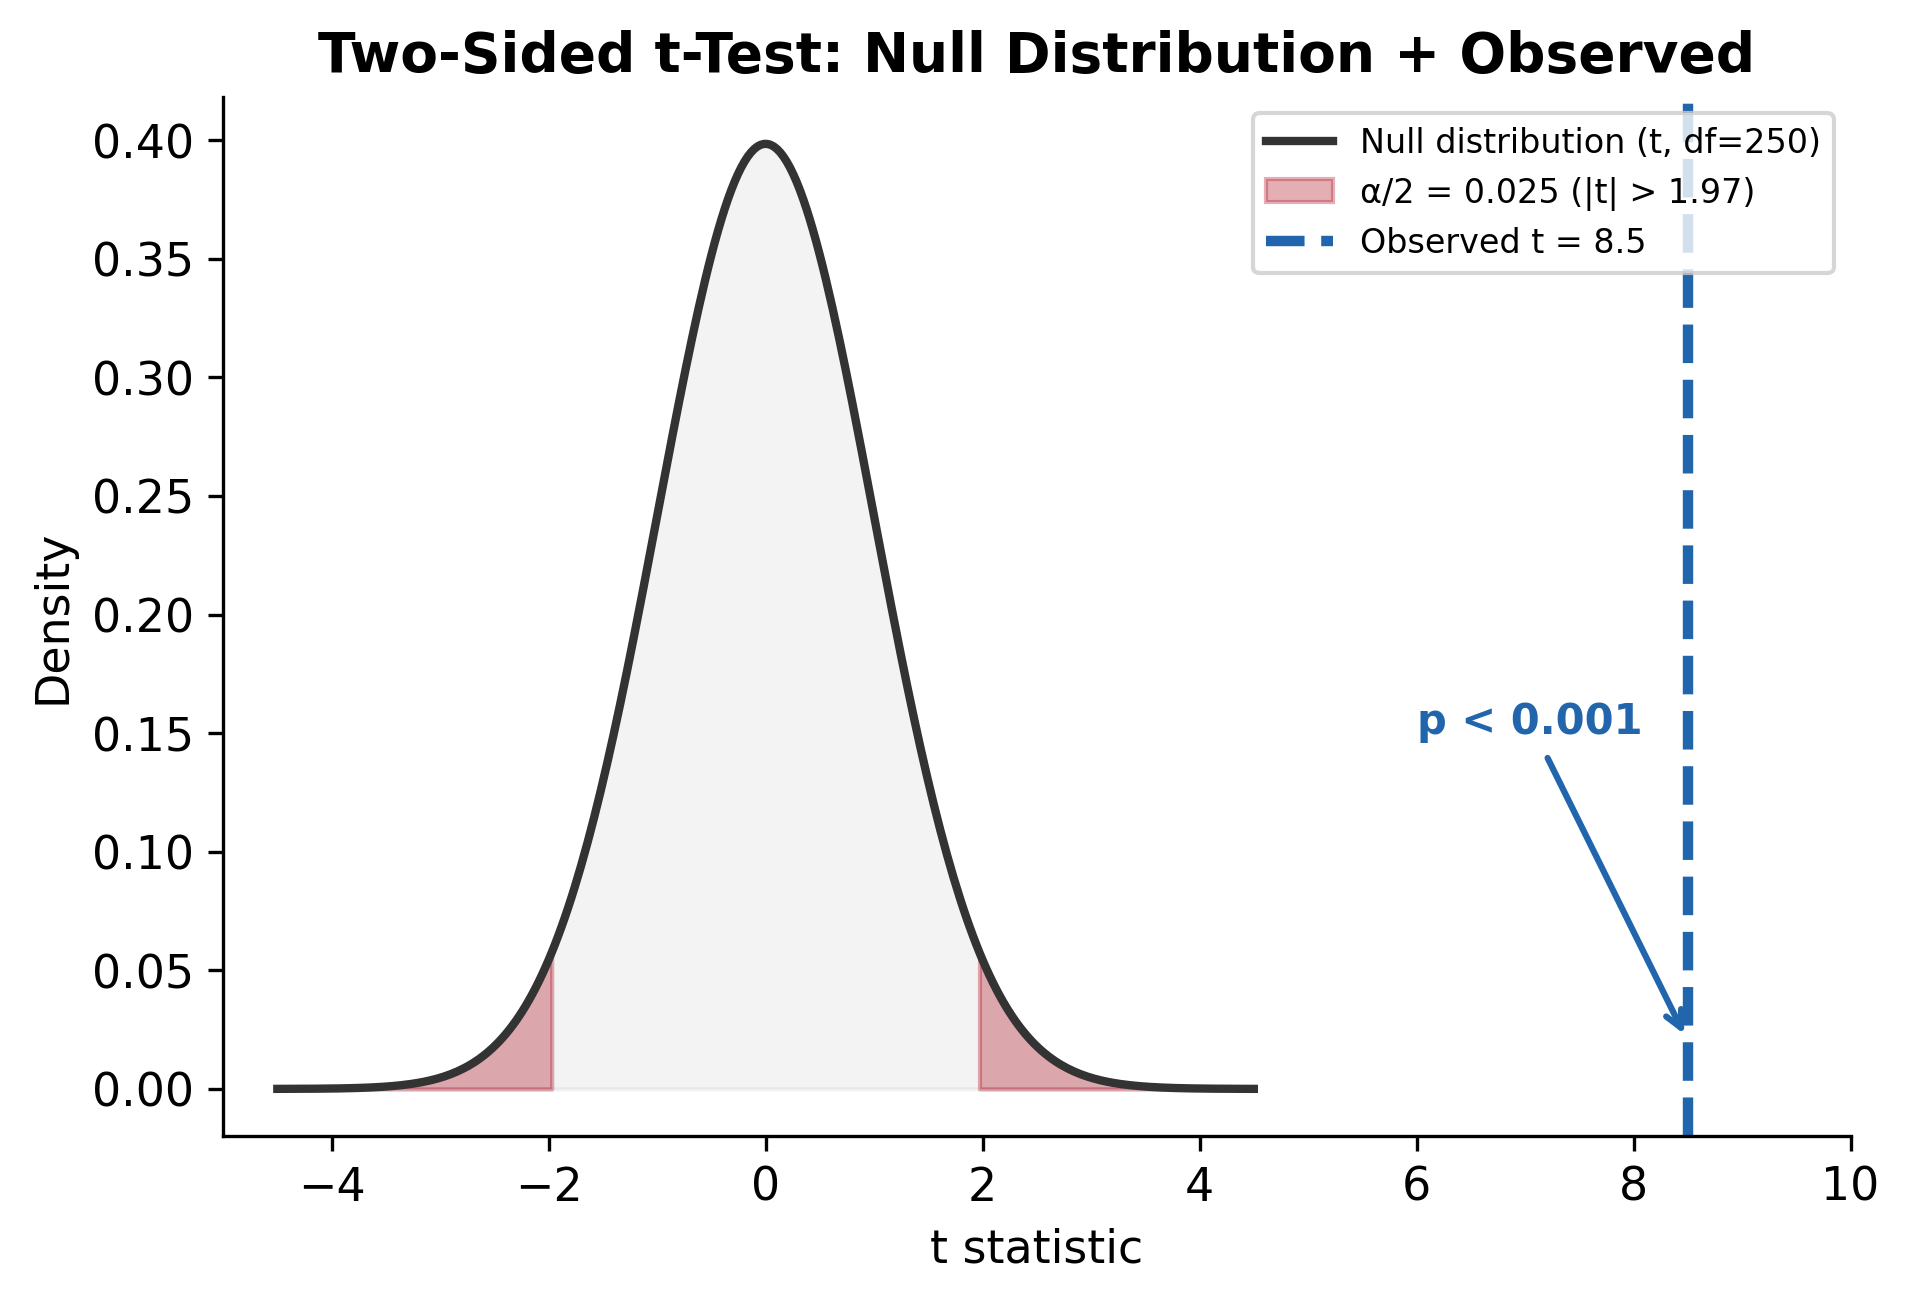
\includegraphics[width=0.72\textwidth]{m2_7_t_test_null.png}

\vspace{0.2cm}
\begin{exampleblock}{Data Insight}
    \scriptsize The grey curve is what $t$ would look like if $H_0$ were true. The observed $t = 8.5$ falls deep in the tail --- far from zero. The red shaded area is the rejection region ($\alpha = 0.05$, two-tailed). The $p$-value is the area beyond $|t_{\text{obs}}|$.
\end{exampleblock}
\end{frame}

% ── 184 ──
\begin{frame}{$p$-Value as Tail Area}
\smark{184/300}
\centering
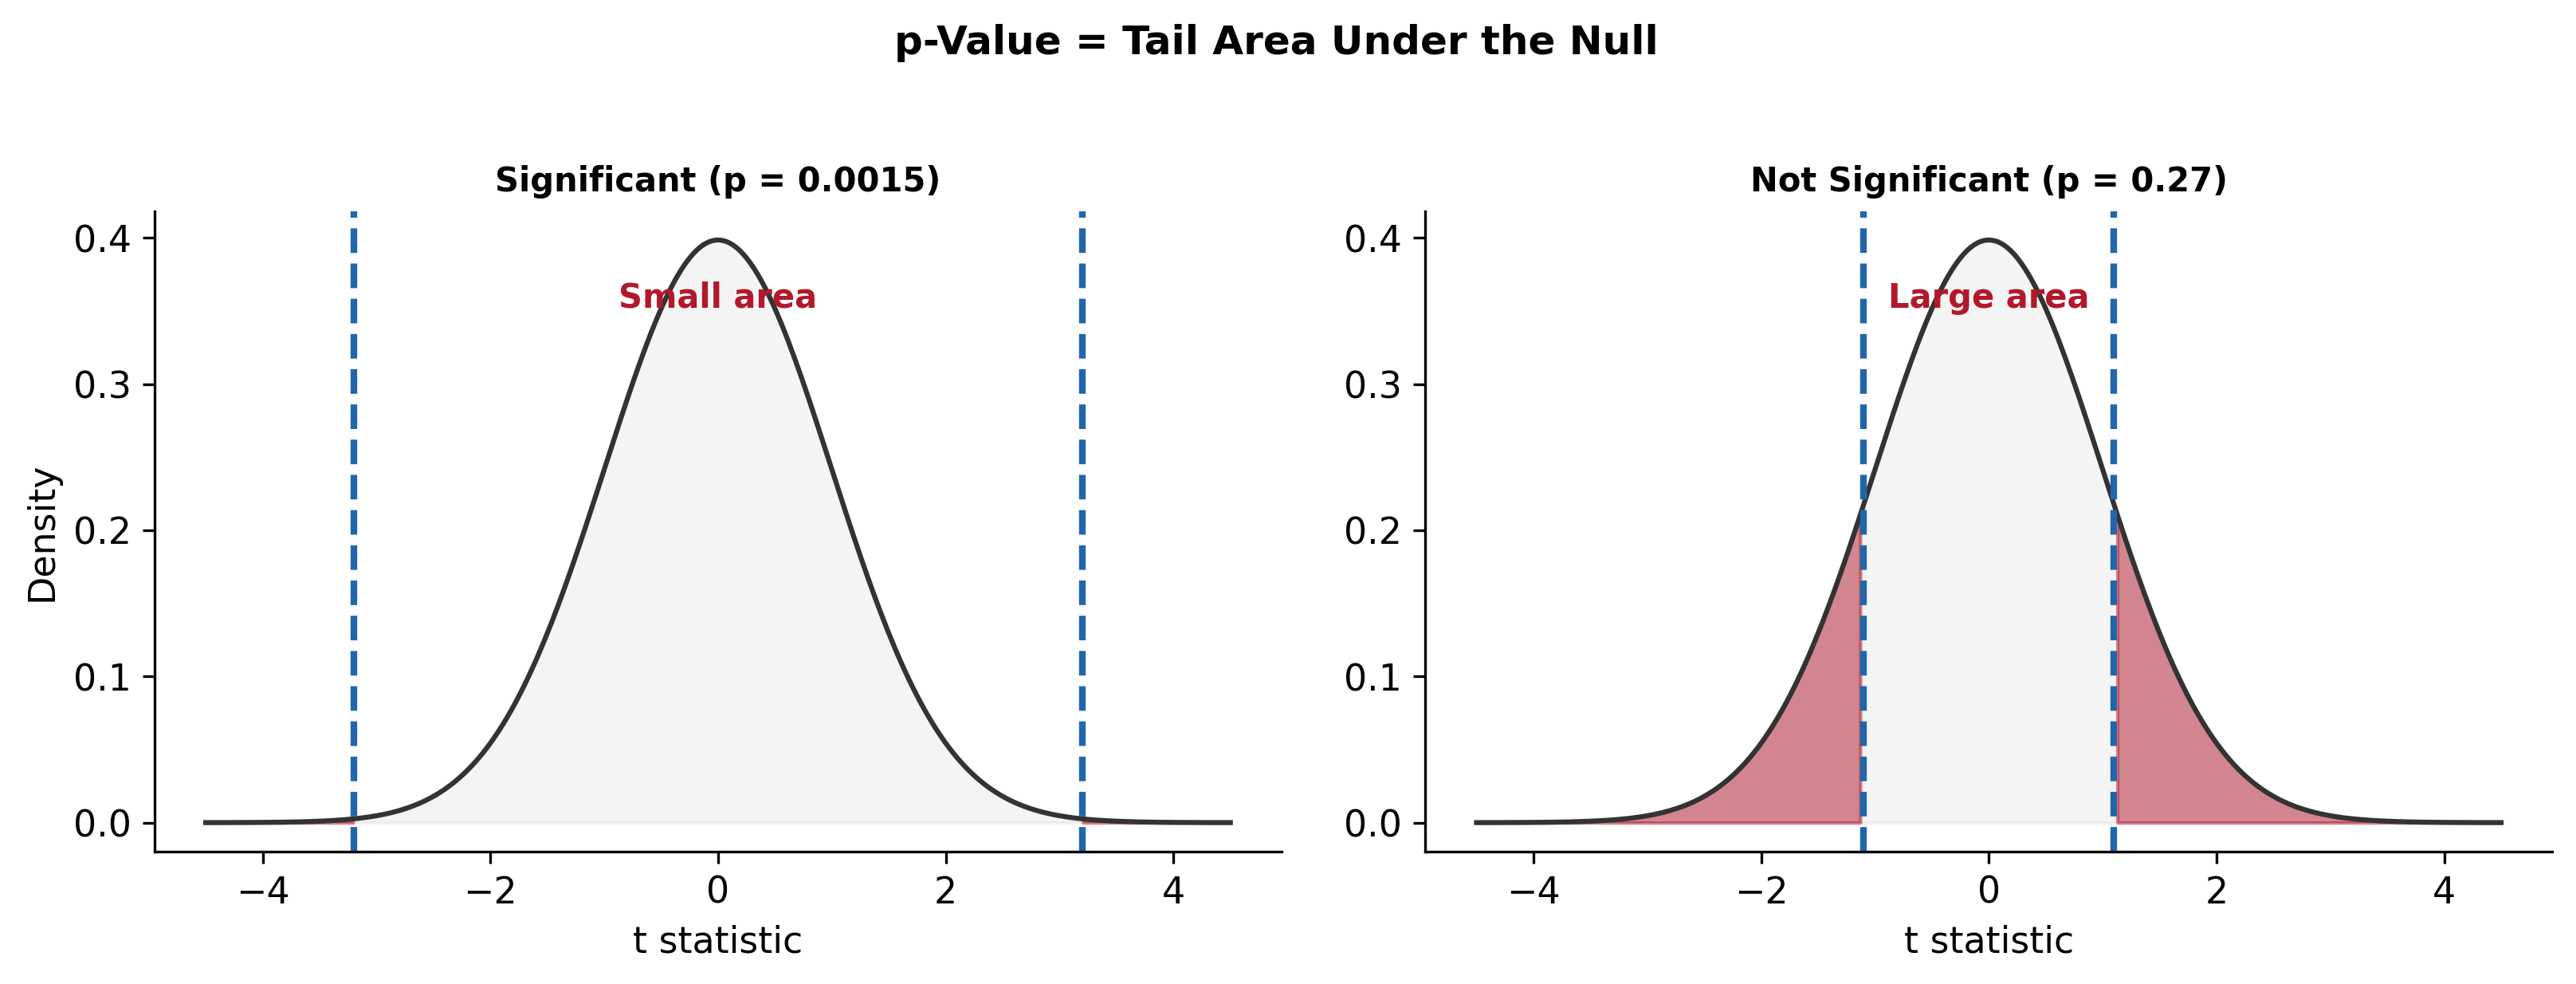
\includegraphics[width=0.88\textwidth]{m2_7_pvalue_area.png}

\vspace{0.2cm}
\begin{columns}[T]
\begin{column}{0.48\textwidth}
\begin{exampleblock}{Data Insight}
    \scriptsize Left: $t = 3.2$ yields a tiny tail area ($p = 0.0015$). Right: $t = 1.1$ yields a large tail area ($p = 0.27$). The $p$-value \textbf{is} the area, not a binary yes/no.
\end{exampleblock}
\end{column}
\begin{column}{0.48\textwidth}
\begin{alertblock}{Pro-Tip}
    \scriptsize $p = 0.049$ and $p = 0.051$ are practically identical. The $\alpha = 0.05$ threshold is a convention, not a law of nature. Visualizing the tail area makes this continuity visible.
\end{alertblock}
\end{column}
\end{columns}
\end{frame}

% ── 185 ──
\begin{frame}[fragile]{Null Distribution Plot --- Code}\smark{185/300}
\begin{columns}[T]
\begin{column}{0.48\textwidth}
\begin{lstlisting}[style=Rstyle]
# Compute test
t_result <- t.test(
  body_mass_g ~ species,
  data = filter(penguins,
    species %in%
      c("Adelie","Gentoo")))

# Plot null + observed
x <- seq(-5, 10, 0.01)
df_t <- t_result$parameter
ggplot(data.frame(x), aes(x)) +
  stat_function(fun=dt,
    args=list(df=df_t)) +
  geom_vline(
    xintercept=t_result$statistic,
    color="#2166AC", linewidth=1.5,
    linetype="dashed") +
  theme_minimal()
\end{lstlisting}
\end{column}
\begin{column}{0.48\textwidth}
\begin{lstlisting}[style=Pystyle]
from scipy.stats import ttest_ind, t

adelie = pen[pen.species=="Adelie"]\
    ["body_mass_g"]
gentoo = pen[pen.species=="Gentoo"]\
    ["body_mass_g"]
stat, pval = ttest_ind(adelie,gentoo)

x = np.linspace(-5, 10, 300)
ax.plot(x, t.pdf(x, df=250))
ax.axvline(abs(stat),
    color="#2166AC", linewidth=2,
    linestyle="--")
# Shade tail area
mask = x >= abs(stat)
ax.fill_between(x[mask],
    t.pdf(x[mask], df=250),
    alpha=0.3, color="#B2182B")
\end{lstlisting}
\end{column}
\end{columns}
\end{frame}

% ── 186 ──
\begin{frame}{Effect Size: Cohen's $d$ as Distribution Overlap}
\smark{186/300}
\centering
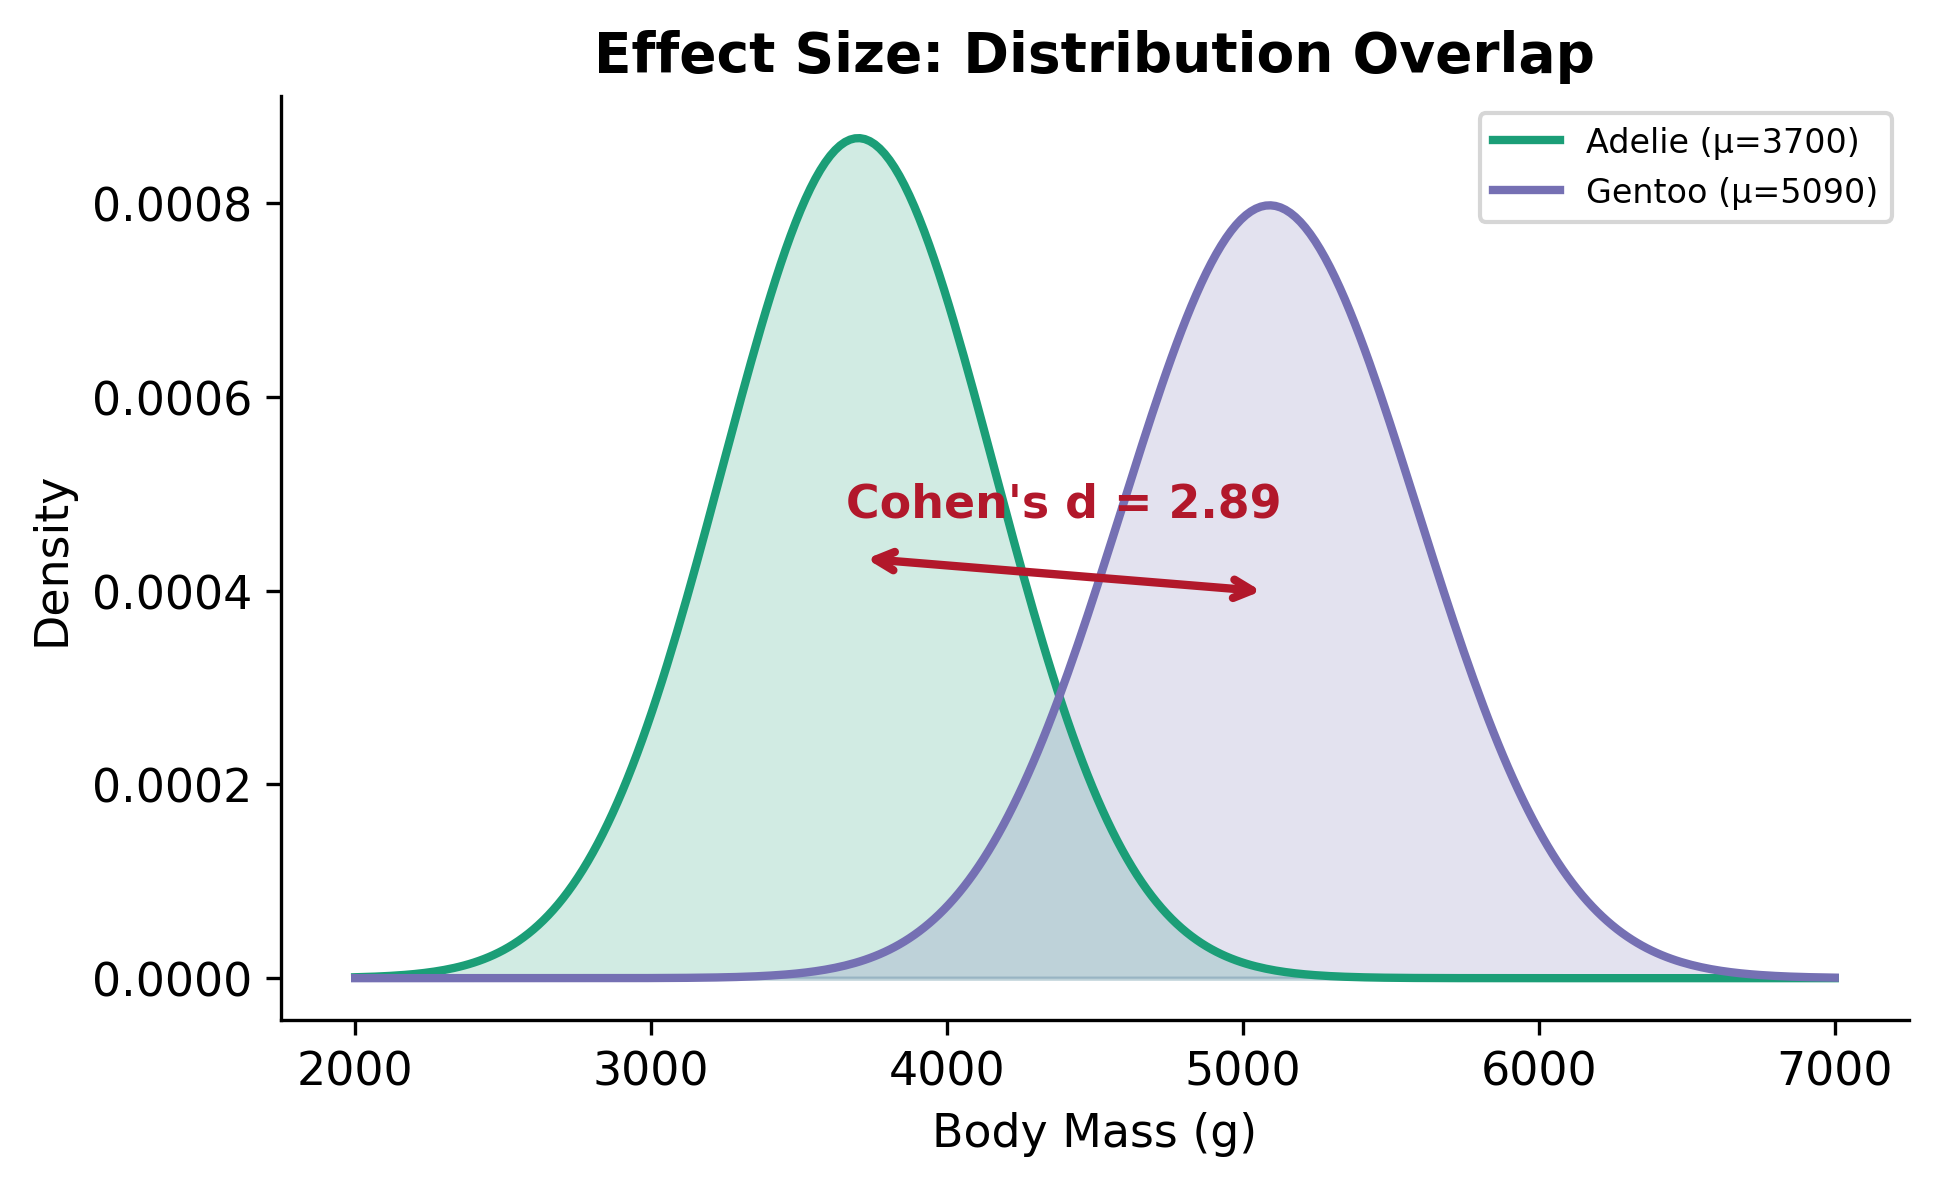
\includegraphics[width=0.72\textwidth]{m2_7_effect_size.png}

\vspace{0.2cm}
\begin{columns}[T]
\begin{column}{0.48\textwidth}
\centering\small
\begin{tabular}{@{}lr@{}}
    \toprule
    \textbf{Cohen's $d$} & \textbf{Interpretation} \\
    \midrule
    0.2 & Small \\
    0.5 & Medium \\
    0.8 & Large \\
    $>$1.2 & Very large \\
    \bottomrule
\end{tabular}
\end{column}
\begin{column}{0.48\textwidth}
\begin{exampleblock}{Data Insight}
    \scriptsize $d = 2.88$ for Adelie vs.\ Gentoo body mass: very large. The distributions barely overlap. This tells you more than $p < 0.001$ --- it tells you the \textbf{practical magnitude}.
\end{exampleblock}
\end{column}
\end{columns}
\end{frame}

% ── 187 ──
\begin{frame}[fragile]{Effect Size --- Code}\smark{187/300}
\begin{columns}[T]
\begin{column}{0.48\textwidth}
\begin{lstlisting}[style=Rstyle]
library(effectsize)

# Cohen's d
cohens_d(body_mass_g ~ species,
  data = filter(penguins,
    species %in%
      c("Adelie","Gentoo")))
# Returns d + 95% CI

# Visualize overlap
library(ggdist)
ggplot(pen_sub,
  aes(body_mass_g,
      fill=species)) +
  stat_slab(alpha=0.4) +
  theme_minimal()
\end{lstlisting}
\end{column}
\begin{column}{0.48\textwidth}
\begin{lstlisting}[style=Pystyle]
import pingouin as pg

# Cohen's d + CI
pg.compute_effsize(
    adelie, gentoo,
    eftype="cohen")

# Or manual
pooled_sd = np.sqrt(
    (adelie.std()**2 +
     gentoo.std()**2) / 2)
d = (gentoo.mean() -
     adelie.mean()) / pooled_sd

# Overlap visualization
xs = np.linspace(2000, 7000, 300)
ax.plot(xs, stats.norm.pdf(
    xs, adelie.mean(), adelie.std()))
ax.plot(xs, stats.norm.pdf(
    xs, gentoo.mean(), gentoo.std()))
\end{lstlisting}
\end{column}
\end{columns}
\end{frame}

% ── 188 ──
\begin{frame}{The Estimation Plot (Gardner--Altman)}
\smark{188/300}
\centering
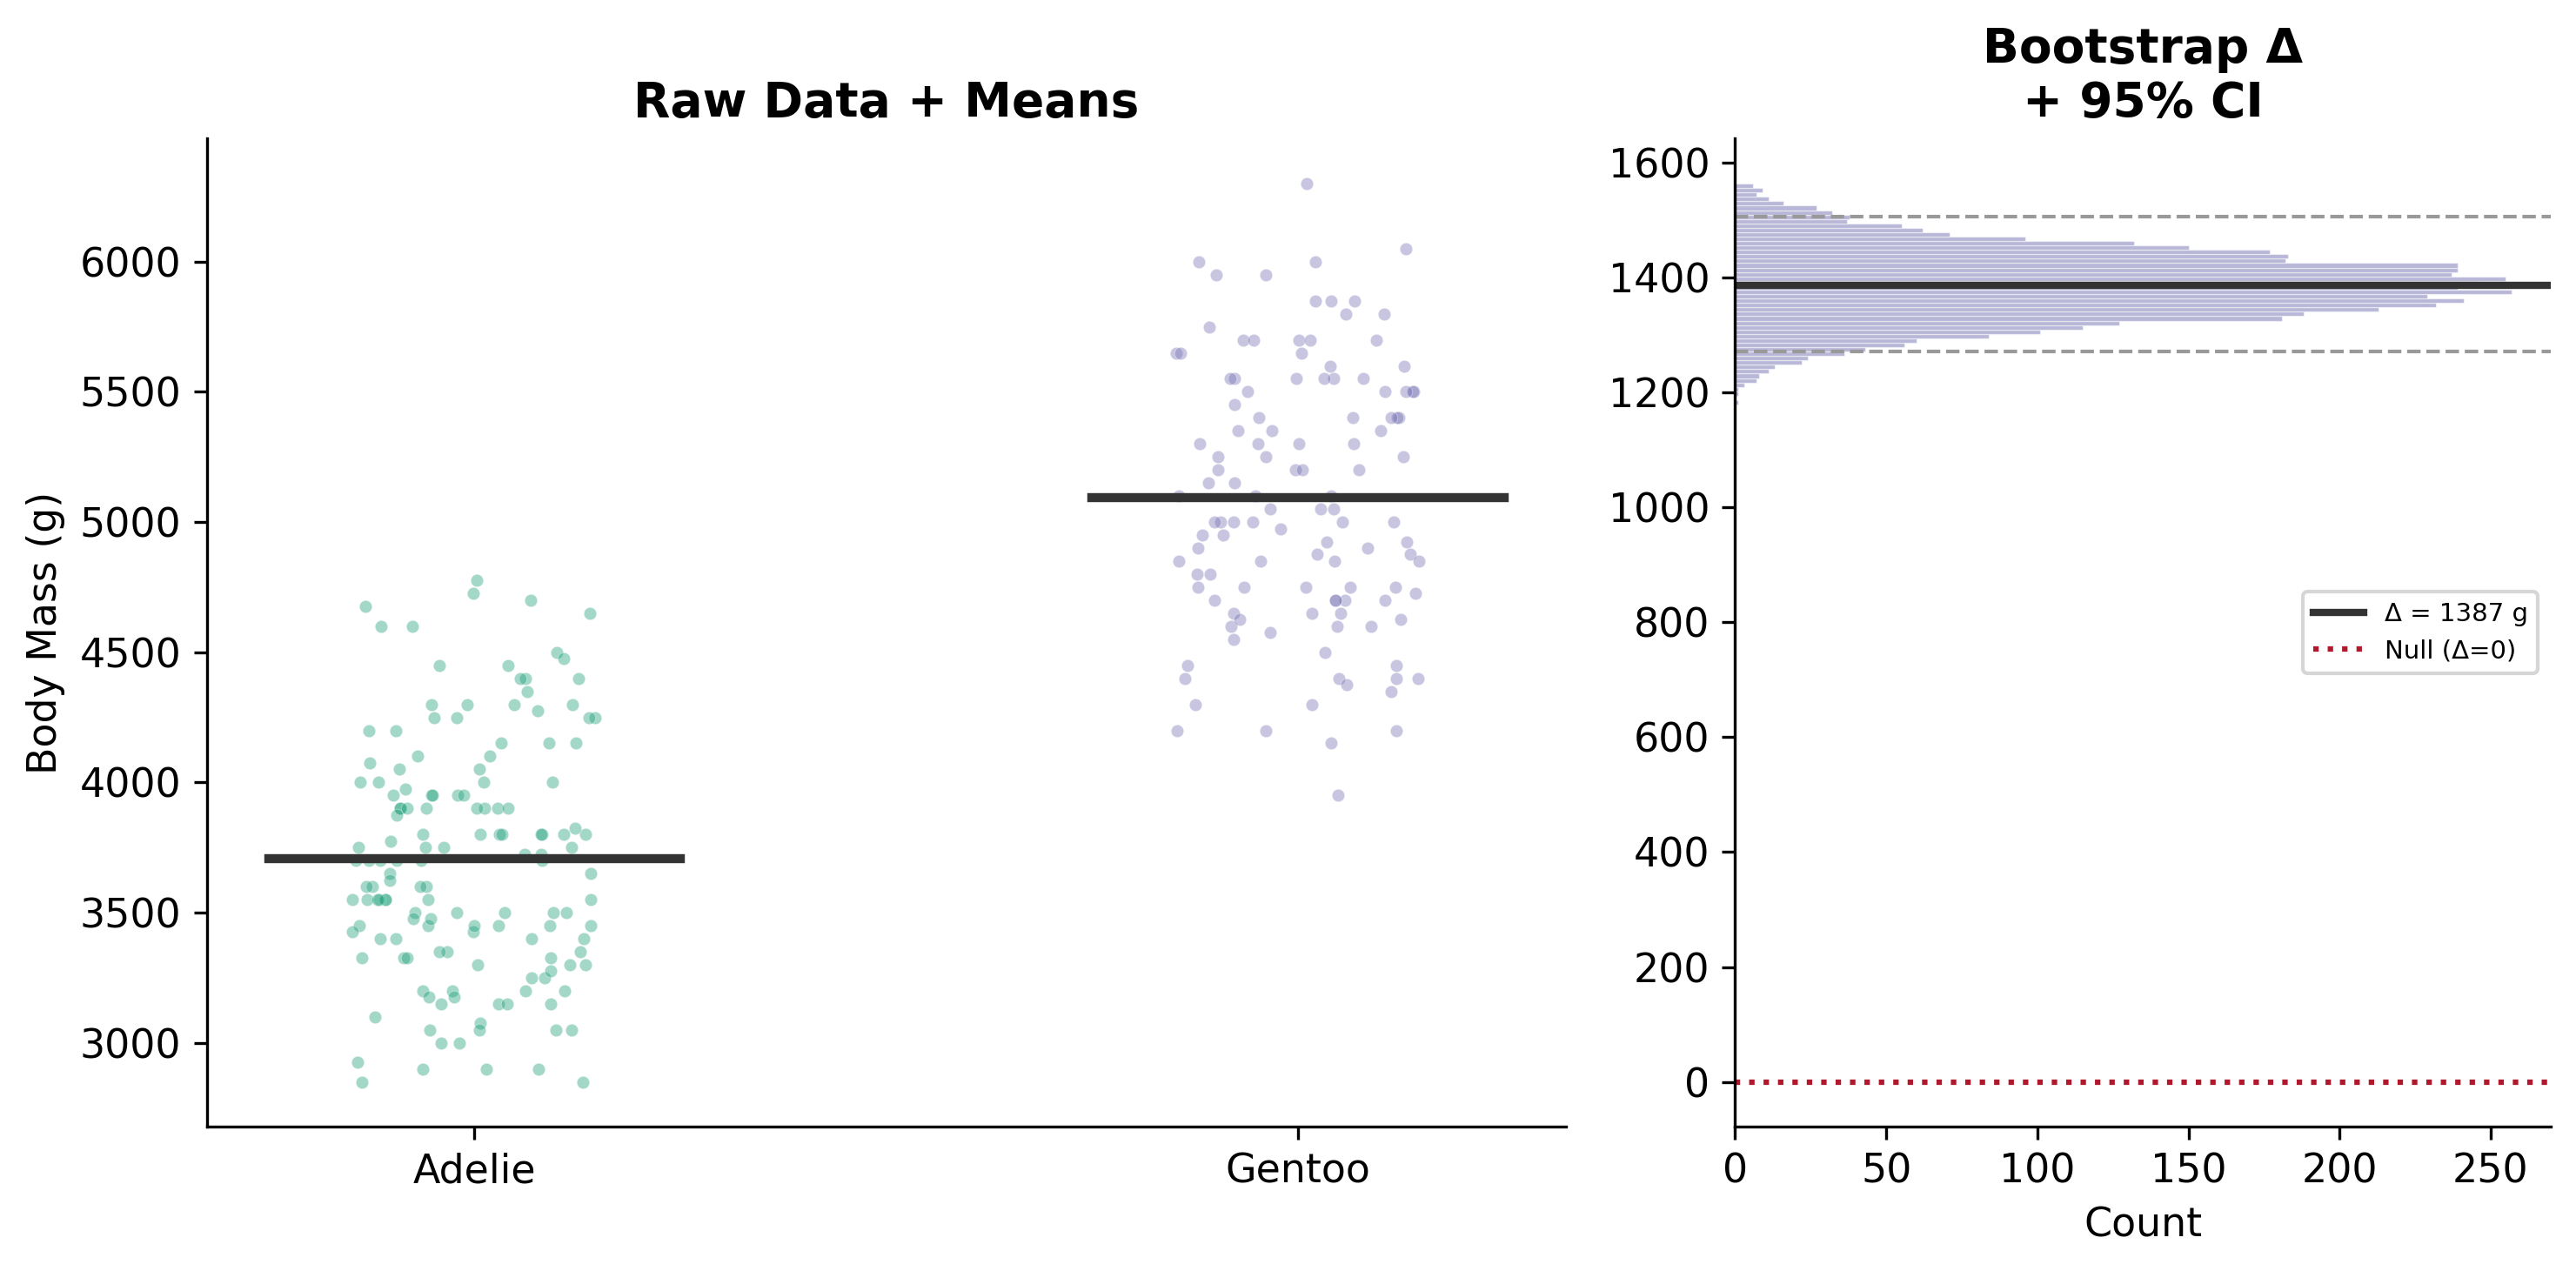
\includegraphics[width=0.78\textwidth]{m2_7_estimation_plot.png}

\vspace{0.2cm}
\begin{columns}[T]
\begin{column}{0.48\textwidth}
\begin{itemize}
    \item \textbf{Left panel}: raw data + means
    \item \textbf{Right panel}: bootstrap distribution of the difference $\Delta$
    \item The difference CI answers the scientific question directly
    \item No $p$-value needed
\end{itemize}
\end{column}
\begin{column}{0.48\textwidth}
\begin{exampleblock}{Data Insight}
    \scriptsize $\Delta = 1{,}387$\,g with 95\% CI $[1{,}269; 1{,}504]$. The entire CI is far from zero (red dotted line). This is more informative than ``$p < 0.001$.''
\end{exampleblock}
\end{column}
\end{columns}
\end{frame}

% ── 189 ──
\begin{frame}[fragile]{Estimation Plot --- \Rlang}\smark{189/300}
\begin{columns}[T]
\begin{column}{0.55\textwidth}
\begin{lstlisting}[style=Rstyle]
library(dabestr)

# Create analysis object
d <- dabest(penguins |>
  filter(species %in%
    c("Adelie","Gentoo")),
  x = species,
  y = body_mass_g,
  idx = c("Adelie","Gentoo"),
  paired = FALSE)

# Compute + plot mean difference
d |> mean_diff() |> plot()

# Also available:
# median_diff(), cohens_d(),
# hedges_g(), cliffs_delta()
\end{lstlisting}
\end{column}
\begin{column}{0.42\textwidth}
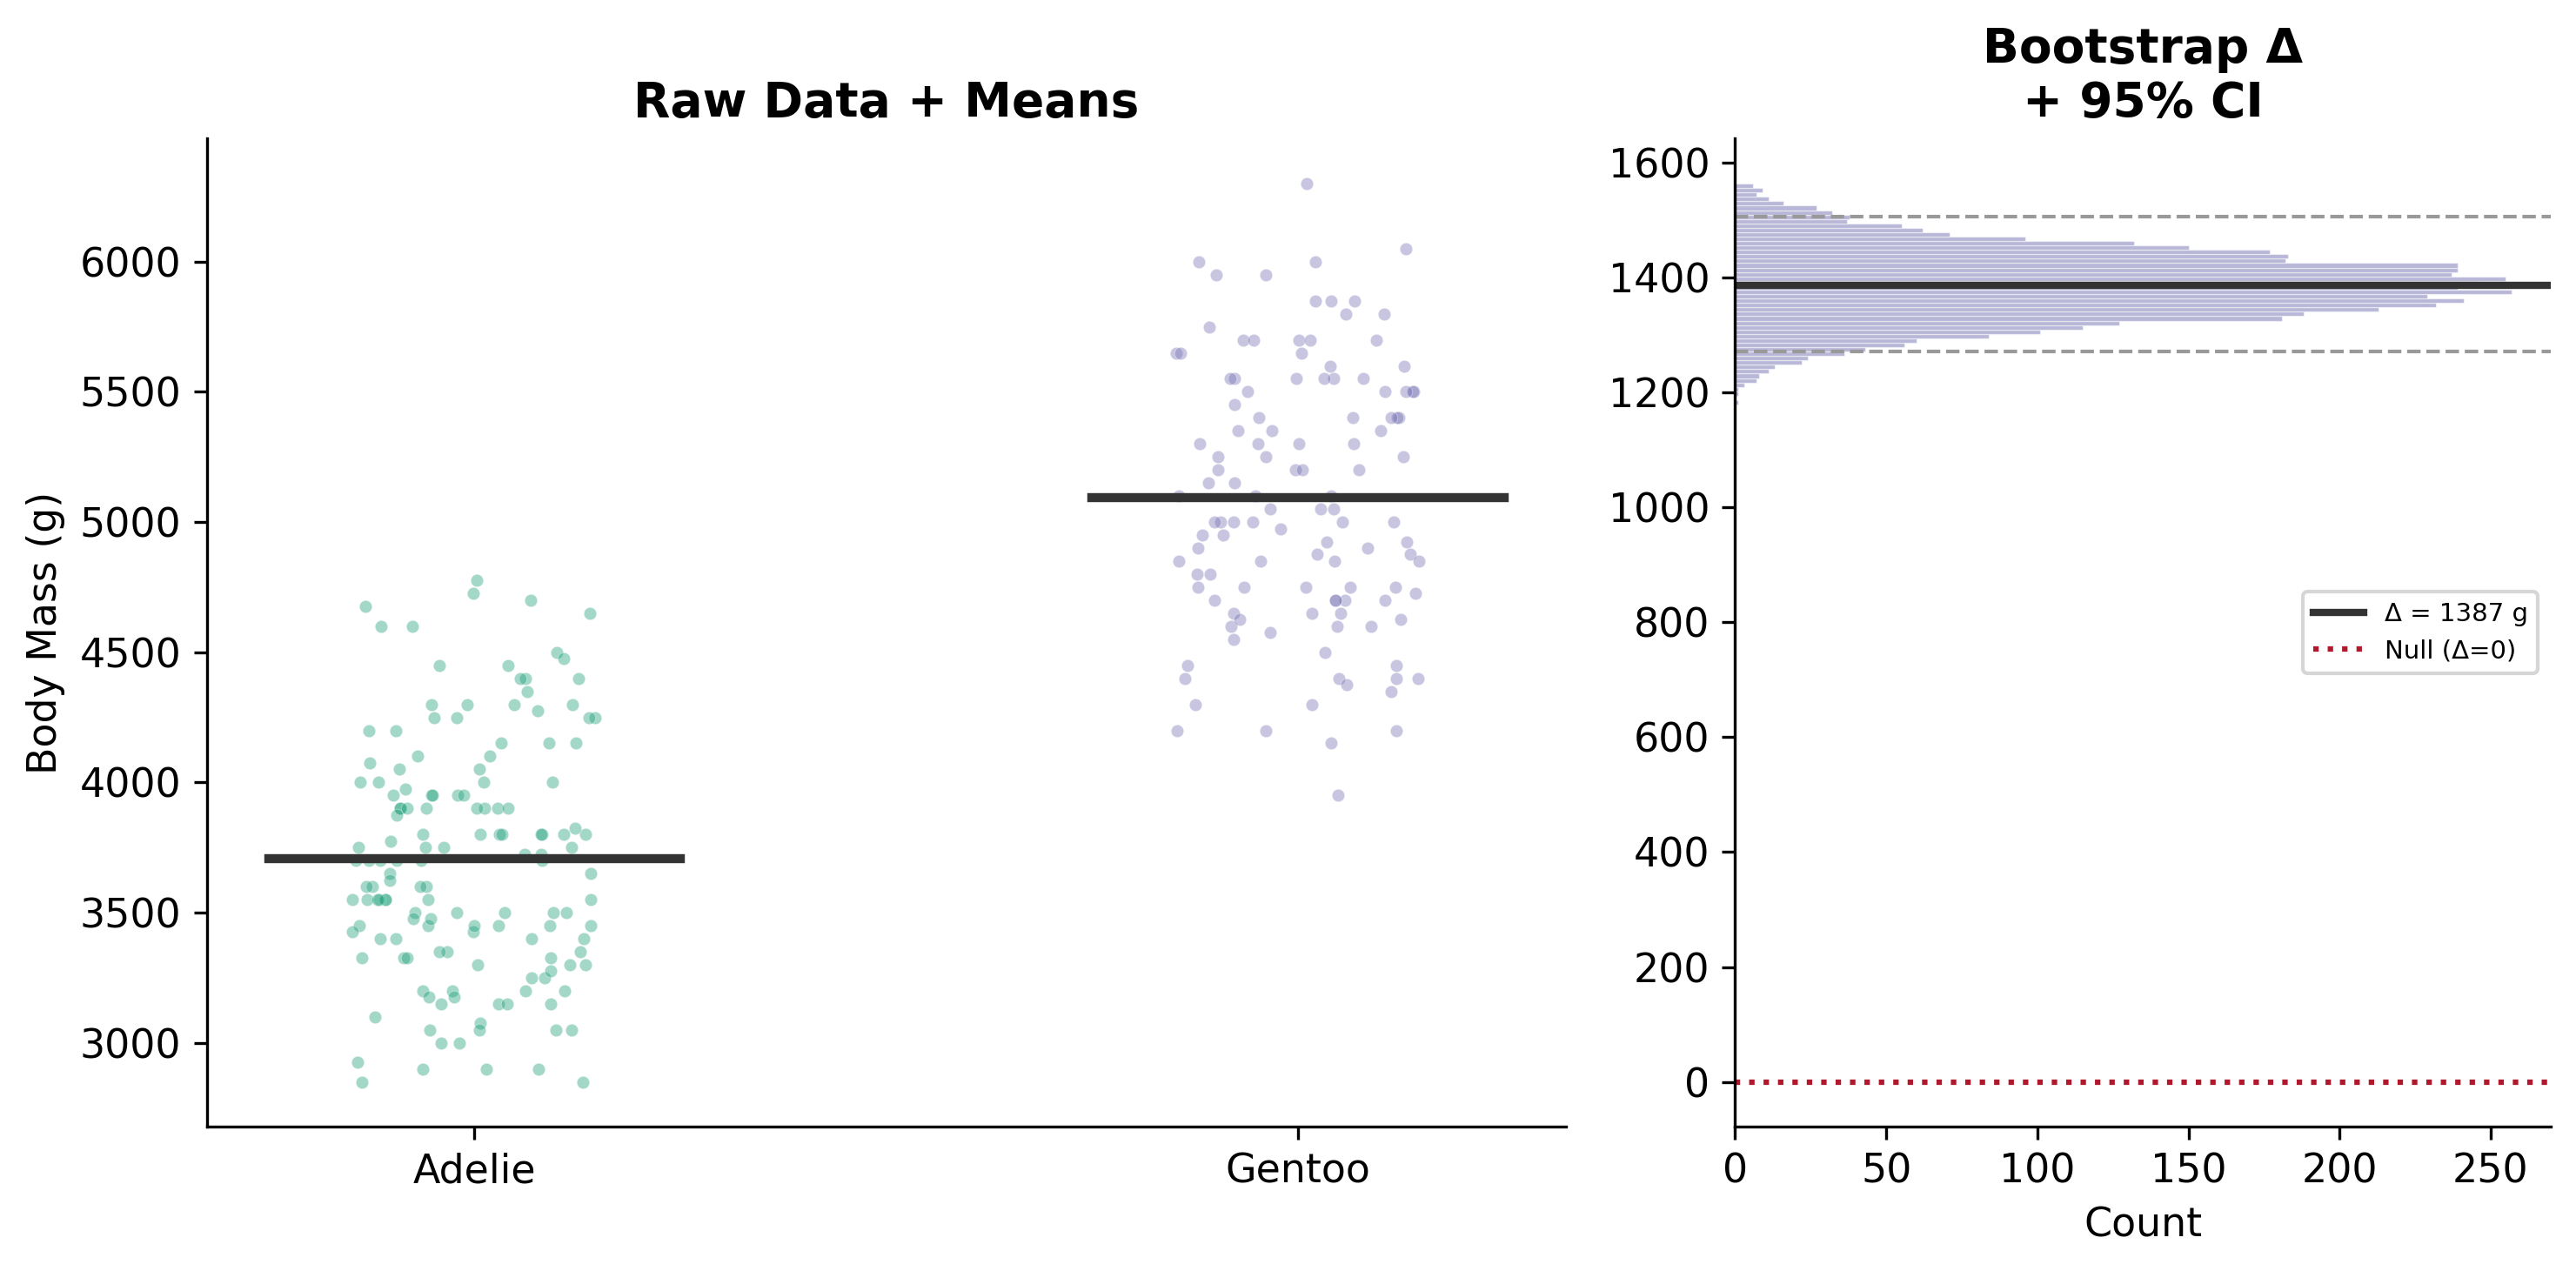
\includegraphics[width=\textwidth]{m2_7_estimation_plot.png}
\begin{alertblock}{Pro-Tip}
    \scriptsize \texttt{dabestr} (Data Analysis with Bootstrap-coupled ESTimation) produces publication-ready Gardner--Altman plots. One function call replaces a $t$-test table + bar chart.
\end{alertblock}
\end{column}
\end{columns}
\end{frame}

% ── 190 ──
\begin{frame}[fragile]{Estimation Plot --- \Python}\smark{190/300}
\begin{columns}[T]
\begin{column}{0.55\textwidth}
\begin{lstlisting}[style=Pystyle]
import dabest

# Create analysis
analysis = dabest.load(
    penguins.query(
      "species in "
      "['Adelie','Gentoo']"),
    x="species", y="body_mass_g",
    idx=("Adelie","Gentoo"))

# Compute + plot
analysis.mean_diff.plot()

# Access numeric results
print(analysis.mean_diff.results)
# difference, ci_low, ci_high,
# bca_low, bca_high, p_value
\end{lstlisting}
\end{column}
\begin{column}{0.42\textwidth}
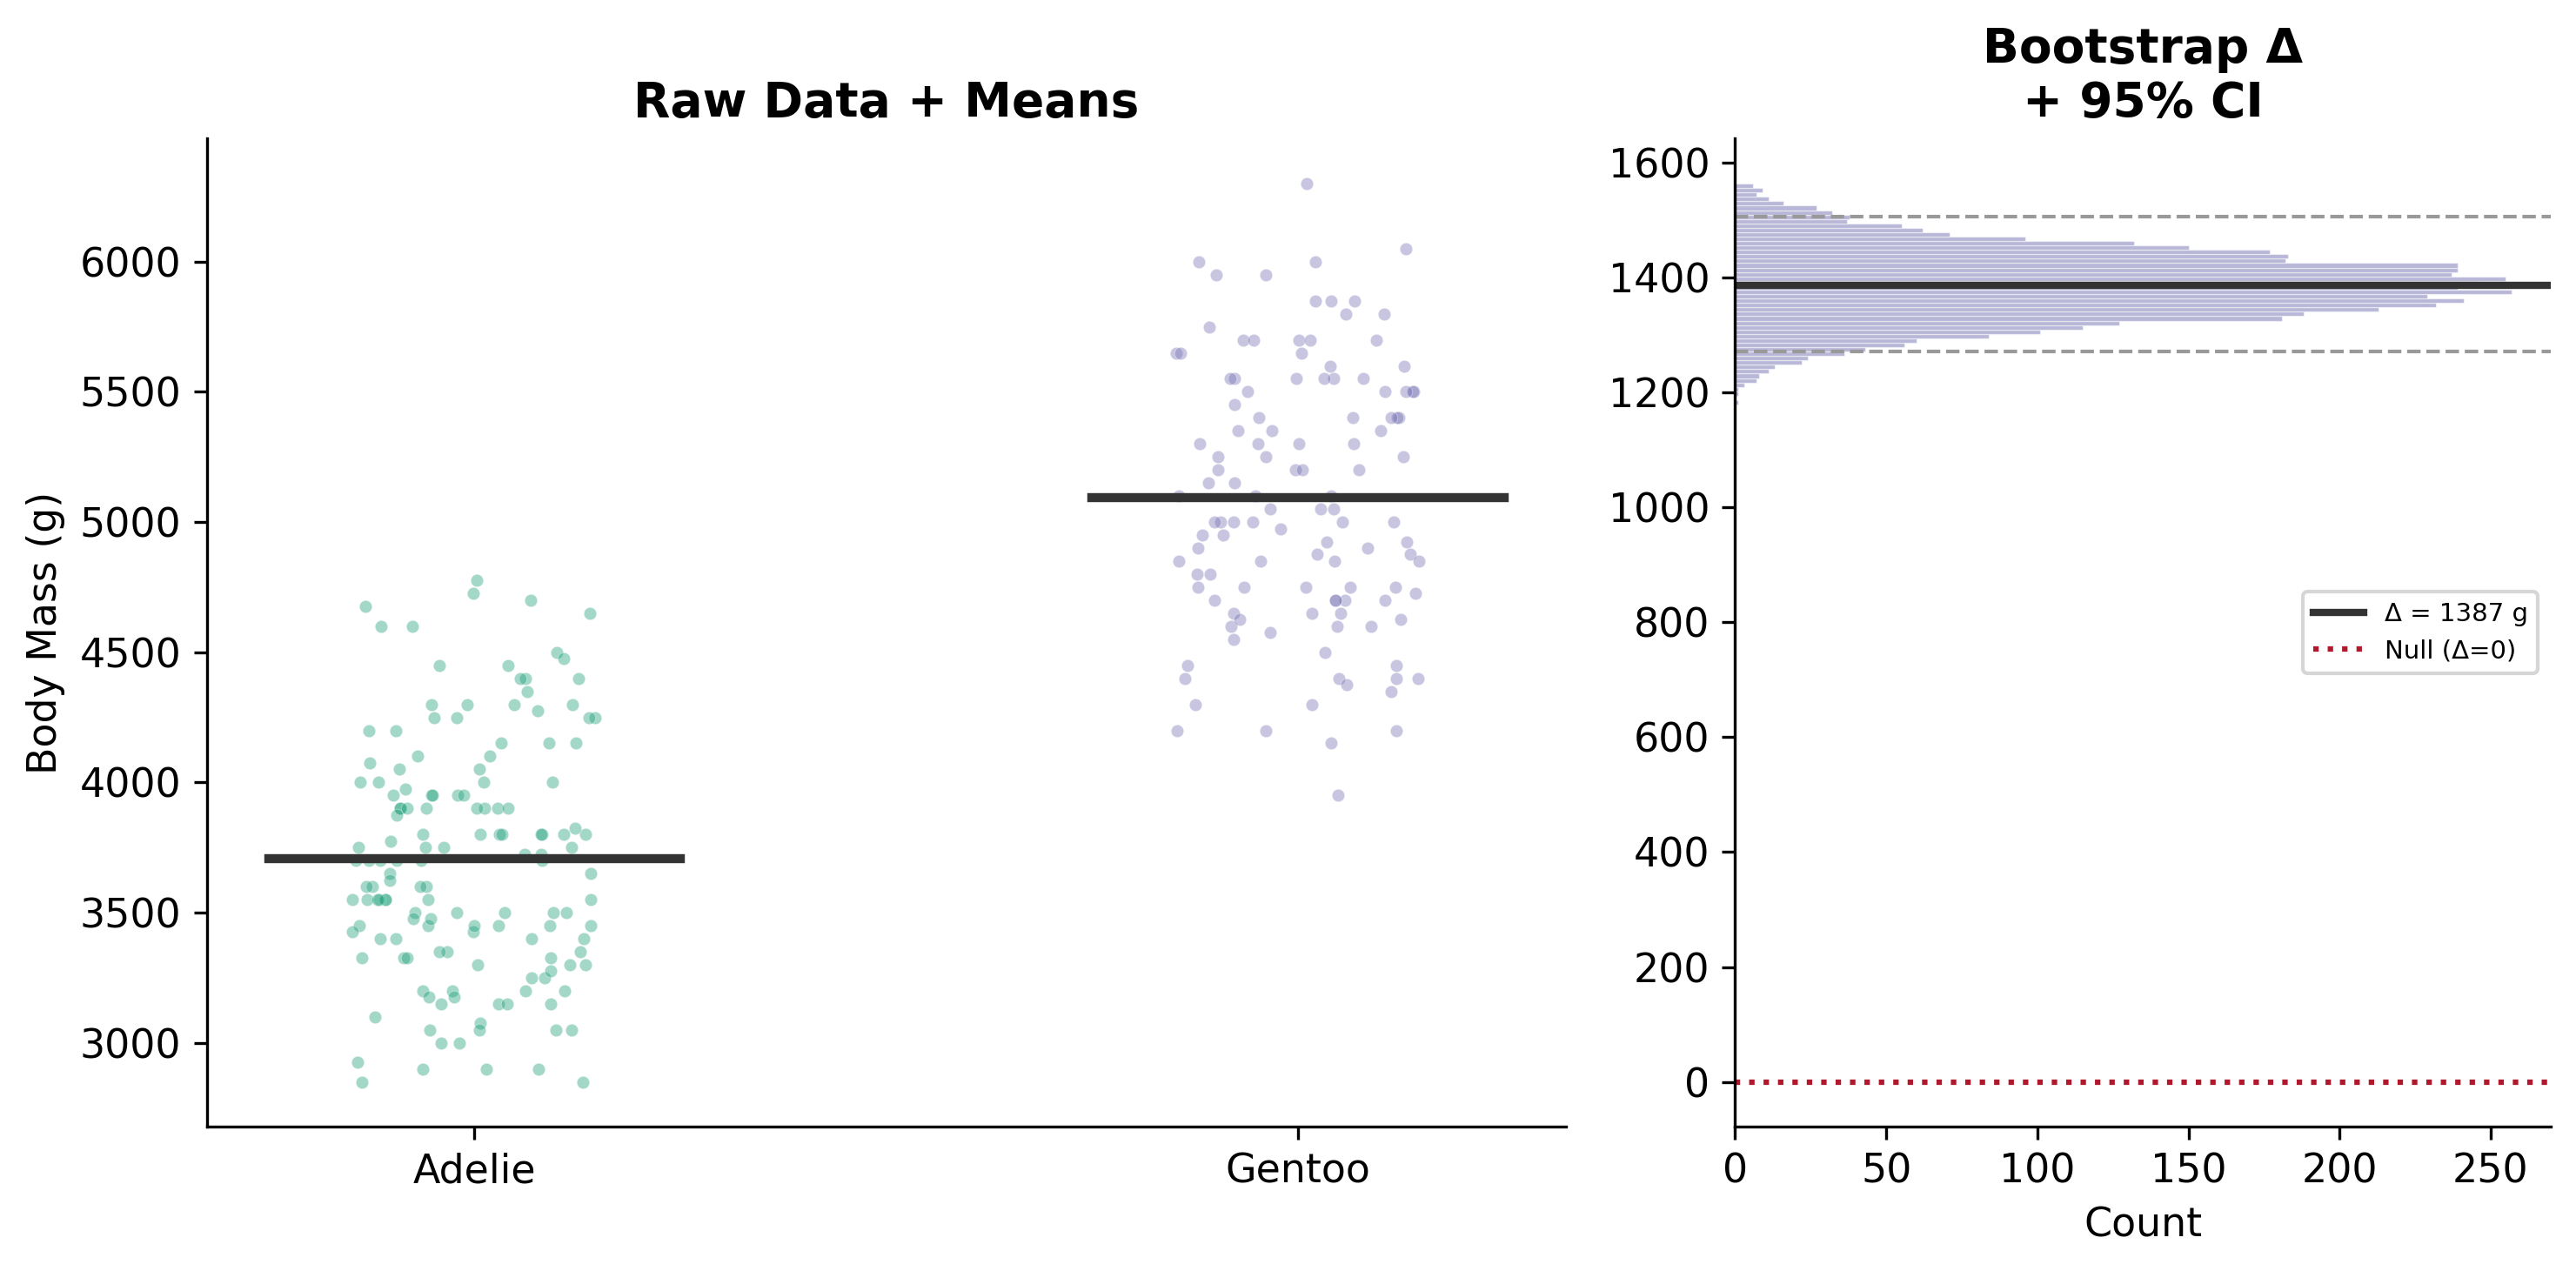
\includegraphics[width=\textwidth]{m2_7_estimation_plot.png}
\begin{exampleblock}{Data Insight}
    \scriptsize \texttt{dabest} is available in both R and Python with nearly identical APIs. It computes BCa (bias-corrected accelerated) bootstrap CIs --- more accurate than percentile CIs for small $n$.
\end{exampleblock}
\end{column}
\end{columns}
\end{frame}

% ── 191 ──
\begin{frame}{Significance Brackets}
\smark{191/300}
\centering
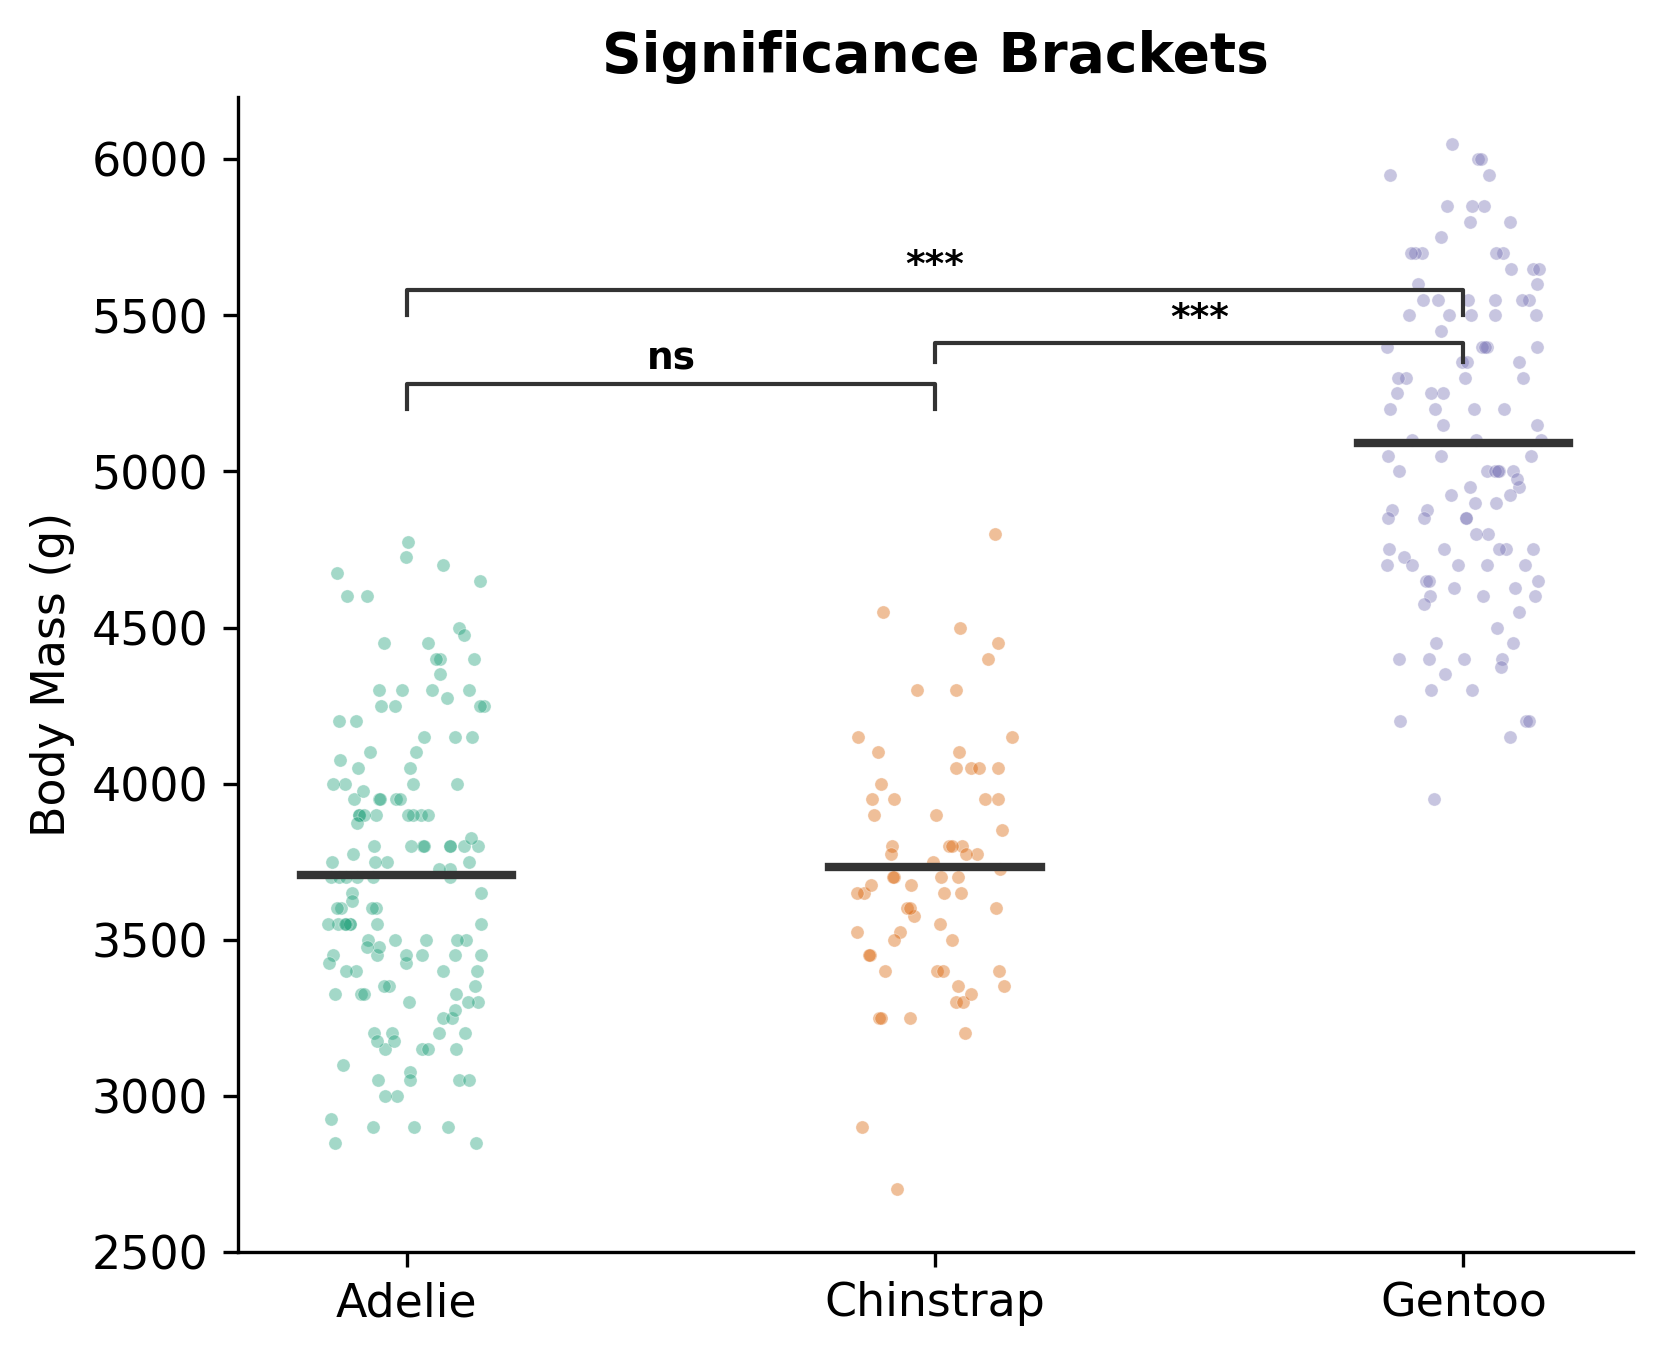
\includegraphics[width=0.55\textwidth]{m2_7_sig_brackets.png}

\vspace{0.2cm}
\begin{columns}[T]
\begin{column}{0.48\textwidth}
\begin{itemize}
    \item Horizontal bracket connecting two groups
    \item Stars or $p$-value annotated above
    \item Convention: * $p<0.05$, ** $p<0.01$, *** $p<0.001$, ns = not significant
\end{itemize}
\end{column}
\begin{column}{0.48\textwidth}
\begin{alertblock}{Pro-Tip}
    \scriptsize Brackets are overused and under-informative. A $p$-value star tells you \textbf{nothing} about effect magnitude. Prefer estimation plots or coefficient plots. Use brackets only when journal style demands it.
\end{alertblock}
\end{column}
\end{columns}
\end{frame}

% ── 192 ──
\begin{frame}[fragile]{Significance Brackets --- Code}\smark{192/300}
\begin{columns}[T]
\begin{column}{0.48\textwidth}
\begin{lstlisting}[style=Rstyle]
library(ggpubr)

ggplot(penguins,
  aes(species, body_mass_g)) +
  geom_boxplot(aes(fill=species),
    alpha=0.4) +
  stat_compare_means(
    comparisons = list(
      c("Adelie","Gentoo"),
      c("Chinstrap","Gentoo"),
      c("Adelie","Chinstrap")),
    method = "t.test",
    label = "p.signif") +
  theme_minimal()

# label options:
# "p.signif" = stars
# "p.format" = numeric p
\end{lstlisting}
\end{column}
\begin{column}{0.48\textwidth}
\begin{lstlisting}[style=Pystyle]
# statannotations package
from statannotations.Annotator \
    import Annotator

fig, ax = plt.subplots()
sns.boxplot(data=penguins,
    x="species", y="body_mass_g",
    ax=ax)

pairs = [("Adelie","Gentoo"),
         ("Chinstrap","Gentoo"),
         ("Adelie","Chinstrap")]
annot = Annotator(ax, pairs,
    data=penguins, x="species",
    y="body_mass_g")
annot.configure(test="t-test_ind",
    text_format="star")
annot.apply_and_annotate()
\end{lstlisting}
\end{column}
\end{columns}
\end{frame}

% ── 193 ──
\begin{frame}{Why Stars Are Not Enough}
\smark{193/300}
\begin{columns}[T]
\begin{column}{0.50\textwidth}
\begin{itemize}
    \item *** means $p < 0.001$ --- but says \textbf{nothing} about:
    \item How \textbf{large} the effect is (Cohen's $d$?)
    \item How \textbf{precise} the estimate is (CI width?)
    \item Whether the effect is \textbf{practically} meaningful
    \item $n = 10{,}000$ will make tiny effects ``significant''
\end{itemize}
\end{column}
\begin{column}{0.47\textwidth}
\begin{exampleblock}{Data Insight}
    \scriptsize Cumming (2014): ``We should not dichotomize into significant/not significant. We should estimate, with uncertainty.'' The ASA Statement on $p$-values (Wasserstein \& Lazar, 2016) agrees: ``Scientific conclusions should not be based only on whether a $p$-value passes a specific threshold.''
\end{exampleblock}
\end{column}
\end{columns}
\end{frame}

% ── 194 ──
\begin{frame}{The New Statistics: Estimation Over Testing}
\smark{194/300}
\centering\small
\begin{tabular}{@{}lll@{}}
    \toprule
    \textbf{Old Approach} & \textbf{New Approach} & \textbf{Visualization} \\
    \midrule
    $p$-value (binary)    & Effect size + CI (continuous) & Estimation plot \\
    Bar + error bar       & Strip + mean $\pm$ CI         & Hybrid / raincloud \\
    Star brackets         & Difference CI                 & Gardner--Altman \\
    ``Significant''       & ``$\Delta = 1{,}387 \pm 118$ g''   & Forest / coefficient plot \\
    NHST table            & Visual summary                & \texttt{dabestr} / \texttt{ggdist} \\
    \bottomrule
\end{tabular}

\vspace{0.3cm}
\begin{exampleblock}{Data Insight}
    \scriptsize The shift from NHST to estimation statistics is endorsed by the APA (7th ed.), Nature Methods, eLife, and the ASA. Visualization is the primary medium for this shift --- tables of $p$-values cannot convey what estimation plots do.
\end{exampleblock}
\end{frame}

% ── 195 ──
\begin{frame}{Volcano Plots: High-Dimensional Testing}
\smark{195/300}
\centering
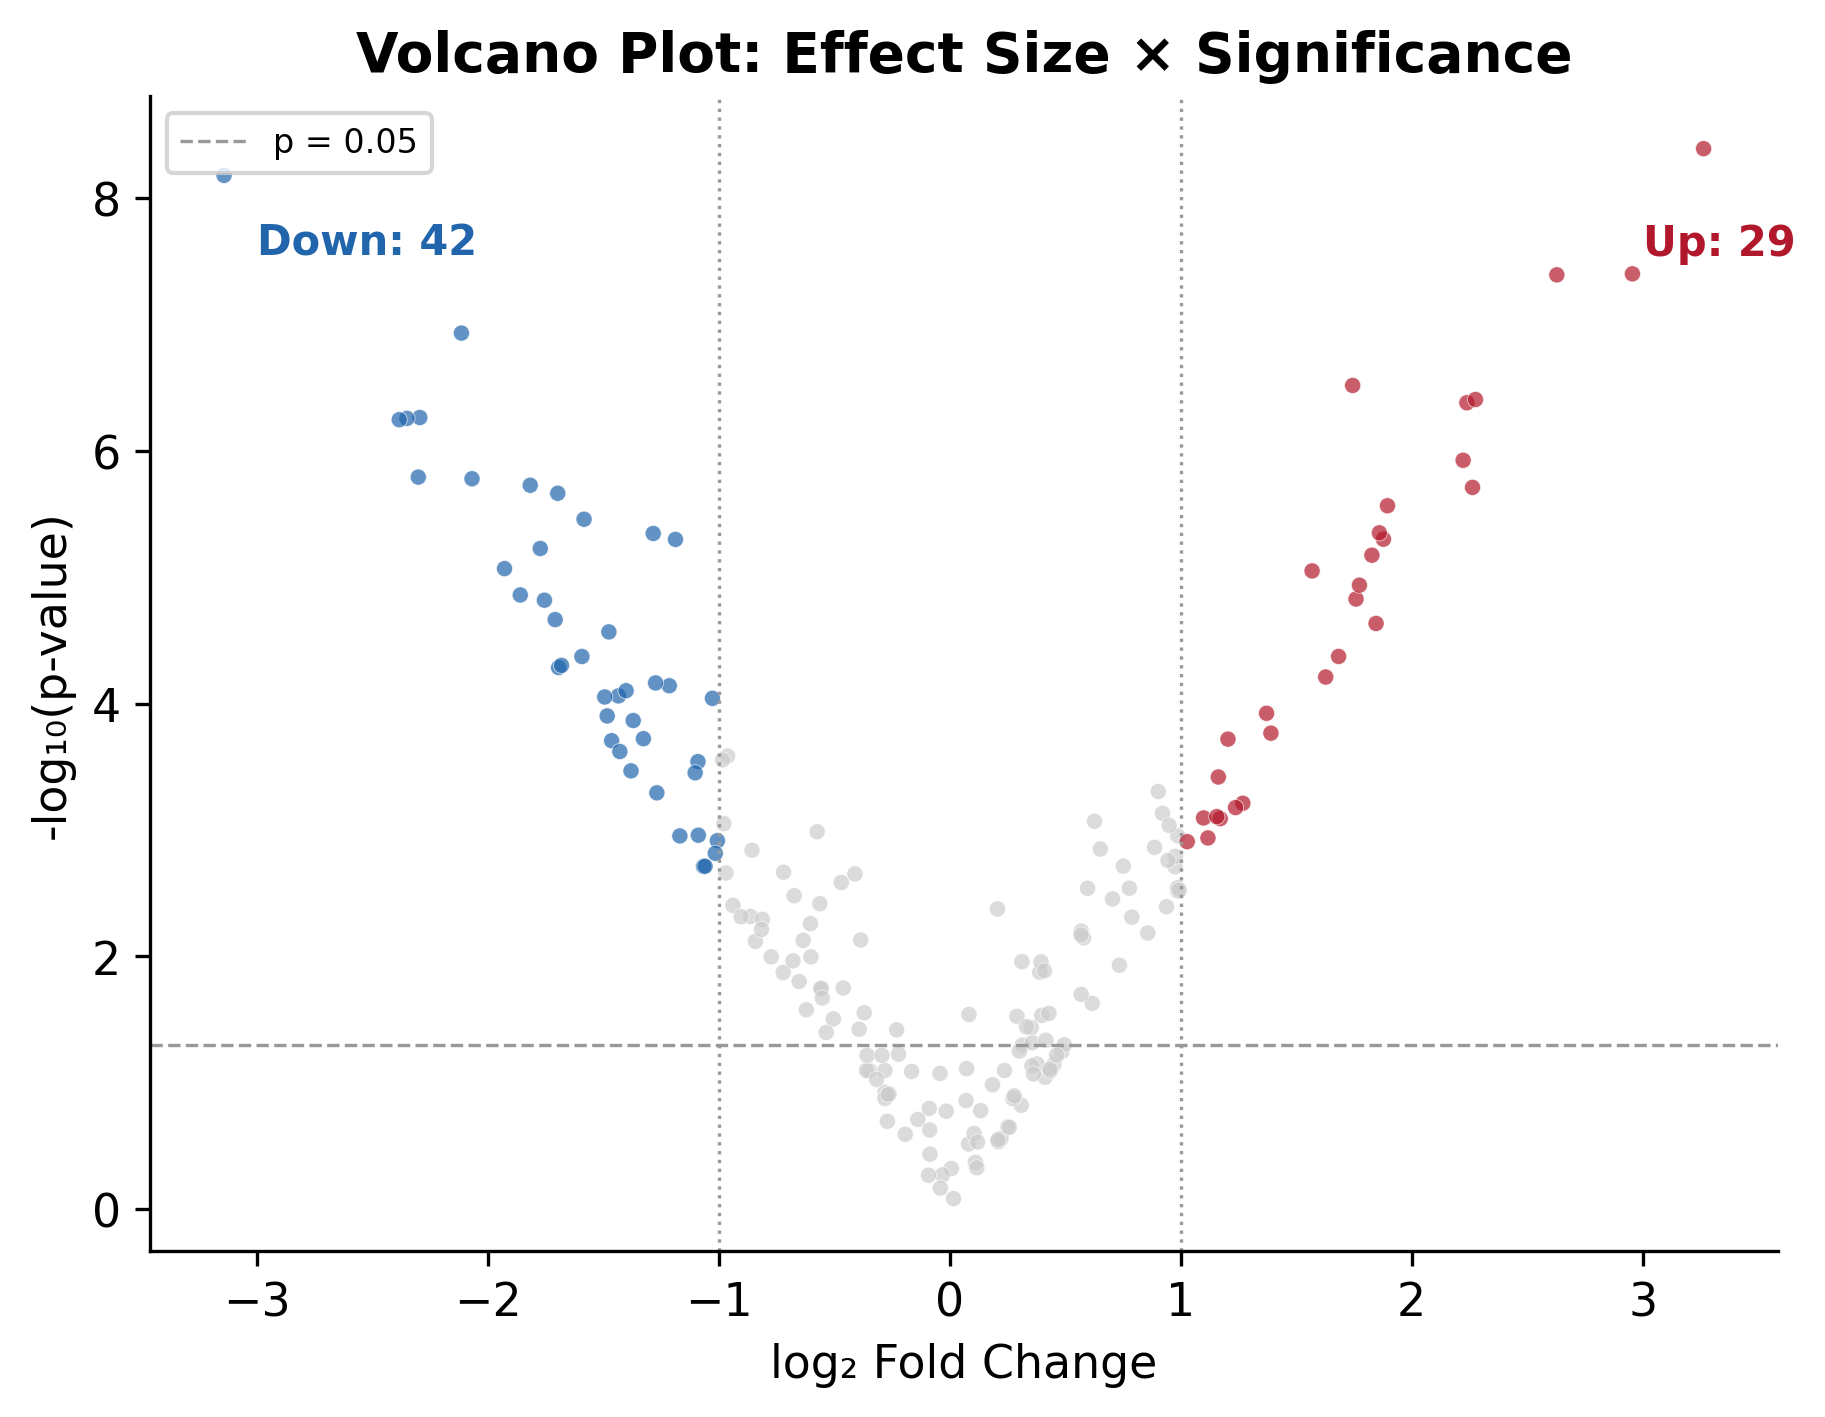
\includegraphics[width=0.68\textwidth]{m2_7_volcano.png}

\vspace{0.2cm}
\begin{columns}[T]
\begin{column}{0.48\textwidth}
\begin{itemize}
    \item $x$ = effect size (log$_2$ fold change)
    \item $y$ = significance ($-\log_{10} p$)
    \item Upper corners = large \textbf{and} significant
    \item Center / bottom = small or non-significant
    \item Standard in genomics, proteomics, metabolomics
\end{itemize}
\end{column}
\begin{column}{0.48\textwidth}
\begin{exampleblock}{Data Insight}
    \scriptsize The volcano plot forces you to consider \textbf{both} dimensions: a gene that is highly significant ($p < 10^{-10}$) but with fold change $< 1.5\times$ may not be biologically interesting. Points in the upper corners are the priority.
\end{exampleblock}
\end{column}
\end{columns}
\end{frame}

% ── 196 ──
\begin{frame}[fragile]{Volcano Plot --- Code}\smark{196/300}
\begin{columns}[T]
\begin{column}{0.48\textwidth}
\begin{lstlisting}[style=Rstyle]
library(EnhancedVolcano)

EnhancedVolcano(results_df,
  lab = results_df$gene,
  x = "log2FoldChange",
  y = "pvalue",
  pCutoff = 0.05,
  FCcutoff = 1.0,
  title = "Differential Expression")

# Manual with ggplot2
ggplot(df, aes(log2FC,
    -log10(pvalue))) +
  geom_point(aes(color=sig),
    size=1, alpha=0.6) +
  geom_hline(yintercept=
    -log10(0.05), linetype="--")+
  geom_vline(xintercept=c(-1,1),
    linetype=":")
\end{lstlisting}
\end{column}
\begin{column}{0.48\textwidth}
\begin{lstlisting}[style=Pystyle]
# Manual in matplotlib
sig = (neg_log_p > -np.log10(0.05))\
    & (np.abs(log2fc) > 1)
colors = np.where(
    sig & (log2fc > 0), "#B2182B",
    np.where(
      sig & (log2fc < 0), "#2166AC",
      "#CCCCCC"))

ax.scatter(log2fc, neg_log_p,
    c=colors, s=15, alpha=0.7)
ax.axhline(-np.log10(0.05),
    linestyle="--", color="#999")
ax.axvline(1, linestyle=":")
ax.axvline(-1, linestyle=":")
ax.set_xlabel("log2 Fold Change")
ax.set_ylabel("-log10(p)")
\end{lstlisting}
\end{column}
\end{columns}
\end{frame}

% ── 197 ──
\begin{frame}{Multiple Testing Correction: Visual Impact}
\smark{197/300}
\begin{columns}[T]
\begin{column}{0.50\textwidth}
\begin{itemize}
    \item 1{,}000 tests at $\alpha = 0.05$ $\to$ $\sim$50 false positives
    \item \textbf{Bonferroni}: divide $\alpha$ by $m$ tests (conservative)
    \item \textbf{FDR} (Benjamini--Hochberg): controls the false discovery \textbf{rate} (less conservative)
    \item On a volcano plot: the $-\log_{10}(p)$ threshold shifts upward after correction
\end{itemize}
\end{column}
\begin{column}{0.47\textwidth}
\begin{alertblock}{Pro-Tip}
    \scriptsize R: \texttt{p.adjust(p\_vals, method="BH")} for FDR. Python: \texttt{statsmodels.stats.multitest.multipletests(p\_vals, method="fdr\_bh")}. Always report which correction was applied.
\end{alertblock}
\vspace{0.1cm}
\begin{exampleblock}{Data Insight}
    \scriptsize On the volcano plot, add a second horizontal line for the FDR-adjusted threshold (typically higher than the raw $\alpha$ line). Points between the two lines are ``nominally significant'' but fail the FDR test.
\end{exampleblock}
\end{column}
\end{columns}
\end{frame}

% ── 198 ──
\begin{frame}[fragile]{Multiple Testing --- Code}\smark{198/300}
\begin{columns}[T]
\begin{column}{0.48\textwidth}
\begin{lstlisting}[style=Rstyle]
# Bonferroni
p_adj_bonf <- p.adjust(
  p_values, method = "bonferroni")

# FDR (Benjamini-Hochberg)
p_adj_fdr <- p.adjust(
  p_values, method = "BH")

# Add to volcano
df$p_adj <- p_adj_fdr
ggplot(df, aes(log2FC,
    -log10(p_adj))) +
  geom_point(aes(color=sig)) +
  geom_hline(yintercept=
    -log10(0.05), linetype="--")
# Now the threshold reflects
# FDR-adjusted p-values
\end{lstlisting}
\end{column}
\begin{column}{0.48\textwidth}
\begin{lstlisting}[style=Pystyle]
from statsmodels.stats.multitest \
    import multipletests

reject, p_adj, _, _ = \
    multipletests(p_values,
        alpha=0.05,
        method="fdr_bh")

# Plot with adjusted p
ax.scatter(log2fc,
    -np.log10(p_adj),
    c=np.where(reject & (log2fc>1),
        "#B2182B", "#CCCCCC"),
    s=10, alpha=0.7)
ax.axhline(-np.log10(0.05),
    linestyle="--")
\end{lstlisting}
\end{column}
\end{columns}
\end{frame}

% ── 199 ──
\begin{frame}{Power Curves}
\smark{199/300}
\centering
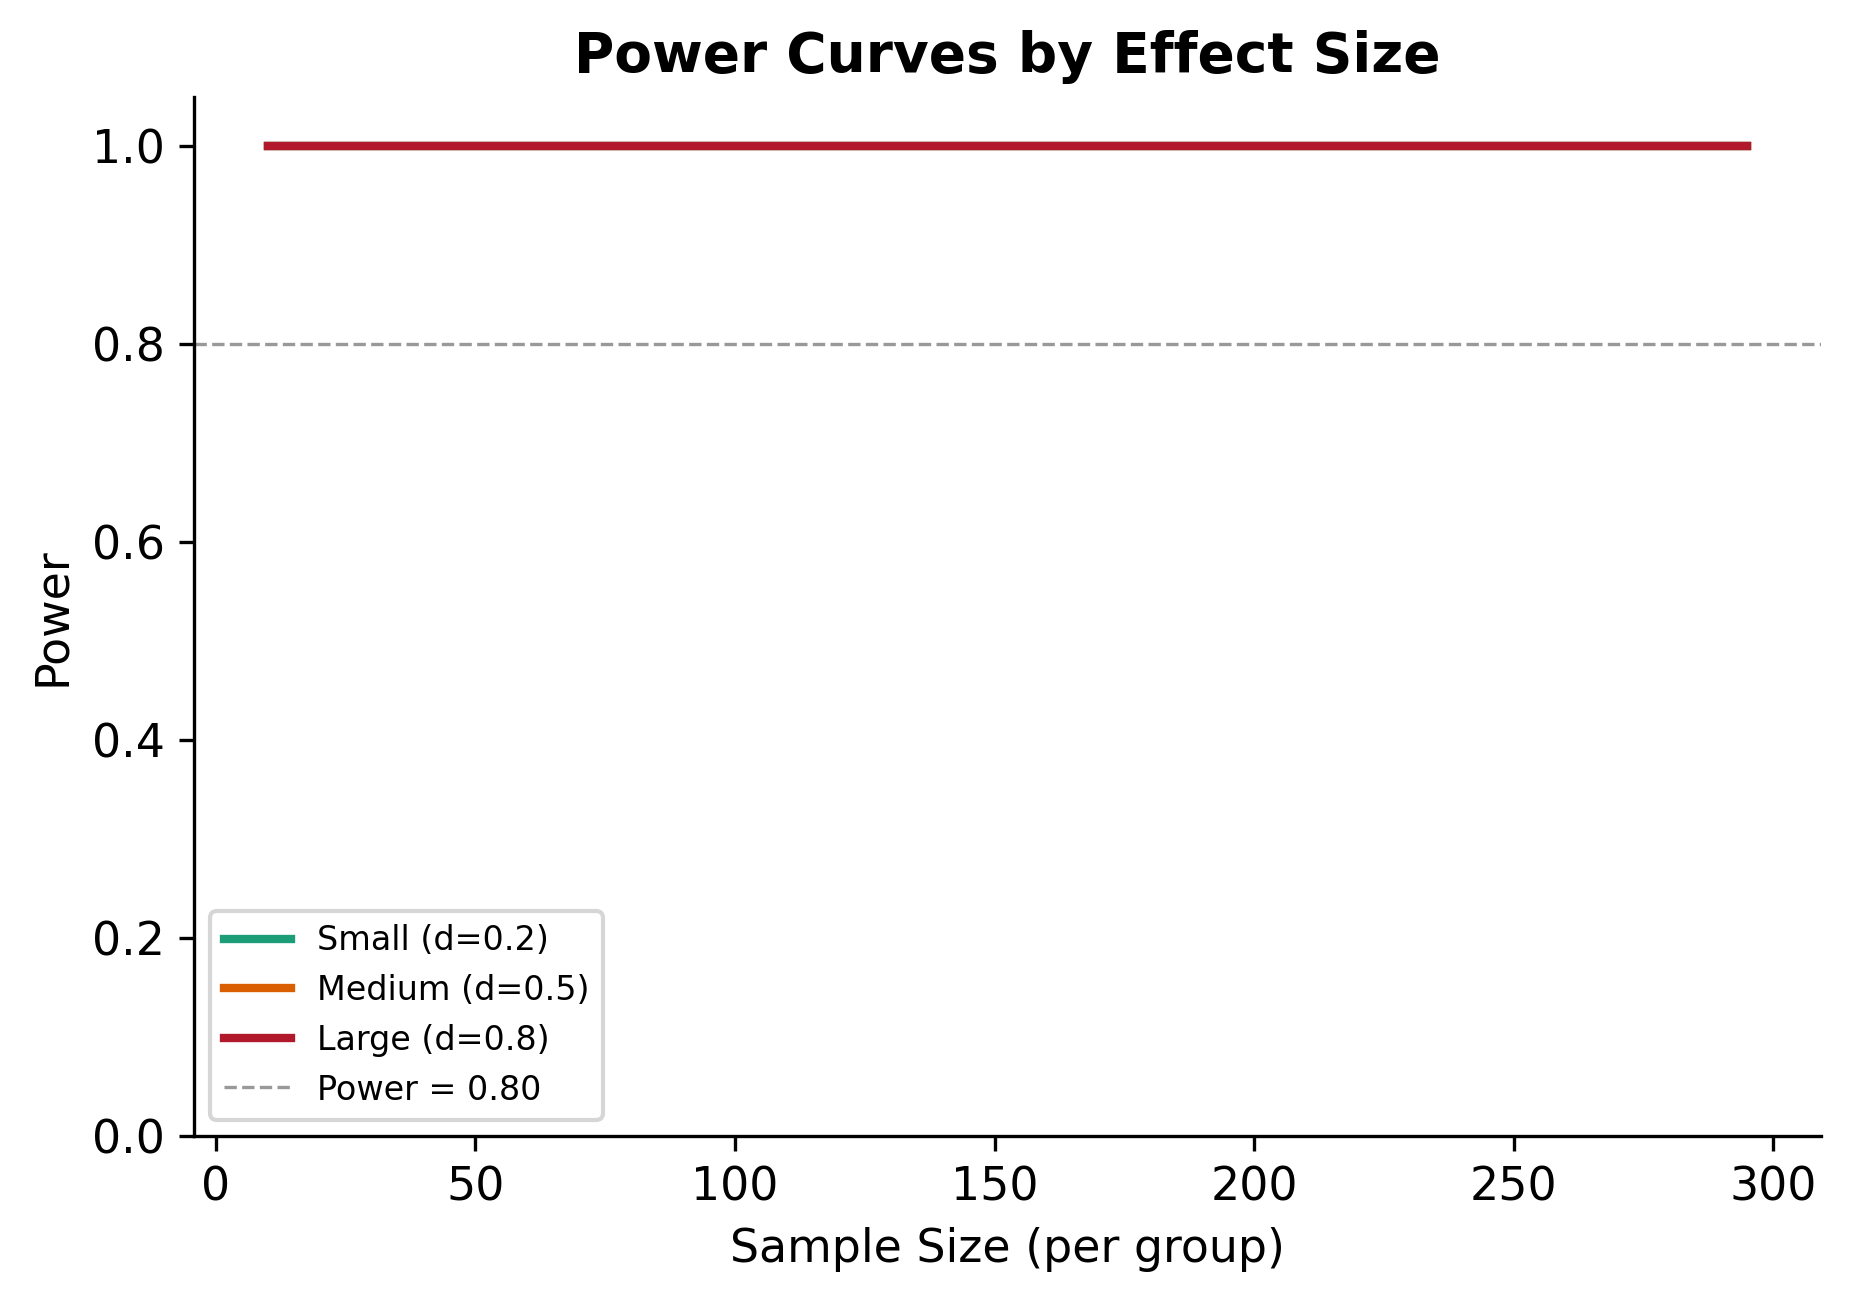
\includegraphics[width=0.72\textwidth]{m2_7_power_curve.png}

\vspace{0.2cm}
\begin{columns}[T]
\begin{column}{0.48\textwidth}
\begin{itemize}
    \item Power = probability of detecting a true effect
    \item $x$-axis = sample size per group
    \item $y$-axis = power (target: 0.80)
    \item Separate curves for small, medium, large effects
    \item Used \textbf{before} data collection for sample planning
\end{itemize}
\end{column}
\begin{column}{0.48\textwidth}
\begin{exampleblock}{Data Insight}
    \scriptsize For a medium effect ($d = 0.5$), you need $\sim$65 per group to reach 80\% power. For a small effect ($d = 0.2$), you need $\sim$400. The power curve makes this trade-off tangible.
\end{exampleblock}
\end{column}
\end{columns}
\end{frame}

% ── 200 ──
\begin{frame}[fragile]{Power Analysis --- Code}\smark{200/300}
\begin{columns}[T]
\begin{column}{0.48\textwidth}
\begin{lstlisting}[style=Rstyle]
library(pwr)

# Required n for d=0.5, 80% power
pwr.t.test(d = 0.5,
  power = 0.80,
  sig.level = 0.05,
  type = "two.sample")
# n = 63.8 per group

# Power curve
ns <- seq(10, 300, 5)
powers <- sapply(ns, function(n)
  pwr.t.test(d=0.5, n=n,
    sig.level=0.05)$power)
plot(ns, powers, type="l")
abline(h=0.8, lty=2)
\end{lstlisting}
\end{column}
\begin{column}{0.48\textwidth}
\begin{lstlisting}[style=Pystyle]
from statsmodels.stats.power \
    import TTestIndPower

analysis = TTestIndPower()

# Required n
n = analysis.solve_power(
    effect_size=0.5, power=0.8,
    alpha=0.05)
# n = 63.8

# Power curve
ns = np.arange(10, 300, 5)
powers = [analysis.power(0.5, n,
    0.05) for n in ns]
ax.plot(ns, powers)
ax.axhline(0.8, linestyle="--")
\end{lstlisting}
\end{column}
\end{columns}
\end{frame}

% ── 201 ──
\begin{frame}{Visualizing Non-Parametric Tests}
\smark{201/300}
\begin{columns}[T]
\begin{column}{0.50\textwidth}
\begin{itemize}
    \item Wilcoxon / Mann--Whitney: compare ranks
    \item Kruskal--Wallis: non-parametric ANOVA
    \item Permutation tests: null from reshuffled labels
    \item Visualize with the \textbf{same} plots as parametric (strip, violin, raincloud) --- the \textbf{test} changes, not the display
\end{itemize}
\end{column}
\begin{column}{0.47\textwidth}
\begin{alertblock}{Pro-Tip}
    \scriptsize In \texttt{ggpubr}: \texttt{stat\_compare\_means(method="wilcox.test")}. In \texttt{statannotations}: \texttt{test="Mann-Whitney"}. The bracket annotation works identically for parametric and non-parametric tests.
\end{alertblock}
\vspace{0.1cm}
\begin{exampleblock}{Data Insight}
    \scriptsize For permutation tests, plot the null distribution of the permuted test statistic as a histogram, then overlay the observed statistic as a vertical line --- exactly like the $t$-test null plot on slide 183.
\end{exampleblock}
\end{column}
\end{columns}
\end{frame}

% ── 202 ──
\begin{frame}[fragile]{Permutation Test Visualization --- Code}\smark{202/300}
\begin{columns}[T]
\begin{column}{0.48\textwidth}
\begin{lstlisting}[style=Rstyle]
library(infer)

# Permutation null distribution
null_dist <- penguins |>
  filter(species %in%
    c("Adelie","Gentoo")) |>
  specify(body_mass_g ~ species) |>
  hypothesize(null="independence")|>
  generate(reps=5000,
    type="permute") |>
  calculate(stat="diff in means")

# Visualize
visualize(null_dist) +
  shade_p_value(
    obs_stat = observed_diff,
    direction = "two-sided")
\end{lstlisting}
\end{column}
\begin{column}{0.48\textwidth}
\begin{lstlisting}[style=Pystyle]
# Manual permutation test
observed = gentoo.mean()-adelie.mean()
combined = np.concatenate(
    [adelie, gentoo])
n_a = len(adelie)

null_diffs = []
for _ in range(5000):
    np.random.shuffle(combined)
    null_diffs.append(
        combined[n_a:].mean() -
        combined[:n_a].mean())

ax.hist(null_diffs, bins=50,
    alpha=0.5, color="#999")
ax.axvline(observed, color="#B2182B",
    linewidth=2, linestyle="--")
p = np.mean(
    np.abs(null_diffs) >= observed)
\end{lstlisting}
\end{column}
\end{columns}
\end{frame}

% ── 203 ──
\begin{frame}{Bayesian Hypothesis Testing: Bayes Factors}
\smark{203/300}
\begin{columns}[T]
\begin{column}{0.50\textwidth}
\begin{itemize}
    \item Bayes Factor ($\text{BF}_{10}$): evidence ratio for $H_1$ vs.\ $H_0$
    \item $\text{BF} > 3$: moderate evidence for $H_1$
    \item $\text{BF} > 10$: strong evidence
    \item $\text{BF} < 1/3$: moderate evidence for $H_0$
    \item $1/3 < \text{BF} < 3$: inconclusive
    \item Unlike $p$: can support the null
\end{itemize}
\end{column}
\begin{column}{0.47\textwidth}
\begin{alertblock}{Pro-Tip}
    \scriptsize R: \texttt{BayesFactor::ttestBF()}. Python: \texttt{pingouin.bayesfactor\_ttest()}. Visualize by plotting the prior and posterior distributions; the BF is the ratio of their heights at the null value.
\end{alertblock}
\vspace{0.1cm}
\begin{exampleblock}{Data Insight}
    \scriptsize The Savage--Dickey density ratio: $\text{BF}_{10} = p(\theta = 0 | \text{prior}) / p(\theta = 0 | \text{posterior})$. If the posterior assigns \emph{less} density at zero than the prior, the data support $H_1$.
\end{exampleblock}
\end{column}
\end{columns}
\end{frame}

% ── 204 ──
\begin{frame}[fragile]{Bayes Factor --- Code}\smark{204/300}
\begin{columns}[T]
\begin{column}{0.48\textwidth}
\begin{lstlisting}[style=Rstyle]
library(BayesFactor)

bf <- ttestBF(adelie_mass,
              gentoo_mass)
bf
# BF10 = 2.4e+54 (overwhelming)

# Visualize prior vs posterior
plot(bf)

# Or bayestestR
library(bayestestR)
describe_posterior(bf)
bf_plot(bf)
\end{lstlisting}
\end{column}
\begin{column}{0.48\textwidth}
\begin{lstlisting}[style=Pystyle]
import pingouin as pg

bf = pg.bayesfactor_ttest(
    stat, nx=len(adelie),
    ny=len(gentoo))
print(f"BF10 = {bf:.2e}")

# Visualize: prior vs posterior
# Prior: Cauchy(0, r=0.707)
# Posterior: from t + df
from scipy.stats import cauchy, t
xs = np.linspace(-5, 5, 300)
ax.plot(xs, cauchy.pdf(xs, 0, 0.707),
    label="Prior", color="#999")
# Posterior requires MCMC or
# analytical approximation
\end{lstlisting}
\end{column}
\end{columns}
\end{frame}

% ── 205 ──
\begin{frame}{ANOVA Visualization: Group Comparisons}
\smark{205/300}
\begin{columns}[T]
\begin{column}{0.50\textwidth}
\begin{itemize}
    \item One-way ANOVA $\to$ ``at least one group differs''
    \item But \textbf{which} groups? $\to$ post-hoc pairwise tests
    \item Visualization: strip/violin + pairwise brackets or estimation contrasts
    \item The plot should show the \textbf{groups}, not the $F$-statistic
\end{itemize}
\end{column}
\begin{column}{0.47\textwidth}
\begin{exampleblock}{Data Insight}
    \scriptsize ANOVA's $F$-test is a global test. It answers ``is there \emph{any} difference?'' but not ``between \emph{which} pairs?'' The visualization should focus on the pairwise contrasts (Module 2.5 style), not the $F$ distribution.
\end{exampleblock}
\vspace{0.1cm}
\begin{alertblock}{Pro-Tip}
    \scriptsize Combine a strip or raincloud plot with \texttt{emmeans} pairwise contrasts rather than adding omnibus $F$-test brackets. The contrasts are what the audience actually needs to interpret.
\end{alertblock}
\end{column}
\end{columns}
\end{frame}

% ── 206 ──
\begin{frame}[fragile]{ANOVA + Post-Hoc --- Code}\smark{206/300}
\begin{columns}[T]
\begin{column}{0.48\textwidth}
\begin{lstlisting}[style=Rstyle]
# ANOVA
model <- aov(body_mass_g ~ species,
             data = penguins)
summary(model)

# Post-hoc: Tukey HSD
TukeyHSD(model)

# Visual: emmeans contrasts
library(emmeans)
emm <- emmeans(model, ~ species)
plot(pairs(emm)) +
  geom_vline(xintercept=0,
    linetype="dashed") +
  theme_minimal()
\end{lstlisting}
\end{column}
\begin{column}{0.48\textwidth}
\begin{lstlisting}[style=Pystyle]
from scipy.stats import f_oneway

F, p = f_oneway(
    adelie, chinstrap, gentoo)

# Post-hoc: Tukey HSD
from statsmodels.stats.multicomp \
    import pairwise_tukeyhsd
tukey = pairwise_tukeyhsd(
    penguins["body_mass_g"],
    penguins["species"])
tukey.plot_simultaneous()

# pingouin
pg.anova(data=penguins,
    dv="body_mass_g",
    between="species")
pg.pairwise_tukey(data=penguins,
    dv="body_mass_g",
    between="species")
\end{lstlisting}
\end{column}
\end{columns}
\end{frame}

% ── 207 ──
\begin{frame}{Reporting Guidelines: What to Show}
\smark{207/300}
\centering\small
\begin{tabular}{@{}ll@{}}
    \toprule
    \textbf{Show} & \textbf{Why} \\
    \midrule
    Raw data (strip / jitter / raincloud)  & Distribution shape, $n$, outliers \\
    Effect size $\pm$ CI                    & Practical magnitude + precision \\
    Bootstrap or model-based CI             & Non-parametric robustness \\
    Estimation plot (if comparing 2 groups) & Directly answers ``how big is the difference?'' \\
    \midrule
    \textbf{Optional (add if required)} & \\
    \midrule
    $p$-value (in caption, not on plot)     & Satisfies reviewers \\
    Significance brackets                   & If journal demands them \\
    Bayes Factor                            & Evidence for or against $H_0$ \\
    \bottomrule
\end{tabular}

\vspace{0.3cm}
\begin{alertblock}{Pro-Tip}
    \scriptsize Lead with \textbf{data + effect size + CI}. Report $p$-values in the text or caption if needed. Never let the star bracket be the primary visual takeaway.
\end{alertblock}
\end{frame}

% ── 208 ──
\begin{frame}{Common Mistakes in Test Visualization}
\smark{208/300}
\centering\small
\begin{tabular}{@{}ll@{}}
    \toprule
    \textbf{Mistake} & \textbf{Fix} \\
    \midrule
    Bar chart + stars only                     & Strip/raincloud + effect size CI \\
    $p$-value without effect size              & Report $d$ or $\Delta$ with CI \\
    Overlapping CIs $\to$ ``not significant''  & Formal test on the \emph{difference} \\
    No multiple-testing correction             & FDR or Bonferroni \\
    Stars on bar chart of $n = 5$              & Show all 5 points (no summary geom) \\
    Volcano with raw $p$                       & Use FDR-adjusted $p$ \\
    Underpowered study reported as ``ns''      & Report power or CI width \\
    \bottomrule
\end{tabular}
\end{frame}

% ── 209 ──
\begin{frame}{Hypothesis Testing Decision Guide}
\smark{209/300}
\centering\small
\begin{tabular}{@{}lll@{}}
    \toprule
    \textbf{Question} & \textbf{Visual} & \textbf{Tool} \\
    \midrule
    2 groups, continuous     & Estimation plot      & \texttt{dabestr} \\
    3+ groups, continuous    & Strip + pairwise CI  & \texttt{emmeans} contrasts \\
    Effect magnitude         & Cohen's $d$ overlap  & \texttt{effectsize} / \texttt{pingouin} \\
    Genomic / high-dim       & Volcano plot         & \texttt{EnhancedVolcano} \\
    Sample planning          & Power curve          & \texttt{pwr} / \texttt{TTestIndPower} \\
    Bayesian evidence        & Prior vs.\ posterior & \texttt{bayesplot} / \texttt{arviz} \\
    Permutation null         & Null histogram       & \texttt{infer} / manual \\
    \bottomrule
\end{tabular}
\end{frame}

% ── 210 ──
\begin{frame}{Module 2.7 --- Key Takeaways}\smark{210/300}
\begin{enumerate}
    \item \textbf{$p$-value = tail area}, not a binary switch. Visualize it.
    \item \textbf{Effect size + CI} is more informative than $p$ alone.
    \item \textbf{Estimation plots} (dabestr) replace bar + star brackets.
    \item \textbf{Volcano plots} handle thousands of simultaneous tests.
    \item \textbf{Power curves} should be plotted \textbf{before} collecting data.
    \item \textbf{Lead with data and effect size.} Report $p$ in the caption.
\end{enumerate}
\end{frame}

% ── 211 ──
\begin{frame}{}\smark{211/300}
\centering\vspace{1.5cm}
{\Large\textbf{Module 2.7 Complete}}\\[0.5cm]
You can now visualize hypothesis tests, $p$-values, effect sizes, estimation statistics, volcano plots, and power analyses --- and know when to let go of the star bracket.\\[0.5cm]
\textbf{Next:} Module 2.8 --- Classification Diagnostics: ROC, Confusion, Calibration.
\end{frame}

% 
% ═══════════════════════════════════════════════════════
%  MODULE 2.8 — Classification Diagnostics: ROC, Confusion, Calibration
% ═══════════════════════════════════════════════════════
\section{Module 2.8 --- Classification Diagnostics}

% ── 212 ──
\begin{frame}{Module 2.8 --- Roadmap}\smark{212/300}
\begin{enumerate}
    \item Confusion matrix heatmap
    \item Score distributions by true class
    \item ROC curve: TPR vs.\ FPR and AUC
    \item Precision-Recall curve for imbalanced data
    \item Calibration plots (reliability diagrams)
    \item Threshold tuning: metrics vs.\ cut-off
    \item Gain and lift charts
    \item Multi-class extensions
\end{enumerate}
\end{frame}

% ── 213 ──
\begin{frame}{Confusion Matrix Heatmap}\smark{213/300}
\centering
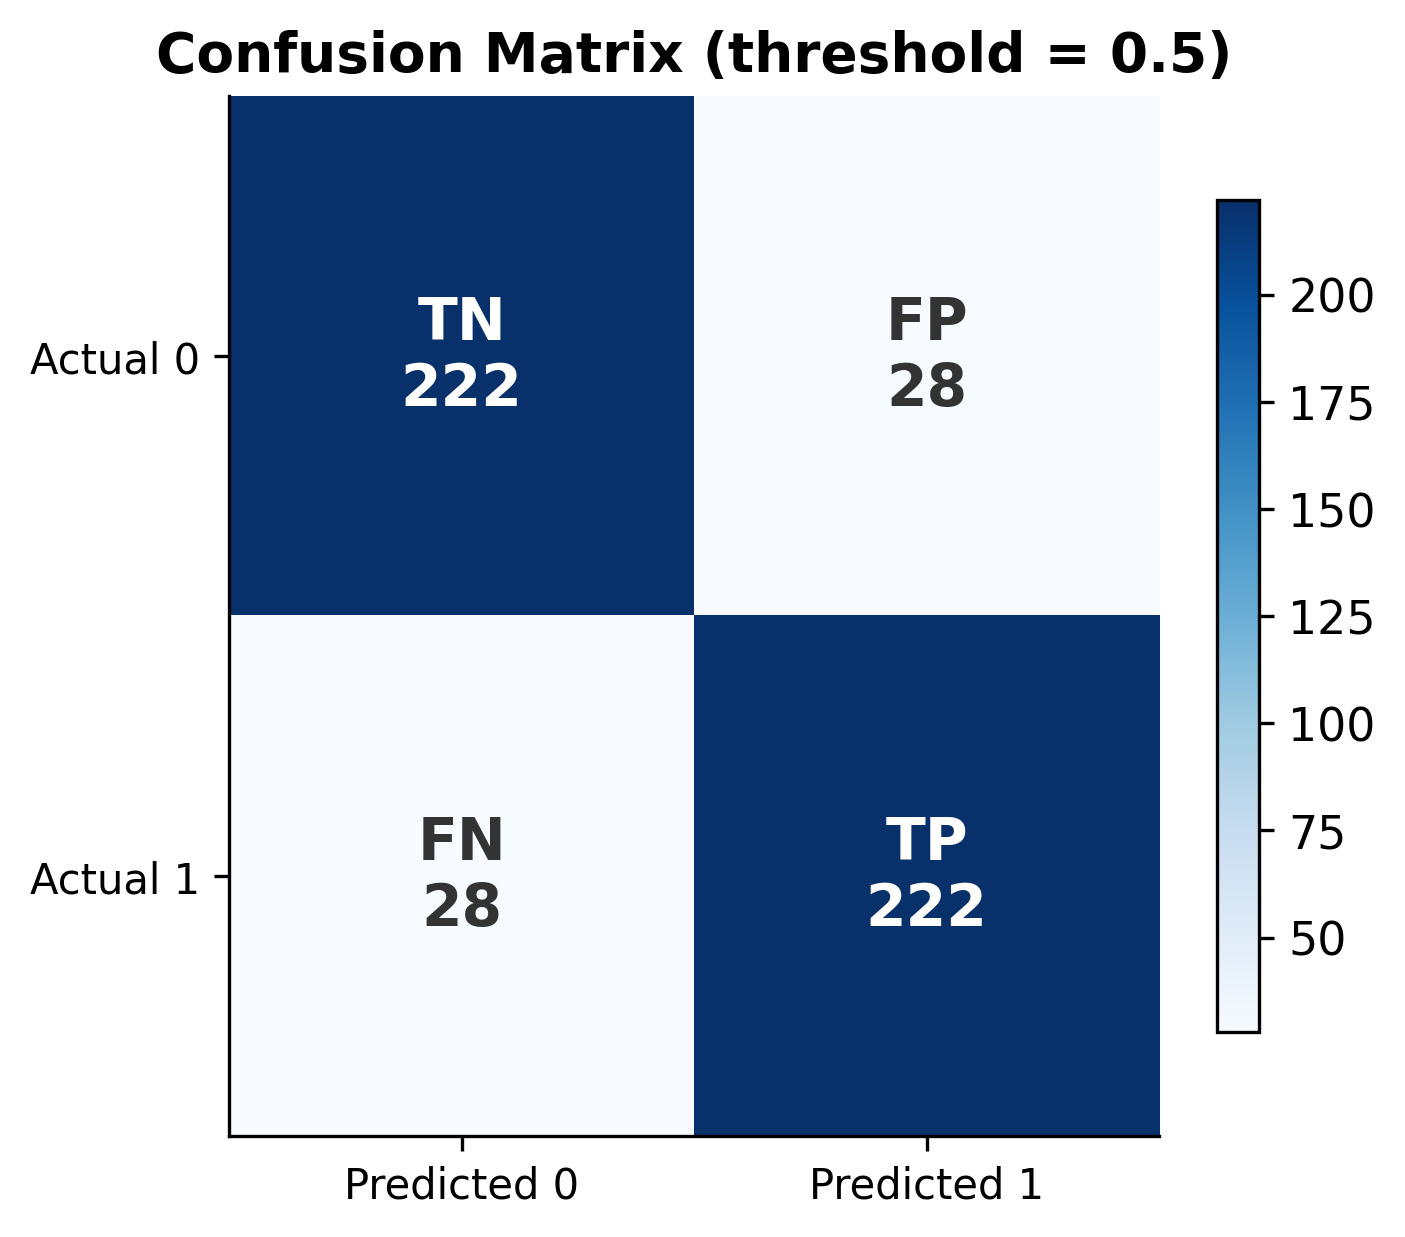
\includegraphics[width=0.52\textwidth]{m2_8_confusion_matrix.png}
\vspace{0.2cm}
\begin{columns}[T]
\begin{column}{0.48\textwidth}
\centering\small
\begin{tabular}{@{}lll@{}}
    \toprule
     & \textbf{Pred 0} & \textbf{Pred 1} \\
    \midrule
    \textbf{True 0} & TN & FP (Type I) \\
    \textbf{True 1} & FN (Type II) & TP \\
    \bottomrule
\end{tabular}
\end{column}
\begin{column}{0.48\textwidth}
\begin{exampleblock}{Data Insight}
    \scriptsize The diagonal = correct; off-diagonal = errors. Color intensity maps to count. The matrix reveals whether errors bias toward false positives or false negatives.
\end{exampleblock}
\end{column}
\end{columns}
\end{frame}

% ── 214 ──
\begin{frame}[fragile]{Confusion Matrix --- \Rlang}\smark{214/300}
\begin{columns}[T]
\begin{column}{0.55\textwidth}
\begin{lstlisting}[style=Rstyle]
library(yardstick)
cm <- conf_mat(df, truth, estimate)
autoplot(cm, type = "heatmap")

# caret alternative
library(caret)
cm <- confusionMatrix(
  factor(pred), factor(actual))

# cvms for styled output
library(cvms)
plot_confusion_matrix(
  as_tibble(cm$table),
  target_col = "Reference",
  prediction_col = "Prediction",
  counts_col = "n")
\end{lstlisting}
\end{column}
\begin{column}{0.42\textwidth}
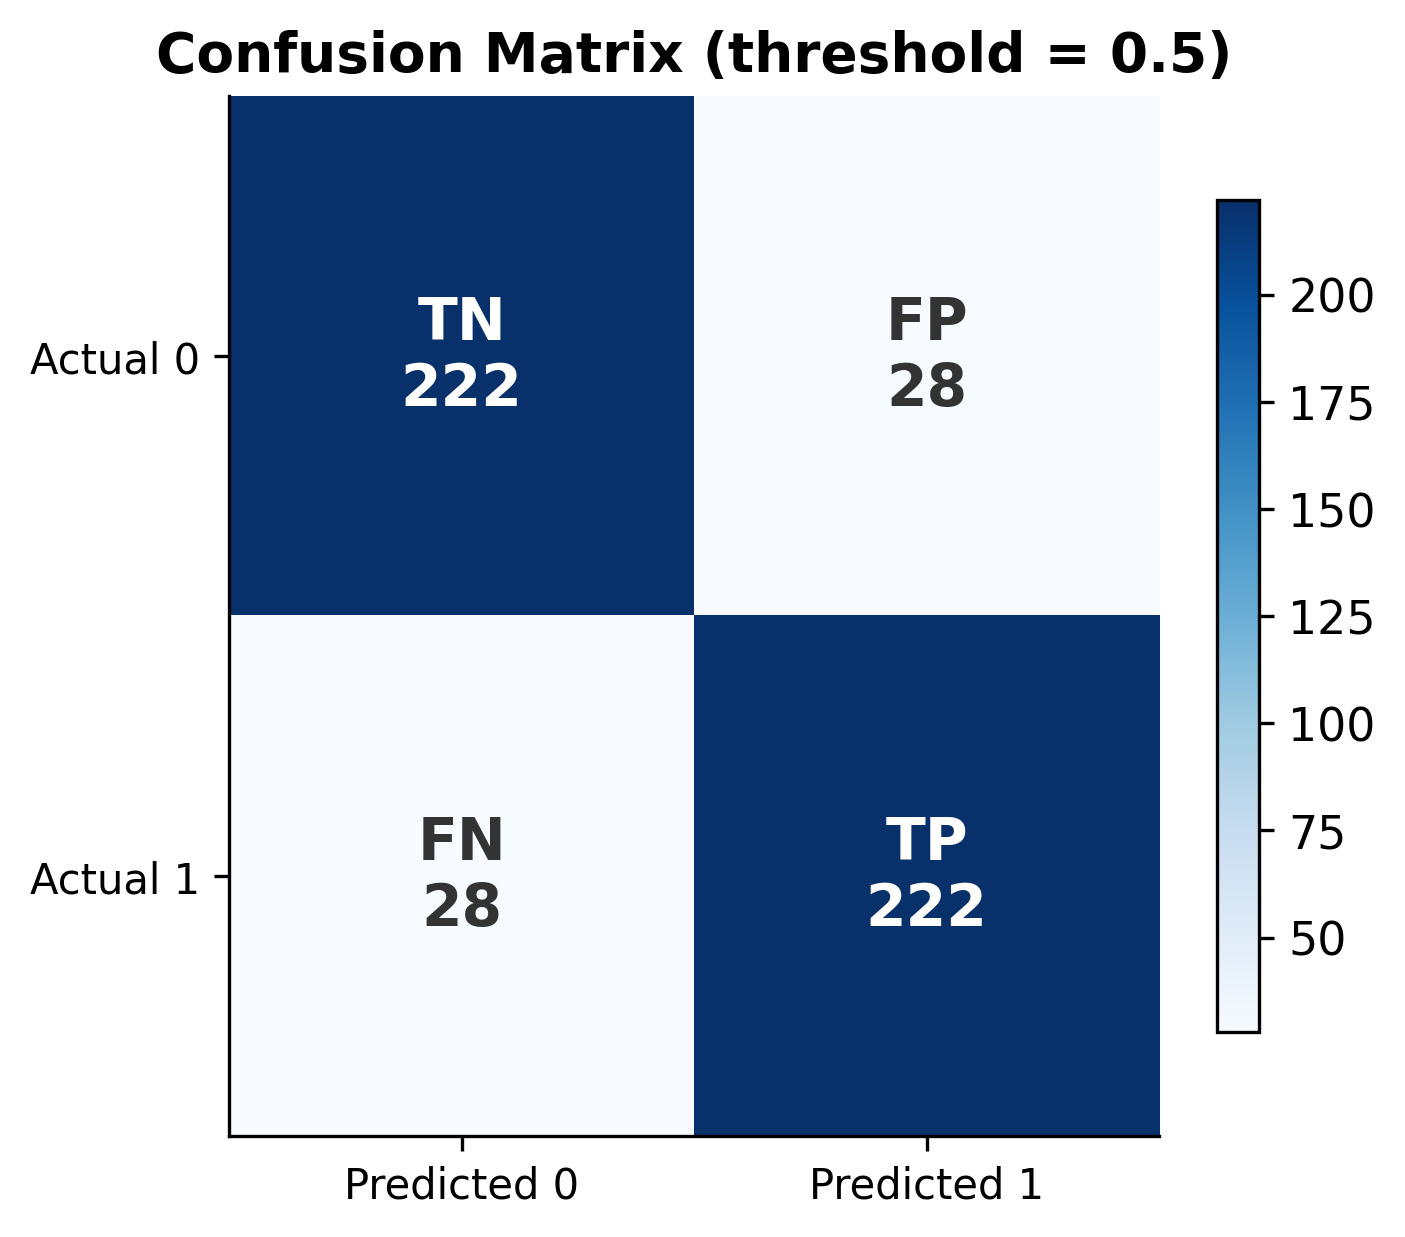
\includegraphics[width=\textwidth]{m2_8_confusion_matrix.png}
\begin{alertblock}{Pro-Tip}
    \scriptsize \texttt{yardstick::autoplot(type="heatmap")} produces ggplot2-based output. \texttt{type="mosaic"} shows proportions instead of counts.
\end{alertblock}
\end{column}
\end{columns}
\end{frame}

% ── 215 ──
\begin{frame}[fragile]{Confusion Matrix --- \Python}\smark{215/300}
\begin{columns}[T]
\begin{column}{0.55\textwidth}
\begin{lstlisting}[style=Pystyle]
from sklearn.metrics import (
    confusion_matrix,
    ConfusionMatrixDisplay)

cm = confusion_matrix(y_true, y_pred)
ConfusionMatrixDisplay.from_predictions(
    y_true, y_pred,
    cmap="Blues",
    display_labels=["Neg","Pos"])

# seaborn heatmap
sns.heatmap(cm, annot=True,
    fmt="d", cmap="Blues",
    xticklabels=["Neg","Pos"],
    yticklabels=["Neg","Pos"])
plt.xlabel("Predicted")
plt.ylabel("Actual")
\end{lstlisting}
\end{column}
\begin{column}{0.42\textwidth}
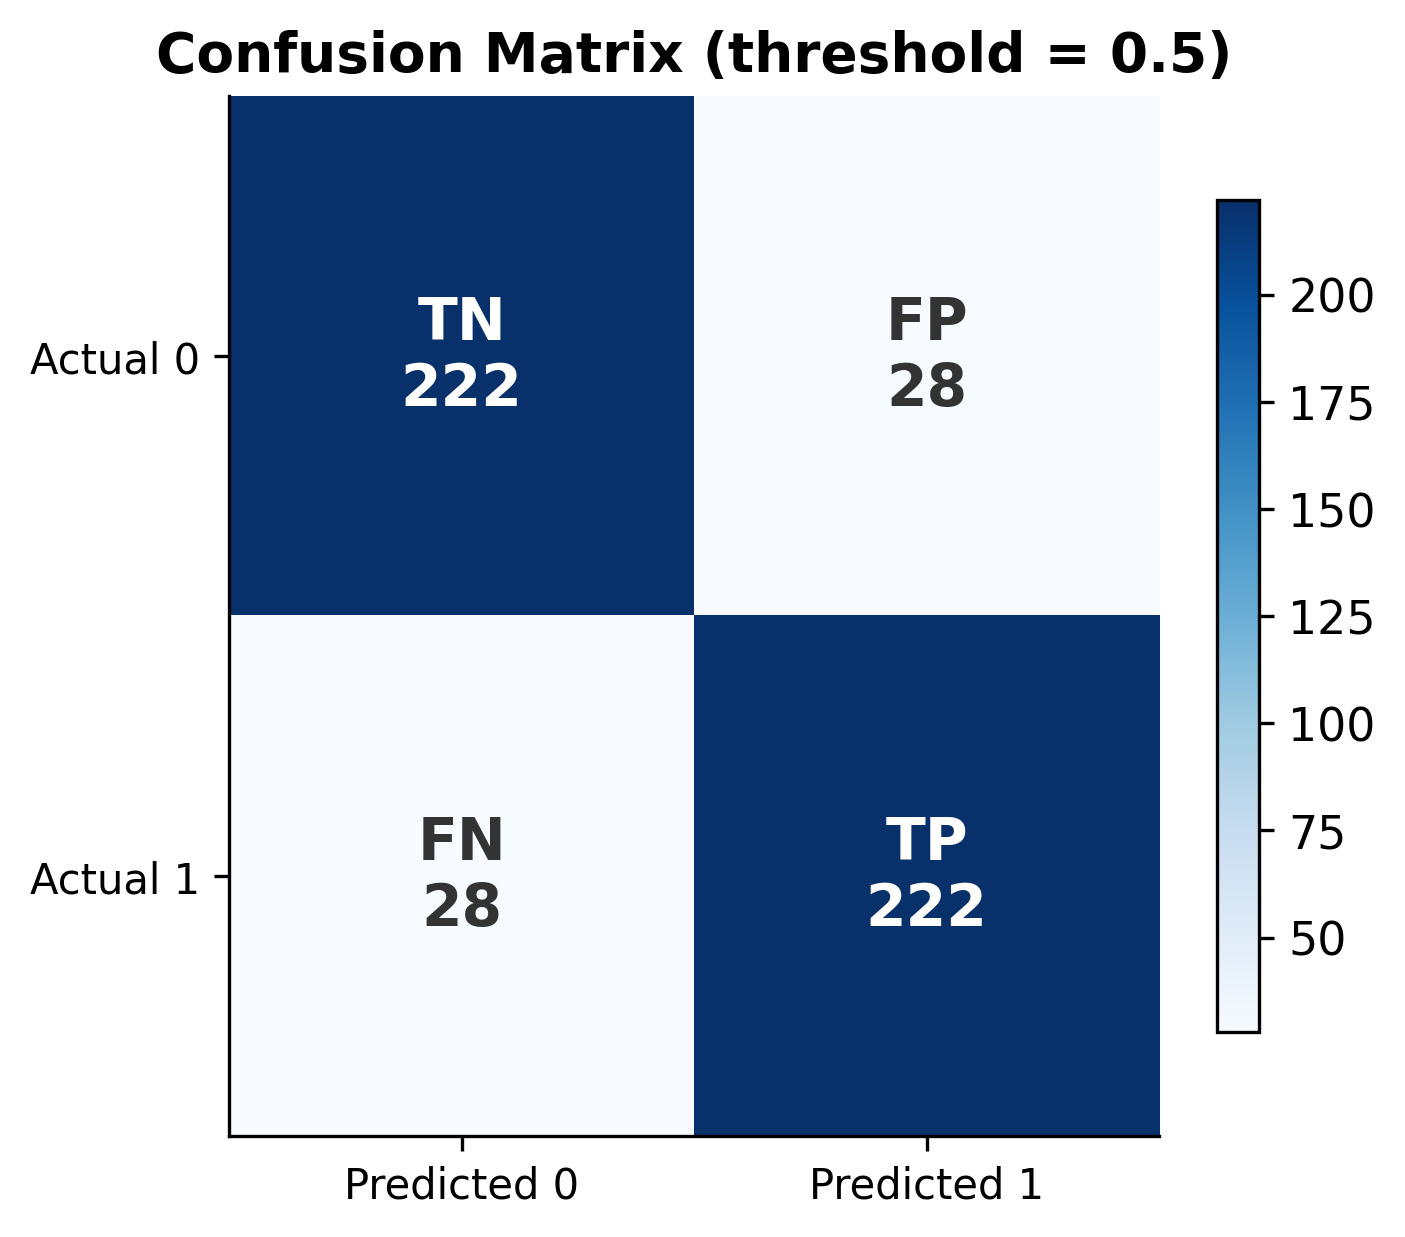
\includegraphics[width=\textwidth]{m2_8_confusion_matrix.png}
\begin{exampleblock}{Data Insight}
    \scriptsize \texttt{ConfusionMatrixDisplay} is scikit-learn's built-in. For custom styling, extract \texttt{confusion\_matrix()} and plot with seaborn.
\end{exampleblock}
\end{column}
\end{columns}
\end{frame}

% ── 216 ──
\begin{frame}{Score Distributions by True Class}\smark{216/300}
\centering
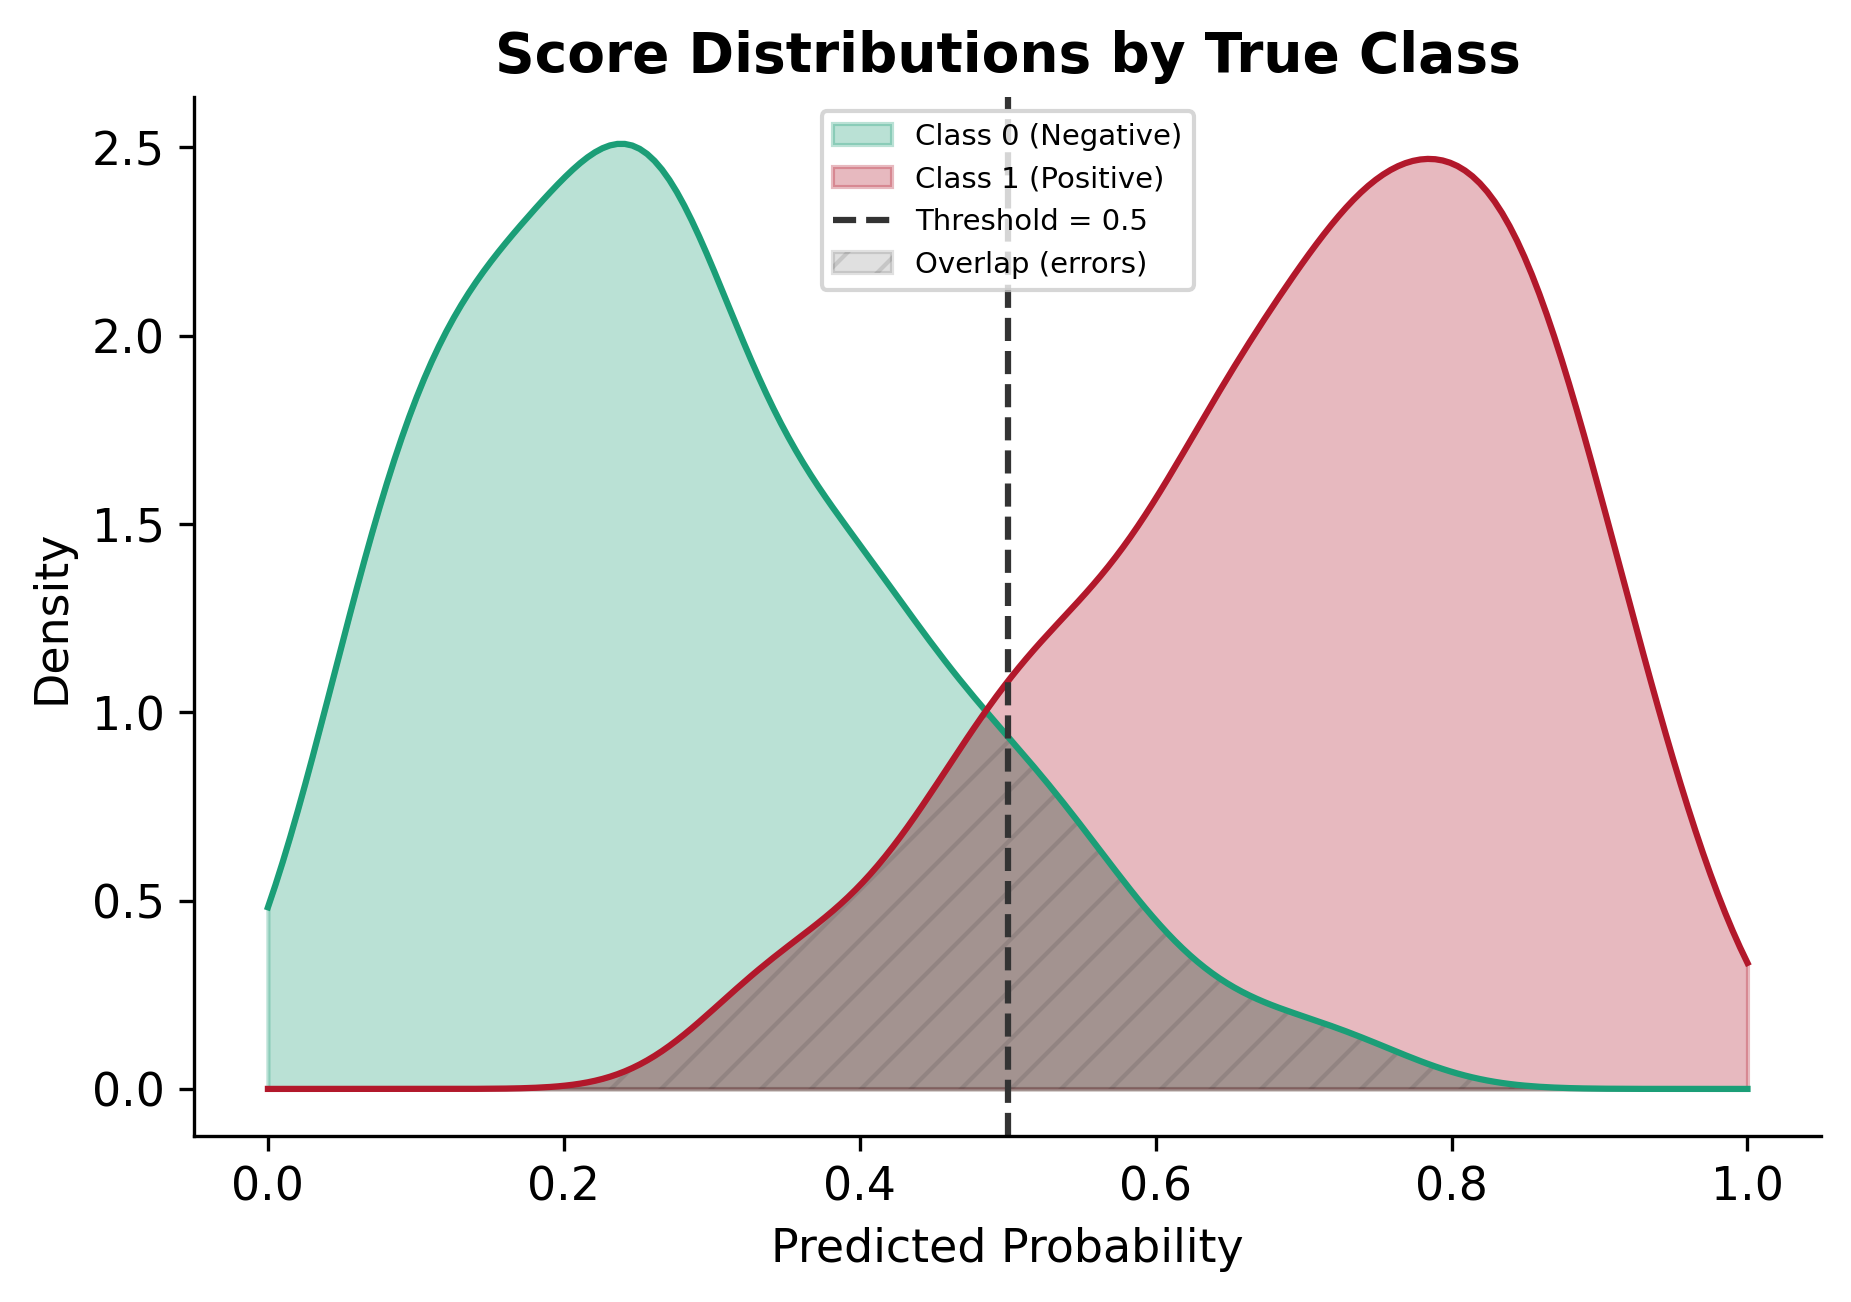
\includegraphics[width=0.72\textwidth]{m2_8_score_dist.png}
\vspace{0.2cm}
\begin{columns}[T]
\begin{column}{0.48\textwidth}
\begin{itemize}
    \item KDE of predicted probabilities, split by true label
    \item \textbf{Separation} = model discriminability
    \item \textbf{Overlap zone} (hatched) = errors regardless of threshold
    \item The threshold trades FP for FN
\end{itemize}
\end{column}
\begin{column}{0.48\textwidth}
\begin{exampleblock}{Data Insight}
    \scriptsize A perfect model shows zero overlap. The overlap region is the irreducible error for any threshold. Moving the threshold left trades more FP for fewer FN.
\end{exampleblock}
\end{column}
\end{columns}
\end{frame}

% ── 217 ──
\begin{frame}[fragile]{Score Distributions --- Code}\smark{217/300}
\begin{columns}[T]
\begin{column}{0.48\textwidth}
\begin{lstlisting}[style=Rstyle]
df <- tibble(score=scores,
  class=factor(y_true))
ggplot(df, aes(score,
    fill=class, color=class)) +
  geom_density(alpha=0.3) +
  geom_vline(xintercept=0.5,
    linetype="dashed") +
  scale_fill_manual(
    values=c("#1B9E77","#B2182B"))+
  theme_minimal()
\end{lstlisting}
\end{column}
\begin{column}{0.48\textwidth}
\begin{lstlisting}[style=Pystyle]
for label, c, name in [
    (0, "#1B9E77", "Negative"),
    (1, "#B2182B", "Positive")]:
    subset = scores[y_true==label]
    sns.kdeplot(subset, fill=True,
        alpha=0.3, color=c,
        label=name, ax=ax)
ax.axvline(0.5, linestyle="--",
    color="#333")
\end{lstlisting}
\begin{alertblock}{Pro-Tip}
    \scriptsize Plot score distributions \textbf{before} choosing a threshold. The visual tells you how much error any threshold will incur.
\end{alertblock}
\end{column}
\end{columns}
\end{frame}

% ── 218 ──
\begin{frame}{ROC Curve: TPR vs.\ FPR}\smark{218/300}
\centering
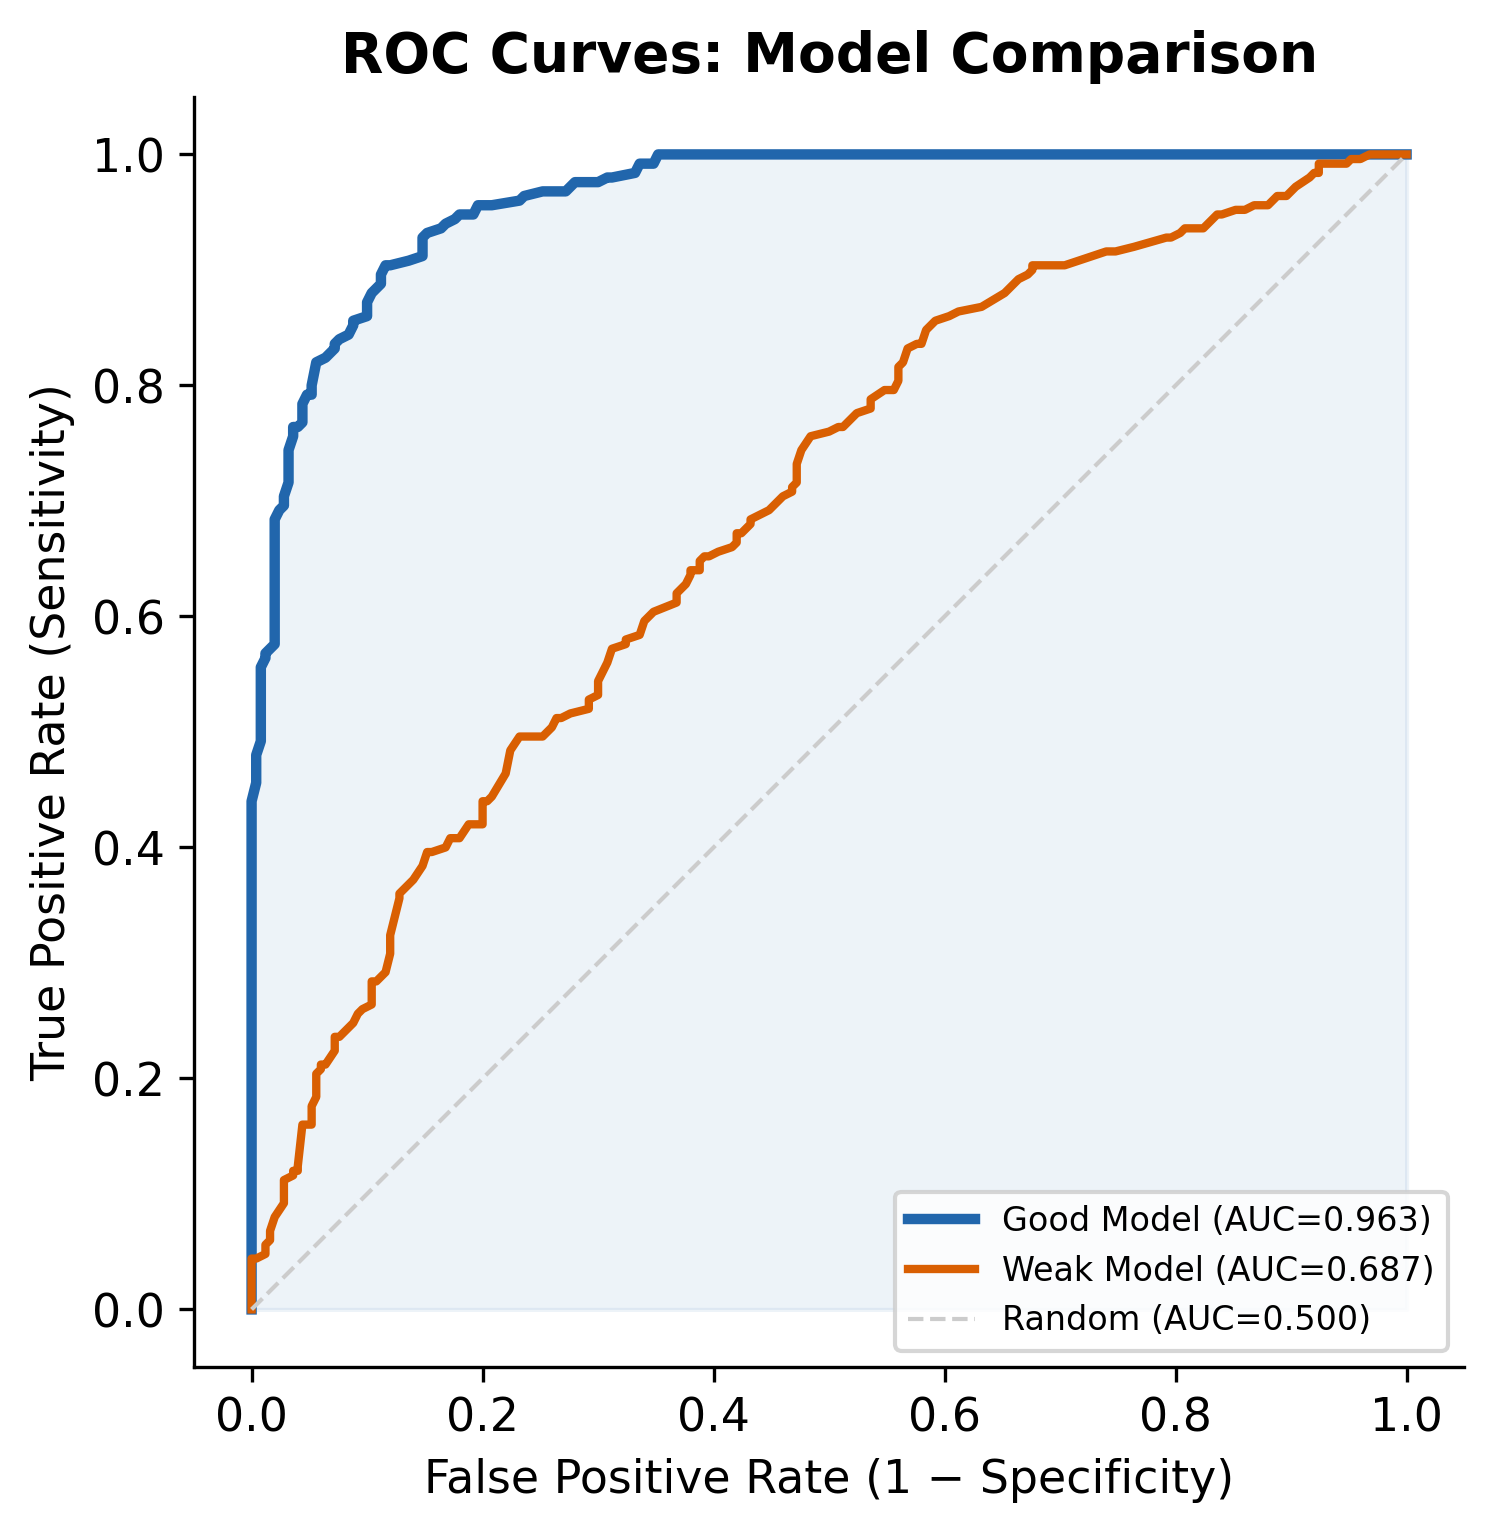
\includegraphics[width=0.58\textwidth]{m2_8_roc_curve.png}
\vspace{0.2cm}
\begin{columns}[T]
\begin{column}{0.48\textwidth}
\begin{itemize}
    \item $x$: FPR = FP/(FP+TN)
    \item $y$: TPR = TP/(TP+FN)
    \item Each point = one threshold
    \item AUC: 0.5 = random, 1.0 = perfect
    \item Threshold-independent discrimination summary
\end{itemize}
\end{column}
\begin{column}{0.48\textwidth}
\begin{exampleblock}{Data Insight}
    \scriptsize Good model (AUC=0.963) hugs upper-left. Weak model (AUC=0.687) is closer to the diagonal. AUC measures how well the model ranks positives above negatives.
\end{exampleblock}
\end{column}
\end{columns}
\end{frame}

% ── 219 ──
\begin{frame}[fragile]{ROC Curve --- \Rlang}\smark{219/300}
\begin{columns}[T]
\begin{column}{0.55\textwidth}
\begin{lstlisting}[style=Rstyle]
library(pROC)
roc_obj <- roc(y_true, scores)
auc(roc_obj)  # 0.963

# ggplot2 version
ggroc(roc_obj) +
  geom_abline(slope=1, intercept=1,
    linetype="dashed", color="#CCC")+
  annotate("text", x=0.3, y=0.3,
    label=paste0("AUC = ",
      round(auc(roc_obj), 3))) +
  theme_minimal()

# Multiple models
ggroc(list(good=roc_g, weak=roc_w))
\end{lstlisting}
\end{column}
\begin{column}{0.42\textwidth}
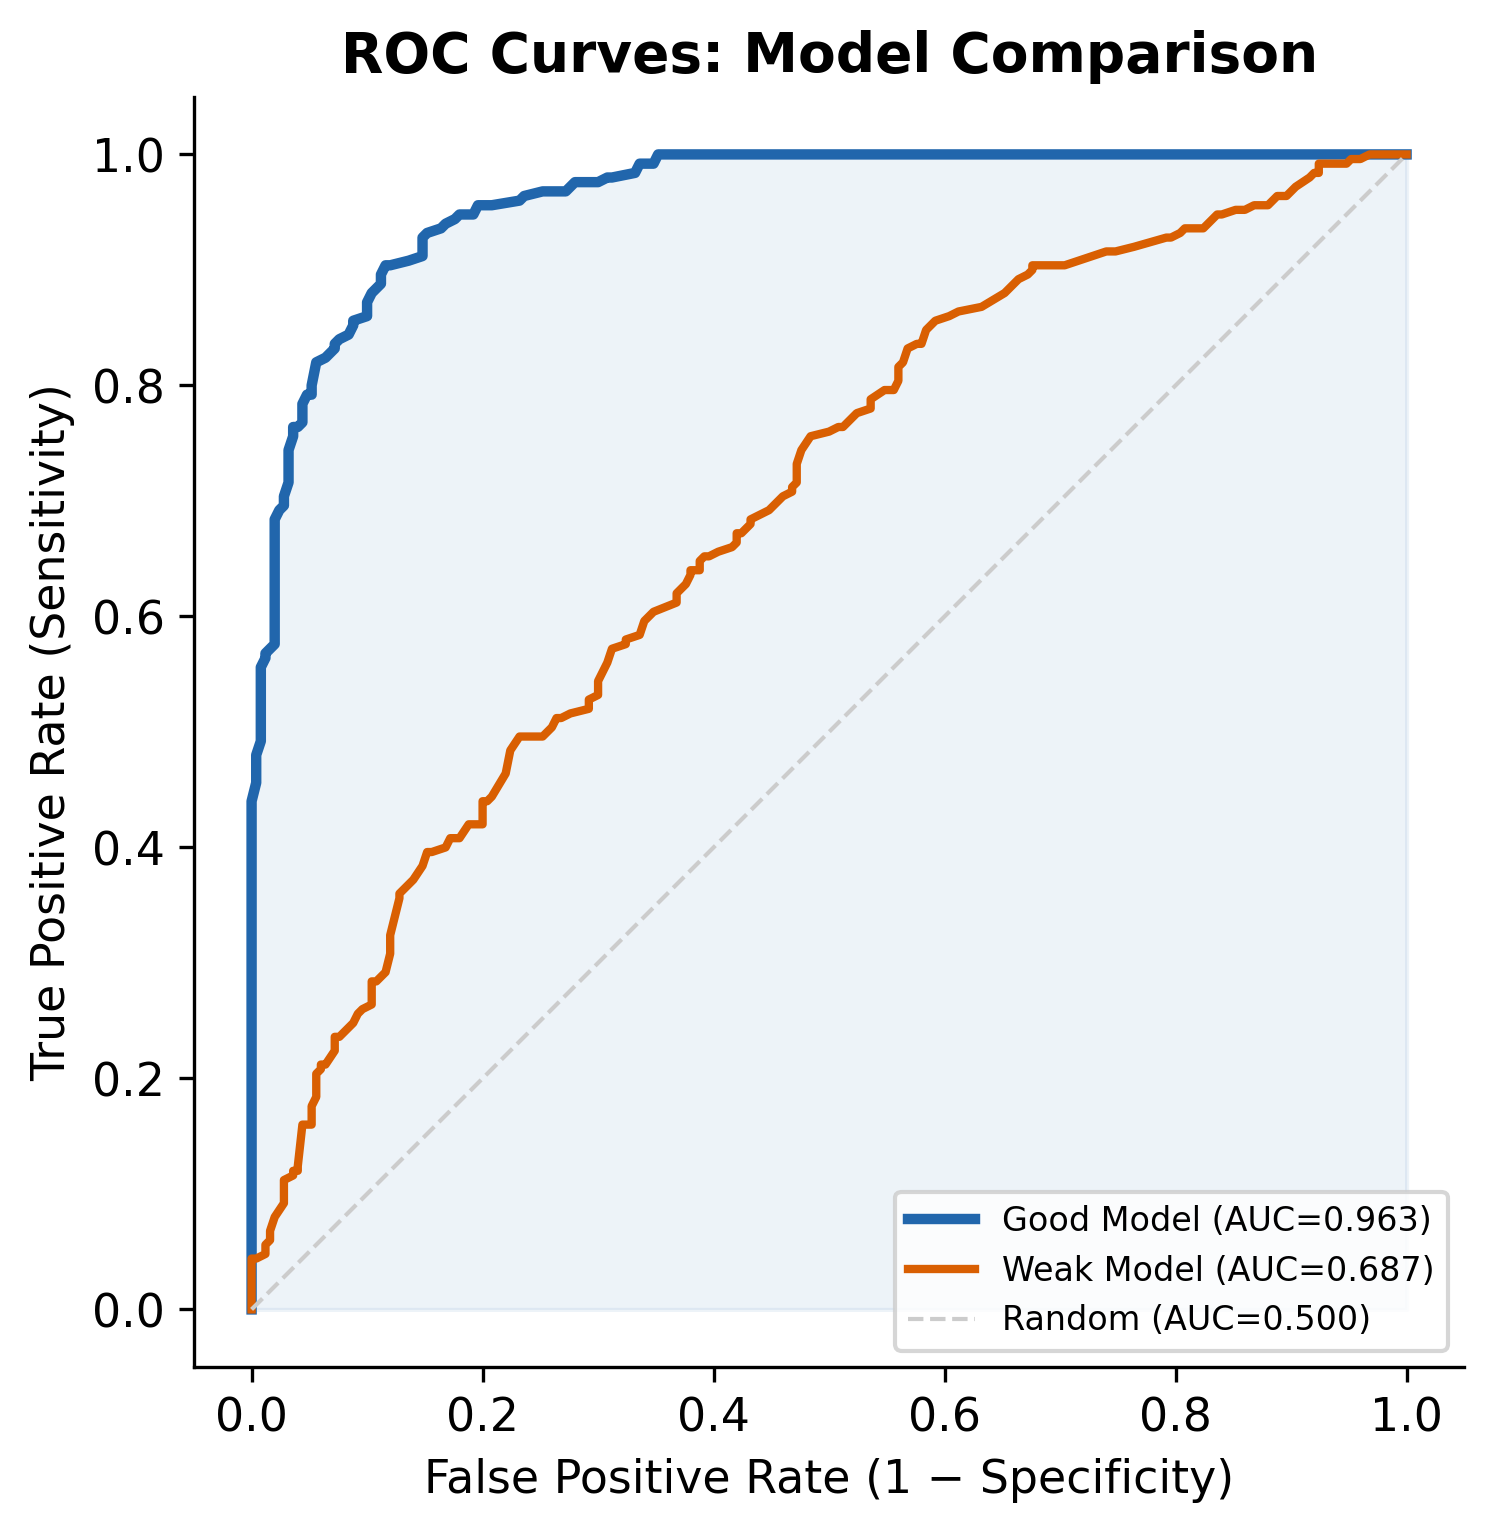
\includegraphics[width=\textwidth]{m2_8_roc_curve.png}
\begin{alertblock}{Pro-Tip}
    \scriptsize \texttt{pROC::ggroc()} reverses x-axis by default. Add \texttt{legacy.axes=TRUE} for standard FPR on $x$.
\end{alertblock}
\end{column}
\end{columns}
\end{frame}

% ── 220 ──
\begin{frame}[fragile]{ROC Curve --- \Python}\smark{220/300}
\begin{columns}[T]
\begin{column}{0.55\textwidth}
\begin{lstlisting}[style=Pystyle]
from sklearn.metrics import (
    roc_curve, roc_auc_score,
    RocCurveDisplay)

RocCurveDisplay.from_predictions(
    y_true, scores, name="Model")

# Manual
fpr, tpr, thresholds = roc_curve(
    y_true, scores)
auc_val = roc_auc_score(y_true,scores)
ax.plot(fpr, tpr, color="#2166AC",
    linewidth=2,
    label=f"AUC = {auc_val:.3f}")
ax.plot([0,1],[0,1],"--",color="#CCC")
\end{lstlisting}
\end{column}
\begin{column}{0.42\textwidth}
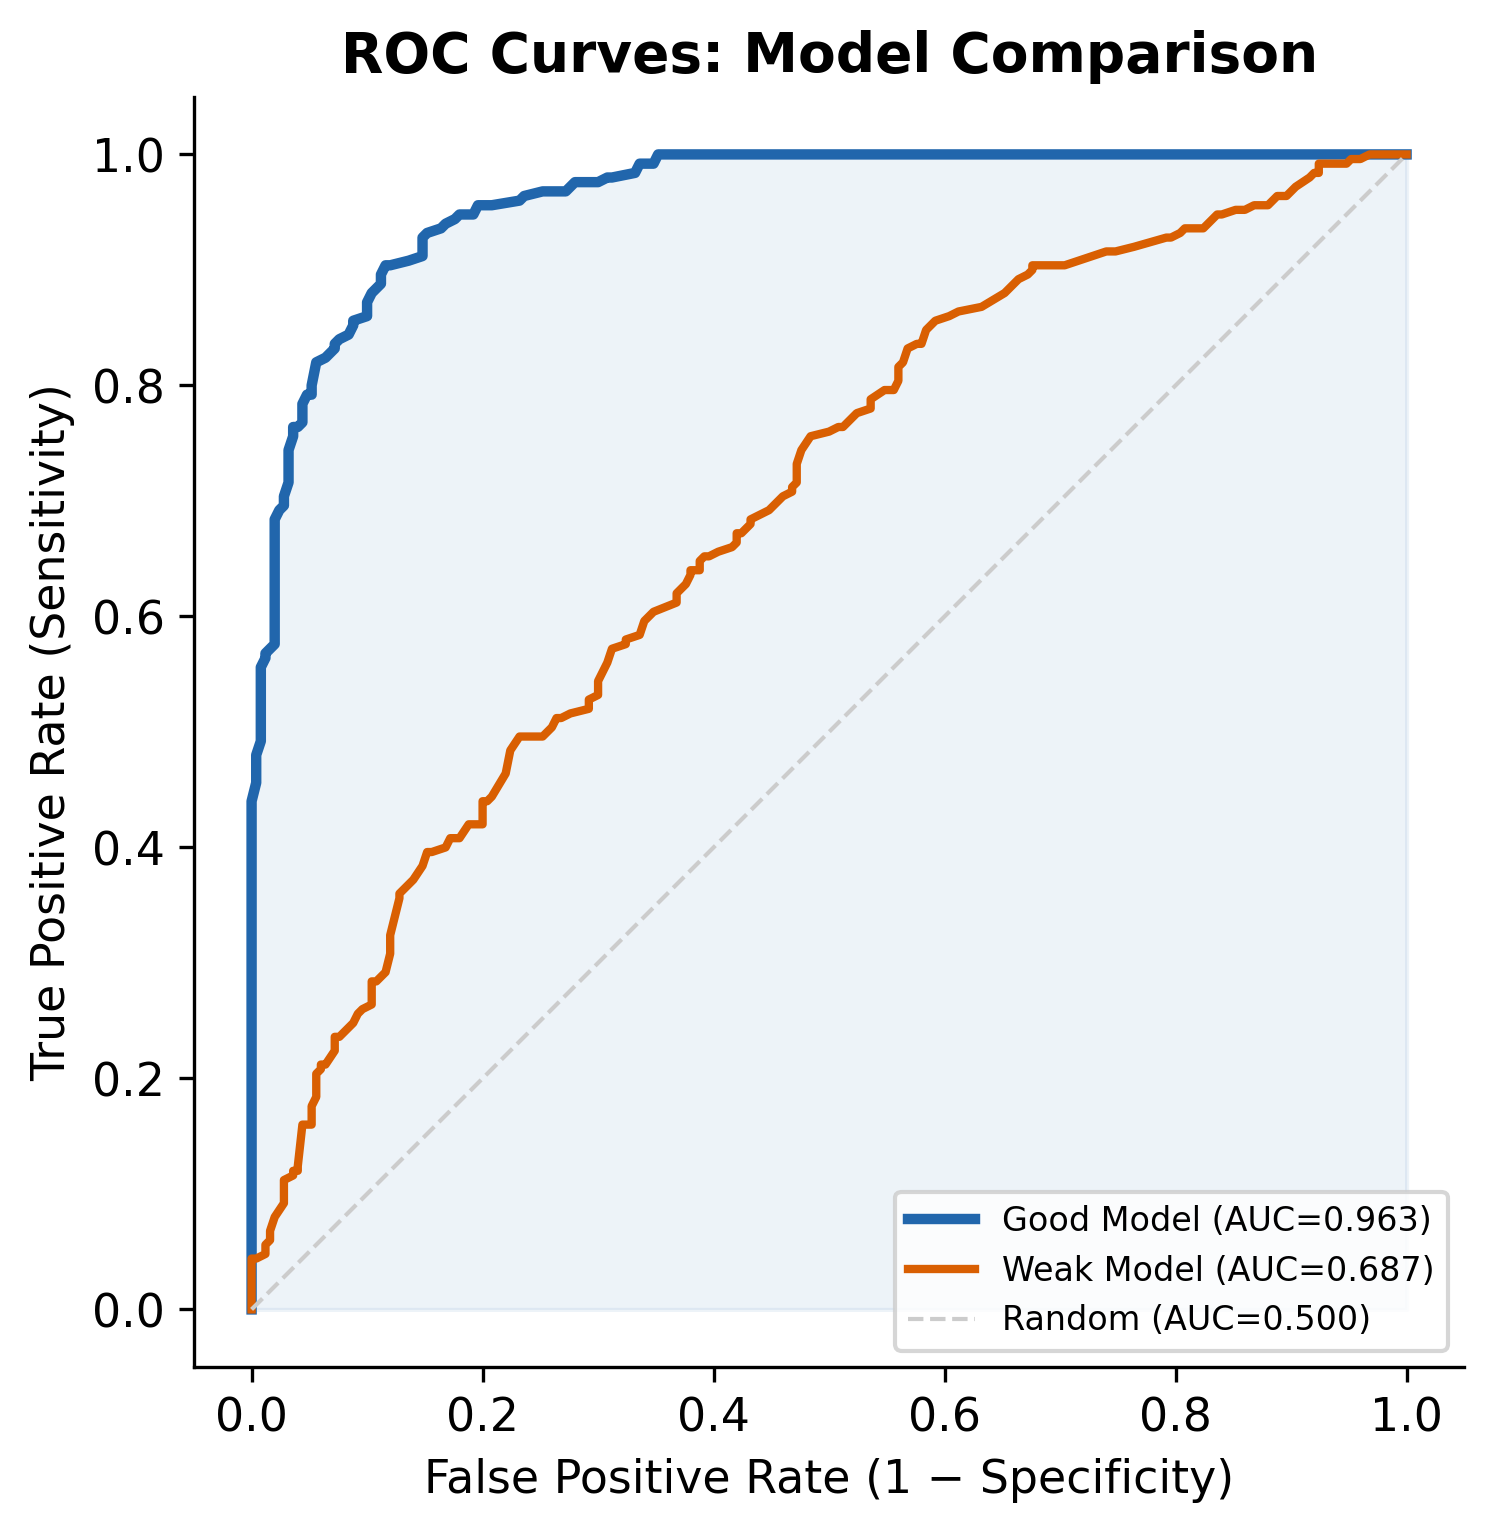
\includegraphics[width=\textwidth]{m2_8_roc_curve.png}
\begin{exampleblock}{Data Insight}
    \scriptsize \texttt{RocCurveDisplay.from\_predictions()} is scikit-learn's one-liner. Call multiple times on the same axis for model comparison.
\end{exampleblock}
\end{column}
\end{columns}
\end{frame}

% ── 221 ──
\begin{frame}{Precision-Recall Curve}\smark{221/300}
\centering
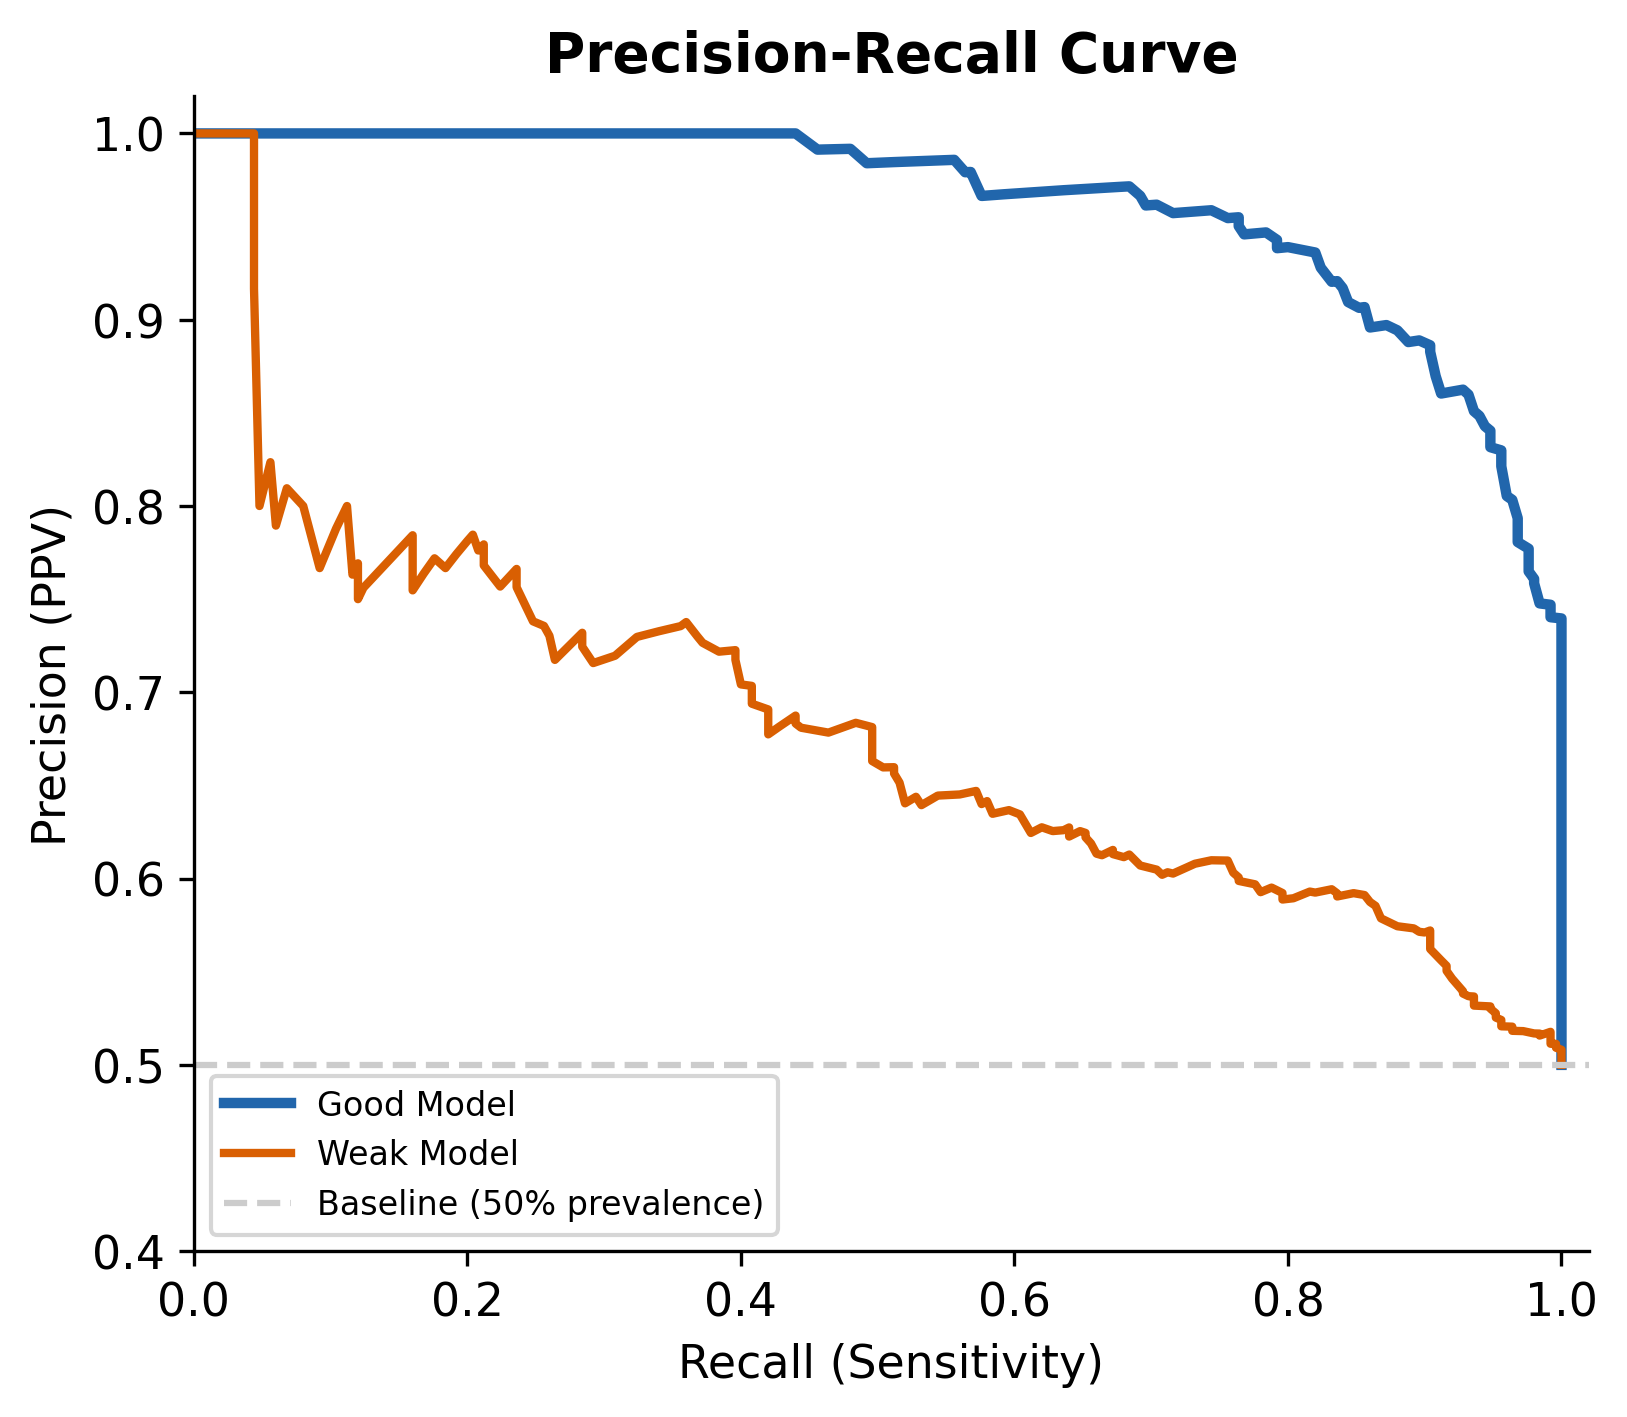
\includegraphics[width=0.62\textwidth]{m2_8_pr_curve.png}
\vspace{0.2cm}
\begin{columns}[T]
\begin{column}{0.48\textwidth}
\begin{itemize}
    \item $x$: Recall (Sensitivity)
    \item $y$: Precision (PPV)
    \item Better than ROC for \textbf{imbalanced} classes
    \item Baseline = prevalence (not 0.5)
\end{itemize}
\end{column}
\begin{column}{0.48\textwidth}
\begin{alertblock}{Pro-Tip}
    \scriptsize With 1\% positive rate, ROC looks good even for poor models. PR reveals the truth. Use PR for rare-event detection (fraud, disease screening).
\end{alertblock}
\end{column}
\end{columns}
\end{frame}

% ── 222 ──
\begin{frame}[fragile]{Precision-Recall --- Code}\smark{222/300}
\begin{columns}[T]
\begin{column}{0.48\textwidth}
\begin{lstlisting}[style=Rstyle]
library(yardstick)
pr_curve(df, truth, .pred_1) |>
  autoplot()

# PRROC package
library(PRROC)
pr <- pr.curve(
  scores.class0=scores[y==1],
  scores.class1=scores[y==0],
  curve=TRUE)
plot(pr)
\end{lstlisting}
\end{column}
\begin{column}{0.48\textwidth}
\begin{lstlisting}[style=Pystyle]
from sklearn.metrics import (
    PrecisionRecallDisplay,
    average_precision_score)

PrecisionRecallDisplay \
    .from_predictions(
        y_true, scores,
        name="Model")

ap = average_precision_score(
    y_true, scores)
print(f"AP = {ap:.3f}")
\end{lstlisting}
\end{column}
\end{columns}
\end{frame}

% ── 223 ──
\begin{frame}{Calibration Plot}\smark{223/300}
\centering
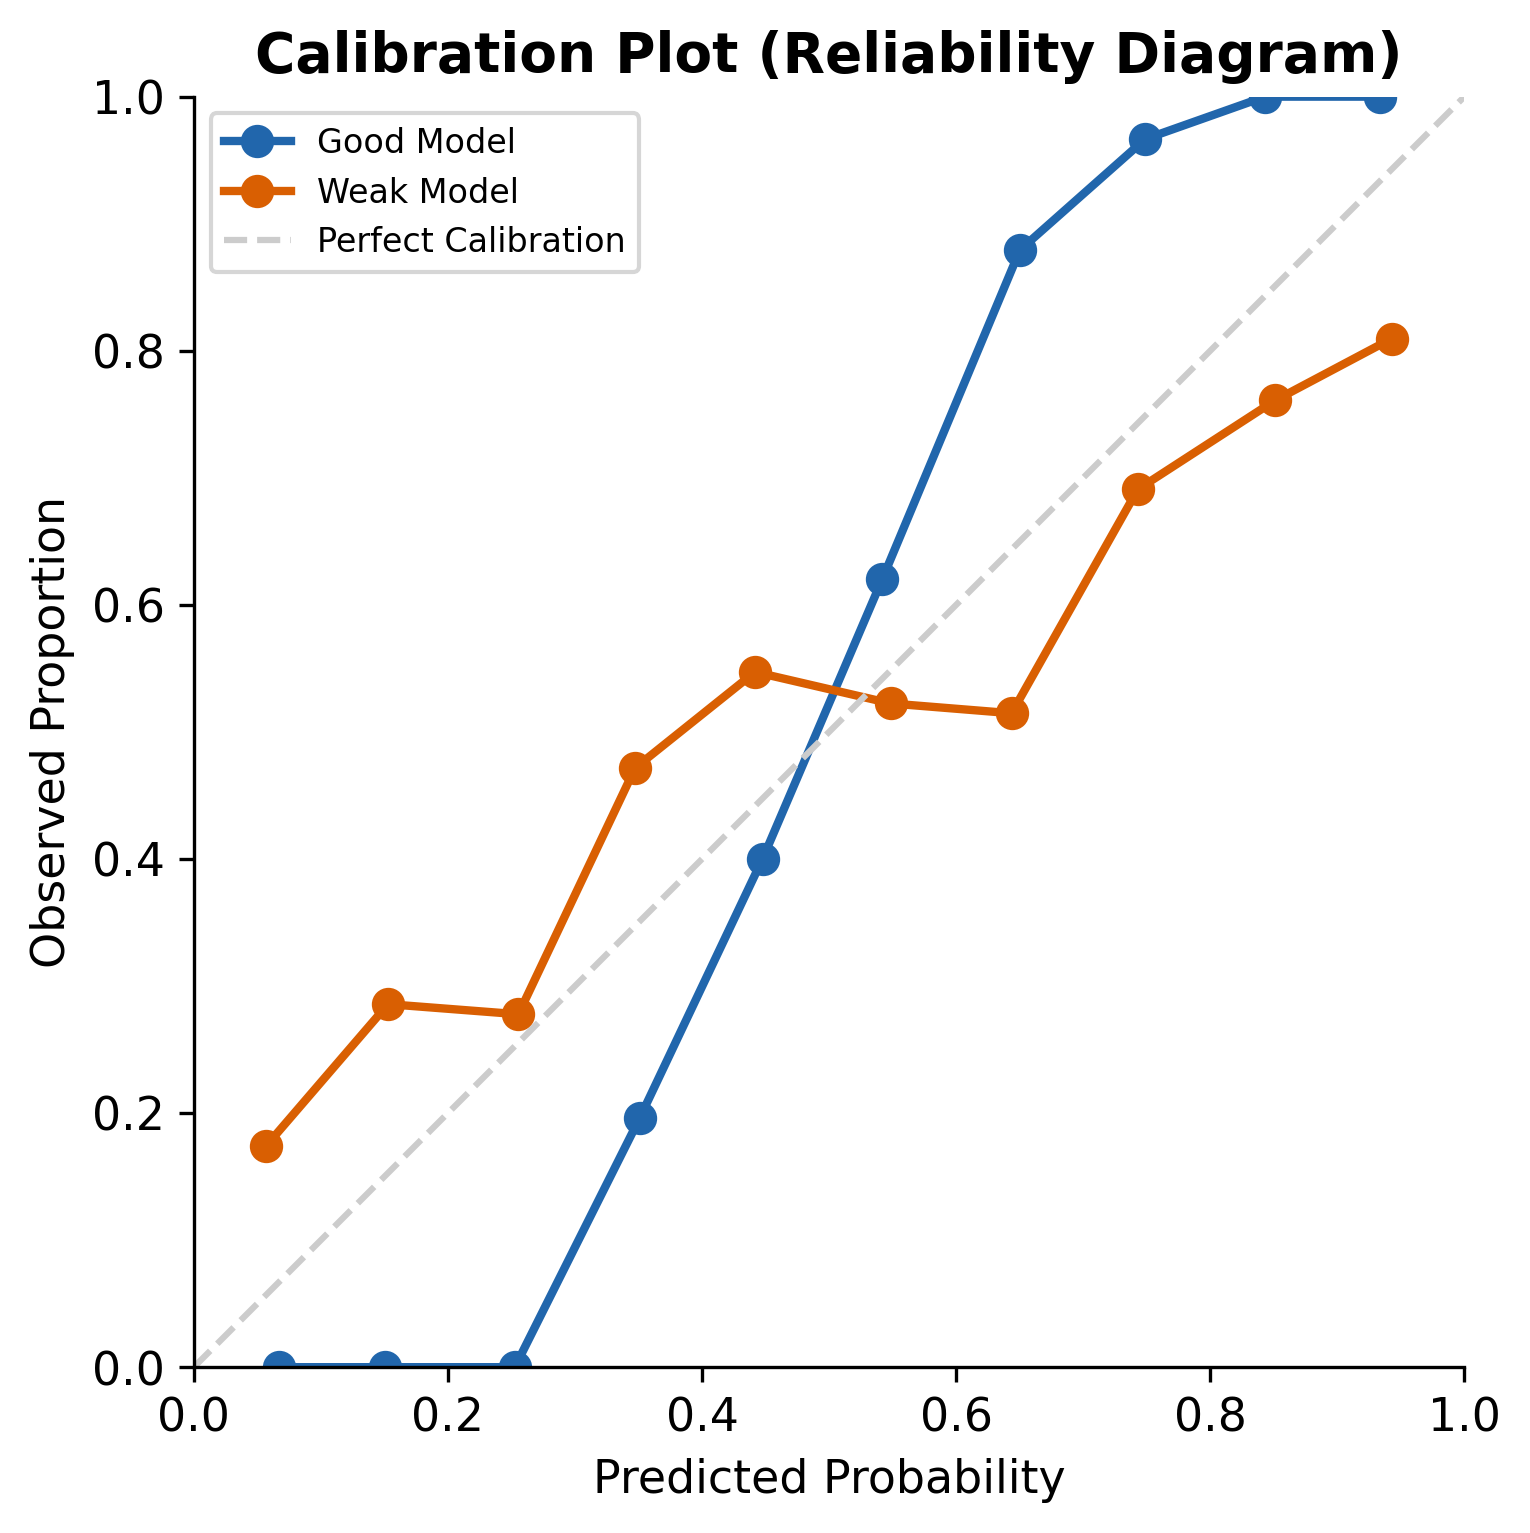
\includegraphics[width=0.58\textwidth]{m2_8_calibration.png}
\vspace{0.2cm}
\begin{columns}[T]
\begin{column}{0.48\textwidth}
\begin{itemize}
    \item $x$: predicted probability (binned)
    \item $y$: observed proportion of positives
    \item Diagonal = perfect calibration
    \item Above diagonal $\to$ under-confident
    \item Below $\to$ over-confident
\end{itemize}
\end{column}
\begin{column}{0.48\textwidth}
\begin{exampleblock}{Data Insight}
    \scriptsize A model can have high AUC but poor calibration. Calibration matters when the probability itself drives decisions --- medical risk, credit scoring.
\end{exampleblock}
\end{column}
\end{columns}
\end{frame}

% ── 224 ──
\begin{frame}[fragile]{Calibration --- Code}\smark{224/300}
\begin{columns}[T]
\begin{column}{0.48\textwidth}
\begin{lstlisting}[style=Rstyle]
df <- tibble(score=scores,y=y_true)|>
  mutate(bin=cut(score, 10)) |>
  group_by(bin) |>
  summarise(pred=mean(score),
            obs=mean(y))
ggplot(df, aes(pred, obs)) +
  geom_point(size=3) + geom_line() +
  geom_abline(linetype="dashed") +
  coord_equal(xlim=c(0,1),
    ylim=c(0,1)) +
  theme_minimal()
\end{lstlisting}
\end{column}
\begin{column}{0.48\textwidth}
\begin{lstlisting}[style=Pystyle]
from sklearn.calibration import (
    CalibrationDisplay)
CalibrationDisplay.from_predictions(
    y_true, scores, n_bins=10,
    name="Model")

# Fix with Platt scaling
from sklearn.calibration import \
    CalibratedClassifierCV
cal = CalibratedClassifierCV(
    model, method="sigmoid")
cal.fit(X_val, y_val)
\end{lstlisting}
\begin{alertblock}{Pro-Tip}
    \scriptsize Fix calibration with \texttt{CalibratedClassifierCV} (Platt scaling or isotonic regression) post-hoc.
\end{alertblock}
\end{column}
\end{columns}
\end{frame}

% ── 225 ──
\begin{frame}{Threshold Tuning}\smark{225/300}
\centering
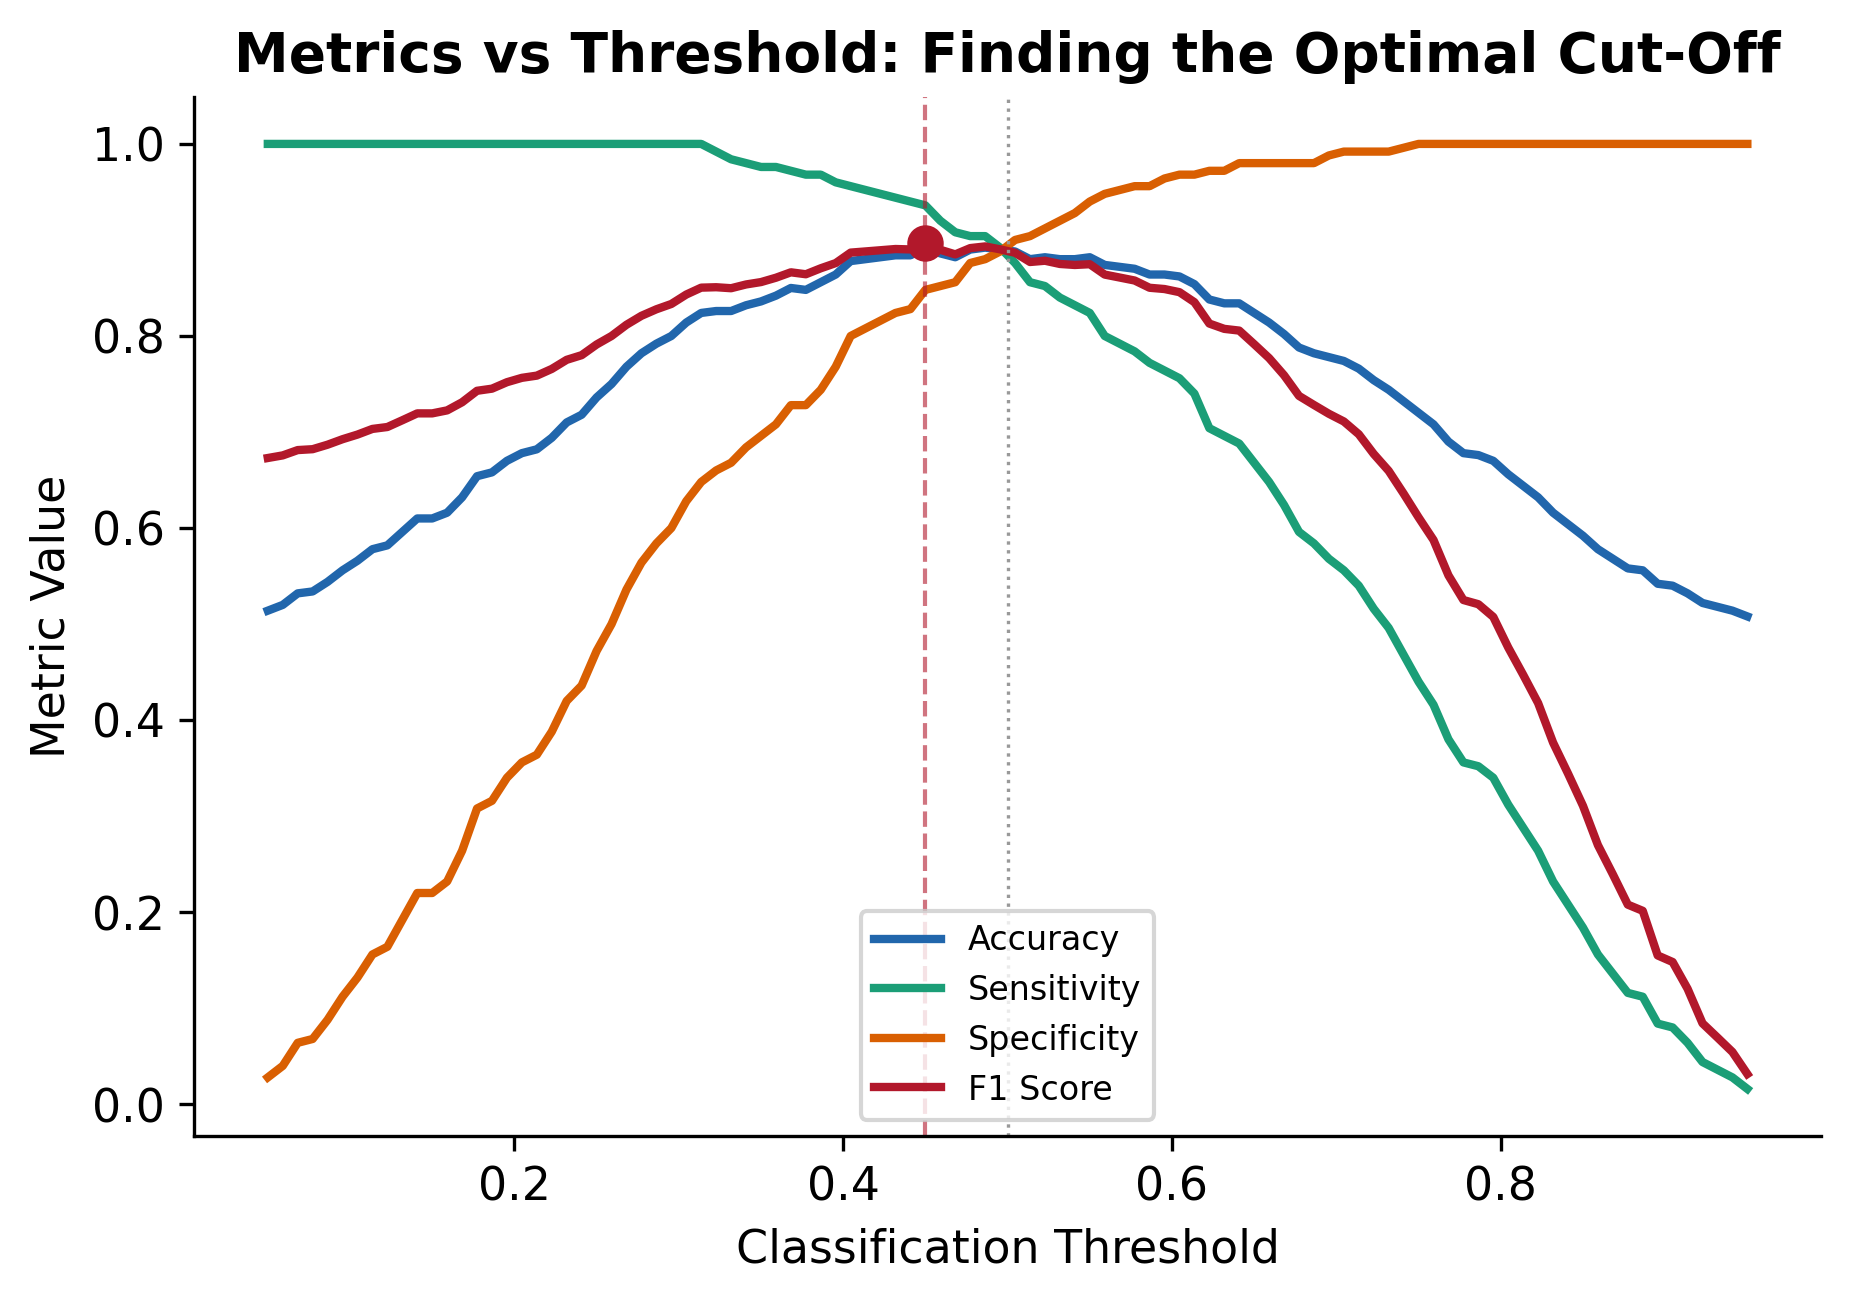
\includegraphics[width=0.72\textwidth]{m2_8_threshold_tuning.png}
\vspace{0.2cm}
\begin{columns}[T]
\begin{column}{0.48\textwidth}
\begin{itemize}
    \item Plot accuracy, sensitivity, specificity, F1 across thresholds
    \item Best threshold depends on \textbf{cost of errors}
    \item Medical: favour sensitivity (low threshold)
    \item Spam: favour precision (high threshold)
\end{itemize}
\end{column}
\begin{column}{0.48\textwidth}
\begin{exampleblock}{Data Insight}
    \scriptsize F1-optimal threshold (red dot) balances precision and recall. Clinical optimal may differ if missing disease is 10$\times$ worse than a false alarm.
\end{exampleblock}
\end{column}
\end{columns}
\end{frame}

% ── 226 ──
\begin{frame}[fragile]{Threshold Tuning --- Code}\smark{226/300}
\begin{columns}[T]
\begin{column}{0.48\textwidth}
\begin{lstlisting}[style=Rstyle]
thresholds <- seq(0.05, 0.95, 0.01)
metrics_df <- map_dfr(thresholds,
  function(t) {
    pred <- ifelse(scores>=t, 1, 0)
    tibble(threshold=t,
      acc=mean(pred==y),
      sens=sum(pred==1 & y==1)/
           sum(y==1),
      f1=f1_val)
  })
ggplot(metrics_df |>
  pivot_longer(-threshold),
  aes(threshold,value,color=name))+
  geom_line(linewidth=1) +
  theme_minimal()
\end{lstlisting}
\end{column}
\begin{column}{0.48\textwidth}
\begin{lstlisting}[style=Pystyle]
from sklearn.metrics import (
    accuracy_score, f1_score,
    recall_score)
thresholds = np.arange(0.05,0.95,0.01)
metrics = {"Acc":[],"Sens":[],"F1":[]}
for t in thresholds:
    pred = (scores>=t).astype(int)
    metrics["Acc"].append(
        accuracy_score(y_true, pred))
    metrics["Sens"].append(
        recall_score(y_true, pred))
    metrics["F1"].append(
        f1_score(y_true, pred))
for name, vals in metrics.items():
    ax.plot(thresholds, vals,
        label=name)
\end{lstlisting}
\end{column}
\end{columns}
\end{frame}

% ── 227 ──
\begin{frame}{Gain and Lift Charts}\smark{227/300}
\centering
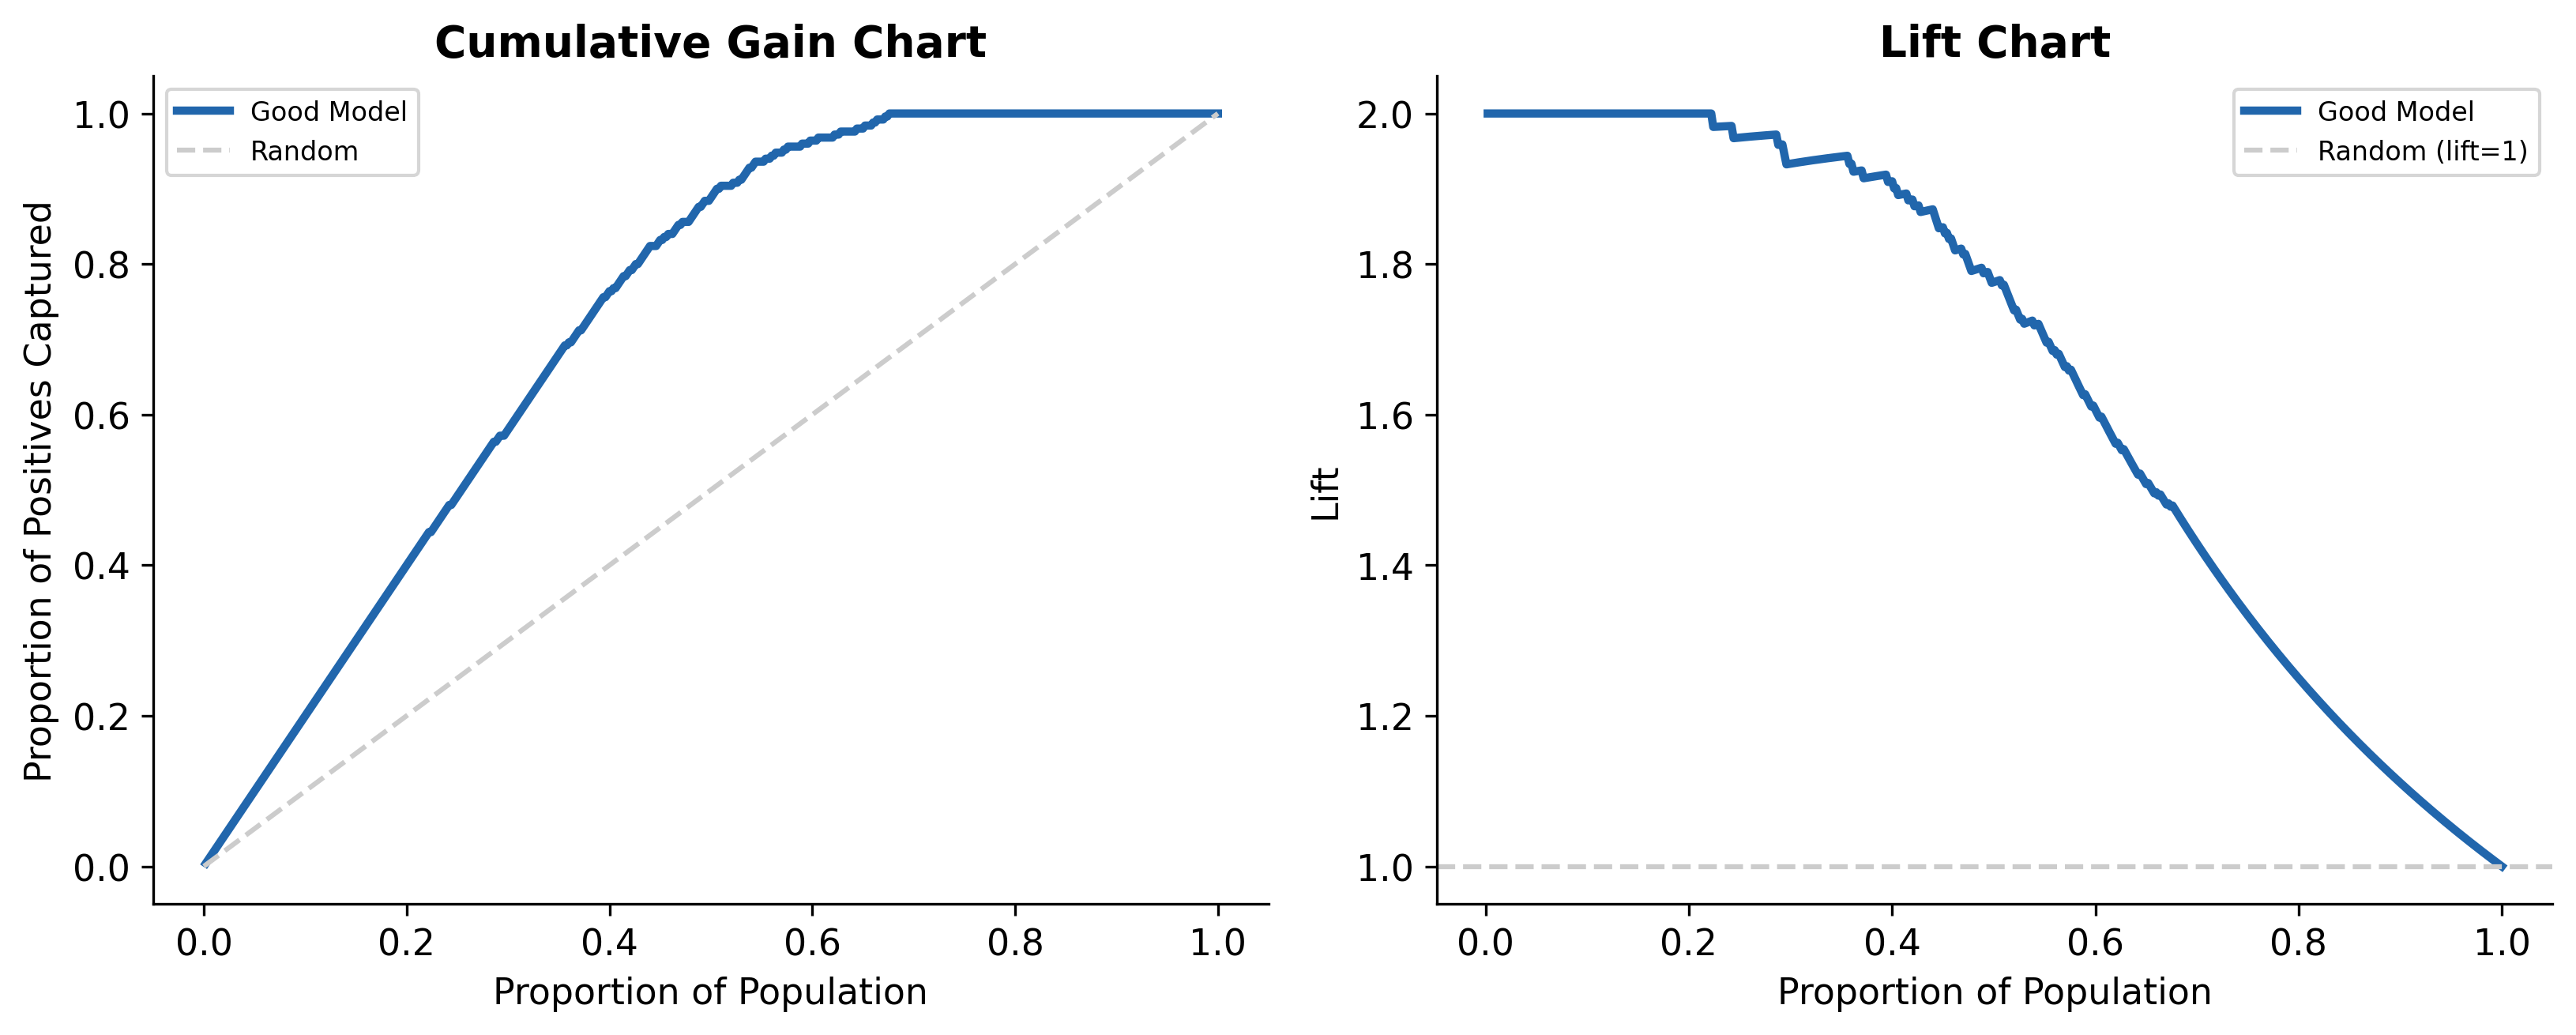
\includegraphics[width=0.88\textwidth]{m2_8_gain_lift.png}
\vspace{0.2cm}
\begin{columns}[T]
\begin{column}{0.48\textwidth}
\begin{exampleblock}{Data Insight}
    \scriptsize \textbf{Gain}: targeting top 20\% captures $\sim$60\% of positives. \textbf{Lift}: top 20\% gives 3$\times$ hit rate vs.\ random. Critical for marketing, fraud, screening.
\end{exampleblock}
\end{column}
\begin{column}{0.48\textwidth}
\begin{alertblock}{Pro-Tip}
    \scriptsize Gain/lift are business-facing. ROC/PR for modellers; gain/lift for decision-makers who ask ``how many cases to target?''
\end{alertblock}
\end{column}
\end{columns}
\end{frame}

% ── 228 ──
\begin{frame}[fragile]{Gain and Lift --- Code}\smark{228/300}
\begin{columns}[T]
\begin{column}{0.48\textwidth}
\begin{lstlisting}[style=Rstyle]
library(yardstick)
gain_curve(df, truth, .pred_1) |>
  autoplot()
lift_curve(df, truth, .pred_1) |>
  autoplot()
\end{lstlisting}
\end{column}
\begin{column}{0.48\textwidth}
\begin{lstlisting}[style=Pystyle]
order = np.argsort(-scores)
y_sorted = y_true[order]
cum_pos = np.cumsum(y_sorted)
gain = cum_pos / y_sorted.sum()
pop_frac = np.arange(1,n+1) / n
ax.plot(pop_frac, gain, color=B)
ax.plot([0,1],[0,1], "--", color="#CCC")
# Lift
lift = gain / pop_frac
ax.plot(pop_frac, lift)
ax.axhline(1, linestyle="--")
\end{lstlisting}
\end{column}
\end{columns}
\end{frame}

% ── 229 ──
\begin{frame}{Multi-Class Extensions}\smark{229/300}
\begin{columns}[T]
\begin{column}{0.50\textwidth}
\begin{itemize}
    \item Confusion: $k \times k$ grid
    \item ROC: one-vs-rest per class, macro/micro avg
    \item PR: one-vs-rest per class
    \item Normalize by row (recall) or column (precision)
\end{itemize}
\end{column}
\begin{column}{0.47\textwidth}
\begin{alertblock}{Pro-Tip}
    \scriptsize R: \texttt{yardstick::conf\_mat()} handles multi-class. Python: \texttt{normalize="true"} in \texttt{ConfusionMatrixDisplay} for row-normalized view.
\end{alertblock}
\end{column}
\end{columns}
\end{frame}

% ── 230 ──
\begin{frame}[fragile]{Multi-Class Confusion --- Code}\smark{230/300}
\begin{columns}[T]
\begin{column}{0.48\textwidth}
\begin{lstlisting}[style=Rstyle]
cm <- conf_mat(df, truth, estimate)
autoplot(cm, type="heatmap") +
  scale_fill_gradient(
    low="white", high="#2166AC")
summary(cm)
\end{lstlisting}
\end{column}
\begin{column}{0.48\textwidth}
\begin{lstlisting}[style=Pystyle]
ConfusionMatrixDisplay \
    .from_predictions(
        y_true, y_pred,
        normalize="true",
        cmap="Blues")
print(classification_report(
    y_true, y_pred))
\end{lstlisting}
\end{column}
\end{columns}
\end{frame}

% ── 231 ──
\begin{frame}{ROC vs.\ PR vs.\ Calibration: Decision Guide}\smark{231/300}
\centering\small
\begin{tabular}{@{}llll@{}}
    \toprule
    \textbf{Plot} & \textbf{Answers} & \textbf{Best When} & \textbf{Metric} \\
    \midrule
    ROC          & Can it rank?           & Balanced classes   & AUC-ROC \\
    PR           & Can it find positives? & Imbalanced classes & AUC-PR \\
    Calibration  & Are probs right?       & Decisions use $p$  & Brier score \\
    Score dist   & Is separation clean?   & Initial diagnosis  & (visual) \\
    Threshold    & What cut-off?          & Deployment         & F1, Youden \\
    Gain/Lift    & How many to target?    & Business context   & Lift at $k$\% \\
    \bottomrule
\end{tabular}
\vspace{0.2cm}
\begin{alertblock}{Pro-Tip}
    \scriptsize Present all three (ROC, PR, calibration) together. Each reveals a different failure mode.
\end{alertblock}
\end{frame}

% ── 232 ──
\begin{frame}{AUC Confidence Intervals}\smark{232/300}
\begin{columns}[T]
\begin{column}{0.50\textwidth}
\begin{itemize}
    \item AUC needs a CI (it is a point estimate)
    \item DeLong method: asymptotic, fast
    \item Bootstrap: 2{,}000+ resamples
    \item Compare models: paired DeLong or bootstrap difference
\end{itemize}
\end{column}
\begin{column}{0.47\textwidth}
\begin{alertblock}{Pro-Tip}
    \scriptsize R: \texttt{pROC::ci.auc(roc, method="delong")}. Python: bootstrap \texttt{roc\_auc\_score}. Always report AUC with CI.
\end{alertblock}
\end{column}
\end{columns}
\end{frame}

% ── 233 ──
\begin{frame}[fragile]{AUC CI --- Code}\smark{233/300}
\begin{columns}[T]
\begin{column}{0.48\textwidth}
\begin{lstlisting}[style=Rstyle]
library(pROC)
roc1 <- roc(y, scores1)
ci.auc(roc1)
# Compare two models
roc.test(roc1, roc2,
         method="delong")
\end{lstlisting}
\end{column}
\begin{column}{0.48\textwidth}
\begin{lstlisting}[style=Pystyle]
boot_aucs = []
for _ in range(2000):
    idx = np.random.choice(
        len(y_true), len(y_true),True)
    boot_aucs.append(roc_auc_score(
        y_true[idx], scores[idx]))
ci = np.percentile(boot_aucs,
    [2.5, 97.5])
\end{lstlisting}
\end{column}
\end{columns}
\end{frame}

% ── 234-236: Cost-sensitive threshold, DCA, DCA code ──
\begin{frame}{Cost-Sensitive Threshold Selection}\smark{234/300}
\begin{columns}[T]
\begin{column}{0.50\textwidth}
\begin{itemize}
    \item Default 0.5 is \textbf{rarely optimal}
    \item Youden's $J$: max(TPR $-$ FPR)
    \item Cost-weighted: min $C_{\text{FP}} \cdot \text{FP} + C_{\text{FN}} \cdot \text{FN}$
    \item Prevalence-adjusted for calibrated models
\end{itemize}
\end{column}
\begin{column}{0.47\textwidth}
\begin{alertblock}{Pro-Tip}
    \scriptsize R: \texttt{pROC::coords(roc, "best", best.method="youden")}. Python: \texttt{thresholds[np.argmax(tpr-fpr)]}.
\end{alertblock}
\end{column}
\end{columns}
\end{frame}

\begin{frame}{Decision Curve Analysis}\smark{235/300}
\begin{columns}[T]
\begin{column}{0.50\textwidth}
\begin{itemize}
    \item Evaluates clinical \textbf{net benefit} across thresholds
    \item Compares model to ``treat all'' and ``treat none''
    \item $x$: threshold probability; $y$: net benefit
    \item Required by TRIPOD+AI guidelines
\end{itemize}
\end{column}
\begin{column}{0.47\textwidth}
\begin{alertblock}{Pro-Tip}
    \scriptsize R: \texttt{dcurves::dca()}. Python: \texttt{dcurves} PyPI package. DCA incorporates cost ratios directly.
\end{alertblock}
\end{column}
\end{columns}
\end{frame}

\begin{frame}[fragile]{Decision Curve --- Code}\smark{236/300}
\begin{columns}[T]
\begin{column}{0.48\textwidth}
\begin{lstlisting}[style=Rstyle]
library(dcurves)
dca(outcome ~ model_pred,
    data=df,
    thresholds=seq(0,0.5,0.01)) |>
  plot(smooth=TRUE)
\end{lstlisting}
\end{column}
\begin{column}{0.48\textwidth}
\begin{lstlisting}[style=Pystyle]
from dcurves import dca, plot_graphs
dca_results = dca(data=df,
    outcome="outcome",
    modelnames=["model_pred"],
    thresholds=np.arange(0,0.5,0.01))
plot_graphs(plot_df=dca_results,
    graph_type="net_benefit")
\end{lstlisting}
\end{column}
\end{columns}
\end{frame}

% ── 237 ──
\begin{frame}{Classification Diagnostic Summary}\smark{237/300}
\centering\small
\begin{tabular}{@{}ll@{}}
    \toprule
    \textbf{Step} & \textbf{Plot} \\
    \midrule
    1. Score separation      & Score distributions by class \\
    2. Discrimination        & ROC (balanced) / PR (imbalanced) \\
    3. Calibration           & Reliability diagram + Brier \\
    4. Threshold             & Metrics-vs-threshold \\
    5. Error profile         & Confusion matrix \\
    6. Business translation  & Gain / lift \\
    7. Clinical decision     & Decision curve analysis \\
    \bottomrule
\end{tabular}
\end{frame}

% ── 238 ──
\begin{frame}{Common Mistakes}\smark{238/300}
\centering\small
\begin{tabular}{@{}ll@{}}
    \toprule
    \textbf{Mistake} & \textbf{Fix} \\
    \midrule
    ROC for imbalanced data          & Use PR curve \\
    AUC without CI                   & Bootstrap or DeLong \\
    Confusion without normalizing    & Row-normalize (recall) \\
    Threshold = 0.5 by default       & Tune to cost or Youden \\
    Accuracy for imbalanced          & F1, balanced acc, AUC-PR \\
    No calibration check             & Always plot for prob.\ models \\
    Train-set metrics only           & Evaluate on test set \\
    \bottomrule
\end{tabular}
\end{frame}

% ── 239 ──
\begin{frame}{Packages Reference}\smark{239/300}
\centering\small
\begin{tabular}{@{}lll@{}}
    \toprule
    \textbf{Task} & \textbf{R} & \textbf{Python} \\
    \midrule
    ROC / AUC      & \texttt{pROC}          & \texttt{sklearn.metrics} \\
    PR curve       & \texttt{PRROC}         & \texttt{sklearn.metrics} \\
    Confusion      & \texttt{yardstick}     & \texttt{sklearn.metrics} \\
    Calibration    & \texttt{probably}      & \texttt{sklearn.calibration} \\
    Decision curve & \texttt{dcurves}       & \texttt{dcurves} (PyPI) \\
    Gain / lift    & \texttt{yardstick}     & Manual / \texttt{scikitplot} \\
    \bottomrule
\end{tabular}
\end{frame}

% ── 240 ──
\begin{frame}{Module 2.8 --- Key Takeaways}\smark{240/300}
\begin{enumerate}
    \item \textbf{Score distributions} first: diagnose separation before metrics.
    \item \textbf{ROC} for balanced; \textbf{PR} for imbalanced.
    \item \textbf{Calibration} matters when decisions use the probability.
    \item \textbf{Threshold 0.5 is arbitrary.} Tune to cost or Youden's $J$.
    \item \textbf{AUC without CI} is incomplete.
    \item \textbf{Gain/lift} translate model quality into business decisions.
\end{enumerate}
\end{frame}

% ── 241 ──
\begin{frame}{}\smark{241/300}
\centering\vspace{1.5cm}
{\Large\textbf{Module 2.8 Complete}}\\[0.5cm]
You can now produce a complete classification diagnostic panel: score distributions, ROC, PR, calibration, threshold tuning, confusion matrix, gain/lift, and decision curve analysis.\\[0.5cm]
\textbf{Next:} Module 2.9 --- Residual Analysis for GLMs and Mixed Models.
\end{frame}

% % ═══════════════════════════════════════════════════════
%  MODULE 2.9 — Residual Analysis for GLMs and Mixed Models
% ═══════════════════════════════════════════════════════
\section{Module 2.9 --- GLM and Mixed-Model Residuals}

% ── 242 ──
\begin{frame}{Module 2.9 --- Roadmap}\smark{242/300}
\begin{enumerate}
    \item Why OLS residuals fail for GLMs
    \item Pearson, deviance, and quantile residuals
    \item Binned residual plots for logistic regression
    \item DHARMa: randomized quantile residuals + QQ
    \item Overdispersion diagnostics for count models
    \item Mixed models: caterpillar plots for random effects
    \item QQ plots of random effects
    \item Residuals by group: detecting heterogeneous variance
\end{enumerate}
\end{frame}

% ── 243 ──
\begin{frame}{Why OLS Residuals Fail for GLMs}
\smark{243/300}
\begin{columns}[T]
\begin{column}{0.50\textwidth}
\begin{itemize}
    \item OLS assumes $y \sim N(\mu, \sigma^2)$ with constant variance
    \item Poisson: $\text{Var}(y) = \mu$ (variance depends on mean)
    \item Binomial: $y \in \{0, 1\}$ --- residuals are not continuous
    \item Raw residuals $(y - \hat{y})$ show \textbf{structural patterns} even when the model is correct
    \item Need residual types that account for the GLM's variance function
\end{itemize}
\end{column}
\begin{column}{0.47\textwidth}
\begin{exampleblock}{Data Insight}
    \scriptsize For a Poisson GLM, raw residuals fan out (larger $\hat{\lambda}$ = larger variance). This is \emph{expected}, not a model failure. Pearson residuals divide by $\sqrt{\hat{\lambda}}$ to stabilize the variance.
\end{exampleblock}
\vspace{0.1cm}
\begin{alertblock}{Pro-Tip}
    \scriptsize Rule of thumb: use \textbf{deviance} residuals for plots and \textbf{Pearson} residuals for goodness-of-fit tests. Use \textbf{quantile} residuals (DHARMa) for the most reliable diagnostics.
\end{alertblock}
\end{column}
\end{columns}
\end{frame}

% ── 244 ──
\begin{frame}{Three Residual Types for GLMs}
\smark{244/300}
\centering
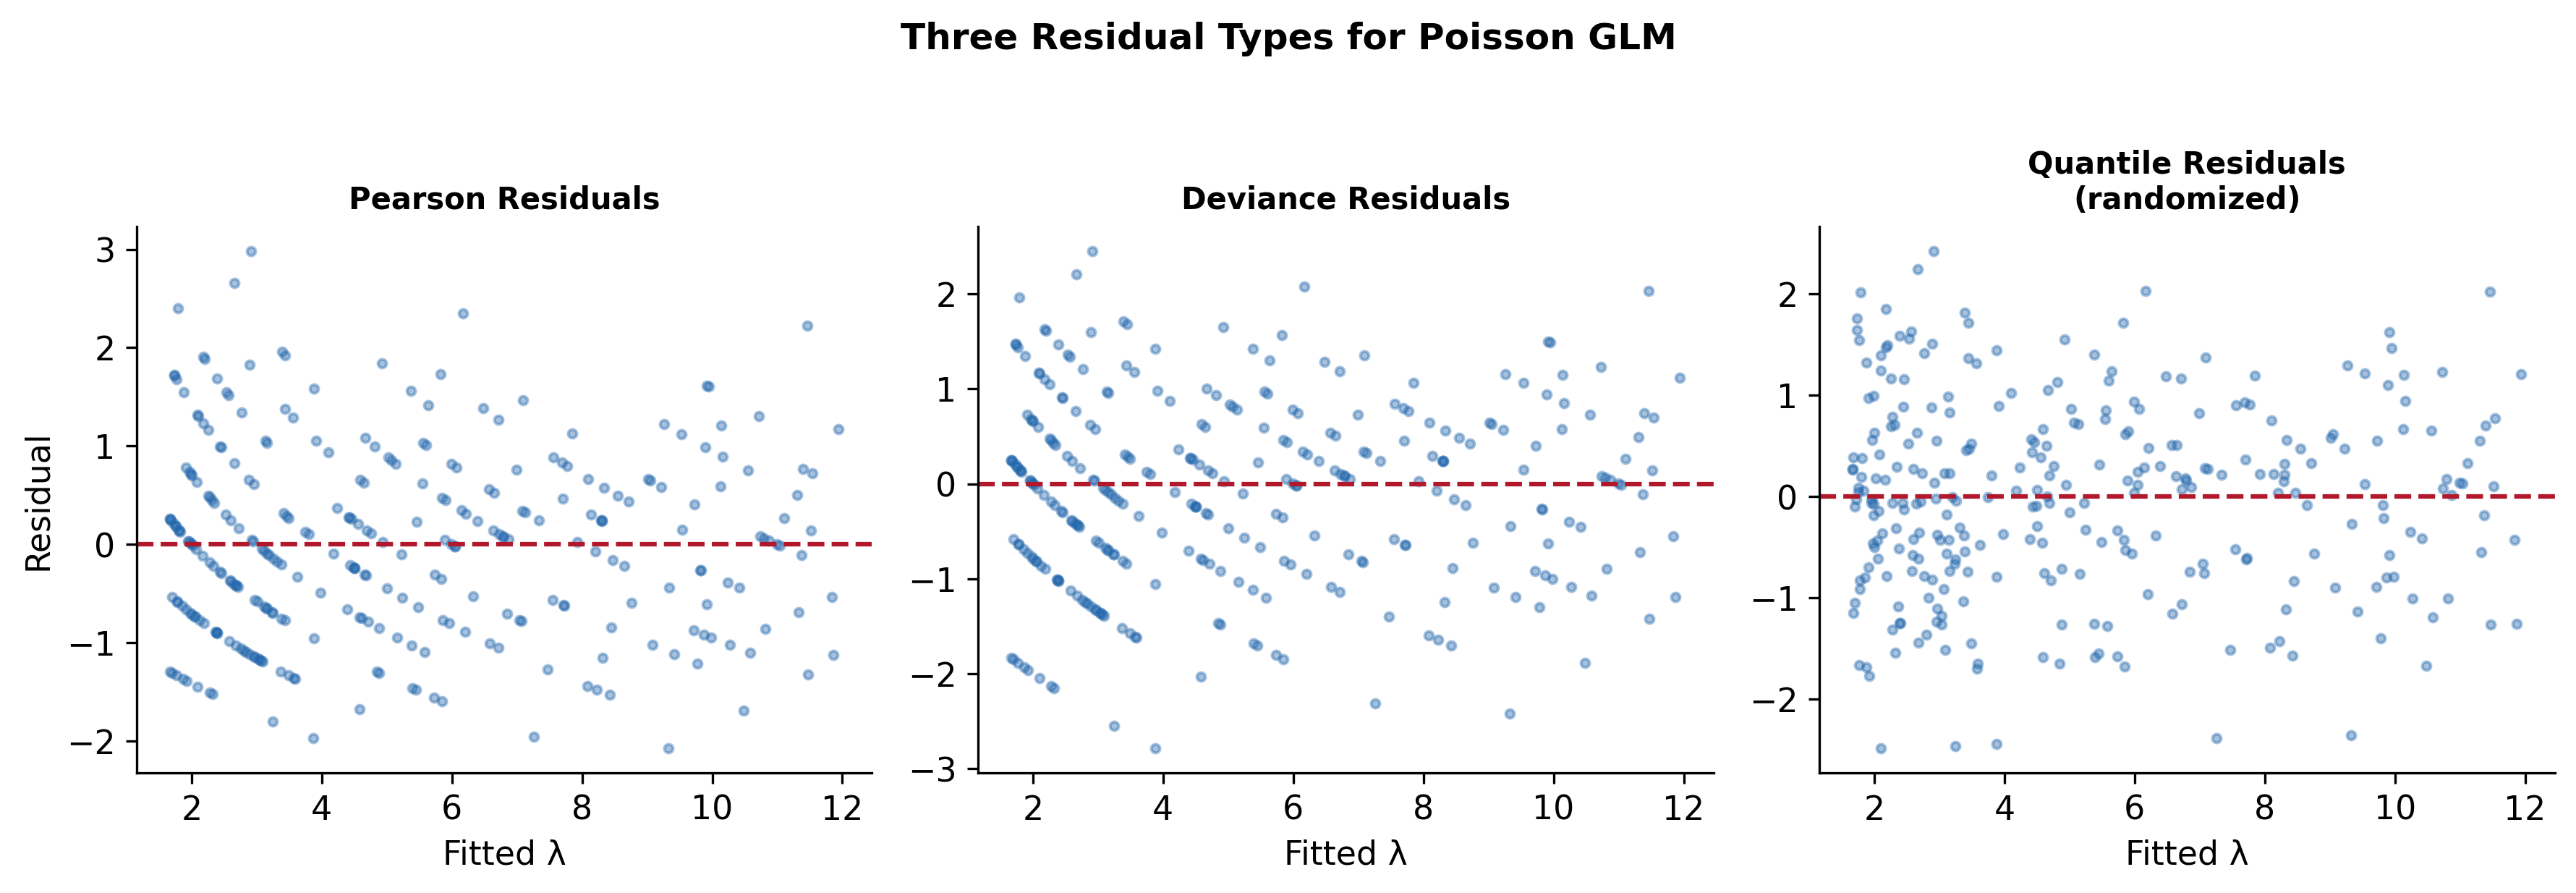
\includegraphics[width=0.88\textwidth]{m2_9_glm_residual_types.png}

\vspace{0.2cm}
\begin{exampleblock}{Data Insight}
    \scriptsize Pearson residuals (left) still show a slight fan. Deviance residuals (center) are better but not perfectly symmetric for discrete data. Quantile residuals (right) are exactly standard normal under the correct model --- the gold standard.
\end{exampleblock}
\end{frame}

% ── 245 ──
\begin{frame}{Residual Types: Formulas and Use Cases}
\smark{245/300}
\centering\small
\begin{tabular}{@{}llll@{}}
    \toprule
    \textbf{Type} & \textbf{Formula} & \textbf{Good For} & \textbf{Limitation} \\
    \midrule
    Raw        & $y_i - \hat{\mu}_i$                            & Quick look      & Structural patterns \\
    Pearson    & $(y_i - \hat{\mu}_i) / \sqrt{V(\hat{\mu}_i)}$  & GOF tests       & Not exactly normal \\
    Deviance   & $\text{sign}(y_i-\hat{\mu}_i) \sqrt{d_i}$     & Diagnostic plots & Discrete artifacts \\
    Quantile   & $\Phi^{-1}(F(y_i | \hat{\mu}_i))$             & QQ plots, DHARMa & Requires simulation \\
    \bottomrule
\end{tabular}

\vspace{0.3cm}
\begin{alertblock}{Pro-Tip}
    \scriptsize Quantile residuals (Dunn \& Smyth, 1996) transform through the fitted CDF. Under the correct model, they are exactly $N(0,1)$ --- standard QQ and residual-vs-fitted plots work as usual.
\end{alertblock}
\end{frame}

% ── 246 ──
\begin{frame}[fragile]{GLM Residuals --- \Rlang}\smark{246/300}
\begin{columns}[T]
\begin{column}{0.55\textwidth}
\begin{lstlisting}[style=Rstyle]
model <- glm(count ~ x,
  family = poisson, data = df)

# Pearson residuals
r_pearson <- residuals(model,
  type = "pearson")

# Deviance residuals (default)
r_deviance <- residuals(model,
  type = "deviance")

# Quantile residuals (statmod)
library(statmod)
r_quantile <- qresiduals(model)

# Plot
plot(fitted(model), r_deviance)
abline(h = 0, lty = 2, col = "red")
\end{lstlisting}
\end{column}
\begin{column}{0.42\textwidth}
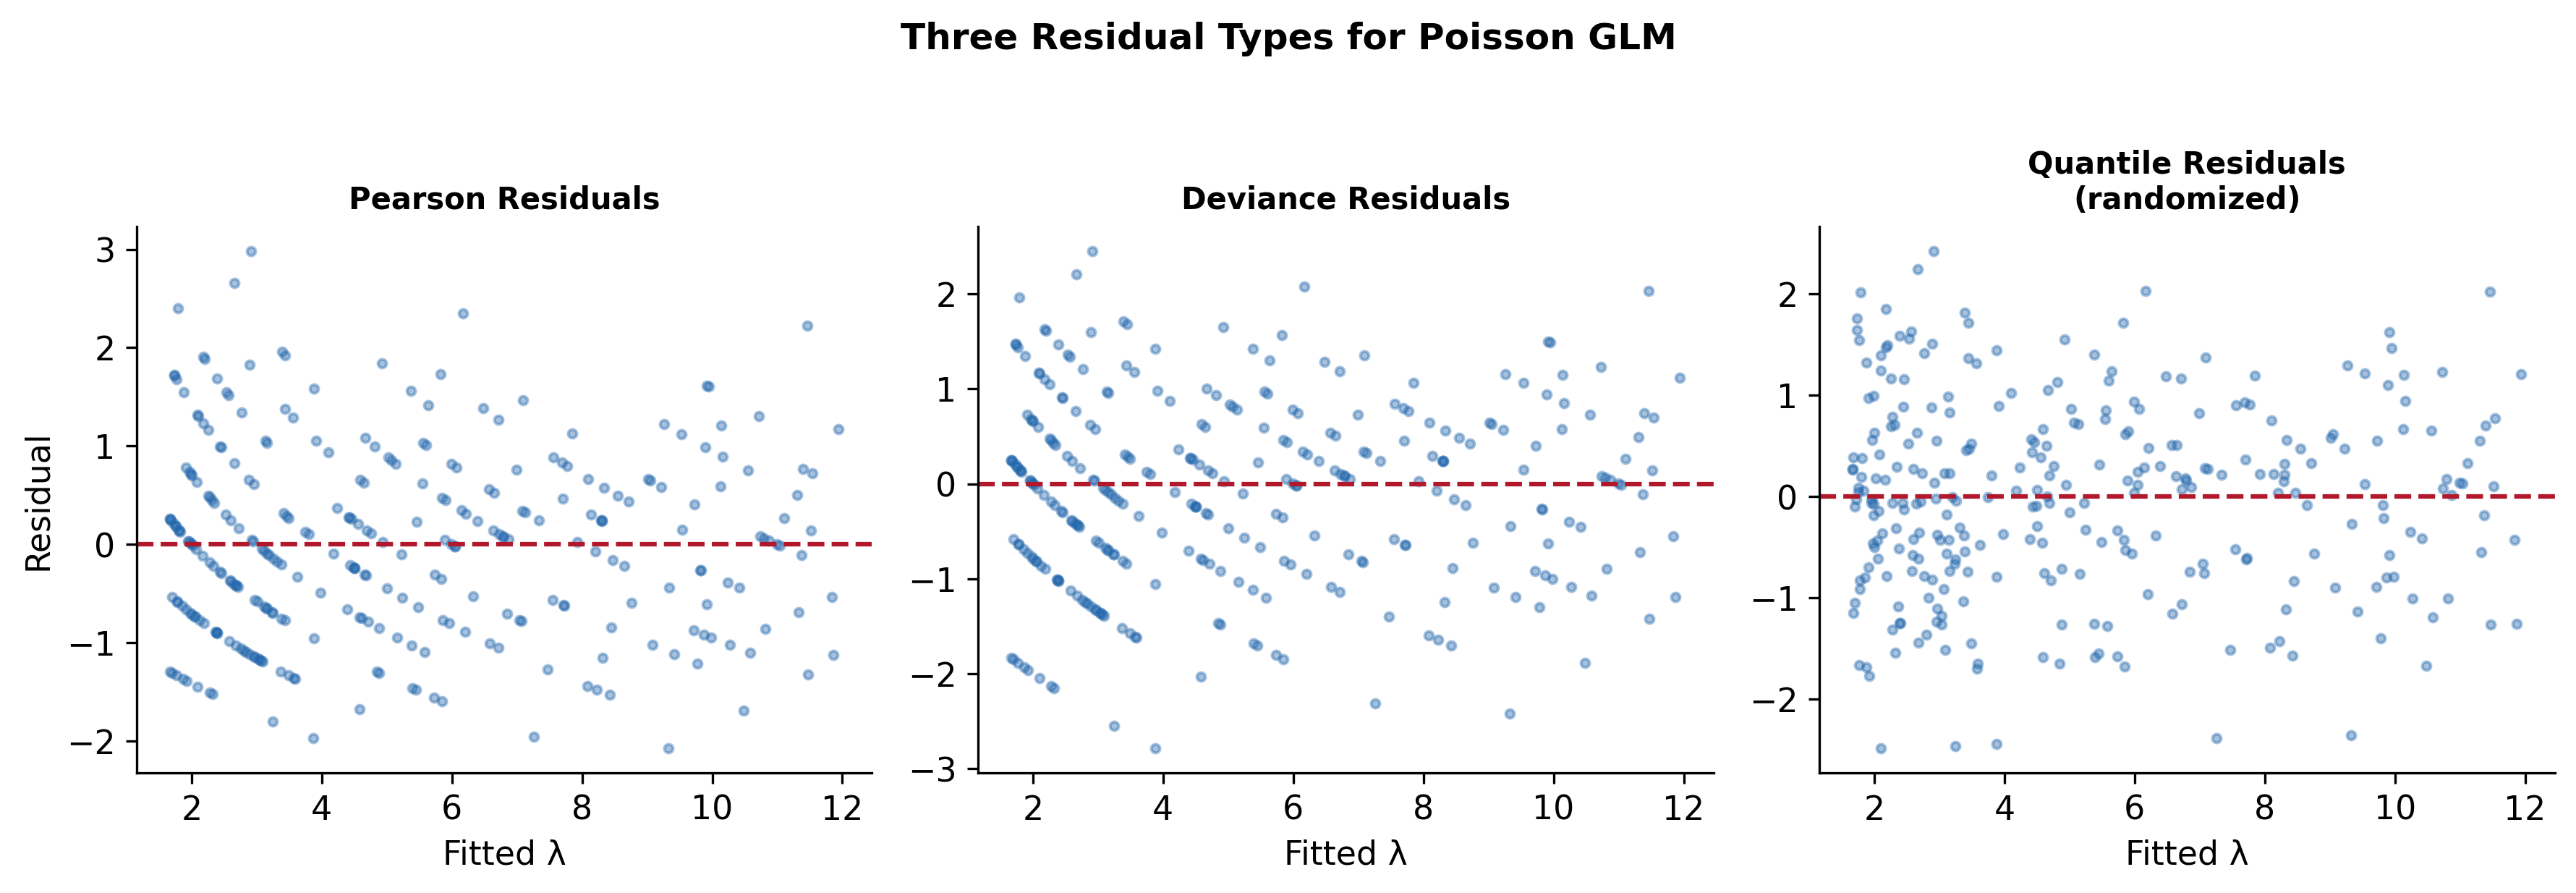
\includegraphics[width=\textwidth]{m2_9_glm_residual_types.png}
\begin{exampleblock}{Data Insight}
    \scriptsize \texttt{residuals(model, type=)} selects the type. Default is \texttt{"deviance"} for GLMs. \texttt{statmod::qresiduals()} provides quantile residuals.
\end{exampleblock}
\end{column}
\end{columns}
\end{frame}

% ── 247 ──
\begin{frame}[fragile]{GLM Residuals --- \Python}\smark{247/300}
\begin{columns}[T]
\begin{column}{0.55\textwidth}
\begin{lstlisting}[style=Pystyle]
import statsmodels.api as sm

model = sm.GLM(y, X,
    family=sm.families.Poisson()
    ).fit()

# Pearson
r_pearson = model.resid_pearson

# Deviance
r_deviance = model.resid_deviance

# Quantile (manual)
from scipy.stats import poisson, norm
u = np.array([
    np.random.uniform(
        poisson.cdf(max(yi-1,0), li),
        poisson.cdf(yi, li))
    for yi, li in zip(y, model.mu)])
r_quantile = norm.ppf(u)

ax.scatter(model.mu, r_deviance, s=8)
\end{lstlisting}
\end{column}
\begin{column}{0.42\textwidth}
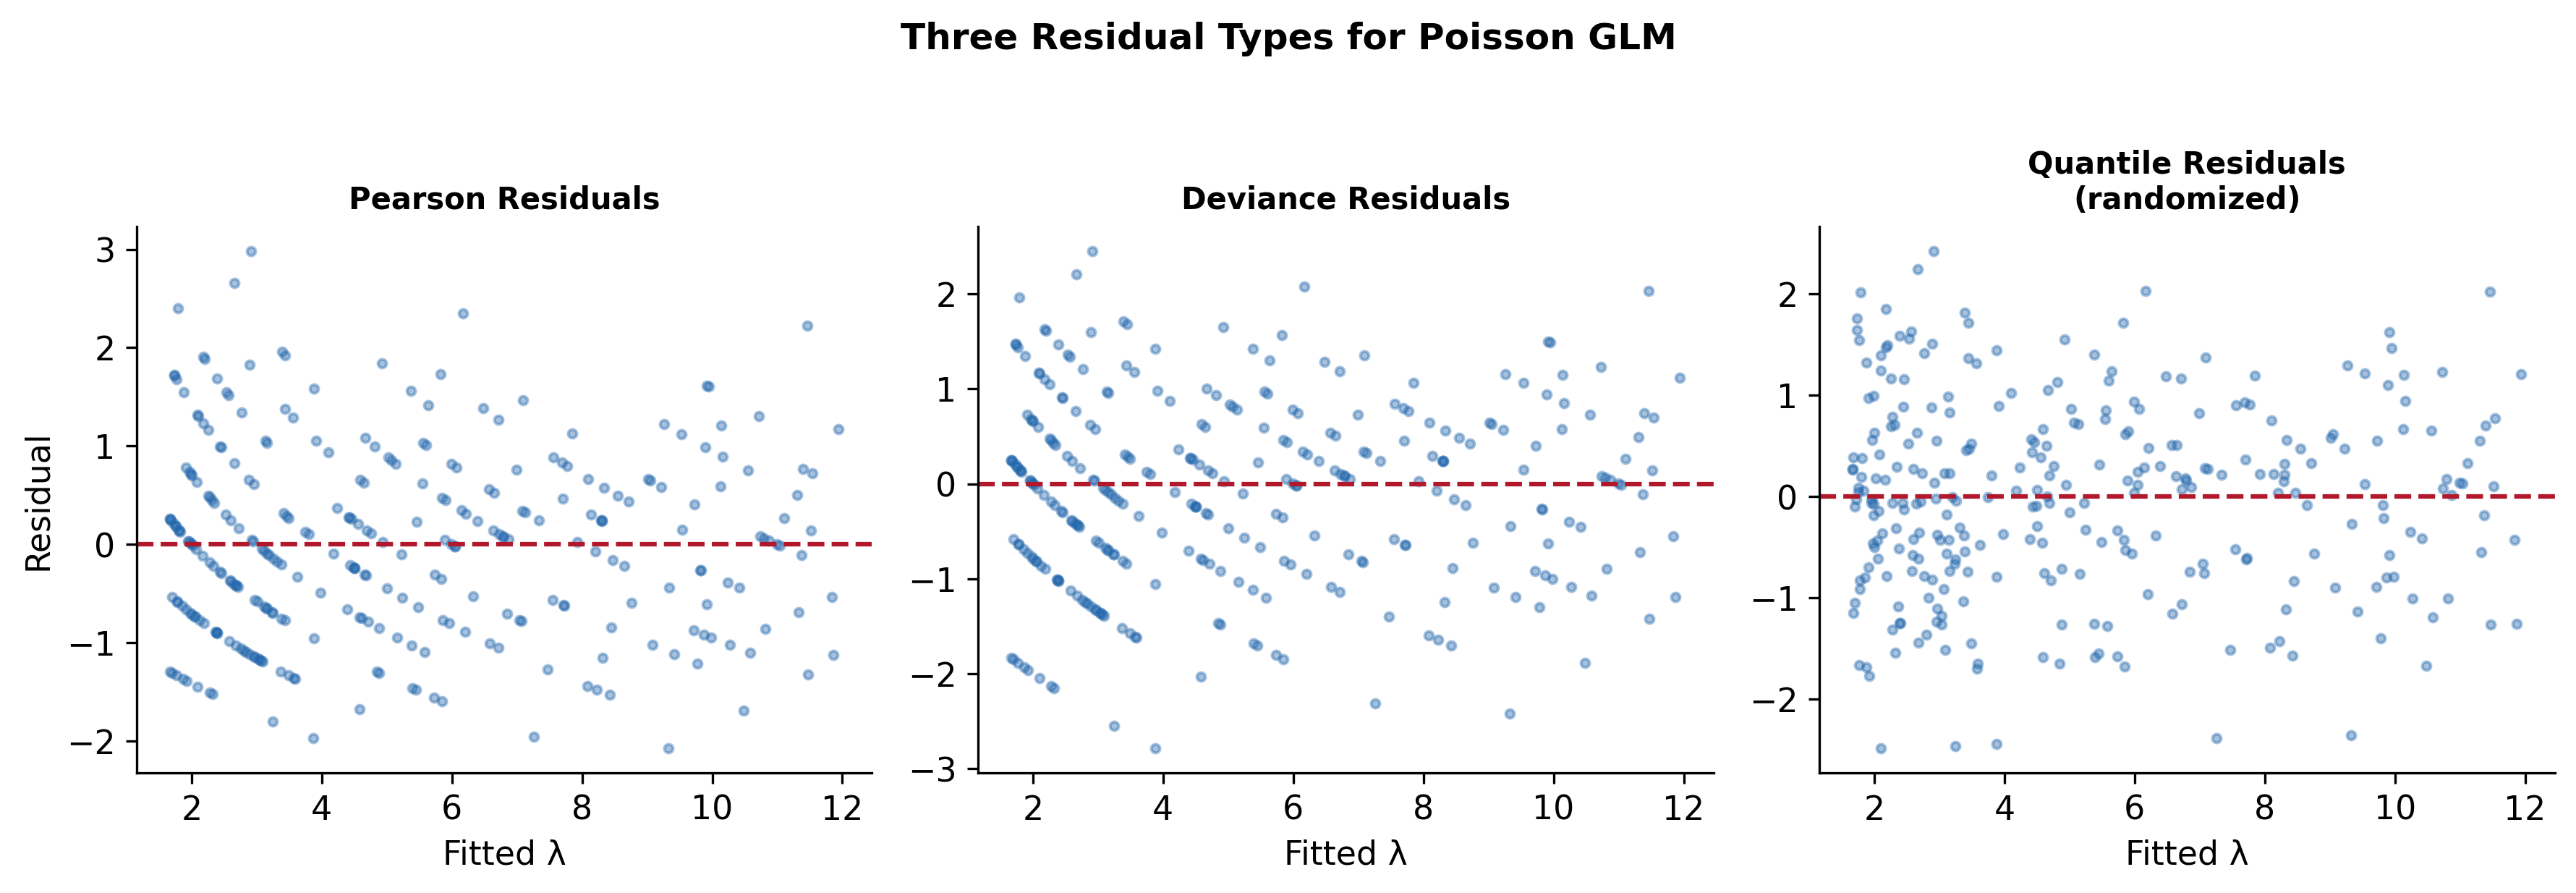
\includegraphics[width=\textwidth]{m2_9_glm_residual_types.png}
\begin{alertblock}{Pro-Tip}
    \scriptsize statsmodels provides \texttt{resid\_pearson} and \texttt{resid\_deviance} directly. Quantile residuals require manual computation via the CDF --- or use the \texttt{statsmodels.genmod} QQ tools.
\end{alertblock}
\end{column}
\end{columns}
\end{frame}

% ── 248 ──
\begin{frame}{Binned Residual Plot for Logistic Regression}
\smark{248/300}
\centering
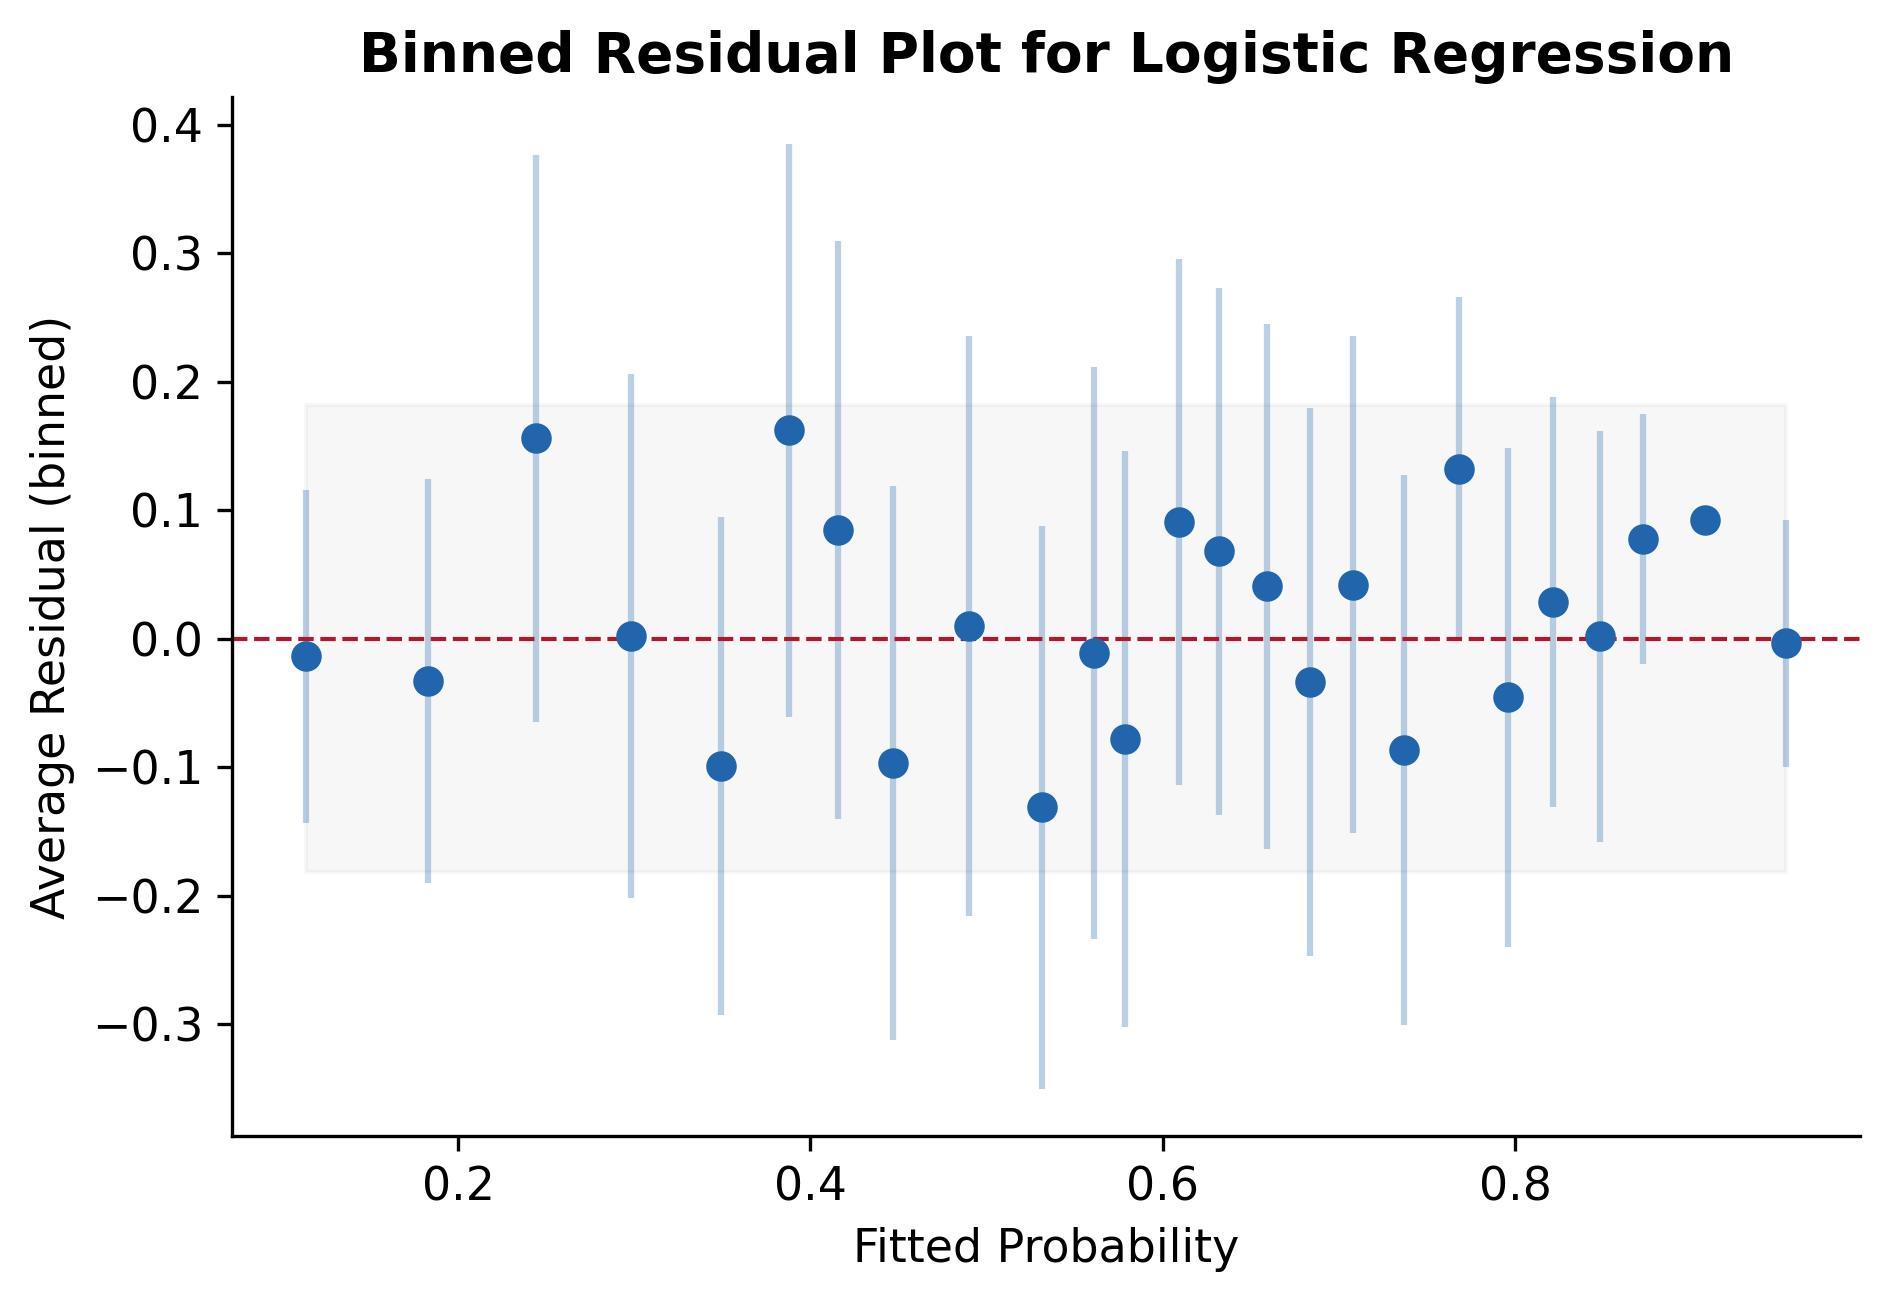
\includegraphics[width=0.72\textwidth]{m2_9_binned_residual.png}

\vspace{0.2cm}
\begin{columns}[T]
\begin{column}{0.48\textwidth}
\begin{itemize}
    \item Raw logistic residuals are 0 or 1 minus $\hat{p}$ --- uninformative when plotted individually
    \item \textbf{Bin} observations by $\hat{p}$, compute mean residual per bin
    \item Points should scatter within the $\pm 2\text{SE}$ band
    \item Systematic departure = misspecification
\end{itemize}
\end{column}
\begin{column}{0.48\textwidth}
\begin{alertblock}{Pro-Tip}
    \scriptsize R: \texttt{arm::binnedplot(fitted(model), resid(model))}. The function auto-bins and adds the 2SE band. Python: manual binning with \texttt{np.digitize()}.
\end{alertblock}
\end{column}
\end{columns}
\end{frame}

% ── 249 ──
\begin{frame}[fragile]{Binned Residual --- Code}\smark{249/300}
\begin{columns}[T]
\begin{column}{0.48\textwidth}
\begin{lstlisting}[style=Rstyle]
library(arm)

model <- glm(y ~ x1 + x2,
  family = binomial, data = df)

# One-liner
binnedplot(fitted(model),
           resid(model, type="response"),
           nclass = 25)

# ggplot2 manual approach
df_binned <- tibble(
  fitted = fitted(model),
  resid = resid(model)) |>
  mutate(bin = ntile(fitted, 25)) |>
  group_by(bin) |>
  summarise(mean_fitted=mean(fitted),
            mean_resid=mean(resid),
            se=sd(resid)/sqrt(n()))
\end{lstlisting}
\end{column}
\begin{column}{0.48\textwidth}
\begin{lstlisting}[style=Pystyle]
# Manual binned residual
p_hat = model.predict()
resid = y - p_hat
n_bins = 25
order = np.argsort(p_hat)
bin_size = len(y) // n_bins

bin_x, bin_r = [], []
for i in range(n_bins):
    idx = order[i*bin_size:
                (i+1)*bin_size]
    bin_x.append(p_hat[idx].mean())
    bin_r.append(resid[idx].mean())

ax.scatter(bin_x, bin_r)
ax.axhline(0, linestyle="--",
    color="#B2182B")
\end{lstlisting}
\end{column}
\end{columns}
\end{frame}

% ── 250 ──
\begin{frame}{DHARMa: Simulation-Based Diagnostics}
\smark{250/300}
\centering
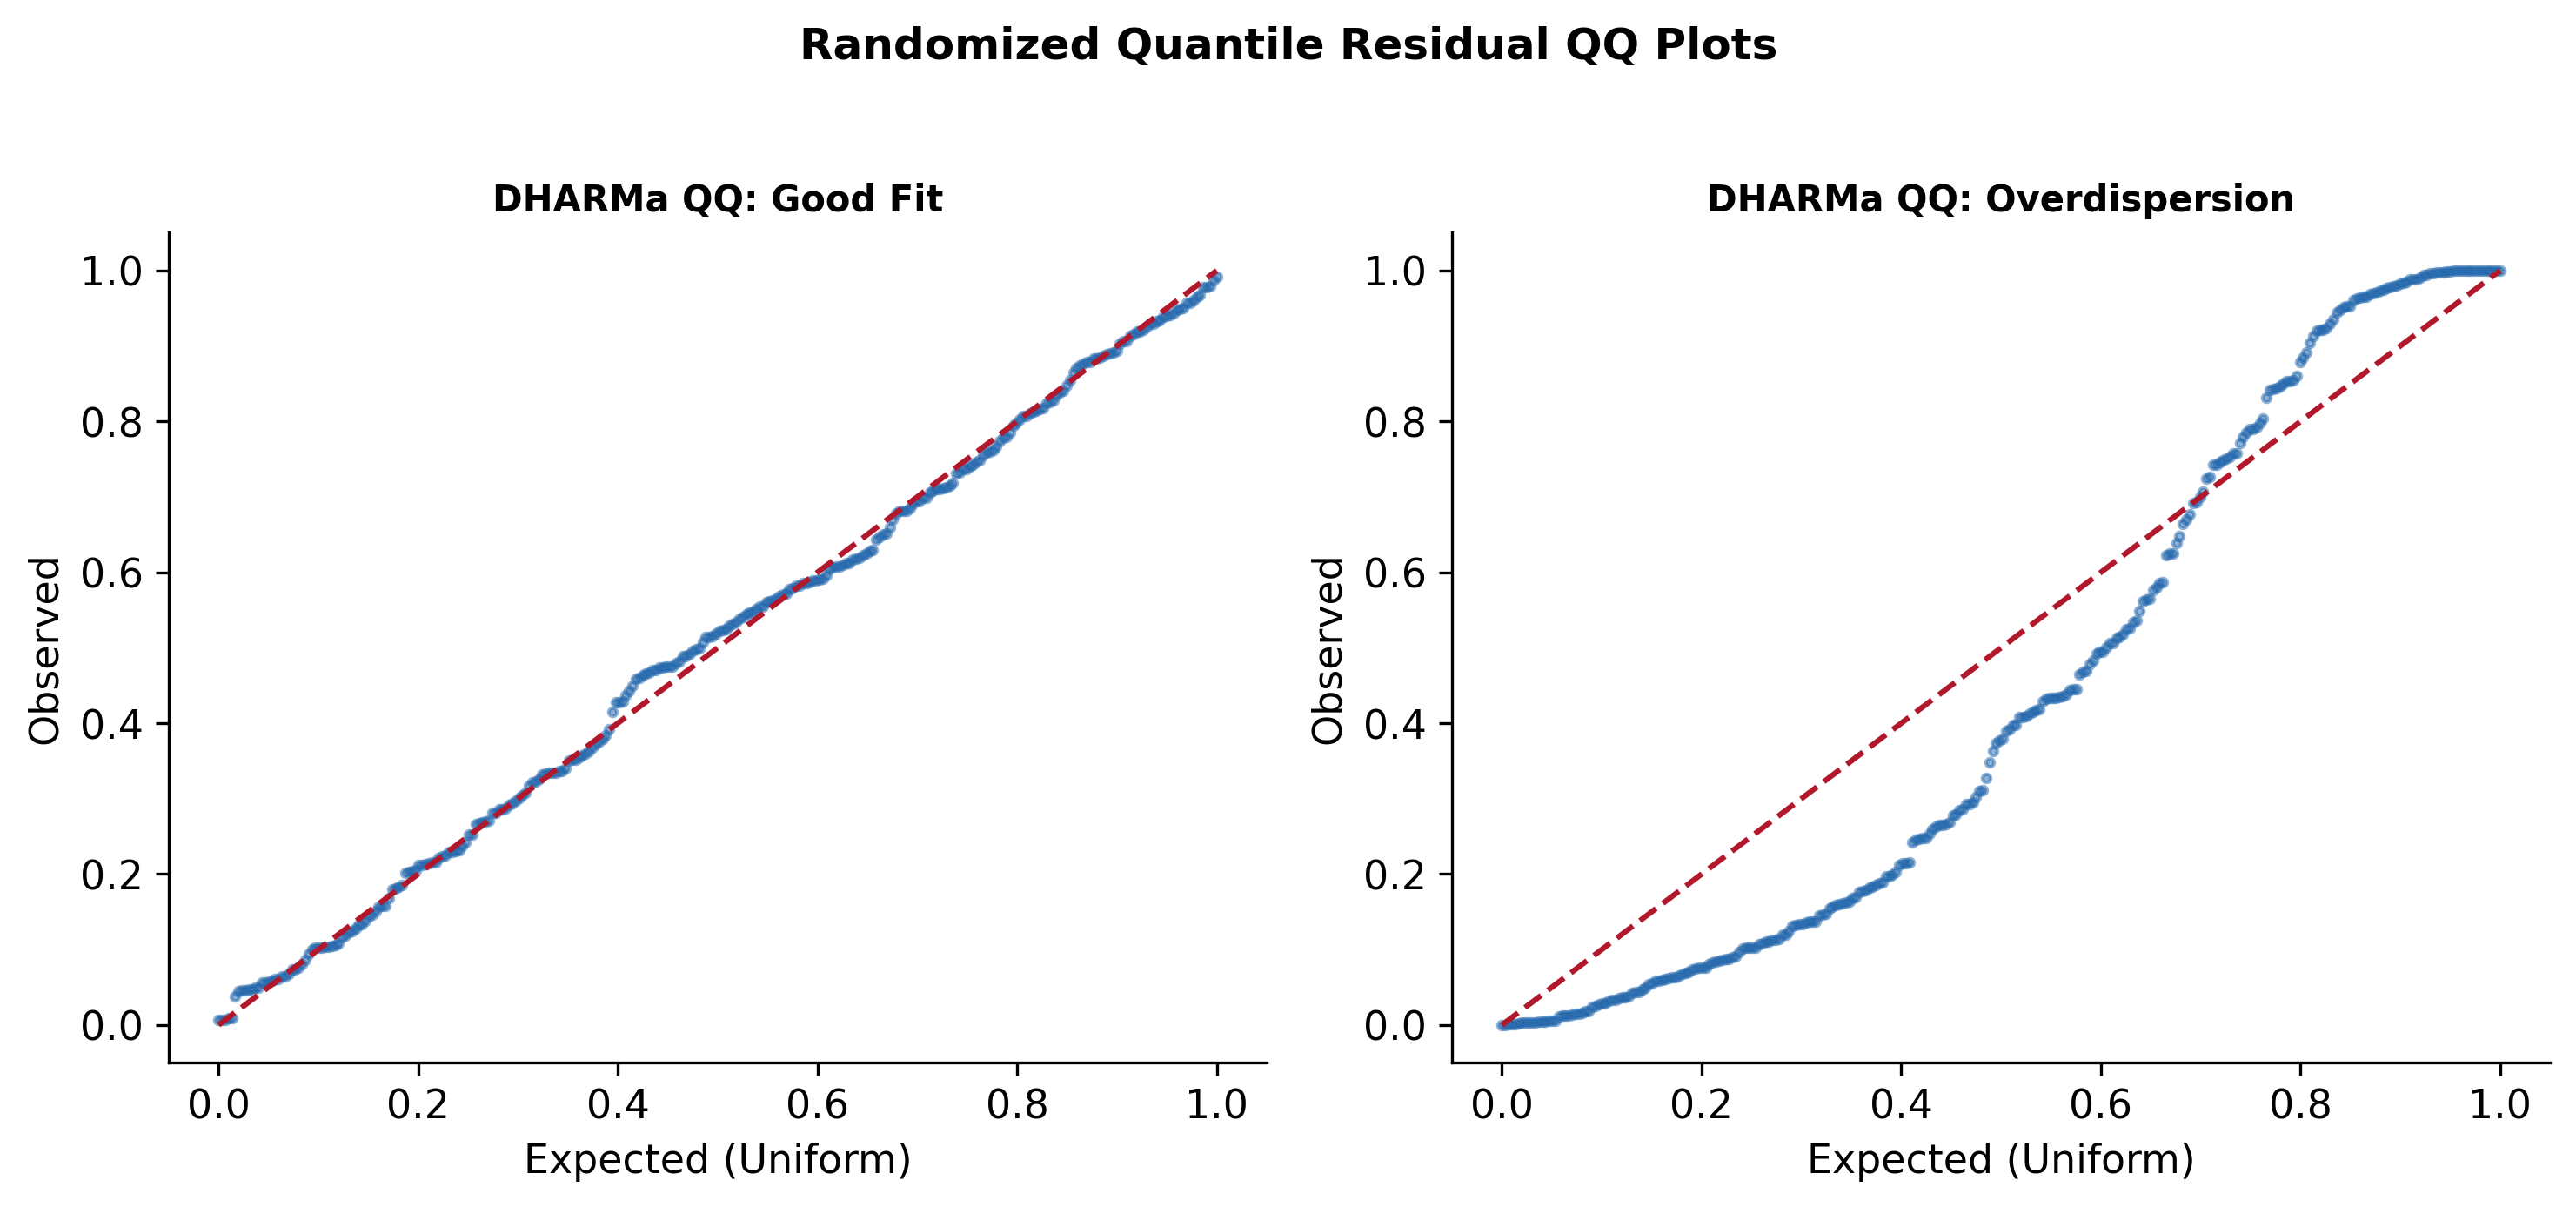
\includegraphics[width=0.85\textwidth]{m2_9_dharma_qq.png}

\vspace{0.2cm}
\begin{columns}[T]
\begin{column}{0.48\textwidth}
\begin{itemize}
    \item Simulates data from the fitted model $B$ times
    \item Computes CDF-based quantile residuals
    \item Under correct model: residuals $\sim \text{Uniform}(0,1)$
    \item QQ plot against uniform: deviations = misfit
    \item Works for \textbf{any} model: GLM, GLMM, GAM, zero-inflated
\end{itemize}
\end{column}
\begin{column}{0.48\textwidth}
\begin{exampleblock}{Data Insight}
    \scriptsize Left: correct Poisson model --- points hug the diagonal. Right: negative binomial data fit with Poisson --- the S-curve reveals overdispersion (tails heavier than expected).
\end{exampleblock}
\end{column}
\end{columns}
\end{frame}

% ── 251 ──
\begin{frame}[fragile]{DHARMa --- Code}\smark{251/300}
\begin{columns}[T]
\begin{column}{0.48\textwidth}
\begin{lstlisting}[style=Rstyle]
library(DHARMa)

model <- glm(count ~ x,
  family = poisson, data = df)

# Simulate residuals
sim_res <- simulateResiduals(
  fittedModel = model,
  n = 1000)

# Standard diagnostic panel
plot(sim_res)
# QQ + resid vs fitted

# Individual tests
testDispersion(sim_res)
testZeroInflation(sim_res)
testOutliers(sim_res)
\end{lstlisting}
\end{column}
\begin{column}{0.48\textwidth}
\begin{lstlisting}[style=Pystyle]
# No direct DHARMa in Python.
# Manual approach:
# 1. Simulate n_sim datasets
# 2. For each obs, compute rank
#    of y_i among simulated values

n_sim = 1000
simulated = np.random.poisson(
    model.mu[:, None],
    size=(len(y), n_sim))
# Quantile = proportion of sims <= y
quantiles = np.mean(
    simulated <= y[:, None], axis=1)
# Add jitter for discrete data
quantiles += np.random.uniform(
    0, 1/n_sim, len(y))

# QQ against uniform
from scipy.stats import probplot
probplot(quantiles, dist="uniform",
    plot=ax)
\end{lstlisting}
\end{column}
\end{columns}
\end{frame}

% ── 252 ──
\begin{frame}{Overdispersion: Diagnosis and Solutions}
\smark{252/300}
\centering
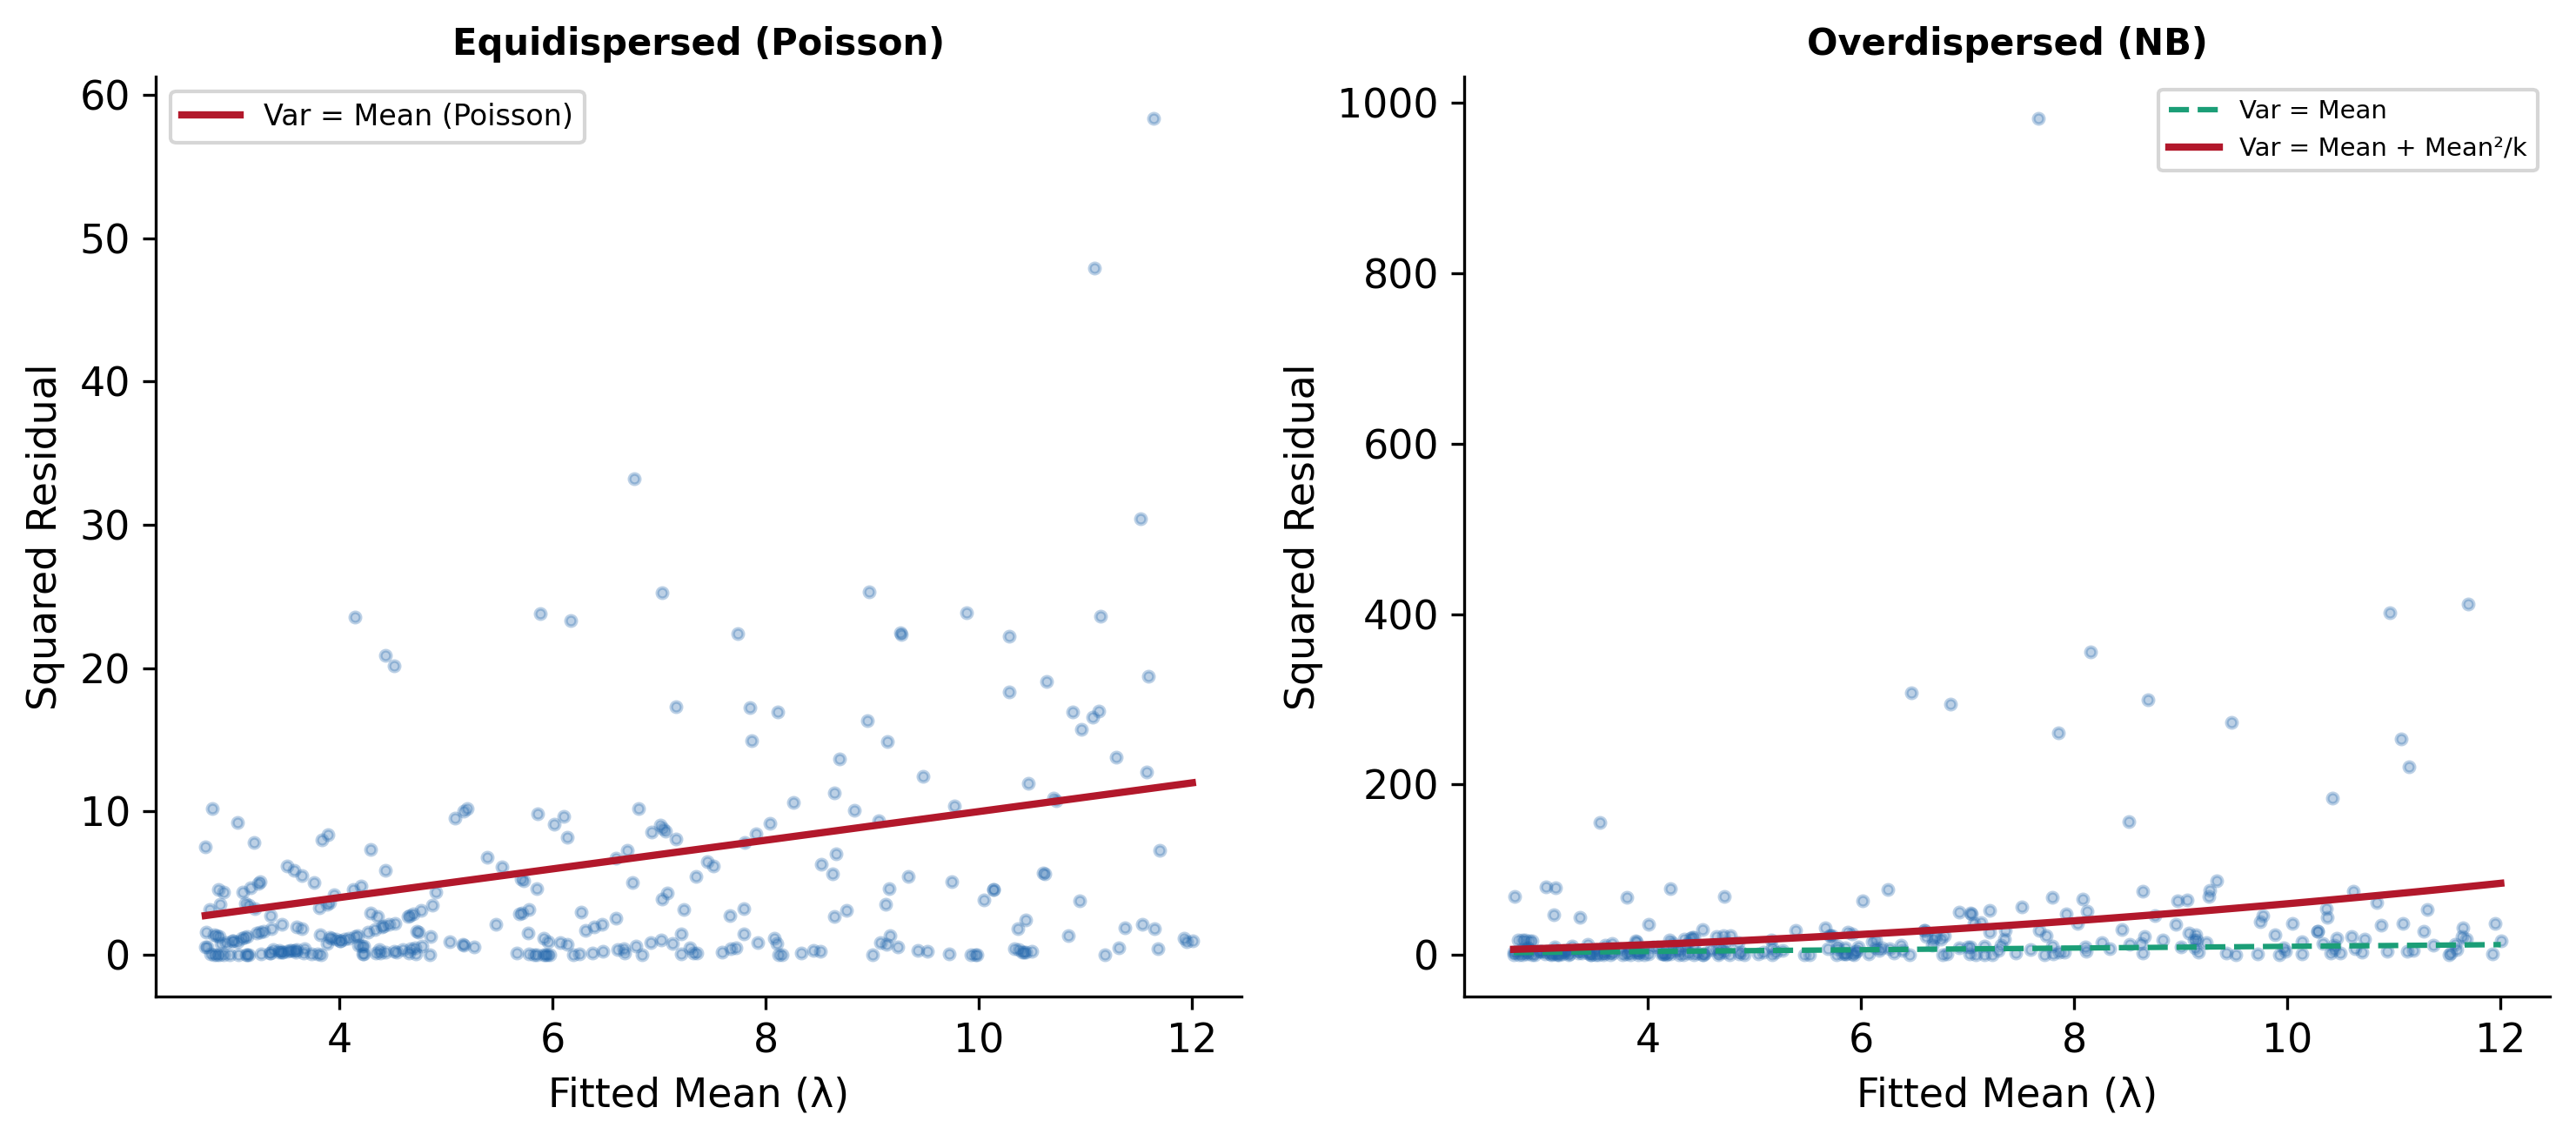
\includegraphics[width=0.85\textwidth]{m2_9_overdispersion.png}

\vspace{0.2cm}
\begin{columns}[T]
\begin{column}{0.48\textwidth}
\begin{itemize}
    \item Poisson: $\text{Var}(y) = \mu$ (strict)
    \item Overdispersion: $\text{Var}(y) > \mu$
    \item Causes: unmeasured heterogeneity, clustering, zero-inflation
    \item Dispersion parameter: $\hat{\phi} = \sum r^2_P / (n - p)$; if $\hat{\phi} \gg 1$, overdispersed
\end{itemize}
\end{column}
\begin{column}{0.48\textwidth}
\begin{alertblock}{Pro-Tip}
    \scriptsize Fixes: (1) quasi-Poisson (\texttt{family=quasipoisson}); (2) negative binomial (\texttt{MASS::glm.nb()}); (3) zero-inflated models (\texttt{pscl::zeroinfl()}). The DHARMa \texttt{testDispersion()} gives a formal test.
\end{alertblock}
\end{column}
\end{columns}
\end{frame}

% ── 253 ──
\begin{frame}[fragile]{Overdispersion --- Code}\smark{253/300}
\begin{columns}[T]
\begin{column}{0.48\textwidth}
\begin{lstlisting}[style=Rstyle]
# Check dispersion parameter
model_pois <- glm(count ~ x,
  family = poisson, data = df)
# Deviance / df.residual
summary(model_pois)$deviance /
  summary(model_pois)$df.residual
# If >> 1: overdispersed

# DHARMa formal test
testDispersion(simulateResiduals(
  model_pois))

# Fix: negative binomial
library(MASS)
model_nb <- glm.nb(count ~ x,
  data = df)
\end{lstlisting}
\end{column}
\begin{column}{0.48\textwidth}
\begin{lstlisting}[style=Pystyle]
# Dispersion parameter
phi = model.pearson_chi2 / model.df_resid
print(f"Dispersion: {phi:.2f}")

# If phi >> 1: overdispersed
# Fix: negative binomial
model_nb = sm.GLM(y, X,
    family=sm.families\
        .NegativeBinomial()
    ).fit()

# Or quasi-Poisson (manual)
# Scale SEs by sqrt(phi)
from statsmodels.genmod \
    .generalized_linear_model \
    import GLM
model_quasi = GLM(y, X,
    family=sm.families.Poisson()
    ).fit(scale="X2")
\end{lstlisting}
\end{column}
\end{columns}
\end{frame}

% ── 254 ──
\begin{frame}{Zero-Inflation Diagnostics}
\smark{254/300}
\begin{columns}[T]
\begin{column}{0.50\textwidth}
\begin{itemize}
    \item More zeros than the distribution predicts
    \item Observed zeros vs.\ expected zeros (Poisson/NB)
    \item \textbf{Rootogram}: hanging bars show observed $-$ expected per count value
    \item DHARMa: \texttt{testZeroInflation()} compares simulated vs.\ observed zero proportion
\end{itemize}
\end{column}
\begin{column}{0.47\textwidth}
\begin{alertblock}{Pro-Tip}
    \scriptsize R: \texttt{countreg::rootogram(model)} or \texttt{topmodels::rootogram()}. The ``hanging'' variant is best: bars hang from the expected line, and deviations from the baseline indicate misfit.
\end{alertblock}
\vspace{0.1cm}
\begin{exampleblock}{Data Insight}
    \scriptsize Fixes: zero-inflated Poisson (\texttt{pscl::zeroinfl()}), hurdle models (\texttt{pscl::hurdle()}), or zero-inflated negative binomial. Python: \texttt{statsmodels.ZeroInflatedPoisson}.
\end{exampleblock}
\end{column}
\end{columns}
\end{frame}

% ── 255 ──
\begin{frame}[fragile]{Zero-Inflation --- Code}\smark{255/300}
\begin{columns}[T]
\begin{column}{0.48\textwidth}
\begin{lstlisting}[style=Rstyle]
# Rootogram
library(topmodels)
rootogram(model_pois, style="hanging")

# Formal test (DHARMa)
testZeroInflation(sim_res)

# Fix: zero-inflated Poisson
library(pscl)
model_zip <- zeroinfl(count ~ x |1,
  data = df)

# Hurdle model
model_hurdle <- hurdle(count ~ x |1,
  data = df)
\end{lstlisting}
\end{column}
\begin{column}{0.48\textwidth}
\begin{lstlisting}[style=Pystyle]
# Compare observed vs expected zeros
obs_zeros = np.sum(y == 0)
exp_zeros = np.sum(
    stats.poisson.pmf(0, model.mu))
print(f"Obs: {obs_zeros}, "
      f"Exp: {exp_zeros:.1f}")

# Zero-inflated Poisson
from statsmodels.discrete \
    .count_model import \
    ZeroInflatedPoisson
model_zip = ZeroInflatedPoisson(
    y, X, exog_infl=X).fit()

# Rootogram: manual bar chart
# of observed vs expected counts
\end{lstlisting}
\end{column}
\end{columns}
\end{frame}

% ── 256 ──
\begin{frame}{Mixed Models: Caterpillar Plots}
\smark{256/300}
\centering
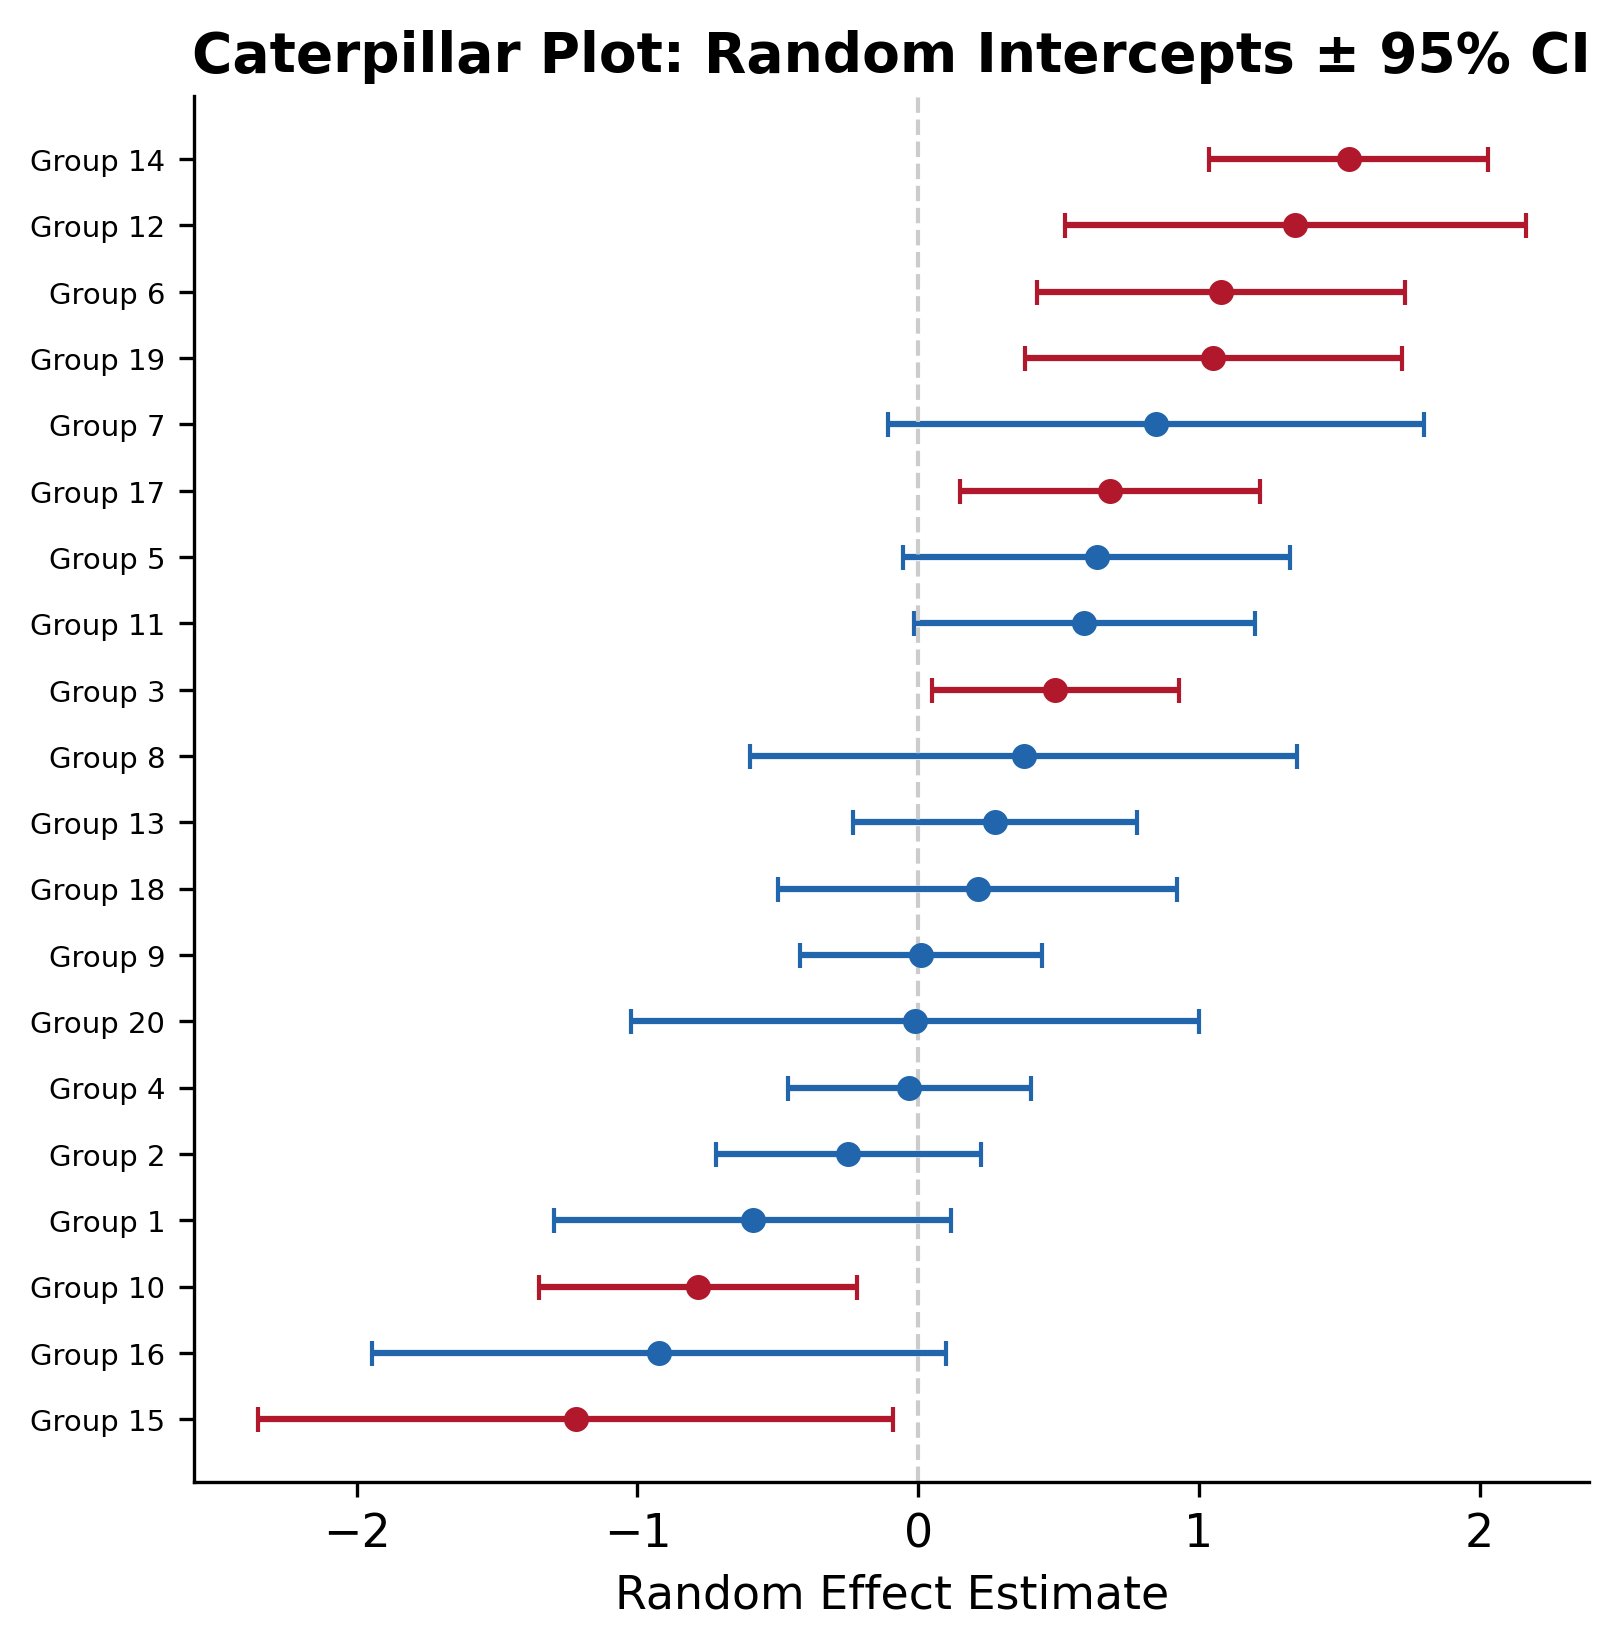
\includegraphics[width=0.55\textwidth]{m2_9_caterpillar.png}

\vspace{0.2cm}
\begin{columns}[T]
\begin{column}{0.48\textwidth}
\begin{itemize}
    \item Random effect estimates sorted by value
    \item Horizontal CI per group
    \item Red = CI excludes zero (group significantly deviates from the grand mean)
    \item Blue = CI includes zero
    \item Named for the ``fuzzy caterpillar'' shape
\end{itemize}
\end{column}
\begin{column}{0.48\textwidth}
\begin{exampleblock}{Data Insight}
    \scriptsize The caterpillar plot is the primary diagnostic for random intercepts. It shows (1) how much groups vary, (2) which groups are outliers, and (3) whether the random-effect variance is well-estimated.
\end{exampleblock}
\end{column}
\end{columns}
\end{frame}

% ── 257 ──
\begin{frame}[fragile]{Caterpillar Plot --- Code}\smark{257/300}
\begin{columns}[T]
\begin{column}{0.48\textwidth}
\begin{lstlisting}[style=Rstyle]
library(lme4)

model <- lmer(body_mass_g ~
  bill_length_mm +
  (1 | species/island),
  data = penguins)

# Caterpillar plot
library(lattice)
dotplot(ranef(model,
  condVar = TRUE))

# ggplot2 approach
re <- ranef(model, condVar=TRUE)
df_re <- as.data.frame(re)
ggplot(df_re, aes(condval,
    fct_reorder(grp, condval))) +
  geom_pointrange(
    aes(xmin=condval-1.96*condsd,
        xmax=condval+1.96*condsd)) +
  geom_vline(xintercept=0,
    linetype="dashed")
\end{lstlisting}
\end{column}
\begin{column}{0.48\textwidth}
\begin{lstlisting}[style=Pystyle]
import statsmodels.formula.api as smf

model = smf.mixedlm(
    "body_mass_g ~ bill_length_mm",
    data=penguins,
    groups=penguins["species"]).fit()

# Extract random effects
re = model.random_effects
re_df = pd.DataFrame({
    "group": re.keys(),
    "intercept": [v["Group"]
        for v in re.values()]})

# Manual caterpillar
ax.errorbar(re_df["intercept"],
    range(len(re_df)),
    xerr=1.96*se_estimates,
    fmt="o", capsize=3)
ax.axvline(0, linestyle="--")
\end{lstlisting}
\end{column}
\end{columns}
\end{frame}

% ── 258 ──
\begin{frame}{QQ Plot of Random Effects}
\smark{258/300}
\centering
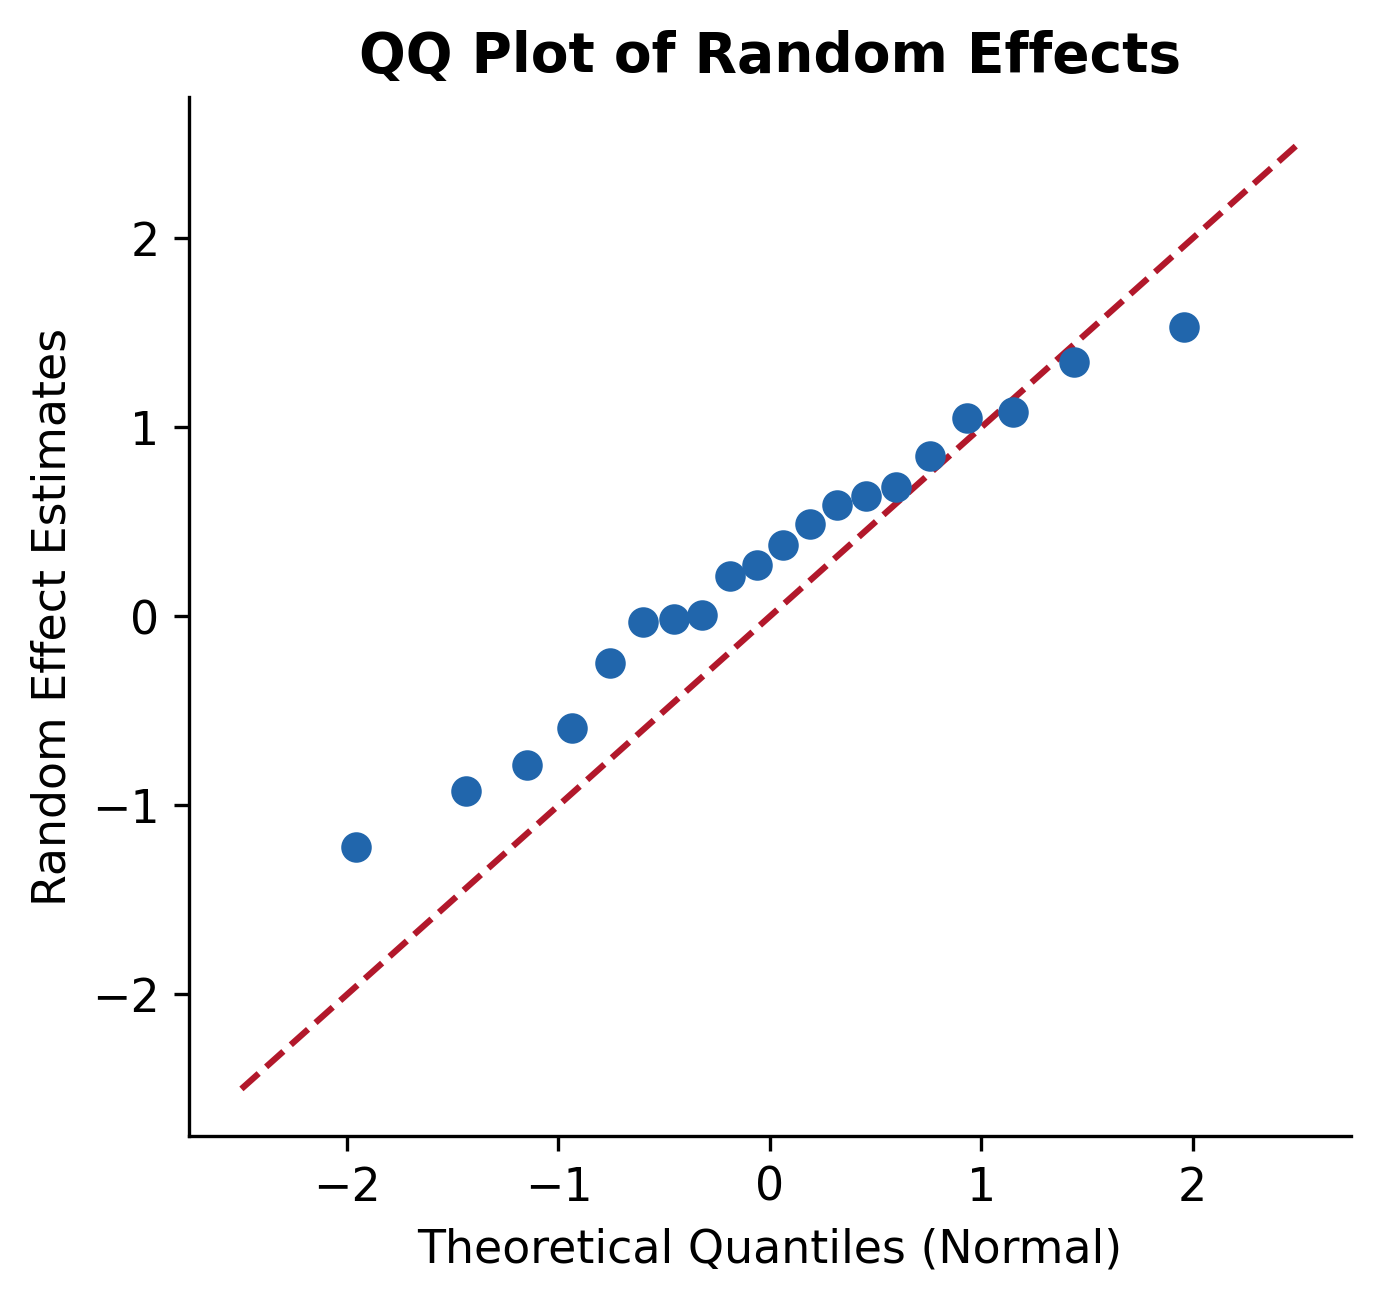
\includegraphics[width=0.52\textwidth]{m2_9_re_qq.png}

\vspace{0.2cm}
\begin{columns}[T]
\begin{column}{0.48\textwidth}
\begin{itemize}
    \item Random effects are assumed $\sim N(0, \sigma^2_u)$
    \item QQ plot checks this assumption
    \item Deviations from the line $\to$ non-normal grouping structure
    \item Heavy tails $\to$ outlier groups pulling the model
\end{itemize}
\end{column}
\begin{column}{0.48\textwidth}
\begin{alertblock}{Pro-Tip}
    \scriptsize With few groups ($< 10$), the QQ plot has too few points to be reliable. The normality assumption matters most when making predictions for new groups. With many groups ($> 30$), mild non-normality is tolerable.
\end{alertblock}
\end{column}
\end{columns}
\end{frame}

% ── 259 ──
\begin{frame}[fragile]{RE QQ Plot --- Code}\smark{259/300}
\begin{columns}[T]
\begin{column}{0.48\textwidth}
\begin{lstlisting}[style=Rstyle]
# Extract BLUPs
re_vals <- ranef(model)$group[,1]

# QQ plot
qqnorm(re_vals, pch=19,
  col="#2166AC")
qqline(re_vals, col="#B2182B",
  lwd=2)

# ggplot2
ggplot(data.frame(re=re_vals),
  aes(sample=re)) +
  geom_qq(color="#2166AC") +
  geom_qq_line(color="#B2182B") +
  theme_minimal()
\end{lstlisting}
\end{column}
\begin{column}{0.48\textwidth}
\begin{lstlisting}[style=Pystyle]
re_vals = np.array([
    v["Group"]
    for v in model.random_effects
        .values()])

# scipy QQ
fig, ax = plt.subplots()
stats.probplot(re_vals,
    dist="norm", plot=ax)

# manual
sorted_re = np.sort(re_vals)
theoretical = stats.norm.ppf(
    np.linspace(0.025, 0.975,
                len(sorted_re)))
ax.scatter(theoretical, sorted_re)
ax.plot([-3,3],[-3,3],"--",
    color="#B2182B")
\end{lstlisting}
\end{column}
\end{columns}
\end{frame}

% ── 260 ──
\begin{frame}{Residuals by Group: Heterogeneous Variance}
\smark{260/300}
\centering
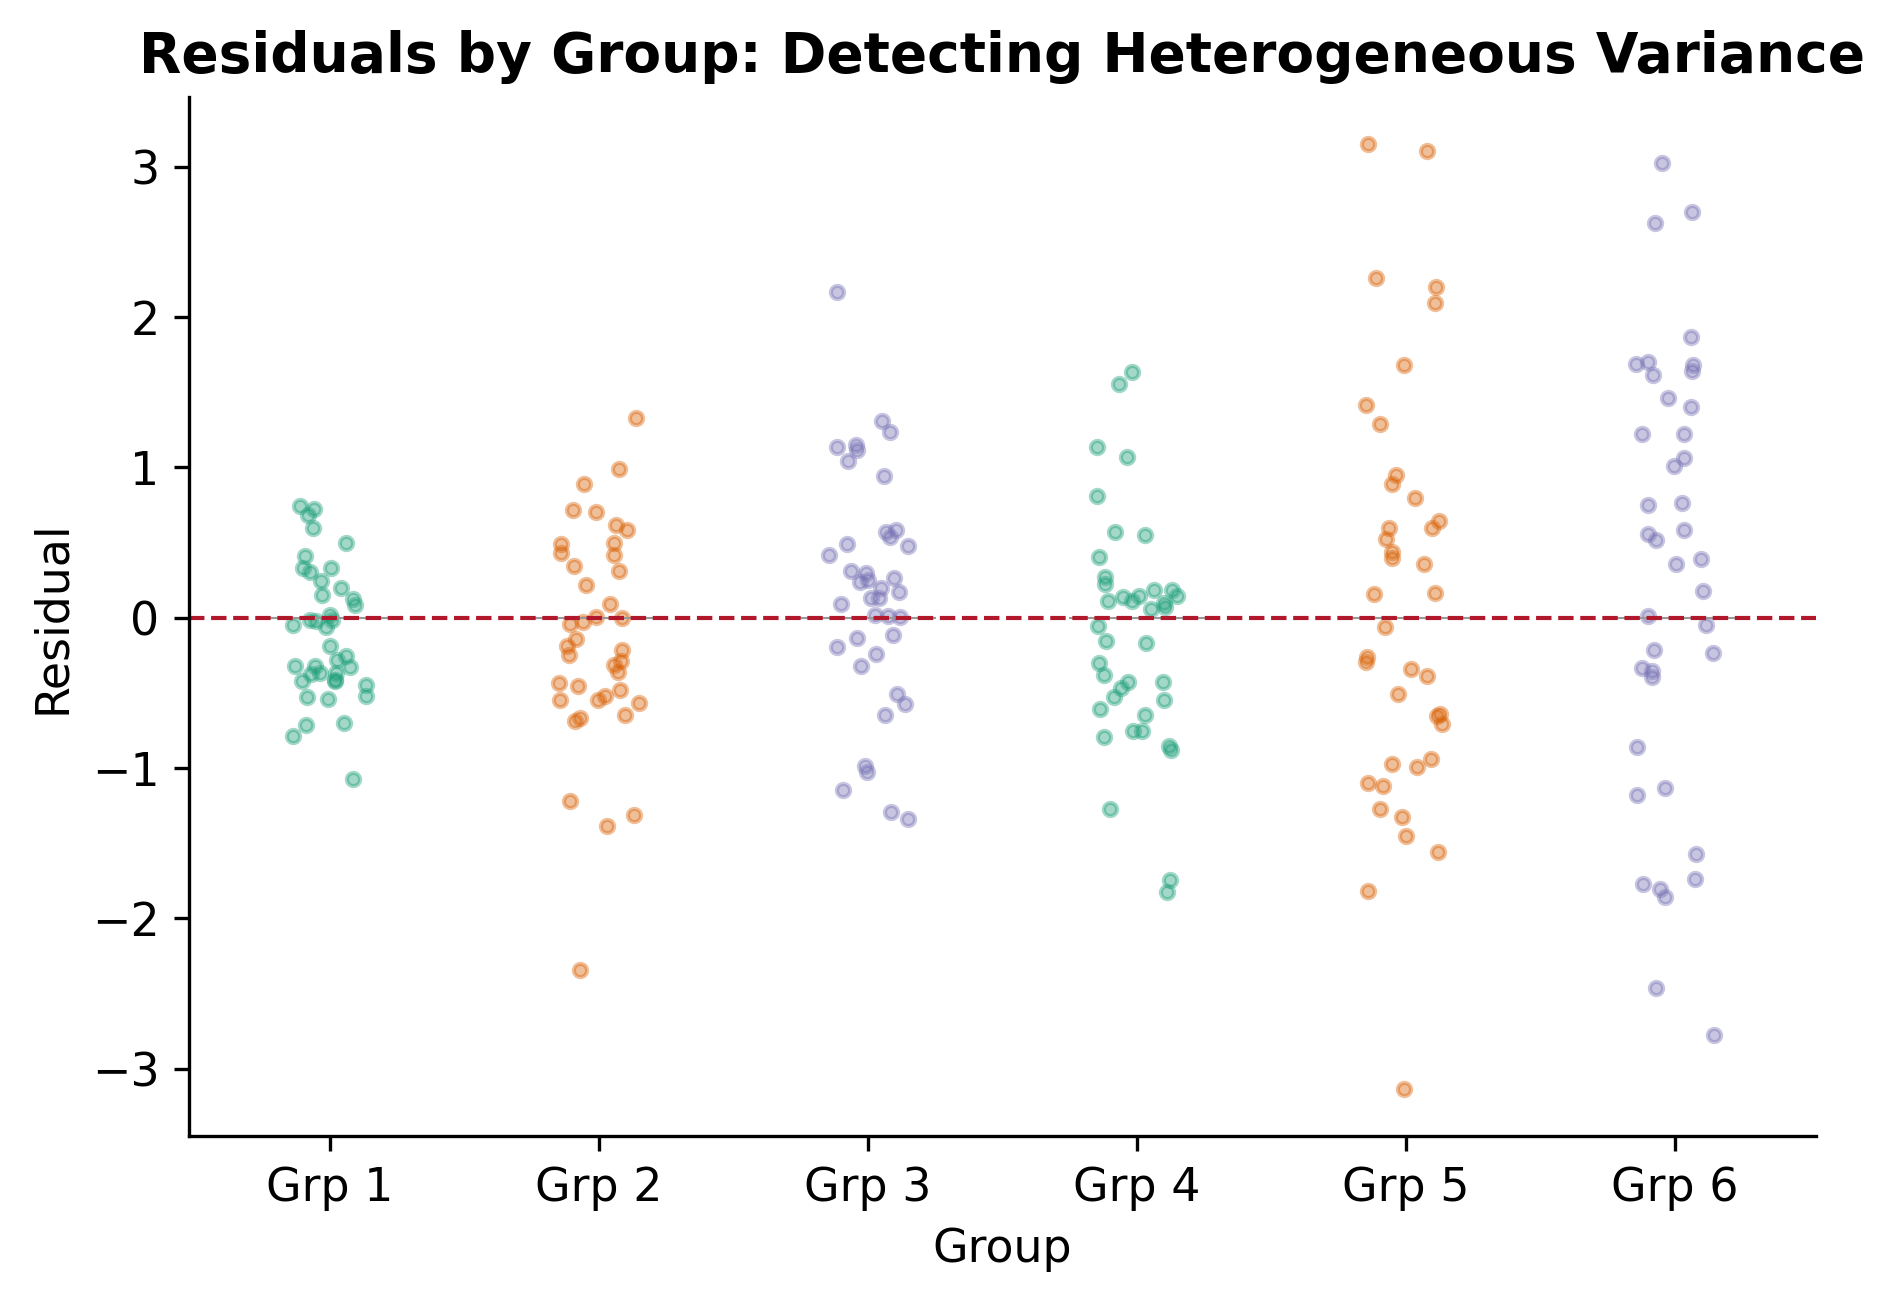
\includegraphics[width=0.72\textwidth]{m2_9_resid_by_group.png}

\vspace{0.2cm}
\begin{columns}[T]
\begin{column}{0.48\textwidth}
\begin{itemize}
    \item Plot level-1 residuals faceted or colored by group
    \item If spread differs across groups $\to$ heterogeneous within-group variance
    \item Violates the standard mixed-model assumption
    \item Fix: model heterogeneous variance with \texttt{nlme::lme(weights=varIdent())}
\end{itemize}
\end{column}
\begin{column}{0.48\textwidth}
\begin{alertblock}{Pro-Tip}
    \scriptsize \texttt{lme4::lmer()} cannot model heterogeneous variance directly. Use \texttt{nlme::lme()} with \texttt{weights=varIdent(form=\textasciitilde1|group)} or \texttt{glmmTMB} with the \texttt{dispformula} argument.
\end{alertblock}
\end{column}
\end{columns}
\end{frame}

% ── 261 ──
\begin{frame}[fragile]{Residuals by Group --- Code}\smark{261/300}
\begin{columns}[T]
\begin{column}{0.48\textwidth}
\begin{lstlisting}[style=Rstyle]
# Extract residuals
df$resid <- residuals(model)

# Strip plot by group
ggplot(df, aes(group, resid)) +
  geom_jitter(width=0.15,
    alpha=0.3, size=1) +
  geom_hline(yintercept=0,
    linetype="dashed",
    color="#B2182B") +
  theme_minimal()

# Fix: heterogeneous variance
library(nlme)
model_het <- lme(y ~ x,
  random = ~1|group,
  weights = varIdent(
    form = ~1|group),
  data = df)
\end{lstlisting}
\end{column}
\begin{column}{0.48\textwidth}
\begin{lstlisting}[style=Pystyle]
# Residuals by group
resid = model.resid
groups = penguins["species"]

fig, ax = plt.subplots()
for i, grp in enumerate(
    groups.unique()):
    mask = groups == grp
    r = resid[mask]
    jitter = np.random.uniform(
        -0.15, 0.15, len(r))
    ax.scatter(
        np.full(len(r), i)+jitter,
        r, s=10, alpha=0.3)
ax.axhline(0, linestyle="--",
    color="#B2182B")
ax.set_xticks(range(len(
    groups.unique())))
ax.set_xticklabels(groups.unique())
\end{lstlisting}
\end{column}
\end{columns}
\end{frame}

% ── 262 ──
\begin{frame}{Mixed-Model Diagnostic Checklist}
\smark{262/300}
\centering\small
\begin{tabular}{@{}lll@{}}
    \toprule
    \textbf{Assumption} & \textbf{Plot} & \textbf{R Tool} \\
    \midrule
    Linearity              & Residuals vs.\ fitted         & \texttt{plot(model)} \\
    Normality of residuals & QQ of level-1 residuals       & \texttt{qqnorm(resid())} \\
    Normality of RE        & QQ of random effects           & \texttt{qqnorm(ranef())} \\
    Homoscedasticity       & Residuals by group / fitted    & \texttt{plot(model)} \\
    Independence           & Residuals vs.\ time / order    & \texttt{acf(resid())} \\
    Influential groups     & Cook's $D$ per group           & \texttt{influence.ME} \\
    RE magnitude           & Caterpillar plot               & \texttt{dotplot(ranef())} \\
    \bottomrule
\end{tabular}

\vspace{0.3cm}
\begin{exampleblock}{Data Insight}
    \scriptsize The \texttt{performance::check\_model()} function works for \texttt{lmer()} objects and produces all panels automatically. DHARMa also supports mixed models via \texttt{simulateResiduals(lmer\_model)}.
\end{exampleblock}
\end{frame}

% ── 263 ──
\begin{frame}{DHARMa for Mixed Models and Beyond}
\smark{263/300}
\begin{columns}[T]
\begin{column}{0.50\textwidth}
\begin{itemize}
    \item DHARMa works for \textbf{any} model with a \texttt{simulate()} method
    \item Supported: \texttt{glm}, \texttt{lmer}, \texttt{glmer}, \texttt{glmmTMB}, \texttt{brms}, \texttt{mgcv::gam}
    \item Standard interface: \texttt{simulateResiduals()} + \texttt{plot()}
    \item Formal tests: dispersion, zero-inflation, outliers, uniformity
\end{itemize}
\end{column}
\begin{column}{0.47\textwidth}
\begin{alertblock}{Pro-Tip}
    \scriptsize DHARMa (Hartig, 2022) is the single most useful diagnostic package for non-Gaussian models. Install it for any project involving GLMs, GLMMs, or GAMs. The \texttt{plot()} output gives you the complete diagnostic in two panels.
\end{alertblock}
\end{column}
\end{columns}
\end{frame}

% ── 264 ──
\begin{frame}[fragile]{DHARMa for Mixed Models --- Code}\smark{264/300}
\begin{columns}[T]
\begin{column}{0.48\textwidth}
\begin{lstlisting}[style=Rstyle]
library(lme4)
library(DHARMa)

# Poisson GLMM
model <- glmer(count ~
  treatment + (1|site),
  family = poisson, data = df)

# Simulate residuals
sim_res <- simulateResiduals(
  fittedModel = model,
  n = 1000)

# Standard panel
plot(sim_res)

# Per-group diagnostics
plotResiduals(sim_res,
  form = df$site)
\end{lstlisting}
\end{column}
\begin{column}{0.48\textwidth}
\begin{lstlisting}[style=Pystyle]
# Python: no DHARMa equivalent.
# Manual simulation approach:

# 1. Fit model
# 2. Simulate n_sim datasets
# 3. Compute quantile residuals
# 4. QQ against uniform

# For mixed models in Python:
# statsmodels.MixedLM (LMM only)
# Use R via rpy2 for GLMMs:
from rpy2.robjects.packages \
    import importr
dharma = importr("DHARMa")
# Call DHARMa functions via rpy2
\end{lstlisting}
\vspace{0.1cm}
\begin{exampleblock}{Data Insight}
    \scriptsize For GLMMs in Python, the ecosystem is limited. \texttt{rpy2} bridges to R's DHARMa/lme4 when needed. Native Python GLMM support is growing via \texttt{bambi} (Bayesian).
\end{exampleblock}
\end{column}
\end{columns}
\end{frame}

% ── 265 ──
\begin{frame}{Influence Diagnostics for Mixed Models}
\smark{265/300}
\begin{columns}[T]
\begin{column}{0.50\textwidth}
\begin{itemize}
    \item \textbf{Observation-level}: outlier within a group
    \item \textbf{Group-level}: an entire group distorts the fixed effects
    \item Cook's $D$ at group level: refit the model dropping each group, measure $\hat{\beta}$ change
    \item \texttt{influence.ME} package automates this
\end{itemize}
\end{column}
\begin{column}{0.47\textwidth}
\begin{alertblock}{Pro-Tip}
    \scriptsize R: \texttt{influence.ME::influence(model, group="site")} then \texttt{cooks.distance()} at the group level. Computationally expensive for many groups but essential for checking robustness.
\end{alertblock}
\vspace{0.1cm}
\begin{exampleblock}{Data Insight}
    \scriptsize If dropping one group changes $\hat{\beta}$ by $> 20\%$, that group is driving the result. Report sensitivity: ``Results hold when Group X is excluded.''
\end{exampleblock}
\end{column}
\end{columns}
\end{frame}

% ── 266 ──
\begin{frame}[fragile]{Group-Level Influence --- Code}\smark{266/300}
\begin{columns}[T]
\begin{column}{0.48\textwidth}
\begin{lstlisting}[style=Rstyle]
library(influence.ME)

model <- lmer(y ~ x + (1|group),
              data = df)

# Group-level influence
infl <- influence(model,
                  group = "group")

# Cook's D per group
cooks.distance(infl)

# DFBETAS per group
dfbetas(infl)

# Plot
plot(infl, which = "cook",
     sort = TRUE)
\end{lstlisting}
\end{column}
\begin{column}{0.48\textwidth}
\begin{lstlisting}[style=Pystyle]
# Manual leave-one-group-out
groups = df["group"].unique()
betas = {}
for g in groups:
    df_sub = df[df["group"] != g]
    m_sub = smf.mixedlm(
        "y ~ x", data=df_sub,
        groups=df_sub["group"]).fit()
    betas[g] = m_sub.params["x"]

# Compare to full model
full_beta = model.params["x"]
cook_approx = {g: (b-full_beta)**2
    for g, b in betas.items()}

# Bar plot of influence
ax.barh(list(cook_approx.keys()),
    list(cook_approx.values()))
\end{lstlisting}
\end{column}
\end{columns}
\end{frame}

% ── 267 ──
\begin{frame}{ICC: Intraclass Correlation Coefficient}
\smark{267/300}
\begin{columns}[T]
\begin{column}{0.50\textwidth}
\begin{itemize}
    \item $\text{ICC} = \sigma^2_u / (\sigma^2_u + \sigma^2_e)$
    \item Proportion of total variance explained by the grouping
    \item ICC $\approx$ 0: groups don't matter (ignore clustering)
    \item ICC $\approx$ 1: all variance is between groups
    \item Visualize with caterpillar plot width or a variance decomposition bar
\end{itemize}
\end{column}
\begin{column}{0.47\textwidth}
\begin{alertblock}{Pro-Tip}
    \scriptsize R: \texttt{performance::icc(model)}. Python: manual from \texttt{model.cov\_re} and \texttt{model.scale}. If ICC $< 0.05$, a mixed model may be unnecessary --- but report it anyway.
\end{alertblock}
\vspace{0.1cm}
\begin{exampleblock}{Data Insight}
    \scriptsize A visual alternative to the numeric ICC: a stacked bar showing $\sigma^2_u$ and $\sigma^2_e$ as proportions. Multiple random effects produce a multi-segment bar.
\end{exampleblock}
\end{column}
\end{columns}
\end{frame}

% ── 268 ──
\begin{frame}{GLM / Mixed-Model Diagnostic Decision Guide}
\smark{268/300}
\centering\small
\begin{tabular}{@{}llll@{}}
    \toprule
    \textbf{Model} & \textbf{Key Diagnostic} & \textbf{R Package} & \textbf{Python} \\
    \midrule
    Logistic GLM     & Binned residuals, ROC    & \texttt{arm}, \texttt{pROC}      & Manual, sklearn \\
    Poisson GLM      & Overdispersion, rootogram & \texttt{DHARMa}               & Manual \\
    Negative binomial& DHARMa QQ                 & \texttt{DHARMa}               & Manual \\
    Zero-inflated    & Zero proportion test       & \texttt{DHARMa}, \texttt{pscl} & \texttt{statsmodels} \\
    LMM (\texttt{lmer}) & Caterpillar, RE QQ     & \texttt{lme4}, \texttt{performance} & \texttt{statsmodels} \\
    GLMM             & DHARMa simulation          & \texttt{DHARMa}, \texttt{glmmTMB}  & \texttt{rpy2} bridge \\
    GAM              & \texttt{gam.check()}       & \texttt{mgcv}                  & \texttt{pygam} \\
    \bottomrule
\end{tabular}
\end{frame}

% ── 269 ──
\begin{frame}{The \texttt{performance} Package: One-Stop Diagnostics}
\smark{269/300}
\begin{columns}[T]
\begin{column}{0.50\textwidth}
\begin{itemize}
    \item \texttt{check\_model()}: auto-detects model class and produces appropriate panels
    \item Works for \texttt{lm}, \texttt{glm}, \texttt{lmer}, \texttt{glmer}
    \item Includes: residual QQ, homogeneity, influential points, collinearity (VIF), normality of RE, posterior predictive check
    \item One function call, 6+ panels
\end{itemize}
\end{column}
\begin{column}{0.47\textwidth}
\begin{alertblock}{Pro-Tip}
    \scriptsize \texttt{performance::check\_model(model)} is the \textbf{single best diagnostic command} in R. It replaces 6 separate plot calls. For Python, the closest equivalent is manually combining \texttt{statsmodels.graphics} panels.
\end{alertblock}
\end{column}
\end{columns}
\end{frame}

% ── 270 ──
\begin{frame}{Module 2.9 --- Key Takeaways}\smark{270/300}
\begin{enumerate}
    \item \textbf{OLS residuals fail for GLMs.} Use Pearson, deviance, or quantile residuals.
    \item \textbf{DHARMa} provides universal diagnostics via simulation --- works for any model.
    \item \textbf{Binned residual plots} are the correct diagnostic for logistic regression.
    \item \textbf{Overdispersion}: check dispersion parameter; fix with quasi-Poisson or NB.
    \item \textbf{Caterpillar plots} diagnose random effects; QQ checks their normality.
    \item \textbf{Residuals by group} detect heterogeneous within-group variance.
\end{enumerate}
\end{frame}

% ── 271 ──
\begin{frame}{}\smark{271/300}
\centering\vspace{1.5cm}
{\Large\textbf{Module 2.9 Complete}}\\[0.5cm]
You can now diagnose GLMs (logistic, Poisson, NB, zero-inflated) and mixed models (LMM, GLMM) with appropriate residuals, simulation-based tests, caterpillar plots, and group-level influence checks.\\[0.5cm]
\textbf{Next:} Module 2.10 --- Workshop Summary and Comprehensive Reference.
\end{frame}

% % ═══════════════════════════════════════════════════════
%  MODULE 2.10 — Workshop Summary and Comprehensive Reference
% ═══════════════════════════════════════════════════════
\section{Module 2.10 --- Workshop Summary and Reference}

% ── 272 ──
\begin{frame}{Module 2.10 --- Workshop 2 Recap}\smark{272/300}
\begin{enumerate}
    \item Module 2.1 --- Summary Statistics: dynamite plots, strip, bootstrap CI
    \item Module 2.2 --- Boxplots, Violins, Raincloud, Beeswarm
    \item Module 2.3 --- Regression Diagnostics and Model Visualization
    \item Module 2.4 --- Uncertainty Visualization
    \item Module 2.5 --- Interactions, Marginal Means, Effect Plots
    \item Module 2.6 --- Correlation, Association, Heatmaps
    \item Module 2.7 --- Hypothesis Tests and $p$-Value Displays
    \item Module 2.8 --- Classification Diagnostics
    \item Module 2.9 --- GLM and Mixed-Model Residuals
    \item Module 2.10 --- This summary
\end{enumerate}
\end{frame}

% ── 273 ──
\begin{frame}{The Statistical Visualization Hierarchy}
\smark{273/300}
\centering\small
\begin{tabular}{@{}lll@{}}
    \toprule
    \textbf{Level} & \textbf{What You Show} & \textbf{Key Plots} \\
    \midrule
    1. Raw data        & Every observation          & Strip, jitter, beeswarm \\
    2. Distribution    & Shape, center, spread      & Violin, raincloud, ridgeline \\
    3. Summary         & Point estimate $\pm$ CI    & Pointrange, slab+interval \\
    4. Model fit       & Predicted values + band    & Effect plot, coefficient plot \\
    5. Diagnostics     & Residuals, QQ, influence   & 4-panel, DHARMa, Cook's $D$ \\
    6. Inference       & Effect size, difference CI & Estimation plot, forest plot \\
    7. Classification  & Discrimination, calibration& ROC, PR, calibration, gain \\
    \bottomrule
\end{tabular}

\vspace{0.3cm}
\begin{exampleblock}{Data Insight}
    \scriptsize Workshop 2 covered levels 1--7. Workshop 1 covered levels 1--3 (foundations). Each level adds one layer of statistical sophistication to the visualization.
\end{exampleblock}
\end{frame}

% ── 274 ──
\begin{frame}{The ``Show Your Data'' Manifesto}
\smark{274/300}
\begin{columns}[T]
\begin{column}{0.50\textwidth}
\begin{enumerate}
    \item \textbf{Show raw data} when $n$ permits (strip, jitter, beeswarm)
    \item \textbf{Show the distribution} when $n$ is large (violin, raincloud)
    \item \textbf{Show uncertainty} always (CI, PI, slab+interval, gradient)
    \item \textbf{Show the effect size}, not just significance
    \item \textbf{Show the model}, not just the summary table
    \item \textbf{Show the diagnostics}, not just $R^2$
\end{enumerate}
\end{column}
\begin{column}{0.47\textwidth}
\begin{alertblock}{Pro-Tip}
    \scriptsize Each ``show'' replaces a number in a table with a visual that reveals more: shape, outliers, precision, direction, magnitude, and model fit. Tables compress; visualizations expand.
\end{alertblock}
\end{column}
\end{columns}
\end{frame}

% ── 275 ──
\begin{frame}{Distribution Plot Decision Matrix}
\smark{275/300}
\centering\small
\begin{tabular}{@{}llll@{}}
    \toprule
    \textbf{$n$ per group} & \textbf{Groups} & \textbf{Goal} & \textbf{Best Plot} \\
    \midrule
    $< 10$        & 2--5    & Show every point        & Strip only \\
    $10$--$50$    & 2--5    & Shape + raw data        & Raincloud or hybrid \\
    $50$--$200$   & 2--5    & Shape + summary         & Violin + box \\
    $> 200$       & 2--5    & Shape only              & Violin or letter-value \\
    Any           & 2--5    & Quick inference         & Notched boxplot \\
    Any           & 5--30   & Compare many groups     & Ridgeline \\
    $20$--$200$   & 2--5    & Non-overlapping points  & Beeswarm \\
    \bottomrule
\end{tabular}
\end{frame}

% ── 276 ──
\begin{frame}{Uncertainty Visualization Decision Matrix}
\smark{276/300}
\centering\small
\begin{tabular}{@{}lll@{}}
    \toprule
    \textbf{Audience} & \textbf{Context} & \textbf{Best Representation} \\
    \midrule
    Statisticians        & Paper / review      & Slab + interval (ggdist) \\
    Scientists           & Talk / poster       & Pointrange or gradient \\
    Decision-makers      & Dashboard           & Fan chart or gradient \\
    General public       & News / infographic  & HOPs or quantile dots \\
    Meta-analysis        & Systematic review   & Forest plot \\
    Bayesian             & Posterior reporting  & HDI + density \\
    Time series          & Forecast            & Ribbon or fan chart \\
    \bottomrule
\end{tabular}
\end{frame}

% ── 277 ──
\begin{frame}{Regression Diagnostic Flowchart}
\smark{277/300}
\centering\small
\begin{tabular}{@{}llll@{}}
    \toprule
    \textbf{Pattern} & \textbf{Problem} & \textbf{Fix} & \textbf{Plot} \\
    \midrule
    Curve in residuals       & Non-linearity     & Polynomial / GAM        & Resid vs.\ Fitted \\
    Funnel in residuals      & Heteroscedasticity& Log $y$ / WLS / robust  & Scale-Location \\
    Heavy tails on QQ        & Non-normality     & Bootstrap CIs           & Normal QQ \\
    High Cook's $D$          & Influential point & Investigate              & Cook's stem plot \\
    Non-parallel lines       & Interaction       & Add interaction term     & Grouped regression \\
    Pooled reversal          & Simpson's paradox & Include confounder       & Color by group \\
    \bottomrule
\end{tabular}
\end{frame}

% ── 278 ──
\begin{frame}{Classification Diagnostic Workflow}
\smark{278/300}
\centering\small
\begin{tabular}{@{}ll@{}}
    \toprule
    \textbf{Step} & \textbf{Plot} \\
    \midrule
    1. Score separation      & Score distributions by class \\
    2. Discrimination        & ROC (balanced) / PR (imbalanced) \\
    3. Calibration           & Reliability diagram + Brier \\
    4. Threshold             & Metrics-vs-threshold \\
    5. Error profile         & Confusion matrix \\
    6. Business translation  & Gain / lift \\
    7. Clinical decision     & Decision curve analysis \\
    \bottomrule
\end{tabular}

\vspace{0.3cm}
\begin{alertblock}{Pro-Tip}
    \scriptsize This 7-step workflow applies to \textbf{any} binary classifier: logistic regression, random forest, XGBoost, neural network. The plots are model-agnostic --- only the predicted scores matter.
\end{alertblock}
\end{frame}

% ── 279 ──
\begin{frame}{GLM and Mixed-Model Diagnostic Guide}
\smark{279/300}
\centering\small
\begin{tabular}{@{}llll@{}}
    \toprule
    \textbf{Model} & \textbf{Key Diagnostic} & \textbf{R} & \textbf{Python} \\
    \midrule
    Logistic         & Binned residuals, ROC    & \texttt{arm}, \texttt{pROC}      & Manual, sklearn \\
    Poisson          & Overdispersion, rootogram & \texttt{DHARMa}               & Manual \\
    Neg.\ Binomial   & DHARMa QQ                & \texttt{DHARMa}               & Manual \\
    Zero-inflated    & Zero proportion test      & \texttt{DHARMa}, \texttt{pscl} & \texttt{statsmodels} \\
    LMM              & Caterpillar, RE QQ        & \texttt{lme4}                 & \texttt{statsmodels} \\
    GLMM             & DHARMa simulation         & \texttt{glmmTMB}              & \texttt{rpy2} bridge \\
    \bottomrule
\end{tabular}
\end{frame}

% ── 280 ──
\begin{frame}{The Estimation Statistics Paradigm}
\smark{280/300}
\centering\small
\begin{tabular}{@{}lll@{}}
    \toprule
    \textbf{Old} & \textbf{New} & \textbf{Tool} \\
    \midrule
    Bar + stars only          & Strip + effect size CI     & \texttt{dabestr} \\
    $p$-value (binary)        & Effect size + CI           & \texttt{effectsize} \\
    Star brackets             & Difference CI              & Gardner--Altman \\
    ``Significant''           & ``$\Delta = 1387 \pm 118$\,g'' & Estimation plot \\
    NHST table                & Visual summary             & \texttt{ggdist}, \texttt{dabestr} \\
    \bottomrule
\end{tabular}

\vspace{0.3cm}
\begin{exampleblock}{Data Insight}
    \scriptsize Endorsed by: APA (7th ed.), Nature Methods, eLife, ASA Statement on $p$-values (2016). The shift is not optional --- it is the trajectory of statistical practice.
\end{exampleblock}
\end{frame}

% ── 281 ──
\begin{frame}{Master Package Reference --- \Rlang}
\smark{281/300}
\centering\scriptsize
\begin{tabular}{@{}lll@{}}
    \toprule
    \textbf{Task} & \textbf{Package} & \textbf{Key Function} \\
    \midrule
    Grammar of graphics  & \texttt{ggplot2}        & \texttt{ggplot() + geom\_*()} \\
    Distribution display & \texttt{ggdist}         & \texttt{stat\_halfeye()}, \texttt{stat\_dots()} \\
    Raincloud            & \texttt{ggdist}, \texttt{ggrain}& \texttt{stat\_halfeye()}, \texttt{geom\_rain()} \\
    Beeswarm             & \texttt{ggbeeswarm}     & \texttt{geom\_beeswarm()}, \texttt{geom\_sina()} \\
    Ridgeline            & \texttt{ggridges}       & \texttt{geom\_density\_ridges()} \\
    Estimation stats     & \texttt{dabestr}        & \texttt{dabest() |> mean\_diff() |> plot()} \\
    Marginal means       & \texttt{emmeans}        & \texttt{emmeans()}, \texttt{pairs()} \\
    Marginal effects     & \texttt{marginaleffects}& \texttt{plot\_predictions()}, \texttt{slopes()} \\
    Effect size          & \texttt{effectsize}     & \texttt{cohens\_d()}, \texttt{eta\_squared()} \\
    Model diagnostics    & \texttt{performance}    & \texttt{check\_model()} \\
    GLM diagnostics      & \texttt{DHARMa}         & \texttt{simulateResiduals()} \\
    Correlation          & \texttt{ggcorrplot}     & \texttt{ggcorrplot()} \\
    ROC / AUC            & \texttt{pROC}           & \texttt{roc()}, \texttt{ggroc()} \\
    Power analysis       & \texttt{pwr}            & \texttt{pwr.t.test()} \\
    Significance brackets& \texttt{ggpubr}         & \texttt{stat\_compare\_means()} \\
    \bottomrule
\end{tabular}
\end{frame}

% ── 282 ──
\begin{frame}{Master Package Reference --- \Python}
\smark{282/300}
\centering\scriptsize
\begin{tabular}{@{}lll@{}}
    \toprule
    \textbf{Task} & \textbf{Package} & \textbf{Key Function} \\
    \midrule
    Grammar of graphics  & \texttt{plotnine}       & \texttt{ggplot() + geom\_*()} \\
    Statistical plots     & \texttt{seaborn}        & \texttt{violinplot}, \texttt{pointplot} \\
    Estimation stats     & \texttt{dabest}         & \texttt{load() .mean\_diff.plot()} \\
    Marginal effects     & \texttt{marginaleffects}& \texttt{predictions()}, \texttt{slopes()} \\
    Effect size          & \texttt{pingouin}       & \texttt{compute\_effsize()} \\
    Bayesian viz         & \texttt{arviz}          & \texttt{plot\_posterior()}, \texttt{plot\_trace()} \\
    Correlation          & \texttt{seaborn}        & \texttt{heatmap()}, \texttt{clustermap()} \\
    Partial correlation  & \texttt{pingouin}       & \texttt{partial\_corr()} \\
    ROC / metrics        & \texttt{sklearn.metrics}& \texttt{RocCurveDisplay}, \texttt{roc\_auc\_score} \\
    Calibration          & \texttt{sklearn.calibration}& \texttt{CalibrationDisplay} \\
    Power analysis       & \texttt{statsmodels.stats.power}& \texttt{TTestIndPower} \\
    GLM / mixed          & \texttt{statsmodels}    & \texttt{GLM()}, \texttt{MixedLM()} \\
    Bayes factor         & \texttt{pingouin}       & \texttt{bayesfactor\_ttest()} \\
    Annotation brackets  & \texttt{statannotations}& \texttt{Annotator} \\
    \bottomrule
\end{tabular}
\end{frame}

% ── 283 ──
\begin{frame}{Workshop 1 vs.\ Workshop 2}
\smark{283/300}
\centering\small
\begin{tabular}{@{}lll@{}}
    \toprule
    \textbf{Dimension} & \textbf{Workshop 1} & \textbf{Workshop 2} \\
    \midrule
    Focus           & Grammar, perception, EDA    & Inference, modeling, diagnostics \\
    Key geoms       & point, col, line, histogram  & violin, raincloud, errorbar, tile \\
    Key concepts    & Encoding, Gestalt, data-ink  & CI, effect size, residuals, ROC \\
    Model depth     & None (raw data)              & OLS, GLM, GLMM \\
    Uncertainty     & None                         & SE, CI, PI, bootstrap, Bayesian \\
    Testing         & None                         & $t$-test, ANOVA, permutation \\
    Classification  & None                         & ROC, PR, calibration, gain/lift \\
    Packages added  & ggplot2, plotnine            & ggdist, dabestr, DHARMa, emmeans \\
    \bottomrule
\end{tabular}
\end{frame}

% ── 284 ──
\begin{frame}{Common Anti-Patterns: What NOT to Do}
\smark{284/300}
\centering\small
\begin{tabular}{@{}ll@{}}
    \toprule
    \textbf{Anti-Pattern} & \textbf{Replacement} \\
    \midrule
    Dynamite plot (bar + error bar)       & Strip + mean CI or raincloud \\
    Standalone boxplot                    & Violin + box + strip hybrid \\
    Stars without effect size             & Estimation plot (dabestr) \\
    ROC for imbalanced data               & Precision-Recall curve \\
    AUC without confidence interval       & Bootstrap or DeLong CI \\
    Threshold = 0.5 by default            & Tune to Youden's $J$ or cost \\
    Raw residuals for GLMs                & Quantile residuals (DHARMa) \\
    Pooled regression ignoring groups     & Color by group (Simpson's) \\
    Correlation $\to$ ``causes''          & ``Is associated with'' \\
    Full heatmap (symmetric)              & Lower triangle + clustering \\
    \bottomrule
\end{tabular}
\end{frame}

% ── 285 ──
\begin{frame}{The One-Page Diagnostic Checklist}
\smark{285/300}
\begin{columns}[T]
\begin{column}{0.48\textwidth}
    \textbf{Before fitting:}
    \begin{itemize}
        \item Distribution of $y$ (histogram / QQ)
        \item Bivariate relationships (pairs plot)
        \item Missing data pattern
        \item Outlier screening (strip plot)
    \end{itemize}
    \vspace{0.2cm}
    \textbf{After fitting (continuous $y$):}
    \begin{itemize}
        \item Residuals vs.\ Fitted
        \item Normal QQ of residuals
        \item Scale-Location
        \item Cook's distance
    \end{itemize}
\end{column}
\begin{column}{0.48\textwidth}
    \textbf{After fitting (binary $y$):}
    \begin{itemize}
        \item Score distributions
        \item Binned residuals
        \item ROC + AUC + CI
        \item Calibration plot
        \item Confusion matrix
    \end{itemize}
    \vspace{0.2cm}
    \textbf{After fitting (count $y$):}
    \begin{itemize}
        \item DHARMa QQ
        \item Overdispersion check
        \item Zero-inflation test
        \item Rootogram
    \end{itemize}
\end{column}
\end{columns}
\end{frame}

% ── 286 ──
\begin{frame}{Reporting Best Practices}
\smark{286/300}
\begin{columns}[T]
\begin{column}{0.50\textwidth}
    \textbf{Always include:}
    \begin{itemize}
        \item Raw data when $n$ permits
        \item Effect size + CI
        \item Model diagnostics (at least residual QQ)
        \item Sample size per group
        \item Data source attribution
    \end{itemize}
\end{column}
\begin{column}{0.47\textwidth}
    \textbf{Optional but recommended:}
    \begin{itemize}
        \item $p$-value in caption (not on plot)
        \item Bayes Factor for evidence strength
        \item Power analysis for null results
        \item Sensitivity analysis (influential obs)
        \item Reproducible script reference
    \end{itemize}
\end{column}
\end{columns}

\vspace{0.3cm}
\begin{alertblock}{Pro-Tip}
    \scriptsize Lead with data + effect size + CI. Report $p$ in text if required. Never let the star bracket be the primary takeaway. Title = analytical claim, not chart description.
\end{alertblock}
\end{frame}

% ── 287 ──
\begin{frame}{Key References}
\smark{287/300}
\centering\scriptsize
\begin{tabular}{@{}ll@{}}
    \toprule
    \textbf{Topic} & \textbf{Reference} \\
    \midrule
    Dynamite plot critique  & Weissgerber et al.\ (2015), \textit{PLOS Biology} \\
    Estimation statistics   & Cumming (2014), \textit{Psychological Science} \\
    ASA $p$-value statement & Wasserstein \& Lazar (2016), \textit{TAS} \\
    Raincloud plots         & Allen et al.\ (2019), \textit{Wellcome Open Research} \\
    ggdist                  & Kay (2024), \texttt{mjskay.github.io/ggdist} \\
    marginaleffects         & Arel-Bundock (2023), \textit{JOSS} \\
    DHARMa                  & Hartig (2022), \textit{R package vignette} \\
    Calibration             & Steyerberg et al.\ (2010), \textit{J Clin Epi} \\
    HOPs                    & Hullman et al.\ (2015), \textit{PLOS ONE} \\
    Quantile dots           & Kay et al.\ (2016), \textit{CHI} \\
    Effect size overlap     & Cohen (1988), \textit{Statistical Power Analysis} \\
    Decision curves         & Vickers \& Elkin (2006), \textit{Med Dec Making} \\
    \bottomrule
\end{tabular}
\end{frame}

% ── 288 ──
\begin{frame}{Recommended Reading}
\smark{288/300}
\begin{columns}[T]
\begin{column}{0.48\textwidth}
    \textbf{Books:}
    \begin{itemize}
        \item Wilke (2019), \textit{Fundamentals of Data Visualization}
        \item Healy (2018), \textit{Data Visualization: A Practical Introduction}
        \item Cumming \& Calin-Jageman (2017), \textit{Introduction to the New Statistics}
        \item Gelman, Hill, Vehtari (2020), \textit{Regression and Other Stories}
    \end{itemize}
\end{column}
\begin{column}{0.48\textwidth}
    \textbf{Online:}
    \begin{itemize}
        \item \texttt{mjskay.github.io/ggdist} --- ggdist documentation
        \item \texttt{vincentarelbundock.github.io/marginaleffects} --- marginaleffects
        \item \texttt{cran.r-project.org/package=DHARMa} --- DHARMa vignette
        \item \texttt{estimationstats.com} --- dabestr interactive demos
    \end{itemize}
\end{column}
\end{columns}
\end{frame}

% ── 289 ──
\begin{frame}{Workshop 2 Skills Acquired}
\smark{289/300}
\begin{columns}[T]
\begin{column}{0.48\textwidth}
    \textbf{You can now:}
    \begin{itemize}
        \item Replace dynamite plots with transparent alternatives
        \item Visualize any distribution with the right geom for $n$ and groups
        \item Diagnose OLS, GLM, and mixed-model assumptions visually
        \item Display uncertainty with ribbons, fans, slabs, and gradients
    \end{itemize}
\end{column}
\begin{column}{0.48\textwidth}
    \begin{itemize}
        \item Visualize interactions, marginal means, and effect plots
        \item Build correlation heatmaps with masking, clustering, and significance
        \item Present hypothesis tests as estimation plots, not star tables
        \item Produce complete classification diagnostic panels
        \item Diagnose GLMs with DHARMa and mixed models with caterpillar plots
    \end{itemize}
\end{column}
\end{columns}
\end{frame}

% ── 290 ──
\begin{frame}{What Comes Next: Workshop 3 Preview}
\smark{290/300}
\begin{columns}[T]
\begin{column}{0.50\textwidth}
    \textbf{Workshop 3 --- Categorical Data Visualization:}
    \begin{itemize}
        \item Mosaic plots and association plots
        \item Spine plots and CD plots
        \item Alluvial and Sankey diagrams
        \item Waffle charts
        \item Likert scale visualization
        \item Correspondence analysis biplots
    \end{itemize}
\end{column}
\begin{column}{0.47\textwidth}
    \textbf{Workshops 4--9:}
    \begin{itemize}
        \item W4: Time Series and Temporal Data
        \item W5: Multivariate and High-Dimensional
        \item W6: Geospatial Visualization
        \item W7: Network and Graph Visualization
        \item W8: Interactive and Animated Viz
        \item W9: Dashboard Design and Deployment
    \end{itemize}
\end{column}
\end{columns}
\end{frame}

% ── 291 ──
\begin{frame}{Overleaf Assembly: Workshop 2}
\smark{291/300}
\begin{columns}[T]
\begin{column}{0.50\textwidth}
    \textbf{Files to upload:}
    \begin{enumerate}
        \item \texttt{Workshop2\_StatViz\_base.tex} (preamble + title)
        \item \texttt{W2\_Module\_2\_1} through \texttt{W2\_Module\_2\_10} (\texttt{.tex})
        \item All \texttt{m2\_*.png} files (project root)
    \end{enumerate}
\end{column}
\begin{column}{0.47\textwidth}
    \textbf{Assembly order:}
    \begin{enumerate}
        \item Open \texttt{Workshop2\_StatViz\_base.tex}
        \item Paste Module 2.1 content before \texttt{\textbackslash end\{document\}}
        \item Paste Modules 2.2--2.10 in order
        \item Module 2.10 contains \texttt{\textbackslash end\{document\}}
    \end{enumerate}
\end{column}
\end{columns}

\vspace{0.3cm}
\begin{alertblock}{Pro-Tip}
    \scriptsize The preamble is identical to Workshop 1 (same colors, listings, commands) with only the title changed. All modules are self-contained appendable blocks.
\end{alertblock}
\end{frame}

% ── 292 ──
\begin{frame}{Image Manifest: Workshop 2}
\smark{292/300}
\centering\scriptsize
\begin{tabular}{@{}lll@{}}
    \toprule
    \textbf{Module} & \textbf{PNGs} & \textbf{Count} \\
    \midrule
    2.1 Summary Stats       & \texttt{m2\_1\_dynamite\_vs\_strip}, \texttt{m2\_1\_weissgerber}, \ldots & 7 \\
    2.2 Distributions       & \texttt{m2\_2\_boxplot\_anatomy}, \texttt{m2\_2\_raincloud}, \ldots & 8 \\
    2.3 Regression Diag     & \texttt{m2\_3\_diagnostics\_4panel}, \texttt{m2\_3\_cooks\_distance}, \ldots & 8 \\
    2.4 Uncertainty         & \texttt{m2\_4\_slab\_interval}, \texttt{m2\_4\_forest\_plot}, \ldots & 7 \\
    2.5 Interactions        & \texttt{m2\_5\_simpsons\_paradox}, \texttt{m2\_5\_marginal\_means}, \ldots & 7 \\
    2.6 Correlation         & \texttt{m2\_6\_corr\_heatmap}, \texttt{m2\_6\_pairs}, \ldots & 7 \\
    2.7 Hypothesis Tests    & \texttt{m2\_7\_estimation\_plot}, \texttt{m2\_7\_volcano}, \ldots & 7 \\
    2.8 Classification      & \texttt{m2\_8\_roc\_curve}, \texttt{m2\_8\_calibration}, \ldots & 7 \\
    2.9 GLM/Mixed           & \texttt{m2\_9\_caterpillar}, \texttt{m2\_9\_dharma\_qq}, \ldots & 7 \\
    \midrule
    \textbf{Total}          &                                    & \textbf{65} \\
    \bottomrule
\end{tabular}
\end{frame}

% ── 293 ──
\begin{frame}{The Grammar + Statistics Integration}
\smark{293/300}
\begin{columns}[T]
\begin{column}{0.50\textwidth}
\begin{itemize}
    \item Workshop 1 taught the \textbf{grammar}: data + aes + geom + stat + scale + coord + theme
    \item Workshop 2 taught the \textbf{statistics}: what the stat layer actually computes
    \item The integration: every statistical display is a grammar pipeline with a different stat/geom combination
\end{itemize}
\end{column}
\begin{column}{0.47\textwidth}
\begin{exampleblock}{Data Insight}
    \scriptsize A violin is \texttt{stat\_ydensity + geom\_violin}. A boxplot is \texttt{stat\_boxplot + geom\_boxplot}. A smoother is \texttt{stat\_smooth + geom\_line + geom\_ribbon}. Understanding the grammar means you can \textbf{invent} any statistical display by recombining components.
\end{exampleblock}
\end{column}
\end{columns}
\end{frame}

% ── 294 ──
\begin{frame}{Design Principles Reinforced}
\smark{294/300}
\begin{enumerate}
    \item \textbf{Data-ink ratio}: every pixel earns its place (Tufte)
    \item \textbf{Encoding hierarchy}: position $>$ length $>$ angle $>$ area $>$ color (Cleveland)
    \item \textbf{Uncertainty is not optional}: point estimates alone are lies of precision
    \item \textbf{Effect size over $p$-value}: magnitude matters more than significance
    \item \textbf{Show raw data}: distributions beat summaries
    \item \textbf{Diagnostics before conclusions}: residual plots prevent false confidence
    \item \textbf{Color for meaning}: qualitative for groups, sequential for magnitude, diverging for signed
    \item \textbf{Title = claim}: ``Species differ by 1,387\,g'' not ``Boxplot of body mass''
\end{enumerate}
\end{frame}

% ── 295 ──
\begin{frame}{Reproducibility Checklist}
\smark{295/300}
\begin{columns}[T]
\begin{column}{0.48\textwidth}
    \textbf{Every figure should have:}
    \begin{itemize}
        \item Script that generates it from raw data
        \item Fixed random seed for bootstrap/simulation
        \item Explicit \texttt{ggsave()} / \texttt{savefig()} with dimensions + DPI
        \item Version-pinned packages (\texttt{renv} / \texttt{pip freeze})
    \end{itemize}
\end{column}
\begin{column}{0.48\textwidth}
    \textbf{Project structure:}
    \begin{itemize}
        \item \texttt{data/} --- raw data (read-only)
        \item \texttt{scripts/} --- R and Python scripts
        \item \texttt{figures/} --- generated PNGs/PDFs
        \item \texttt{slides/} --- \LaTeX\ source
        \item \texttt{README.md} --- instructions
    \end{itemize}
\end{column}
\end{columns}
\end{frame}

% ── 296 ──
\begin{frame}[fragile]{Quick-Start Template: Statistical Figure}
\smark{296/300}
\begin{columns}[T]
\begin{column}{0.48\textwidth}
\begin{lstlisting}[style=Rstyle,basicstyle=\ttfamily\tiny]
library(tidyverse)
library(palmerpenguins)
library(ggdist)
theme_set(theme_minimal(base_size=12))

ggplot(penguins,
  aes(species, body_mass_g,
      fill = species)) +
  stat_halfeye(
    .width = c(0.5, 0.95),
    alpha = 0.4) +
  geom_jitter(width = 0.05,
    alpha = 0.2, size = 1) +
  scale_fill_manual(values = c(
    "#1B9E77","#D95F02","#7570B3"))+
  labs(title = "Gentoo are heaviest",
    subtitle = "Slab + interval",
    y = "Body Mass (g)", x = NULL,
    caption = "Palmer Penguins") +
  theme(legend.position = "none")

ggsave("fig_species_mass.png",
  width=6, height=4, dpi=300)
\end{lstlisting}
\end{column}
\begin{column}{0.48\textwidth}
\begin{lstlisting}[style=Pystyle,basicstyle=\ttfamily\tiny]
import matplotlib.pyplot as plt
import seaborn as sns
import numpy as np
import palmerpenguins as pp
from scipy.stats import gaussian_kde

pen = pp.load_penguins().dropna()
colors = ["#1B9E77","#D95F02","#7570B3"]

fig, ax = plt.subplots(figsize=(6,4))
for i, (sp, c) in enumerate(
    zip(["Adelie","Chinstrap","Gentoo"],
        colors)):
    data = pen[pen.species==sp]\
        ["body_mass_g"].values
    kde = gaussian_kde(data)
    xs = np.linspace(data.min()-200,
        data.max()+200, 200)
    dens = kde(xs)/kde(xs).max()*0.3
    ax.fill_betweenx(xs, i, i+dens,
        color=c, alpha=0.35)
    q25,med,q75 = np.percentile(
        data, [25,50,75])
    ax.plot([i-.05]*2,[q25,q75],
        color=c, lw=4)
    ax.scatter(i-.05, med,
        color="white", s=15, zorder=5)
fig.suptitle("Gentoo are heaviest",
    fontweight="bold")
plt.savefig("fig.png", dpi=300)
\end{lstlisting}
\end{column}
\end{columns}
\end{frame}

% ── 297 ──
\begin{frame}{Exercises: Self-Assessment}
\smark{297/300}
\begin{enumerate}
    \item Replace a dynamite plot with a raincloud for the \texttt{mtcars} dataset (body mass by cylinder count).
    \item Fit \texttt{lm(mpg \textasciitilde\ wt * cyl)} and produce the 4-panel diagnostic. Identify any problems.
    \item Create a Gardner--Altman estimation plot comparing 4-cylinder vs.\ 8-cylinder mpg using \texttt{dabestr}.
    \item Build a correlation heatmap of all numeric \texttt{mtcars} variables with lower-triangle masking and hierarchical clustering.
    \item Fit a logistic regression on \texttt{titanic} (survived $\sim$ age + sex + class) and produce ROC, PR, and calibration plots.
    \item Simulate overdispersed Poisson data, fit a Poisson GLM, and use DHARMa to diagnose the misfit.
\end{enumerate}
\end{frame}

% ── 298 ──
\begin{frame}{Exercise Solutions: Where to Find Them}
\smark{298/300}
\begin{columns}[T]
\begin{column}{0.50\textwidth}
    \textbf{Companion scripts:}
    \begin{itemize}
        \item \texttt{scripts/m2\_exercises.R}
        \item \texttt{scripts/m2\_exercises.py}
        \item Each exercise has a numbered section with comments
        \item Solutions use only packages covered in Workshop 2
    \end{itemize}
\end{column}
\begin{column}{0.47\textwidth}
    \textbf{Key datasets:}
    \begin{itemize}
        \item \texttt{palmerpenguins} (R + Python)
        \item \texttt{mtcars} (R built-in) / \texttt{sns.load\_dataset("mpg")} (Python)
        \item \texttt{titanic} via \texttt{Stat2Data} (R) / \texttt{sns.load\_dataset("titanic")} (Python)
        \item Simulated data for GLM exercises
    \end{itemize}
\end{column}
\end{columns}
\end{frame}

% ── 299 ──
\begin{frame}{Workshop 2 --- Final Takeaways}
\smark{299/300}
\begin{enumerate}
    \item \textbf{Show your data.} Raw observations, not just summaries.
    \item \textbf{Show uncertainty.} Every estimate needs a CI.
    \item \textbf{Show the effect.} Magnitude matters more than significance.
    \item \textbf{Show the model.} Effect plots beat coefficient tables.
    \item \textbf{Show the diagnostics.} Residual plots prevent false confidence.
    \item \textbf{Show the classification.} ROC + PR + calibration, not accuracy alone.
\end{enumerate}

\vspace{0.3cm}
\centering
\textit{``The purpose of visualization is insight, not pictures.''} --- Ben Shneiderman
\end{frame}

% ── 300 ──
\begin{frame}{}\smark{300/300}
\centering\vspace{1.5cm}
{\Huge\textbf{Workshop 2 Complete}}\\[0.8cm]
{\Large Statistical Visualization: Inference, Uncertainty, and Model Diagnostics}\\[0.5cm]
300 slides $\cdot$ 65 real plots $\cdot$ 10 modules\\[0.3cm]
Comparative R \& Python throughout\\[0.8cm]
\textbf{Next Workshop:} Workshop 3 --- Categorical Data Visualization
\end{frame}


\end{document}